\documentclass[a4paper]{book}
\usepackage{a4wide}
\usepackage{makeidx}
\usepackage{fancyhdr}
\usepackage{graphicx}
\usepackage{multicol}
\usepackage{float}
\usepackage{textcomp}
\usepackage{alltt}
\usepackage{times}
\usepackage{ifpdf}
\usepackage{doxygen}
\ifpdf
\usepackage[pdftex,
            pagebackref=true,
            colorlinks=true,
            linkcolor=blue,
            unicode
           ]{hyperref}
\else
\usepackage[ps2pdf,
            pagebackref=true,
            colorlinks=true,
            linkcolor=blue,
            unicode
           ]{hyperref}
\usepackage{pspicture}
\fi
\usepackage[utf8]{inputenc}
\makeindex
\setcounter{tocdepth}{3}
\renewcommand{\footrulewidth}{0.4pt}
\begin{document}
\begin{titlepage}
\title{\textbf{\begin{LARGE}P.I.W.O. 1.0\end{LARGE}}\\\underline{Projekt Informatyczny} \\ Wilqu \& Others \\\textbf{Dokumentacja Techniczna}}
\author{Piotr Wilk \and Piotr Zegar \and Mateusz Tylek \and Mateusz Kocąb \and Wojciech Zbiegieł \and Sławomir Librant \and  Marek Prząda}
\maketitle
\end{titlepage}
\clearemptydoublepage
\pagenumbering{roman}
\tableofcontents
\clearemptydoublepage
\pagenumbering{arabic}
\chapter{Wstęp}
\section{Wstep}
\subsection{Opis dziedziny przedmiotowej}
Dziedziną projektu jest grafika, w~głównej mierze operację cyfrowe. 
\subsection{Cel projektu – po co?}
Celem projektu jest zrealizowanie programu umożliwiającego cyfrowe przetwarzanie obrazu, jako z wizualizowanego ciągu bloków, na każdym z nich będzie dodana możliwość poglądu obrazu w~każdym jego stadium przekształcania. Użytkownik będzie mógł dodawać własne typy danych jaki i funkcji operujących na nich. 
\subsection{Zakres projektu – co i jak?}
\begin{enumerate}
\item stworzenie dokumentacji
\item zrealizowanie graficznego interfejsu
\item implementacja operacji przetwarzania obrazu takich jak: \\
\begin{enumerate}[I]
\item Balance
\item Binarization
\item ChangeBitrate
\item Contrast
\item FadedPicture
\item FastFourierTransformate
\item GammaCorrection
\item GrayScale
\item HistogramEqualization
\item HistogramStretching
\item Lightning
\item Mask3x3Filter
\item MotionBlur
\item Negative
\item NewBoolean
\item NewDouble
\item NewInteger
\item NewMask3x3
\item NewMask5x5
\item Noise
\item OpenImage
\item Reflection
\item RotateLeft
\item RotateRight
\item Saturation
\item SaveImage
\item ShowImage
\item StatisticsFilters
\item Subtraction
\end{enumerate}
\item dodanie opcji tworzenia własnych dodatków (plug-in)
\end{enumerate}
\subsection{Opracowanie wymagań wstępnych}
\subsubsection{Oczekiwana funkcjonalność systemu}
Możliwość:
\begin{enumerate}
 \item tworzenia bloków reprezentujących wybrane operacje cyfrowe.
 \item tworzenie własnych dodatków.
 \item wczytania różnych formatów obrazów.
 \item zapis powstałych obrazów.
 \item zapis aktualnego stanu programu (położenia i połączeń bloków).
\end{enumerate}
\subsubsection{Opis rzeczywistych obiektów i zależności między nimi}

\subsubsection{Ograniczenia (system, środowisko, specyficzne wymagania)}
Program zostanie napisany w IDE Borland C++, darmowa biblioteka FreeImage umożliwi wczytywanie wielu formatów plików.
\subsection{Harmonogram prac}
\begin{enumerate}
 \item Stworzenie dokumentacji projektu - Piotr Wilk
 \item Zaprojektowanie oraz Implementacja silnika aplikacji - Piotr Zegar, Piotr Wilk
 \item Implementacja GUI - Piotr Zegar
 \item Pisanie wtyczek - pozostałe osoby.
\end{enumerate}

Prace wykonane przez następne osoby - skrót z logów svn.
\begin{enumerate}
 \item Piotr Wilk vel PiotrWilk86 - projekt engine, dokumentacj, projekt pluginów, projekt interfejsó typów, implementacja engine, dokumentacja, nadzorowanie projektu
 \item Piotr Zegar vel PiotrZSL - projekt engine, dokumentacja, projekt gui, implementacja gui, projekt pluginów, projekt pluginów, projekt interfejsów typów, implementacja dll typów, pluginy: NewInteger, NewBoolean, NewDouble, NewMask3x3, NewMask5x5
 \item Mateusz Tylek vel banita21 - pluginy: Reflection, GreyScale, OpenImage(+algorytm), SaveImage(+algorytm), implementacja algorytmów: ReflectionHorizontally, ReflectionVertically, GreyScale, GreyBalance, InversionColors, Binarization, BinarizationBalance, MotionBlur, RightRotation, LeftRotation, ColorNoise, MonoNoise, FadedPicture, HistogramEqualization, HistogramStretching, StatisticsFilter, Lightning, Contrast, Saturation, GammaCorrection, RGBBalance, MaskFilter
 \item Marek Prząda vel marekprzada - pluginy: RotateLeft, RotateRight, MotionBlur, FadedPicture, ChangeBitrate(+ algorytm), Noise, Contrast, GammaCorrection, Lightning, Saturation, Balance, Mask3x3Filter, StatisticsFilters, FFT(+algorytm)
 \item Sławomir vel slawko.u - pluginy: Negative, ShowImage(+algorytm), Subtraction(+algorytm)
 \item Mateusz Kocomb vel kermit8545 - pluginy: Binarization
 \item Wojciech Zbiegieł vel wtz1986  - pluginy: HistogramStretching, HistogramEqualization
\end{enumerate}

\section{Podział projektu}
\subsection{Engine}
Czyli silnik całgeo projektu, to w nim jest zawarta najważniejsza część projektu tak jak konfiguracja bloczków, atomy - czyli elementarne jednostki z których może zostać stworzony obiekt, obiekty przesyłane pomiędzy bloczkami, oraz wejścia i wyjścia bloczków.
Dokładaliśmy wszelkich starań aby nazwy sugerowały dokładnie to co robią. Mamy nadzieje że dzięki odpowiedniemu nazewnictwu można łatwo zrozumieć co dana klasa, funkjca lub zmienna realizują.
\begin{figure}[h]
 \centering
 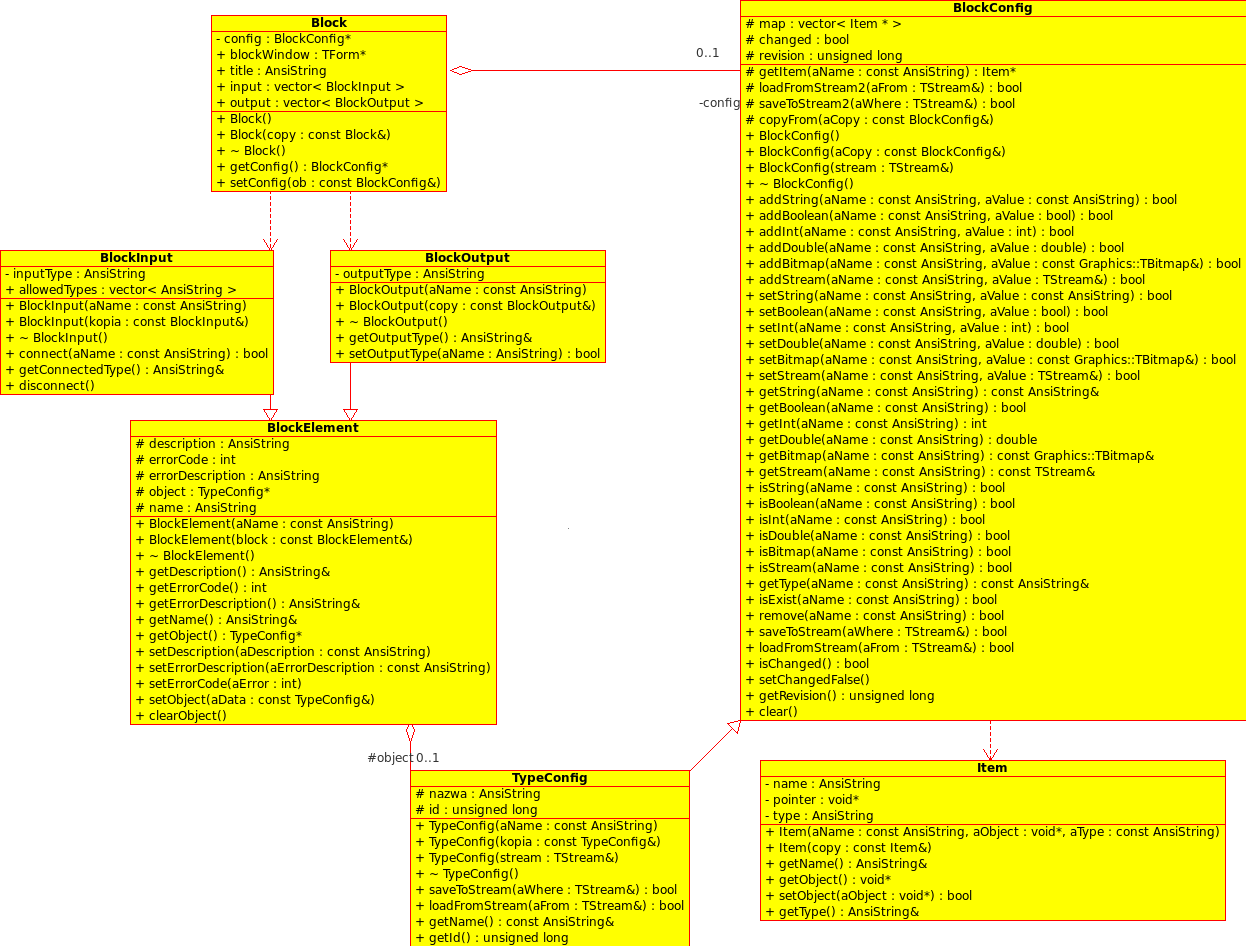
\includegraphics[scale=0.4]{diagram-engine.png}
 \caption{Engine - diagram}
 \label{fig:engine}
\end{figure}
\newpage
\subsection{BRIGE}
Brige - jest odpowiedzialny za pluginy (wtyczki). Obsługuję on pliki dll w których znajdują się typy danych danych lub funkjcę realizujące poszczególne algorytmy przetwarzania obrazów.
Główną opcją jest przeszukiwanie folderów w celu odnalezienie plików dll oraz ini w których jest zawarty opis dll-a. Ta część projektu w głównej mierze narzuca sposób pisania wtyczek, czyli jakie funkcję muszą się znajdować wewnątrz dll oraz definicję tych funkcji czyli jakie argumnety przyjmuje oraz zwraca. Wszystkie algorytmy w programie są uruchamiane poprzez tą klasę,
to w niej są zawarte wskaźniki do funkcji zawartych w plikach dll.
\begin{figure}[h]
 \centering
 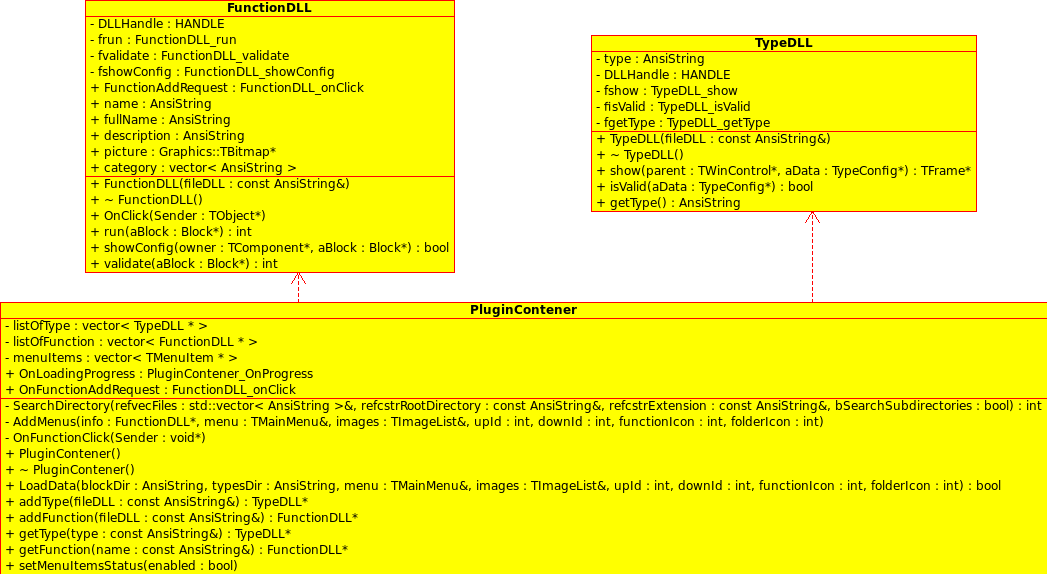
\includegraphics[scale=0.4]{diagram-brige.png}
 \caption{Engine - BRIGE}
 \label{fig:brige}
\end{figure}
\newpage
\subsection{GUI}
GUI - czyli interfejs graficzny, czyli to co zwykłego śmiertelnika najbardziej interesuję. Znajdują się tu klassy odpowiedzialne miedzy innymi za rysowanie bloczków, połączeń - lini, toolbara, historii.
Wszystkie operację które użytkownik wykonuję pracując na programie (oprócz tworzenia wtyczek) są realizowane poprzez te obiekty, które komunikują się z brige lub engine. 
\begin{figure}[h]
 \centering
 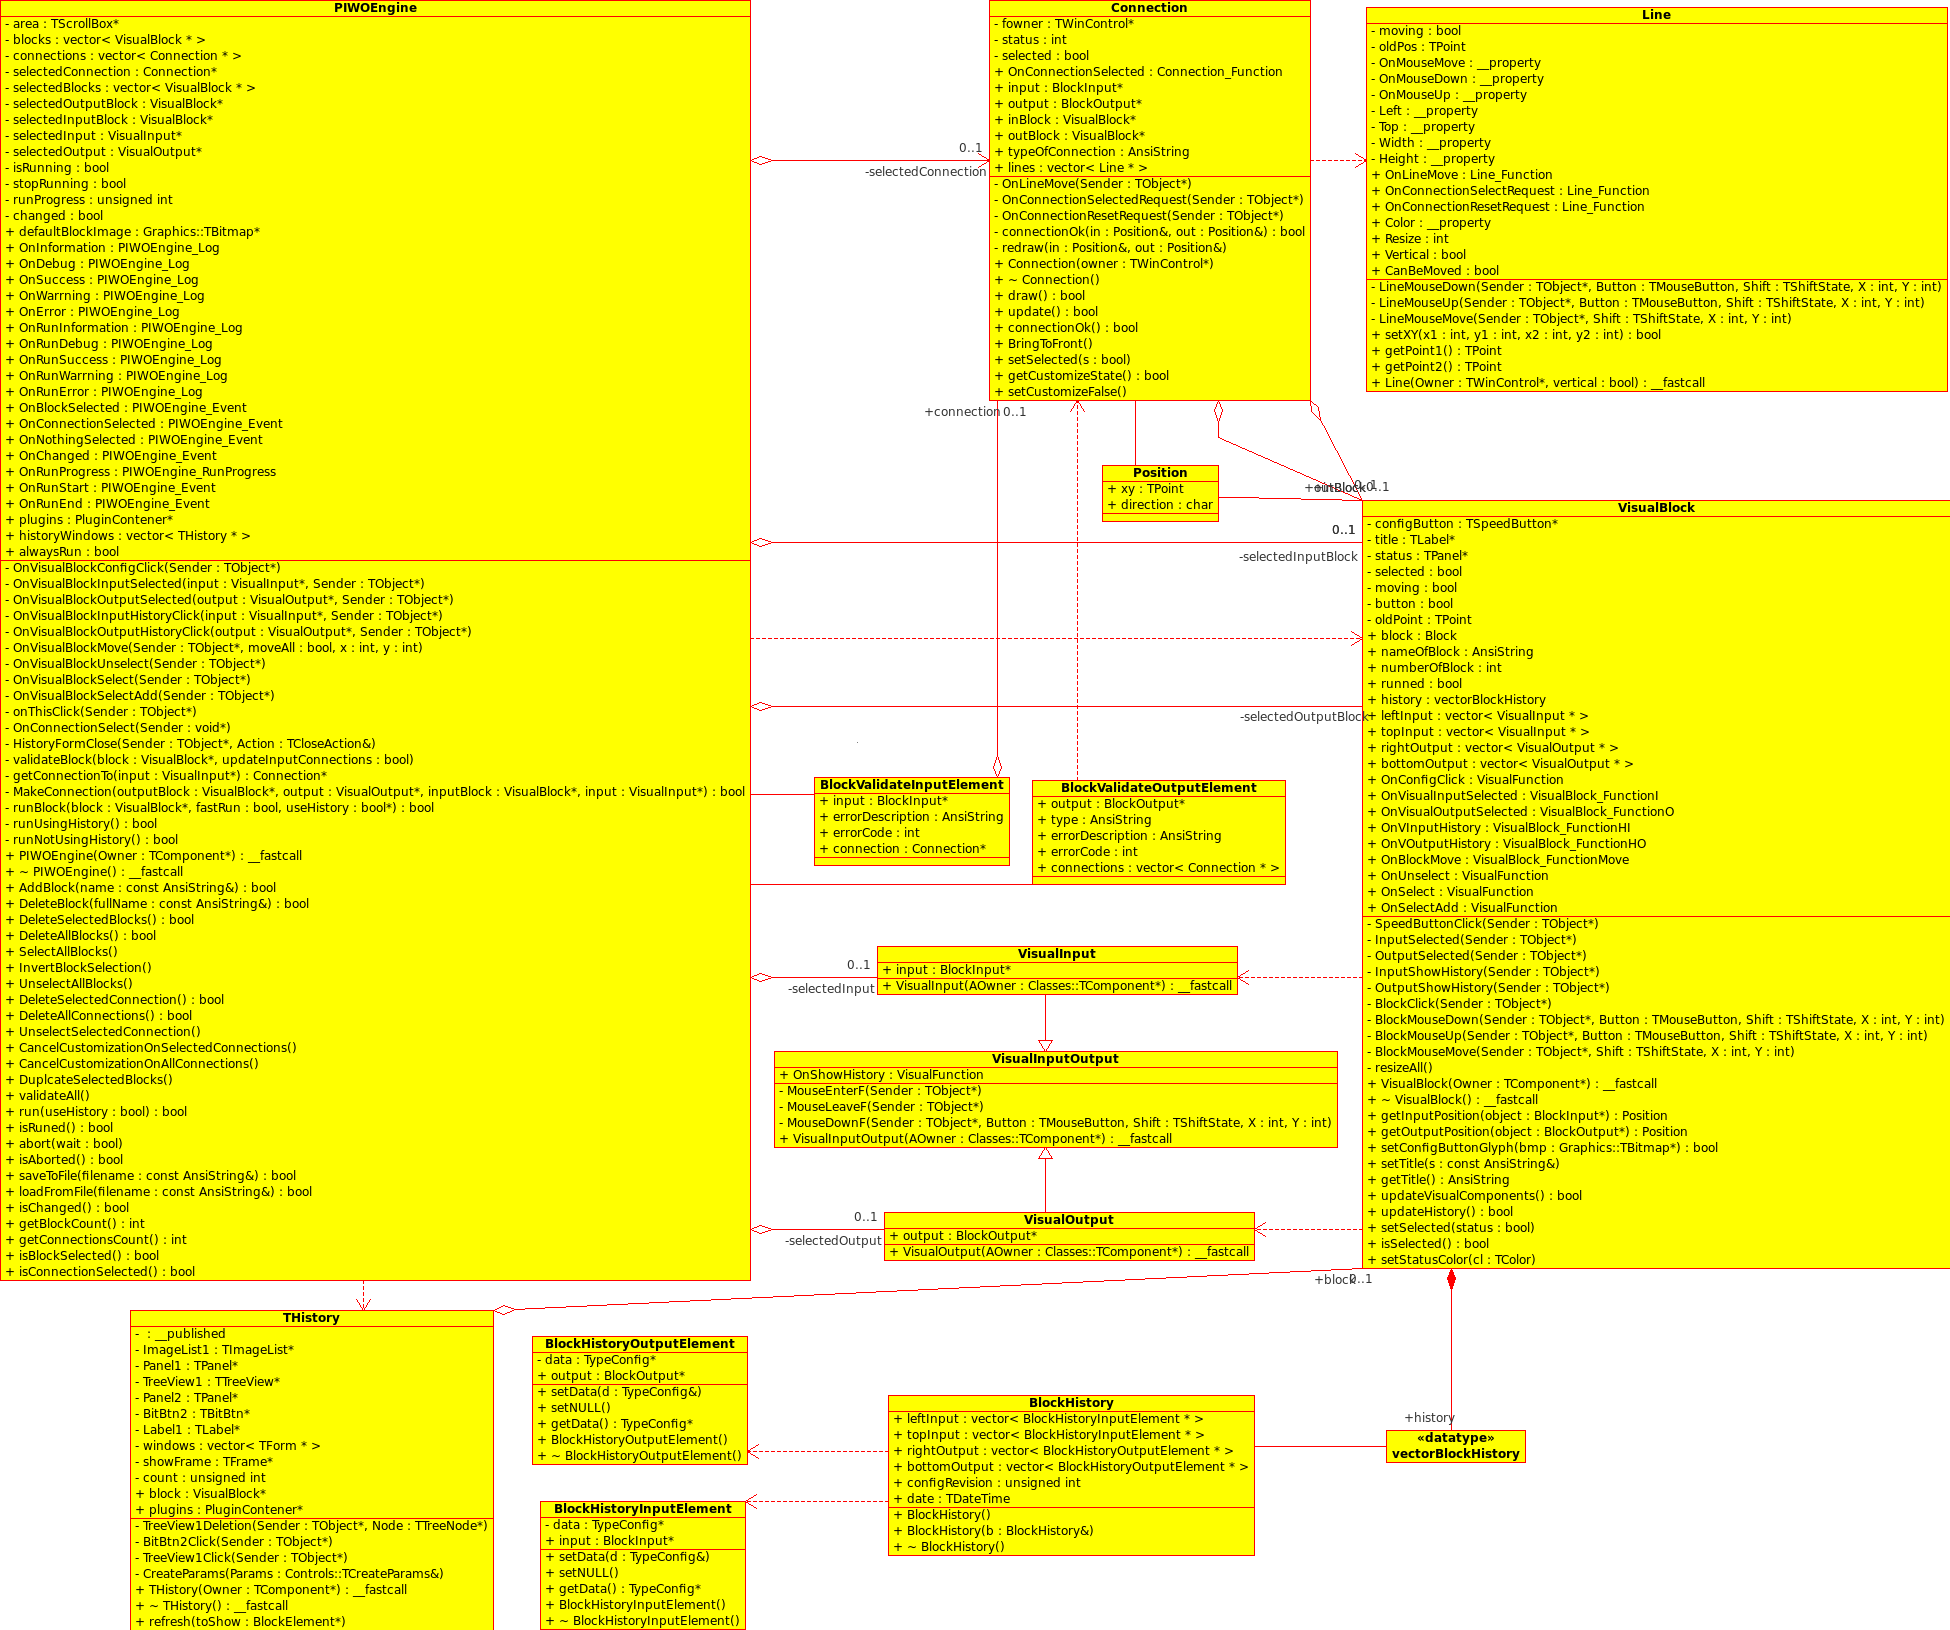
\includegraphics[scale=0.3]{diagram-gui.png}
 \caption{Engine - GUI}
 \label{fig:gui}
\end{figure}
\newpage
\section{Pluginy}
Program obsługuje 2 typy pluginów:
\begin{itemize}
\item pluginy typów
\item pluginy bloków
\end{itemize}
Pluginy typów dostarczją aplikacji obsługi nowych typów danych, aczkolwiek aplikacja i tak poprawnie uruchomi bloczki korzystające z niewspieranych typów, haczyk jest w tym że niekture opcje takie jak podgląd nie będą dostępne dla danego typu.
Informacje o typie danych są zapisywane w klasie TypeConfig.\\

Każda DLL pluginu jest ładowana do pamięci tylko RAZ.
Wymagania nałożone na każdą DLL pełniącą rolę pluginu:
\begin{itemize}
\item Każda DLL musi zawierać: \#pragma link ``MEMMGR.LIB''
\item Każda DLL musi być dostarczona w formie Release.
\item Każda DLL musi być skompilowana z opcją: Packages->Build with runtime packages(true) = vcl;rtl;vclx
\item Każda DLL musi być skompilowana z opcją: Linker->Linking->Use dynamic RTL = false
\end{itemize}
\subsection{Struktura DLL typu i wymagania}
Każda DLL typu musi powprawnie implementować i exportować następujące funkcje:\\
\textit{TFrame\* \_\_stdcall show(TWinControl\* owner, TypeConfig\* aData);}\\
Zadaniem tej funkcji jest poprawne wuświetlenie typu danych. Programista musi zaprojektować własną klase pochodną od TFrame na której w sposób wizualnie poprawny, nizależny od szerokości Frame ma wyświetlić dane zawarte w aData.Po poprawnym stworzeniu takiego obiektu narzucając mu owner który jest przesyłany w paametrze funkcji jak i Parent ma zwrócić wskaźnik do dopiero co utworzonego i wypełnionego danymi Frame.\\\\

\textit{bool \_\_stdcall isValid(TypeConfig\* aData);}\\
Zadaniem tej funkcji jest sprawdzenie poprawności typu. Funkcja musi sprawdzić typ aData, dane w nim zawartym, czy są poprawne i czy są odpowiedniego typu i zwrócić true w przypadku gdy typ jest poprawny, false gdy nie jest.\\\\
\textit{AnsiString \_\_stdcall getType();}\\
Funkcja ta ma tylko i wyłącznie zwrócić nazwę typu danych.

\subsection{Interfejsy typów}
Mianem interfejsu typu okresla się klasę z statycznymi metodami służacymi do tworzenia nowego typu pustego typu danych, zapisywania do niego i odczytywania z niego.
\subsection{Struktura DLL funkcji i wymagania}
W każdej z funkcji programista posiada pełną władze nad obiektem aBlock który symbolizuje blok.
Każda DLL funkcji musi implementować i eksportować następujące funkcje:\\
\textit{bool \_\_stdcall showConfig(TComponent \*owner, Block \*aBlock);}\\
Funkcja ta ma za zadanie pokazać okienko konfiguracyjne bloczka, po jej zakończeniu niemoże ona zostawiać aktywnego okna chyba że okno to jest powiązane z aBlock->blockWindow. Argument owner powinien być parentem i właścicielem nowo stworzonego okna. W interesie programującego jest zapewnić poprawne usunięcie okna z pamięci z wyjątkiem przypadku w którym okno jest powiązane z aBlock->blockWindow. Programista może tu zwrócić false w przypadku gdy niepotrzebuje aby bloczek miał okno konfiguracyjne, w innym przypadku powinien zwrócić true. Funkcja ta jest wywoływana tylko w przypadku gdy użytkownik jawnie kliknie w przycisk konfiguracyjny znajdujący się w centrum bloczka. Zabrania się odwołania do danych w tej funkcji, jak i modyfikacji wejść wyjść. Wszystkie dane które programista chce przechować powinny być przechowywane w klasie aBlock->getConfig().\\\\
\textit{int \_\_stdcall validate(Block \*aBlock);}
Funkcja ta jest wywoływana gdy:\\
\begin{itemize}
\item bloczek zostanie dodany do projektu
\item bloczek zostanie zduplikowany
\item zostanie dodane połączenie do bloczka (dotyczy tylko wejść)
\item zostanie usunięte połączenie do bloczka (dotyczy tylko wejść)
\item typ danych na dowolnym wejściu zostanie zmodyfikowany
\end{itemize}
\\
Funkcja powinna zwracać:\\
0 - gdy nie wprowadzono żadnych zmian w obiekcie aBlock\\
1 - gdy zmodyfikowano tylko kody błedów, opisy, typy danych\\
2 - gdy dodano nowe wejście / wyjście\\\\
W aktualnej wersji engine zwracany kod przez ta funkcje niema dużego wpływu na przetwarzanie projektu/bloku. Aczkolwiek w późniejszej wersji może to ulec zmianie, a poprawne zwracanie kodów może znacznie przyspieszyć działanie programu. Celem programisty w tej funkcji jest poprawne zarządzanie wejściami i wyjściami z bloku, inicjowanie konfiguracji. Programista ma nieograniczoną władzę nad wejsciami i wyjściami z bloku, może zarządzać typami danych jakie moga być podłączone do konkretnego wejścia, decydowac o typie danych jakie będzie dostarczone na wyjście i to właśnie tutaj musi o tym decydować. Kody błędów jakie wolno ustawić na wejściu / wyjściu to: 0 - wszystko ok, 1 - warrning. Kod 2- error jest zastrzeżony tylko i wyłącznie dla funkcji run.\\\\
\textit{int \_\_stdcall run(Block \*aBlock);}\\
Zadaniem funkcji jest wykonanie operacji ściśle powiązanej z bloczkiem. Jest to jedyna funkcja w której programista ma 100\% dostep do danych.\\\\
Kody wyjścia:\\
0 - wszystko ok\\
1 - warrning, coś nie zostało wykonane ale program może kontynuować\\
2 - error\\
\\
Programista w tej funkcji niemoże:\\
- dodawać, usuwać wejśc\\
- dodawać, usuwać wyjśc\\
- modyfikować typu danych na wyjściach\\
- modyfikować listy dozwolonych typów na wejściach\\
- odłączać połączenia podłączonego do wejścia\\
\\
Programista w tej funkcji ma obowiązek:\\
- poprawnie zwracać kody wyjść\\
- zwalniać pamięć po obiektach\\

\chapter{Class Index}
\section{Hierarchia klas}
Ta lista dziedziczenia posortowana jest z grubsza, choć nie całkowicie, alfabetycznie:\begin{CompactList}
\item \contentsline{section}{Block}{\pageref{class_block}}{}
\item \contentsline{section}{BlockConfig}{\pageref{class_block_config}}{}
\begin{CompactList}
\item \contentsline{section}{TypeConfig}{\pageref{class_type_config}}{}
\end{CompactList}
\item \contentsline{section}{BlockElement}{\pageref{class_block_element}}{}
\begin{CompactList}
\item \contentsline{section}{BlockInput}{\pageref{class_block_input}}{}
\item \contentsline{section}{BlockOutput}{\pageref{class_block_output}}{}
\end{CompactList}
\item \contentsline{section}{FunctionDLL}{\pageref{class_function_d_l_l}}{}
\item \contentsline{section}{Item}{\pageref{class_item}}{}
\item \contentsline{section}{PluginContener}{\pageref{class_plugin_contener}}{}
\end{CompactList}

\chapter{Class Index}
\section{Class List}
Here are the classes, structs, unions and interfaces with brief descriptions:\begin{CompactList}
\item\contentsline{section}{\hyperlink{class_block_config}{BlockConfig} }{\pageref{class_block_config}}{}
\item\contentsline{section}{\hyperlink{class_item}{Item} }{\pageref{class_item}}{}
\end{CompactList}

\chapter{File Index}
\section{File List}
Here is a list of all files with brief descriptions:\begin{CompactList}
\item\contentsline{section}{/PIWO/Program/\hyperlink{main_8cpp}{main.cpp} }{\pageref{main_8cpp}}{}
\item\contentsline{section}{/PIWO/Program/\hyperlink{main_8h}{main.h} }{\pageref{main_8h}}{}
\item\contentsline{section}{/PIWO/Program/\hyperlink{PIWO_8cpp}{PIWO.cpp} }{\pageref{PIWO_8cpp}}{}
\item\contentsline{section}{/PIWO/Program/\hyperlink{splash_8cpp}{splash.cpp} }{\pageref{splash_8cpp}}{}
\item\contentsline{section}{/PIWO/Program/\hyperlink{splash_8h}{splash.h} }{\pageref{splash_8h}}{}
\item\contentsline{section}{/PIWO/Program/\hyperlink{Unit4_8cpp}{Unit4.cpp} }{\pageref{Unit4_8cpp}}{}
\item\contentsline{section}{/PIWO/Program/\hyperlink{Unit4_8h}{Unit4.h} }{\pageref{Unit4_8h}}{}
\item\contentsline{section}{/PIWO/Program/\hyperlink{Unit5_8cpp}{Unit5.cpp} }{\pageref{Unit5_8cpp}}{}
\item\contentsline{section}{/PIWO/Program/\hyperlink{Unit5_8h}{Unit5.h} }{\pageref{Unit5_8h}}{}
\item\contentsline{section}{/PIWO/Program/brige/\hyperlink{FunctionDLL_8cpp}{FunctionDLL.cpp} }{\pageref{FunctionDLL_8cpp}}{}
\item\contentsline{section}{/PIWO/Program/brige/\hyperlink{FunctionDLL_8h}{FunctionDLL.h} }{\pageref{FunctionDLL_8h}}{}
\item\contentsline{section}{/PIWO/Program/brige/\hyperlink{PluginContener_8cpp}{PluginContener.cpp} }{\pageref{PluginContener_8cpp}}{}
\item\contentsline{section}{/PIWO/Program/brige/\hyperlink{PluginContener_8h}{PluginContener.h} }{\pageref{PluginContener_8h}}{}
\item\contentsline{section}{/PIWO/Program/brige/\hyperlink{TypeDLL_8cpp}{TypeDLL.cpp} }{\pageref{TypeDLL_8cpp}}{}
\item\contentsline{section}{/PIWO/Program/brige/\hyperlink{TypeDLL_8h}{TypeDLL.h} }{\pageref{TypeDLL_8h}}{}
\item\contentsline{section}{/PIWO/Program/engine/\hyperlink{Block_8cpp}{Block.cpp} }{\pageref{Block_8cpp}}{}
\item\contentsline{section}{/PIWO/Program/engine/\hyperlink{Block_8h}{Block.h} }{\pageref{Block_8h}}{}
\item\contentsline{section}{/PIWO/Program/engine/\hyperlink{BlockConfig_8cpp}{BlockConfig.cpp} }{\pageref{BlockConfig_8cpp}}{}
\item\contentsline{section}{/PIWO/Program/engine/\hyperlink{BlockConfig_8h}{BlockConfig.h} }{\pageref{BlockConfig_8h}}{}
\item\contentsline{section}{/PIWO/Program/engine/\hyperlink{BlockElement_8cpp}{BlockElement.cpp} }{\pageref{BlockElement_8cpp}}{}
\item\contentsline{section}{/PIWO/Program/engine/\hyperlink{BlockElement_8h}{BlockElement.h} }{\pageref{BlockElement_8h}}{}
\item\contentsline{section}{/PIWO/Program/engine/\hyperlink{BlockInput_8cpp}{BlockInput.cpp} }{\pageref{BlockInput_8cpp}}{}
\item\contentsline{section}{/PIWO/Program/engine/\hyperlink{BlockInput_8h}{BlockInput.h} }{\pageref{BlockInput_8h}}{}
\item\contentsline{section}{/PIWO/Program/engine/\hyperlink{BlockOutput_8cpp}{BlockOutput.cpp} }{\pageref{BlockOutput_8cpp}}{}
\item\contentsline{section}{/PIWO/Program/engine/\hyperlink{BlockOutput_8h}{BlockOutput.h} }{\pageref{BlockOutput_8h}}{}
\item\contentsline{section}{/PIWO/Program/engine/\hyperlink{Item_8cpp}{Item.cpp} }{\pageref{Item_8cpp}}{}
\item\contentsline{section}{/PIWO/Program/engine/\hyperlink{Item_8h}{Item.h} }{\pageref{Item_8h}}{}
\item\contentsline{section}{/PIWO/Program/engine/\hyperlink{TypeConfig_8cpp}{TypeConfig.cpp} }{\pageref{TypeConfig_8cpp}}{}
\item\contentsline{section}{/PIWO/Program/engine/\hyperlink{TypeConfig_8h}{TypeConfig.h} }{\pageref{TypeConfig_8h}}{}
\item\contentsline{section}{/PIWO/Program/gui/\hyperlink{BlockHistory_8cpp}{BlockHistory.cpp} }{\pageref{BlockHistory_8cpp}}{}
\item\contentsline{section}{/PIWO/Program/gui/\hyperlink{BlockHistory_8h}{BlockHistory.h} }{\pageref{BlockHistory_8h}}{}
\item\contentsline{section}{/PIWO/Program/gui/\hyperlink{BlockHistoryInputElement_8cpp}{BlockHistoryInputElement.cpp} }{\pageref{BlockHistoryInputElement_8cpp}}{}
\item\contentsline{section}{/PIWO/Program/gui/\hyperlink{BlockHistoryInputElement_8h}{BlockHistoryInputElement.h} }{\pageref{BlockHistoryInputElement_8h}}{}
\item\contentsline{section}{/PIWO/Program/gui/\hyperlink{BlockHistoryOutputElement_8cpp}{BlockHistoryOutputElement.cpp} }{\pageref{BlockHistoryOutputElement_8cpp}}{}
\item\contentsline{section}{/PIWO/Program/gui/\hyperlink{BlockHistoryOutputElement_8h}{BlockHistoryOutputElement.h} }{\pageref{BlockHistoryOutputElement_8h}}{}
\item\contentsline{section}{/PIWO/Program/gui/\hyperlink{BlockValidateInputElement_8h}{BlockValidateInputElement.h} }{\pageref{BlockValidateInputElement_8h}}{}
\item\contentsline{section}{/PIWO/Program/gui/\hyperlink{BlockValidateOutputElement_8h}{BlockValidateOutputElement.h} }{\pageref{BlockValidateOutputElement_8h}}{}
\item\contentsline{section}{/PIWO/Program/gui/\hyperlink{Connection_8cpp}{Connection.cpp} }{\pageref{Connection_8cpp}}{}
\item\contentsline{section}{/PIWO/Program/gui/\hyperlink{Connection_8h}{Connection.h} }{\pageref{Connection_8h}}{}
\item\contentsline{section}{/PIWO/Program/gui/\hyperlink{history_8cpp}{history.cpp} }{\pageref{history_8cpp}}{}
\item\contentsline{section}{/PIWO/Program/gui/\hyperlink{history_8h}{history.h} }{\pageref{history_8h}}{}
\item\contentsline{section}{/PIWO/Program/gui/\hyperlink{Line_8cpp}{Line.cpp} }{\pageref{Line_8cpp}}{}
\item\contentsline{section}{/PIWO/Program/gui/\hyperlink{Line_8h}{Line.h} }{\pageref{Line_8h}}{}
\item\contentsline{section}{/PIWO/Program/gui/\hyperlink{PIWOEngine_8cpp}{PIWOEngine.cpp} }{\pageref{PIWOEngine_8cpp}}{}
\item\contentsline{section}{/PIWO/Program/gui/\hyperlink{PIWOEngine_8h}{PIWOEngine.h} }{\pageref{PIWOEngine_8h}}{}
\item\contentsline{section}{/PIWO/Program/gui/\hyperlink{VisualBlock_8cpp}{VisualBlock.cpp} }{\pageref{VisualBlock_8cpp}}{}
\item\contentsline{section}{/PIWO/Program/gui/\hyperlink{VisualBlock_8h}{VisualBlock.h} }{\pageref{VisualBlock_8h}}{}
\item\contentsline{section}{/PIWO/Program/gui/\hyperlink{VisualInput_8cpp}{VisualInput.cpp} }{\pageref{VisualInput_8cpp}}{}
\item\contentsline{section}{/PIWO/Program/gui/\hyperlink{VisualInput_8h}{VisualInput.h} }{\pageref{VisualInput_8h}}{}
\item\contentsline{section}{/PIWO/Program/gui/\hyperlink{VisualInputOutput_8cpp}{VisualInputOutput.cpp} }{\pageref{VisualInputOutput_8cpp}}{}
\item\contentsline{section}{/PIWO/Program/gui/\hyperlink{VisualInputOutput_8h}{VisualInputOutput.h} }{\pageref{VisualInputOutput_8h}}{}
\item\contentsline{section}{/PIWO/Program/gui/\hyperlink{VisualOutput_8cpp}{VisualOutput.cpp} }{\pageref{VisualOutput_8cpp}}{}
\item\contentsline{section}{/PIWO/Program/gui/\hyperlink{VisualOutput_8h}{VisualOutput.h} }{\pageref{VisualOutput_8h}}{}
\end{CompactList}

\chapter{Class Documentation}
\hypertarget{classBlock}{
\section{Block Class Reference}
\label{classBlock}\index{Block@{Block}}
}
{\tt \#include $<$Block.h$>$}

Collaboration diagram for Block:\nopagebreak
\begin{figure}[H]
\begin{center}
\leavevmode
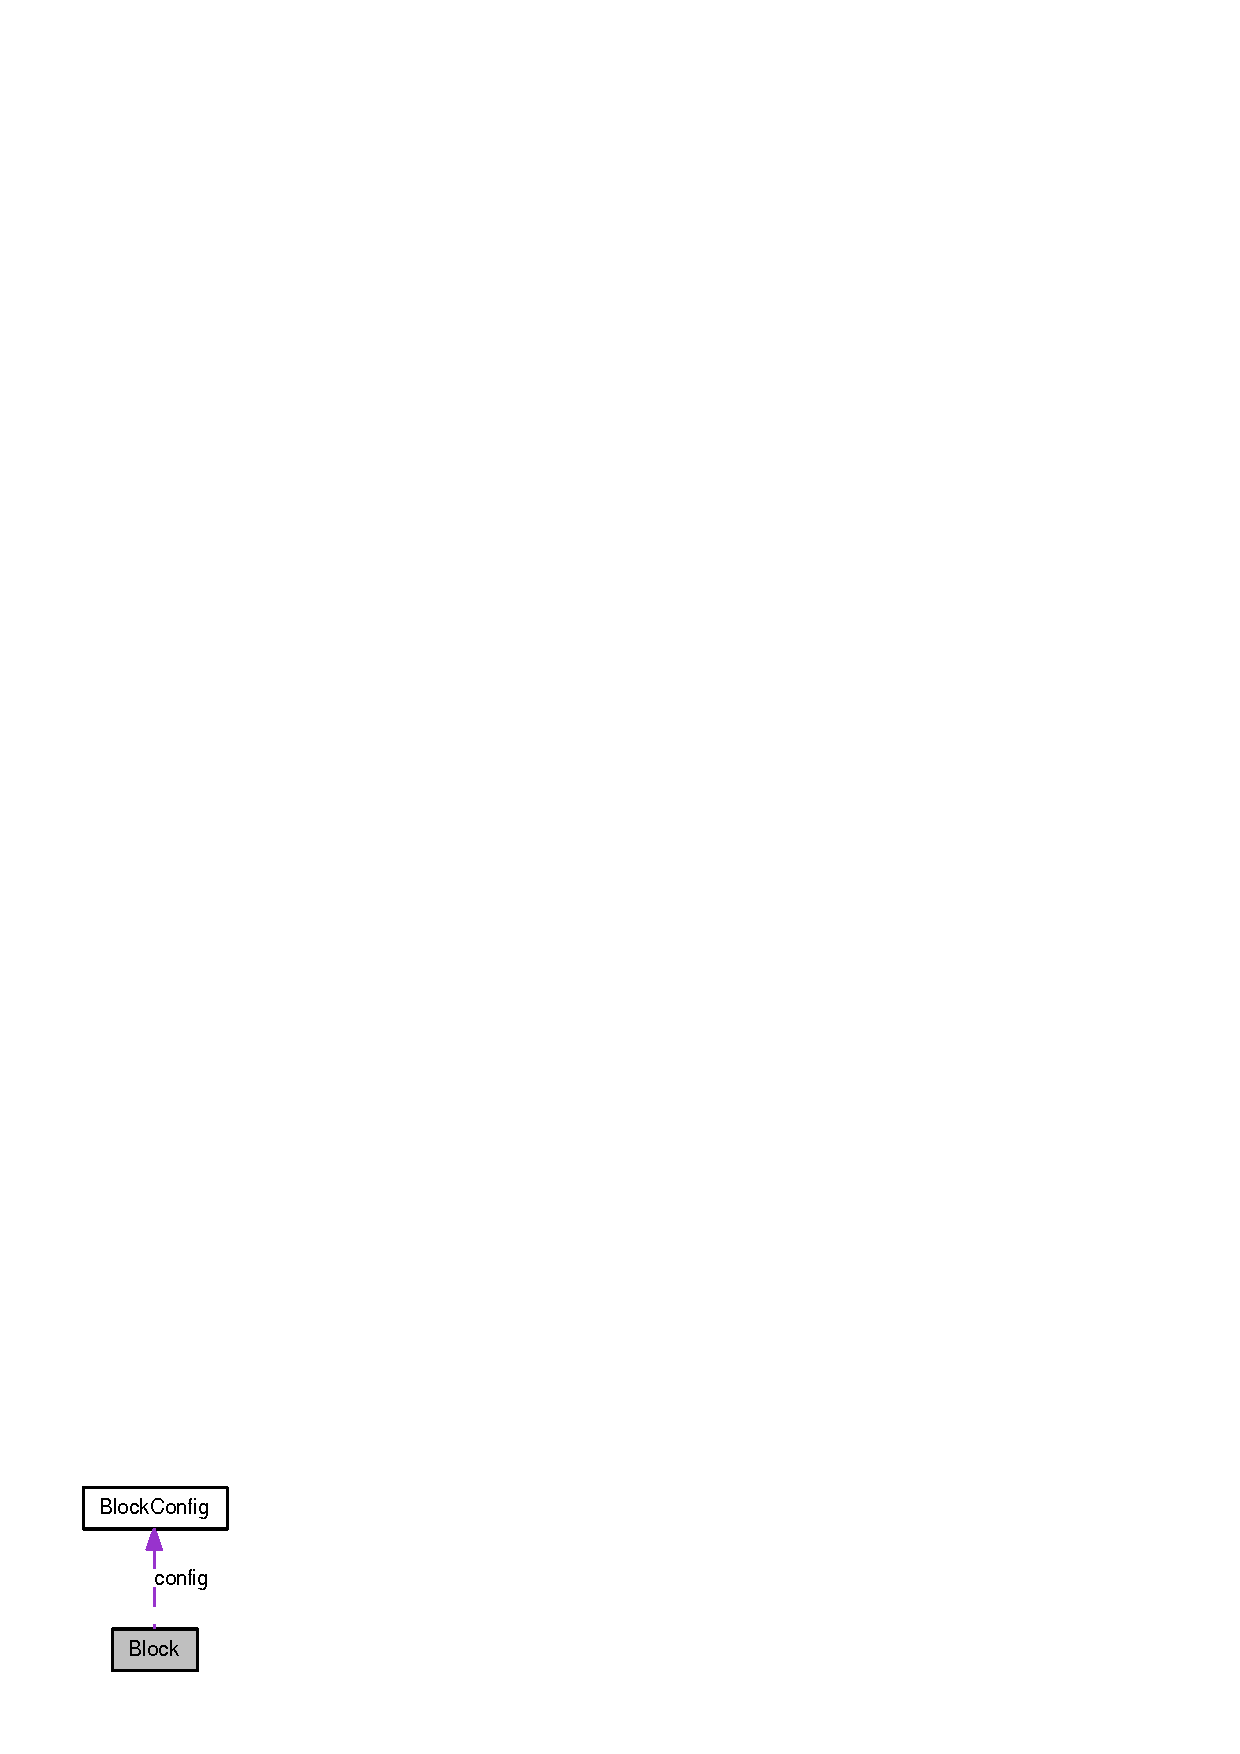
\includegraphics[width=56pt]{classBlock__coll__graph}
\end{center}
\end{figure}
\subsection*{Public Member Functions}
\begin{CompactItemize}
\item 
\hyperlink{classBlock_37658a946bf5067ad01d68d9ff086adc}{Block} ()
\item 
\hyperlink{classBlock_eaf94aa618003b452d8b6f32d1e23766}{Block} (const \hyperlink{classBlock}{Block} \&copy)
\item 
\hyperlink{classBlock_19d1bd0e1cef6a865ed2745a2e648405}{$\sim$Block} ()
\item 
\hyperlink{classBlockConfig}{BlockConfig} $\ast$ \hyperlink{classBlock_17985f527bea557c7da9279424d96ccc}{getConfig} ()
\item 
void \hyperlink{classBlock_703019dc511468104b327bff7dd779d2}{setConfig} (const \hyperlink{classBlockConfig}{BlockConfig} \&ob)
\end{CompactItemize}
\subsection*{Public Attributes}
\begin{CompactItemize}
\item 
TForm $\ast$ \hyperlink{classBlock_64bbe660cd95004706c7f5158d8e270b}{blockWindow}
\item 
AnsiString \hyperlink{classBlock_9c89fafbe64236bc46ade38d458712b1}{title}
\item 
vector$<$ \hyperlink{classBlockInput}{BlockInput} $>$ \hyperlink{classBlock_6a6c2c1e8c3fd4219d8cc7e9f099205b}{input}
\item 
vector$<$ \hyperlink{classBlockOutput}{BlockOutput} $>$ \hyperlink{classBlock_7afddb4a8f6063e0b05dbdd1f17cf07f}{output}
\end{CompactItemize}
\subsection*{Private Attributes}
\begin{CompactItemize}
\item 
\hyperlink{classBlockConfig}{BlockConfig} $\ast$ \hyperlink{classBlock_0f49dcd75a7694f73558ac602b2b3d1f}{config}
\end{CompactItemize}


\subsection{Detailed Description}
\hyperlink{classBlock}{Block} - Klasa pojemnik przechowujaca wejscia i wyjscia bloku \begin{Desc}
\item[Author:]Piotr \end{Desc}
\begin{Desc}
\item[Date:]2008.11.25 \end{Desc}
\begin{Desc}
\item[Version:]0.1 \end{Desc}


Definition at line 21 of file Block.h.

\subsection{Constructor \& Destructor Documentation}
\hypertarget{classBlock_37658a946bf5067ad01d68d9ff086adc}{
\index{Block@{Block}!Block@{Block}}
\index{Block@{Block}!Block@{Block}}
\subsubsection[Block]{\setlength{\rightskip}{0pt plus 5cm}Block::Block ()}}
\label{classBlock_37658a946bf5067ad01d68d9ff086adc}


Konstruktor domyslny. 

Definition at line 3 of file Block.cpp.

References blockWindow, config, and title.\hypertarget{classBlock_eaf94aa618003b452d8b6f32d1e23766}{
\index{Block@{Block}!Block@{Block}}
\index{Block@{Block}!Block@{Block}}
\subsubsection[Block]{\setlength{\rightskip}{0pt plus 5cm}Block::Block (const {\bf Block} \& {\em copy})}}
\label{classBlock_eaf94aa618003b452d8b6f32d1e23766}


Konstruktor kopiujacy \begin{Desc}
\item[Parameters:]
\begin{description}
\item[{\em copy}]obiekt ktory zostanie skopiowany \end{description}
\end{Desc}


Definition at line 10 of file Block.cpp.

References blockWindow, config, input, output, and title.\hypertarget{classBlock_19d1bd0e1cef6a865ed2745a2e648405}{
\index{Block@{Block}!$\sim$Block@{$\sim$Block}}
\index{$\sim$Block@{$\sim$Block}!Block@{Block}}
\subsubsection[$\sim$Block]{\setlength{\rightskip}{0pt plus 5cm}Block::$\sim$Block ()}}
\label{classBlock_19d1bd0e1cef6a865ed2745a2e648405}


Destruktor 

Definition at line 19 of file Block.cpp.

References blockWindow, and config.

\subsection{Member Function Documentation}
\hypertarget{classBlock_17985f527bea557c7da9279424d96ccc}{
\index{Block@{Block}!getConfig@{getConfig}}
\index{getConfig@{getConfig}!Block@{Block}}
\subsubsection[getConfig]{\setlength{\rightskip}{0pt plus 5cm}{\bf BlockConfig} $\ast$ Block::getConfig ()}}
\label{classBlock_17985f527bea557c7da9279424d96ccc}


Zwraca wskaznik do uwstawien bloku. \begin{Desc}
\item[Returns:]ustawienia bloku. \end{Desc}


Definition at line 30 of file Block.cpp.

References config.

Referenced by PIWOEngine::loadFromFile(), PIWOEngine::OnVisualBlockConfigClick(), PIWOEngine::runBlock(), and VisualBlock::updateHistory().\hypertarget{classBlock_703019dc511468104b327bff7dd779d2}{
\index{Block@{Block}!setConfig@{setConfig}}
\index{setConfig@{setConfig}!Block@{Block}}
\subsubsection[setConfig]{\setlength{\rightskip}{0pt plus 5cm}void Block::setConfig (const {\bf BlockConfig} \& {\em ob})}}
\label{classBlock_703019dc511468104b327bff7dd779d2}


Ustawia wlasciwosci obiektu. \begin{Desc}
\item[Parameters:]
\begin{description}
\item[{\em ob}]wlasciowsci obiektu. \end{description}
\end{Desc}


Definition at line 35 of file Block.cpp.

References config.

Referenced by PIWOEngine::DuplcateSelectedBlocks().

\subsection{Member Data Documentation}
\hypertarget{classBlock_0f49dcd75a7694f73558ac602b2b3d1f}{
\index{Block@{Block}!config@{config}}
\index{config@{config}!Block@{Block}}
\subsubsection[config]{\setlength{\rightskip}{0pt plus 5cm}{\bf BlockConfig}$\ast$ {\bf Block::config}\hspace{0.3cm}{\tt  \mbox{[}private\mbox{]}}}}
\label{classBlock_0f49dcd75a7694f73558ac602b2b3d1f}




Definition at line 24 of file Block.h.

Referenced by Block(), getConfig(), setConfig(), and $\sim$Block().\hypertarget{classBlock_64bbe660cd95004706c7f5158d8e270b}{
\index{Block@{Block}!blockWindow@{blockWindow}}
\index{blockWindow@{blockWindow}!Block@{Block}}
\subsubsection[blockWindow]{\setlength{\rightskip}{0pt plus 5cm}TForm$\ast$ {\bf Block::blockWindow}}}
\label{classBlock_64bbe660cd95004706c7f5158d8e270b}


Wskaznik do okna, mozliwy do uzycia w przypadku tworzenia bloczkow potrzebujacych zostawic okno po wykonaniu akcji run. 

Definition at line 29 of file Block.h.

Referenced by Block(), and $\sim$Block().\hypertarget{classBlock_9c89fafbe64236bc46ade38d458712b1}{
\index{Block@{Block}!title@{title}}
\index{title@{title}!Block@{Block}}
\subsubsection[title]{\setlength{\rightskip}{0pt plus 5cm}AnsiString {\bf Block::title}}}
\label{classBlock_9c89fafbe64236bc46ade38d458712b1}


Tytul bloczka 

Definition at line 33 of file Block.h.

Referenced by Block(), and VisualBlock::setTitle().\hypertarget{classBlock_6a6c2c1e8c3fd4219d8cc7e9f099205b}{
\index{Block@{Block}!input@{input}}
\index{input@{input}!Block@{Block}}
\subsubsection[input]{\setlength{\rightskip}{0pt plus 5cm}vector$<${\bf BlockInput}$>$ {\bf Block::input}}}
\label{classBlock_6a6c2c1e8c3fd4219d8cc7e9f099205b}


Lista wejsc bloku. 

Definition at line 37 of file Block.h.

Referenced by Block(), PIWOEngine::DuplcateSelectedBlocks(), PIWOEngine::loadFromFile(), PIWOEngine::runBlock(), VisualBlock::updateVisualComponents(), and PIWOEngine::validateBlock().\hypertarget{classBlock_7afddb4a8f6063e0b05dbdd1f17cf07f}{
\index{Block@{Block}!output@{output}}
\index{output@{output}!Block@{Block}}
\subsubsection[output]{\setlength{\rightskip}{0pt plus 5cm}vector$<${\bf BlockOutput}$>$ {\bf Block::output}}}
\label{classBlock_7afddb4a8f6063e0b05dbdd1f17cf07f}


Lista wyjsc bloku. 

Definition at line 41 of file Block.h.

Referenced by Block(), PIWOEngine::DuplcateSelectedBlocks(), PIWOEngine::loadFromFile(), PIWOEngine::runBlock(), VisualBlock::updateVisualComponents(), and PIWOEngine::validateBlock().

The documentation for this class was generated from the following files:\begin{CompactItemize}
\item 
/PIWO/Program/engine/\hyperlink{Block_8h}{Block.h}\item 
/PIWO/Program/engine/\hyperlink{Block_8cpp}{Block.cpp}\end{CompactItemize}

\hypertarget{classBlockConfig}{
\section{BlockConfig Class Reference}
\label{classBlockConfig}\index{BlockConfig@{BlockConfig}}
}
{\tt \#include $<$BlockConfig.h$>$}

Inheritance diagram for BlockConfig:\nopagebreak
\begin{figure}[H]
\begin{center}
\leavevmode
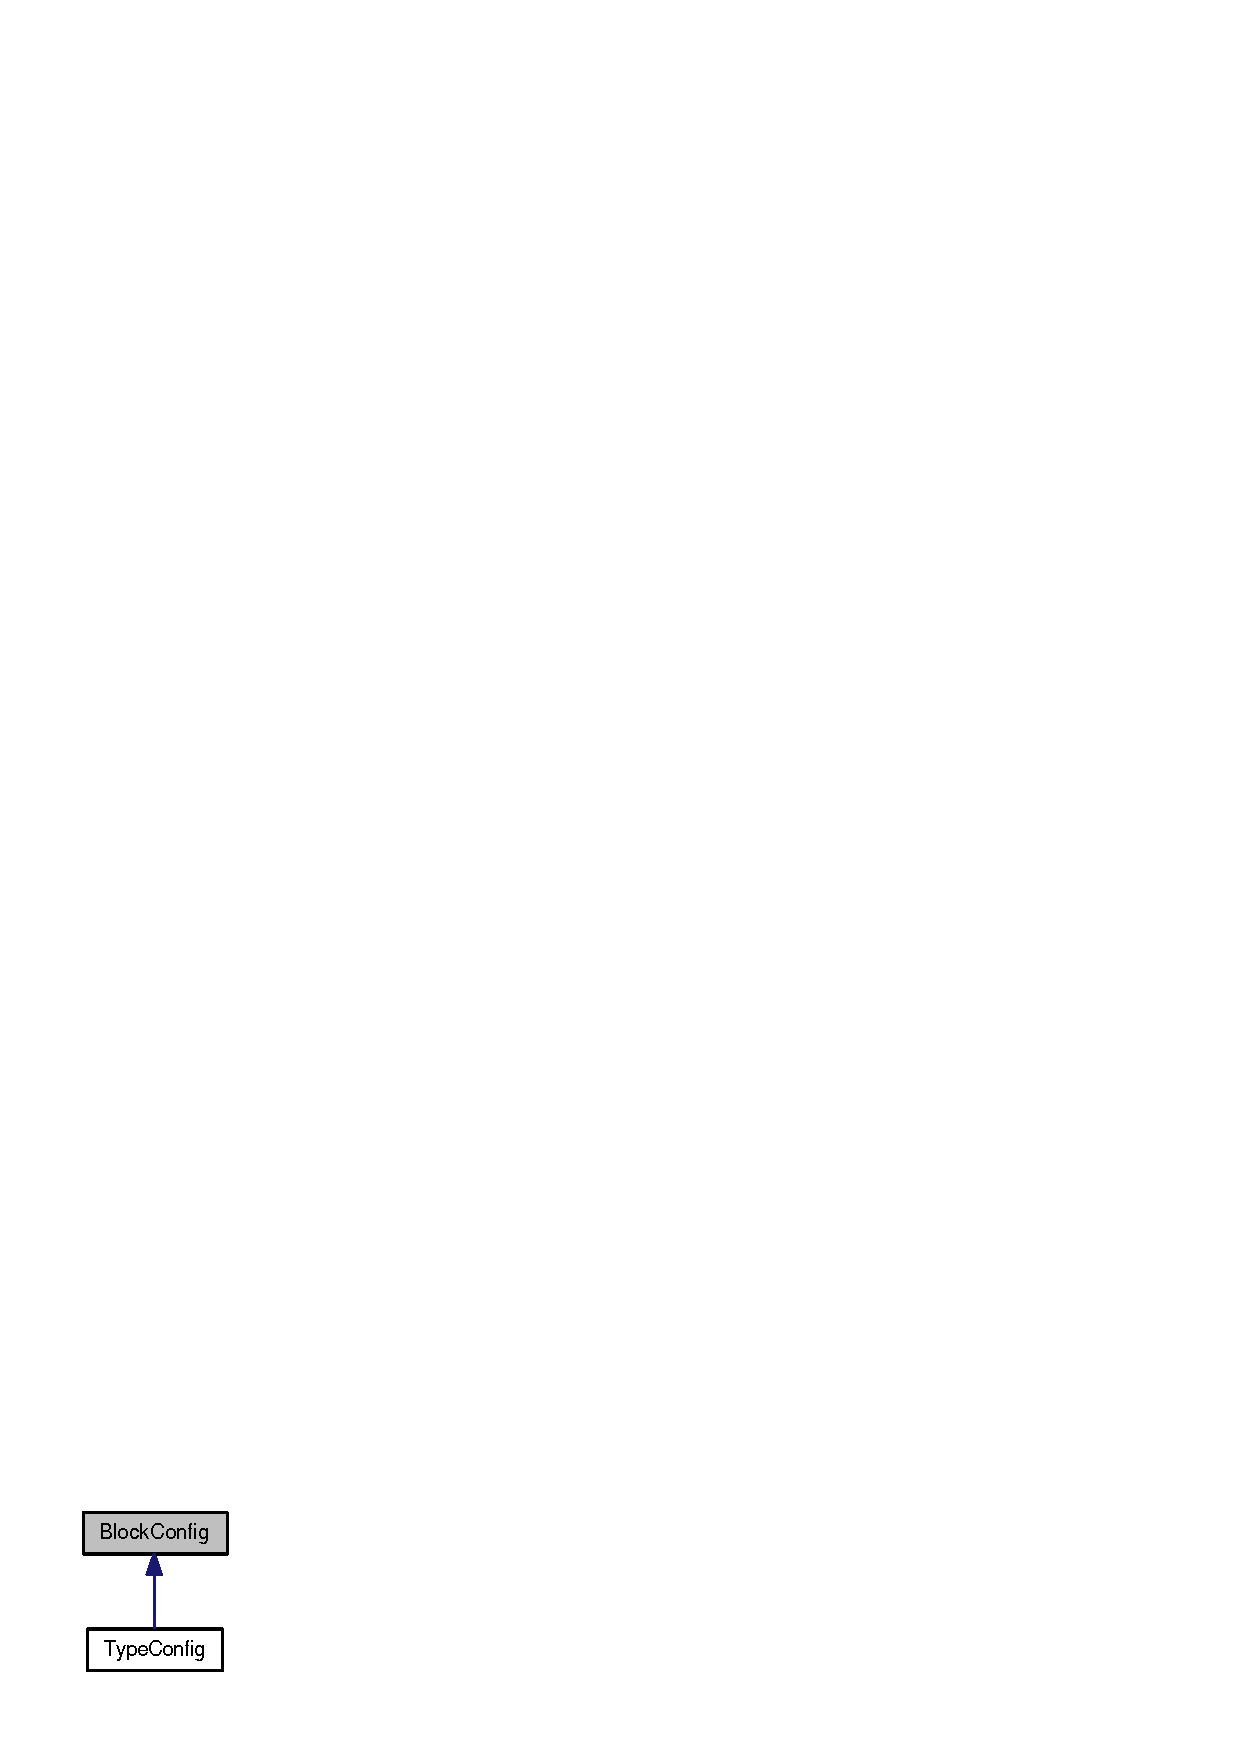
\includegraphics[width=56pt]{classBlockConfig__inherit__graph}
\end{center}
\end{figure}
\subsection*{Public Member Functions}
\begin{CompactItemize}
\item 
\hyperlink{classBlockConfig_e855f45589e5590e9484a7988e87a1bb}{BlockConfig} ()
\item 
\hyperlink{classBlockConfig_a6855fad58eca1c75a8b5e42d02d8efd}{BlockConfig} (const \hyperlink{classBlockConfig}{BlockConfig} \&aCopy)
\item 
\hyperlink{classBlockConfig_c531399ee1d684fe222697bb5a92d81a}{BlockConfig} (TStream \&stream)
\item 
\hyperlink{classBlockConfig_61fe01105c9f6a0c2de8506ed61f1be7}{$\sim$BlockConfig} ()
\item 
bool \hyperlink{classBlockConfig_626645a51f39e02fca6e80a10011c655}{addString} (const AnsiString aName, const AnsiString aValue)
\item 
bool \hyperlink{classBlockConfig_239f38f9b8d09bf6bfa6c0d8c4a27c9d}{addBoolean} (const AnsiString aName, bool aValue)
\item 
bool \hyperlink{classBlockConfig_e0085dac56c5c698621d36dfa7c29095}{addInt} (const AnsiString aName, int aValue)
\item 
bool \hyperlink{classBlockConfig_f53a54f10e34c12c1365a7e695f05f97}{addDouble} (const AnsiString aName, double aValue)
\item 
bool \hyperlink{classBlockConfig_bcb71b475846ba2466568fa010220b80}{addBitmap} (const AnsiString aName, const Graphics::TBitmap \&aValue)
\item 
bool \hyperlink{classBlockConfig_7fb67f78387dbb117ce9ed4bca9edd61}{addStream} (const AnsiString aName, TStream \&aValue)
\item 
bool \hyperlink{classBlockConfig_145d262224797241d4d591675f5dd29c}{setString} (const AnsiString aName, const AnsiString aValue)
\item 
bool \hyperlink{classBlockConfig_4a33af6cdc4c46f5acb0ba5f4a2f29de}{setBoolean} (const AnsiString aName, bool aValue)
\item 
bool \hyperlink{classBlockConfig_e5f32cb1b0194b8570b2eadac34d93fb}{setInt} (const AnsiString aName, int aValue)
\item 
bool \hyperlink{classBlockConfig_093960e3e529de1bbae973d73bb04cf5}{setDouble} (const AnsiString aName, double aValue)
\item 
bool \hyperlink{classBlockConfig_11fee46a607ecdc6fdba8f019229dba5}{setBitmap} (const AnsiString aName, const Graphics::TBitmap \&aValue)
\item 
bool \hyperlink{classBlockConfig_3a2d0d102a3d0a872c407dcea3740bd6}{setStream} (const AnsiString aName, TStream \&aValue)
\item 
const AnsiString \& \hyperlink{classBlockConfig_f5253e606d920aa0861f84e19ccef333}{getString} (const AnsiString aName)
\item 
bool \hyperlink{classBlockConfig_72c6ea45171e485c8d7e38ccceab7b29}{getBoolean} (const AnsiString aName)
\item 
int \hyperlink{classBlockConfig_3786dd56a15961cdf65fe17e37adc61e}{getInt} (const AnsiString aName)
\item 
double \hyperlink{classBlockConfig_a62e41b6cc5c2e4cc509e6e9dded417b}{getDouble} (const AnsiString aName)
\item 
const Graphics::TBitmap \& \hyperlink{classBlockConfig_909bbcbc744629ba3daa077045ab2851}{getBitmap} (const AnsiString aName)
\item 
const TStream \& \hyperlink{classBlockConfig_67172ee311ec7eff44c98196b86f2829}{getStream} (const AnsiString aName)
\item 
bool \hyperlink{classBlockConfig_c48527d78ed04ffd5edf96f1af99b8b7}{isString} (const AnsiString aName)
\item 
bool \hyperlink{classBlockConfig_86efbfd1e6dc6f23c5d32e42b9540312}{isBoolean} (const AnsiString aName)
\item 
bool \hyperlink{classBlockConfig_49b75dae37b27599f6b84d63f035982f}{isInt} (const AnsiString aName)
\item 
bool \hyperlink{classBlockConfig_576829b403b8517acae631f42164ac13}{isDouble} (const AnsiString aName)
\item 
bool \hyperlink{classBlockConfig_5392efa0fafadb9a370ca5ed490cb24b}{isBitmap} (const AnsiString aName)
\item 
bool \hyperlink{classBlockConfig_b04e677cba8faed129580420a753aa5c}{isStream} (const AnsiString aName)
\item 
const AnsiString \& \hyperlink{classBlockConfig_2381d25316f5bf1871be5ca46863faeb}{getType} (const AnsiString aName)
\item 
bool \hyperlink{classBlockConfig_58e96fffee65148b2e677cf47eed99cc}{isExist} (const AnsiString aName)
\item 
bool \hyperlink{classBlockConfig_9dd225e95c257e846d5b69895d1d3a8f}{remove} (const AnsiString aName)
\item 
bool \hyperlink{classBlockConfig_78a3531c448dca0bd61f57fc2034a5c0}{saveToStream} (TStream \&aWhere)
\item 
bool \hyperlink{classBlockConfig_fa1e7a52f16ebcb1ceed3b33c5a9734e}{loadFromStream} (TStream \&aFrom)
\item 
bool \hyperlink{classBlockConfig_05bbaa65581a1dba90bc150996853021}{isChanged} ()
\item 
void \hyperlink{classBlockConfig_80a6e2d02e14963611879c358a98d9d8}{setChangedFalse} ()
\item 
unsigned long \hyperlink{classBlockConfig_f1f86e2aa5af725d35937c7ece21bde2}{getRevision} ()
\item 
void \hyperlink{classBlockConfig_647807f37169f2c56725f108b74107a9}{clear} ()
\end{CompactItemize}
\subsection*{Protected Member Functions}
\begin{CompactItemize}
\item 
\hyperlink{classItem}{Item} $\ast$ \hyperlink{classBlockConfig_78c8ed7db78cf6f69c9207561625b68a}{getItem} (const AnsiString aName)
\item 
bool \hyperlink{classBlockConfig_3a00682ebfa83a94d5635a540af1953d}{loadFromStream2} (TStream \&aFrom)
\item 
bool \hyperlink{classBlockConfig_758e1f4956f2fd1876d265e575b15ca0}{saveToStream2} (TStream \&aWhere)
\item 
void \hyperlink{classBlockConfig_7cb9cff9a1a083ab10679596c92a4768}{copyFrom} (const \hyperlink{classBlockConfig}{BlockConfig} \&aCopy)
\end{CompactItemize}
\subsection*{Protected Attributes}
\begin{CompactItemize}
\item 
vector$<$ \hyperlink{classItem}{Item} $\ast$ $>$ \hyperlink{classBlockConfig_f3e401bacd44bfde53cab858338139cc}{map}
\item 
bool \hyperlink{classBlockConfig_e74bb189560537e6d27ef9afb32eeebd}{changed}
\item 
unsigned long \hyperlink{classBlockConfig_ec7bcae7a28de71175989dd7742cd83f}{revision}
\end{CompactItemize}


\subsection{Detailed Description}
\hyperlink{classBlockConfig}{BlockConfig} - Klasa przechowujaca dane w postaci hashmapy, uzywana jako miejsce do przechowywania konfiguracji dowolnego bloczka. \begin{Desc}
\item[Author:]Piotr \end{Desc}
\begin{Desc}
\item[Date:]2008.11.25 \end{Desc}
\begin{Desc}
\item[Version:]0.1 \end{Desc}


Definition at line 18 of file BlockConfig.h.

\subsection{Constructor \& Destructor Documentation}
\hypertarget{classBlockConfig_e855f45589e5590e9484a7988e87a1bb}{
\index{BlockConfig@{BlockConfig}!BlockConfig@{BlockConfig}}
\index{BlockConfig@{BlockConfig}!BlockConfig@{BlockConfig}}
\subsubsection[BlockConfig]{\setlength{\rightskip}{0pt plus 5cm}BlockConfig::BlockConfig ()}}
\label{classBlockConfig_e855f45589e5590e9484a7988e87a1bb}


Konstruktor. 

Definition at line 12 of file BlockConfig.cpp.

References changed, and revision.\hypertarget{classBlockConfig_a6855fad58eca1c75a8b5e42d02d8efd}{
\index{BlockConfig@{BlockConfig}!BlockConfig@{BlockConfig}}
\index{BlockConfig@{BlockConfig}!BlockConfig@{BlockConfig}}
\subsubsection[BlockConfig]{\setlength{\rightskip}{0pt plus 5cm}BlockConfig::BlockConfig (const {\bf BlockConfig} \& {\em aCopy})}}
\label{classBlockConfig_a6855fad58eca1c75a8b5e42d02d8efd}


Konsrutkor Kopiujacy \begin{Desc}
\item[Parameters:]
\begin{description}
\item[{\em aCopy}]obiekt ktory zostanie skopiowany \end{description}
\end{Desc}


Definition at line 72 of file BlockConfig.cpp.

References changed, copyFrom(), and revision.\hypertarget{classBlockConfig_c531399ee1d684fe222697bb5a92d81a}{
\index{BlockConfig@{BlockConfig}!BlockConfig@{BlockConfig}}
\index{BlockConfig@{BlockConfig}!BlockConfig@{BlockConfig}}
\subsubsection[BlockConfig]{\setlength{\rightskip}{0pt plus 5cm}BlockConfig::BlockConfig (TStream \& {\em stream})}}
\label{classBlockConfig_c531399ee1d684fe222697bb5a92d81a}


Konstruktor kopiuj�cy z TStream \begin{Desc}
\item[Parameters:]
\begin{description}
\item[{\em stream}]Stream z ktorego ma zostac wczytany. \end{description}
\end{Desc}


Definition at line 18 of file BlockConfig.cpp.

References changed, loadFromStream(), and revision.\hypertarget{classBlockConfig_61fe01105c9f6a0c2de8506ed61f1be7}{
\index{BlockConfig@{BlockConfig}!$\sim$BlockConfig@{$\sim$BlockConfig}}
\index{$\sim$BlockConfig@{$\sim$BlockConfig}!BlockConfig@{BlockConfig}}
\subsubsection[$\sim$BlockConfig]{\setlength{\rightskip}{0pt plus 5cm}BlockConfig::$\sim$BlockConfig ()}}
\label{classBlockConfig_61fe01105c9f6a0c2de8506ed61f1be7}


Destruktor 

Definition at line 79 of file BlockConfig.cpp.

References clear().

\subsection{Member Function Documentation}
\hypertarget{classBlockConfig_78c8ed7db78cf6f69c9207561625b68a}{
\index{BlockConfig@{BlockConfig}!getItem@{getItem}}
\index{getItem@{getItem}!BlockConfig@{BlockConfig}}
\subsubsection[getItem]{\setlength{\rightskip}{0pt plus 5cm}{\bf Item} $\ast$ BlockConfig::getItem (const AnsiString {\em aName})\hspace{0.3cm}{\tt  \mbox{[}protected\mbox{]}}}}
\label{classBlockConfig_78c8ed7db78cf6f69c9207561625b68a}




Definition at line 3 of file BlockConfig.cpp.

References map.

Referenced by getBitmap(), getBoolean(), getDouble(), getInt(), getStream(), getString(), getType(), isBitmap(), isBoolean(), isDouble(), isExist(), isInt(), isStream(), isString(), remove(), setBitmap(), setBoolean(), setDouble(), setInt(), setStream(), and setString().\hypertarget{classBlockConfig_3a00682ebfa83a94d5635a540af1953d}{
\index{BlockConfig@{BlockConfig}!loadFromStream2@{loadFromStream2}}
\index{loadFromStream2@{loadFromStream2}!BlockConfig@{BlockConfig}}
\subsubsection[loadFromStream2]{\setlength{\rightskip}{0pt plus 5cm}bool BlockConfig::loadFromStream2 (TStream \& {\em aFrom})\hspace{0.3cm}{\tt  \mbox{[}protected\mbox{]}}}}
\label{classBlockConfig_3a00682ebfa83a94d5635a540af1953d}




Definition at line 454 of file BlockConfig.cpp.

References map.

Referenced by TypeConfig::loadFromStream(), and loadFromStream().\hypertarget{classBlockConfig_758e1f4956f2fd1876d265e575b15ca0}{
\index{BlockConfig@{BlockConfig}!saveToStream2@{saveToStream2}}
\index{saveToStream2@{saveToStream2}!BlockConfig@{BlockConfig}}
\subsubsection[saveToStream2]{\setlength{\rightskip}{0pt plus 5cm}bool BlockConfig::saveToStream2 (TStream \& {\em aWhere})\hspace{0.3cm}{\tt  \mbox{[}protected\mbox{]}}}}
\label{classBlockConfig_758e1f4956f2fd1876d265e575b15ca0}




Definition at line 392 of file BlockConfig.cpp.

References getType(), and map.

Referenced by TypeConfig::saveToStream(), and saveToStream().\hypertarget{classBlockConfig_7cb9cff9a1a083ab10679596c92a4768}{
\index{BlockConfig@{BlockConfig}!copyFrom@{copyFrom}}
\index{copyFrom@{copyFrom}!BlockConfig@{BlockConfig}}
\subsubsection[copyFrom]{\setlength{\rightskip}{0pt plus 5cm}void BlockConfig::copyFrom (const {\bf BlockConfig} \& {\em aCopy})\hspace{0.3cm}{\tt  \mbox{[}protected\mbox{]}}}}
\label{classBlockConfig_7cb9cff9a1a083ab10679596c92a4768}




Definition at line 25 of file BlockConfig.cpp.

References map.

Referenced by BlockConfig().\hypertarget{classBlockConfig_626645a51f39e02fca6e80a10011c655}{
\index{BlockConfig@{BlockConfig}!addString@{addString}}
\index{addString@{addString}!BlockConfig@{BlockConfig}}
\subsubsection[addString]{\setlength{\rightskip}{0pt plus 5cm}bool BlockConfig::addString (const AnsiString {\em aName}, \/  const AnsiString {\em aValue})}}
\label{classBlockConfig_626645a51f39e02fca6e80a10011c655}


Dodaje obiekt typu string (aTyp) na list� pod nazwa aName. \begin{Desc}
\item[Parameters:]
\begin{description}
\item[{\em aName}]nazwa pod jaka obiekt ma widniesc na li�cie \item[{\em aValue}]dane jakie maja zostac wrzucone na liste \end{description}
\end{Desc}
\begin{Desc}
\item[Returns:]zwraca true jesli obiekt zostal dodany \end{Desc}


Definition at line 117 of file BlockConfig.cpp.

References changed, isExist(), map, and revision.\hypertarget{classBlockConfig_239f38f9b8d09bf6bfa6c0d8c4a27c9d}{
\index{BlockConfig@{BlockConfig}!addBoolean@{addBoolean}}
\index{addBoolean@{addBoolean}!BlockConfig@{BlockConfig}}
\subsubsection[addBoolean]{\setlength{\rightskip}{0pt plus 5cm}bool BlockConfig::addBoolean (const AnsiString {\em aName}, \/  bool {\em aValue})}}
\label{classBlockConfig_239f38f9b8d09bf6bfa6c0d8c4a27c9d}


Dodaje obiekt typu Boolean (aTyp) na list� pod nazwa aName. \begin{Desc}
\item[Parameters:]
\begin{description}
\item[{\em aName}]nazwa pod jaka obiekt ma widniesc na li�cie \item[{\em aValue}]dane jakie maja zostac wrzucone na liste \end{description}
\end{Desc}
\begin{Desc}
\item[Returns:]zwraca true jesli obiekt zostal dodany \end{Desc}


Definition at line 127 of file BlockConfig.cpp.

References changed, isExist(), map, and revision.\hypertarget{classBlockConfig_e0085dac56c5c698621d36dfa7c29095}{
\index{BlockConfig@{BlockConfig}!addInt@{addInt}}
\index{addInt@{addInt}!BlockConfig@{BlockConfig}}
\subsubsection[addInt]{\setlength{\rightskip}{0pt plus 5cm}bool BlockConfig::addInt (const AnsiString {\em aName}, \/  int {\em aValue})}}
\label{classBlockConfig_e0085dac56c5c698621d36dfa7c29095}


Dodaje obiekt typu int (aTyp) na list� pod nazwa aName. \begin{Desc}
\item[Parameters:]
\begin{description}
\item[{\em aName}]nazwa pod jaka obiekt ma widniesc na li�cie \item[{\em aValue}]dane jakie maja zostac wrzucone na liste \end{description}
\end{Desc}
\begin{Desc}
\item[Returns:]zwraca true jesli obiekt zostal dodany \end{Desc}


Definition at line 138 of file BlockConfig.cpp.

References changed, isExist(), map, and revision.\hypertarget{classBlockConfig_f53a54f10e34c12c1365a7e695f05f97}{
\index{BlockConfig@{BlockConfig}!addDouble@{addDouble}}
\index{addDouble@{addDouble}!BlockConfig@{BlockConfig}}
\subsubsection[addDouble]{\setlength{\rightskip}{0pt plus 5cm}bool BlockConfig::addDouble (const AnsiString {\em aName}, \/  double {\em aValue})}}
\label{classBlockConfig_f53a54f10e34c12c1365a7e695f05f97}


Dodaje obiekt typu double (aTyp) na list� pod nazwa aName. \begin{Desc}
\item[Parameters:]
\begin{description}
\item[{\em aName}]nazwa pod jaka obiekt ma widniesc na li�cie \item[{\em aValue}]dane jakie maja zostac wrzucone na liste \end{description}
\end{Desc}
\begin{Desc}
\item[Returns:]zwraca true jesli obiekt zostal dodany \end{Desc}


Definition at line 149 of file BlockConfig.cpp.

References changed, isExist(), map, and revision.\hypertarget{classBlockConfig_bcb71b475846ba2466568fa010220b80}{
\index{BlockConfig@{BlockConfig}!addBitmap@{addBitmap}}
\index{addBitmap@{addBitmap}!BlockConfig@{BlockConfig}}
\subsubsection[addBitmap]{\setlength{\rightskip}{0pt plus 5cm}bool BlockConfig::addBitmap (const AnsiString {\em aName}, \/  const Graphics::TBitmap \& {\em aValue})}}
\label{classBlockConfig_bcb71b475846ba2466568fa010220b80}


Dodaje obiekt typu TBitmap (aTyp) na list� pod nazwa aName. \begin{Desc}
\item[Parameters:]
\begin{description}
\item[{\em aName}]nazwa pod jaka obiekt ma widniesc na li�cie \item[{\em aValue}]dane jakie maja zostac wrzucone na liste \end{description}
\end{Desc}
\begin{Desc}
\item[Returns:]zwraca true jesli obiekt zostal dodany \end{Desc}


Definition at line 160 of file BlockConfig.cpp.

References changed, isExist(), map, and revision.\hypertarget{classBlockConfig_7fb67f78387dbb117ce9ed4bca9edd61}{
\index{BlockConfig@{BlockConfig}!addStream@{addStream}}
\index{addStream@{addStream}!BlockConfig@{BlockConfig}}
\subsubsection[addStream]{\setlength{\rightskip}{0pt plus 5cm}bool BlockConfig::addStream (const AnsiString {\em aName}, \/  TStream \& {\em aValue})}}
\label{classBlockConfig_7fb67f78387dbb117ce9ed4bca9edd61}


Dodaje obiekt typu TStream (aTyp) na list� pod nazwa aName. \begin{Desc}
\item[Parameters:]
\begin{description}
\item[{\em aName}]nazwa pod jaka obiekt ma widniesc na li�cie \item[{\em aValue}]dane jakie maja zostac wrzucone na liste \end{description}
\end{Desc}
\begin{Desc}
\item[Returns:]zwraca true jesli obiekt zostal dodany \end{Desc}


Definition at line 171 of file BlockConfig.cpp.

References changed, isExist(), map, and revision.\hypertarget{classBlockConfig_145d262224797241d4d591675f5dd29c}{
\index{BlockConfig@{BlockConfig}!setString@{setString}}
\index{setString@{setString}!BlockConfig@{BlockConfig}}
\subsubsection[setString]{\setlength{\rightskip}{0pt plus 5cm}bool BlockConfig::setString (const AnsiString {\em aName}, \/  const AnsiString {\em aValue})}}
\label{classBlockConfig_145d262224797241d4d591675f5dd29c}


Zmienia obiekt typu string (aTyp) na liscie pod nazwa aName. \begin{Desc}
\item[Parameters:]
\begin{description}
\item[{\em aName}]nazwa pod jaka obiekt ma widniesc na li�cie \item[{\em aValue}]dane jakie maja zostac wrzucone na liste \end{description}
\end{Desc}
\begin{Desc}
\item[Returns:]zwraca true jesli obiekt zostal dodany \end{Desc}


Definition at line 182 of file BlockConfig.cpp.

References changed, getItem(), Item::getObject(), Item::getType(), revision, and Item::setObject().\hypertarget{classBlockConfig_4a33af6cdc4c46f5acb0ba5f4a2f29de}{
\index{BlockConfig@{BlockConfig}!setBoolean@{setBoolean}}
\index{setBoolean@{setBoolean}!BlockConfig@{BlockConfig}}
\subsubsection[setBoolean]{\setlength{\rightskip}{0pt plus 5cm}bool BlockConfig::setBoolean (const AnsiString {\em aName}, \/  bool {\em aValue})}}
\label{classBlockConfig_4a33af6cdc4c46f5acb0ba5f4a2f29de}


Zmienia obiekt typu boolean (aTyp) na liscie pod nazwa aName. \begin{Desc}
\item[Parameters:]
\begin{description}
\item[{\em aName}]nazwa pod jaka obiekt ma widniesc na li�cie \item[{\em aValue}]dane jakie maja zostac wrzucone na liste \end{description}
\end{Desc}
\begin{Desc}
\item[Returns:]zwraca true jesli obiekt zostal dodany \end{Desc}


Definition at line 193 of file BlockConfig.cpp.

References changed, getItem(), Item::getObject(), Item::getType(), revision, and Item::setObject().\hypertarget{classBlockConfig_e5f32cb1b0194b8570b2eadac34d93fb}{
\index{BlockConfig@{BlockConfig}!setInt@{setInt}}
\index{setInt@{setInt}!BlockConfig@{BlockConfig}}
\subsubsection[setInt]{\setlength{\rightskip}{0pt plus 5cm}bool BlockConfig::setInt (const AnsiString {\em aName}, \/  int {\em aValue})}}
\label{classBlockConfig_e5f32cb1b0194b8570b2eadac34d93fb}


Zmienia obiekt typu int (aTyp) na liscie pod nazwa aName. \begin{Desc}
\item[Parameters:]
\begin{description}
\item[{\em aName}]nazwa pod jaka obiekt ma widniesc na li�cie \item[{\em aValue}]dane jakie maja zostac wrzucone na liste \end{description}
\end{Desc}
\begin{Desc}
\item[Returns:]zwraca true jesli obiekt zostal dodany \end{Desc}


Definition at line 205 of file BlockConfig.cpp.

References changed, getItem(), Item::getObject(), Item::getType(), revision, and Item::setObject().\hypertarget{classBlockConfig_093960e3e529de1bbae973d73bb04cf5}{
\index{BlockConfig@{BlockConfig}!setDouble@{setDouble}}
\index{setDouble@{setDouble}!BlockConfig@{BlockConfig}}
\subsubsection[setDouble]{\setlength{\rightskip}{0pt plus 5cm}bool BlockConfig::setDouble (const AnsiString {\em aName}, \/  double {\em aValue})}}
\label{classBlockConfig_093960e3e529de1bbae973d73bb04cf5}


Zmienia obiekt typu double (aTyp) na liscie pod nazwa aName. \begin{Desc}
\item[Parameters:]
\begin{description}
\item[{\em aName}]nazwa pod jaka obiekt ma widniesc na li�cie \item[{\em aValue}]dane jakie maja zostac wrzucone na liste \end{description}
\end{Desc}
\begin{Desc}
\item[Returns:]zwraca true jesli obiekt zostal dodany \end{Desc}


Definition at line 217 of file BlockConfig.cpp.

References changed, getItem(), Item::getObject(), Item::getType(), revision, and Item::setObject().\hypertarget{classBlockConfig_11fee46a607ecdc6fdba8f019229dba5}{
\index{BlockConfig@{BlockConfig}!setBitmap@{setBitmap}}
\index{setBitmap@{setBitmap}!BlockConfig@{BlockConfig}}
\subsubsection[setBitmap]{\setlength{\rightskip}{0pt plus 5cm}bool BlockConfig::setBitmap (const AnsiString {\em aName}, \/  const Graphics::TBitmap \& {\em aValue})}}
\label{classBlockConfig_11fee46a607ecdc6fdba8f019229dba5}


Zmienia obiekt typu TBitmap (aTyp) na liscie pod nazwa aName. \begin{Desc}
\item[Parameters:]
\begin{description}
\item[{\em aName}]nazwa pod jaka obiekt ma widniesc na li�cie \item[{\em aValue}]dane jakie maja zostac wrzucone na liste \end{description}
\end{Desc}
\begin{Desc}
\item[Returns:]zwraca true jesli obiekt zostal dodany \end{Desc}


Definition at line 229 of file BlockConfig.cpp.

References changed, getItem(), Item::getObject(), Item::getType(), revision, and Item::setObject().\hypertarget{classBlockConfig_3a2d0d102a3d0a872c407dcea3740bd6}{
\index{BlockConfig@{BlockConfig}!setStream@{setStream}}
\index{setStream@{setStream}!BlockConfig@{BlockConfig}}
\subsubsection[setStream]{\setlength{\rightskip}{0pt plus 5cm}bool BlockConfig::setStream (const AnsiString {\em aName}, \/  TStream \& {\em aValue})}}
\label{classBlockConfig_3a2d0d102a3d0a872c407dcea3740bd6}


Zmienia obiekt typu TStream (aTyp) na liscie pod nazwa aName. \begin{Desc}
\item[Parameters:]
\begin{description}
\item[{\em aName}]nazwa pod jaka obiekt ma widniesc na li�cie \item[{\em aValue}]dane jakie maja zostac wrzucone na liste \end{description}
\end{Desc}
\begin{Desc}
\item[Returns:]zwraca true jesli obiekt zostal dodany \end{Desc}


Definition at line 241 of file BlockConfig.cpp.

References changed, getItem(), Item::getObject(), Item::getType(), revision, and Item::setObject().\hypertarget{classBlockConfig_f5253e606d920aa0861f84e19ccef333}{
\index{BlockConfig@{BlockConfig}!getString@{getString}}
\index{getString@{getString}!BlockConfig@{BlockConfig}}
\subsubsection[getString]{\setlength{\rightskip}{0pt plus 5cm}const AnsiString \& BlockConfig::getString (const AnsiString {\em aName})}}
\label{classBlockConfig_f5253e606d920aa0861f84e19ccef333}


Pobiera obiekt typu string z listy pod nazwa aName. \begin{Desc}
\item[Parameters:]
\begin{description}
\item[{\em aName}]nazwa obiektu \end{description}
\end{Desc}
\begin{Desc}
\item[Returns:]wartosc danego obiektu \end{Desc}


Definition at line 253 of file BlockConfig.cpp.

References getItem(), Item::getObject(), and Item::getType().\hypertarget{classBlockConfig_72c6ea45171e485c8d7e38ccceab7b29}{
\index{BlockConfig@{BlockConfig}!getBoolean@{getBoolean}}
\index{getBoolean@{getBoolean}!BlockConfig@{BlockConfig}}
\subsubsection[getBoolean]{\setlength{\rightskip}{0pt plus 5cm}bool BlockConfig::getBoolean (const AnsiString {\em aName})}}
\label{classBlockConfig_72c6ea45171e485c8d7e38ccceab7b29}


Pobiera obiekt typu boolean (aTyp) z listy pod nazwa aName. \begin{Desc}
\item[Parameters:]
\begin{description}
\item[{\em aName}]nazwa obiektu \end{description}
\end{Desc}
\begin{Desc}
\item[Returns:]wartosc danego obiektu \end{Desc}


Definition at line 260 of file BlockConfig.cpp.

References getItem(), Item::getObject(), and Item::getType().\hypertarget{classBlockConfig_3786dd56a15961cdf65fe17e37adc61e}{
\index{BlockConfig@{BlockConfig}!getInt@{getInt}}
\index{getInt@{getInt}!BlockConfig@{BlockConfig}}
\subsubsection[getInt]{\setlength{\rightskip}{0pt plus 5cm}int BlockConfig::getInt (const AnsiString {\em aName})}}
\label{classBlockConfig_3786dd56a15961cdf65fe17e37adc61e}


Pobiera obiekt typu int (aTyp) z listy pod nazwa aName. \begin{Desc}
\item[Parameters:]
\begin{description}
\item[{\em aName}]nazwa obiektu \end{description}
\end{Desc}
\begin{Desc}
\item[Returns:]wartosc danego obiektu \end{Desc}


Definition at line 267 of file BlockConfig.cpp.

References getItem(), Item::getObject(), and Item::getType().\hypertarget{classBlockConfig_a62e41b6cc5c2e4cc509e6e9dded417b}{
\index{BlockConfig@{BlockConfig}!getDouble@{getDouble}}
\index{getDouble@{getDouble}!BlockConfig@{BlockConfig}}
\subsubsection[getDouble]{\setlength{\rightskip}{0pt plus 5cm}double BlockConfig::getDouble (const AnsiString {\em aName})}}
\label{classBlockConfig_a62e41b6cc5c2e4cc509e6e9dded417b}


Pobiera obiekt typu double (aTyp) z listy pod nazwa aName. \begin{Desc}
\item[Parameters:]
\begin{description}
\item[{\em aName}]nazwa obiektu \end{description}
\end{Desc}
\begin{Desc}
\item[Returns:]wartosc danego obiektu \end{Desc}


Definition at line 274 of file BlockConfig.cpp.

References getItem(), Item::getObject(), and Item::getType().\hypertarget{classBlockConfig_909bbcbc744629ba3daa077045ab2851}{
\index{BlockConfig@{BlockConfig}!getBitmap@{getBitmap}}
\index{getBitmap@{getBitmap}!BlockConfig@{BlockConfig}}
\subsubsection[getBitmap]{\setlength{\rightskip}{0pt plus 5cm}const Graphics::TBitmap \& BlockConfig::getBitmap (const AnsiString {\em aName})}}
\label{classBlockConfig_909bbcbc744629ba3daa077045ab2851}


Pobiera obiekt typu TBitmap (aTyp) z listy pod nazwa aName. \begin{Desc}
\item[Parameters:]
\begin{description}
\item[{\em aName}]nazwa obiektu \end{description}
\end{Desc}
\begin{Desc}
\item[Returns:]wartosc danego obiektu \end{Desc}


Definition at line 281 of file BlockConfig.cpp.

References getItem(), Item::getObject(), and Item::getType().\hypertarget{classBlockConfig_67172ee311ec7eff44c98196b86f2829}{
\index{BlockConfig@{BlockConfig}!getStream@{getStream}}
\index{getStream@{getStream}!BlockConfig@{BlockConfig}}
\subsubsection[getStream]{\setlength{\rightskip}{0pt plus 5cm}const TStream \& BlockConfig::getStream (const AnsiString {\em aName})}}
\label{classBlockConfig_67172ee311ec7eff44c98196b86f2829}


Pobiera obiekt typu Stream (aTyp) z listy pod nazwa aName. \begin{Desc}
\item[Parameters:]
\begin{description}
\item[{\em aName}]nazwa obiektu \end{description}
\end{Desc}
\begin{Desc}
\item[Returns:]wartosc danego obiektu \end{Desc}


Definition at line 288 of file BlockConfig.cpp.

References getItem(), Item::getObject(), and Item::getType().\hypertarget{classBlockConfig_c48527d78ed04ffd5edf96f1af99b8b7}{
\index{BlockConfig@{BlockConfig}!isString@{isString}}
\index{isString@{isString}!BlockConfig@{BlockConfig}}
\subsubsection[isString]{\setlength{\rightskip}{0pt plus 5cm}bool BlockConfig::isString (const AnsiString {\em aName})}}
\label{classBlockConfig_c48527d78ed04ffd5edf96f1af99b8b7}


Sprawdza czy obiekt pod nazwa aName jest typu String. \begin{Desc}
\item[Parameters:]
\begin{description}
\item[{\em aName}]nazwa obiektu \end{description}
\end{Desc}
\begin{Desc}
\item[Returns:]ture - jezeli jest to ten sam typ false - jezeli nie. \end{Desc}


Definition at line 295 of file BlockConfig.cpp.

References getItem(), and Item::getType().\hypertarget{classBlockConfig_86efbfd1e6dc6f23c5d32e42b9540312}{
\index{BlockConfig@{BlockConfig}!isBoolean@{isBoolean}}
\index{isBoolean@{isBoolean}!BlockConfig@{BlockConfig}}
\subsubsection[isBoolean]{\setlength{\rightskip}{0pt plus 5cm}bool BlockConfig::isBoolean (const AnsiString {\em aName})}}
\label{classBlockConfig_86efbfd1e6dc6f23c5d32e42b9540312}


Sprawdza czy obiekt pod nazwa aName jest typu booleand. \begin{Desc}
\item[Parameters:]
\begin{description}
\item[{\em aName}]nazwa obiektu \end{description}
\end{Desc}
\begin{Desc}
\item[Returns:]ture - jezeli jest to ten sam typ false - jezeli nie. \end{Desc}


Definition at line 300 of file BlockConfig.cpp.

References getItem(), and Item::getType().\hypertarget{classBlockConfig_49b75dae37b27599f6b84d63f035982f}{
\index{BlockConfig@{BlockConfig}!isInt@{isInt}}
\index{isInt@{isInt}!BlockConfig@{BlockConfig}}
\subsubsection[isInt]{\setlength{\rightskip}{0pt plus 5cm}bool BlockConfig::isInt (const AnsiString {\em aName})}}
\label{classBlockConfig_49b75dae37b27599f6b84d63f035982f}


Sprawdza czy obiekt pod nazwa aName jest typu int. \begin{Desc}
\item[Parameters:]
\begin{description}
\item[{\em aName}]nazwa obiektu \end{description}
\end{Desc}
\begin{Desc}
\item[Returns:]trure - jezeli jest to ten sam typ false - jezeli nie. \end{Desc}


Definition at line 305 of file BlockConfig.cpp.

References getItem(), and Item::getType().\hypertarget{classBlockConfig_576829b403b8517acae631f42164ac13}{
\index{BlockConfig@{BlockConfig}!isDouble@{isDouble}}
\index{isDouble@{isDouble}!BlockConfig@{BlockConfig}}
\subsubsection[isDouble]{\setlength{\rightskip}{0pt plus 5cm}bool BlockConfig::isDouble (const AnsiString {\em aName})}}
\label{classBlockConfig_576829b403b8517acae631f42164ac13}


Sprawdza czy obiekt pod nazwa aName jest typu Double. \begin{Desc}
\item[Parameters:]
\begin{description}
\item[{\em aName}]nazwa obiektu \end{description}
\end{Desc}
\begin{Desc}
\item[Returns:]true - jezeli jest to ten sam typ false - jezeli nie. \end{Desc}


Definition at line 310 of file BlockConfig.cpp.

References getItem(), and Item::getType().\hypertarget{classBlockConfig_5392efa0fafadb9a370ca5ed490cb24b}{
\index{BlockConfig@{BlockConfig}!isBitmap@{isBitmap}}
\index{isBitmap@{isBitmap}!BlockConfig@{BlockConfig}}
\subsubsection[isBitmap]{\setlength{\rightskip}{0pt plus 5cm}bool BlockConfig::isBitmap (const AnsiString {\em aName})}}
\label{classBlockConfig_5392efa0fafadb9a370ca5ed490cb24b}


Sprawdza czy obiekt pod nazwa aName jest typu TBitmap. \begin{Desc}
\item[Parameters:]
\begin{description}
\item[{\em aName}]nazwa obiektu \end{description}
\end{Desc}
\begin{Desc}
\item[Returns:]true - jezeli jest to ten sam typ false - jezeli nie. \end{Desc}


Definition at line 315 of file BlockConfig.cpp.

References getItem(), and Item::getType().\hypertarget{classBlockConfig_b04e677cba8faed129580420a753aa5c}{
\index{BlockConfig@{BlockConfig}!isStream@{isStream}}
\index{isStream@{isStream}!BlockConfig@{BlockConfig}}
\subsubsection[isStream]{\setlength{\rightskip}{0pt plus 5cm}bool BlockConfig::isStream (const AnsiString {\em aName})}}
\label{classBlockConfig_b04e677cba8faed129580420a753aa5c}


Sprawdza czy obiekt pod nazwa aName jest typu TStream. \begin{Desc}
\item[Parameters:]
\begin{description}
\item[{\em aName}]nazwa obiektu \end{description}
\end{Desc}
\begin{Desc}
\item[Returns:]true - jezeli jest to ten sam typ false - jezeli nie. \end{Desc}


Definition at line 320 of file BlockConfig.cpp.

References getItem(), and Item::getType().\hypertarget{classBlockConfig_2381d25316f5bf1871be5ca46863faeb}{
\index{BlockConfig@{BlockConfig}!getType@{getType}}
\index{getType@{getType}!BlockConfig@{BlockConfig}}
\subsubsection[getType]{\setlength{\rightskip}{0pt plus 5cm}const AnsiString \& BlockConfig::getType (const AnsiString {\em aName})}}
\label{classBlockConfig_2381d25316f5bf1871be5ca46863faeb}


Zwraca typ danego obiekut. \begin{Desc}
\item[Parameters:]
\begin{description}
\item[{\em aName}]nazwa obiektu \end{description}
\end{Desc}
\begin{Desc}
\item[Returns:]string okreslajacy typ. \end{Desc}


Definition at line 325 of file BlockConfig.cpp.

References getItem(), and Item::getType().

Referenced by clear(), and saveToStream2().\hypertarget{classBlockConfig_58e96fffee65148b2e677cf47eed99cc}{
\index{BlockConfig@{BlockConfig}!isExist@{isExist}}
\index{isExist@{isExist}!BlockConfig@{BlockConfig}}
\subsubsection[isExist]{\setlength{\rightskip}{0pt plus 5cm}bool BlockConfig::isExist (const AnsiString {\em aName})}}
\label{classBlockConfig_58e96fffee65148b2e677cf47eed99cc}


Sprawdza czy obiekt pod nazwa aName istnieje. \begin{Desc}
\item[Parameters:]
\begin{description}
\item[{\em aName}]nazwa obiektu \end{description}
\end{Desc}
\begin{Desc}
\item[Returns:]true - jezeli isntieje false - jezeli nie. \end{Desc}


Definition at line 330 of file BlockConfig.cpp.

References getItem().

Referenced by addBitmap(), addBoolean(), addDouble(), addInt(), addStream(), and addString().\hypertarget{classBlockConfig_9dd225e95c257e846d5b69895d1d3a8f}{
\index{BlockConfig@{BlockConfig}!remove@{remove}}
\index{remove@{remove}!BlockConfig@{BlockConfig}}
\subsubsection[remove]{\setlength{\rightskip}{0pt plus 5cm}bool BlockConfig::remove (const AnsiString {\em aName})}}
\label{classBlockConfig_9dd225e95c257e846d5b69895d1d3a8f}


Usuwa obiekt pod nazwa aName. \begin{Desc}
\item[Parameters:]
\begin{description}
\item[{\em aName}]nazwa obiektu \end{description}
\end{Desc}
\begin{Desc}
\item[Returns:]true - jezeli zostal usuniety false - jezeli nie. \end{Desc}


Definition at line 342 of file BlockConfig.cpp.

References changed, getItem(), Item::getObject(), Item::getType(), map, and revision.\hypertarget{classBlockConfig_78a3531c448dca0bd61f57fc2034a5c0}{
\index{BlockConfig@{BlockConfig}!saveToStream@{saveToStream}}
\index{saveToStream@{saveToStream}!BlockConfig@{BlockConfig}}
\subsubsection[saveToStream]{\setlength{\rightskip}{0pt plus 5cm}bool BlockConfig::saveToStream (TStream \& {\em aWhere})}}
\label{classBlockConfig_78a3531c448dca0bd61f57fc2034a5c0}


Zapisuje list� obiektow do strumienia. \begin{Desc}
\item[Parameters:]
\begin{description}
\item[{\em aWhere}]strumien w ktorym zostana zapisane informacje. \end{description}
\end{Desc}
\begin{Desc}
\item[Returns:]true - jezeli operacja sie powiodla false - jezeli nie. \end{Desc}


Reimplemented in \hyperlink{classTypeConfig_6d8e08fc2726691b9fd49753504125b2}{TypeConfig}.

Definition at line 444 of file BlockConfig.cpp.

References saveToStream2().\hypertarget{classBlockConfig_fa1e7a52f16ebcb1ceed3b33c5a9734e}{
\index{BlockConfig@{BlockConfig}!loadFromStream@{loadFromStream}}
\index{loadFromStream@{loadFromStream}!BlockConfig@{BlockConfig}}
\subsubsection[loadFromStream]{\setlength{\rightskip}{0pt plus 5cm}bool BlockConfig::loadFromStream (TStream \& {\em aFrom})}}
\label{classBlockConfig_fa1e7a52f16ebcb1ceed3b33c5a9734e}


Odczytuje infomracj� o obiektach na liscie z strumienia \begin{Desc}
\item[Parameters:]
\begin{description}
\item[{\em aName}]nazwa obiektu \end{description}
\end{Desc}
\begin{Desc}
\item[Returns:]true - jezeli operacja sie powiodla false - jezeli nie. \end{Desc}


Reimplemented in \hyperlink{classTypeConfig_3ea873062f9be5fbc1001503684f532d}{TypeConfig}.

Definition at line 543 of file BlockConfig.cpp.

References clear(), and loadFromStream2().

Referenced by BlockConfig(), and PIWOEngine::loadFromFile().\hypertarget{classBlockConfig_05bbaa65581a1dba90bc150996853021}{
\index{BlockConfig@{BlockConfig}!isChanged@{isChanged}}
\index{isChanged@{isChanged}!BlockConfig@{BlockConfig}}
\subsubsection[isChanged]{\setlength{\rightskip}{0pt plus 5cm}bool BlockConfig::isChanged ()}}
\label{classBlockConfig_05bbaa65581a1dba90bc150996853021}




Definition at line 553 of file BlockConfig.cpp.

References changed.\hypertarget{classBlockConfig_80a6e2d02e14963611879c358a98d9d8}{
\index{BlockConfig@{BlockConfig}!setChangedFalse@{setChangedFalse}}
\index{setChangedFalse@{setChangedFalse}!BlockConfig@{BlockConfig}}
\subsubsection[setChangedFalse]{\setlength{\rightskip}{0pt plus 5cm}void BlockConfig::setChangedFalse ()}}
\label{classBlockConfig_80a6e2d02e14963611879c358a98d9d8}


zeruje flage changed 

Definition at line 558 of file BlockConfig.cpp.

References changed.\hypertarget{classBlockConfig_f1f86e2aa5af725d35937c7ece21bde2}{
\index{BlockConfig@{BlockConfig}!getRevision@{getRevision}}
\index{getRevision@{getRevision}!BlockConfig@{BlockConfig}}
\subsubsection[getRevision]{\setlength{\rightskip}{0pt plus 5cm}unsigned long BlockConfig::getRevision ()}}
\label{classBlockConfig_f1f86e2aa5af725d35937c7ece21bde2}


zwraca wersje (jest inkrementowana przy wykonywaniu dowolnych zmian) 

Definition at line 563 of file BlockConfig.cpp.

References revision.

Referenced by PIWOEngine::OnVisualBlockConfigClick(), PIWOEngine::runBlock(), and VisualBlock::updateHistory().\hypertarget{classBlockConfig_647807f37169f2c56725f108b74107a9}{
\index{BlockConfig@{BlockConfig}!clear@{clear}}
\index{clear@{clear}!BlockConfig@{BlockConfig}}
\subsubsection[clear]{\setlength{\rightskip}{0pt plus 5cm}void BlockConfig::clear ()}}
\label{classBlockConfig_647807f37169f2c56725f108b74107a9}


czyszczenie listy 

Definition at line 84 of file BlockConfig.cpp.

References getType(), and map.

Referenced by TypeConfig::loadFromStream(), loadFromStream(), and $\sim$BlockConfig().

\subsection{Member Data Documentation}
\hypertarget{classBlockConfig_f3e401bacd44bfde53cab858338139cc}{
\index{BlockConfig@{BlockConfig}!map@{map}}
\index{map@{map}!BlockConfig@{BlockConfig}}
\subsubsection[map]{\setlength{\rightskip}{0pt plus 5cm}vector$<${\bf Item}$\ast$$>$ {\bf BlockConfig::map}\hspace{0.3cm}{\tt  \mbox{[}protected\mbox{]}}}}
\label{classBlockConfig_f3e401bacd44bfde53cab858338139cc}




Definition at line 21 of file BlockConfig.h.

Referenced by addBitmap(), addBoolean(), addDouble(), addInt(), addStream(), addString(), clear(), copyFrom(), getItem(), loadFromStream2(), remove(), and saveToStream2().\hypertarget{classBlockConfig_e74bb189560537e6d27ef9afb32eeebd}{
\index{BlockConfig@{BlockConfig}!changed@{changed}}
\index{changed@{changed}!BlockConfig@{BlockConfig}}
\subsubsection[changed]{\setlength{\rightskip}{0pt plus 5cm}bool {\bf BlockConfig::changed}\hspace{0.3cm}{\tt  \mbox{[}protected\mbox{]}}}}
\label{classBlockConfig_e74bb189560537e6d27ef9afb32eeebd}




Definition at line 22 of file BlockConfig.h.

Referenced by addBitmap(), addBoolean(), addDouble(), addInt(), addStream(), addString(), BlockConfig(), isChanged(), remove(), setBitmap(), setBoolean(), setChangedFalse(), setDouble(), setInt(), setStream(), and setString().\hypertarget{classBlockConfig_ec7bcae7a28de71175989dd7742cd83f}{
\index{BlockConfig@{BlockConfig}!revision@{revision}}
\index{revision@{revision}!BlockConfig@{BlockConfig}}
\subsubsection[revision]{\setlength{\rightskip}{0pt plus 5cm}unsigned long {\bf BlockConfig::revision}\hspace{0.3cm}{\tt  \mbox{[}protected\mbox{]}}}}
\label{classBlockConfig_ec7bcae7a28de71175989dd7742cd83f}




Definition at line 23 of file BlockConfig.h.

Referenced by addBitmap(), addBoolean(), addDouble(), addInt(), addStream(), addString(), BlockConfig(), getRevision(), remove(), setBitmap(), setBoolean(), setDouble(), setInt(), setStream(), and setString().

The documentation for this class was generated from the following files:\begin{CompactItemize}
\item 
/PIWO/Program/engine/\hyperlink{BlockConfig_8h}{BlockConfig.h}\item 
/PIWO/Program/engine/\hyperlink{BlockConfig_8cpp}{BlockConfig.cpp}\end{CompactItemize}

\hypertarget{classBlockElement}{
\section{BlockElement Class Reference}
\label{classBlockElement}\index{BlockElement@{BlockElement}}
}
{\tt \#include $<$BlockElement.h$>$}

Inheritance diagram for BlockElement:\nopagebreak
\begin{figure}[H]
\begin{center}
\leavevmode
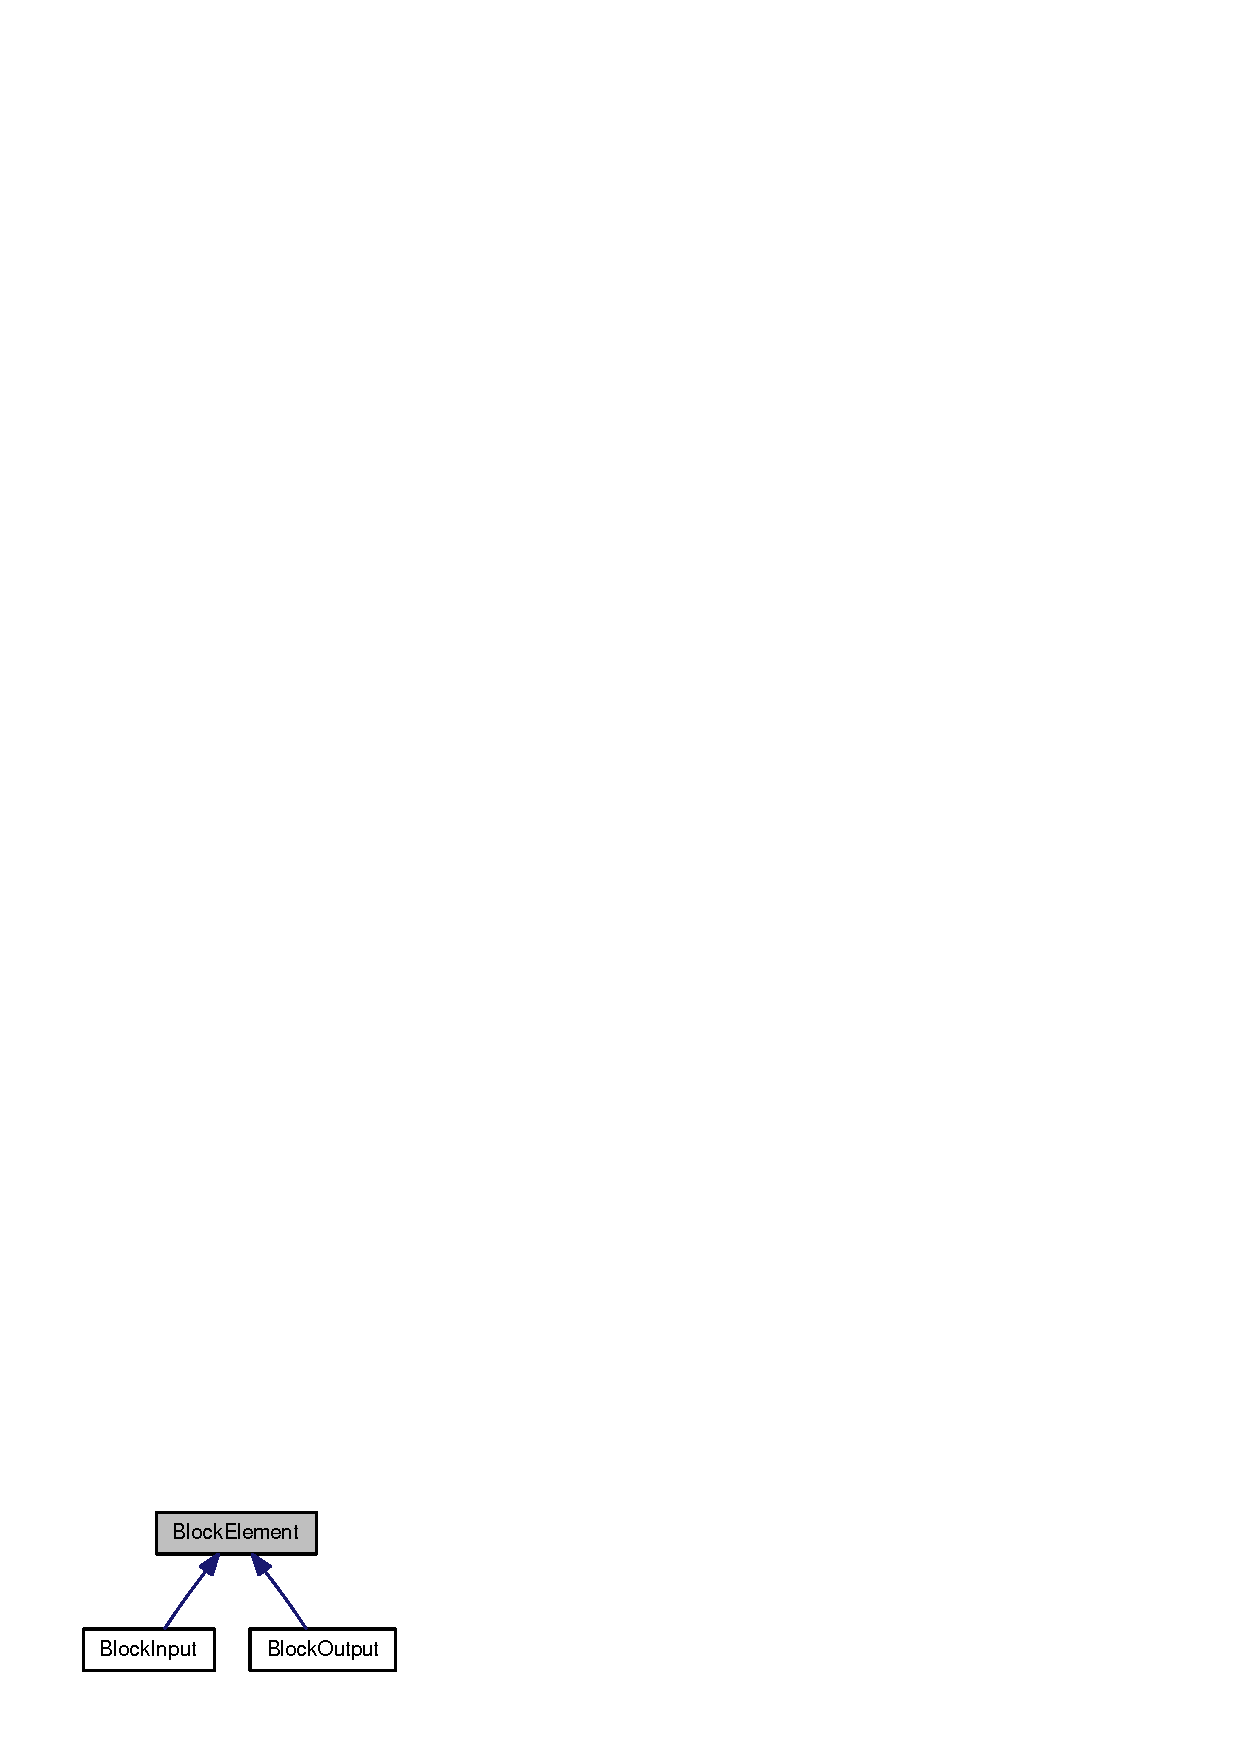
\includegraphics[width=97pt]{classBlockElement__inherit__graph}
\end{center}
\end{figure}
Collaboration diagram for BlockElement:\nopagebreak
\begin{figure}[H]
\begin{center}
\leavevmode
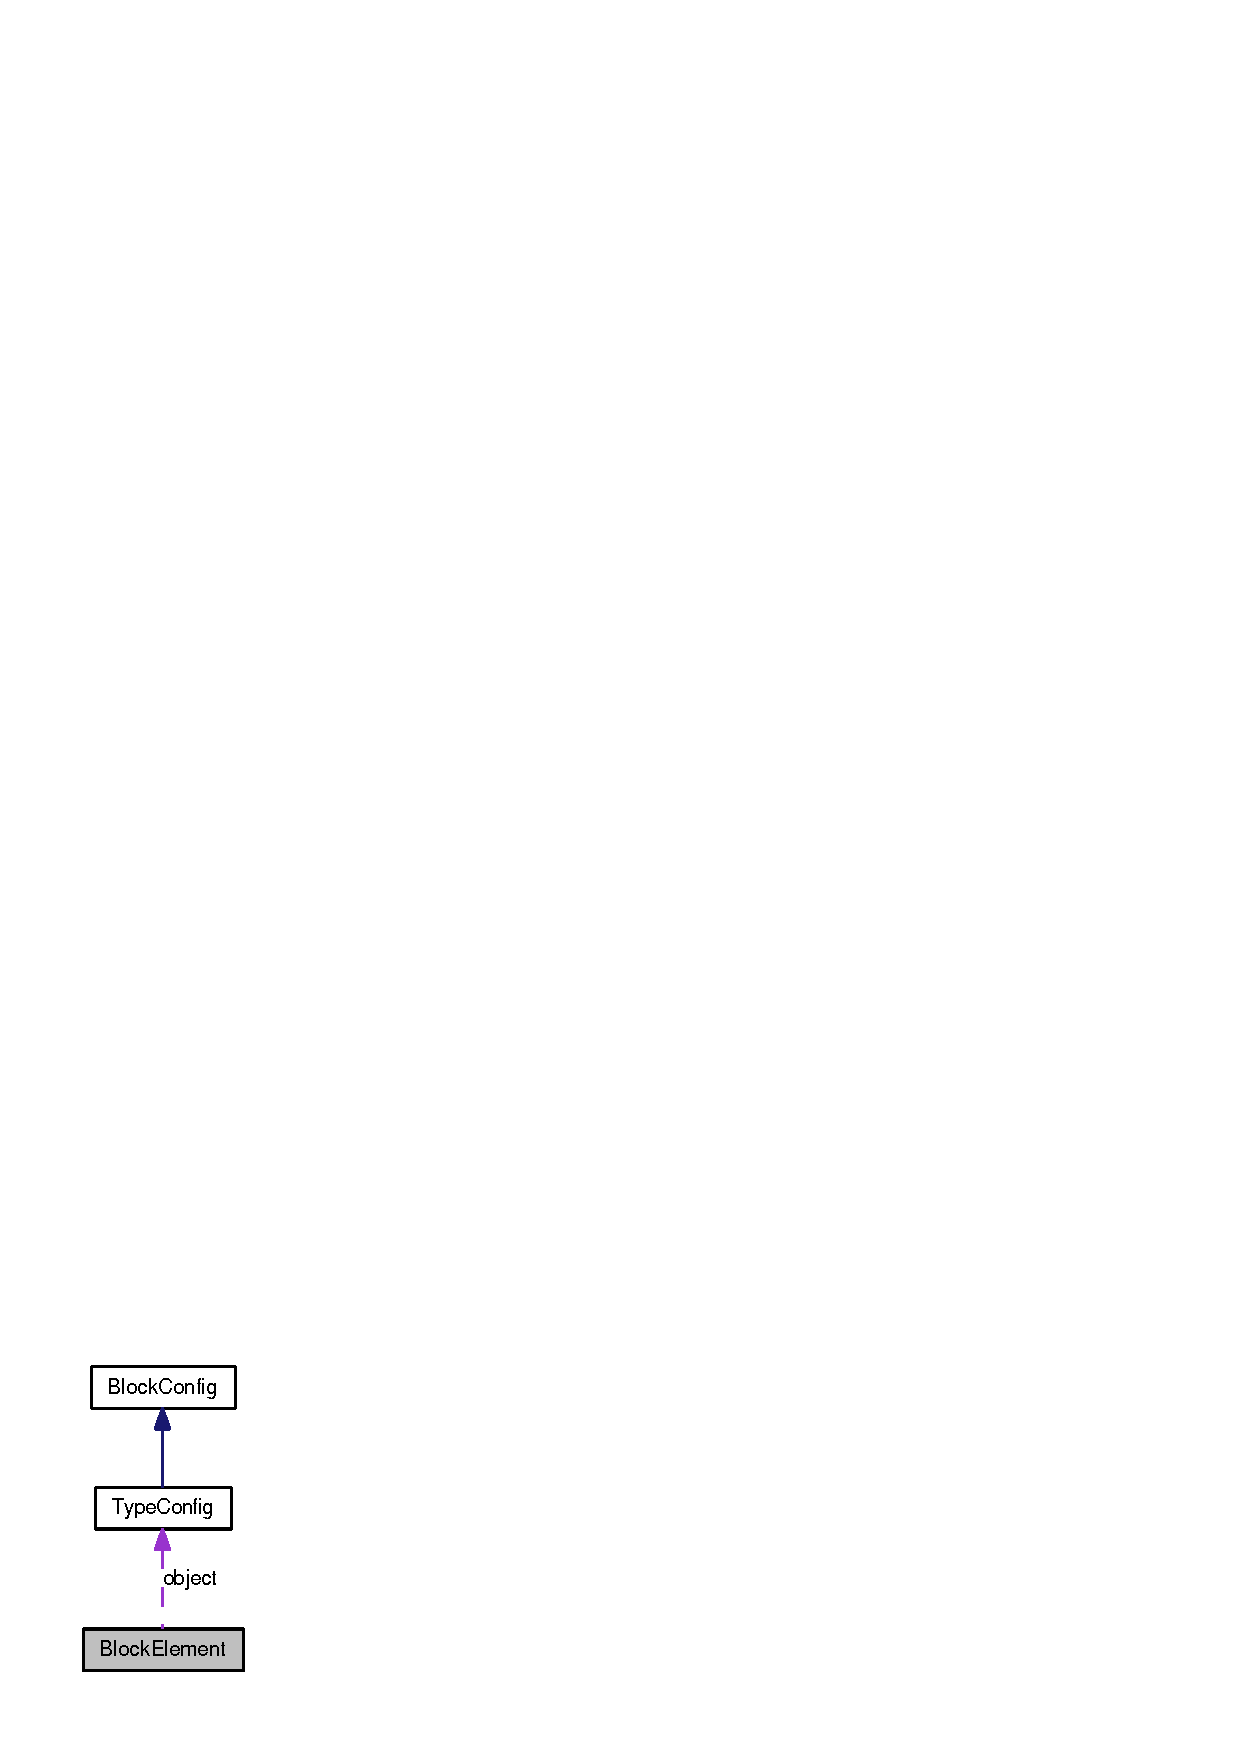
\includegraphics[width=60pt]{classBlockElement__coll__graph}
\end{center}
\end{figure}
\subsection*{Public Member Functions}
\begin{CompactItemize}
\item 
\hyperlink{classBlockElement_afefe31b25f85f8c35f5bbbcb525837a}{BlockElement} (const AnsiString aName)
\item 
\hyperlink{classBlockElement_e84bbdd297e6879e3650ce1117710ddf}{BlockElement} (const \hyperlink{classBlockElement}{BlockElement} \&block)
\item 
\hyperlink{classBlockElement_7cf305fa37661a18f4c1d4a37a58c365}{$\sim$BlockElement} ()
\item 
AnsiString \& \hyperlink{classBlockElement_2dd0f76d122144d9d6818ca0aad2b101}{getDescription} ()
\item 
int \hyperlink{classBlockElement_2dbc6e7c6ea9e27b11dcc3577880908f}{getErrorCode} ()
\item 
AnsiString \& \hyperlink{classBlockElement_a5956f89da9a3af217345cea3b9729d7}{getErrorDescription} ()
\item 
AnsiString \& \hyperlink{classBlockElement_353b53f27a0f60f380c557ceeef4aa31}{getName} ()
\item 
\hyperlink{classTypeConfig}{TypeConfig} $\ast$ \hyperlink{classBlockElement_6005a28d6f0ae61ce77c525b14b205c6}{getObject} ()
\item 
void \hyperlink{classBlockElement_2b9bb37f281555564978caf4b8658260}{setDescription} (const AnsiString aDescription)
\item 
void \hyperlink{classBlockElement_25fbc384ce7dae655edd1287d1d2a131}{setErrorDescription} (const AnsiString aErrorDescription)
\item 
void \hyperlink{classBlockElement_de2e8c4d1e423c27f833ef1b20752dc1}{setErrorCode} (int aError)
\item 
void \hyperlink{classBlockElement_0cf385c13d9044a097b1c7a2535b25b2}{setObject} (const \hyperlink{classTypeConfig}{TypeConfig} \&aData)
\item 
void \hyperlink{classBlockElement_6353263666225e0ed7a7e8942437234e}{clearObject} ()
\end{CompactItemize}
\subsection*{Protected Attributes}
\begin{CompactItemize}
\item 
AnsiString \hyperlink{classBlockElement_d0f7082fdc235d8aae07097dcdf64a2f}{description}
\item 
int \hyperlink{classBlockElement_bb7484a85df75f3dfe7e0646dc479c25}{errorCode}
\item 
AnsiString \hyperlink{classBlockElement_6d4cdaead6f246b33cab34eea19b339a}{errorDescription}
\item 
\hyperlink{classTypeConfig}{TypeConfig} $\ast$ \hyperlink{classBlockElement_20da3a345ba221325b61fd21f0f366b1}{object}
\item 
AnsiString \hyperlink{classBlockElement_dabe69719de30f09c4ffce479139c254}{name}
\end{CompactItemize}


\subsection{Detailed Description}
\hyperlink{classBlockElement}{BlockElement} - Klasa reprezentujaca wejscia/wyjscia miedzy blokami, zawiera - nazwe, opis, stan - czy jest poprawnie podlaczony (errorCode) \begin{Desc}
\item[Author:]Piotr \end{Desc}
\begin{Desc}
\item[Date:]2008.11.25 \end{Desc}
\begin{Desc}
\item[Version:]0.1 \end{Desc}


Definition at line 18 of file BlockElement.h.

\subsection{Constructor \& Destructor Documentation}
\hypertarget{classBlockElement_afefe31b25f85f8c35f5bbbcb525837a}{
\index{BlockElement@{BlockElement}!BlockElement@{BlockElement}}
\index{BlockElement@{BlockElement}!BlockElement@{BlockElement}}
\subsubsection[BlockElement]{\setlength{\rightskip}{0pt plus 5cm}BlockElement::BlockElement (const AnsiString {\em aName})}}
\label{classBlockElement_afefe31b25f85f8c35f5bbbcb525837a}


Konstruktor \begin{Desc}
\item[Parameters:]
\begin{description}
\item[{\em aName}]nazwa tworzonego wejscia/wyj�cia \end{description}
\end{Desc}


Definition at line 3 of file BlockElement.cpp.

References name.\hypertarget{classBlockElement_e84bbdd297e6879e3650ce1117710ddf}{
\index{BlockElement@{BlockElement}!BlockElement@{BlockElement}}
\index{BlockElement@{BlockElement}!BlockElement@{BlockElement}}
\subsubsection[BlockElement]{\setlength{\rightskip}{0pt plus 5cm}BlockElement::BlockElement (const {\bf BlockElement} \& {\em block})}}
\label{classBlockElement_e84bbdd297e6879e3650ce1117710ddf}


Konstruktor \begin{Desc}
\item[Parameters:]
\begin{description}
\item[{\em aName}]nazwa tworzonego wejscia/wyj�cia \end{description}
\end{Desc}


Definition at line 9 of file BlockElement.cpp.

References description, errorCode, errorDescription, name, and object.\hypertarget{classBlockElement_7cf305fa37661a18f4c1d4a37a58c365}{
\index{BlockElement@{BlockElement}!$\sim$BlockElement@{$\sim$BlockElement}}
\index{$\sim$BlockElement@{$\sim$BlockElement}!BlockElement@{BlockElement}}
\subsubsection[$\sim$BlockElement]{\setlength{\rightskip}{0pt plus 5cm}BlockElement::$\sim$BlockElement ()}}
\label{classBlockElement_7cf305fa37661a18f4c1d4a37a58c365}


Destruktor 

Definition at line 21 of file BlockElement.cpp.

References object.

\subsection{Member Function Documentation}
\hypertarget{classBlockElement_2dd0f76d122144d9d6818ca0aad2b101}{
\index{BlockElement@{BlockElement}!getDescription@{getDescription}}
\index{getDescription@{getDescription}!BlockElement@{BlockElement}}
\subsubsection[getDescription]{\setlength{\rightskip}{0pt plus 5cm}AnsiString \& BlockElement::getDescription ()}}
\label{classBlockElement_2dd0f76d122144d9d6818ca0aad2b101}


Pobiera opis. \begin{Desc}
\item[Returns:]AnsiString opis wejscia/wyj�cia. \end{Desc}


Definition at line 26 of file BlockElement.cpp.

References description.

Referenced by PIWOEngine::CancelCustomizationOnSelectedConnections(), PIWOEngine::DeleteSelectedConnection(), PIWOEngine::MakeConnection(), PIWOEngine::OnConnectionSelect(), PIWOEngine::OnVisualBlockInputHistoryClick(), PIWOEngine::OnVisualBlockInputSelected(), PIWOEngine::OnVisualBlockOutputHistoryClick(), PIWOEngine::OnVisualBlockOutputSelected(), PIWOEngine::UnselectSelectedConnection(), Connection::update(), and VisualBlock::updateVisualComponents().\hypertarget{classBlockElement_2dbc6e7c6ea9e27b11dcc3577880908f}{
\index{BlockElement@{BlockElement}!getErrorCode@{getErrorCode}}
\index{getErrorCode@{getErrorCode}!BlockElement@{BlockElement}}
\subsubsection[getErrorCode]{\setlength{\rightskip}{0pt plus 5cm}int BlockElement::getErrorCode ()}}
\label{classBlockElement_2dbc6e7c6ea9e27b11dcc3577880908f}


Pobiera kod bledu.  int kod bledu. 

Definition at line 31 of file BlockElement.cpp.

References errorCode.

Referenced by Connection::update(), VisualBlock::updateVisualComponents(), and PIWOEngine::validateBlock().\hypertarget{classBlockElement_a5956f89da9a3af217345cea3b9729d7}{
\index{BlockElement@{BlockElement}!getErrorDescription@{getErrorDescription}}
\index{getErrorDescription@{getErrorDescription}!BlockElement@{BlockElement}}
\subsubsection[getErrorDescription]{\setlength{\rightskip}{0pt plus 5cm}AnsiString \& BlockElement::getErrorDescription ()}}
\label{classBlockElement_a5956f89da9a3af217345cea3b9729d7}


Pobiera Opis bledu \begin{Desc}
\item[Returns:]AnsiString - Opis bledu. \end{Desc}


Definition at line 36 of file BlockElement.cpp.

References errorDescription.

Referenced by Connection::update(), VisualBlock::updateVisualComponents(), and PIWOEngine::validateBlock().\hypertarget{classBlockElement_353b53f27a0f60f380c557ceeef4aa31}{
\index{BlockElement@{BlockElement}!getName@{getName}}
\index{getName@{getName}!BlockElement@{BlockElement}}
\subsubsection[getName]{\setlength{\rightskip}{0pt plus 5cm}AnsiString \& BlockElement::getName ()}}
\label{classBlockElement_353b53f27a0f60f380c557ceeef4aa31}


Pobiera nazwe obiektu. \begin{Desc}
\item[Returns:]AnsiString nazwa obiektu. \end{Desc}


Definition at line 41 of file BlockElement.cpp.

References name.

Referenced by PIWOEngine::OnVisualBlockInputHistoryClick(), and PIWOEngine::OnVisualBlockOutputHistoryClick().\hypertarget{classBlockElement_6005a28d6f0ae61ce77c525b14b205c6}{
\index{BlockElement@{BlockElement}!getObject@{getObject}}
\index{getObject@{getObject}!BlockElement@{BlockElement}}
\subsubsection[getObject]{\setlength{\rightskip}{0pt plus 5cm}{\bf TypeConfig} $\ast$ BlockElement::getObject ()}}
\label{classBlockElement_6005a28d6f0ae61ce77c525b14b205c6}


Pobiera Konfiguracje bloku. \begin{Desc}
\item[Returns:]\hyperlink{classTypeConfig}{TypeConfig} konfiguracja bloku. \end{Desc}


Definition at line 46 of file BlockElement.cpp.

References object.

Referenced by PIWOEngine::runBlock().\hypertarget{classBlockElement_2b9bb37f281555564978caf4b8658260}{
\index{BlockElement@{BlockElement}!setDescription@{setDescription}}
\index{setDescription@{setDescription}!BlockElement@{BlockElement}}
\subsubsection[setDescription]{\setlength{\rightskip}{0pt plus 5cm}void BlockElement::setDescription (const AnsiString {\em aDescription})}}
\label{classBlockElement_2b9bb37f281555564978caf4b8658260}


Ustawia opis. \begin{Desc}
\item[Parameters:]
\begin{description}
\item[{\em aDescription}]- ustawiany opis. \end{description}
\end{Desc}


Definition at line 51 of file BlockElement.cpp.

References description.

Referenced by PIWOEngine::loadFromFile().\hypertarget{classBlockElement_25fbc384ce7dae655edd1287d1d2a131}{
\index{BlockElement@{BlockElement}!setErrorDescription@{setErrorDescription}}
\index{setErrorDescription@{setErrorDescription}!BlockElement@{BlockElement}}
\subsubsection[setErrorDescription]{\setlength{\rightskip}{0pt plus 5cm}void BlockElement::setErrorDescription (const AnsiString {\em aErrorDescription})}}
\label{classBlockElement_25fbc384ce7dae655edd1287d1d2a131}


Ustawia opis bledu. \begin{Desc}
\item[Parameters:]
\begin{description}
\item[{\em aErrorDescription}]- ustawiany opis bledu. \end{description}
\end{Desc}


Definition at line 56 of file BlockElement.cpp.

References errorDescription.

Referenced by PIWOEngine::loadFromFile().\hypertarget{classBlockElement_de2e8c4d1e423c27f833ef1b20752dc1}{
\index{BlockElement@{BlockElement}!setErrorCode@{setErrorCode}}
\index{setErrorCode@{setErrorCode}!BlockElement@{BlockElement}}
\subsubsection[setErrorCode]{\setlength{\rightskip}{0pt plus 5cm}void BlockElement::setErrorCode (int {\em aError})}}
\label{classBlockElement_de2e8c4d1e423c27f833ef1b20752dc1}


Ustawia kod blad. \begin{Desc}
\item[Parameters:]
\begin{description}
\item[{\em aError}]- ustawiany kod,0-ok, 1-warrning, 2-error. \end{description}
\end{Desc}


Definition at line 61 of file BlockElement.cpp.

References errorCode.

Referenced by PIWOEngine::loadFromFile().\hypertarget{classBlockElement_0cf385c13d9044a097b1c7a2535b25b2}{
\index{BlockElement@{BlockElement}!setObject@{setObject}}
\index{setObject@{setObject}!BlockElement@{BlockElement}}
\subsubsection[setObject]{\setlength{\rightskip}{0pt plus 5cm}void BlockElement::setObject (const {\bf TypeConfig} \& {\em aData})}}
\label{classBlockElement_0cf385c13d9044a097b1c7a2535b25b2}


Ustawia obiekt. \begin{Desc}
\item[Parameters:]
\begin{description}
\item[{\em aData}]- ustawiany obiekt. \end{description}
\end{Desc}


Definition at line 66 of file BlockElement.cpp.

References object.\hypertarget{classBlockElement_6353263666225e0ed7a7e8942437234e}{
\index{BlockElement@{BlockElement}!clearObject@{clearObject}}
\index{clearObject@{clearObject}!BlockElement@{BlockElement}}
\subsubsection[clearObject]{\setlength{\rightskip}{0pt plus 5cm}void BlockElement::clearObject ()}}
\label{classBlockElement_6353263666225e0ed7a7e8942437234e}


Usuwa obiekt. 

Definition at line 72 of file BlockElement.cpp.

References object.

\subsection{Member Data Documentation}
\hypertarget{classBlockElement_d0f7082fdc235d8aae07097dcdf64a2f}{
\index{BlockElement@{BlockElement}!description@{description}}
\index{description@{description}!BlockElement@{BlockElement}}
\subsubsection[description]{\setlength{\rightskip}{0pt plus 5cm}AnsiString {\bf BlockElement::description}\hspace{0.3cm}{\tt  \mbox{[}protected\mbox{]}}}}
\label{classBlockElement_d0f7082fdc235d8aae07097dcdf64a2f}




Definition at line 21 of file BlockElement.h.

Referenced by BlockElement(), getDescription(), and setDescription().\hypertarget{classBlockElement_bb7484a85df75f3dfe7e0646dc479c25}{
\index{BlockElement@{BlockElement}!errorCode@{errorCode}}
\index{errorCode@{errorCode}!BlockElement@{BlockElement}}
\subsubsection[errorCode]{\setlength{\rightskip}{0pt plus 5cm}int {\bf BlockElement::errorCode}\hspace{0.3cm}{\tt  \mbox{[}protected\mbox{]}}}}
\label{classBlockElement_bb7484a85df75f3dfe7e0646dc479c25}




Definition at line 22 of file BlockElement.h.

Referenced by BlockElement(), getErrorCode(), and setErrorCode().\hypertarget{classBlockElement_6d4cdaead6f246b33cab34eea19b339a}{
\index{BlockElement@{BlockElement}!errorDescription@{errorDescription}}
\index{errorDescription@{errorDescription}!BlockElement@{BlockElement}}
\subsubsection[errorDescription]{\setlength{\rightskip}{0pt plus 5cm}AnsiString {\bf BlockElement::errorDescription}\hspace{0.3cm}{\tt  \mbox{[}protected\mbox{]}}}}
\label{classBlockElement_6d4cdaead6f246b33cab34eea19b339a}




Definition at line 23 of file BlockElement.h.

Referenced by BlockElement(), getErrorDescription(), and setErrorDescription().\hypertarget{classBlockElement_20da3a345ba221325b61fd21f0f366b1}{
\index{BlockElement@{BlockElement}!object@{object}}
\index{object@{object}!BlockElement@{BlockElement}}
\subsubsection[object]{\setlength{\rightskip}{0pt plus 5cm}{\bf TypeConfig}$\ast$ {\bf BlockElement::object}\hspace{0.3cm}{\tt  \mbox{[}protected\mbox{]}}}}
\label{classBlockElement_20da3a345ba221325b61fd21f0f366b1}




Definition at line 24 of file BlockElement.h.

Referenced by BlockElement(), clearObject(), getObject(), setObject(), and $\sim$BlockElement().\hypertarget{classBlockElement_dabe69719de30f09c4ffce479139c254}{
\index{BlockElement@{BlockElement}!name@{name}}
\index{name@{name}!BlockElement@{BlockElement}}
\subsubsection[name]{\setlength{\rightskip}{0pt plus 5cm}AnsiString {\bf BlockElement::name}\hspace{0.3cm}{\tt  \mbox{[}protected\mbox{]}}}}
\label{classBlockElement_dabe69719de30f09c4ffce479139c254}




Definition at line 25 of file BlockElement.h.

Referenced by BlockElement(), and getName().

The documentation for this class was generated from the following files:\begin{CompactItemize}
\item 
/PIWO/Program/engine/\hyperlink{BlockElement_8h}{BlockElement.h}\item 
/PIWO/Program/engine/\hyperlink{BlockElement_8cpp}{BlockElement.cpp}\end{CompactItemize}

\hypertarget{classBlockHistory}{
\section{BlockHistory Class Reference}
\label{classBlockHistory}\index{BlockHistory@{BlockHistory}}
}
{\tt \#include $<$BlockHistory.h$>$}

\subsection*{Public Member Functions}
\begin{CompactItemize}
\item 
\hyperlink{classBlockHistory_c489ea0976659cf022e67ef750162313}{BlockHistory} ()
\item 
\hyperlink{classBlockHistory_26fc96f5239718c5866d2682161c1800}{BlockHistory} (\hyperlink{classBlockHistory}{BlockHistory} \&b)
\item 
\hyperlink{classBlockHistory_0647b0c5491b4755250ee1e0d5cb9a8f}{$\sim$BlockHistory} ()
\end{CompactItemize}
\subsection*{Public Attributes}
\begin{CompactItemize}
\item 
vector$<$ \hyperlink{classBlockHistoryInputElement}{BlockHistoryInputElement} $\ast$ $>$ \hyperlink{classBlockHistory_aabd8ceb5c5cf94ca36778ad9a703c79}{leftInput}
\item 
vector$<$ \hyperlink{classBlockHistoryInputElement}{BlockHistoryInputElement} $\ast$ $>$ \hyperlink{classBlockHistory_206bee2db6d12c0d406d90d3dc4b54ac}{topInput}
\item 
vector$<$ \hyperlink{classBlockHistoryOutputElement}{BlockHistoryOutputElement} $\ast$ $>$ \hyperlink{classBlockHistory_e7d44768a04aeb3d73444ec684486f08}{rightOutput}
\item 
vector$<$ \hyperlink{classBlockHistoryOutputElement}{BlockHistoryOutputElement} $\ast$ $>$ \hyperlink{classBlockHistory_d6bac65bd73326840162bbb9cd8d14c1}{bottomOutput}
\item 
unsigned int \hyperlink{classBlockHistory_a491be49ba9d081df6d1213481346ea9}{configRevision}
\item 
TDateTime \hyperlink{classBlockHistory_0b1d6f43a3ba643ad8f387f7c9f2abc7}{date}
\end{CompactItemize}


\subsection{Detailed Description}
Klasa zawiera historie dla calego bloku po jego jednokrotnym uruchomieniu. 

Definition at line 10 of file BlockHistory.h.

\subsection{Constructor \& Destructor Documentation}
\hypertarget{classBlockHistory_c489ea0976659cf022e67ef750162313}{
\index{BlockHistory@{BlockHistory}!BlockHistory@{BlockHistory}}
\index{BlockHistory@{BlockHistory}!BlockHistory@{BlockHistory}}
\subsubsection[BlockHistory]{\setlength{\rightskip}{0pt plus 5cm}BlockHistory::BlockHistory ()}}
\label{classBlockHistory_c489ea0976659cf022e67ef750162313}


Konstruktor domyslny 

Definition at line 6 of file BlockHistory.cpp.

References configRevision, and date.\hypertarget{classBlockHistory_26fc96f5239718c5866d2682161c1800}{
\index{BlockHistory@{BlockHistory}!BlockHistory@{BlockHistory}}
\index{BlockHistory@{BlockHistory}!BlockHistory@{BlockHistory}}
\subsubsection[BlockHistory]{\setlength{\rightskip}{0pt plus 5cm}BlockHistory::BlockHistory ({\bf BlockHistory} \& {\em b})}}
\label{classBlockHistory_26fc96f5239718c5866d2682161c1800}


Konstruktor kopiujacy \begin{Desc}
\item[Parameters:]
\begin{description}
\item[{\em ob}]obiekt z ktorego mamy skopiowac \end{description}
\end{Desc}


Definition at line 12 of file BlockHistory.cpp.

References bottomOutput, configRevision, date, leftInput, rightOutput, and topInput.\hypertarget{classBlockHistory_0647b0c5491b4755250ee1e0d5cb9a8f}{
\index{BlockHistory@{BlockHistory}!$\sim$BlockHistory@{$\sim$BlockHistory}}
\index{$\sim$BlockHistory@{$\sim$BlockHistory}!BlockHistory@{BlockHistory}}
\subsubsection[$\sim$BlockHistory]{\setlength{\rightskip}{0pt plus 5cm}BlockHistory::$\sim$BlockHistory ()}}
\label{classBlockHistory_0647b0c5491b4755250ee1e0d5cb9a8f}


Destruktor 

Definition at line 22 of file BlockHistory.cpp.

References bottomOutput, leftInput, rightOutput, and topInput.

\subsection{Member Data Documentation}
\hypertarget{classBlockHistory_aabd8ceb5c5cf94ca36778ad9a703c79}{
\index{BlockHistory@{BlockHistory}!leftInput@{leftInput}}
\index{leftInput@{leftInput}!BlockHistory@{BlockHistory}}
\subsubsection[leftInput]{\setlength{\rightskip}{0pt plus 5cm}vector$<${\bf BlockHistoryInputElement}$\ast$$>$ {\bf BlockHistory::leftInput}}}
\label{classBlockHistory_aabd8ceb5c5cf94ca36778ad9a703c79}


Lista histori dla wejsc z lewej strony bloczka 

Definition at line 16 of file BlockHistory.h.

Referenced by BlockHistory(), PIWOEngine::runBlock(), and $\sim$BlockHistory().\hypertarget{classBlockHistory_206bee2db6d12c0d406d90d3dc4b54ac}{
\index{BlockHistory@{BlockHistory}!topInput@{topInput}}
\index{topInput@{topInput}!BlockHistory@{BlockHistory}}
\subsubsection[topInput]{\setlength{\rightskip}{0pt plus 5cm}vector$<${\bf BlockHistoryInputElement}$\ast$$>$ {\bf BlockHistory::topInput}}}
\label{classBlockHistory_206bee2db6d12c0d406d90d3dc4b54ac}


Lista histori dla wejsc z gornej strony bloczka 

Definition at line 20 of file BlockHistory.h.

Referenced by BlockHistory(), PIWOEngine::runBlock(), and $\sim$BlockHistory().\hypertarget{classBlockHistory_e7d44768a04aeb3d73444ec684486f08}{
\index{BlockHistory@{BlockHistory}!rightOutput@{rightOutput}}
\index{rightOutput@{rightOutput}!BlockHistory@{BlockHistory}}
\subsubsection[rightOutput]{\setlength{\rightskip}{0pt plus 5cm}vector$<${\bf BlockHistoryOutputElement}$\ast$$>$ {\bf BlockHistory::rightOutput}}}
\label{classBlockHistory_e7d44768a04aeb3d73444ec684486f08}


Lista histori dla wyjsc z prawej strony bloczka 

Definition at line 24 of file BlockHistory.h.

Referenced by BlockHistory(), PIWOEngine::runBlock(), and $\sim$BlockHistory().\hypertarget{classBlockHistory_d6bac65bd73326840162bbb9cd8d14c1}{
\index{BlockHistory@{BlockHistory}!bottomOutput@{bottomOutput}}
\index{bottomOutput@{bottomOutput}!BlockHistory@{BlockHistory}}
\subsubsection[bottomOutput]{\setlength{\rightskip}{0pt plus 5cm}vector$<${\bf BlockHistoryOutputElement}$\ast$$>$ {\bf BlockHistory::bottomOutput}}}
\label{classBlockHistory_d6bac65bd73326840162bbb9cd8d14c1}


Lista histori dla wyjsc z dolnej strony bloczka 

Definition at line 28 of file BlockHistory.h.

Referenced by BlockHistory(), PIWOEngine::runBlock(), and $\sim$BlockHistory().\hypertarget{classBlockHistory_a491be49ba9d081df6d1213481346ea9}{
\index{BlockHistory@{BlockHistory}!configRevision@{configRevision}}
\index{configRevision@{configRevision}!BlockHistory@{BlockHistory}}
\subsubsection[configRevision]{\setlength{\rightskip}{0pt plus 5cm}unsigned int {\bf BlockHistory::configRevision}}}
\label{classBlockHistory_a491be49ba9d081df6d1213481346ea9}


Wersja konfiguracji 

Definition at line 32 of file BlockHistory.h.

Referenced by BlockHistory(), and PIWOEngine::runBlock().\hypertarget{classBlockHistory_0b1d6f43a3ba643ad8f387f7c9f2abc7}{
\index{BlockHistory@{BlockHistory}!date@{date}}
\index{date@{date}!BlockHistory@{BlockHistory}}
\subsubsection[date]{\setlength{\rightskip}{0pt plus 5cm}TDateTime {\bf BlockHistory::date}}}
\label{classBlockHistory_0b1d6f43a3ba643ad8f387f7c9f2abc7}


Data i godzina dodania histori 

Definition at line 36 of file BlockHistory.h.

Referenced by BlockHistory().

The documentation for this class was generated from the following files:\begin{CompactItemize}
\item 
/PIWO/Program/gui/\hyperlink{BlockHistory_8h}{BlockHistory.h}\item 
/PIWO/Program/gui/\hyperlink{BlockHistory_8cpp}{BlockHistory.cpp}\end{CompactItemize}

\hypertarget{classBlockHistoryInputElement}{
\section{BlockHistoryInputElement Class Reference}
\label{classBlockHistoryInputElement}\index{BlockHistoryInputElement@{BlockHistoryInputElement}}
}
{\tt \#include $<$BlockHistoryInputElement.h$>$}

Collaboration diagram for BlockHistoryInputElement:\nopagebreak
\begin{figure}[H]
\begin{center}
\leavevmode
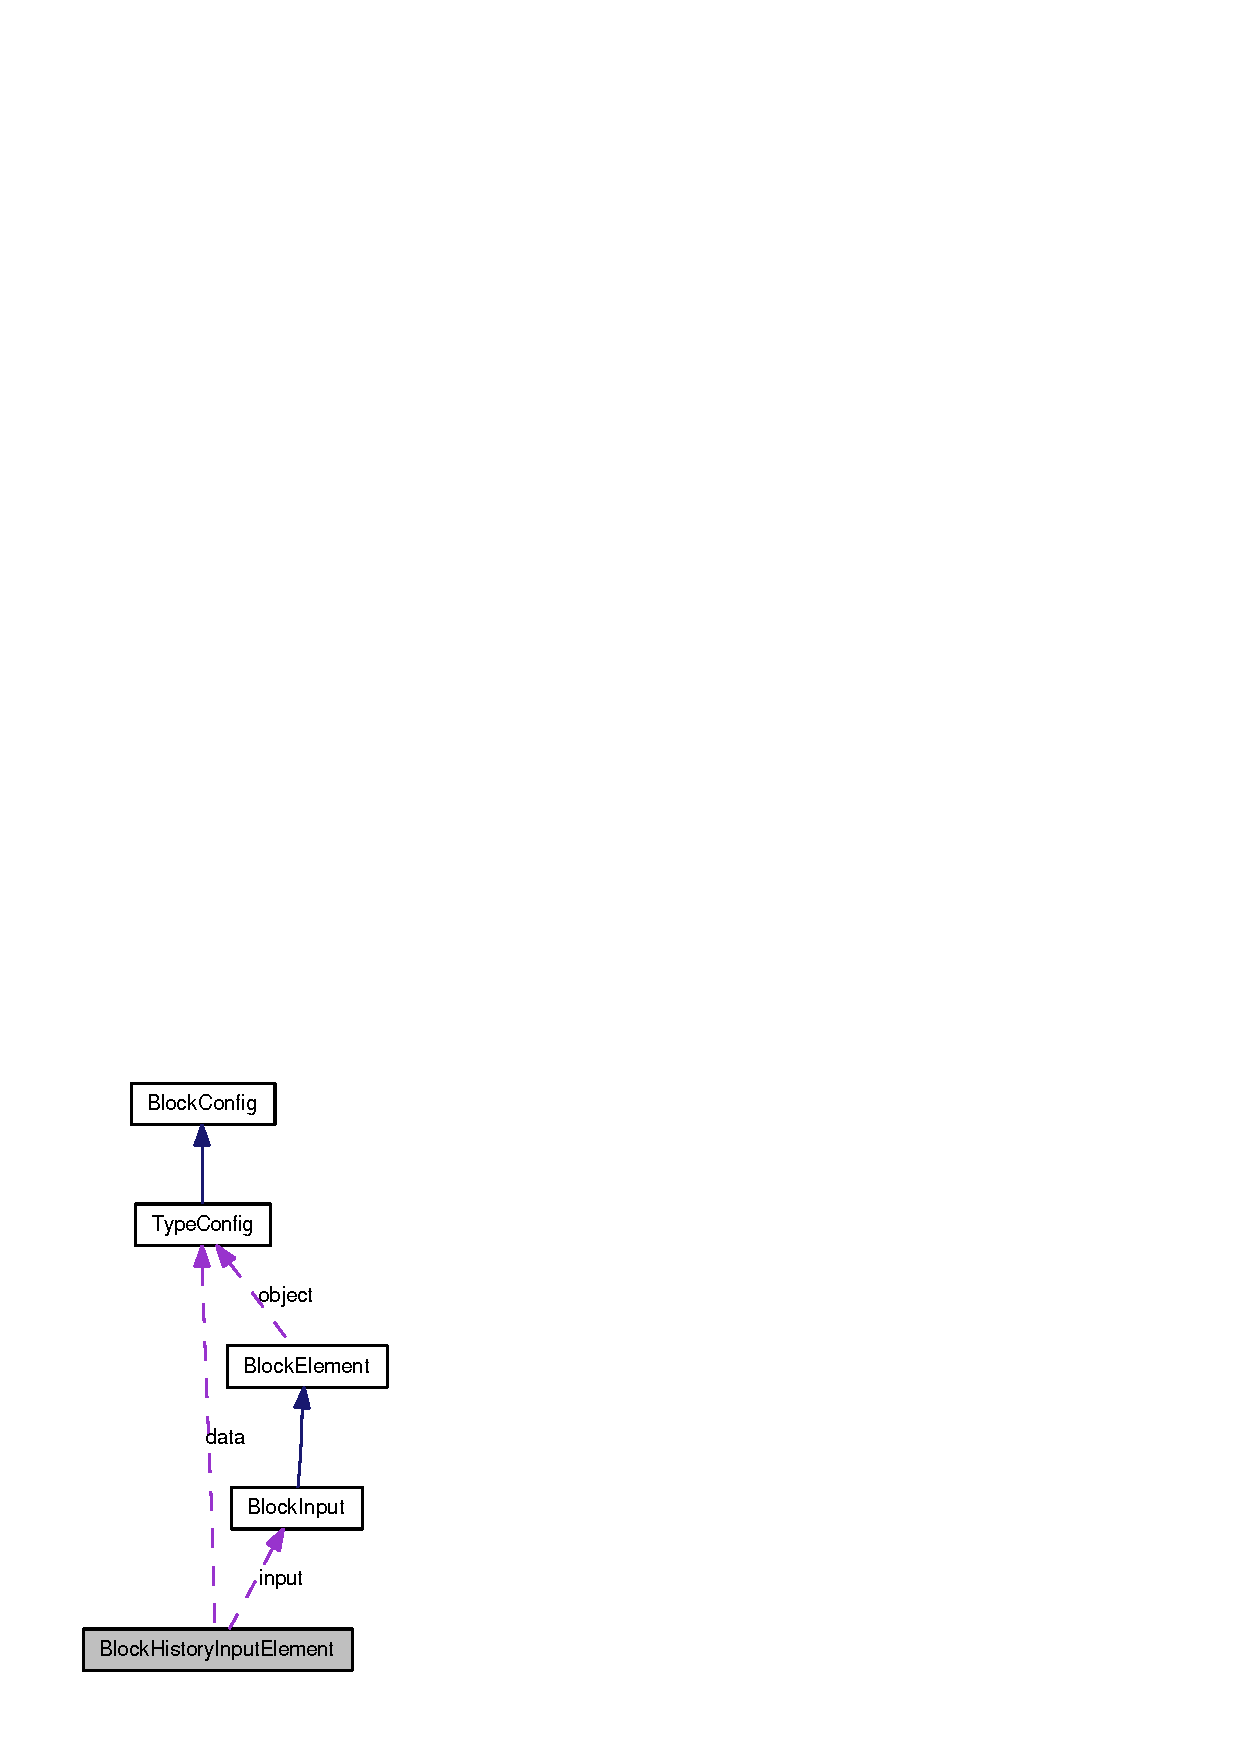
\includegraphics[width=94pt]{classBlockHistoryInputElement__coll__graph}
\end{center}
\end{figure}
\subsection*{Public Member Functions}
\begin{CompactItemize}
\item 
void \hyperlink{classBlockHistoryInputElement_4a8ebf161f64bbb97cf8b694cd6a72bf}{setData} (\hyperlink{classTypeConfig}{TypeConfig} \&d)
\item 
void \hyperlink{classBlockHistoryInputElement_a3c4c677fcb9c0dbb8f3e31314627ca1}{setNULL} ()
\item 
\hyperlink{classTypeConfig}{TypeConfig} $\ast$ \hyperlink{classBlockHistoryInputElement_d980299844b1b410df13ef28502c73fd}{getData} ()
\item 
\hyperlink{classBlockHistoryInputElement_40ce1d8e1e4f6e7654e31e7dff51bb42}{BlockHistoryInputElement} ()
\item 
\hyperlink{classBlockHistoryInputElement_122c02aac40c5b3e7ff7935e68f36469}{$\sim$BlockHistoryInputElement} ()
\end{CompactItemize}
\subsection*{Public Attributes}
\begin{CompactItemize}
\item 
\hyperlink{classBlockInput}{BlockInput} $\ast$ \hyperlink{classBlockHistoryInputElement_5a307d34d5e47b9baf161c7069415c93}{input}
\end{CompactItemize}
\subsection*{Private Attributes}
\begin{CompactItemize}
\item 
\hyperlink{classTypeConfig}{TypeConfig} $\ast$ \hyperlink{classBlockHistoryInputElement_e8c6facba5335a07f2452279191cd6e8}{data}
\end{CompactItemize}


\subsection{Detailed Description}
Klasa zawiera historie dla pojedynczego wejscia bloku 

Definition at line 9 of file BlockHistoryInputElement.h.

\subsection{Constructor \& Destructor Documentation}
\hypertarget{classBlockHistoryInputElement_40ce1d8e1e4f6e7654e31e7dff51bb42}{
\index{BlockHistoryInputElement@{BlockHistoryInputElement}!BlockHistoryInputElement@{BlockHistoryInputElement}}
\index{BlockHistoryInputElement@{BlockHistoryInputElement}!BlockHistoryInputElement@{BlockHistoryInputElement}}
\subsubsection[BlockHistoryInputElement]{\setlength{\rightskip}{0pt plus 5cm}BlockHistoryInputElement::BlockHistoryInputElement ()}}
\label{classBlockHistoryInputElement_40ce1d8e1e4f6e7654e31e7dff51bb42}


Konstruktor 

Definition at line 6 of file BlockHistoryInputElement.cpp.

References data, and input.\hypertarget{classBlockHistoryInputElement_122c02aac40c5b3e7ff7935e68f36469}{
\index{BlockHistoryInputElement@{BlockHistoryInputElement}!$\sim$BlockHistoryInputElement@{$\sim$BlockHistoryInputElement}}
\index{$\sim$BlockHistoryInputElement@{$\sim$BlockHistoryInputElement}!BlockHistoryInputElement@{BlockHistoryInputElement}}
\subsubsection[$\sim$BlockHistoryInputElement]{\setlength{\rightskip}{0pt plus 5cm}BlockHistoryInputElement::$\sim$BlockHistoryInputElement ()}}
\label{classBlockHistoryInputElement_122c02aac40c5b3e7ff7935e68f36469}


Destruktor 

Definition at line 12 of file BlockHistoryInputElement.cpp.

References data.

\subsection{Member Function Documentation}
\hypertarget{classBlockHistoryInputElement_4a8ebf161f64bbb97cf8b694cd6a72bf}{
\index{BlockHistoryInputElement@{BlockHistoryInputElement}!setData@{setData}}
\index{setData@{setData}!BlockHistoryInputElement@{BlockHistoryInputElement}}
\subsubsection[setData]{\setlength{\rightskip}{0pt plus 5cm}void BlockHistoryInputElement::setData ({\bf TypeConfig} \& {\em d})}}
\label{classBlockHistoryInputElement_4a8ebf161f64bbb97cf8b694cd6a72bf}


Ustawia obiekt \begin{Desc}
\item[Parameters:]
\begin{description}
\item[{\em d}]dane \end{description}
\end{Desc}


Definition at line 17 of file BlockHistoryInputElement.cpp.

References data.

Referenced by PIWOEngine::runBlock().\hypertarget{classBlockHistoryInputElement_a3c4c677fcb9c0dbb8f3e31314627ca1}{
\index{BlockHistoryInputElement@{BlockHistoryInputElement}!setNULL@{setNULL}}
\index{setNULL@{setNULL}!BlockHistoryInputElement@{BlockHistoryInputElement}}
\subsubsection[setNULL]{\setlength{\rightskip}{0pt plus 5cm}void BlockHistoryInputElement::setNULL ()}}
\label{classBlockHistoryInputElement_a3c4c677fcb9c0dbb8f3e31314627ca1}


Czysci obiekt 

Definition at line 28 of file BlockHistoryInputElement.cpp.

References data.

Referenced by PIWOEngine::runBlock().\hypertarget{classBlockHistoryInputElement_d980299844b1b410df13ef28502c73fd}{
\index{BlockHistoryInputElement@{BlockHistoryInputElement}!getData@{getData}}
\index{getData@{getData}!BlockHistoryInputElement@{BlockHistoryInputElement}}
\subsubsection[getData]{\setlength{\rightskip}{0pt plus 5cm}{\bf TypeConfig} $\ast$ BlockHistoryInputElement::getData ()}}
\label{classBlockHistoryInputElement_d980299844b1b410df13ef28502c73fd}


Zwraca obiekt \begin{Desc}
\item[Returns:]NULL lub TypeConfig$\ast$ \end{Desc}


Definition at line 23 of file BlockHistoryInputElement.cpp.

References data.

\subsection{Member Data Documentation}
\hypertarget{classBlockHistoryInputElement_e8c6facba5335a07f2452279191cd6e8}{
\index{BlockHistoryInputElement@{BlockHistoryInputElement}!data@{data}}
\index{data@{data}!BlockHistoryInputElement@{BlockHistoryInputElement}}
\subsubsection[data]{\setlength{\rightskip}{0pt plus 5cm}{\bf TypeConfig}$\ast$ {\bf BlockHistoryInputElement::data}\hspace{0.3cm}{\tt  \mbox{[}private\mbox{]}}}}
\label{classBlockHistoryInputElement_e8c6facba5335a07f2452279191cd6e8}




Definition at line 12 of file BlockHistoryInputElement.h.

Referenced by BlockHistoryInputElement(), getData(), setData(), setNULL(), and $\sim$BlockHistoryInputElement().\hypertarget{classBlockHistoryInputElement_5a307d34d5e47b9baf161c7069415c93}{
\index{BlockHistoryInputElement@{BlockHistoryInputElement}!input@{input}}
\index{input@{input}!BlockHistoryInputElement@{BlockHistoryInputElement}}
\subsubsection[input]{\setlength{\rightskip}{0pt plus 5cm}{\bf BlockInput}$\ast$ {\bf BlockHistoryInputElement::input}}}
\label{classBlockHistoryInputElement_5a307d34d5e47b9baf161c7069415c93}


Wejscie bloku 

Definition at line 17 of file BlockHistoryInputElement.h.

Referenced by BlockHistoryInputElement(), and PIWOEngine::runBlock().

The documentation for this class was generated from the following files:\begin{CompactItemize}
\item 
/PIWO/Program/gui/\hyperlink{BlockHistoryInputElement_8h}{BlockHistoryInputElement.h}\item 
/PIWO/Program/gui/\hyperlink{BlockHistoryInputElement_8cpp}{BlockHistoryInputElement.cpp}\end{CompactItemize}

\hypertarget{classBlockHistoryOutputElement}{
\section{BlockHistoryOutputElement Class Reference}
\label{classBlockHistoryOutputElement}\index{BlockHistoryOutputElement@{BlockHistoryOutputElement}}
}
{\tt \#include $<$BlockHistoryOutputElement.h$>$}

Collaboration diagram for BlockHistoryOutputElement:\nopagebreak
\begin{figure}[H]
\begin{center}
\leavevmode
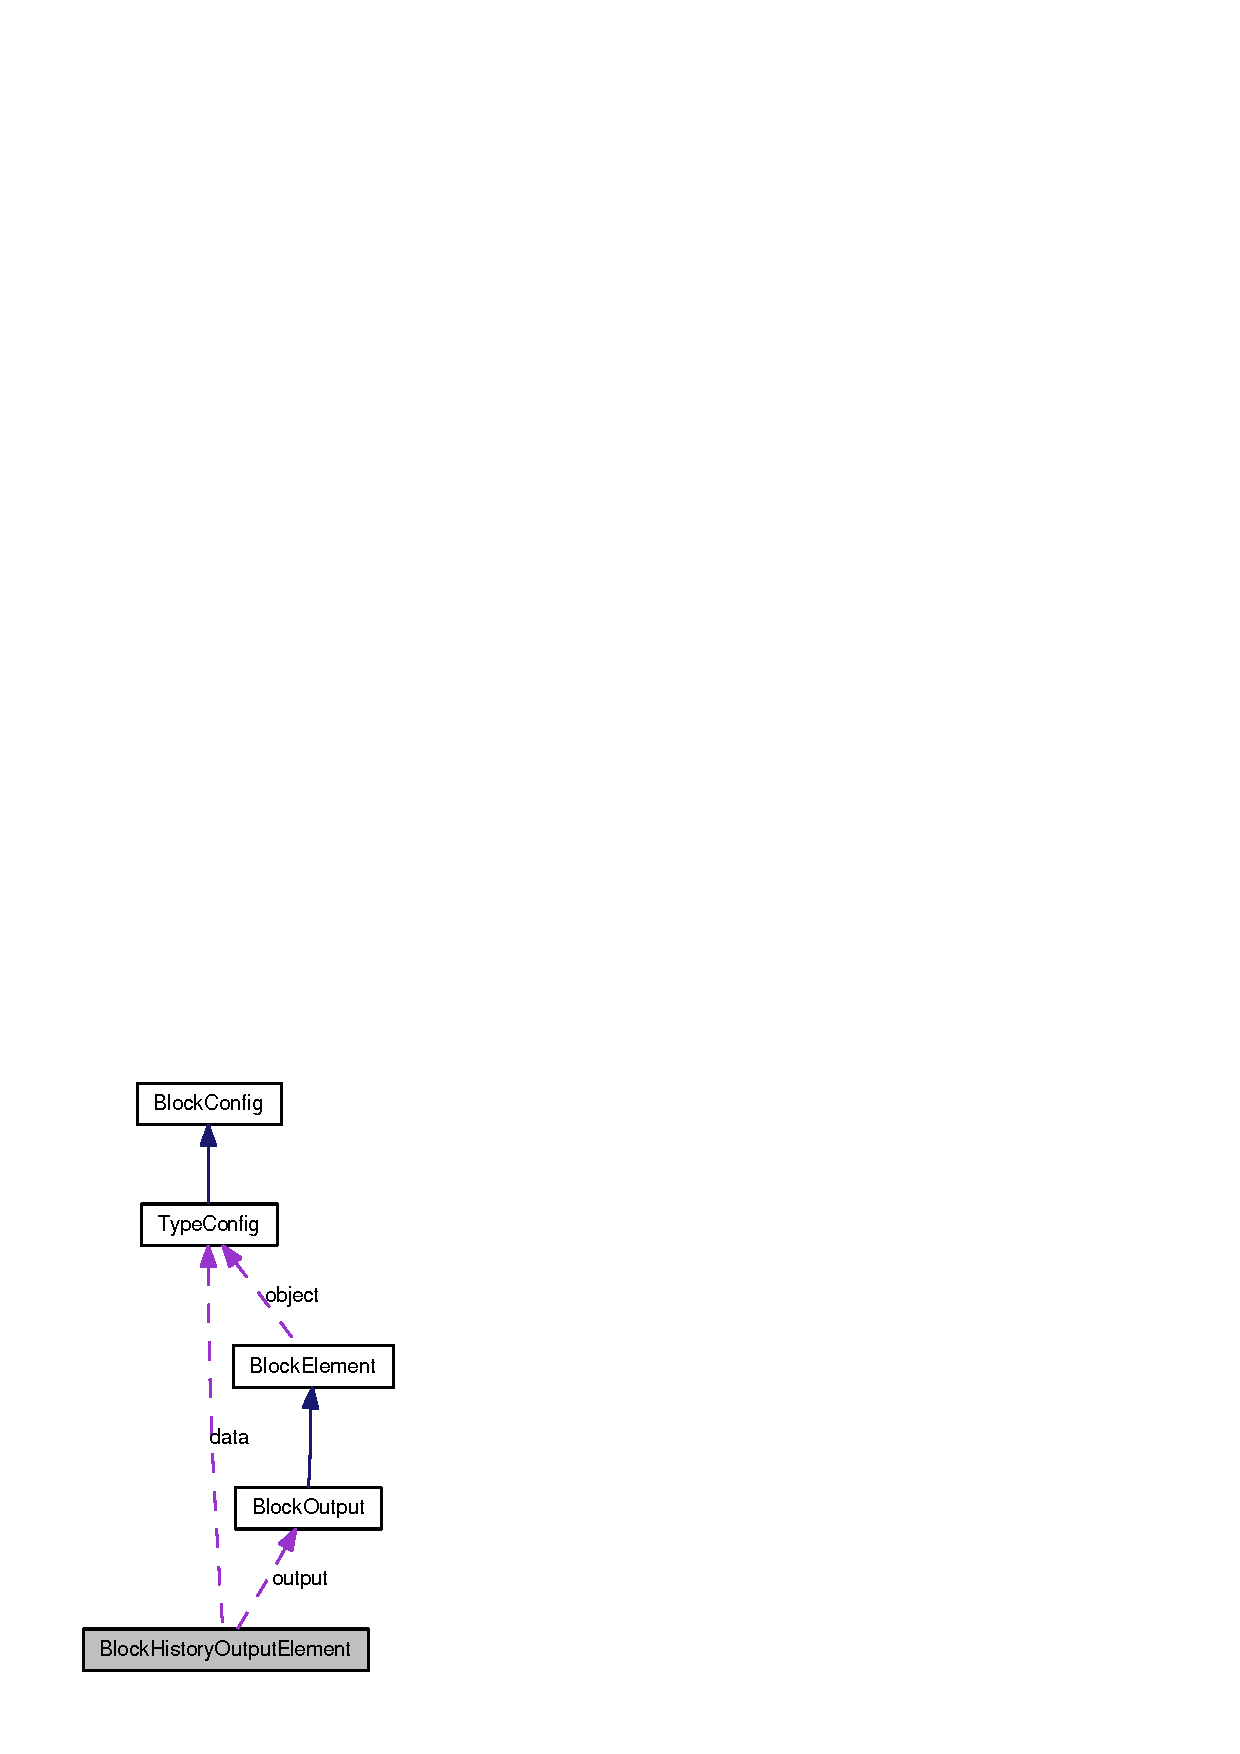
\includegraphics[width=96pt]{classBlockHistoryOutputElement__coll__graph}
\end{center}
\end{figure}
\subsection*{Public Member Functions}
\begin{CompactItemize}
\item 
void \hyperlink{classBlockHistoryOutputElement_c6a108725145c059f2c3caa4740f7fab}{setData} (\hyperlink{classTypeConfig}{TypeConfig} \&d)
\item 
void \hyperlink{classBlockHistoryOutputElement_18ce3d2033c394df5c9e478b97f3d4eb}{setNULL} ()
\item 
\hyperlink{classTypeConfig}{TypeConfig} $\ast$ \hyperlink{classBlockHistoryOutputElement_5c3aada39e483d277c9b52c0a4b3c549}{getData} ()
\item 
\hyperlink{classBlockHistoryOutputElement_08ab623b57a5a66e65042064c64134c3}{BlockHistoryOutputElement} ()
\item 
\hyperlink{classBlockHistoryOutputElement_80f68f40d930d60dddae536a7acb08bf}{$\sim$BlockHistoryOutputElement} ()
\end{CompactItemize}
\subsection*{Public Attributes}
\begin{CompactItemize}
\item 
\hyperlink{classBlockOutput}{BlockOutput} $\ast$ \hyperlink{classBlockHistoryOutputElement_3bd188f07c6e29c45ebd043c9a8bd755}{output}
\end{CompactItemize}
\subsection*{Private Attributes}
\begin{CompactItemize}
\item 
\hyperlink{classTypeConfig}{TypeConfig} $\ast$ \hyperlink{classBlockHistoryOutputElement_fcac98db485905d1cd9db29212c769a3}{data}
\end{CompactItemize}


\subsection{Detailed Description}
Klasa zawiera historie dla pojedynczego wyjscia bloku 

Definition at line 9 of file BlockHistoryOutputElement.h.

\subsection{Constructor \& Destructor Documentation}
\hypertarget{classBlockHistoryOutputElement_08ab623b57a5a66e65042064c64134c3}{
\index{BlockHistoryOutputElement@{BlockHistoryOutputElement}!BlockHistoryOutputElement@{BlockHistoryOutputElement}}
\index{BlockHistoryOutputElement@{BlockHistoryOutputElement}!BlockHistoryOutputElement@{BlockHistoryOutputElement}}
\subsubsection[BlockHistoryOutputElement]{\setlength{\rightskip}{0pt plus 5cm}BlockHistoryOutputElement::BlockHistoryOutputElement ()}}
\label{classBlockHistoryOutputElement_08ab623b57a5a66e65042064c64134c3}


Konstruktor 

Definition at line 6 of file BlockHistoryOutputElement.cpp.

References data, and output.\hypertarget{classBlockHistoryOutputElement_80f68f40d930d60dddae536a7acb08bf}{
\index{BlockHistoryOutputElement@{BlockHistoryOutputElement}!$\sim$BlockHistoryOutputElement@{$\sim$BlockHistoryOutputElement}}
\index{$\sim$BlockHistoryOutputElement@{$\sim$BlockHistoryOutputElement}!BlockHistoryOutputElement@{BlockHistoryOutputElement}}
\subsubsection[$\sim$BlockHistoryOutputElement]{\setlength{\rightskip}{0pt plus 5cm}BlockHistoryOutputElement::$\sim$BlockHistoryOutputElement ()}}
\label{classBlockHistoryOutputElement_80f68f40d930d60dddae536a7acb08bf}


Destruktor 

Definition at line 12 of file BlockHistoryOutputElement.cpp.

References data.

\subsection{Member Function Documentation}
\hypertarget{classBlockHistoryOutputElement_c6a108725145c059f2c3caa4740f7fab}{
\index{BlockHistoryOutputElement@{BlockHistoryOutputElement}!setData@{setData}}
\index{setData@{setData}!BlockHistoryOutputElement@{BlockHistoryOutputElement}}
\subsubsection[setData]{\setlength{\rightskip}{0pt plus 5cm}void BlockHistoryOutputElement::setData ({\bf TypeConfig} \& {\em d})}}
\label{classBlockHistoryOutputElement_c6a108725145c059f2c3caa4740f7fab}


Ustawia obiekt \begin{Desc}
\item[Parameters:]
\begin{description}
\item[{\em d}]dane \end{description}
\end{Desc}


Definition at line 17 of file BlockHistoryOutputElement.cpp.

References data.

Referenced by PIWOEngine::runBlock().\hypertarget{classBlockHistoryOutputElement_18ce3d2033c394df5c9e478b97f3d4eb}{
\index{BlockHistoryOutputElement@{BlockHistoryOutputElement}!setNULL@{setNULL}}
\index{setNULL@{setNULL}!BlockHistoryOutputElement@{BlockHistoryOutputElement}}
\subsubsection[setNULL]{\setlength{\rightskip}{0pt plus 5cm}void BlockHistoryOutputElement::setNULL ()}}
\label{classBlockHistoryOutputElement_18ce3d2033c394df5c9e478b97f3d4eb}


Czysci obiekt 

Definition at line 28 of file BlockHistoryOutputElement.cpp.

References data.

Referenced by PIWOEngine::runBlock().\hypertarget{classBlockHistoryOutputElement_5c3aada39e483d277c9b52c0a4b3c549}{
\index{BlockHistoryOutputElement@{BlockHistoryOutputElement}!getData@{getData}}
\index{getData@{getData}!BlockHistoryOutputElement@{BlockHistoryOutputElement}}
\subsubsection[getData]{\setlength{\rightskip}{0pt plus 5cm}{\bf TypeConfig} $\ast$ BlockHistoryOutputElement::getData ()}}
\label{classBlockHistoryOutputElement_5c3aada39e483d277c9b52c0a4b3c549}


Zwraca obiekt \begin{Desc}
\item[Returns:]NULL lub TypeConfig$\ast$ \end{Desc}


Definition at line 23 of file BlockHistoryOutputElement.cpp.

References data.

\subsection{Member Data Documentation}
\hypertarget{classBlockHistoryOutputElement_fcac98db485905d1cd9db29212c769a3}{
\index{BlockHistoryOutputElement@{BlockHistoryOutputElement}!data@{data}}
\index{data@{data}!BlockHistoryOutputElement@{BlockHistoryOutputElement}}
\subsubsection[data]{\setlength{\rightskip}{0pt plus 5cm}{\bf TypeConfig}$\ast$ {\bf BlockHistoryOutputElement::data}\hspace{0.3cm}{\tt  \mbox{[}private\mbox{]}}}}
\label{classBlockHistoryOutputElement_fcac98db485905d1cd9db29212c769a3}




Definition at line 12 of file BlockHistoryOutputElement.h.

Referenced by BlockHistoryOutputElement(), getData(), setData(), setNULL(), and $\sim$BlockHistoryOutputElement().\hypertarget{classBlockHistoryOutputElement_3bd188f07c6e29c45ebd043c9a8bd755}{
\index{BlockHistoryOutputElement@{BlockHistoryOutputElement}!output@{output}}
\index{output@{output}!BlockHistoryOutputElement@{BlockHistoryOutputElement}}
\subsubsection[output]{\setlength{\rightskip}{0pt plus 5cm}{\bf BlockOutput}$\ast$ {\bf BlockHistoryOutputElement::output}}}
\label{classBlockHistoryOutputElement_3bd188f07c6e29c45ebd043c9a8bd755}


Wyjscie bloku 

Definition at line 17 of file BlockHistoryOutputElement.h.

Referenced by BlockHistoryOutputElement(), and PIWOEngine::runBlock().

The documentation for this class was generated from the following files:\begin{CompactItemize}
\item 
/PIWO/Program/gui/\hyperlink{BlockHistoryOutputElement_8h}{BlockHistoryOutputElement.h}\item 
/PIWO/Program/gui/\hyperlink{BlockHistoryOutputElement_8cpp}{BlockHistoryOutputElement.cpp}\end{CompactItemize}

\hypertarget{classBlockInput}{
\section{BlockInput Class Reference}
\label{classBlockInput}\index{BlockInput@{BlockInput}}
}
{\tt \#include $<$BlockInput.h$>$}

Inheritance diagram for BlockInput:\nopagebreak
\begin{figure}[H]
\begin{center}
\leavevmode
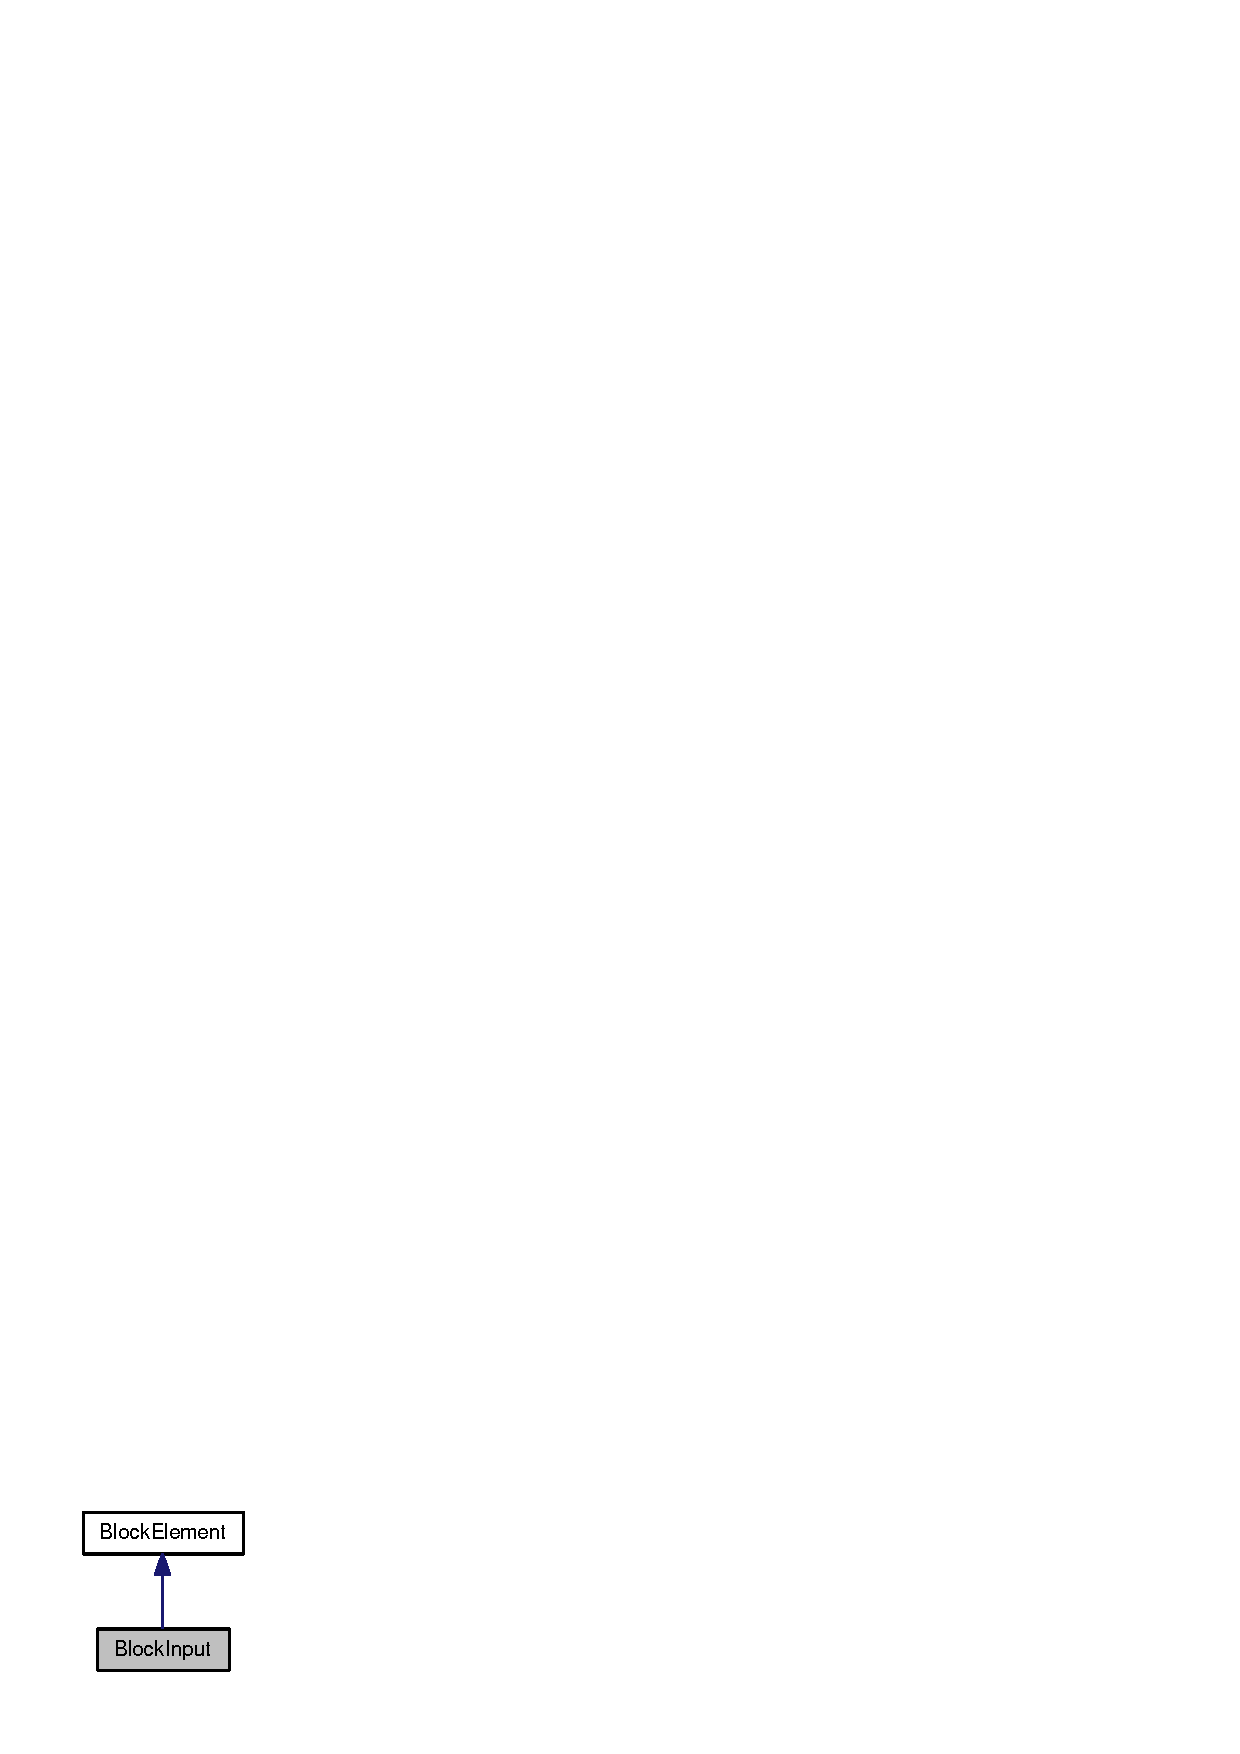
\includegraphics[width=60pt]{classBlockInput__inherit__graph}
\end{center}
\end{figure}
Collaboration diagram for BlockInput:\nopagebreak
\begin{figure}[H]
\begin{center}
\leavevmode
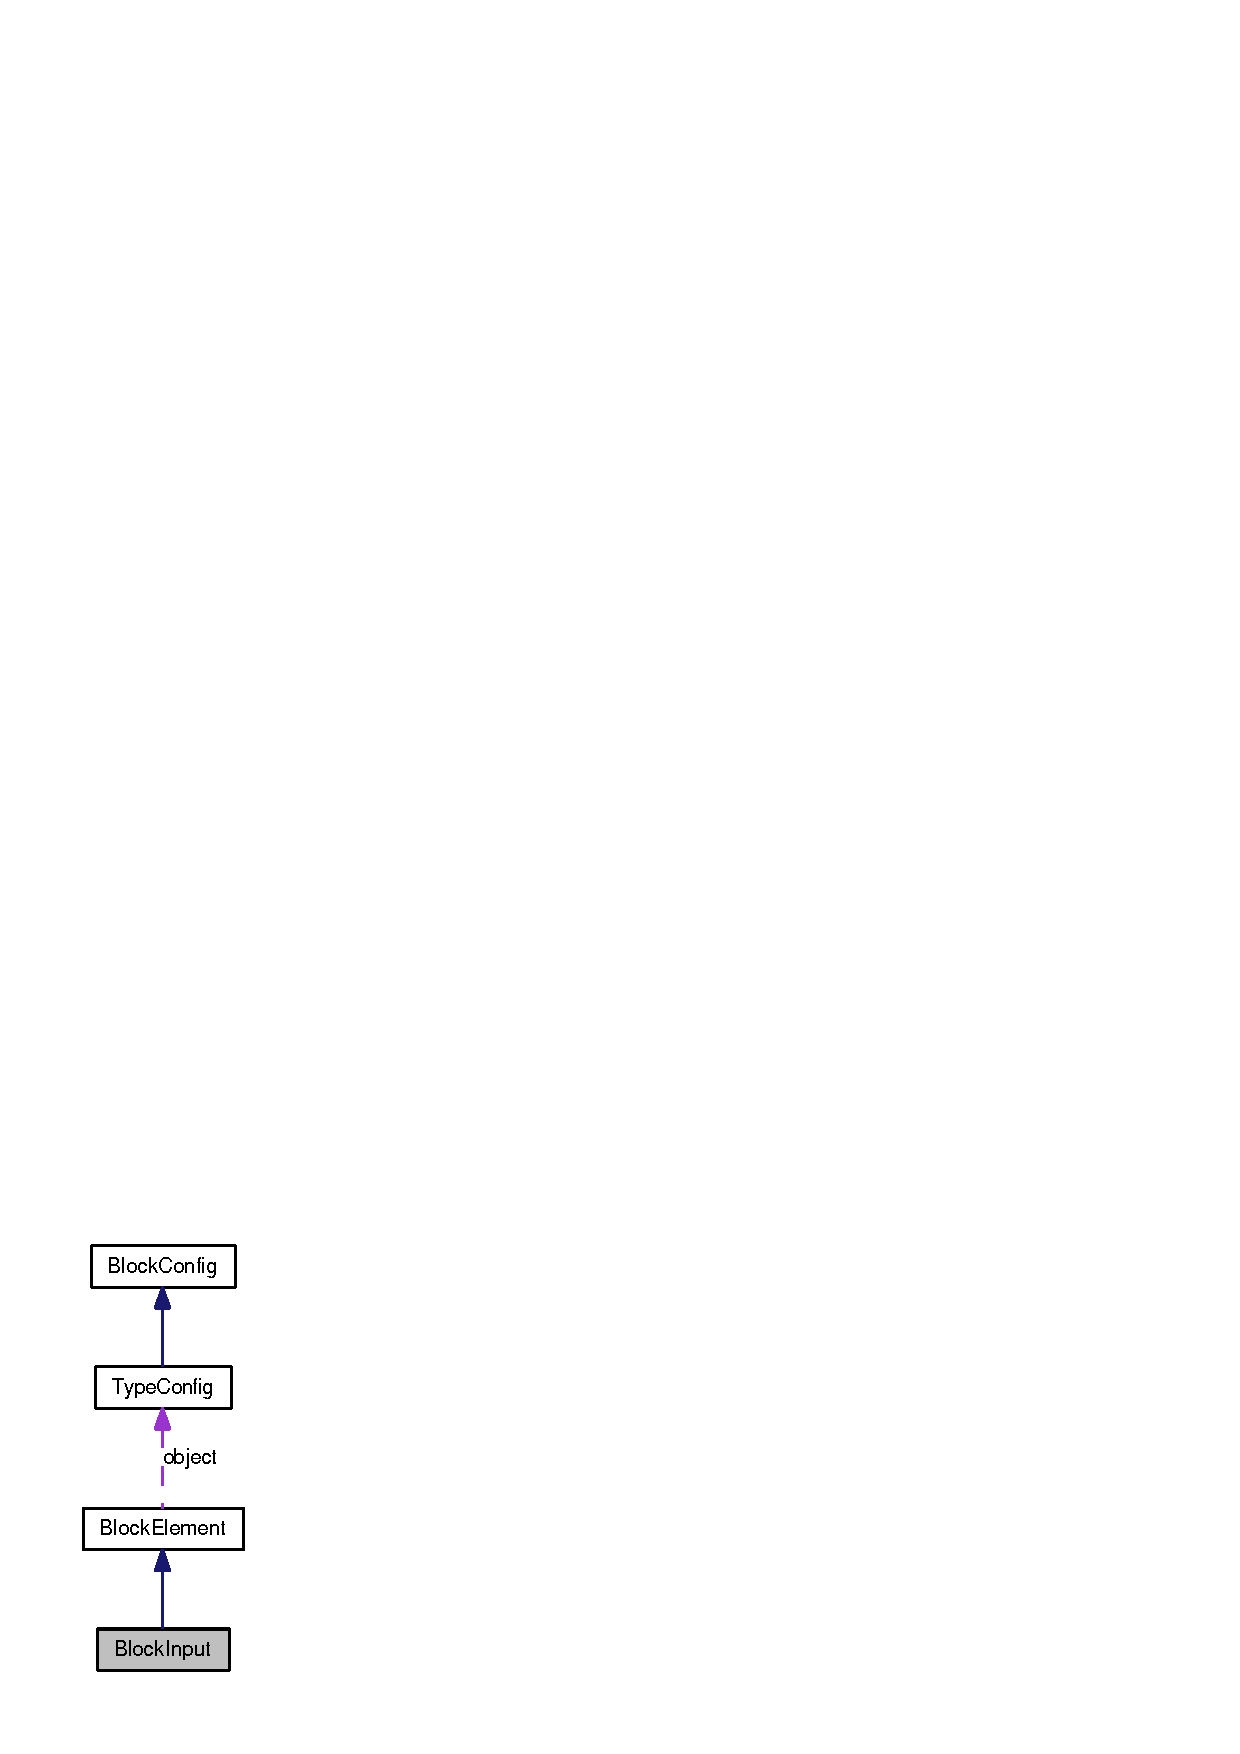
\includegraphics[width=60pt]{classBlockInput__coll__graph}
\end{center}
\end{figure}
\subsection*{Public Member Functions}
\begin{CompactItemize}
\item 
\hyperlink{classBlockInput_c5a561d29f79573620b13aa0b1df6138}{BlockInput} (const AnsiString aName)
\item 
\hyperlink{classBlockInput_07ca053b809a523114ab262bd049c59a}{BlockInput} (const \hyperlink{classBlockInput}{BlockInput} \&kopia)
\item 
\hyperlink{classBlockInput_b3ba18bff508ffeb192d2112accb7e43}{$\sim$BlockInput} ()
\item 
bool \hyperlink{classBlockInput_51f032cdaa57631902c512b716c8863c}{connect} (const AnsiString aName)
\item 
AnsiString \& \hyperlink{classBlockInput_a18ef5e360b351a058f75cc123532f55}{getConnectedType} ()
\item 
void \hyperlink{classBlockInput_438aec4b1b99763da696de529b199c67}{disconnect} ()
\end{CompactItemize}
\subsection*{Public Attributes}
\begin{CompactItemize}
\item 
vector$<$ AnsiString $>$ \hyperlink{classBlockInput_01da6f721998988559aa48370895e419}{allowedTypes}
\end{CompactItemize}
\subsection*{Private Attributes}
\begin{CompactItemize}
\item 
AnsiString \hyperlink{classBlockInput_dbbd1afff5c0211095d49ca4aa00191e}{inputType}
\end{CompactItemize}


\subsection{Detailed Description}
\hyperlink{classBlockInput}{BlockInput} - Klasa pojemnik przechowujaca wejscia i wyjscia bloku \begin{Desc}
\item[Author:]Piotr \end{Desc}
\begin{Desc}
\item[Date:]2008.11.25 \end{Desc}
\begin{Desc}
\item[Version:]0.1 \end{Desc}


Definition at line 15 of file BlockInput.h.

\subsection{Constructor \& Destructor Documentation}
\hypertarget{classBlockInput_c5a561d29f79573620b13aa0b1df6138}{
\index{BlockInput@{BlockInput}!BlockInput@{BlockInput}}
\index{BlockInput@{BlockInput}!BlockInput@{BlockInput}}
\subsubsection[BlockInput]{\setlength{\rightskip}{0pt plus 5cm}BlockInput::BlockInput (const AnsiString {\em aName})}}
\label{classBlockInput_c5a561d29f79573620b13aa0b1df6138}


Konstruktor \begin{Desc}
\item[Parameters:]
\begin{description}
\item[{\em aName}]nazwa wejscia bloku \end{description}
\end{Desc}


Definition at line 20 of file BlockInput.cpp.\hypertarget{classBlockInput_07ca053b809a523114ab262bd049c59a}{
\index{BlockInput@{BlockInput}!BlockInput@{BlockInput}}
\index{BlockInput@{BlockInput}!BlockInput@{BlockInput}}
\subsubsection[BlockInput]{\setlength{\rightskip}{0pt plus 5cm}BlockInput::BlockInput (const {\bf BlockInput} \& {\em kopia})}}
\label{classBlockInput_07ca053b809a523114ab262bd049c59a}


Konstruktor kopiujacy \begin{Desc}
\item[Parameters:]
\begin{description}
\item[{\em copy}]element ktory zostanie skopiowany \end{description}
\end{Desc}


Definition at line 24 of file BlockInput.cpp.

References allowedTypes, and inputType.\hypertarget{classBlockInput_b3ba18bff508ffeb192d2112accb7e43}{
\index{BlockInput@{BlockInput}!$\sim$BlockInput@{$\sim$BlockInput}}
\index{$\sim$BlockInput@{$\sim$BlockInput}!BlockInput@{BlockInput}}
\subsubsection[$\sim$BlockInput]{\setlength{\rightskip}{0pt plus 5cm}BlockInput::$\sim$BlockInput ()}}
\label{classBlockInput_b3ba18bff508ffeb192d2112accb7e43}


Destruktor 

Definition at line 30 of file BlockInput.cpp.

\subsection{Member Function Documentation}
\hypertarget{classBlockInput_51f032cdaa57631902c512b716c8863c}{
\index{BlockInput@{BlockInput}!connect@{connect}}
\index{connect@{connect}!BlockInput@{BlockInput}}
\subsubsection[connect]{\setlength{\rightskip}{0pt plus 5cm}bool BlockInput::connect (const AnsiString {\em aName})}}
\label{classBlockInput_51f032cdaa57631902c512b716c8863c}


Realizuje polaczenia mi�dzy blokami. \begin{Desc}
\item[Parameters:]
\begin{description}
\item[{\em aName}]nazwa obiektu z ktorym bedzie polaczone wejscie. \end{description}
\end{Desc}
\begin{Desc}
\item[Returns:]poprawnosc przeprowadzonej operajci. \end{Desc}


Definition at line 3 of file BlockInput.cpp.

References inputType.

Referenced by PIWOEngine::DuplcateSelectedBlocks(), PIWOEngine::loadFromFile(), and PIWOEngine::MakeConnection().\hypertarget{classBlockInput_a18ef5e360b351a058f75cc123532f55}{
\index{BlockInput@{BlockInput}!getConnectedType@{getConnectedType}}
\index{getConnectedType@{getConnectedType}!BlockInput@{BlockInput}}
\subsubsection[getConnectedType]{\setlength{\rightskip}{0pt plus 5cm}AnsiString \& BlockInput::getConnectedType ()}}
\label{classBlockInput_a18ef5e360b351a058f75cc123532f55}


Pobiera typ polaczenia. \begin{Desc}
\item[Returns:]nazwa typu polaczenia. \end{Desc}


Definition at line 15 of file BlockInput.cpp.

References inputType.

Referenced by VisualBlock::updateVisualComponents().\hypertarget{classBlockInput_438aec4b1b99763da696de529b199c67}{
\index{BlockInput@{BlockInput}!disconnect@{disconnect}}
\index{disconnect@{disconnect}!BlockInput@{BlockInput}}
\subsubsection[disconnect]{\setlength{\rightskip}{0pt plus 5cm}void BlockInput::disconnect ()}}
\label{classBlockInput_438aec4b1b99763da696de529b199c67}


rozlacza bloki 

Definition at line 10 of file BlockInput.cpp.

References inputType.

Referenced by PIWOEngine::DeleteSelectedConnection(), PIWOEngine::OnVisualBlockInputSelected(), and PIWOEngine::OnVisualBlockOutputSelected().

\subsection{Member Data Documentation}
\hypertarget{classBlockInput_dbbd1afff5c0211095d49ca4aa00191e}{
\index{BlockInput@{BlockInput}!inputType@{inputType}}
\index{inputType@{inputType}!BlockInput@{BlockInput}}
\subsubsection[inputType]{\setlength{\rightskip}{0pt plus 5cm}AnsiString {\bf BlockInput::inputType}\hspace{0.3cm}{\tt  \mbox{[}private\mbox{]}}}}
\label{classBlockInput_dbbd1afff5c0211095d49ca4aa00191e}




Definition at line 18 of file BlockInput.h.

Referenced by BlockInput(), connect(), disconnect(), and getConnectedType().\hypertarget{classBlockInput_01da6f721998988559aa48370895e419}{
\index{BlockInput@{BlockInput}!allowedTypes@{allowedTypes}}
\index{allowedTypes@{allowedTypes}!BlockInput@{BlockInput}}
\subsubsection[allowedTypes]{\setlength{\rightskip}{0pt plus 5cm}vector$<$AnsiString$>$ {\bf BlockInput::allowedTypes}}}
\label{classBlockInput_01da6f721998988559aa48370895e419}


lista dozwolonych typow kt�re moga zostac podane na wejscie 

Definition at line 37 of file BlockInput.h.

Referenced by BlockInput(), PIWOEngine::loadFromFile(), PIWOEngine::MakeConnection(), Connection::update(), and VisualBlock::updateVisualComponents().

The documentation for this class was generated from the following files:\begin{CompactItemize}
\item 
/PIWO/Program/engine/\hyperlink{BlockInput_8h}{BlockInput.h}\item 
/PIWO/Program/engine/\hyperlink{BlockInput_8cpp}{BlockInput.cpp}\end{CompactItemize}

\hypertarget{classBlockOutput}{
\section{BlockOutput Class Reference}
\label{classBlockOutput}\index{BlockOutput@{BlockOutput}}
}
{\tt \#include $<$BlockOutput.h$>$}

Inheritance diagram for BlockOutput:\nopagebreak
\begin{figure}[H]
\begin{center}
\leavevmode
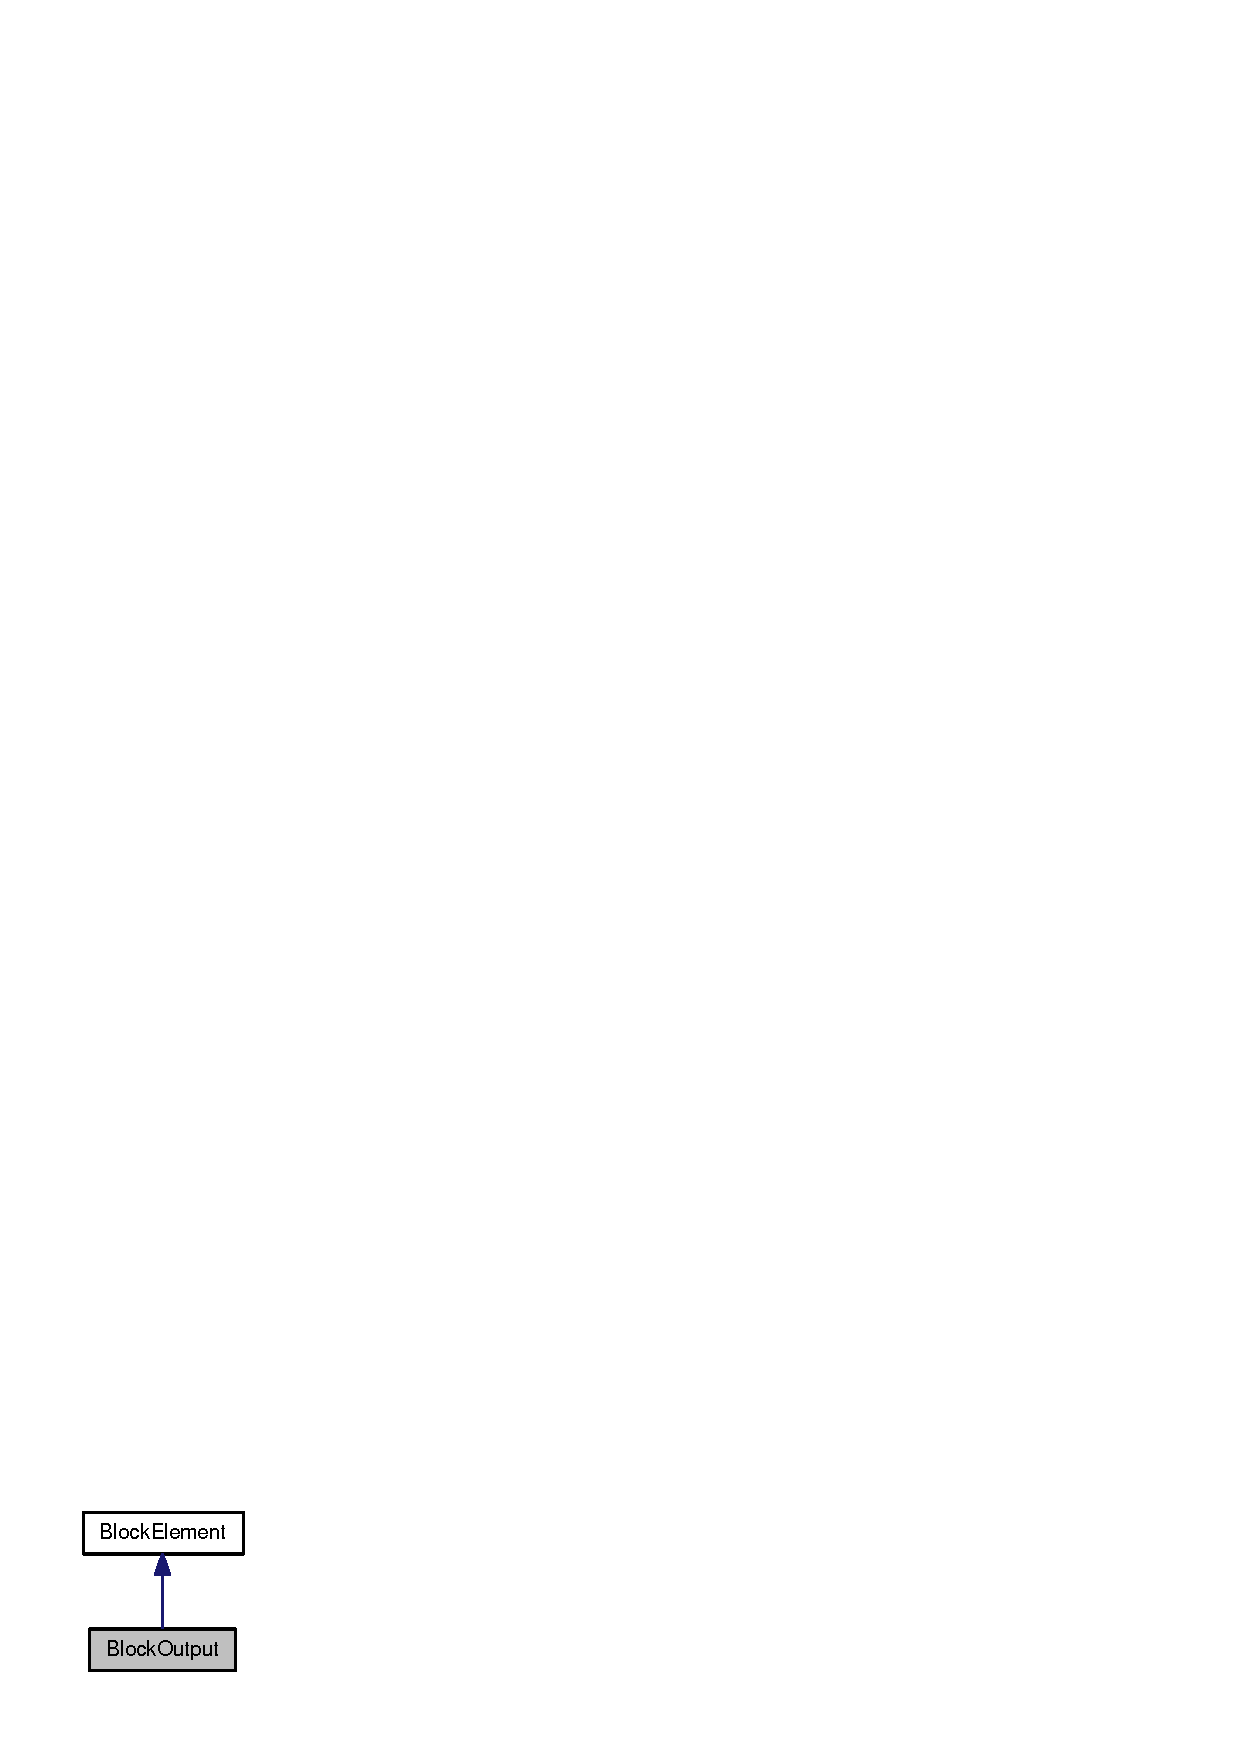
\includegraphics[width=60pt]{classBlockOutput__inherit__graph}
\end{center}
\end{figure}
Collaboration diagram for BlockOutput:\nopagebreak
\begin{figure}[H]
\begin{center}
\leavevmode
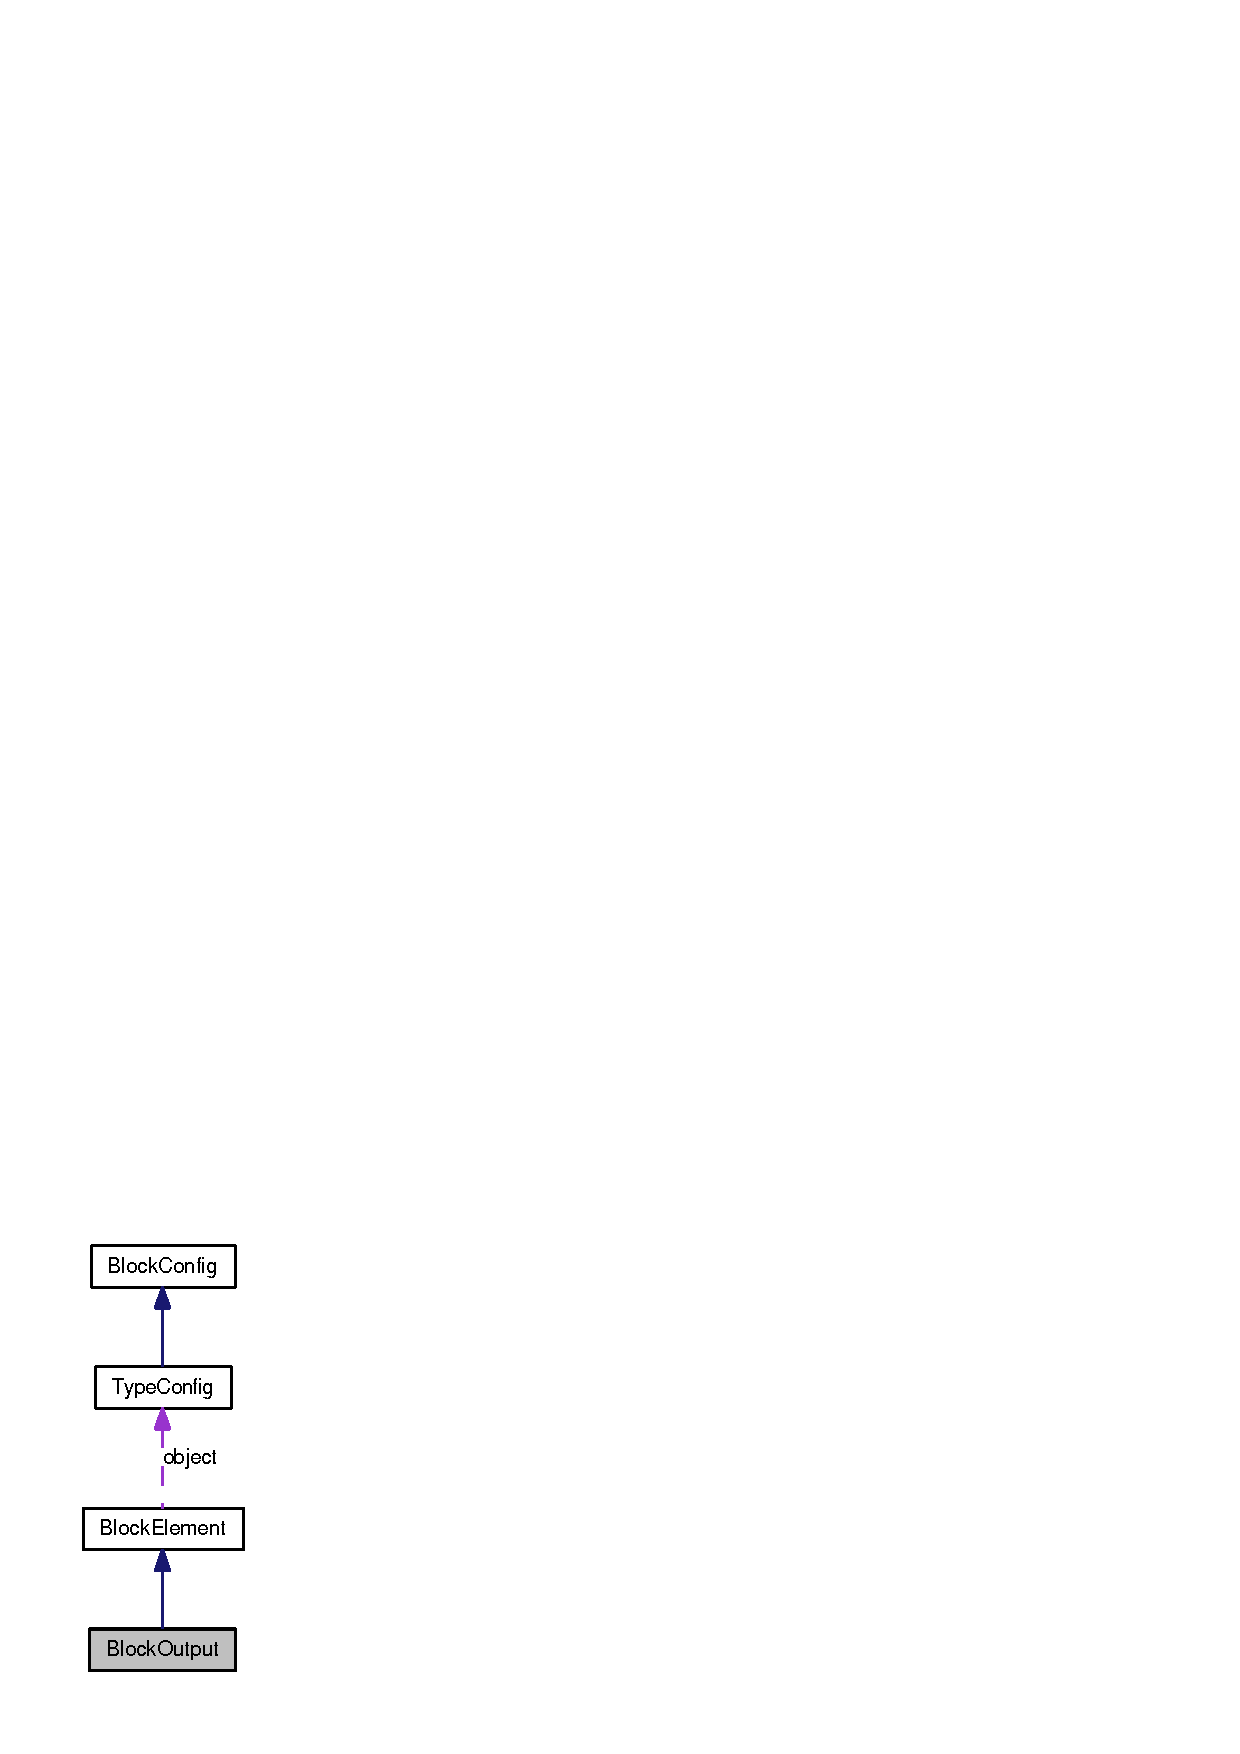
\includegraphics[width=60pt]{classBlockOutput__coll__graph}
\end{center}
\end{figure}
\subsection*{Public Member Functions}
\begin{CompactItemize}
\item 
\hyperlink{classBlockOutput_889e288fd7f8f4739b81681cd8975f63}{BlockOutput} (const AnsiString aName)
\item 
\hyperlink{classBlockOutput_d880f19249a89fd90bd08ec822aa6fd1}{BlockOutput} (const \hyperlink{classBlockOutput}{BlockOutput} \&copy)
\item 
\hyperlink{classBlockOutput_320d49ca840bb36f3f324730fc7af36a}{$\sim$BlockOutput} ()
\item 
AnsiString \& \hyperlink{classBlockOutput_da94ac502aea6bf1f1786e248a9d1d99}{getOutputType} ()
\item 
bool \hyperlink{classBlockOutput_9cc345b9f987e8d17bf8df7a334de8cd}{setOutputType} (AnsiString aName)
\end{CompactItemize}
\subsection*{Private Attributes}
\begin{CompactItemize}
\item 
AnsiString \hyperlink{classBlockOutput_80c32707c6e84083f5e69cf6170a3f26}{outputType}
\end{CompactItemize}


\subsection{Detailed Description}
\hyperlink{classBlockInput}{BlockInput} - Klasa pojemnik przechowujaca wejscia i wyjscia bloku \begin{Desc}
\item[Author:]Piotr \end{Desc}
\begin{Desc}
\item[Date:]2008.11.25 \end{Desc}
\begin{Desc}
\item[Version:]0.1 \end{Desc}


Definition at line 15 of file BlockOutput.h.

\subsection{Constructor \& Destructor Documentation}
\hypertarget{classBlockOutput_889e288fd7f8f4739b81681cd8975f63}{
\index{BlockOutput@{BlockOutput}!BlockOutput@{BlockOutput}}
\index{BlockOutput@{BlockOutput}!BlockOutput@{BlockOutput}}
\subsubsection[BlockOutput]{\setlength{\rightskip}{0pt plus 5cm}BlockOutput::BlockOutput (const AnsiString {\em aName})}}
\label{classBlockOutput_889e288fd7f8f4739b81681cd8975f63}


Konstruktor \begin{Desc}
\item[Parameters:]
\begin{description}
\item[{\em aName}]nazwa wyjscia. \end{description}
\end{Desc}


Definition at line 3 of file BlockOutput.cpp.\hypertarget{classBlockOutput_d880f19249a89fd90bd08ec822aa6fd1}{
\index{BlockOutput@{BlockOutput}!BlockOutput@{BlockOutput}}
\index{BlockOutput@{BlockOutput}!BlockOutput@{BlockOutput}}
\subsubsection[BlockOutput]{\setlength{\rightskip}{0pt plus 5cm}BlockOutput::BlockOutput (const {\bf BlockOutput} \& {\em copy})}}
\label{classBlockOutput_d880f19249a89fd90bd08ec822aa6fd1}


Konstruktor kopiujacy. \begin{Desc}
\item[Parameters:]
\begin{description}
\item[{\em copy}]obiekt ktory zostanie skopiowany \end{description}
\end{Desc}


Definition at line 7 of file BlockOutput.cpp.

References outputType.\hypertarget{classBlockOutput_320d49ca840bb36f3f324730fc7af36a}{
\index{BlockOutput@{BlockOutput}!$\sim$BlockOutput@{$\sim$BlockOutput}}
\index{$\sim$BlockOutput@{$\sim$BlockOutput}!BlockOutput@{BlockOutput}}
\subsubsection[$\sim$BlockOutput]{\setlength{\rightskip}{0pt plus 5cm}BlockOutput::$\sim$BlockOutput ()}}
\label{classBlockOutput_320d49ca840bb36f3f324730fc7af36a}


Destruktor 

Definition at line 12 of file BlockOutput.cpp.

\subsection{Member Function Documentation}
\hypertarget{classBlockOutput_da94ac502aea6bf1f1786e248a9d1d99}{
\index{BlockOutput@{BlockOutput}!getOutputType@{getOutputType}}
\index{getOutputType@{getOutputType}!BlockOutput@{BlockOutput}}
\subsubsection[getOutputType]{\setlength{\rightskip}{0pt plus 5cm}AnsiString \& BlockOutput::getOutputType ()}}
\label{classBlockOutput_da94ac502aea6bf1f1786e248a9d1d99}


Zwraca typ wyjscia. \begin{Desc}
\item[Returns:]AnsiString typ wyjscia \end{Desc}


Definition at line 16 of file BlockOutput.cpp.

References outputType.

Referenced by PIWOEngine::DuplcateSelectedBlocks(), PIWOEngine::loadFromFile(), PIWOEngine::MakeConnection(), Connection::update(), VisualBlock::updateVisualComponents(), and PIWOEngine::validateBlock().\hypertarget{classBlockOutput_9cc345b9f987e8d17bf8df7a334de8cd}{
\index{BlockOutput@{BlockOutput}!setOutputType@{setOutputType}}
\index{setOutputType@{setOutputType}!BlockOutput@{BlockOutput}}
\subsubsection[setOutputType]{\setlength{\rightskip}{0pt plus 5cm}bool BlockOutput::setOutputType (AnsiString {\em aName})}}
\label{classBlockOutput_9cc345b9f987e8d17bf8df7a334de8cd}


Ustawia typ wyjscia. \begin{Desc}
\item[Parameters:]
\begin{description}
\item[{\em aName}]typ wyjscia. \end{description}
\end{Desc}
\begin{Desc}
\item[Returns:]poprawnosc wykonanej operacji \end{Desc}


Definition at line 21 of file BlockOutput.cpp.

References outputType.

Referenced by PIWOEngine::loadFromFile().

\subsection{Member Data Documentation}
\hypertarget{classBlockOutput_80c32707c6e84083f5e69cf6170a3f26}{
\index{BlockOutput@{BlockOutput}!outputType@{outputType}}
\index{outputType@{outputType}!BlockOutput@{BlockOutput}}
\subsubsection[outputType]{\setlength{\rightskip}{0pt plus 5cm}AnsiString {\bf BlockOutput::outputType}\hspace{0.3cm}{\tt  \mbox{[}private\mbox{]}}}}
\label{classBlockOutput_80c32707c6e84083f5e69cf6170a3f26}




Definition at line 18 of file BlockOutput.h.

Referenced by BlockOutput(), getOutputType(), and setOutputType().

The documentation for this class was generated from the following files:\begin{CompactItemize}
\item 
/PIWO/Program/engine/\hyperlink{BlockOutput_8h}{BlockOutput.h}\item 
/PIWO/Program/engine/\hyperlink{BlockOutput_8cpp}{BlockOutput.cpp}\end{CompactItemize}

\hypertarget{classBlockValidateInputElement}{
\section{BlockValidateInputElement Class Reference}
\label{classBlockValidateInputElement}\index{BlockValidateInputElement@{BlockValidateInputElement}}
}
{\tt \#include $<$BlockValidateInputElement.h$>$}

Collaboration diagram for BlockValidateInputElement:\nopagebreak
\begin{figure}[H]
\begin{center}
\leavevmode
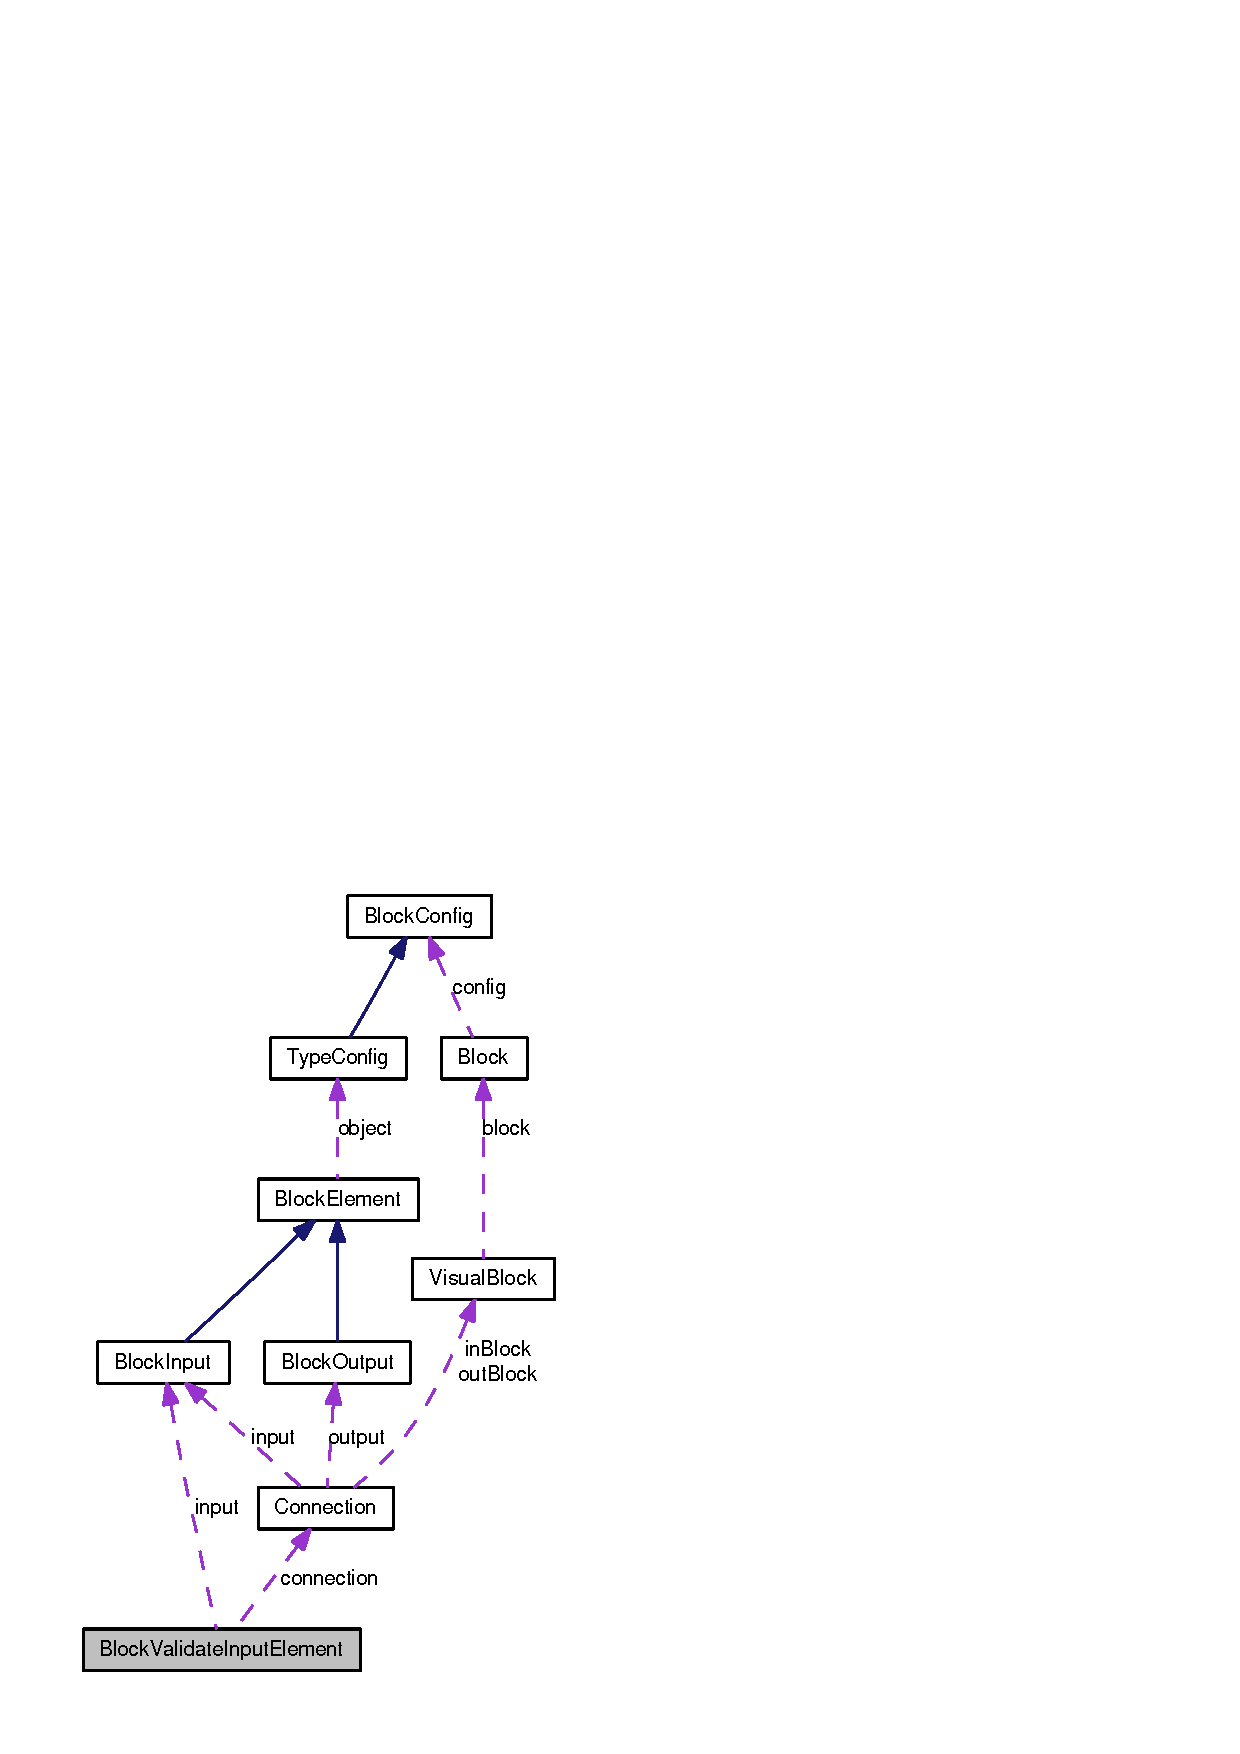
\includegraphics[height=400pt]{classBlockValidateInputElement__coll__graph}
\end{center}
\end{figure}
\subsection*{Public Attributes}
\begin{CompactItemize}
\item 
\hyperlink{classBlockInput}{BlockInput} $\ast$ \hyperlink{classBlockValidateInputElement_26eb9998699990af1bd5c37d0c349756}{input}
\item 
AnsiString \hyperlink{classBlockValidateInputElement_fde55132868604704517be802a6d49d6}{errorDescription}
\item 
int \hyperlink{classBlockValidateInputElement_4bfede90be866e8bfdda42c48ef54153}{errorCode}
\item 
\hyperlink{classConnection}{Connection} $\ast$ \hyperlink{classBlockValidateInputElement_fc5b397cb97ff9fe22948a97b3b782d1}{connection}
\end{CompactItemize}


\subsection{Detailed Description}
Klasa ta jest pojemnikiem, dla metody validateBlock w \hyperlink{classPIWOEngine}{PIWOEngine} 

Definition at line 10 of file BlockValidateInputElement.h.

\subsection{Member Data Documentation}
\hypertarget{classBlockValidateInputElement_26eb9998699990af1bd5c37d0c349756}{
\index{BlockValidateInputElement@{BlockValidateInputElement}!input@{input}}
\index{input@{input}!BlockValidateInputElement@{BlockValidateInputElement}}
\subsubsection[input]{\setlength{\rightskip}{0pt plus 5cm}{\bf BlockInput}$\ast$ {\bf BlockValidateInputElement::input}}}
\label{classBlockValidateInputElement_26eb9998699990af1bd5c37d0c349756}


Wskaznik do wejscia bloku 

Definition at line 16 of file BlockValidateInputElement.h.

Referenced by PIWOEngine::validateBlock().\hypertarget{classBlockValidateInputElement_fde55132868604704517be802a6d49d6}{
\index{BlockValidateInputElement@{BlockValidateInputElement}!errorDescription@{errorDescription}}
\index{errorDescription@{errorDescription}!BlockValidateInputElement@{BlockValidateInputElement}}
\subsubsection[errorDescription]{\setlength{\rightskip}{0pt plus 5cm}AnsiString {\bf BlockValidateInputElement::errorDescription}}}
\label{classBlockValidateInputElement_fde55132868604704517be802a6d49d6}


Komunikat bledu na tym wejsciu 

Definition at line 20 of file BlockValidateInputElement.h.

Referenced by PIWOEngine::validateBlock().\hypertarget{classBlockValidateInputElement_4bfede90be866e8bfdda42c48ef54153}{
\index{BlockValidateInputElement@{BlockValidateInputElement}!errorCode@{errorCode}}
\index{errorCode@{errorCode}!BlockValidateInputElement@{BlockValidateInputElement}}
\subsubsection[errorCode]{\setlength{\rightskip}{0pt plus 5cm}int {\bf BlockValidateInputElement::errorCode}}}
\label{classBlockValidateInputElement_4bfede90be866e8bfdda42c48ef54153}


Kod bledu na tym wejsciu 

Definition at line 24 of file BlockValidateInputElement.h.

Referenced by PIWOEngine::validateBlock().\hypertarget{classBlockValidateInputElement_fc5b397cb97ff9fe22948a97b3b782d1}{
\index{BlockValidateInputElement@{BlockValidateInputElement}!connection@{connection}}
\index{connection@{connection}!BlockValidateInputElement@{BlockValidateInputElement}}
\subsubsection[connection]{\setlength{\rightskip}{0pt plus 5cm}{\bf Connection}$\ast$ {\bf BlockValidateInputElement::connection}}}
\label{classBlockValidateInputElement_fc5b397cb97ff9fe22948a97b3b782d1}


Polaczenie aktualnie podlaczone do tego wejscia, lub NULL gdy go brak 

Definition at line 28 of file BlockValidateInputElement.h.

Referenced by PIWOEngine::validateBlock().

The documentation for this class was generated from the following file:\begin{CompactItemize}
\item 
/PIWO/Program/gui/\hyperlink{BlockValidateInputElement_8h}{BlockValidateInputElement.h}\end{CompactItemize}

\hypertarget{classBlockValidateOutputElement}{
\section{BlockValidateOutputElement Class Reference}
\label{classBlockValidateOutputElement}\index{BlockValidateOutputElement@{BlockValidateOutputElement}}
}
{\tt \#include $<$BlockValidateOutputElement.h$>$}

Collaboration diagram for BlockValidateOutputElement:\nopagebreak
\begin{figure}[H]
\begin{center}
\leavevmode
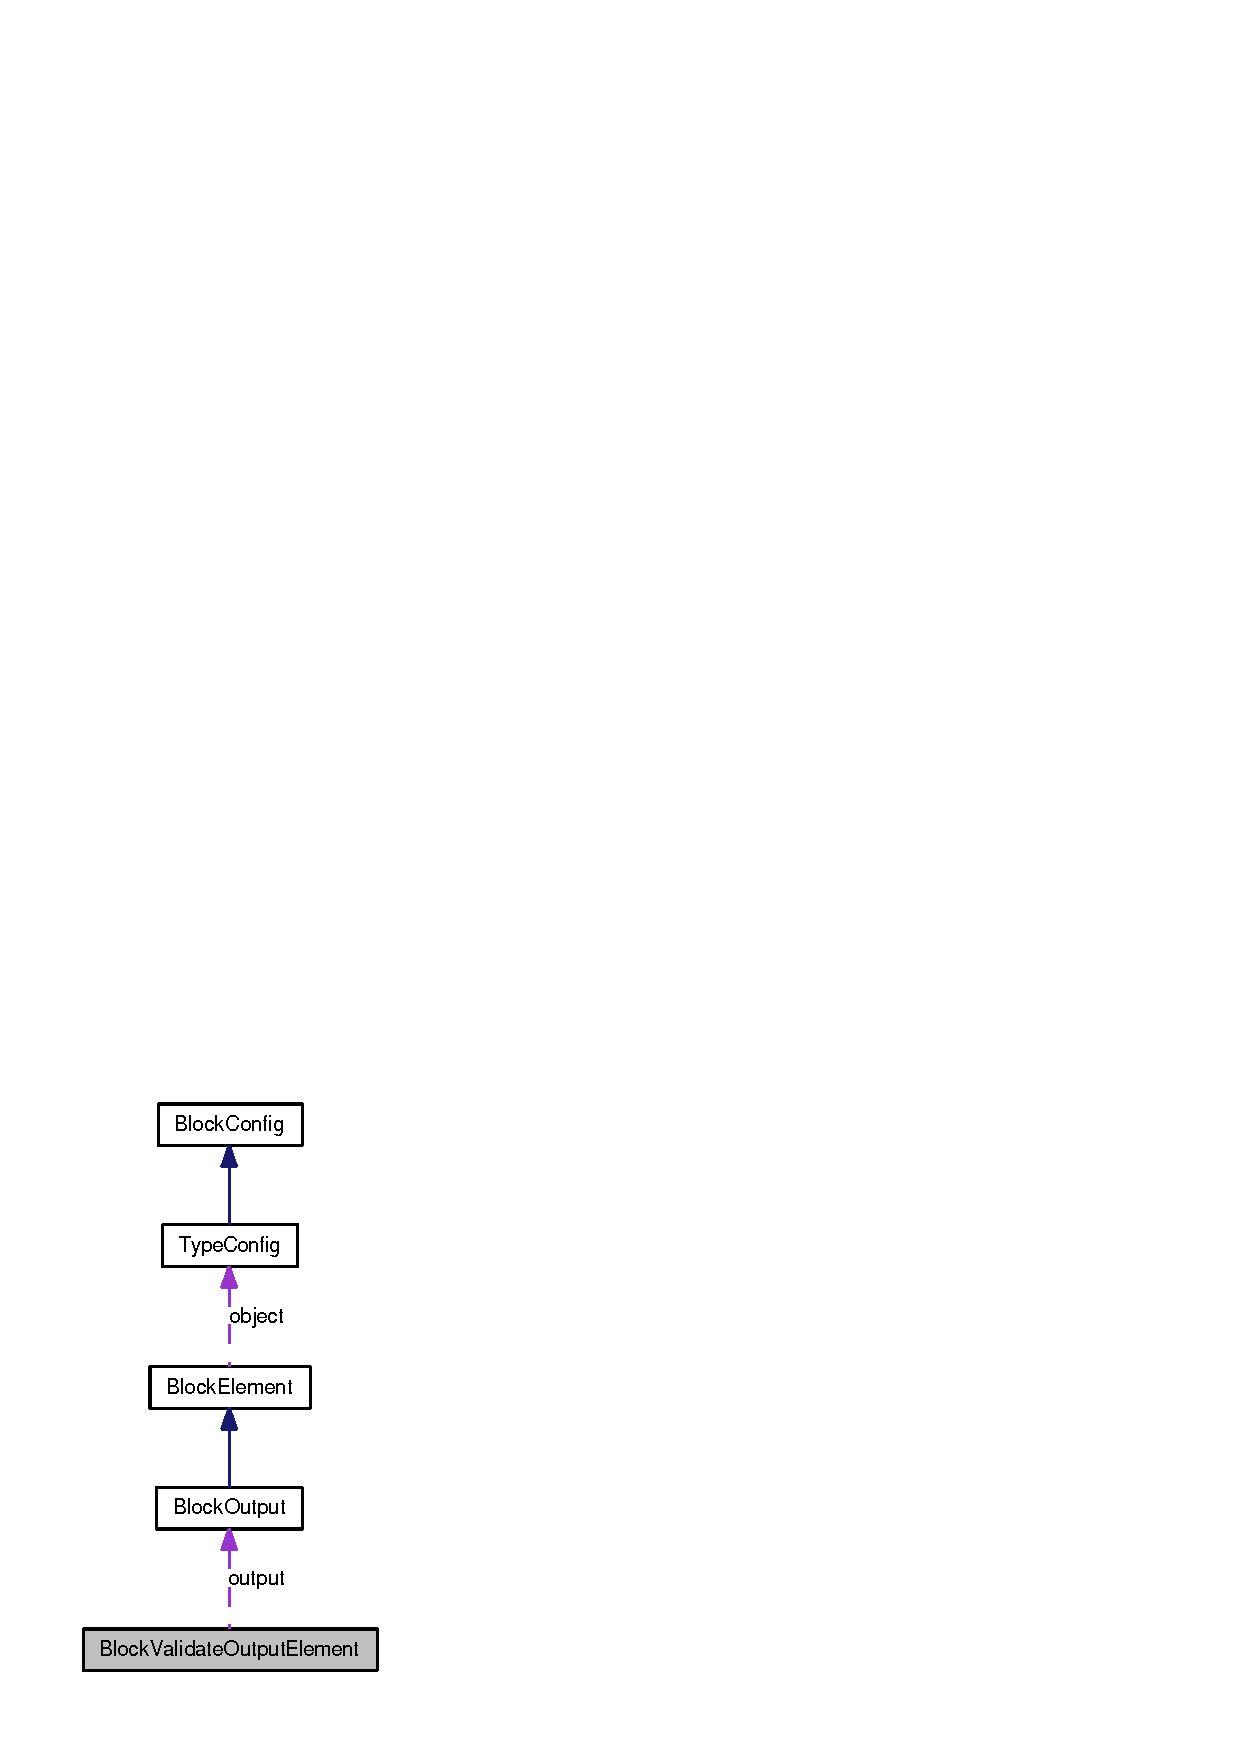
\includegraphics[width=92pt]{classBlockValidateOutputElement__coll__graph}
\end{center}
\end{figure}
\subsection*{Public Attributes}
\begin{CompactItemize}
\item 
\hyperlink{classBlockOutput}{BlockOutput} $\ast$ \hyperlink{classBlockValidateOutputElement_6dba2211ec248d6b57551f067689b7e6}{output}
\item 
AnsiString \hyperlink{classBlockValidateOutputElement_86efbb4dff759a82c0d7bf58889f7d54}{type}
\item 
AnsiString \hyperlink{classBlockValidateOutputElement_d063a4632a943e2972bba2dd77a77d02}{errorDescription}
\item 
int \hyperlink{classBlockValidateOutputElement_47eb7f8967002402ac8d4b1d6ec3abbf}{errorCode}
\item 
vector$<$ \hyperlink{classConnection}{Connection} $\ast$ $>$ \hyperlink{classBlockValidateOutputElement_7d6a09dcdc47578fe0580f342e45b78a}{connections}
\end{CompactItemize}


\subsection{Detailed Description}
Klasa ta jest pojemnikiem, dla metody validateBlock w \hyperlink{classPIWOEngine}{PIWOEngine} 

Definition at line 10 of file BlockValidateOutputElement.h.

\subsection{Member Data Documentation}
\hypertarget{classBlockValidateOutputElement_6dba2211ec248d6b57551f067689b7e6}{
\index{BlockValidateOutputElement@{BlockValidateOutputElement}!output@{output}}
\index{output@{output}!BlockValidateOutputElement@{BlockValidateOutputElement}}
\subsubsection[output]{\setlength{\rightskip}{0pt plus 5cm}{\bf BlockOutput}$\ast$ {\bf BlockValidateOutputElement::output}}}
\label{classBlockValidateOutputElement_6dba2211ec248d6b57551f067689b7e6}


Wskaznik do wyjscia tego bloku 

Definition at line 16 of file BlockValidateOutputElement.h.

Referenced by PIWOEngine::validateBlock().\hypertarget{classBlockValidateOutputElement_86efbb4dff759a82c0d7bf58889f7d54}{
\index{BlockValidateOutputElement@{BlockValidateOutputElement}!type@{type}}
\index{type@{type}!BlockValidateOutputElement@{BlockValidateOutputElement}}
\subsubsection[type]{\setlength{\rightskip}{0pt plus 5cm}AnsiString {\bf BlockValidateOutputElement::type}}}
\label{classBlockValidateOutputElement_86efbb4dff759a82c0d7bf58889f7d54}


Typ danych na tym wyjsciu 

Definition at line 20 of file BlockValidateOutputElement.h.

Referenced by PIWOEngine::validateBlock().\hypertarget{classBlockValidateOutputElement_d063a4632a943e2972bba2dd77a77d02}{
\index{BlockValidateOutputElement@{BlockValidateOutputElement}!errorDescription@{errorDescription}}
\index{errorDescription@{errorDescription}!BlockValidateOutputElement@{BlockValidateOutputElement}}
\subsubsection[errorDescription]{\setlength{\rightskip}{0pt plus 5cm}AnsiString {\bf BlockValidateOutputElement::errorDescription}}}
\label{classBlockValidateOutputElement_d063a4632a943e2972bba2dd77a77d02}


Opis bledu na tym wyjsciu 

Definition at line 24 of file BlockValidateOutputElement.h.

Referenced by PIWOEngine::validateBlock().\hypertarget{classBlockValidateOutputElement_47eb7f8967002402ac8d4b1d6ec3abbf}{
\index{BlockValidateOutputElement@{BlockValidateOutputElement}!errorCode@{errorCode}}
\index{errorCode@{errorCode}!BlockValidateOutputElement@{BlockValidateOutputElement}}
\subsubsection[errorCode]{\setlength{\rightskip}{0pt plus 5cm}int {\bf BlockValidateOutputElement::errorCode}}}
\label{classBlockValidateOutputElement_47eb7f8967002402ac8d4b1d6ec3abbf}


Kod bledu na tym wyjsciu 

Definition at line 28 of file BlockValidateOutputElement.h.

Referenced by PIWOEngine::validateBlock().\hypertarget{classBlockValidateOutputElement_7d6a09dcdc47578fe0580f342e45b78a}{
\index{BlockValidateOutputElement@{BlockValidateOutputElement}!connections@{connections}}
\index{connections@{connections}!BlockValidateOutputElement@{BlockValidateOutputElement}}
\subsubsection[connections]{\setlength{\rightskip}{0pt plus 5cm}vector$<${\bf Connection}$\ast$$>$ {\bf BlockValidateOutputElement::connections}}}
\label{classBlockValidateOutputElement_7d6a09dcdc47578fe0580f342e45b78a}


Wektor polaczen podlaczonych do tego wyjscia 

Definition at line 32 of file BlockValidateOutputElement.h.

Referenced by PIWOEngine::validateBlock().

The documentation for this class was generated from the following file:\begin{CompactItemize}
\item 
/PIWO/Program/gui/\hyperlink{BlockValidateOutputElement_8h}{BlockValidateOutputElement.h}\end{CompactItemize}

\hypertarget{classConnection}{
\section{Connection Class Reference}
\label{classConnection}\index{Connection@{Connection}}
}
{\tt \#include $<$Connection.h$>$}

Collaboration diagram for Connection:\nopagebreak
\begin{figure}[H]
\begin{center}
\leavevmode
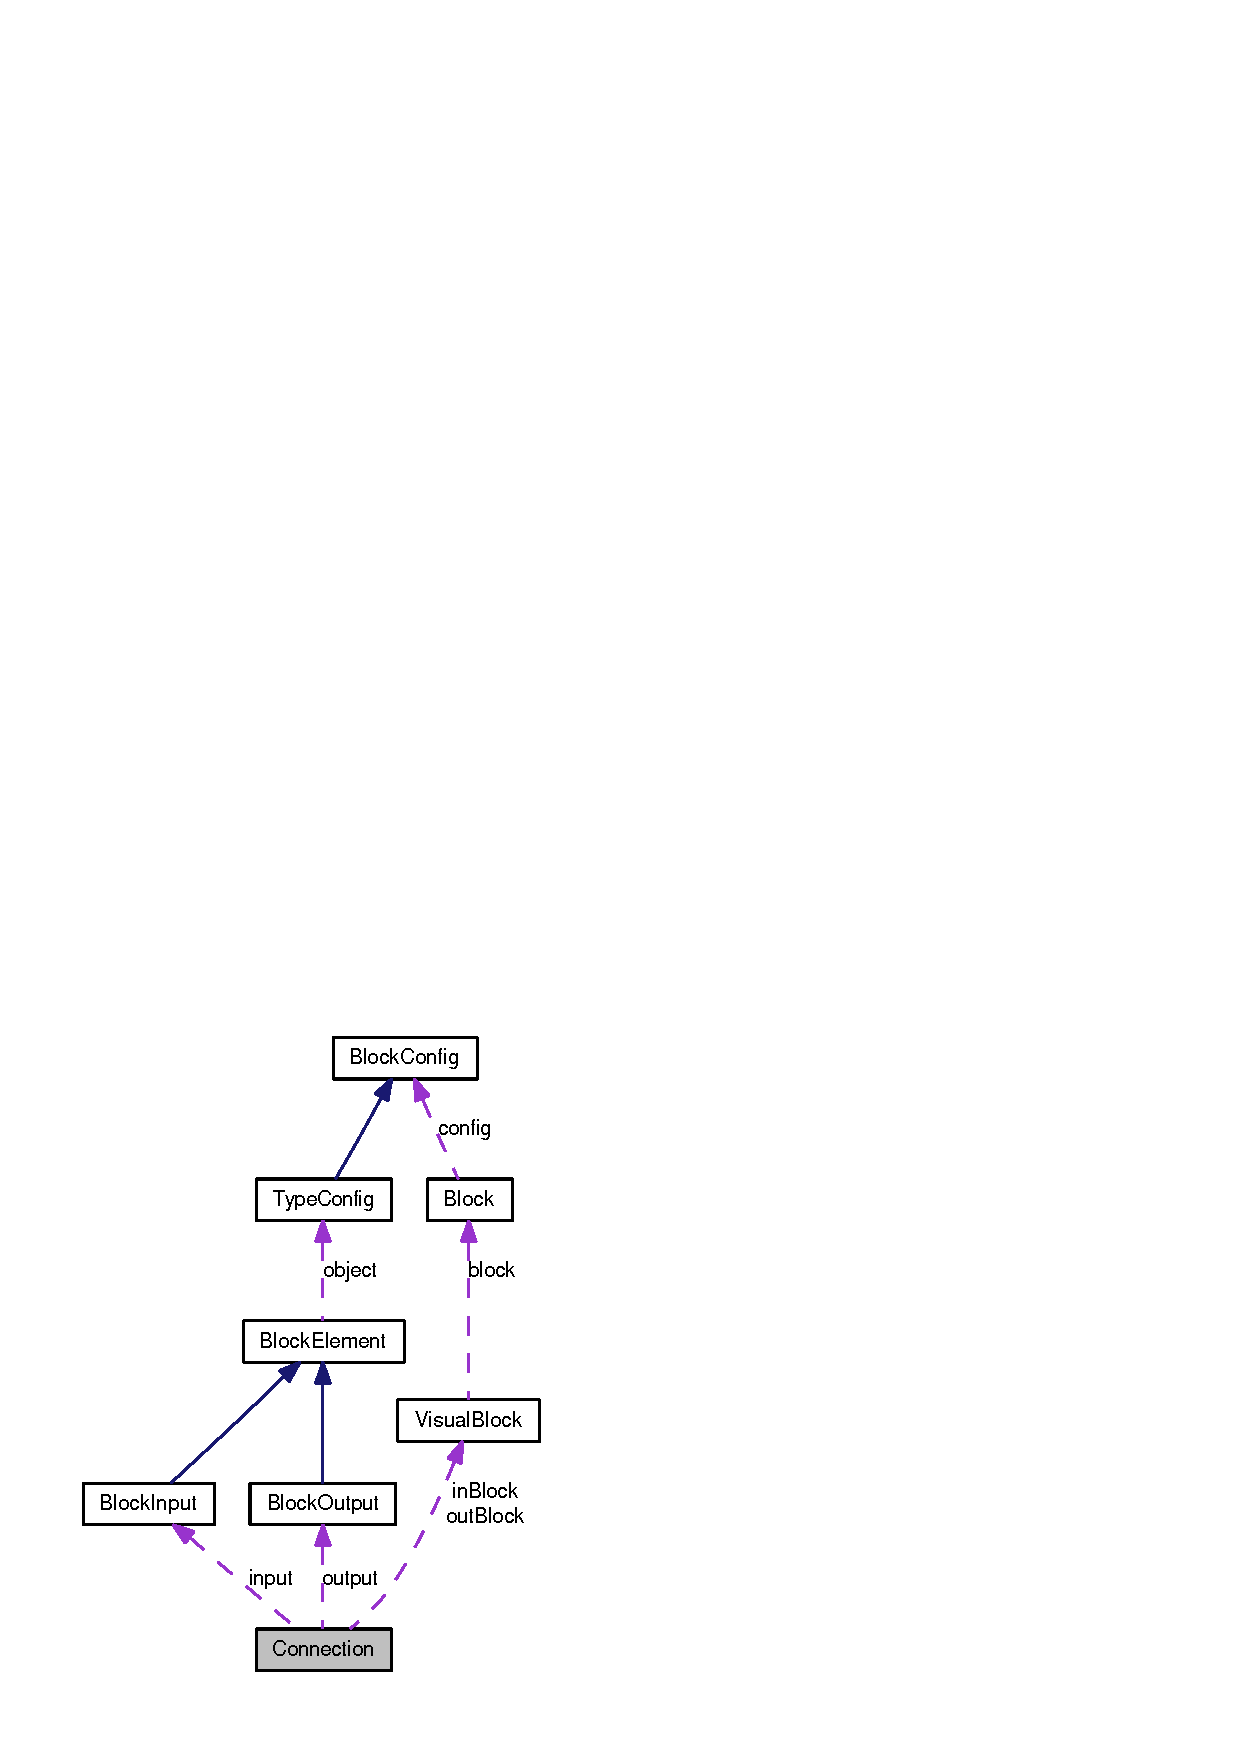
\includegraphics[width=131pt]{classConnection__coll__graph}
\end{center}
\end{figure}
\subsection*{Public Member Functions}
\begin{CompactItemize}
\item 
\hyperlink{classConnection_f539a9534b63a1b29fe5d8c3585bb9a1}{Connection} (TWinControl $\ast$owner)
\item 
\hyperlink{classConnection_2e4352edf667bea83001569e9da8a24d}{$\sim$Connection} ()
\item 
bool \hyperlink{classConnection_93953f74f832db3d351edc954a2caf1c}{draw} ()
\item 
bool \hyperlink{classConnection_2eae8606b02009ec2bbcd435541f702e}{update} ()
\item 
bool \hyperlink{classConnection_12c8e762f57cc902423543962e1dacd0}{connectionOk} ()
\item 
void \hyperlink{classConnection_cd027c03a7866907cf8a3c6fc3e9a104}{BringToFront} ()
\item 
void \hyperlink{classConnection_353faa06aa0d38ac5603cfca5744ac23}{setSelected} (bool s)
\item 
bool \hyperlink{classConnection_17fddf4c4d8c3d504d03f4914bdc2ebd}{getCustomizeState} ()
\item 
void \hyperlink{classConnection_c54097aa023bb0324ad932e3404b4cae}{setCustomizeFalse} ()
\end{CompactItemize}
\subsection*{Public Attributes}
\begin{CompactItemize}
\item 
\hyperlink{Connection_8h_e18f1161e76df22142d73ed0734bd10c}{Connection\_\-Function} \hyperlink{classConnection_d54a43c2dfb48de0b3737b1e02c0d422}{OnConnectionSelected}
\item 
\hyperlink{classBlockInput}{BlockInput} $\ast$ \hyperlink{classConnection_6c6649d08576878386a080c20131f6b9}{input}
\item 
\hyperlink{classBlockOutput}{BlockOutput} $\ast$ \hyperlink{classConnection_06a1d6005517d331a09c55a509f071cd}{output}
\item 
\hyperlink{classVisualBlock}{VisualBlock} $\ast$ \hyperlink{classConnection_75bfbbbce4d25e8c73560d560713c5a0}{inBlock}
\item 
\hyperlink{classVisualBlock}{VisualBlock} $\ast$ \hyperlink{classConnection_761e174ff27ed9e8935fb205453c6230}{outBlock}
\item 
AnsiString \hyperlink{classConnection_18e3620174b2a581799aa71c693f49d5}{typeOfConnection}
\item 
vector$<$ \hyperlink{classLine}{Line} $\ast$ $>$ \hyperlink{classConnection_fe8a072c88f8bc1b89a6c5986b7eca63}{lines}
\end{CompactItemize}
\subsection*{Private Member Functions}
\begin{CompactItemize}
\item 
void \hyperlink{classConnection_851fc1d97dad630deb54fa45693db7d0}{OnLineMove} (TObject $\ast$Sender)
\item 
void \hyperlink{classConnection_589c37b123edcf5fb159412366a5161b}{OnConnectionSelectedRequest} (TObject $\ast$Sender)
\item 
void \hyperlink{classConnection_469d5cb7dd9e48de17b532904522ecc2}{OnConnectionResetRequest} (TObject $\ast$Sender)
\item 
bool \hyperlink{classConnection_1f81b625a7de854874247655b05de071}{connectionOk} (\hyperlink{structPosition}{Position} \&in, \hyperlink{structPosition}{Position} \&out)
\item 
void \hyperlink{classConnection_d684c2b14e0b4f92537c39d0ec30b5f4}{redraw} (\hyperlink{structPosition}{Position} \&in, \hyperlink{structPosition}{Position} \&out)
\end{CompactItemize}
\subsection*{Private Attributes}
\begin{CompactItemize}
\item 
TWinControl $\ast$ \hyperlink{classConnection_2730afc4e0362071f2c8f1187899047b}{fowner}
\item 
int \hyperlink{classConnection_97d0ff34458fe4977e63e1a0e68b7278}{status}
\item 
bool \hyperlink{classConnection_24814ac50137c5bbd5ad387deeceaead}{selected}
\end{CompactItemize}


\subsection{Detailed Description}
\begin{Desc}
\item[Author:]Piotr Zegar \end{Desc}
\begin{Desc}
\item[Date:]2008.12.03 \end{Desc}
\begin{Desc}
\item[Version:]0.1\end{Desc}
Klasa zajmuje si� generowaniem po��cze� miedzy 2 blokami. 

Definition at line 35 of file Connection.h.

\subsection{Constructor \& Destructor Documentation}
\hypertarget{classConnection_f539a9534b63a1b29fe5d8c3585bb9a1}{
\index{Connection@{Connection}!Connection@{Connection}}
\index{Connection@{Connection}!Connection@{Connection}}
\subsubsection[Connection]{\setlength{\rightskip}{0pt plus 5cm}Connection::Connection (TWinControl $\ast$ {\em owner})}}
\label{classConnection_f539a9534b63a1b29fe5d8c3585bb9a1}




Definition at line 6 of file Connection.cpp.

References fowner, inBlock, input, OnConnectionSelected, outBlock, output, selected, and status.\hypertarget{classConnection_2e4352edf667bea83001569e9da8a24d}{
\index{Connection@{Connection}!$\sim$Connection@{$\sim$Connection}}
\index{$\sim$Connection@{$\sim$Connection}!Connection@{Connection}}
\subsubsection[$\sim$Connection]{\setlength{\rightskip}{0pt plus 5cm}Connection::$\sim$Connection ()}}
\label{classConnection_2e4352edf667bea83001569e9da8a24d}




Definition at line 18 of file Connection.cpp.

References lines.

\subsection{Member Function Documentation}
\hypertarget{classConnection_851fc1d97dad630deb54fa45693db7d0}{
\index{Connection@{Connection}!OnLineMove@{OnLineMove}}
\index{OnLineMove@{OnLineMove}!Connection@{Connection}}
\subsubsection[OnLineMove]{\setlength{\rightskip}{0pt plus 5cm}void Connection::OnLineMove (TObject $\ast$ {\em Sender})\hspace{0.3cm}{\tt  \mbox{[}private\mbox{]}}}}
\label{classConnection_851fc1d97dad630deb54fa45693db7d0}




Definition at line 292 of file Connection.cpp.

References draw().

Referenced by draw().\hypertarget{classConnection_589c37b123edcf5fb159412366a5161b}{
\index{Connection@{Connection}!OnConnectionSelectedRequest@{OnConnectionSelectedRequest}}
\index{OnConnectionSelectedRequest@{OnConnectionSelectedRequest}!Connection@{Connection}}
\subsubsection[OnConnectionSelectedRequest]{\setlength{\rightskip}{0pt plus 5cm}void Connection::OnConnectionSelectedRequest (TObject $\ast$ {\em Sender})\hspace{0.3cm}{\tt  \mbox{[}private\mbox{]}}}}
\label{classConnection_589c37b123edcf5fb159412366a5161b}




Definition at line 297 of file Connection.cpp.

References BringToFront(), OnConnectionSelected, selected, and setSelected().

Referenced by draw().\hypertarget{classConnection_469d5cb7dd9e48de17b532904522ecc2}{
\index{Connection@{Connection}!OnConnectionResetRequest@{OnConnectionResetRequest}}
\index{OnConnectionResetRequest@{OnConnectionResetRequest}!Connection@{Connection}}
\subsubsection[OnConnectionResetRequest]{\setlength{\rightskip}{0pt plus 5cm}void Connection::OnConnectionResetRequest (TObject $\ast$ {\em Sender})\hspace{0.3cm}{\tt  \mbox{[}private\mbox{]}}}}
\label{classConnection_469d5cb7dd9e48de17b532904522ecc2}




Definition at line 307 of file Connection.cpp.

References draw(), and lines.

Referenced by draw().\hypertarget{classConnection_1f81b625a7de854874247655b05de071}{
\index{Connection@{Connection}!connectionOk@{connectionOk}}
\index{connectionOk@{connectionOk}!Connection@{Connection}}
\subsubsection[connectionOk]{\setlength{\rightskip}{0pt plus 5cm}bool Connection::connectionOk ({\bf Position} \& {\em in}, \/  {\bf Position} \& {\em out})\hspace{0.3cm}{\tt  \mbox{[}private\mbox{]}}}}
\label{classConnection_1f81b625a7de854874247655b05de071}




Definition at line 27 of file Connection.cpp.

References Position::direction, lines, and Position::xy.\hypertarget{classConnection_d684c2b14e0b4f92537c39d0ec30b5f4}{
\index{Connection@{Connection}!redraw@{redraw}}
\index{redraw@{redraw}!Connection@{Connection}}
\subsubsection[redraw]{\setlength{\rightskip}{0pt plus 5cm}void Connection::redraw ({\bf Position} \& {\em in}, \/  {\bf Position} \& {\em out})\hspace{0.3cm}{\tt  \mbox{[}private\mbox{]}}}}
\label{classConnection_d684c2b14e0b4f92537c39d0ec30b5f4}




Definition at line 79 of file Connection.cpp.

References Position::direction, inBlock, lines, outBlock, and Position::xy.

Referenced by draw().\hypertarget{classConnection_93953f74f832db3d351edc954a2caf1c}{
\index{Connection@{Connection}!draw@{draw}}
\index{draw@{draw}!Connection@{Connection}}
\subsubsection[draw]{\setlength{\rightskip}{0pt plus 5cm}bool Connection::draw ()}}
\label{classConnection_93953f74f832db3d351edc954a2caf1c}




Definition at line 147 of file Connection.cpp.

References connectionOk(), Position::direction, fowner, VisualBlock::getInputPosition(), VisualBlock::getOutputPosition(), inBlock, input, lines, OnConnectionResetRequest(), Line::OnConnectionResetRequest, OnConnectionSelectedRequest(), Line::OnConnectionSelectRequest, OnLineMove(), Line::OnLineMove, outBlock, output, and redraw().

Referenced by PIWOEngine::DuplcateSelectedBlocks(), PIWOEngine::loadFromFile(), PIWOEngine::MakeConnection(), OnConnectionResetRequest(), OnLineMove(), and setCustomizeFalse().\hypertarget{classConnection_2eae8606b02009ec2bbcd435541f702e}{
\index{Connection@{Connection}!update@{update}}
\index{update@{update}!Connection@{Connection}}
\subsubsection[update]{\setlength{\rightskip}{0pt plus 5cm}bool Connection::update ()}}
\label{classConnection_2eae8606b02009ec2bbcd435541f702e}




Definition at line 191 of file Connection.cpp.

References BlockInput::allowedTypes, ConnectionErrorNormalColor, ConnectionErrorSelectedColor, ConnectionOkNormalColor, ConnectionOkSelectedColor, ConnectionWarrningNormalColor, ConnectionWarrningSelectedColor, BlockElement::getDescription(), BlockElement::getErrorCode(), BlockElement::getErrorDescription(), BlockOutput::getOutputType(), VisualBlock::getTitle(), inBlock, input, lines, outBlock, output, selected, status, and typeOfConnection.

Referenced by PIWOEngine::DuplcateSelectedBlocks(), PIWOEngine::loadFromFile(), PIWOEngine::MakeConnection(), and PIWOEngine::runBlock().\hypertarget{classConnection_12c8e762f57cc902423543962e1dacd0}{
\index{Connection@{Connection}!connectionOk@{connectionOk}}
\index{connectionOk@{connectionOk}!Connection@{Connection}}
\subsubsection[connectionOk]{\setlength{\rightskip}{0pt plus 5cm}bool Connection::connectionOk ()}}
\label{classConnection_12c8e762f57cc902423543962e1dacd0}




Definition at line 70 of file Connection.cpp.

References VisualBlock::getInputPosition(), VisualBlock::getOutputPosition(), inBlock, input, lines, outBlock, and output.

Referenced by draw().\hypertarget{classConnection_cd027c03a7866907cf8a3c6fc3e9a104}{
\index{Connection@{Connection}!BringToFront@{BringToFront}}
\index{BringToFront@{BringToFront}!Connection@{Connection}}
\subsubsection[BringToFront]{\setlength{\rightskip}{0pt plus 5cm}void Connection::BringToFront ()}}
\label{classConnection_cd027c03a7866907cf8a3c6fc3e9a104}




Definition at line 258 of file Connection.cpp.

References lines.

Referenced by PIWOEngine::OnConnectionSelect(), and OnConnectionSelectedRequest().\hypertarget{classConnection_353faa06aa0d38ac5603cfca5744ac23}{
\index{Connection@{Connection}!setSelected@{setSelected}}
\index{setSelected@{setSelected}!Connection@{Connection}}
\subsubsection[setSelected]{\setlength{\rightskip}{0pt plus 5cm}void Connection::setSelected (bool {\em s})}}
\label{classConnection_353faa06aa0d38ac5603cfca5744ac23}




Definition at line 266 of file Connection.cpp.

References ConnectionErrorNormalColor, ConnectionErrorSelectedColor, ConnectionOkNormalColor, ConnectionOkSelectedColor, ConnectionWarrningNormalColor, ConnectionWarrningSelectedColor, lines, selected, and status.

Referenced by PIWOEngine::MakeConnection(), PIWOEngine::OnConnectionSelect(), OnConnectionSelectedRequest(), and PIWOEngine::UnselectSelectedConnection().\hypertarget{classConnection_17fddf4c4d8c3d504d03f4914bdc2ebd}{
\index{Connection@{Connection}!getCustomizeState@{getCustomizeState}}
\index{getCustomizeState@{getCustomizeState}!Connection@{Connection}}
\subsubsection[getCustomizeState]{\setlength{\rightskip}{0pt plus 5cm}bool Connection::getCustomizeState ()}}
\label{classConnection_17fddf4c4d8c3d504d03f4914bdc2ebd}




Definition at line 317 of file Connection.cpp.

References lines.\hypertarget{classConnection_c54097aa023bb0324ad932e3404b4cae}{
\index{Connection@{Connection}!setCustomizeFalse@{setCustomizeFalse}}
\index{setCustomizeFalse@{setCustomizeFalse}!Connection@{Connection}}
\subsubsection[setCustomizeFalse]{\setlength{\rightskip}{0pt plus 5cm}void Connection::setCustomizeFalse ()}}
\label{classConnection_c54097aa023bb0324ad932e3404b4cae}




Definition at line 326 of file Connection.cpp.

References draw(), and lines.

Referenced by PIWOEngine::CancelCustomizationOnSelectedConnections().

\subsection{Member Data Documentation}
\hypertarget{classConnection_2730afc4e0362071f2c8f1187899047b}{
\index{Connection@{Connection}!fowner@{fowner}}
\index{fowner@{fowner}!Connection@{Connection}}
\subsubsection[fowner]{\setlength{\rightskip}{0pt plus 5cm}TWinControl$\ast$ {\bf Connection::fowner}\hspace{0.3cm}{\tt  \mbox{[}private\mbox{]}}}}
\label{classConnection_2730afc4e0362071f2c8f1187899047b}




Definition at line 38 of file Connection.h.

Referenced by Connection(), and draw().\hypertarget{classConnection_97d0ff34458fe4977e63e1a0e68b7278}{
\index{Connection@{Connection}!status@{status}}
\index{status@{status}!Connection@{Connection}}
\subsubsection[status]{\setlength{\rightskip}{0pt plus 5cm}int {\bf Connection::status}\hspace{0.3cm}{\tt  \mbox{[}private\mbox{]}}}}
\label{classConnection_97d0ff34458fe4977e63e1a0e68b7278}




Definition at line 39 of file Connection.h.

Referenced by Connection(), setSelected(), and update().\hypertarget{classConnection_24814ac50137c5bbd5ad387deeceaead}{
\index{Connection@{Connection}!selected@{selected}}
\index{selected@{selected}!Connection@{Connection}}
\subsubsection[selected]{\setlength{\rightskip}{0pt plus 5cm}bool {\bf Connection::selected}\hspace{0.3cm}{\tt  \mbox{[}private\mbox{]}}}}
\label{classConnection_24814ac50137c5bbd5ad387deeceaead}




Definition at line 40 of file Connection.h.

Referenced by Connection(), OnConnectionSelectedRequest(), setSelected(), and update().\hypertarget{classConnection_d54a43c2dfb48de0b3737b1e02c0d422}{
\index{Connection@{Connection}!OnConnectionSelected@{OnConnectionSelected}}
\index{OnConnectionSelected@{OnConnectionSelected}!Connection@{Connection}}
\subsubsection[OnConnectionSelected]{\setlength{\rightskip}{0pt plus 5cm}{\bf Connection\_\-Function} {\bf Connection::OnConnectionSelected}}}
\label{classConnection_d54a43c2dfb48de0b3737b1e02c0d422}




Definition at line 49 of file Connection.h.

Referenced by Connection(), PIWOEngine::DuplcateSelectedBlocks(), PIWOEngine::loadFromFile(), PIWOEngine::MakeConnection(), and OnConnectionSelectedRequest().\hypertarget{classConnection_6c6649d08576878386a080c20131f6b9}{
\index{Connection@{Connection}!input@{input}}
\index{input@{input}!Connection@{Connection}}
\subsubsection[input]{\setlength{\rightskip}{0pt plus 5cm}{\bf BlockInput}$\ast$ {\bf Connection::input}}}
\label{classConnection_6c6649d08576878386a080c20131f6b9}




Definition at line 51 of file Connection.h.

Referenced by PIWOEngine::CancelCustomizationOnSelectedConnections(), Connection(), connectionOk(), PIWOEngine::DeleteSelectedConnection(), draw(), PIWOEngine::DuplcateSelectedBlocks(), PIWOEngine::loadFromFile(), PIWOEngine::MakeConnection(), PIWOEngine::OnConnectionSelect(), PIWOEngine::OnVisualBlockInputSelected(), PIWOEngine::OnVisualBlockOutputSelected(), PIWOEngine::UnselectSelectedConnection(), and update().\hypertarget{classConnection_06a1d6005517d331a09c55a509f071cd}{
\index{Connection@{Connection}!output@{output}}
\index{output@{output}!Connection@{Connection}}
\subsubsection[output]{\setlength{\rightskip}{0pt plus 5cm}{\bf BlockOutput}$\ast$ {\bf Connection::output}}}
\label{classConnection_06a1d6005517d331a09c55a509f071cd}




Definition at line 52 of file Connection.h.

Referenced by PIWOEngine::CancelCustomizationOnSelectedConnections(), Connection(), connectionOk(), PIWOEngine::DeleteSelectedConnection(), draw(), PIWOEngine::DuplcateSelectedBlocks(), PIWOEngine::loadFromFile(), PIWOEngine::MakeConnection(), PIWOEngine::OnConnectionSelect(), PIWOEngine::OnVisualBlockInputSelected(), PIWOEngine::OnVisualBlockOutputSelected(), PIWOEngine::runBlock(), PIWOEngine::UnselectSelectedConnection(), and update().\hypertarget{classConnection_75bfbbbce4d25e8c73560d560713c5a0}{
\index{Connection@{Connection}!inBlock@{inBlock}}
\index{inBlock@{inBlock}!Connection@{Connection}}
\subsubsection[inBlock]{\setlength{\rightskip}{0pt plus 5cm}{\bf VisualBlock}$\ast$ {\bf Connection::inBlock}}}
\label{classConnection_75bfbbbce4d25e8c73560d560713c5a0}




Definition at line 53 of file Connection.h.

Referenced by PIWOEngine::CancelCustomizationOnSelectedConnections(), Connection(), connectionOk(), PIWOEngine::DeleteSelectedConnection(), draw(), PIWOEngine::DuplcateSelectedBlocks(), PIWOEngine::loadFromFile(), PIWOEngine::MakeConnection(), PIWOEngine::OnConnectionSelect(), PIWOEngine::OnVisualBlockInputSelected(), PIWOEngine::OnVisualBlockOutputSelected(), redraw(), PIWOEngine::UnselectSelectedConnection(), and update().\hypertarget{classConnection_761e174ff27ed9e8935fb205453c6230}{
\index{Connection@{Connection}!outBlock@{outBlock}}
\index{outBlock@{outBlock}!Connection@{Connection}}
\subsubsection[outBlock]{\setlength{\rightskip}{0pt plus 5cm}{\bf VisualBlock}$\ast$ {\bf Connection::outBlock}}}
\label{classConnection_761e174ff27ed9e8935fb205453c6230}




Definition at line 54 of file Connection.h.

Referenced by PIWOEngine::CancelCustomizationOnSelectedConnections(), Connection(), connectionOk(), PIWOEngine::DeleteSelectedConnection(), draw(), PIWOEngine::DuplcateSelectedBlocks(), PIWOEngine::loadFromFile(), PIWOEngine::MakeConnection(), PIWOEngine::OnConnectionSelect(), PIWOEngine::OnVisualBlockInputSelected(), PIWOEngine::OnVisualBlockOutputSelected(), redraw(), PIWOEngine::runBlock(), PIWOEngine::UnselectSelectedConnection(), and update().\hypertarget{classConnection_18e3620174b2a581799aa71c693f49d5}{
\index{Connection@{Connection}!typeOfConnection@{typeOfConnection}}
\index{typeOfConnection@{typeOfConnection}!Connection@{Connection}}
\subsubsection[typeOfConnection]{\setlength{\rightskip}{0pt plus 5cm}AnsiString {\bf Connection::typeOfConnection}}}
\label{classConnection_18e3620174b2a581799aa71c693f49d5}




Definition at line 55 of file Connection.h.

Referenced by update().\hypertarget{classConnection_fe8a072c88f8bc1b89a6c5986b7eca63}{
\index{Connection@{Connection}!lines@{lines}}
\index{lines@{lines}!Connection@{Connection}}
\subsubsection[lines]{\setlength{\rightskip}{0pt plus 5cm}vector$<${\bf Line}$\ast$$>$ {\bf Connection::lines}}}
\label{classConnection_fe8a072c88f8bc1b89a6c5986b7eca63}




Definition at line 56 of file Connection.h.

Referenced by BringToFront(), connectionOk(), draw(), PIWOEngine::DuplcateSelectedBlocks(), getCustomizeState(), PIWOEngine::loadFromFile(), OnConnectionResetRequest(), redraw(), setCustomizeFalse(), setSelected(), update(), and $\sim$Connection().

The documentation for this class was generated from the following files:\begin{CompactItemize}
\item 
/PIWO/Program/gui/\hyperlink{Connection_8h}{Connection.h}\item 
/PIWO/Program/gui/\hyperlink{Connection_8cpp}{Connection.cpp}\end{CompactItemize}

\hypertarget{classFunctionDLL}{
\section{FunctionDLL Class Reference}
\label{classFunctionDLL}\index{FunctionDLL@{FunctionDLL}}
}
{\tt \#include $<$FunctionDLL.h$>$}

\subsection*{Public Member Functions}
\begin{CompactItemize}
\item 
\hyperlink{classFunctionDLL_75491d7f5318f4a3fa36d4e64932ee36}{FunctionDLL} (const AnsiString \&fileDLL)
\item 
\hyperlink{classFunctionDLL_a756a1c0fa897a1577c4d3401ba2668d}{$\sim$FunctionDLL} ()
\item 
void \_\-\_\-fastcall \hyperlink{classFunctionDLL_322295c20f80c1e050d33b706f99f583}{OnClick} (TObject $\ast$Sender)
\item 
int \hyperlink{classFunctionDLL_a07371b317ee80a24aa43b5fdf467cd7}{run} (\hyperlink{classBlock}{Block} $\ast$aBlock)
\item 
bool \hyperlink{classFunctionDLL_107dd4ebe049bdfd55c7f0719008f170}{showConfig} (TComponent $\ast$owner, \hyperlink{classBlock}{Block} $\ast$aBlock)
\item 
int \hyperlink{classFunctionDLL_b48bfbd591047806dc5c546e5bec1ea0}{validate} (\hyperlink{classBlock}{Block} $\ast$aBlock)
\end{CompactItemize}
\subsection*{Public Attributes}
\begin{CompactItemize}
\item 
FunctionDLL\_\-onClick \hyperlink{classFunctionDLL_56030de2f3d06fc08006011d5449e11f}{FunctionAddRequest}
\item 
AnsiString \hyperlink{classFunctionDLL_7221a1013f54078dae4d3b3ff5f4bb65}{name}
\item 
AnsiString \hyperlink{classFunctionDLL_485d16d276958ae8742c0f4f10bf7d56}{fullName}
\item 
AnsiString \hyperlink{classFunctionDLL_2b31078dab160faddd111f8304ff9b62}{description}
\item 
Graphics::TBitmap $\ast$ \hyperlink{classFunctionDLL_905c9ae9bb44577a18c51d98f204289d}{picture}
\item 
vector$<$ AnsiString $>$ \hyperlink{classFunctionDLL_23f9be31a8f682cd303d542c733b1bb9}{category}
\end{CompactItemize}
\subsection*{Private Attributes}
\begin{CompactItemize}
\item 
HANDLE \hyperlink{classFunctionDLL_136a169dcd32293b0b4f1c0a9c5468fc}{DLLHandle}
\item 
FunctionDLL\_\-run \hyperlink{classFunctionDLL_569d58acd2256945ead5fa90d3effe62}{frun}
\item 
FunctionDLL\_\-validate \hyperlink{classFunctionDLL_689deacde4d515a8a8edab53c2de51c1}{fvalidate}
\item 
FunctionDLL\_\-showConfig \hyperlink{classFunctionDLL_747f51c2de5293af76fffbd1dd78ee28}{fshowConfig}
\end{CompactItemize}


\subsection{Detailed Description}
\hyperlink{classFunctionDLL}{FunctionDLL} - Klasa ladujaca DLL bloczka, uruchamiaj�ca funkcje i zwalniaj�ca go \begin{Desc}
\item[Author:]Piotr \end{Desc}
\begin{Desc}
\item[Date:]2008.11.26 \end{Desc}
\begin{Desc}
\item[Version:]0.1 \end{Desc}


Definition at line 23 of file FunctionDLL.h.

\subsection{Constructor \& Destructor Documentation}
\hypertarget{classFunctionDLL_75491d7f5318f4a3fa36d4e64932ee36}{
\index{FunctionDLL@{FunctionDLL}!FunctionDLL@{FunctionDLL}}
\index{FunctionDLL@{FunctionDLL}!FunctionDLL@{FunctionDLL}}
\subsubsection[FunctionDLL]{\setlength{\rightskip}{0pt plus 5cm}FunctionDLL::FunctionDLL (const AnsiString \& {\em fileDLL})}}
\label{classFunctionDLL_75491d7f5318f4a3fa36d4e64932ee36}


Konstruktor \begin{Desc}
\item[Parameters:]
\begin{description}
\item[{\em fileDLL}]sciezka do pliku, program automatycznie bedzie szual pliku ini i pliku bmp. \end{description}
\end{Desc}


Definition at line 3 of file FunctionDLL.cpp.

References category, description, DLLHandle, frun, fshowConfig, fullName, FunctionAddRequest, fvalidate, name, and picture.\hypertarget{classFunctionDLL_a756a1c0fa897a1577c4d3401ba2668d}{
\index{FunctionDLL@{FunctionDLL}!$\sim$FunctionDLL@{$\sim$FunctionDLL}}
\index{$\sim$FunctionDLL@{$\sim$FunctionDLL}!FunctionDLL@{FunctionDLL}}
\subsubsection[$\sim$FunctionDLL]{\setlength{\rightskip}{0pt plus 5cm}FunctionDLL::$\sim$FunctionDLL ()}}
\label{classFunctionDLL_a756a1c0fa897a1577c4d3401ba2668d}


Destruktor, zwalnia DLL z pamieci 

Definition at line 77 of file FunctionDLL.cpp.

References DLLHandle, and picture.

\subsection{Member Function Documentation}
\hypertarget{classFunctionDLL_322295c20f80c1e050d33b706f99f583}{
\index{FunctionDLL@{FunctionDLL}!OnClick@{OnClick}}
\index{OnClick@{OnClick}!FunctionDLL@{FunctionDLL}}
\subsubsection[OnClick]{\setlength{\rightskip}{0pt plus 5cm}void \_\-\_\-fastcall FunctionDLL::OnClick (TObject $\ast$ {\em Sender})}}
\label{classFunctionDLL_322295c20f80c1e050d33b706f99f583}


Metoda wywolujaca FunctionAddRequest podajac juz w parametrze obiekt \hyperlink{classFunctionDLL}{FunctionDLL} 

Definition at line 95 of file FunctionDLL.cpp.

References FunctionAddRequest.

Referenced by PluginContener::AddMenus().\hypertarget{classFunctionDLL_a07371b317ee80a24aa43b5fdf467cd7}{
\index{FunctionDLL@{FunctionDLL}!run@{run}}
\index{run@{run}!FunctionDLL@{FunctionDLL}}
\subsubsection[run]{\setlength{\rightskip}{0pt plus 5cm}int FunctionDLL::run ({\bf Block} $\ast$ {\em aBlock})}}
\label{classFunctionDLL_a07371b317ee80a24aa43b5fdf467cd7}


Uruchamia funkcje bloczka. \begin{Desc}
\item[Parameters:]
\begin{description}
\item[{\em aBlock}]wskaznik do bloczka reprezentujacego funkjce. \end{description}
\end{Desc}
\begin{Desc}
\item[Returns:]poprawnosc wykonanej operacji \end{Desc}


Definition at line 83 of file FunctionDLL.cpp.

References frun.

Referenced by PIWOEngine::runBlock().\hypertarget{classFunctionDLL_107dd4ebe049bdfd55c7f0719008f170}{
\index{FunctionDLL@{FunctionDLL}!showConfig@{showConfig}}
\index{showConfig@{showConfig}!FunctionDLL@{FunctionDLL}}
\subsubsection[showConfig]{\setlength{\rightskip}{0pt plus 5cm}bool FunctionDLL::showConfig (TComponent $\ast$ {\em owner}, \/  {\bf Block} $\ast$ {\em aBlock})}}
\label{classFunctionDLL_107dd4ebe049bdfd55c7f0719008f170}


Wyswietla w oknie parametry przesylane do bloku \begin{Desc}
\item[Parameters:]
\begin{description}
\item[{\em owner}]wskaznik do okienka \item[{\em aBlock}]wskaznik do bloczka reprezentujacego funkjce. \end{description}
\end{Desc}
\begin{Desc}
\item[Returns:]poprawnosc wykonanej operacji \end{Desc}


Definition at line 87 of file FunctionDLL.cpp.

References fshowConfig.

Referenced by PIWOEngine::OnVisualBlockConfigClick().\hypertarget{classFunctionDLL_b48bfbd591047806dc5c546e5bec1ea0}{
\index{FunctionDLL@{FunctionDLL}!validate@{validate}}
\index{validate@{validate}!FunctionDLL@{FunctionDLL}}
\subsubsection[validate]{\setlength{\rightskip}{0pt plus 5cm}int FunctionDLL::validate ({\bf Block} $\ast$ {\em aBlock})}}
\label{classFunctionDLL_b48bfbd591047806dc5c546e5bec1ea0}


Sprawdza poprawnosc konfiguracji bloczku \begin{Desc}
\item[Parameters:]
\begin{description}
\item[{\em aBlock}]wskaznik do bloczka reprezentujacego funkjce. \end{description}
\end{Desc}
\begin{Desc}
\item[Returns:]poprawnosc wykonanej operacji \end{Desc}


Definition at line 91 of file FunctionDLL.cpp.

References fvalidate.

Referenced by PIWOEngine::AddBlock().

\subsection{Member Data Documentation}
\hypertarget{classFunctionDLL_136a169dcd32293b0b4f1c0a9c5468fc}{
\index{FunctionDLL@{FunctionDLL}!DLLHandle@{DLLHandle}}
\index{DLLHandle@{DLLHandle}!FunctionDLL@{FunctionDLL}}
\subsubsection[DLLHandle]{\setlength{\rightskip}{0pt plus 5cm}HANDLE {\bf FunctionDLL::DLLHandle}\hspace{0.3cm}{\tt  \mbox{[}private\mbox{]}}}}
\label{classFunctionDLL_136a169dcd32293b0b4f1c0a9c5468fc}




Definition at line 26 of file FunctionDLL.h.

Referenced by FunctionDLL(), and $\sim$FunctionDLL().\hypertarget{classFunctionDLL_569d58acd2256945ead5fa90d3effe62}{
\index{FunctionDLL@{FunctionDLL}!frun@{frun}}
\index{frun@{frun}!FunctionDLL@{FunctionDLL}}
\subsubsection[frun]{\setlength{\rightskip}{0pt plus 5cm}FunctionDLL\_\-run {\bf FunctionDLL::frun}\hspace{0.3cm}{\tt  \mbox{[}private\mbox{]}}}}
\label{classFunctionDLL_569d58acd2256945ead5fa90d3effe62}




Definition at line 27 of file FunctionDLL.h.

Referenced by FunctionDLL(), and run().\hypertarget{classFunctionDLL_689deacde4d515a8a8edab53c2de51c1}{
\index{FunctionDLL@{FunctionDLL}!fvalidate@{fvalidate}}
\index{fvalidate@{fvalidate}!FunctionDLL@{FunctionDLL}}
\subsubsection[fvalidate]{\setlength{\rightskip}{0pt plus 5cm}FunctionDLL\_\-validate {\bf FunctionDLL::fvalidate}\hspace{0.3cm}{\tt  \mbox{[}private\mbox{]}}}}
\label{classFunctionDLL_689deacde4d515a8a8edab53c2de51c1}




Definition at line 28 of file FunctionDLL.h.

Referenced by FunctionDLL(), and validate().\hypertarget{classFunctionDLL_747f51c2de5293af76fffbd1dd78ee28}{
\index{FunctionDLL@{FunctionDLL}!fshowConfig@{fshowConfig}}
\index{fshowConfig@{fshowConfig}!FunctionDLL@{FunctionDLL}}
\subsubsection[fshowConfig]{\setlength{\rightskip}{0pt plus 5cm}FunctionDLL\_\-showConfig {\bf FunctionDLL::fshowConfig}\hspace{0.3cm}{\tt  \mbox{[}private\mbox{]}}}}
\label{classFunctionDLL_747f51c2de5293af76fffbd1dd78ee28}




Definition at line 29 of file FunctionDLL.h.

Referenced by FunctionDLL(), and showConfig().\hypertarget{classFunctionDLL_56030de2f3d06fc08006011d5449e11f}{
\index{FunctionDLL@{FunctionDLL}!FunctionAddRequest@{FunctionAddRequest}}
\index{FunctionAddRequest@{FunctionAddRequest}!FunctionDLL@{FunctionDLL}}
\subsubsection[FunctionAddRequest]{\setlength{\rightskip}{0pt plus 5cm}FunctionDLL\_\-onClick {\bf FunctionDLL::FunctionAddRequest}}}
\label{classFunctionDLL_56030de2f3d06fc08006011d5449e11f}


Event 

Definition at line 34 of file FunctionDLL.h.

Referenced by FunctionDLL(), PluginContener::LoadData(), and OnClick().\hypertarget{classFunctionDLL_7221a1013f54078dae4d3b3ff5f4bb65}{
\index{FunctionDLL@{FunctionDLL}!name@{name}}
\index{name@{name}!FunctionDLL@{FunctionDLL}}
\subsubsection[name]{\setlength{\rightskip}{0pt plus 5cm}AnsiString {\bf FunctionDLL::name}}}
\label{classFunctionDLL_7221a1013f54078dae4d3b3ff5f4bb65}


Nazwa, domyslnie parsowana z nazwy pliku chyba ze w pliku ini jest ustawione inaczej 

Definition at line 38 of file FunctionDLL.h.

Referenced by PluginContener::AddMenus(), FunctionDLL(), and TForm1::OnFunctionAddClick().\hypertarget{classFunctionDLL_485d16d276958ae8742c0f4f10bf7d56}{
\index{FunctionDLL@{FunctionDLL}!fullName@{fullName}}
\index{fullName@{fullName}!FunctionDLL@{FunctionDLL}}
\subsubsection[fullName]{\setlength{\rightskip}{0pt plus 5cm}AnsiString {\bf FunctionDLL::fullName}}}
\label{classFunctionDLL_485d16d276958ae8742c0f4f10bf7d56}


Pelna nazwa 

Definition at line 42 of file FunctionDLL.h.

Referenced by PIWOEngine::AddBlock(), PluginContener::AddMenus(), PIWOEngine::DuplcateSelectedBlocks(), FunctionDLL(), and PIWOEngine::loadFromFile().\hypertarget{classFunctionDLL_2b31078dab160faddd111f8304ff9b62}{
\index{FunctionDLL@{FunctionDLL}!description@{description}}
\index{description@{description}!FunctionDLL@{FunctionDLL}}
\subsubsection[description]{\setlength{\rightskip}{0pt plus 5cm}AnsiString {\bf FunctionDLL::description}}}
\label{classFunctionDLL_2b31078dab160faddd111f8304ff9b62}


Opis 

Definition at line 46 of file FunctionDLL.h.

Referenced by PIWOEngine::AddBlock(), PluginContener::AddMenus(), PIWOEngine::DuplcateSelectedBlocks(), FunctionDLL(), and PIWOEngine::loadFromFile().\hypertarget{classFunctionDLL_905c9ae9bb44577a18c51d98f204289d}{
\index{FunctionDLL@{FunctionDLL}!picture@{picture}}
\index{picture@{picture}!FunctionDLL@{FunctionDLL}}
\subsubsection[picture]{\setlength{\rightskip}{0pt plus 5cm}Graphics::TBitmap$\ast$ {\bf FunctionDLL::picture}}}
\label{classFunctionDLL_905c9ae9bb44577a18c51d98f204289d}


Bitmapa 32x32 przedstawiajaca obrazek powiazany z pluginem, jesli niema to NULL 

Definition at line 50 of file FunctionDLL.h.

Referenced by PIWOEngine::AddBlock(), PluginContener::AddMenus(), PIWOEngine::DuplcateSelectedBlocks(), FunctionDLL(), PIWOEngine::loadFromFile(), and $\sim$FunctionDLL().\hypertarget{classFunctionDLL_23f9be31a8f682cd303d542c733b1bb9}{
\index{FunctionDLL@{FunctionDLL}!category@{category}}
\index{category@{category}!FunctionDLL@{FunctionDLL}}
\subsubsection[category]{\setlength{\rightskip}{0pt plus 5cm}vector$<$AnsiString$>$ {\bf FunctionDLL::category}}}
\label{classFunctionDLL_23f9be31a8f682cd303d542c733b1bb9}


Kategorie zaladowane z pliku ini Format: Kat1$|$Kat2$|$Kat3, Kat1$|$Kat4$|$Kat5, etc 

Definition at line 55 of file FunctionDLL.h.

Referenced by PluginContener::AddMenus(), and FunctionDLL().

The documentation for this class was generated from the following files:\begin{CompactItemize}
\item 
/PIWO/Program/brige/\hyperlink{FunctionDLL_8h}{FunctionDLL.h}\item 
/PIWO/Program/brige/\hyperlink{FunctionDLL_8cpp}{FunctionDLL.cpp}\end{CompactItemize}

\hypertarget{classItem}{
\section{Item Class Reference}
\label{classItem}\index{Item@{Item}}
}
{\tt \#include $<$Item.h$>$}

\subsection*{Public Member Functions}
\begin{CompactItemize}
\item 
\hyperlink{classItem_09e65c0f4048f2199fbc0911247f2ff8}{Item} (const AnsiString aName, void $\ast$aObject, const AnsiString aType)
\item 
\hyperlink{classItem_477f972904e0b7f8f6077717d928cc5b}{Item} (const \hyperlink{classItem}{Item} \&copy)
\item 
AnsiString \& \hyperlink{classItem_550ef0630b4f3666f6a2a968533d88cd}{getName} ()
\item 
void $\ast$ \hyperlink{classItem_22ca3797e0e23bf171710380df10cdaf}{getObject} ()
\item 
bool \hyperlink{classItem_bfe885883e2a8c929c253b443af64987}{setObject} (void $\ast$aObject)
\item 
AnsiString \& \hyperlink{classItem_0a7a5b69520ece64cbe8cf239f75f384}{getType} ()
\end{CompactItemize}
\subsection*{Private Attributes}
\begin{CompactItemize}
\item 
AnsiString \hyperlink{classItem_56c60afa4532aff7cf72107866590a0c}{name}
\item 
void $\ast$ \hyperlink{classItem_c52cee43ddb5e8c46525ef4e15030001}{pointer}
\item 
AnsiString \hyperlink{classItem_80c1f64ec1e04d14c8b5e91e519c7cae}{type}
\end{CompactItemize}


\subsection{Detailed Description}
\hyperlink{classItem}{Item} - Klasa pojemnik przechowujaca elementy dla listy BlockConfig/TypeConfig UWAGA: Klasa nie zwalnia danych przesylanych jako wskaznik do konstruktora (aObiekt), osoba uzywajaca klasy sama musi to oprogramowac. \begin{Desc}
\item[Author:]Piotr Zegar \end{Desc}
\begin{Desc}
\item[Date:]2008.11.25 \end{Desc}
\begin{Desc}
\item[Version:]0.1 \end{Desc}


Definition at line 16 of file Item.h.

\subsection{Constructor \& Destructor Documentation}
\hypertarget{classItem_09e65c0f4048f2199fbc0911247f2ff8}{
\index{Item@{Item}!Item@{Item}}
\index{Item@{Item}!Item@{Item}}
\subsubsection[Item]{\setlength{\rightskip}{0pt plus 5cm}Item::Item (const AnsiString {\em aName}, \/  void $\ast$ {\em aObject}, \/  const AnsiString {\em aType})}}
\label{classItem_09e65c0f4048f2199fbc0911247f2ff8}


Konstruktor. Inicjuje pola prywatne nie pozwalajac na ich zmianne, konstruktor wywala wyjatek gdy parametry sa bledne \begin{Desc}
\item[Parameters:]
\begin{description}
\item[{\em aName}]Nazwa pod jaka bed� przechowywane te dane, niemoze byc pusta \item[{\em aObiekt}]Obiekt ktory ma zostac powiazany z nazw�, niemoze by� NULL \item[{\em aType}]informacja o typie obiektu, nie uzywana wewnatrz klasy, nie mo�e byc puste \end{description}
\end{Desc}
\begin{Desc}
\item[See also:]Item(Item \&kopia) \end{Desc}


Definition at line 29 of file Item.cpp.

References name, pointer, and type.\hypertarget{classItem_477f972904e0b7f8f6077717d928cc5b}{
\index{Item@{Item}!Item@{Item}}
\index{Item@{Item}!Item@{Item}}
\subsubsection[Item]{\setlength{\rightskip}{0pt plus 5cm}Item::Item (const {\bf Item} \& {\em copy})}}
\label{classItem_477f972904e0b7f8f6077717d928cc5b}


Konstruktor kopiujacy Kopiuje obiekt, wymagany dla vector \begin{Desc}
\item[Parameters:]
\begin{description}
\item[{\em kopia}]obiekt kopiowany \end{description}
\end{Desc}
\begin{Desc}
\item[See also:]Item(string aName, void$\ast$ aObject, string aType) \end{Desc}


Definition at line 39 of file Item.cpp.

References name, pointer, and type.

\subsection{Member Function Documentation}
\hypertarget{classItem_550ef0630b4f3666f6a2a968533d88cd}{
\index{Item@{Item}!getName@{getName}}
\index{getName@{getName}!Item@{Item}}
\subsubsection[getName]{\setlength{\rightskip}{0pt plus 5cm}AnsiString \& Item::getName ()}}
\label{classItem_550ef0630b4f3666f6a2a968533d88cd}


Pobiera i zwraca nazwe podawana w konstruktorze, zwracana wartosc nie jest pustym stringiem \begin{Desc}
\item[Returns:]name \end{Desc}


Definition at line 3 of file Item.cpp.

References name.\hypertarget{classItem_22ca3797e0e23bf171710380df10cdaf}{
\index{Item@{Item}!getObject@{getObject}}
\index{getObject@{getObject}!Item@{Item}}
\subsubsection[getObject]{\setlength{\rightskip}{0pt plus 5cm}void $\ast$ Item::getObject ()}}
\label{classItem_22ca3797e0e23bf171710380df10cdaf}


Pobiera i zwraca wskaznik do danych jakie przechowuje obiekt, zwracana wartosc nie jest nullem \begin{Desc}
\item[Returns:]wsk \end{Desc}


Definition at line 8 of file Item.cpp.

References pointer.

Referenced by BlockConfig::getBitmap(), BlockConfig::getBoolean(), BlockConfig::getDouble(), BlockConfig::getInt(), BlockConfig::getStream(), BlockConfig::getString(), BlockConfig::remove(), BlockConfig::setBitmap(), BlockConfig::setBoolean(), BlockConfig::setDouble(), BlockConfig::setInt(), BlockConfig::setStream(), and BlockConfig::setString().\hypertarget{classItem_bfe885883e2a8c929c253b443af64987}{
\index{Item@{Item}!setObject@{setObject}}
\index{setObject@{setObject}!Item@{Item}}
\subsubsection[setObject]{\setlength{\rightskip}{0pt plus 5cm}bool Item::setObject (void $\ast$ {\em aObject})}}
\label{classItem_bfe885883e2a8c929c253b443af64987}


Ustawia nowy obiekt \begin{Desc}
\item[Parameters:]
\begin{description}
\item[{\em aObiekt}]obiekt ktory zostanie dodany do listy. \end{description}
\end{Desc}
\begin{Desc}
\item[Returns:]true/false w zaleznosci czy obiekt zostal pomyslnei zainicjalizowany \end{Desc}


Definition at line 13 of file Item.cpp.

References pointer.

Referenced by BlockConfig::setBitmap(), BlockConfig::setBoolean(), BlockConfig::setDouble(), BlockConfig::setInt(), BlockConfig::setStream(), and BlockConfig::setString().\hypertarget{classItem_0a7a5b69520ece64cbe8cf239f75f384}{
\index{Item@{Item}!getType@{getType}}
\index{getType@{getType}!Item@{Item}}
\subsubsection[getType]{\setlength{\rightskip}{0pt plus 5cm}AnsiString \& Item::getType ()}}
\label{classItem_0a7a5b69520ece64cbe8cf239f75f384}


Pobiera i zwraca nazwe typu danych jaka user powi�zal z danymi i t� nazw�, nigdy nie zwraca pustego stringu \begin{Desc}
\item[Returns:]type \end{Desc}


Definition at line 24 of file Item.cpp.

References type.

Referenced by BlockConfig::getBitmap(), BlockConfig::getBoolean(), BlockConfig::getDouble(), BlockConfig::getInt(), BlockConfig::getStream(), BlockConfig::getString(), BlockConfig::getType(), BlockConfig::isBitmap(), BlockConfig::isBoolean(), BlockConfig::isDouble(), BlockConfig::isInt(), BlockConfig::isStream(), BlockConfig::isString(), BlockConfig::remove(), BlockConfig::setBitmap(), BlockConfig::setBoolean(), BlockConfig::setDouble(), BlockConfig::setInt(), BlockConfig::setStream(), and BlockConfig::setString().

\subsection{Member Data Documentation}
\hypertarget{classItem_56c60afa4532aff7cf72107866590a0c}{
\index{Item@{Item}!name@{name}}
\index{name@{name}!Item@{Item}}
\subsubsection[name]{\setlength{\rightskip}{0pt plus 5cm}AnsiString {\bf Item::name}\hspace{0.3cm}{\tt  \mbox{[}private\mbox{]}}}}
\label{classItem_56c60afa4532aff7cf72107866590a0c}




Definition at line 19 of file Item.h.

Referenced by getName(), and Item().\hypertarget{classItem_c52cee43ddb5e8c46525ef4e15030001}{
\index{Item@{Item}!pointer@{pointer}}
\index{pointer@{pointer}!Item@{Item}}
\subsubsection[pointer]{\setlength{\rightskip}{0pt plus 5cm}void$\ast$ {\bf Item::pointer}\hspace{0.3cm}{\tt  \mbox{[}private\mbox{]}}}}
\label{classItem_c52cee43ddb5e8c46525ef4e15030001}




Definition at line 20 of file Item.h.

Referenced by getObject(), Item(), and setObject().\hypertarget{classItem_80c1f64ec1e04d14c8b5e91e519c7cae}{
\index{Item@{Item}!type@{type}}
\index{type@{type}!Item@{Item}}
\subsubsection[type]{\setlength{\rightskip}{0pt plus 5cm}AnsiString {\bf Item::type}\hspace{0.3cm}{\tt  \mbox{[}private\mbox{]}}}}
\label{classItem_80c1f64ec1e04d14c8b5e91e519c7cae}




Definition at line 21 of file Item.h.

Referenced by getType(), and Item().

The documentation for this class was generated from the following files:\begin{CompactItemize}
\item 
/PIWO/Program/engine/\hyperlink{Item_8h}{Item.h}\item 
/PIWO/Program/engine/\hyperlink{Item_8cpp}{Item.cpp}\end{CompactItemize}

\hypertarget{classLine}{
\section{Line Class Reference}
\label{classLine}\index{Line@{Line}}
}
{\tt \#include $<$Line.h$>$}

\subsection*{Public Member Functions}
\begin{CompactItemize}
\item 
bool \hyperlink{classLine_76113fc8e56a6fa1ae2a513c03f01fbb}{setXY} (int x1, int y1, int x2, int y2)
\item 
TPoint \hyperlink{classLine_3d078e633ea22e0e690b7295c7e9462a}{getPoint1} ()
\item 
TPoint \hyperlink{classLine_b36912eb4fcf6ae53ffb8b4cfeb58e1c}{getPoint2} ()
\item 
\_\-\_\-fastcall \hyperlink{classLine_34d9d1cf65e8ab4cd799188f19b0884c}{Line} (TWinControl $\ast$Owner, bool vertical)
\end{CompactItemize}
\subsection*{Public Attributes}
\begin{CompactItemize}
\item 
\hyperlink{Line_8h_9dd4ddd90e5216119027c0f379889e85}{Line\_\-Function} \hyperlink{classLine_7974c2a36144b62a4368393c5d6f7deb}{OnLineMove}
\item 
\hyperlink{Line_8h_9dd4ddd90e5216119027c0f379889e85}{Line\_\-Function} \hyperlink{classLine_bdaa5c3c9adcdfab2606f8dc36fcacbc}{OnConnectionSelectRequest}
\item 
\hyperlink{Line_8h_9dd4ddd90e5216119027c0f379889e85}{Line\_\-Function} \hyperlink{classLine_3573536ab9d4d85815ca8efbce92d68c}{OnConnectionResetRequest}
\item 
\_\-\_\-property \hyperlink{classLine_6384237fdc75852d07773dc974eb8fb6}{Color}
\item 
int \hyperlink{classLine_a0453c5f00b99f6467b63165adc2be11}{Resize}
\item 
bool \hyperlink{classLine_d15f8e1c7d8b6904c68b6ce35160feb3}{Vertical}
\item 
bool \hyperlink{classLine_ce0bdced2eacc4693f5e9c0578cc7302}{CanBeMoved}
\end{CompactItemize}
\subsection*{Private Member Functions}
\begin{CompactItemize}
\item 
void \_\-\_\-fastcall \hyperlink{classLine_5939762594b7817b612f403094cf1c22}{LineMouseDown} (TObject $\ast$Sender, TMouseButton Button, TShiftState Shift, int X, int Y)
\item 
void \_\-\_\-fastcall \hyperlink{classLine_6052bf0f6f29eaa4099b15ff4ba795a4}{LineMouseUp} (TObject $\ast$Sender, TMouseButton Button, TShiftState Shift, int X, int Y)
\item 
void \_\-\_\-fastcall \hyperlink{classLine_4062953b713039464ae9d510052bc436}{LineMouseMove} (TObject $\ast$Sender, TShiftState Shift, int X, int Y)
\end{CompactItemize}
\subsection*{Private Attributes}
\begin{CompactItemize}
\item 
bool \hyperlink{classLine_f59b5e14ffbed84e1510e83f365221c4}{moving}
\item 
TPoint \hyperlink{classLine_8c47aa7d3991115578064ccfd28a1b45}{oldPos}
\item 
\_\-\_\-property \hyperlink{classLine_71cd693a5687011a5f5ec71d393a8e2b}{OnMouseMove}
\item 
\_\-\_\-property \hyperlink{classLine_0f122cc3b9ffffa97006f25d7346530d}{OnMouseDown}
\item 
\_\-\_\-property \hyperlink{classLine_8cc7f3f4f072514d1f6fc9c408bb2999}{OnMouseUp}
\item 
\_\-\_\-property \hyperlink{classLine_902dbe90289e1553e9a88466d593e816}{Left}
\item 
\_\-\_\-property \hyperlink{classLine_7fb4a6d862a5d508c1bb84fbc62d1076}{Top}
\item 
\_\-\_\-property \hyperlink{classLine_04fe581a65f815705b21f73a6cc82c8a}{Width}
\item 
\_\-\_\-property \hyperlink{classLine_d815f76b6d4e2937b04b1b3330e17cfc}{Height}
\end{CompactItemize}


\subsection{Detailed Description}
\begin{Desc}
\item[Author:]Piotr Zegar \end{Desc}
\begin{Desc}
\item[Date:]2008.12.03 \end{Desc}
\begin{Desc}
\item[Version:]0.1\end{Desc}
Klasa symbolizuje poszczeg�ln� lini� u�ywan� do tworzenia po��cze� miedzy bloczkami. 

Definition at line 16 of file Line.h.

\subsection{Constructor \& Destructor Documentation}
\hypertarget{classLine_34d9d1cf65e8ab4cd799188f19b0884c}{
\index{Line@{Line}!Line@{Line}}
\index{Line@{Line}!Line@{Line}}
\subsubsection[Line]{\setlength{\rightskip}{0pt plus 5cm}\_\-\_\-fastcall Line::Line (TWinControl $\ast$ {\em Owner}, \/  bool {\em vertical})}}
\label{classLine_34d9d1cf65e8ab4cd799188f19b0884c}


Konstruktor \begin{Desc}
\item[Parameters:]
\begin{description}
\item[{\em Owner}]kontrolka na kt�rej b�dzie rysowana linia \item[{\em vertical}]true - linia pionowa, false - linia pozioma \end{description}
\end{Desc}


Definition at line 6 of file Line.cpp.

References CanBeMoved, LineMouseDown(), LineMouseMove(), LineMouseUp(), moving, OnConnectionResetRequest, OnConnectionSelectRequest, OnLineMove, OnMouseDown, OnMouseMove, OnMouseUp, Resize, and Vertical.

\subsection{Member Function Documentation}
\hypertarget{classLine_5939762594b7817b612f403094cf1c22}{
\index{Line@{Line}!LineMouseDown@{LineMouseDown}}
\index{LineMouseDown@{LineMouseDown}!Line@{Line}}
\subsubsection[LineMouseDown]{\setlength{\rightskip}{0pt plus 5cm}void \_\-\_\-fastcall Line::LineMouseDown (TObject $\ast$ {\em Sender}, \/  TMouseButton {\em Button}, \/  TShiftState {\em Shift}, \/  int {\em X}, \/  int {\em Y})\hspace{0.3cm}{\tt  \mbox{[}private\mbox{]}}}}
\label{classLine_5939762594b7817b612f403094cf1c22}




Definition at line 25 of file Line.cpp.

References CanBeMoved, moving, oldPos, OnConnectionResetRequest, OnConnectionSelectRequest, and Vertical.

Referenced by Line().\hypertarget{classLine_6052bf0f6f29eaa4099b15ff4ba795a4}{
\index{Line@{Line}!LineMouseUp@{LineMouseUp}}
\index{LineMouseUp@{LineMouseUp}!Line@{Line}}
\subsubsection[LineMouseUp]{\setlength{\rightskip}{0pt plus 5cm}void \_\-\_\-fastcall Line::LineMouseUp (TObject $\ast$ {\em Sender}, \/  TMouseButton {\em Button}, \/  TShiftState {\em Shift}, \/  int {\em X}, \/  int {\em Y})\hspace{0.3cm}{\tt  \mbox{[}private\mbox{]}}}}
\label{classLine_6052bf0f6f29eaa4099b15ff4ba795a4}




Definition at line 49 of file Line.cpp.

References moving.

Referenced by Line().\hypertarget{classLine_4062953b713039464ae9d510052bc436}{
\index{Line@{Line}!LineMouseMove@{LineMouseMove}}
\index{LineMouseMove@{LineMouseMove}!Line@{Line}}
\subsubsection[LineMouseMove]{\setlength{\rightskip}{0pt plus 5cm}void \_\-\_\-fastcall Line::LineMouseMove (TObject $\ast$ {\em Sender}, \/  TShiftState {\em Shift}, \/  int {\em X}, \/  int {\em Y})\hspace{0.3cm}{\tt  \mbox{[}private\mbox{]}}}}
\label{classLine_4062953b713039464ae9d510052bc436}




Definition at line 55 of file Line.cpp.

References Left, moving, oldPos, OnLineMove, Resize, Top, and Vertical.

Referenced by Line().\hypertarget{classLine_76113fc8e56a6fa1ae2a513c03f01fbb}{
\index{Line@{Line}!setXY@{setXY}}
\index{setXY@{setXY}!Line@{Line}}
\subsubsection[setXY]{\setlength{\rightskip}{0pt plus 5cm}bool Line::setXY (int {\em x1}, \/  int {\em y1}, \/  int {\em x2}, \/  int {\em y2})}}
\label{classLine_76113fc8e56a6fa1ae2a513c03f01fbb}


Ustawia wymiary lini \begin{Desc}
\item[Parameters:]
\begin{description}
\item[{\em x1}]wspozedne punktu A1-x \item[{\em y1}]wspozedne punktu A1-y \item[{\em x2}]wspozedne punktu A2-x \item[{\em y2}]wspozedne punktu A2-y \end{description}
\end{Desc}
\begin{Desc}
\item[Returns:]true jesli da sie narysoac taka linie, false ejsli jest po skosie albo punkty sie pokrywaja \end{Desc}


Definition at line 81 of file Line.cpp.

References Height, Left, Top, Vertical, and Width.\hypertarget{classLine_3d078e633ea22e0e690b7295c7e9462a}{
\index{Line@{Line}!getPoint1@{getPoint1}}
\index{getPoint1@{getPoint1}!Line@{Line}}
\subsubsection[getPoint1]{\setlength{\rightskip}{0pt plus 5cm}TPoint Line::getPoint1 ()}}
\label{classLine_3d078e633ea22e0e690b7295c7e9462a}


Wspozedne punktu 1 \begin{Desc}
\item[Returns:]TPoint \end{Desc}


Definition at line 115 of file Line.cpp.

References Left, Top, and Vertical.\hypertarget{classLine_b36912eb4fcf6ae53ffb8b4cfeb58e1c}{
\index{Line@{Line}!getPoint2@{getPoint2}}
\index{getPoint2@{getPoint2}!Line@{Line}}
\subsubsection[getPoint2]{\setlength{\rightskip}{0pt plus 5cm}TPoint Line::getPoint2 ()}}
\label{classLine_b36912eb4fcf6ae53ffb8b4cfeb58e1c}


Wspozedne punktu 2 \begin{Desc}
\item[Returns:]TPoint \end{Desc}


Definition at line 123 of file Line.cpp.

References Height, Left, Top, Vertical, and Width.

\subsection{Member Data Documentation}
\hypertarget{classLine_f59b5e14ffbed84e1510e83f365221c4}{
\index{Line@{Line}!moving@{moving}}
\index{moving@{moving}!Line@{Line}}
\subsubsection[moving]{\setlength{\rightskip}{0pt plus 5cm}bool {\bf Line::moving}\hspace{0.3cm}{\tt  \mbox{[}private\mbox{]}}}}
\label{classLine_f59b5e14ffbed84e1510e83f365221c4}




Definition at line 19 of file Line.h.

Referenced by Line(), LineMouseDown(), LineMouseMove(), and LineMouseUp().\hypertarget{classLine_8c47aa7d3991115578064ccfd28a1b45}{
\index{Line@{Line}!oldPos@{oldPos}}
\index{oldPos@{oldPos}!Line@{Line}}
\subsubsection[oldPos]{\setlength{\rightskip}{0pt plus 5cm}TPoint {\bf Line::oldPos}\hspace{0.3cm}{\tt  \mbox{[}private\mbox{]}}}}
\label{classLine_8c47aa7d3991115578064ccfd28a1b45}




Definition at line 20 of file Line.h.

Referenced by LineMouseDown(), and LineMouseMove().\hypertarget{classLine_71cd693a5687011a5f5ec71d393a8e2b}{
\index{Line@{Line}!OnMouseMove@{OnMouseMove}}
\index{OnMouseMove@{OnMouseMove}!Line@{Line}}
\subsubsection[OnMouseMove]{\setlength{\rightskip}{0pt plus 5cm}\_\-\_\-property {\bf Line::OnMouseMove}\hspace{0.3cm}{\tt  \mbox{[}private\mbox{]}}}}
\label{classLine_71cd693a5687011a5f5ec71d393a8e2b}




Definition at line 22 of file Line.h.

Referenced by Line().\hypertarget{classLine_0f122cc3b9ffffa97006f25d7346530d}{
\index{Line@{Line}!OnMouseDown@{OnMouseDown}}
\index{OnMouseDown@{OnMouseDown}!Line@{Line}}
\subsubsection[OnMouseDown]{\setlength{\rightskip}{0pt plus 5cm}\_\-\_\-property {\bf Line::OnMouseDown}\hspace{0.3cm}{\tt  \mbox{[}private\mbox{]}}}}
\label{classLine_0f122cc3b9ffffa97006f25d7346530d}




Definition at line 23 of file Line.h.

Referenced by Line().\hypertarget{classLine_8cc7f3f4f072514d1f6fc9c408bb2999}{
\index{Line@{Line}!OnMouseUp@{OnMouseUp}}
\index{OnMouseUp@{OnMouseUp}!Line@{Line}}
\subsubsection[OnMouseUp]{\setlength{\rightskip}{0pt plus 5cm}\_\-\_\-property {\bf Line::OnMouseUp}\hspace{0.3cm}{\tt  \mbox{[}private\mbox{]}}}}
\label{classLine_8cc7f3f4f072514d1f6fc9c408bb2999}




Definition at line 24 of file Line.h.

Referenced by Line().\hypertarget{classLine_902dbe90289e1553e9a88466d593e816}{
\index{Line@{Line}!Left@{Left}}
\index{Left@{Left}!Line@{Line}}
\subsubsection[Left]{\setlength{\rightskip}{0pt plus 5cm}\_\-\_\-property {\bf Line::Left}\hspace{0.3cm}{\tt  \mbox{[}private\mbox{]}}}}
\label{classLine_902dbe90289e1553e9a88466d593e816}




Definition at line 25 of file Line.h.

Referenced by getPoint1(), getPoint2(), LineMouseMove(), and setXY().\hypertarget{classLine_7fb4a6d862a5d508c1bb84fbc62d1076}{
\index{Line@{Line}!Top@{Top}}
\index{Top@{Top}!Line@{Line}}
\subsubsection[Top]{\setlength{\rightskip}{0pt plus 5cm}\_\-\_\-property {\bf Line::Top}\hspace{0.3cm}{\tt  \mbox{[}private\mbox{]}}}}
\label{classLine_7fb4a6d862a5d508c1bb84fbc62d1076}




Definition at line 26 of file Line.h.

Referenced by getPoint1(), getPoint2(), LineMouseMove(), and setXY().\hypertarget{classLine_04fe581a65f815705b21f73a6cc82c8a}{
\index{Line@{Line}!Width@{Width}}
\index{Width@{Width}!Line@{Line}}
\subsubsection[Width]{\setlength{\rightskip}{0pt plus 5cm}\_\-\_\-property {\bf Line::Width}\hspace{0.3cm}{\tt  \mbox{[}private\mbox{]}}}}
\label{classLine_04fe581a65f815705b21f73a6cc82c8a}




Definition at line 27 of file Line.h.

Referenced by getPoint2(), and setXY().\hypertarget{classLine_d815f76b6d4e2937b04b1b3330e17cfc}{
\index{Line@{Line}!Height@{Height}}
\index{Height@{Height}!Line@{Line}}
\subsubsection[Height]{\setlength{\rightskip}{0pt plus 5cm}\_\-\_\-property {\bf Line::Height}\hspace{0.3cm}{\tt  \mbox{[}private\mbox{]}}}}
\label{classLine_d815f76b6d4e2937b04b1b3330e17cfc}




Definition at line 28 of file Line.h.

Referenced by getPoint2(), and setXY().\hypertarget{classLine_7974c2a36144b62a4368393c5d6f7deb}{
\index{Line@{Line}!OnLineMove@{OnLineMove}}
\index{OnLineMove@{OnLineMove}!Line@{Line}}
\subsubsection[OnLineMove]{\setlength{\rightskip}{0pt plus 5cm}{\bf Line\_\-Function} {\bf Line::OnLineMove}}}
\label{classLine_7974c2a36144b62a4368393c5d6f7deb}


Event 

Definition at line 37 of file Line.h.

Referenced by Connection::draw(), Line(), and LineMouseMove().\hypertarget{classLine_bdaa5c3c9adcdfab2606f8dc36fcacbc}{
\index{Line@{Line}!OnConnectionSelectRequest@{OnConnectionSelectRequest}}
\index{OnConnectionSelectRequest@{OnConnectionSelectRequest}!Line@{Line}}
\subsubsection[OnConnectionSelectRequest]{\setlength{\rightskip}{0pt plus 5cm}{\bf Line\_\-Function} {\bf Line::OnConnectionSelectRequest}}}
\label{classLine_bdaa5c3c9adcdfab2606f8dc36fcacbc}


Event 

Definition at line 41 of file Line.h.

Referenced by Connection::draw(), Line(), and LineMouseDown().\hypertarget{classLine_3573536ab9d4d85815ca8efbce92d68c}{
\index{Line@{Line}!OnConnectionResetRequest@{OnConnectionResetRequest}}
\index{OnConnectionResetRequest@{OnConnectionResetRequest}!Line@{Line}}
\subsubsection[OnConnectionResetRequest]{\setlength{\rightskip}{0pt plus 5cm}{\bf Line\_\-Function} {\bf Line::OnConnectionResetRequest}}}
\label{classLine_3573536ab9d4d85815ca8efbce92d68c}


Event 

Definition at line 45 of file Line.h.

Referenced by Connection::draw(), Line(), and LineMouseDown().\hypertarget{classLine_6384237fdc75852d07773dc974eb8fb6}{
\index{Line@{Line}!Color@{Color}}
\index{Color@{Color}!Line@{Line}}
\subsubsection[Color]{\setlength{\rightskip}{0pt plus 5cm}\_\-\_\-property {\bf Line::Color}}}
\label{classLine_6384237fdc75852d07773dc974eb8fb6}


Kolor linii 

Definition at line 49 of file Line.h.\hypertarget{classLine_a0453c5f00b99f6467b63165adc2be11}{
\index{Line@{Line}!Resize@{Resize}}
\index{Resize@{Resize}!Line@{Line}}
\subsubsection[Resize]{\setlength{\rightskip}{0pt plus 5cm}int {\bf Line::Resize}}}
\label{classLine_a0453c5f00b99f6467b63165adc2be11}


W�a�ciwo�� - czy linia by�a przes�wana przez u�ytkownika 

Definition at line 54 of file Line.h.

Referenced by Line(), and LineMouseMove().\hypertarget{classLine_d15f8e1c7d8b6904c68b6ce35160feb3}{
\index{Line@{Line}!Vertical@{Vertical}}
\index{Vertical@{Vertical}!Line@{Line}}
\subsubsection[Vertical]{\setlength{\rightskip}{0pt plus 5cm}bool {\bf Line::Vertical}}}
\label{classLine_d15f8e1c7d8b6904c68b6ce35160feb3}


W�a�ciwo�� - orientacja - true : pionowa, false : pozioma 

Definition at line 59 of file Line.h.

Referenced by getPoint1(), getPoint2(), Line(), LineMouseDown(), LineMouseMove(), and setXY().\hypertarget{classLine_ce0bdced2eacc4693f5e9c0578cc7302}{
\index{Line@{Line}!CanBeMoved@{CanBeMoved}}
\index{CanBeMoved@{CanBeMoved}!Line@{Line}}
\subsubsection[CanBeMoved]{\setlength{\rightskip}{0pt plus 5cm}bool {\bf Line::CanBeMoved}}}
\label{classLine_ce0bdced2eacc4693f5e9c0578cc7302}


W�a�ciwo�� - czy linia mo�e by� przenoszona 

Definition at line 64 of file Line.h.

Referenced by Line(), and LineMouseDown().

The documentation for this class was generated from the following files:\begin{CompactItemize}
\item 
/PIWO/Program/gui/\hyperlink{Line_8h}{Line.h}\item 
/PIWO/Program/gui/\hyperlink{Line_8cpp}{Line.cpp}\end{CompactItemize}

\hypertarget{classPIWOEngine}{
\section{PIWOEngine Class Reference}
\label{classPIWOEngine}\index{PIWOEngine@{PIWOEngine}}
}
{\tt \#include $<$PIWOEngine.h$>$}

Collaboration diagram for PIWOEngine:\nopagebreak
\begin{figure}[H]
\begin{center}
\leavevmode
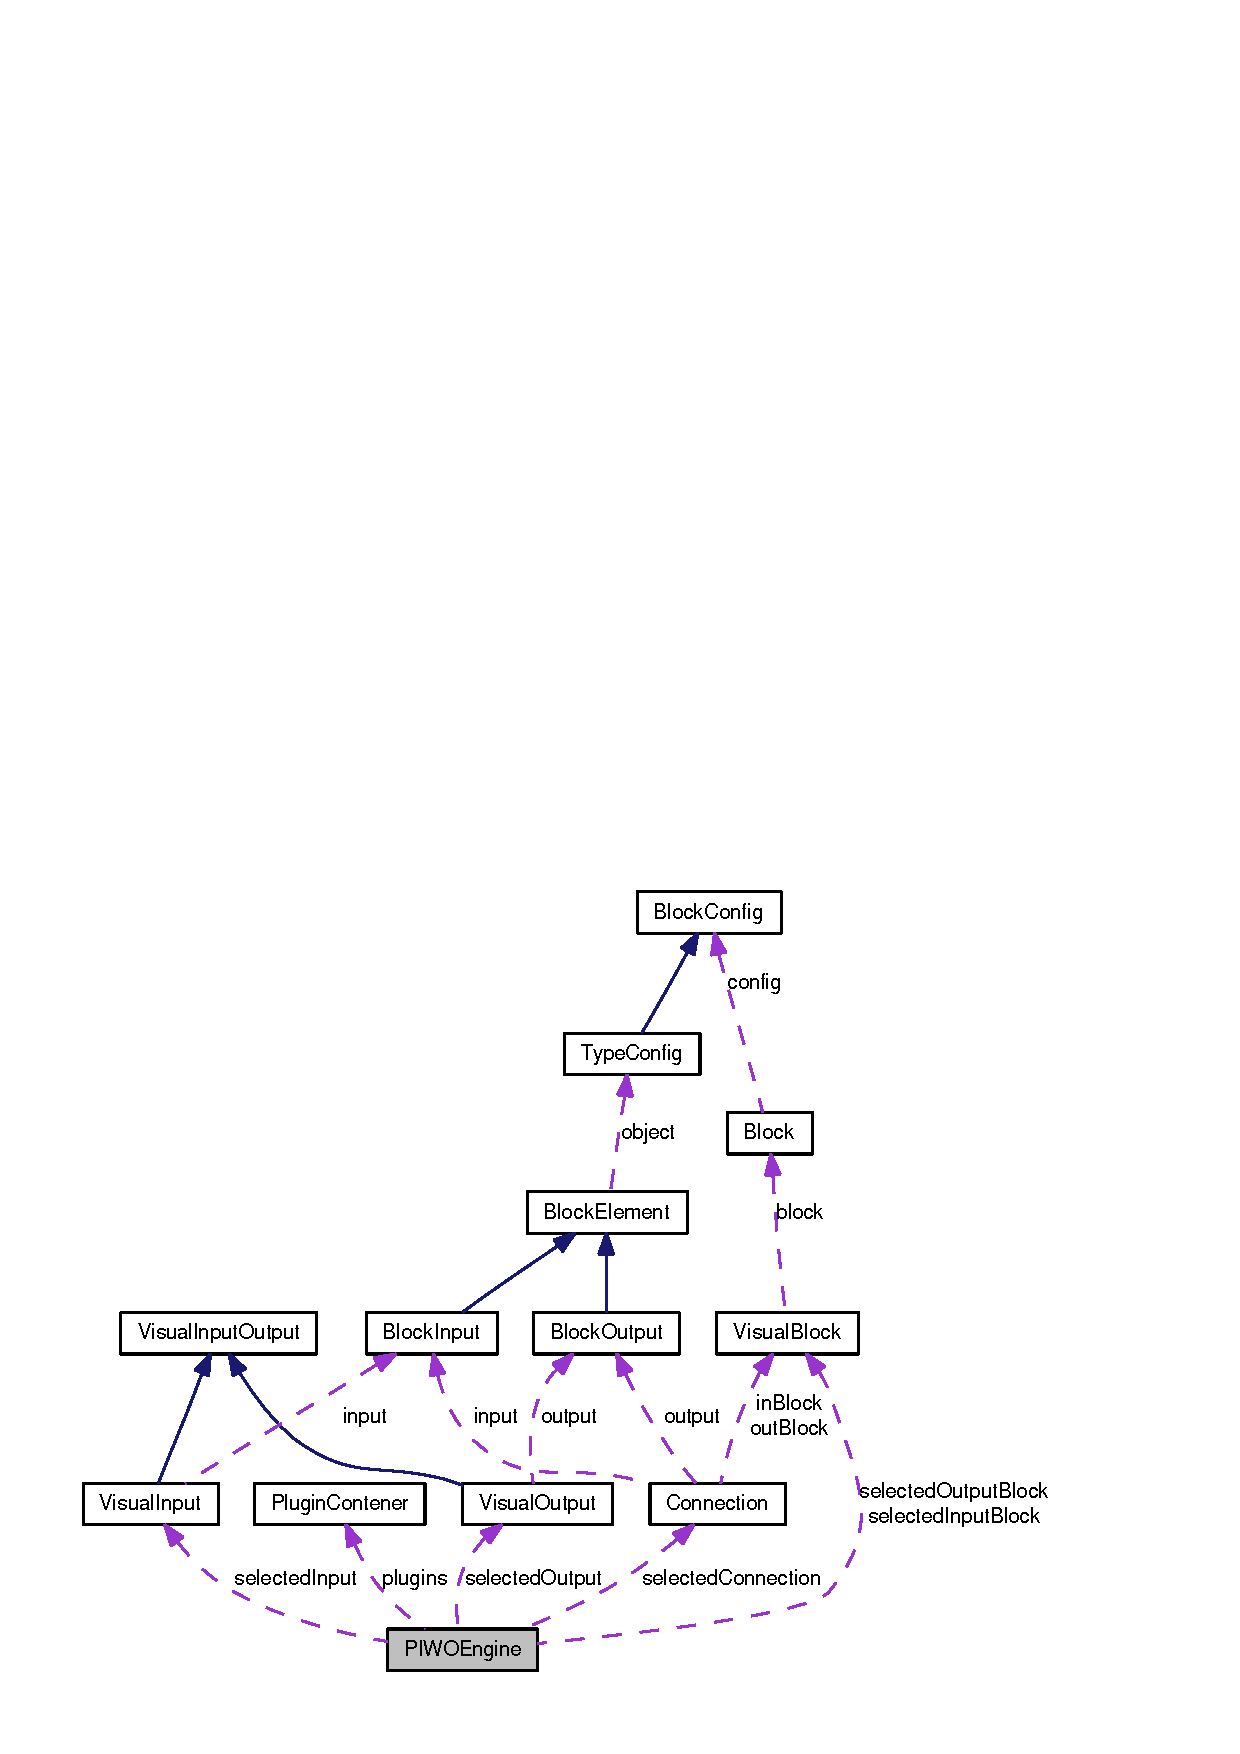
\includegraphics[width=400pt]{classPIWOEngine__coll__graph}
\end{center}
\end{figure}
\subsection*{Public Member Functions}
\begin{CompactItemize}
\item 
\_\-\_\-fastcall \hyperlink{classPIWOEngine_cdfa1d8927a1dec652d405c4f6162f19}{PIWOEngine} (TComponent $\ast$Owner)
\item 
\_\-\_\-fastcall \hyperlink{classPIWOEngine_e7b0e23554e0bbac03efece62653e69f}{$\sim$PIWOEngine} ()
\item 
bool \hyperlink{classPIWOEngine_36ccc94c01c411c848b08900254caf70}{AddBlock} (const AnsiString \&name)
\item 
bool \hyperlink{classPIWOEngine_d55f140db8722ff1601fa675ec779e1d}{DeleteBlock} (const AnsiString \&fullName)
\item 
bool \hyperlink{classPIWOEngine_a11ad8ce77d2e5b026ebc3469bdff0d9}{DeleteSelectedBlocks} ()
\item 
bool \hyperlink{classPIWOEngine_edd85509770c459cd621bfeb5eba4ac7}{DeleteAllBlocks} ()
\item 
void \hyperlink{classPIWOEngine_27e53e5d565cca55d8663a14906ab720}{SelectAllBlocks} ()
\item 
void \hyperlink{classPIWOEngine_b8926ec72c402ff687ac16061c9d35eb}{InvertBlockSelection} ()
\item 
void \hyperlink{classPIWOEngine_60d90f58e1d47c5a12547126700799c7}{UnselectAllBlocks} ()
\item 
bool \hyperlink{classPIWOEngine_60f3cba63905531e827476ad139ddf62}{DeleteSelectedConnection} ()
\item 
bool \hyperlink{classPIWOEngine_93143ee719ccb9645a8d9c197f4fc7b0}{DeleteAllConnections} ()
\item 
void \hyperlink{classPIWOEngine_2ec5c192d058a7a44ab82a30fa331c99}{UnselectSelectedConnection} ()
\item 
void \hyperlink{classPIWOEngine_2e52cfe4cc826cd43595ca9c7ae979f9}{CancelCustomizationOnSelectedConnections} ()
\item 
void \hyperlink{classPIWOEngine_0e28412b868f3042c7bf50e9ee8c40fc}{CancelCustomizationOnAllConnections} ()
\item 
void \hyperlink{classPIWOEngine_6e37ad69880f3d9a9ad7cf9b57d894a9}{DuplcateSelectedBlocks} ()
\item 
void \hyperlink{classPIWOEngine_3585d1f4c45df99a02c36af9cab8e343}{validateAll} ()
\item 
bool \hyperlink{classPIWOEngine_d20139057c6b68e8e4e2fb0d0e04926b}{run} (bool useHistory=true)
\item 
bool \hyperlink{classPIWOEngine_b8cd8305728eb8998011af59677084ad}{isRuned} ()
\item 
void \hyperlink{classPIWOEngine_134ab9db62730d3a680f24bf33068672}{abort} (bool wait=false)
\item 
bool \hyperlink{classPIWOEngine_8505bb4deb5c952d8f93d5b656f385cf}{isAborted} ()
\item 
bool \hyperlink{classPIWOEngine_dee854cac7e50d95de9613e2bbdb4676}{saveToFile} (const AnsiString \&filename)
\item 
bool \hyperlink{classPIWOEngine_84deceb11d30a25d104a2b34afad27d4}{loadFromFile} (const AnsiString \&filename)
\item 
bool \hyperlink{classPIWOEngine_994cb25914cba46f02bdf14909991247}{isChanged} ()
\item 
int \hyperlink{classPIWOEngine_070ee971be58a47520dd7e5063e5508e}{getBlockCount} ()
\item 
int \hyperlink{classPIWOEngine_1c1eb9af5a92cf907bdce516de31af37}{getConnectionsCount} ()
\item 
bool \hyperlink{classPIWOEngine_ff65b56ee08c0ccbdd9724ebc08dc2ad}{isBlockSelected} ()
\item 
bool \hyperlink{classPIWOEngine_7bd61a1844a459b79a07a3ecf08d72a3}{isConnectionSelected} ()
\end{CompactItemize}
\subsection*{Public Attributes}
\begin{CompactItemize}
\item 
Graphics::TBitmap $\ast$ \hyperlink{classPIWOEngine_23d5dbc92608ee42ba7975d2454ecbcf}{defaultBlockImage}
\item 
PIWOEngine\_\-Log \hyperlink{classPIWOEngine_e5b5e665729db134c485ff27305b7888}{OnInformation}
\item 
PIWOEngine\_\-Log \hyperlink{classPIWOEngine_52bbb80846422f21ab9b03d67ad67a60}{OnDebug}
\item 
PIWOEngine\_\-Log \hyperlink{classPIWOEngine_37a8c63dad516bc24be59cdca3a1eaa6}{OnSuccess}
\item 
PIWOEngine\_\-Log \hyperlink{classPIWOEngine_c7a83bdff3736e35b68584bcb3a4b699}{OnWarrning}
\item 
PIWOEngine\_\-Log \hyperlink{classPIWOEngine_55424b81f56591f23f3b58e0fdd399d2}{OnError}
\item 
PIWOEngine\_\-Log \hyperlink{classPIWOEngine_02e912fd9ead4eabd48b32f769bd77c1}{OnRunInformation}
\item 
PIWOEngine\_\-Log \hyperlink{classPIWOEngine_cc1ea09371765860dfc2912dc605f9be}{OnRunDebug}
\item 
PIWOEngine\_\-Log \hyperlink{classPIWOEngine_faa892e8c9a1a5973a300d2f02143897}{OnRunSuccess}
\item 
PIWOEngine\_\-Log \hyperlink{classPIWOEngine_ede20b6476b9e1d0db96878e2eee4481}{OnRunWarrning}
\item 
PIWOEngine\_\-Log \hyperlink{classPIWOEngine_303f960016f76986cba65e2c0aaea4e1}{OnRunError}
\item 
PIWOEngine\_\-Event \hyperlink{classPIWOEngine_ed5f12ba5e4872c5326126080a2cd821}{OnBlockSelected}
\item 
PIWOEngine\_\-Event \hyperlink{classPIWOEngine_45e9d4a676e2c489718b23491af65206}{OnConnectionSelected}
\item 
PIWOEngine\_\-Event \hyperlink{classPIWOEngine_df70bc69dc41278c1d2b02f308a1ba20}{OnNothingSelected}
\item 
PIWOEngine\_\-Event \hyperlink{classPIWOEngine_5322d9b9def723ae036b005c5a3c578e}{OnChanged}
\item 
\hyperlink{PIWOEngine_8h_8273eb67828fc9cc4e2b18b930dada38}{PIWOEngine\_\-RunProgress} \hyperlink{classPIWOEngine_c300fdccbd5cf4fa9ad200d10856fd3b}{OnRunProgress}
\item 
PIWOEngine\_\-Event \hyperlink{classPIWOEngine_b5d044c03265cf49fc87e58cd2134749}{OnRunStart}
\item 
PIWOEngine\_\-Event \hyperlink{classPIWOEngine_7de6e8504739db45b1ba5defeb63d80c}{OnRunEnd}
\item 
\hyperlink{classPluginContener}{PluginContener} $\ast$ \hyperlink{classPIWOEngine_6433fe1909e1f8fdecd7ebc9cc0ec4a3}{plugins}
\item 
vector$<$ \hyperlink{classTHistory}{THistory} $\ast$ $>$ \hyperlink{classPIWOEngine_dd08ebde966bf33e79750fb1b1dcca08}{historyWindows}
\item 
bool \hyperlink{classPIWOEngine_5730b8e65319ad792660fa205495f298}{alwaysRun}
\end{CompactItemize}
\subsection*{Private Member Functions}
\begin{CompactItemize}
\item 
void \hyperlink{classPIWOEngine_97f4f39393b6fc49fe33b867b46b9564}{OnVisualBlockConfigClick} (TObject $\ast$Sender)
\item 
void \hyperlink{classPIWOEngine_4e51d927289a1bcb9dc8f1153d457e93}{OnVisualBlockInputSelected} (\hyperlink{classVisualInput}{VisualInput} $\ast$input, TObject $\ast$Sender)
\item 
void \hyperlink{classPIWOEngine_0b7e4c9ee82bab94f35d8cc5f6cda3f7}{OnVisualBlockOutputSelected} (\hyperlink{classVisualOutput}{VisualOutput} $\ast$output, TObject $\ast$Sender)
\item 
void \hyperlink{classPIWOEngine_1a54c292b17426a1690de0500a72d8fa}{OnVisualBlockInputHistoryClick} (\hyperlink{classVisualInput}{VisualInput} $\ast$input, TObject $\ast$Sender)
\item 
void \hyperlink{classPIWOEngine_32a93f8cc49a3c9988674e99765d9cee}{OnVisualBlockOutputHistoryClick} (\hyperlink{classVisualOutput}{VisualOutput} $\ast$output, TObject $\ast$Sender)
\item 
void \hyperlink{classPIWOEngine_07f70dcb30a6077266626c7f52ce1667}{OnVisualBlockMove} (TObject $\ast$Sender, bool moveAll, int x, int y)
\item 
void \hyperlink{classPIWOEngine_2baa1b7c8bb6b91e413b8cc2a7f5b8ea}{OnVisualBlockUnselect} (TObject $\ast$Sender)
\item 
void \hyperlink{classPIWOEngine_94a545e2d82c78fffc68c79f53db4a72}{OnVisualBlockSelect} (TObject $\ast$Sender)
\item 
void \hyperlink{classPIWOEngine_7ec3c8295c1984c7661c813881fb5bda}{OnVisualBlockSelectAdd} (TObject $\ast$Sender)
\item 
void \_\-\_\-fastcall \hyperlink{classPIWOEngine_c0f3009bc8be06d0242546f8a2e6fc94}{onThisClick} (TObject $\ast$Sender)
\item 
void \hyperlink{classPIWOEngine_1a8f4608620d249e9982004773bf1fe9}{OnConnectionSelect} (void $\ast$Sender)
\item 
void \_\-\_\-fastcall \hyperlink{classPIWOEngine_deb8c8ae4c4d5f69c242f222dc2557bb}{HistoryFormClose} (TObject $\ast$Sender, TCloseAction \&Action)
\item 
void \hyperlink{classPIWOEngine_9e8cffc64037b892fbdb1daf3459a31d}{validateBlock} (\hyperlink{classVisualBlock}{VisualBlock} $\ast$block, bool updateInputConnections=true)
\item 
\hyperlink{classConnection}{Connection} $\ast$ \hyperlink{classPIWOEngine_7d7bed1c6a1f91bd7c3c4ca7ac696bc9}{getConnectionTo} (\hyperlink{classVisualInput}{VisualInput} $\ast$input)
\item 
bool \hyperlink{classPIWOEngine_e993fd1568a25f8ce5e3719212871ae5}{MakeConnection} (\hyperlink{classVisualBlock}{VisualBlock} $\ast$outputBlock, \hyperlink{classVisualOutput}{VisualOutput} $\ast$output, \hyperlink{classVisualBlock}{VisualBlock} $\ast$inputBlock, \hyperlink{classVisualInput}{VisualInput} $\ast$input)
\item 
bool \hyperlink{classPIWOEngine_ea240e8aed286fe05d3baf086d9d9c85}{runBlock} (\hyperlink{classVisualBlock}{VisualBlock} $\ast$block, bool fastRun, bool $\ast$useHistory)
\item 
bool \hyperlink{classPIWOEngine_f4a1573d29015d4fa8c1a1e37df86de3}{runUsingHistory} ()
\item 
bool \hyperlink{classPIWOEngine_302753a45663305fcef14a5c8c348a02}{runNotUsingHistory} ()
\end{CompactItemize}
\subsection*{Private Attributes}
\begin{CompactItemize}
\item 
PIWOMAINCLASSTYPE $\ast$ \hyperlink{classPIWOEngine_d5da32bb11409879f33eca9ebddfc9d6}{area}
\item 
vector$<$ \hyperlink{classVisualBlock}{VisualBlock} $\ast$ $>$ \hyperlink{classPIWOEngine_8cc6b573d0eacacc5043891a36b6e820}{blocks}
\item 
vector$<$ \hyperlink{classConnection}{Connection} $\ast$ $>$ \hyperlink{classPIWOEngine_192e9886f89d0eee49173cc199afe561}{connections}
\item 
\hyperlink{classConnection}{Connection} $\ast$ \hyperlink{classPIWOEngine_89b3e231d010fe4a3672704b68e9fcea}{selectedConnection}
\item 
vector$<$ \hyperlink{classVisualBlock}{VisualBlock} $\ast$ $>$ \hyperlink{classPIWOEngine_c2cf186bc174d18bc9764b534bb5879d}{selectedBlocks}
\item 
\hyperlink{classVisualBlock}{VisualBlock} $\ast$ \hyperlink{classPIWOEngine_573250b25797190affc38e1e3fdf8bf3}{selectedOutputBlock}
\item 
\hyperlink{classVisualBlock}{VisualBlock} $\ast$ \hyperlink{classPIWOEngine_9fe3dcb62ef1ef7860afe06ddca01585}{selectedInputBlock}
\item 
\hyperlink{classVisualInput}{VisualInput} $\ast$ \hyperlink{classPIWOEngine_87ae251a3b1c318e8c26e85396fde9e9}{selectedInput}
\item 
\hyperlink{classVisualOutput}{VisualOutput} $\ast$ \hyperlink{classPIWOEngine_3008a57c7914a602b34bf470a90d2bb6}{selectedOutput}
\item 
bool \hyperlink{classPIWOEngine_58d8519fdc284ac5b088d4b9ead41de1}{isRunning}
\item 
bool \hyperlink{classPIWOEngine_fb15e05147a0a299649307876eb97412}{stopRunning}
\item 
unsigned int \hyperlink{classPIWOEngine_84d4db25d471839e7cdd44ae0eb2b517}{runProgress}
\item 
bool \hyperlink{classPIWOEngine_3d5702db522458d8de52d3dbd0203cdc}{changed}
\end{CompactItemize}


\subsection{Detailed Description}
Glowna klasa projektu, kazda jej instancja symbolizuje osobny projekt 

Definition at line 21 of file PIWOEngine.h.

\subsection{Constructor \& Destructor Documentation}
\hypertarget{classPIWOEngine_cdfa1d8927a1dec652d405c4f6162f19}{
\index{PIWOEngine@{PIWOEngine}!PIWOEngine@{PIWOEngine}}
\index{PIWOEngine@{PIWOEngine}!PIWOEngine@{PIWOEngine}}
\subsubsection[PIWOEngine]{\setlength{\rightskip}{0pt plus 5cm}\_\-\_\-fastcall PIWOEngine::PIWOEngine (TComponent $\ast$ {\em Owner})}}
\label{classPIWOEngine_cdfa1d8927a1dec652d405c4f6162f19}


Konstruktor \begin{Desc}
\item[Parameters:]
\begin{description}
\item[{\em Owner}]komponent bedacy parentem i wlascicielem dla projektu \end{description}
\end{Desc}


Definition at line 8 of file PIWOEngine.cpp.

References alwaysRun, area, changed, defaultBlockImage, isRunning, OnBlockSelected, OnConnectionSelected, OnDebug, OnError, OnInformation, OnNothingSelected, OnRunDebug, OnRunEnd, OnRunError, OnRunInformation, OnRunProgress, OnRunStart, OnRunSuccess, OnRunWarrning, OnSuccess, onThisClick(), OnWarrning, PIWOMAINCLASSTYPE, plugins, runProgress, selectedConnection, selectedInput, selectedInputBlock, selectedOutput, selectedOutputBlock, and stopRunning.\hypertarget{classPIWOEngine_e7b0e23554e0bbac03efece62653e69f}{
\index{PIWOEngine@{PIWOEngine}!$\sim$PIWOEngine@{$\sim$PIWOEngine}}
\index{$\sim$PIWOEngine@{$\sim$PIWOEngine}!PIWOEngine@{PIWOEngine}}
\subsubsection[$\sim$PIWOEngine]{\setlength{\rightskip}{0pt plus 5cm}\_\-\_\-fastcall PIWOEngine::$\sim$PIWOEngine ()}}
\label{classPIWOEngine_e7b0e23554e0bbac03efece62653e69f}


Destruktor 

Definition at line 61 of file PIWOEngine.cpp.

References area, blocks, connections, and historyWindows.

\subsection{Member Function Documentation}
\hypertarget{classPIWOEngine_97f4f39393b6fc49fe33b867b46b9564}{
\index{PIWOEngine@{PIWOEngine}!OnVisualBlockConfigClick@{OnVisualBlockConfigClick}}
\index{OnVisualBlockConfigClick@{OnVisualBlockConfigClick}!PIWOEngine@{PIWOEngine}}
\subsubsection[OnVisualBlockConfigClick]{\setlength{\rightskip}{0pt plus 5cm}void PIWOEngine::OnVisualBlockConfigClick (TObject $\ast$ {\em Sender})\hspace{0.3cm}{\tt  \mbox{[}private\mbox{]}}}}
\label{classPIWOEngine_97f4f39393b6fc49fe33b867b46b9564}




Definition at line 397 of file PIWOEngine.cpp.

References abort(), alwaysRun, VisualBlock::block, changed, Block::getConfig(), PluginContener::getFunction(), BlockConfig::getRevision(), VisualBlock::getTitle(), VisualBlock::nameOfBlock, OnChanged, OnDebug, OnError, OnWarrning, plugins, run(), FunctionDLL::showConfig(), and validateBlock().

Referenced by AddBlock(), DuplcateSelectedBlocks(), and loadFromFile().\hypertarget{classPIWOEngine_4e51d927289a1bcb9dc8f1153d457e93}{
\index{PIWOEngine@{PIWOEngine}!OnVisualBlockInputSelected@{OnVisualBlockInputSelected}}
\index{OnVisualBlockInputSelected@{OnVisualBlockInputSelected}!PIWOEngine@{PIWOEngine}}
\subsubsection[OnVisualBlockInputSelected]{\setlength{\rightskip}{0pt plus 5cm}void PIWOEngine::OnVisualBlockInputSelected ({\bf VisualInput} $\ast$ {\em input}, \/  TObject $\ast$ {\em Sender})\hspace{0.3cm}{\tt  \mbox{[}private\mbox{]}}}}
\label{classPIWOEngine_4e51d927289a1bcb9dc8f1153d457e93}




Definition at line 529 of file PIWOEngine.cpp.

References abort(), alwaysRun, changed, connections, BlockInput::disconnect(), getConnectionTo(), BlockElement::getDescription(), VisualBlock::getTitle(), Connection::inBlock, Connection::input, MakeConnection(), OnChanged, Connection::outBlock, VisualOutput::output, Connection::output, run(), selectedInput, selectedInputBlock, selectedOutput, selectedOutputBlock, and validateBlock().

Referenced by AddBlock(), DuplcateSelectedBlocks(), and loadFromFile().\hypertarget{classPIWOEngine_0b7e4c9ee82bab94f35d8cc5f6cda3f7}{
\index{PIWOEngine@{PIWOEngine}!OnVisualBlockOutputSelected@{OnVisualBlockOutputSelected}}
\index{OnVisualBlockOutputSelected@{OnVisualBlockOutputSelected}!PIWOEngine@{PIWOEngine}}
\subsubsection[OnVisualBlockOutputSelected]{\setlength{\rightskip}{0pt plus 5cm}void PIWOEngine::OnVisualBlockOutputSelected ({\bf VisualOutput} $\ast$ {\em output}, \/  TObject $\ast$ {\em Sender})\hspace{0.3cm}{\tt  \mbox{[}private\mbox{]}}}}
\label{classPIWOEngine_0b7e4c9ee82bab94f35d8cc5f6cda3f7}




Definition at line 598 of file PIWOEngine.cpp.

References abort(), alwaysRun, changed, connections, BlockInput::disconnect(), getConnectionTo(), BlockElement::getDescription(), VisualBlock::getTitle(), Connection::inBlock, Connection::input, MakeConnection(), OnChanged, Connection::outBlock, VisualOutput::output, Connection::output, run(), selectedInput, selectedInputBlock, selectedOutput, selectedOutputBlock, and validateBlock().

Referenced by AddBlock(), DuplcateSelectedBlocks(), and loadFromFile().\hypertarget{classPIWOEngine_1a54c292b17426a1690de0500a72d8fa}{
\index{PIWOEngine@{PIWOEngine}!OnVisualBlockInputHistoryClick@{OnVisualBlockInputHistoryClick}}
\index{OnVisualBlockInputHistoryClick@{OnVisualBlockInputHistoryClick}!PIWOEngine@{PIWOEngine}}
\subsubsection[OnVisualBlockInputHistoryClick]{\setlength{\rightskip}{0pt plus 5cm}void PIWOEngine::OnVisualBlockInputHistoryClick ({\bf VisualInput} $\ast$ {\em input}, \/  TObject $\ast$ {\em Sender})\hspace{0.3cm}{\tt  \mbox{[}private\mbox{]}}}}
\label{classPIWOEngine_1a54c292b17426a1690de0500a72d8fa}




Definition at line 679 of file PIWOEngine.cpp.

References THistory::block, BlockElement::getDescription(), BlockElement::getName(), VisualBlock::getTitle(), VisualBlock::history, HistoryFormClose(), historyWindows, VisualInput::input, OnDebug, OnWarrning, plugins, THistory::plugins, and THistory::refresh().

Referenced by AddBlock(), DuplcateSelectedBlocks(), and loadFromFile().\hypertarget{classPIWOEngine_32a93f8cc49a3c9988674e99765d9cee}{
\index{PIWOEngine@{PIWOEngine}!OnVisualBlockOutputHistoryClick@{OnVisualBlockOutputHistoryClick}}
\index{OnVisualBlockOutputHistoryClick@{OnVisualBlockOutputHistoryClick}!PIWOEngine@{PIWOEngine}}
\subsubsection[OnVisualBlockOutputHistoryClick]{\setlength{\rightskip}{0pt plus 5cm}void PIWOEngine::OnVisualBlockOutputHistoryClick ({\bf VisualOutput} $\ast$ {\em output}, \/  TObject $\ast$ {\em Sender})\hspace{0.3cm}{\tt  \mbox{[}private\mbox{]}}}}
\label{classPIWOEngine_32a93f8cc49a3c9988674e99765d9cee}




Definition at line 713 of file PIWOEngine.cpp.

References THistory::block, BlockElement::getDescription(), BlockElement::getName(), VisualBlock::getTitle(), VisualBlock::history, HistoryFormClose(), historyWindows, OnDebug, OnWarrning, VisualOutput::output, plugins, THistory::plugins, and THistory::refresh().

Referenced by AddBlock(), DuplcateSelectedBlocks(), and loadFromFile().\hypertarget{classPIWOEngine_07f70dcb30a6077266626c7f52ce1667}{
\index{PIWOEngine@{PIWOEngine}!OnVisualBlockMove@{OnVisualBlockMove}}
\index{OnVisualBlockMove@{OnVisualBlockMove}!PIWOEngine@{PIWOEngine}}
\subsubsection[OnVisualBlockMove]{\setlength{\rightskip}{0pt plus 5cm}void PIWOEngine::OnVisualBlockMove (TObject $\ast$ {\em Sender}, \/  bool {\em moveAll}, \/  int {\em x}, \/  int {\em y})\hspace{0.3cm}{\tt  \mbox{[}private\mbox{]}}}}
\label{classPIWOEngine_07f70dcb30a6077266626c7f52ce1667}




Definition at line 747 of file PIWOEngine.cpp.

References changed, connections, OnChanged, and selectedBlocks.

Referenced by AddBlock(), DuplcateSelectedBlocks(), and loadFromFile().\hypertarget{classPIWOEngine_2baa1b7c8bb6b91e413b8cc2a7f5b8ea}{
\index{PIWOEngine@{PIWOEngine}!OnVisualBlockUnselect@{OnVisualBlockUnselect}}
\index{OnVisualBlockUnselect@{OnVisualBlockUnselect}!PIWOEngine@{PIWOEngine}}
\subsubsection[OnVisualBlockUnselect]{\setlength{\rightskip}{0pt plus 5cm}void PIWOEngine::OnVisualBlockUnselect (TObject $\ast$ {\em Sender})\hspace{0.3cm}{\tt  \mbox{[}private\mbox{]}}}}
\label{classPIWOEngine_2baa1b7c8bb6b91e413b8cc2a7f5b8ea}




Definition at line 793 of file PIWOEngine.cpp.

References VisualBlock::getTitle(), OnBlockSelected, OnConnectionSelected, OnDebug, OnNothingSelected, selectedBlocks, selectedConnection, and VisualBlock::setSelected().

Referenced by AddBlock(), DuplcateSelectedBlocks(), and loadFromFile().\hypertarget{classPIWOEngine_94a545e2d82c78fffc68c79f53db4a72}{
\index{PIWOEngine@{PIWOEngine}!OnVisualBlockSelect@{OnVisualBlockSelect}}
\index{OnVisualBlockSelect@{OnVisualBlockSelect}!PIWOEngine@{PIWOEngine}}
\subsubsection[OnVisualBlockSelect]{\setlength{\rightskip}{0pt plus 5cm}void PIWOEngine::OnVisualBlockSelect (TObject $\ast$ {\em Sender})\hspace{0.3cm}{\tt  \mbox{[}private\mbox{]}}}}
\label{classPIWOEngine_94a545e2d82c78fffc68c79f53db4a72}




Definition at line 815 of file PIWOEngine.cpp.

References connections, OnBlockSelected, OnConnectionSelected, OnDebug, OnNothingSelected, selectedBlocks, selectedConnection, and UnselectSelectedConnection().

Referenced by AddBlock(), DuplcateSelectedBlocks(), and loadFromFile().\hypertarget{classPIWOEngine_7ec3c8295c1984c7661c813881fb5bda}{
\index{PIWOEngine@{PIWOEngine}!OnVisualBlockSelectAdd@{OnVisualBlockSelectAdd}}
\index{OnVisualBlockSelectAdd@{OnVisualBlockSelectAdd}!PIWOEngine@{PIWOEngine}}
\subsubsection[OnVisualBlockSelectAdd]{\setlength{\rightskip}{0pt plus 5cm}void PIWOEngine::OnVisualBlockSelectAdd (TObject $\ast$ {\em Sender})\hspace{0.3cm}{\tt  \mbox{[}private\mbox{]}}}}
\label{classPIWOEngine_7ec3c8295c1984c7661c813881fb5bda}




Definition at line 844 of file PIWOEngine.cpp.

References connections, OnBlockSelected, OnConnectionSelected, OnDebug, OnNothingSelected, selectedBlocks, selectedConnection, and UnselectSelectedConnection().

Referenced by AddBlock(), DuplcateSelectedBlocks(), and loadFromFile().\hypertarget{classPIWOEngine_c0f3009bc8be06d0242546f8a2e6fc94}{
\index{PIWOEngine@{PIWOEngine}!onThisClick@{onThisClick}}
\index{onThisClick@{onThisClick}!PIWOEngine@{PIWOEngine}}
\subsubsection[onThisClick]{\setlength{\rightskip}{0pt plus 5cm}void \_\-\_\-fastcall PIWOEngine::onThisClick (TObject $\ast$ {\em Sender})\hspace{0.3cm}{\tt  \mbox{[}private\mbox{]}}}}
\label{classPIWOEngine_c0f3009bc8be06d0242546f8a2e6fc94}




Definition at line 869 of file PIWOEngine.cpp.

References UnselectAllBlocks(), and UnselectSelectedConnection().

Referenced by PIWOEngine().\hypertarget{classPIWOEngine_1a8f4608620d249e9982004773bf1fe9}{
\index{PIWOEngine@{PIWOEngine}!OnConnectionSelect@{OnConnectionSelect}}
\index{OnConnectionSelect@{OnConnectionSelect}!PIWOEngine@{PIWOEngine}}
\subsubsection[OnConnectionSelect]{\setlength{\rightskip}{0pt plus 5cm}void PIWOEngine::OnConnectionSelect (void $\ast$ {\em Sender})\hspace{0.3cm}{\tt  \mbox{[}private\mbox{]}}}}
\label{classPIWOEngine_1a8f4608620d249e9982004773bf1fe9}




Definition at line 875 of file PIWOEngine.cpp.

References Connection::BringToFront(), BlockElement::getDescription(), VisualBlock::getTitle(), Connection::inBlock, Connection::input, OnBlockSelected, OnConnectionSelected, OnDebug, OnNothingSelected, Connection::outBlock, Connection::output, selectedBlocks, selectedConnection, Connection::setSelected(), and UnselectAllBlocks().

Referenced by DuplcateSelectedBlocks(), loadFromFile(), and MakeConnection().\hypertarget{classPIWOEngine_deb8c8ae4c4d5f69c242f222dc2557bb}{
\index{PIWOEngine@{PIWOEngine}!HistoryFormClose@{HistoryFormClose}}
\index{HistoryFormClose@{HistoryFormClose}!PIWOEngine@{PIWOEngine}}
\subsubsection[HistoryFormClose]{\setlength{\rightskip}{0pt plus 5cm}void \_\-\_\-fastcall PIWOEngine::HistoryFormClose (TObject $\ast$ {\em Sender}, \/  TCloseAction \& {\em Action})\hspace{0.3cm}{\tt  \mbox{[}private\mbox{]}}}}
\label{classPIWOEngine_deb8c8ae4c4d5f69c242f222dc2557bb}




Definition at line 665 of file PIWOEngine.cpp.

References historyWindows, and OnDebug.

Referenced by OnVisualBlockInputHistoryClick(), and OnVisualBlockOutputHistoryClick().\hypertarget{classPIWOEngine_9e8cffc64037b892fbdb1daf3459a31d}{
\index{PIWOEngine@{PIWOEngine}!validateBlock@{validateBlock}}
\index{validateBlock@{validateBlock}!PIWOEngine@{PIWOEngine}}
\subsubsection[validateBlock]{\setlength{\rightskip}{0pt plus 5cm}void PIWOEngine::validateBlock ({\bf VisualBlock} $\ast$ {\em block}, \/  bool {\em updateInputConnections} = {\tt true})\hspace{0.3cm}{\tt  \mbox{[}private\mbox{]}}}}
\label{classPIWOEngine_9e8cffc64037b892fbdb1daf3459a31d}




Definition at line 146 of file PIWOEngine.cpp.

References VisualBlock::block, changed, BlockValidateInputElement::connection, BlockValidateOutputElement::connections, connections, BlockValidateOutputElement::errorCode, BlockValidateInputElement::errorCode, BlockValidateOutputElement::errorDescription, BlockValidateInputElement::errorDescription, BlockElement::getErrorCode(), BlockElement::getErrorDescription(), PluginContener::getFunction(), BlockOutput::getOutputType(), VisualBlock::getTitle(), BlockValidateInputElement::input, Block::input, VisualBlock::nameOfBlock, OnChanged, OnDebug, OnError, BlockValidateOutputElement::output, Block::output, plugins, BlockValidateOutputElement::type, VisualBlock::updateHistory(), and VisualBlock::updateVisualComponents().

Referenced by AddBlock(), DeleteAllConnections(), DeleteBlock(), DeleteSelectedBlocks(), DeleteSelectedConnection(), DuplcateSelectedBlocks(), loadFromFile(), MakeConnection(), OnVisualBlockConfigClick(), OnVisualBlockInputSelected(), OnVisualBlockOutputSelected(), and validateAll().\hypertarget{classPIWOEngine_7d7bed1c6a1f91bd7c3c4ca7ac696bc9}{
\index{PIWOEngine@{PIWOEngine}!getConnectionTo@{getConnectionTo}}
\index{getConnectionTo@{getConnectionTo}!PIWOEngine@{PIWOEngine}}
\subsubsection[getConnectionTo]{\setlength{\rightskip}{0pt plus 5cm}{\bf Connection} $\ast$ PIWOEngine::getConnectionTo ({\bf VisualInput} $\ast$ {\em input})\hspace{0.3cm}{\tt  \mbox{[}private\mbox{]}}}}
\label{classPIWOEngine_7d7bed1c6a1f91bd7c3c4ca7ac696bc9}




Definition at line 895 of file PIWOEngine.cpp.

References connections, and VisualInput::input.

Referenced by OnVisualBlockInputSelected(), and OnVisualBlockOutputSelected().\hypertarget{classPIWOEngine_e993fd1568a25f8ce5e3719212871ae5}{
\index{PIWOEngine@{PIWOEngine}!MakeConnection@{MakeConnection}}
\index{MakeConnection@{MakeConnection}!PIWOEngine@{PIWOEngine}}
\subsubsection[MakeConnection]{\setlength{\rightskip}{0pt plus 5cm}bool PIWOEngine::MakeConnection ({\bf VisualBlock} $\ast$ {\em outputBlock}, \/  {\bf VisualOutput} $\ast$ {\em output}, \/  {\bf VisualBlock} $\ast$ {\em inputBlock}, \/  {\bf VisualInput} $\ast$ {\em input})\hspace{0.3cm}{\tt  \mbox{[}private\mbox{]}}}}
\label{classPIWOEngine_e993fd1568a25f8ce5e3719212871ae5}




Definition at line 439 of file PIWOEngine.cpp.

References BlockInput::allowedTypes, area, changed, BlockInput::connect(), connections, Connection::draw(), BlockElement::getDescription(), BlockOutput::getOutputType(), VisualBlock::getTitle(), Connection::inBlock, Connection::input, VisualInput::input, OnBlockSelected, OnChanged, OnConnectionSelect(), OnConnectionSelected, Connection::OnConnectionSelected, OnDebug, OnError, OnInformation, OnNothingSelected, Connection::outBlock, Connection::output, VisualOutput::output, selectedBlocks, selectedConnection, Connection::setSelected(), Connection::update(), and validateBlock().

Referenced by OnVisualBlockInputSelected(), and OnVisualBlockOutputSelected().\hypertarget{classPIWOEngine_ea240e8aed286fe05d3baf086d9d9c85}{
\index{PIWOEngine@{PIWOEngine}!runBlock@{runBlock}}
\index{runBlock@{runBlock}!PIWOEngine@{PIWOEngine}}
\subsubsection[runBlock]{\setlength{\rightskip}{0pt plus 5cm}bool PIWOEngine::runBlock ({\bf VisualBlock} $\ast$ {\em block}, \/  bool {\em fastRun}, \/  bool $\ast$ {\em useHistory})\hspace{0.3cm}{\tt  \mbox{[}private\mbox{]}}}}
\label{classPIWOEngine_ea240e8aed286fe05d3baf086d9d9c85}




Definition at line 1500 of file PIWOEngine.cpp.

References VisualBlock::block, blocks, BlockHistory::bottomOutput, VisualBlock::bottomOutput, BlockHistory::configRevision, connections, Block::getConfig(), PluginContener::getFunction(), TypeConfig::getName(), BlockElement::getObject(), BlockConfig::getRevision(), VisualBlock::getTitle(), PluginContener::getType(), TypeDLL::getType(), VisualBlock::history, historyWindows, BlockHistoryInputElement::input, Block::input, TypeDLL::isValid(), BlockHistory::leftInput, VisualBlock::leftInput, VisualBlock::nameOfBlock, OnError, OnRunDebug, OnRunError, OnRunInformation, OnRunProgress, OnRunSuccess, OnRunWarrning, Connection::outBlock, BlockHistoryOutputElement::output, Block::output, Connection::output, plugins, BlockHistory::rightOutput, VisualBlock::rightOutput, FunctionDLL::run(), VisualBlock::runned, runProgress, BlockHistoryOutputElement::setData(), BlockHistoryInputElement::setData(), BlockHistoryOutputElement::setNULL(), BlockHistoryInputElement::setNULL(), VisualBlock::setStatusColor(), stopRunning, BlockHistory::topInput, VisualBlock::topInput, Connection::update(), and VisualBlock::updateVisualComponents().

Referenced by runNotUsingHistory(), and runUsingHistory().\hypertarget{classPIWOEngine_f4a1573d29015d4fa8c1a1e37df86de3}{
\index{PIWOEngine@{PIWOEngine}!runUsingHistory@{runUsingHistory}}
\index{runUsingHistory@{runUsingHistory}!PIWOEngine@{PIWOEngine}}
\subsubsection[runUsingHistory]{\setlength{\rightskip}{0pt plus 5cm}bool PIWOEngine::runUsingHistory ()\hspace{0.3cm}{\tt  \mbox{[}private\mbox{]}}}}
\label{classPIWOEngine_f4a1573d29015d4fa8c1a1e37df86de3}




Definition at line 1322 of file PIWOEngine.cpp.

References blocks, connections, isRunning, OnError, OnInformation, OnRunEnd, OnRunError, OnRunInformation, OnRunProgress, OnRunStart, OnRunSuccess, OnRunWarrning, OnSuccess, OnWarrning, runBlock(), runProgress, and stopRunning.

Referenced by run().\hypertarget{classPIWOEngine_302753a45663305fcef14a5c8c348a02}{
\index{PIWOEngine@{PIWOEngine}!runNotUsingHistory@{runNotUsingHistory}}
\index{runNotUsingHistory@{runNotUsingHistory}!PIWOEngine@{PIWOEngine}}
\subsubsection[runNotUsingHistory]{\setlength{\rightskip}{0pt plus 5cm}bool PIWOEngine::runNotUsingHistory ()\hspace{0.3cm}{\tt  \mbox{[}private\mbox{]}}}}
\label{classPIWOEngine_302753a45663305fcef14a5c8c348a02}




Definition at line 1411 of file PIWOEngine.cpp.

References blocks, connections, isRunning, OnError, OnInformation, OnRunEnd, OnRunError, OnRunInformation, OnRunProgress, OnRunStart, OnRunSuccess, OnRunWarrning, OnSuccess, OnWarrning, runBlock(), runProgress, and stopRunning.

Referenced by run().\hypertarget{classPIWOEngine_36ccc94c01c411c848b08900254caf70}{
\index{PIWOEngine@{PIWOEngine}!AddBlock@{AddBlock}}
\index{AddBlock@{AddBlock}!PIWOEngine@{PIWOEngine}}
\subsubsection[AddBlock]{\setlength{\rightskip}{0pt plus 5cm}bool PIWOEngine::AddBlock (const AnsiString \& {\em name})}}
\label{classPIWOEngine_36ccc94c01c411c848b08900254caf70}


Dodaje blok do projektu \begin{Desc}
\item[Parameters:]
\begin{description}
\item[{\em name}]nazwa bloku \end{description}
\end{Desc}
\begin{Desc}
\item[Returns:]true jesli blok zostal dodany \end{Desc}


Definition at line 84 of file PIWOEngine.cpp.

References abort(), alwaysRun, area, VisualBlock::block, blocks, changed, defaultBlockImage, FunctionDLL::description, FunctionDLL::fullName, PluginContener::getFunction(), VisualBlock::nameOfBlock, VisualBlock::numberOfBlock, VisualBlock::OnBlockMove, OnBlockSelected, OnChanged, VisualBlock::OnConfigClick, OnConnectionSelected, OnDebug, OnInformation, OnNothingSelected, VisualBlock::OnSelect, VisualBlock::OnSelectAdd, VisualBlock::OnUnselect, VisualBlock::OnVInputHistory, OnVisualBlockConfigClick(), OnVisualBlockInputHistoryClick(), OnVisualBlockInputSelected(), OnVisualBlockMove(), OnVisualBlockOutputHistoryClick(), OnVisualBlockOutputSelected(), OnVisualBlockSelect(), OnVisualBlockSelectAdd(), OnVisualBlockUnselect(), VisualBlock::OnVisualInputSelected, VisualBlock::OnVisualOutputSelected, VisualBlock::OnVOutputHistory, FunctionDLL::picture, plugins, run(), selectedBlocks, selectedConnection, VisualBlock::setConfigButtonGlyph(), VisualBlock::setSelected(), VisualBlock::setTitle(), VisualBlock::updateVisualComponents(), FunctionDLL::validate(), and validateBlock().

Referenced by TForm1::OnFunctionAddClick().\hypertarget{classPIWOEngine_d55f140db8722ff1601fa675ec779e1d}{
\index{PIWOEngine@{PIWOEngine}!DeleteBlock@{DeleteBlock}}
\index{DeleteBlock@{DeleteBlock}!PIWOEngine@{PIWOEngine}}
\subsubsection[DeleteBlock]{\setlength{\rightskip}{0pt plus 5cm}bool PIWOEngine::DeleteBlock (const AnsiString \& {\em fullName})}}
\label{classPIWOEngine_d55f140db8722ff1601fa675ec779e1d}


Usuwa blok z projektu \begin{Desc}
\item[Parameters:]
\begin{description}
\item[{\em fullName}]tytul bloku (napis widniejacy na nim) \end{description}
\end{Desc}
\begin{Desc}
\item[Returns:]true jesli blok zostal usuniety \end{Desc}


Definition at line 902 of file PIWOEngine.cpp.

References abort(), alwaysRun, blocks, changed, connections, historyWindows, OnBlockSelected, OnChanged, OnConnectionSelected, OnDebug, OnError, OnInformation, OnNothingSelected, run(), selectedBlocks, selectedConnection, and validateBlock().\hypertarget{classPIWOEngine_a11ad8ce77d2e5b026ebc3469bdff0d9}{
\index{PIWOEngine@{PIWOEngine}!DeleteSelectedBlocks@{DeleteSelectedBlocks}}
\index{DeleteSelectedBlocks@{DeleteSelectedBlocks}!PIWOEngine@{PIWOEngine}}
\subsubsection[DeleteSelectedBlocks]{\setlength{\rightskip}{0pt plus 5cm}bool PIWOEngine::DeleteSelectedBlocks ()}}
\label{classPIWOEngine_a11ad8ce77d2e5b026ebc3469bdff0d9}


Usuwa wszystkie zaznaczone bloki \begin{Desc}
\item[Returns:]true jesli usunieto cos \end{Desc}


Definition at line 1005 of file PIWOEngine.cpp.

References abort(), alwaysRun, blocks, changed, connections, historyWindows, OnBlockSelected, OnChanged, OnConnectionSelected, OnDebug, OnInformation, OnNothingSelected, run(), selectedBlocks, selectedConnection, and validateBlock().

Referenced by TForm1::FormKeyDown(), TForm1::ToolButton11Click(), TForm1::Usuzaznaczonebloki1Click(), and TForm1::Usuzaznaczonepoczenie1Click().\hypertarget{classPIWOEngine_edd85509770c459cd621bfeb5eba4ac7}{
\index{PIWOEngine@{PIWOEngine}!DeleteAllBlocks@{DeleteAllBlocks}}
\index{DeleteAllBlocks@{DeleteAllBlocks}!PIWOEngine@{PIWOEngine}}
\subsubsection[DeleteAllBlocks]{\setlength{\rightskip}{0pt plus 5cm}bool PIWOEngine::DeleteAllBlocks ()}}
\label{classPIWOEngine_edd85509770c459cd621bfeb5eba4ac7}


Usuwa wszywstkie bloki \begin{Desc}
\item[Returns:]true jesli usunieto cos \end{Desc}


Definition at line 1114 of file PIWOEngine.cpp.

References abort(), blocks, changed, connections, historyWindows, OnBlockSelected, OnChanged, OnConnectionSelected, OnDebug, OnInformation, OnNothingSelected, selectedBlocks, and selectedConnection.

Referenced by TForm1::Usubloki1Click().\hypertarget{classPIWOEngine_27e53e5d565cca55d8663a14906ab720}{
\index{PIWOEngine@{PIWOEngine}!SelectAllBlocks@{SelectAllBlocks}}
\index{SelectAllBlocks@{SelectAllBlocks}!PIWOEngine@{PIWOEngine}}
\subsubsection[SelectAllBlocks]{\setlength{\rightskip}{0pt plus 5cm}void PIWOEngine::SelectAllBlocks ()}}
\label{classPIWOEngine_27e53e5d565cca55d8663a14906ab720}


Zaznacza wszystkie bloki 

Definition at line 1147 of file PIWOEngine.cpp.

References blocks, OnBlockSelected, OnConnectionSelected, OnDebug, OnNothingSelected, selectedBlocks, and selectedConnection.

Referenced by TForm1::Zaznaczwszystkiebloki1Click().\hypertarget{classPIWOEngine_b8926ec72c402ff687ac16061c9d35eb}{
\index{PIWOEngine@{PIWOEngine}!InvertBlockSelection@{InvertBlockSelection}}
\index{InvertBlockSelection@{InvertBlockSelection}!PIWOEngine@{PIWOEngine}}
\subsubsection[InvertBlockSelection]{\setlength{\rightskip}{0pt plus 5cm}void PIWOEngine::InvertBlockSelection ()}}
\label{classPIWOEngine_b8926ec72c402ff687ac16061c9d35eb}


Odwraca zaznaczenie wszystkich blokow 

Definition at line 1167 of file PIWOEngine.cpp.

References blocks, OnBlockSelected, OnConnectionSelected, OnDebug, OnNothingSelected, selectedBlocks, and selectedConnection.

Referenced by TForm1::Odwrzaznaczenieblokw1Click().\hypertarget{classPIWOEngine_60d90f58e1d47c5a12547126700799c7}{
\index{PIWOEngine@{PIWOEngine}!UnselectAllBlocks@{UnselectAllBlocks}}
\index{UnselectAllBlocks@{UnselectAllBlocks}!PIWOEngine@{PIWOEngine}}
\subsubsection[UnselectAllBlocks]{\setlength{\rightskip}{0pt plus 5cm}void PIWOEngine::UnselectAllBlocks ()}}
\label{classPIWOEngine_60d90f58e1d47c5a12547126700799c7}


Odznacza wszystkie bloki 

Definition at line 1194 of file PIWOEngine.cpp.

References OnBlockSelected, OnConnectionSelected, OnDebug, OnNothingSelected, selectedBlocks, and selectedConnection.

Referenced by TForm1::Odznaczwszystkiebloki1Click(), OnConnectionSelect(), and onThisClick().\hypertarget{classPIWOEngine_60f3cba63905531e827476ad139ddf62}{
\index{PIWOEngine@{PIWOEngine}!DeleteSelectedConnection@{DeleteSelectedConnection}}
\index{DeleteSelectedConnection@{DeleteSelectedConnection}!PIWOEngine@{PIWOEngine}}
\subsubsection[DeleteSelectedConnection]{\setlength{\rightskip}{0pt plus 5cm}bool PIWOEngine::DeleteSelectedConnection ()}}
\label{classPIWOEngine_60f3cba63905531e827476ad139ddf62}


Usuwa zaznaczone polaczenie \begin{Desc}
\item[Returns:]true jesli jakies polaczenie jest zaznaczone i zostalo usuniete \end{Desc}


Definition at line 1212 of file PIWOEngine.cpp.

References abort(), alwaysRun, changed, connections, BlockInput::disconnect(), BlockElement::getDescription(), VisualBlock::getTitle(), Connection::inBlock, Connection::input, OnBlockSelected, OnChanged, OnConnectionSelected, OnDebug, OnInformation, OnNothingSelected, Connection::outBlock, Connection::output, run(), selectedBlocks, selectedConnection, and validateBlock().

Referenced by TForm1::FormKeyDown(), TForm1::ToolButton11Click(), TForm1::Usuzaznaczonebloki1Click(), and TForm1::Usuzaznaczonepoczenie1Click().\hypertarget{classPIWOEngine_93143ee719ccb9645a8d9c197f4fc7b0}{
\index{PIWOEngine@{PIWOEngine}!DeleteAllConnections@{DeleteAllConnections}}
\index{DeleteAllConnections@{DeleteAllConnections}!PIWOEngine@{PIWOEngine}}
\subsubsection[DeleteAllConnections]{\setlength{\rightskip}{0pt plus 5cm}bool PIWOEngine::DeleteAllConnections ()}}
\label{classPIWOEngine_93143ee719ccb9645a8d9c197f4fc7b0}


Usuwa wszystkie polaczenia \begin{Desc}
\item[Returns:]true jesli jakies polaczenie zostalo usuniete \end{Desc}


Definition at line 1245 of file PIWOEngine.cpp.

References abort(), alwaysRun, changed, connections, OnBlockSelected, OnChanged, OnConnectionSelected, OnDebug, OnInformation, OnNothingSelected, run(), selectedBlocks, selectedConnection, and validateBlock().

Referenced by TForm1::Usuwszystkiepoczenia1Click().\hypertarget{classPIWOEngine_2ec5c192d058a7a44ab82a30fa331c99}{
\index{PIWOEngine@{PIWOEngine}!UnselectSelectedConnection@{UnselectSelectedConnection}}
\index{UnselectSelectedConnection@{UnselectSelectedConnection}!PIWOEngine@{PIWOEngine}}
\subsubsection[UnselectSelectedConnection]{\setlength{\rightskip}{0pt plus 5cm}void PIWOEngine::UnselectSelectedConnection ()}}
\label{classPIWOEngine_2ec5c192d058a7a44ab82a30fa331c99}


Odznacza zaznaczone polaczenie, jesl jest takie 

Definition at line 1286 of file PIWOEngine.cpp.

References BlockElement::getDescription(), VisualBlock::getTitle(), Connection::inBlock, Connection::input, OnBlockSelected, OnConnectionSelected, OnDebug, OnNothingSelected, Connection::outBlock, Connection::output, selectedBlocks, selectedConnection, and Connection::setSelected().

Referenced by TForm1::Odznaczzaznaczonepoaczenie1Click(), onThisClick(), OnVisualBlockSelect(), and OnVisualBlockSelectAdd().\hypertarget{classPIWOEngine_2e52cfe4cc826cd43595ca9c7ae979f9}{
\index{PIWOEngine@{PIWOEngine}!CancelCustomizationOnSelectedConnections@{CancelCustomizationOnSelectedConnections}}
\index{CancelCustomizationOnSelectedConnections@{CancelCustomizationOnSelectedConnections}!PIWOEngine@{PIWOEngine}}
\subsubsection[CancelCustomizationOnSelectedConnections]{\setlength{\rightskip}{0pt plus 5cm}void PIWOEngine::CancelCustomizationOnSelectedConnections ()}}
\label{classPIWOEngine_2e52cfe4cc826cd43595ca9c7ae979f9}


Anuluje zmiany wprowadzone przez urzytkownika w zaznaczonym polaczeniu 

Definition at line 1302 of file PIWOEngine.cpp.

References changed, BlockElement::getDescription(), VisualBlock::getTitle(), Connection::inBlock, Connection::input, OnChanged, OnDebug, Connection::outBlock, Connection::output, selectedConnection, and Connection::setCustomizeFalse().

Referenced by TForm1::Zresetujzaznaczonepoczenie1Click().\hypertarget{classPIWOEngine_0e28412b868f3042c7bf50e9ee8c40fc}{
\index{PIWOEngine@{PIWOEngine}!CancelCustomizationOnAllConnections@{CancelCustomizationOnAllConnections}}
\index{CancelCustomizationOnAllConnections@{CancelCustomizationOnAllConnections}!PIWOEngine@{PIWOEngine}}
\subsubsection[CancelCustomizationOnAllConnections]{\setlength{\rightskip}{0pt plus 5cm}void PIWOEngine::CancelCustomizationOnAllConnections ()}}
\label{classPIWOEngine_0e28412b868f3042c7bf50e9ee8c40fc}


Anuluje zmiany wprowadzone przez urzytkownika we wszystkich polaczeniach 

Definition at line 1312 of file PIWOEngine.cpp.

References changed, connections, OnChanged, and OnDebug.

Referenced by TForm1::Zresetujwszystkiepoczenia1Click().\hypertarget{classPIWOEngine_6e37ad69880f3d9a9ad7cf9b57d894a9}{
\index{PIWOEngine@{PIWOEngine}!DuplcateSelectedBlocks@{DuplcateSelectedBlocks}}
\index{DuplcateSelectedBlocks@{DuplcateSelectedBlocks}!PIWOEngine@{PIWOEngine}}
\subsubsection[DuplcateSelectedBlocks]{\setlength{\rightskip}{0pt plus 5cm}void PIWOEngine::DuplcateSelectedBlocks ()}}
\label{classPIWOEngine_6e37ad69880f3d9a9ad7cf9b57d894a9}


Duplikuje zaznaczone bloki 

Definition at line 2074 of file PIWOEngine.cpp.

References abort(), alwaysRun, area, VisualBlock::block, blocks, changed, BlockInput::connect(), connections, defaultBlockImage, FunctionDLL::description, Connection::draw(), FunctionDLL::fullName, PluginContener::getFunction(), BlockOutput::getOutputType(), Connection::inBlock, Connection::input, Block::input, Connection::lines, VisualBlock::nameOfBlock, VisualBlock::numberOfBlock, VisualBlock::OnBlockMove, OnBlockSelected, OnChanged, VisualBlock::OnConfigClick, OnConnectionSelect(), OnConnectionSelected, Connection::OnConnectionSelected, OnDebug, OnInformation, OnNothingSelected, VisualBlock::OnSelect, VisualBlock::OnSelectAdd, VisualBlock::OnUnselect, VisualBlock::OnVInputHistory, OnVisualBlockConfigClick(), OnVisualBlockInputHistoryClick(), OnVisualBlockInputSelected(), OnVisualBlockMove(), OnVisualBlockOutputHistoryClick(), OnVisualBlockOutputSelected(), OnVisualBlockSelect(), OnVisualBlockSelectAdd(), OnVisualBlockUnselect(), VisualBlock::OnVisualInputSelected, VisualBlock::OnVisualOutputSelected, VisualBlock::OnVOutputHistory, Connection::outBlock, Connection::output, Block::output, FunctionDLL::picture, plugins, run(), selectedBlocks, selectedConnection, Block::setConfig(), VisualBlock::setConfigButtonGlyph(), VisualBlock::setTitle(), Connection::update(), VisualBlock::updateVisualComponents(), and validateBlock().

Referenced by TForm1::Duplikujbloki1Click().\hypertarget{classPIWOEngine_3585d1f4c45df99a02c36af9cab8e343}{
\index{PIWOEngine@{PIWOEngine}!validateAll@{validateAll}}
\index{validateAll@{validateAll}!PIWOEngine@{PIWOEngine}}
\subsubsection[validateAll]{\setlength{\rightskip}{0pt plus 5cm}void PIWOEngine::validateAll ()}}
\label{classPIWOEngine_3585d1f4c45df99a02c36af9cab8e343}


Sprawsza wszystkie bloki 

Definition at line 2475 of file PIWOEngine.cpp.

References abort(), alwaysRun, blocks, OnInformation, run(), and validateBlock().

Referenced by TForm1::Sprawdprojekt1Click().\hypertarget{classPIWOEngine_d20139057c6b68e8e4e2fb0d0e04926b}{
\index{PIWOEngine@{PIWOEngine}!run@{run}}
\index{run@{run}!PIWOEngine@{PIWOEngine}}
\subsubsection[run]{\setlength{\rightskip}{0pt plus 5cm}bool PIWOEngine::run (bool {\em useHistory} = {\tt true})}}
\label{classPIWOEngine_d20139057c6b68e8e4e2fb0d0e04926b}


Uruchamai projekt \begin{Desc}
\item[Parameters:]
\begin{description}
\item[{\em useHistory}]czy ma uzywac historii \end{description}
\end{Desc}
\begin{Desc}
\item[Returns:]true jesli uruchomiono bez bledow \end{Desc}


Definition at line 2041 of file PIWOEngine.cpp.

References runNotUsingHistory(), and runUsingHistory().

Referenced by AddBlock(), DeleteAllConnections(), DeleteBlock(), DeleteSelectedBlocks(), DeleteSelectedConnection(), DuplcateSelectedBlocks(), OnVisualBlockConfigClick(), OnVisualBlockInputSelected(), OnVisualBlockOutputSelected(), TForm1::Uruchom3Click(), TForm1::Uruchomwszystko1Click(), and validateAll().\hypertarget{classPIWOEngine_b8cd8305728eb8998011af59677084ad}{
\index{PIWOEngine@{PIWOEngine}!isRuned@{isRuned}}
\index{isRuned@{isRuned}!PIWOEngine@{PIWOEngine}}
\subsubsection[isRuned]{\setlength{\rightskip}{0pt plus 5cm}bool PIWOEngine::isRuned ()}}
\label{classPIWOEngine_b8cd8305728eb8998011af59677084ad}


Sprawdza czy projekt ejst aktualnie uruchamiany \begin{Desc}
\item[Returns:]true jesli ejst aktualnie uruchamiany, w przeciwnym wypadku false \end{Desc}


Definition at line 2046 of file PIWOEngine.cpp.

References isRunning.

Referenced by TForm1::blockMenu().\hypertarget{classPIWOEngine_134ab9db62730d3a680f24bf33068672}{
\index{PIWOEngine@{PIWOEngine}!abort@{abort}}
\index{abort@{abort}!PIWOEngine@{PIWOEngine}}
\subsubsection[abort]{\setlength{\rightskip}{0pt plus 5cm}void PIWOEngine::abort (bool {\em wait} = {\tt false})}}
\label{classPIWOEngine_134ab9db62730d3a680f24bf33068672}


Anuluje uruchamianie projektu \begin{Desc}
\item[Parameters:]
\begin{description}
\item[{\em wait}]czy ma czekac az uruchomienie zostanie anulowane \end{description}
\end{Desc}


Definition at line 2051 of file PIWOEngine.cpp.

References isRunning, OnRunInformation, and stopRunning.

Referenced by AddBlock(), TForm1::Anuluj1Click(), DeleteAllBlocks(), DeleteAllConnections(), DeleteBlock(), DeleteSelectedBlocks(), DeleteSelectedConnection(), DuplcateSelectedBlocks(), loadFromFile(), OnVisualBlockConfigClick(), OnVisualBlockInputSelected(), OnVisualBlockOutputSelected(), saveToFile(), TForm1::SpeedButton1Click(), and validateAll().\hypertarget{classPIWOEngine_8505bb4deb5c952d8f93d5b656f385cf}{
\index{PIWOEngine@{PIWOEngine}!isAborted@{isAborted}}
\index{isAborted@{isAborted}!PIWOEngine@{PIWOEngine}}
\subsubsection[isAborted]{\setlength{\rightskip}{0pt plus 5cm}bool PIWOEngine::isAborted ()}}
\label{classPIWOEngine_8505bb4deb5c952d8f93d5b656f385cf}


Czy juz anulowano uruchomienie projektu \begin{Desc}
\item[Returns:]true/false \end{Desc}


Definition at line 2069 of file PIWOEngine.cpp.

References stopRunning.\hypertarget{classPIWOEngine_dee854cac7e50d95de9613e2bbdb4676}{
\index{PIWOEngine@{PIWOEngine}!saveToFile@{saveToFile}}
\index{saveToFile@{saveToFile}!PIWOEngine@{PIWOEngine}}
\subsubsection[saveToFile]{\setlength{\rightskip}{0pt plus 5cm}bool PIWOEngine::saveToFile (const AnsiString \& {\em filename})}}
\label{classPIWOEngine_dee854cac7e50d95de9613e2bbdb4676}


Zapisuje projekt do pliku \begin{Desc}
\item[Parameters:]
\begin{description}
\item[{\em filename}]sciezka do pliku \end{description}
\end{Desc}
\begin{Desc}
\item[Returns:]false jesli nie zapisano \end{Desc}


Definition at line 2219 of file PIWOEngine.cpp.

References abort(), blocks, changed, connections, OnDebug, OnError, OnSuccess, putInt(), and putString().

Referenced by TForm1::closeProject(), TForm1::Exportujjakoobraz1Click(), and TForm1::Zapiszjako1Click().\hypertarget{classPIWOEngine_84deceb11d30a25d104a2b34afad27d4}{
\index{PIWOEngine@{PIWOEngine}!loadFromFile@{loadFromFile}}
\index{loadFromFile@{loadFromFile}!PIWOEngine@{PIWOEngine}}
\subsubsection[loadFromFile]{\setlength{\rightskip}{0pt plus 5cm}bool PIWOEngine::loadFromFile (const AnsiString \& {\em filename})}}
\label{classPIWOEngine_84deceb11d30a25d104a2b34afad27d4}


Wczytuje projekt z pliku \begin{Desc}
\item[Parameters:]
\begin{description}
\item[{\em filename}]\end{description}
\end{Desc}
\begin{Desc}
\item[Returns:]false jesli nie wczytano \end{Desc}


Definition at line 2311 of file PIWOEngine.cpp.

References abort(), BlockInput::allowedTypes, area, VisualBlock::block, blocks, BlockInput::connect(), connections, defaultBlockImage, FunctionDLL::description, Connection::draw(), FunctionDLL::fullName, Block::getConfig(), PluginContener::getFunction(), getInt(), BlockOutput::getOutputType(), getString(), VisualBlock::getTitle(), Connection::inBlock, Connection::input, Block::input, Connection::lines, BlockConfig::loadFromStream(), VisualBlock::nameOfBlock, VisualBlock::numberOfBlock, VisualBlock::OnBlockMove, VisualBlock::OnConfigClick, OnConnectionSelect(), Connection::OnConnectionSelected, OnDebug, OnError, VisualBlock::OnSelect, VisualBlock::OnSelectAdd, OnSuccess, VisualBlock::OnUnselect, VisualBlock::OnVInputHistory, OnVisualBlockConfigClick(), OnVisualBlockInputHistoryClick(), OnVisualBlockInputSelected(), OnVisualBlockMove(), OnVisualBlockOutputHistoryClick(), OnVisualBlockOutputSelected(), OnVisualBlockSelect(), OnVisualBlockSelectAdd(), OnVisualBlockUnselect(), VisualBlock::OnVisualInputSelected, VisualBlock::OnVisualOutputSelected, VisualBlock::OnVOutputHistory, OnWarrning, Connection::outBlock, Connection::output, Block::output, FunctionDLL::picture, plugins, VisualBlock::setConfigButtonGlyph(), BlockElement::setDescription(), BlockElement::setErrorCode(), BlockElement::setErrorDescription(), BlockOutput::setOutputType(), VisualBlock::setTitle(), Connection::update(), VisualBlock::updateVisualComponents(), and validateBlock().

Referenced by TForm1::FormCreate(), and TForm1::openProject().\hypertarget{classPIWOEngine_994cb25914cba46f02bdf14909991247}{
\index{PIWOEngine@{PIWOEngine}!isChanged@{isChanged}}
\index{isChanged@{isChanged}!PIWOEngine@{PIWOEngine}}
\subsubsection[isChanged]{\setlength{\rightskip}{0pt plus 5cm}bool PIWOEngine::isChanged ()}}
\label{classPIWOEngine_994cb25914cba46f02bdf14909991247}


Czy w projekcie wprowadzono zmiany \begin{Desc}
\item[Returns:]true/false = tak/nie \end{Desc}


Definition at line 2465 of file PIWOEngine.cpp.

References changed.

Referenced by TForm1::closeProject().\hypertarget{classPIWOEngine_070ee971be58a47520dd7e5063e5508e}{
\index{PIWOEngine@{PIWOEngine}!getBlockCount@{getBlockCount}}
\index{getBlockCount@{getBlockCount}!PIWOEngine@{PIWOEngine}}
\subsubsection[getBlockCount]{\setlength{\rightskip}{0pt plus 5cm}int PIWOEngine::getBlockCount ()}}
\label{classPIWOEngine_070ee971be58a47520dd7e5063e5508e}


Zwraca ilosc blokow w projekcie \begin{Desc}
\item[Returns:]ilosc blokow \end{Desc}


Definition at line 2470 of file PIWOEngine.cpp.

References blocks.

Referenced by TForm1::blockMenu(), and TForm1::closeProject().\hypertarget{classPIWOEngine_1c1eb9af5a92cf907bdce516de31af37}{
\index{PIWOEngine@{PIWOEngine}!getConnectionsCount@{getConnectionsCount}}
\index{getConnectionsCount@{getConnectionsCount}!PIWOEngine@{PIWOEngine}}
\subsubsection[getConnectionsCount]{\setlength{\rightskip}{0pt plus 5cm}int PIWOEngine::getConnectionsCount ()}}
\label{classPIWOEngine_1c1eb9af5a92cf907bdce516de31af37}


Zwraca ilosc polaczen w projekcie \begin{Desc}
\item[Returns:]ilosc polaczen \end{Desc}


Definition at line 2492 of file PIWOEngine.cpp.

References connections.

Referenced by TForm1::blockMenu().\hypertarget{classPIWOEngine_ff65b56ee08c0ccbdd9724ebc08dc2ad}{
\index{PIWOEngine@{PIWOEngine}!isBlockSelected@{isBlockSelected}}
\index{isBlockSelected@{isBlockSelected}!PIWOEngine@{PIWOEngine}}
\subsubsection[isBlockSelected]{\setlength{\rightskip}{0pt plus 5cm}bool PIWOEngine::isBlockSelected ()}}
\label{classPIWOEngine_ff65b56ee08c0ccbdd9724ebc08dc2ad}


Czy jakiekolwiek blok jest zaznacozny \begin{Desc}
\item[Returns:]true jesli tak, false jesli nie \end{Desc}


Definition at line 2487 of file PIWOEngine.cpp.

References selectedBlocks.

Referenced by TForm1::blockMenu().\hypertarget{classPIWOEngine_7bd61a1844a459b79a07a3ecf08d72a3}{
\index{PIWOEngine@{PIWOEngine}!isConnectionSelected@{isConnectionSelected}}
\index{isConnectionSelected@{isConnectionSelected}!PIWOEngine@{PIWOEngine}}
\subsubsection[isConnectionSelected]{\setlength{\rightskip}{0pt plus 5cm}bool PIWOEngine::isConnectionSelected ()}}
\label{classPIWOEngine_7bd61a1844a459b79a07a3ecf08d72a3}


Czy polaczenie jest zaznaczone \begin{Desc}
\item[Returns:]true jesli tak, false jesli nie \end{Desc}


Definition at line 2497 of file PIWOEngine.cpp.

References selectedConnection.

Referenced by TForm1::blockMenu().

\subsection{Member Data Documentation}
\hypertarget{classPIWOEngine_d5da32bb11409879f33eca9ebddfc9d6}{
\index{PIWOEngine@{PIWOEngine}!area@{area}}
\index{area@{area}!PIWOEngine@{PIWOEngine}}
\subsubsection[area]{\setlength{\rightskip}{0pt plus 5cm}PIWOMAINCLASSTYPE$\ast$ {\bf PIWOEngine::area}\hspace{0.3cm}{\tt  \mbox{[}private\mbox{]}}}}
\label{classPIWOEngine_d5da32bb11409879f33eca9ebddfc9d6}




Definition at line 24 of file PIWOEngine.h.

Referenced by AddBlock(), DuplcateSelectedBlocks(), loadFromFile(), MakeConnection(), PIWOEngine(), and $\sim$PIWOEngine().\hypertarget{classPIWOEngine_8cc6b573d0eacacc5043891a36b6e820}{
\index{PIWOEngine@{PIWOEngine}!blocks@{blocks}}
\index{blocks@{blocks}!PIWOEngine@{PIWOEngine}}
\subsubsection[blocks]{\setlength{\rightskip}{0pt plus 5cm}vector$<${\bf VisualBlock}$\ast$$>$ {\bf PIWOEngine::blocks}\hspace{0.3cm}{\tt  \mbox{[}private\mbox{]}}}}
\label{classPIWOEngine_8cc6b573d0eacacc5043891a36b6e820}




Definition at line 25 of file PIWOEngine.h.

Referenced by AddBlock(), DeleteAllBlocks(), DeleteBlock(), DeleteSelectedBlocks(), DuplcateSelectedBlocks(), getBlockCount(), InvertBlockSelection(), loadFromFile(), runBlock(), runNotUsingHistory(), runUsingHistory(), saveToFile(), SelectAllBlocks(), validateAll(), and $\sim$PIWOEngine().\hypertarget{classPIWOEngine_192e9886f89d0eee49173cc199afe561}{
\index{PIWOEngine@{PIWOEngine}!connections@{connections}}
\index{connections@{connections}!PIWOEngine@{PIWOEngine}}
\subsubsection[connections]{\setlength{\rightskip}{0pt plus 5cm}vector$<${\bf Connection}$\ast$$>$ {\bf PIWOEngine::connections}\hspace{0.3cm}{\tt  \mbox{[}private\mbox{]}}}}
\label{classPIWOEngine_192e9886f89d0eee49173cc199afe561}




Definition at line 26 of file PIWOEngine.h.

Referenced by CancelCustomizationOnAllConnections(), DeleteAllBlocks(), DeleteAllConnections(), DeleteBlock(), DeleteSelectedBlocks(), DeleteSelectedConnection(), DuplcateSelectedBlocks(), getConnectionsCount(), getConnectionTo(), loadFromFile(), MakeConnection(), OnVisualBlockInputSelected(), OnVisualBlockMove(), OnVisualBlockOutputSelected(), OnVisualBlockSelect(), OnVisualBlockSelectAdd(), runBlock(), runNotUsingHistory(), runUsingHistory(), saveToFile(), validateBlock(), and $\sim$PIWOEngine().\hypertarget{classPIWOEngine_89b3e231d010fe4a3672704b68e9fcea}{
\index{PIWOEngine@{PIWOEngine}!selectedConnection@{selectedConnection}}
\index{selectedConnection@{selectedConnection}!PIWOEngine@{PIWOEngine}}
\subsubsection[selectedConnection]{\setlength{\rightskip}{0pt plus 5cm}{\bf Connection}$\ast$ {\bf PIWOEngine::selectedConnection}\hspace{0.3cm}{\tt  \mbox{[}private\mbox{]}}}}
\label{classPIWOEngine_89b3e231d010fe4a3672704b68e9fcea}




Definition at line 27 of file PIWOEngine.h.

Referenced by AddBlock(), CancelCustomizationOnSelectedConnections(), DeleteAllBlocks(), DeleteAllConnections(), DeleteBlock(), DeleteSelectedBlocks(), DeleteSelectedConnection(), DuplcateSelectedBlocks(), InvertBlockSelection(), isConnectionSelected(), MakeConnection(), OnConnectionSelect(), OnVisualBlockSelect(), OnVisualBlockSelectAdd(), OnVisualBlockUnselect(), PIWOEngine(), SelectAllBlocks(), UnselectAllBlocks(), and UnselectSelectedConnection().\hypertarget{classPIWOEngine_c2cf186bc174d18bc9764b534bb5879d}{
\index{PIWOEngine@{PIWOEngine}!selectedBlocks@{selectedBlocks}}
\index{selectedBlocks@{selectedBlocks}!PIWOEngine@{PIWOEngine}}
\subsubsection[selectedBlocks]{\setlength{\rightskip}{0pt plus 5cm}vector$<${\bf VisualBlock}$\ast$$>$ {\bf PIWOEngine::selectedBlocks}\hspace{0.3cm}{\tt  \mbox{[}private\mbox{]}}}}
\label{classPIWOEngine_c2cf186bc174d18bc9764b534bb5879d}




Definition at line 28 of file PIWOEngine.h.

Referenced by AddBlock(), DeleteAllBlocks(), DeleteAllConnections(), DeleteBlock(), DeleteSelectedBlocks(), DeleteSelectedConnection(), DuplcateSelectedBlocks(), InvertBlockSelection(), isBlockSelected(), MakeConnection(), OnConnectionSelect(), OnVisualBlockMove(), OnVisualBlockSelect(), OnVisualBlockSelectAdd(), OnVisualBlockUnselect(), SelectAllBlocks(), UnselectAllBlocks(), and UnselectSelectedConnection().\hypertarget{classPIWOEngine_573250b25797190affc38e1e3fdf8bf3}{
\index{PIWOEngine@{PIWOEngine}!selectedOutputBlock@{selectedOutputBlock}}
\index{selectedOutputBlock@{selectedOutputBlock}!PIWOEngine@{PIWOEngine}}
\subsubsection[selectedOutputBlock]{\setlength{\rightskip}{0pt plus 5cm}{\bf VisualBlock}$\ast$ {\bf PIWOEngine::selectedOutputBlock}\hspace{0.3cm}{\tt  \mbox{[}private\mbox{]}}}}
\label{classPIWOEngine_573250b25797190affc38e1e3fdf8bf3}




Definition at line 29 of file PIWOEngine.h.

Referenced by OnVisualBlockInputSelected(), OnVisualBlockOutputSelected(), and PIWOEngine().\hypertarget{classPIWOEngine_9fe3dcb62ef1ef7860afe06ddca01585}{
\index{PIWOEngine@{PIWOEngine}!selectedInputBlock@{selectedInputBlock}}
\index{selectedInputBlock@{selectedInputBlock}!PIWOEngine@{PIWOEngine}}
\subsubsection[selectedInputBlock]{\setlength{\rightskip}{0pt plus 5cm}{\bf VisualBlock}$\ast$ {\bf PIWOEngine::selectedInputBlock}\hspace{0.3cm}{\tt  \mbox{[}private\mbox{]}}}}
\label{classPIWOEngine_9fe3dcb62ef1ef7860afe06ddca01585}




Definition at line 30 of file PIWOEngine.h.

Referenced by OnVisualBlockInputSelected(), OnVisualBlockOutputSelected(), and PIWOEngine().\hypertarget{classPIWOEngine_87ae251a3b1c318e8c26e85396fde9e9}{
\index{PIWOEngine@{PIWOEngine}!selectedInput@{selectedInput}}
\index{selectedInput@{selectedInput}!PIWOEngine@{PIWOEngine}}
\subsubsection[selectedInput]{\setlength{\rightskip}{0pt plus 5cm}{\bf VisualInput}$\ast$ {\bf PIWOEngine::selectedInput}\hspace{0.3cm}{\tt  \mbox{[}private\mbox{]}}}}
\label{classPIWOEngine_87ae251a3b1c318e8c26e85396fde9e9}




Definition at line 31 of file PIWOEngine.h.

Referenced by OnVisualBlockInputSelected(), OnVisualBlockOutputSelected(), and PIWOEngine().\hypertarget{classPIWOEngine_3008a57c7914a602b34bf470a90d2bb6}{
\index{PIWOEngine@{PIWOEngine}!selectedOutput@{selectedOutput}}
\index{selectedOutput@{selectedOutput}!PIWOEngine@{PIWOEngine}}
\subsubsection[selectedOutput]{\setlength{\rightskip}{0pt plus 5cm}{\bf VisualOutput}$\ast$ {\bf PIWOEngine::selectedOutput}\hspace{0.3cm}{\tt  \mbox{[}private\mbox{]}}}}
\label{classPIWOEngine_3008a57c7914a602b34bf470a90d2bb6}




Definition at line 32 of file PIWOEngine.h.

Referenced by OnVisualBlockInputSelected(), OnVisualBlockOutputSelected(), and PIWOEngine().\hypertarget{classPIWOEngine_58d8519fdc284ac5b088d4b9ead41de1}{
\index{PIWOEngine@{PIWOEngine}!isRunning@{isRunning}}
\index{isRunning@{isRunning}!PIWOEngine@{PIWOEngine}}
\subsubsection[isRunning]{\setlength{\rightskip}{0pt plus 5cm}bool {\bf PIWOEngine::isRunning}\hspace{0.3cm}{\tt  \mbox{[}private\mbox{]}}}}
\label{classPIWOEngine_58d8519fdc284ac5b088d4b9ead41de1}




Definition at line 55 of file PIWOEngine.h.

Referenced by abort(), isRuned(), PIWOEngine(), runNotUsingHistory(), and runUsingHistory().\hypertarget{classPIWOEngine_fb15e05147a0a299649307876eb97412}{
\index{PIWOEngine@{PIWOEngine}!stopRunning@{stopRunning}}
\index{stopRunning@{stopRunning}!PIWOEngine@{PIWOEngine}}
\subsubsection[stopRunning]{\setlength{\rightskip}{0pt plus 5cm}bool {\bf PIWOEngine::stopRunning}\hspace{0.3cm}{\tt  \mbox{[}private\mbox{]}}}}
\label{classPIWOEngine_fb15e05147a0a299649307876eb97412}




Definition at line 56 of file PIWOEngine.h.

Referenced by abort(), isAborted(), PIWOEngine(), runBlock(), runNotUsingHistory(), and runUsingHistory().\hypertarget{classPIWOEngine_84d4db25d471839e7cdd44ae0eb2b517}{
\index{PIWOEngine@{PIWOEngine}!runProgress@{runProgress}}
\index{runProgress@{runProgress}!PIWOEngine@{PIWOEngine}}
\subsubsection[runProgress]{\setlength{\rightskip}{0pt plus 5cm}unsigned int {\bf PIWOEngine::runProgress}\hspace{0.3cm}{\tt  \mbox{[}private\mbox{]}}}}
\label{classPIWOEngine_84d4db25d471839e7cdd44ae0eb2b517}




Definition at line 58 of file PIWOEngine.h.

Referenced by PIWOEngine(), runBlock(), runNotUsingHistory(), and runUsingHistory().\hypertarget{classPIWOEngine_3d5702db522458d8de52d3dbd0203cdc}{
\index{PIWOEngine@{PIWOEngine}!changed@{changed}}
\index{changed@{changed}!PIWOEngine@{PIWOEngine}}
\subsubsection[changed]{\setlength{\rightskip}{0pt plus 5cm}bool {\bf PIWOEngine::changed}\hspace{0.3cm}{\tt  \mbox{[}private\mbox{]}}}}
\label{classPIWOEngine_3d5702db522458d8de52d3dbd0203cdc}




Definition at line 59 of file PIWOEngine.h.

Referenced by AddBlock(), CancelCustomizationOnAllConnections(), CancelCustomizationOnSelectedConnections(), DeleteAllBlocks(), DeleteAllConnections(), DeleteBlock(), DeleteSelectedBlocks(), DeleteSelectedConnection(), DuplcateSelectedBlocks(), isChanged(), MakeConnection(), OnVisualBlockConfigClick(), OnVisualBlockInputSelected(), OnVisualBlockMove(), OnVisualBlockOutputSelected(), PIWOEngine(), saveToFile(), and validateBlock().\hypertarget{classPIWOEngine_23d5dbc92608ee42ba7975d2454ecbcf}{
\index{PIWOEngine@{PIWOEngine}!defaultBlockImage@{defaultBlockImage}}
\index{defaultBlockImage@{defaultBlockImage}!PIWOEngine@{PIWOEngine}}
\subsubsection[defaultBlockImage]{\setlength{\rightskip}{0pt plus 5cm}Graphics::TBitmap$\ast$ {\bf PIWOEngine::defaultBlockImage}}}
\label{classPIWOEngine_23d5dbc92608ee42ba7975d2454ecbcf}


Domyslny obrazek widniejacy na przycisku konfiguracyjnym bloczkow gdy niemaja ustawionego swojego 

Definition at line 64 of file PIWOEngine.h.

Referenced by AddBlock(), DuplcateSelectedBlocks(), TForm1::FormCreate(), loadFromFile(), TForm1::newProject(), TForm1::openProject(), and PIWOEngine().\hypertarget{classPIWOEngine_e5b5e665729db134c485ff27305b7888}{
\index{PIWOEngine@{PIWOEngine}!OnInformation@{OnInformation}}
\index{OnInformation@{OnInformation}!PIWOEngine@{PIWOEngine}}
\subsubsection[OnInformation]{\setlength{\rightskip}{0pt plus 5cm}PIWOEngine\_\-Log {\bf PIWOEngine::OnInformation}}}
\label{classPIWOEngine_e5b5e665729db134c485ff27305b7888}


Event: Logowanie - Informacja 

Definition at line 68 of file PIWOEngine.h.

Referenced by AddBlock(), DeleteAllBlocks(), DeleteAllConnections(), DeleteBlock(), DeleteSelectedBlocks(), DeleteSelectedConnection(), DuplcateSelectedBlocks(), TForm1::FormCreate(), MakeConnection(), TForm1::newProject(), TForm1::openProject(), PIWOEngine(), runNotUsingHistory(), runUsingHistory(), and validateAll().\hypertarget{classPIWOEngine_52bbb80846422f21ab9b03d67ad67a60}{
\index{PIWOEngine@{PIWOEngine}!OnDebug@{OnDebug}}
\index{OnDebug@{OnDebug}!PIWOEngine@{PIWOEngine}}
\subsubsection[OnDebug]{\setlength{\rightskip}{0pt plus 5cm}PIWOEngine\_\-Log {\bf PIWOEngine::OnDebug}}}
\label{classPIWOEngine_52bbb80846422f21ab9b03d67ad67a60}


Event: Logowanie - Debug 

Definition at line 72 of file PIWOEngine.h.

Referenced by AddBlock(), CancelCustomizationOnAllConnections(), CancelCustomizationOnSelectedConnections(), DeleteAllBlocks(), DeleteAllConnections(), DeleteBlock(), DeleteSelectedBlocks(), DeleteSelectedConnection(), DuplcateSelectedBlocks(), TForm1::FormCreate(), HistoryFormClose(), InvertBlockSelection(), loadFromFile(), MakeConnection(), TForm1::newProject(), OnConnectionSelect(), OnVisualBlockConfigClick(), OnVisualBlockInputHistoryClick(), OnVisualBlockOutputHistoryClick(), OnVisualBlockSelect(), OnVisualBlockSelectAdd(), OnVisualBlockUnselect(), TForm1::openProject(), PIWOEngine(), saveToFile(), SelectAllBlocks(), UnselectAllBlocks(), UnselectSelectedConnection(), and validateBlock().\hypertarget{classPIWOEngine_37a8c63dad516bc24be59cdca3a1eaa6}{
\index{PIWOEngine@{PIWOEngine}!OnSuccess@{OnSuccess}}
\index{OnSuccess@{OnSuccess}!PIWOEngine@{PIWOEngine}}
\subsubsection[OnSuccess]{\setlength{\rightskip}{0pt plus 5cm}PIWOEngine\_\-Log {\bf PIWOEngine::OnSuccess}}}
\label{classPIWOEngine_37a8c63dad516bc24be59cdca3a1eaa6}


Event: Logowanie - Sukces 

Definition at line 76 of file PIWOEngine.h.

Referenced by TForm1::FormCreate(), loadFromFile(), TForm1::newProject(), TForm1::openProject(), PIWOEngine(), runNotUsingHistory(), runUsingHistory(), and saveToFile().\hypertarget{classPIWOEngine_c7a83bdff3736e35b68584bcb3a4b699}{
\index{PIWOEngine@{PIWOEngine}!OnWarrning@{OnWarrning}}
\index{OnWarrning@{OnWarrning}!PIWOEngine@{PIWOEngine}}
\subsubsection[OnWarrning]{\setlength{\rightskip}{0pt plus 5cm}PIWOEngine\_\-Log {\bf PIWOEngine::OnWarrning}}}
\label{classPIWOEngine_c7a83bdff3736e35b68584bcb3a4b699}


Event: Logowanie - Ostrzezenie 

Definition at line 80 of file PIWOEngine.h.

Referenced by TForm1::FormCreate(), loadFromFile(), TForm1::newProject(), OnVisualBlockConfigClick(), OnVisualBlockInputHistoryClick(), OnVisualBlockOutputHistoryClick(), TForm1::openProject(), PIWOEngine(), runNotUsingHistory(), and runUsingHistory().\hypertarget{classPIWOEngine_55424b81f56591f23f3b58e0fdd399d2}{
\index{PIWOEngine@{PIWOEngine}!OnError@{OnError}}
\index{OnError@{OnError}!PIWOEngine@{PIWOEngine}}
\subsubsection[OnError]{\setlength{\rightskip}{0pt plus 5cm}PIWOEngine\_\-Log {\bf PIWOEngine::OnError}}}
\label{classPIWOEngine_55424b81f56591f23f3b58e0fdd399d2}


Event: Logowanie - Blad 

Definition at line 84 of file PIWOEngine.h.

Referenced by DeleteBlock(), TForm1::FormCreate(), loadFromFile(), MakeConnection(), TForm1::newProject(), OnVisualBlockConfigClick(), TForm1::openProject(), PIWOEngine(), runBlock(), runNotUsingHistory(), runUsingHistory(), saveToFile(), and validateBlock().\hypertarget{classPIWOEngine_02e912fd9ead4eabd48b32f769bd77c1}{
\index{PIWOEngine@{PIWOEngine}!OnRunInformation@{OnRunInformation}}
\index{OnRunInformation@{OnRunInformation}!PIWOEngine@{PIWOEngine}}
\subsubsection[OnRunInformation]{\setlength{\rightskip}{0pt plus 5cm}PIWOEngine\_\-Log {\bf PIWOEngine::OnRunInformation}}}
\label{classPIWOEngine_02e912fd9ead4eabd48b32f769bd77c1}


Event: Logowanie - Podczas uruchamiania - Informacja 

Definition at line 88 of file PIWOEngine.h.

Referenced by abort(), TForm1::FormCreate(), TForm1::newProject(), TForm1::openProject(), PIWOEngine(), runBlock(), runNotUsingHistory(), and runUsingHistory().\hypertarget{classPIWOEngine_cc1ea09371765860dfc2912dc605f9be}{
\index{PIWOEngine@{PIWOEngine}!OnRunDebug@{OnRunDebug}}
\index{OnRunDebug@{OnRunDebug}!PIWOEngine@{PIWOEngine}}
\subsubsection[OnRunDebug]{\setlength{\rightskip}{0pt plus 5cm}PIWOEngine\_\-Log {\bf PIWOEngine::OnRunDebug}}}
\label{classPIWOEngine_cc1ea09371765860dfc2912dc605f9be}


Event: Logowanie - Podczas uruchamiania - Debug 

Definition at line 92 of file PIWOEngine.h.

Referenced by TForm1::FormCreate(), TForm1::newProject(), TForm1::openProject(), PIWOEngine(), and runBlock().\hypertarget{classPIWOEngine_faa892e8c9a1a5973a300d2f02143897}{
\index{PIWOEngine@{PIWOEngine}!OnRunSuccess@{OnRunSuccess}}
\index{OnRunSuccess@{OnRunSuccess}!PIWOEngine@{PIWOEngine}}
\subsubsection[OnRunSuccess]{\setlength{\rightskip}{0pt plus 5cm}PIWOEngine\_\-Log {\bf PIWOEngine::OnRunSuccess}}}
\label{classPIWOEngine_faa892e8c9a1a5973a300d2f02143897}


Event: Logowanie - Podczas uruchamiania - Sukces 

Definition at line 96 of file PIWOEngine.h.

Referenced by TForm1::FormCreate(), TForm1::newProject(), TForm1::openProject(), PIWOEngine(), runBlock(), runNotUsingHistory(), and runUsingHistory().\hypertarget{classPIWOEngine_ede20b6476b9e1d0db96878e2eee4481}{
\index{PIWOEngine@{PIWOEngine}!OnRunWarrning@{OnRunWarrning}}
\index{OnRunWarrning@{OnRunWarrning}!PIWOEngine@{PIWOEngine}}
\subsubsection[OnRunWarrning]{\setlength{\rightskip}{0pt plus 5cm}PIWOEngine\_\-Log {\bf PIWOEngine::OnRunWarrning}}}
\label{classPIWOEngine_ede20b6476b9e1d0db96878e2eee4481}


Event: Logowanie - Podczas uruchamiania - Ostrzerzenie 

Definition at line 100 of file PIWOEngine.h.

Referenced by TForm1::FormCreate(), TForm1::newProject(), TForm1::openProject(), PIWOEngine(), runBlock(), runNotUsingHistory(), and runUsingHistory().\hypertarget{classPIWOEngine_303f960016f76986cba65e2c0aaea4e1}{
\index{PIWOEngine@{PIWOEngine}!OnRunError@{OnRunError}}
\index{OnRunError@{OnRunError}!PIWOEngine@{PIWOEngine}}
\subsubsection[OnRunError]{\setlength{\rightskip}{0pt plus 5cm}PIWOEngine\_\-Log {\bf PIWOEngine::OnRunError}}}
\label{classPIWOEngine_303f960016f76986cba65e2c0aaea4e1}


Event: Logowanie - Podczas uruchamiania - Blad 

Definition at line 104 of file PIWOEngine.h.

Referenced by TForm1::FormCreate(), TForm1::newProject(), TForm1::openProject(), PIWOEngine(), runBlock(), runNotUsingHistory(), and runUsingHistory().\hypertarget{classPIWOEngine_ed5f12ba5e4872c5326126080a2cd821}{
\index{PIWOEngine@{PIWOEngine}!OnBlockSelected@{OnBlockSelected}}
\index{OnBlockSelected@{OnBlockSelected}!PIWOEngine@{PIWOEngine}}
\subsubsection[OnBlockSelected]{\setlength{\rightskip}{0pt plus 5cm}PIWOEngine\_\-Event {\bf PIWOEngine::OnBlockSelected}}}
\label{classPIWOEngine_ed5f12ba5e4872c5326126080a2cd821}


Event: gdy zaznaczono blok 

Definition at line 108 of file PIWOEngine.h.

Referenced by AddBlock(), DeleteAllBlocks(), DeleteAllConnections(), DeleteBlock(), DeleteSelectedBlocks(), DeleteSelectedConnection(), DuplcateSelectedBlocks(), TForm1::FormCreate(), InvertBlockSelection(), MakeConnection(), TForm1::newProject(), OnConnectionSelect(), OnVisualBlockSelect(), OnVisualBlockSelectAdd(), OnVisualBlockUnselect(), TForm1::openProject(), PIWOEngine(), SelectAllBlocks(), UnselectAllBlocks(), and UnselectSelectedConnection().\hypertarget{classPIWOEngine_45e9d4a676e2c489718b23491af65206}{
\index{PIWOEngine@{PIWOEngine}!OnConnectionSelected@{OnConnectionSelected}}
\index{OnConnectionSelected@{OnConnectionSelected}!PIWOEngine@{PIWOEngine}}
\subsubsection[OnConnectionSelected]{\setlength{\rightskip}{0pt plus 5cm}PIWOEngine\_\-Event {\bf PIWOEngine::OnConnectionSelected}}}
\label{classPIWOEngine_45e9d4a676e2c489718b23491af65206}


Event: gdy zaznaczono polaczenie 

Definition at line 112 of file PIWOEngine.h.

Referenced by AddBlock(), DeleteAllBlocks(), DeleteAllConnections(), DeleteBlock(), DeleteSelectedBlocks(), DeleteSelectedConnection(), DuplcateSelectedBlocks(), TForm1::FormCreate(), InvertBlockSelection(), MakeConnection(), TForm1::newProject(), OnConnectionSelect(), OnVisualBlockSelect(), OnVisualBlockSelectAdd(), OnVisualBlockUnselect(), TForm1::openProject(), PIWOEngine(), SelectAllBlocks(), UnselectAllBlocks(), and UnselectSelectedConnection().\hypertarget{classPIWOEngine_df70bc69dc41278c1d2b02f308a1ba20}{
\index{PIWOEngine@{PIWOEngine}!OnNothingSelected@{OnNothingSelected}}
\index{OnNothingSelected@{OnNothingSelected}!PIWOEngine@{PIWOEngine}}
\subsubsection[OnNothingSelected]{\setlength{\rightskip}{0pt plus 5cm}PIWOEngine\_\-Event {\bf PIWOEngine::OnNothingSelected}}}
\label{classPIWOEngine_df70bc69dc41278c1d2b02f308a1ba20}


Event: gdy nic nie jest zaznaczone 

Definition at line 116 of file PIWOEngine.h.

Referenced by AddBlock(), DeleteAllBlocks(), DeleteAllConnections(), DeleteBlock(), DeleteSelectedBlocks(), DeleteSelectedConnection(), DuplcateSelectedBlocks(), TForm1::FormCreate(), InvertBlockSelection(), MakeConnection(), TForm1::newProject(), OnConnectionSelect(), OnVisualBlockSelect(), OnVisualBlockSelectAdd(), OnVisualBlockUnselect(), TForm1::openProject(), PIWOEngine(), SelectAllBlocks(), UnselectAllBlocks(), and UnselectSelectedConnection().\hypertarget{classPIWOEngine_5322d9b9def723ae036b005c5a3c578e}{
\index{PIWOEngine@{PIWOEngine}!OnChanged@{OnChanged}}
\index{OnChanged@{OnChanged}!PIWOEngine@{PIWOEngine}}
\subsubsection[OnChanged]{\setlength{\rightskip}{0pt plus 5cm}PIWOEngine\_\-Event {\bf PIWOEngine::OnChanged}}}
\label{classPIWOEngine_5322d9b9def723ae036b005c5a3c578e}


Event: gdy projekt zostal zmodyfikowany 

Definition at line 120 of file PIWOEngine.h.

Referenced by AddBlock(), CancelCustomizationOnAllConnections(), CancelCustomizationOnSelectedConnections(), DeleteAllBlocks(), DeleteAllConnections(), DeleteBlock(), DeleteSelectedBlocks(), DeleteSelectedConnection(), DuplcateSelectedBlocks(), TForm1::FormCreate(), MakeConnection(), TForm1::newProject(), OnVisualBlockConfigClick(), OnVisualBlockInputSelected(), OnVisualBlockMove(), OnVisualBlockOutputSelected(), TForm1::openProject(), and validateBlock().\hypertarget{classPIWOEngine_c300fdccbd5cf4fa9ad200d10856fd3b}{
\index{PIWOEngine@{PIWOEngine}!OnRunProgress@{OnRunProgress}}
\index{OnRunProgress@{OnRunProgress}!PIWOEngine@{PIWOEngine}}
\subsubsection[OnRunProgress]{\setlength{\rightskip}{0pt plus 5cm}{\bf PIWOEngine\_\-RunProgress} {\bf PIWOEngine::OnRunProgress}}}
\label{classPIWOEngine_c300fdccbd5cf4fa9ad200d10856fd3b}


Event: podczas uruchamiania projektu 

Definition at line 124 of file PIWOEngine.h.

Referenced by TForm1::FormCreate(), TForm1::newProject(), TForm1::openProject(), PIWOEngine(), runBlock(), runNotUsingHistory(), and runUsingHistory().\hypertarget{classPIWOEngine_b5d044c03265cf49fc87e58cd2134749}{
\index{PIWOEngine@{PIWOEngine}!OnRunStart@{OnRunStart}}
\index{OnRunStart@{OnRunStart}!PIWOEngine@{PIWOEngine}}
\subsubsection[OnRunStart]{\setlength{\rightskip}{0pt plus 5cm}PIWOEngine\_\-Event {\bf PIWOEngine::OnRunStart}}}
\label{classPIWOEngine_b5d044c03265cf49fc87e58cd2134749}


Event: gdy projekt zostaje uruchomiony 

Definition at line 128 of file PIWOEngine.h.

Referenced by TForm1::FormCreate(), TForm1::newProject(), TForm1::openProject(), PIWOEngine(), runNotUsingHistory(), and runUsingHistory().\hypertarget{classPIWOEngine_7de6e8504739db45b1ba5defeb63d80c}{
\index{PIWOEngine@{PIWOEngine}!OnRunEnd@{OnRunEnd}}
\index{OnRunEnd@{OnRunEnd}!PIWOEngine@{PIWOEngine}}
\subsubsection[OnRunEnd]{\setlength{\rightskip}{0pt plus 5cm}PIWOEngine\_\-Event {\bf PIWOEngine::OnRunEnd}}}
\label{classPIWOEngine_7de6e8504739db45b1ba5defeb63d80c}


Event: gdy projekt zostal uruchomiony 

Definition at line 132 of file PIWOEngine.h.

Referenced by TForm1::FormCreate(), TForm1::newProject(), TForm1::openProject(), PIWOEngine(), runNotUsingHistory(), and runUsingHistory().\hypertarget{classPIWOEngine_6433fe1909e1f8fdecd7ebc9cc0ec4a3}{
\index{PIWOEngine@{PIWOEngine}!plugins@{plugins}}
\index{plugins@{plugins}!PIWOEngine@{PIWOEngine}}
\subsubsection[plugins]{\setlength{\rightskip}{0pt plus 5cm}{\bf PluginContener}$\ast$ {\bf PIWOEngine::plugins}}}
\label{classPIWOEngine_6433fe1909e1f8fdecd7ebc9cc0ec4a3}


Kontener pluginow 

Definition at line 136 of file PIWOEngine.h.

Referenced by AddBlock(), DuplcateSelectedBlocks(), TForm1::FormCreate(), loadFromFile(), TForm1::newProject(), OnVisualBlockConfigClick(), OnVisualBlockInputHistoryClick(), OnVisualBlockOutputHistoryClick(), TForm1::openProject(), PIWOEngine(), runBlock(), and validateBlock().\hypertarget{classPIWOEngine_dd08ebde966bf33e79750fb1b1dcca08}{
\index{PIWOEngine@{PIWOEngine}!historyWindows@{historyWindows}}
\index{historyWindows@{historyWindows}!PIWOEngine@{PIWOEngine}}
\subsubsection[historyWindows]{\setlength{\rightskip}{0pt plus 5cm}vector$<${\bf THistory}$\ast$$>$ {\bf PIWOEngine::historyWindows}}}
\label{classPIWOEngine_dd08ebde966bf33e79750fb1b1dcca08}


Lista okien histori aktualnie otwartych dla tego projektu 

Definition at line 140 of file PIWOEngine.h.

Referenced by TForm1::blockMenu(), DeleteAllBlocks(), DeleteBlock(), DeleteSelectedBlocks(), HistoryFormClose(), TForm1::HistoryMenuClick(), OnVisualBlockInputHistoryClick(), OnVisualBlockOutputHistoryClick(), TForm1::Pokawszystkieokna1Click(), runBlock(), TForm1::Widok1Click(), TForm1::Zamknijwszystkieokna1Click(), and $\sim$PIWOEngine().\hypertarget{classPIWOEngine_5730b8e65319ad792660fa205495f298}{
\index{PIWOEngine@{PIWOEngine}!alwaysRun@{alwaysRun}}
\index{alwaysRun@{alwaysRun}!PIWOEngine@{PIWOEngine}}
\subsubsection[alwaysRun]{\setlength{\rightskip}{0pt plus 5cm}bool {\bf PIWOEngine::alwaysRun}}}
\label{classPIWOEngine_5730b8e65319ad792660fa205495f298}


Czy trym Auto-run ma być włączony 

Definition at line 144 of file PIWOEngine.h.

Referenced by AddBlock(), TForm1::blockMenu(), DeleteAllConnections(), DeleteBlock(), DeleteSelectedBlocks(), DeleteSelectedConnection(), DuplcateSelectedBlocks(), OnVisualBlockConfigClick(), OnVisualBlockInputSelected(), OnVisualBlockOutputSelected(), PIWOEngine(), TForm1::Uruchom3Click(), and validateAll().

The documentation for this class was generated from the following files:\begin{CompactItemize}
\item 
/PIWO/Program/gui/\hyperlink{PIWOEngine_8h}{PIWOEngine.h}\item 
/PIWO/Program/gui/\hyperlink{PIWOEngine_8cpp}{PIWOEngine.cpp}\end{CompactItemize}

\hypertarget{classPluginContener}{
\section{PluginContener Class Reference}
\label{classPluginContener}\index{PluginContener@{PluginContener}}
}
{\tt \#include $<$PluginContener.h$>$}

\subsection*{Public Member Functions}
\begin{CompactItemize}
\item 
\hyperlink{classPluginContener_add74dce0031e59011ff0e147eb3be98}{PluginContener} ()
\item 
\hyperlink{classPluginContener_5be9154e3104ea30ebc2abe27ed740a3}{$\sim$PluginContener} ()
\item 
bool \hyperlink{classPluginContener_21655d404d32e8a2f2c8918d2751ea16}{LoadData} (AnsiString blockDir, AnsiString typesDir, TMainMenu \&menu, TImageList \&images, int upId, int downId, int functionIcon, int folderIcon)
\item 
\hyperlink{classTypeDLL}{TypeDLL} $\ast$ \hyperlink{classPluginContener_8cb31600aba8d95004d182187a2ed42b}{addType} (const AnsiString \&fileDLL)
\item 
\hyperlink{classFunctionDLL}{FunctionDLL} $\ast$ \hyperlink{classPluginContener_4ecede9ea722920d63fed61089084b52}{addFunction} (const AnsiString \&fileDLL)
\item 
\hyperlink{classTypeDLL}{TypeDLL} $\ast$ \hyperlink{classPluginContener_647864e7e0602077aad6a56155f4978a}{getType} (const AnsiString \&type)
\item 
\hyperlink{classFunctionDLL}{FunctionDLL} $\ast$ \hyperlink{classPluginContener_8a9049d660fbd61f00913c580df3b314}{getFunction} (const AnsiString \&name)
\item 
void \hyperlink{classPluginContener_e8efe6e2f12f6b67bd651c712aaf3b47}{setMenuItemsStatus} (bool enabled)
\end{CompactItemize}
\subsection*{Public Attributes}
\begin{CompactItemize}
\item 
\hyperlink{PluginContener_8h_6050db466be0b09e7cdf5c163966f217}{PluginContener\_\-OnProgress} \hyperlink{classPluginContener_b43b8d2068dc7e853cd25fac856496d0}{OnLoadingProgress}
\item 
FunctionDLL\_\-onClick \hyperlink{classPluginContener_a02d916f81857542ff8c77aa0c8b4dd6}{OnFunctionAddRequest}
\end{CompactItemize}
\subsection*{Private Member Functions}
\begin{CompactItemize}
\item 
int \hyperlink{classPluginContener_0ee8809bd8743d5eb0c233185bee1c6b}{SearchDirectory} (std::vector$<$ AnsiString $>$ \&refvecFiles, const AnsiString \&refcstrRootDirectory, const AnsiString \&refcstrExtension, bool bSearchSubdirectories=true)
\item 
void \hyperlink{classPluginContener_715587c2fae1c1bc6d3b6ea6d601b2bb}{AddMenus} (\hyperlink{classFunctionDLL}{FunctionDLL} $\ast$info, TMainMenu \&menu, TImageList \&images, int upId, int downId, int functionIcon, int folderIcon)
\item 
void \hyperlink{classPluginContener_cd1a48f16b62158ba9fef9b9796eafdf}{OnFunctionClick} (void $\ast$Sender)
\end{CompactItemize}
\subsection*{Private Attributes}
\begin{CompactItemize}
\item 
vector$<$ \hyperlink{classTypeDLL}{TypeDLL} $\ast$ $>$ \hyperlink{classPluginContener_a075645708492a1517095a6906321ee6}{listOfType}
\item 
vector$<$ \hyperlink{classFunctionDLL}{FunctionDLL} $\ast$ $>$ \hyperlink{classPluginContener_6e6397c16d1ec7bb6beff37edebb5a8f}{listOfFunction}
\item 
vector$<$ TMenuItem $\ast$ $>$ \hyperlink{classPluginContener_98824bc6704781e23fa586436e51a5bb}{menuItems}
\end{CompactItemize}


\subsection{Detailed Description}
Klasa pojemnik przechowujaca pluginy \begin{Desc}
\item[Author:]Piotr \end{Desc}
\begin{Desc}
\item[Date:]2008.11.25 \end{Desc}
\begin{Desc}
\item[Version:]0.1 \end{Desc}


Definition at line 20 of file PluginContener.h.

\subsection{Constructor \& Destructor Documentation}
\hypertarget{classPluginContener_add74dce0031e59011ff0e147eb3be98}{
\index{PluginContener@{PluginContener}!PluginContener@{PluginContener}}
\index{PluginContener@{PluginContener}!PluginContener@{PluginContener}}
\subsubsection[PluginContener]{\setlength{\rightskip}{0pt plus 5cm}PluginContener::PluginContener ()}}
\label{classPluginContener_add74dce0031e59011ff0e147eb3be98}


Konstuktor domyslny 

Definition at line 30 of file PluginContener.cpp.

References OnFunctionAddRequest, and OnLoadingProgress.\hypertarget{classPluginContener_5be9154e3104ea30ebc2abe27ed740a3}{
\index{PluginContener@{PluginContener}!$\sim$PluginContener@{$\sim$PluginContener}}
\index{$\sim$PluginContener@{$\sim$PluginContener}!PluginContener@{PluginContener}}
\subsubsection[$\sim$PluginContener]{\setlength{\rightskip}{0pt plus 5cm}PluginContener::$\sim$PluginContener ()}}
\label{classPluginContener_5be9154e3104ea30ebc2abe27ed740a3}


Destruktor 

Definition at line 36 of file PluginContener.cpp.

References listOfFunction, and listOfType.

\subsection{Member Function Documentation}
\hypertarget{classPluginContener_0ee8809bd8743d5eb0c233185bee1c6b}{
\index{PluginContener@{PluginContener}!SearchDirectory@{SearchDirectory}}
\index{SearchDirectory@{SearchDirectory}!PluginContener@{PluginContener}}
\subsubsection[SearchDirectory]{\setlength{\rightskip}{0pt plus 5cm}int PluginContener::SearchDirectory (std::vector$<$ AnsiString $>$ \& {\em refvecFiles}, \/  const AnsiString \& {\em refcstrRootDirectory}, \/  const AnsiString \& {\em refcstrExtension}, \/  bool {\em bSearchSubdirectories} = {\tt true})\hspace{0.3cm}{\tt  \mbox{[}private\mbox{]}}}}
\label{classPluginContener_0ee8809bd8743d5eb0c233185bee1c6b}




Definition at line 144 of file PluginContener.cpp.

Referenced by LoadData().\hypertarget{classPluginContener_715587c2fae1c1bc6d3b6ea6d601b2bb}{
\index{PluginContener@{PluginContener}!AddMenus@{AddMenus}}
\index{AddMenus@{AddMenus}!PluginContener@{PluginContener}}
\subsubsection[AddMenus]{\setlength{\rightskip}{0pt plus 5cm}void PluginContener::AddMenus ({\bf FunctionDLL} $\ast$ {\em info}, \/  TMainMenu \& {\em menu}, \/  TImageList \& {\em images}, \/  int {\em upId}, \/  int {\em downId}, \/  int {\em functionIcon}, \/  int {\em folderIcon})\hspace{0.3cm}{\tt  \mbox{[}private\mbox{]}}}}
\label{classPluginContener_715587c2fae1c1bc6d3b6ea6d601b2bb}




Definition at line 71 of file PluginContener.cpp.

References FunctionDLL::category, FunctionDLL::description, FunctionDLL::fullName, menuItems, FunctionDLL::name, FunctionDLL::OnClick(), and FunctionDLL::picture.

Referenced by LoadData().\hypertarget{classPluginContener_cd1a48f16b62158ba9fef9b9796eafdf}{
\index{PluginContener@{PluginContener}!OnFunctionClick@{OnFunctionClick}}
\index{OnFunctionClick@{OnFunctionClick}!PluginContener@{PluginContener}}
\subsubsection[OnFunctionClick]{\setlength{\rightskip}{0pt plus 5cm}void PluginContener::OnFunctionClick (void $\ast$ {\em Sender})\hspace{0.3cm}{\tt  \mbox{[}private\mbox{]}}}}
\label{classPluginContener_cd1a48f16b62158ba9fef9b9796eafdf}




Definition at line 196 of file PluginContener.cpp.

References OnFunctionAddRequest.

Referenced by LoadData().\hypertarget{classPluginContener_21655d404d32e8a2f2c8918d2751ea16}{
\index{PluginContener@{PluginContener}!LoadData@{LoadData}}
\index{LoadData@{LoadData}!PluginContener@{PluginContener}}
\subsubsection[LoadData]{\setlength{\rightskip}{0pt plus 5cm}bool PluginContener::LoadData (AnsiString {\em blockDir}, \/  AnsiString {\em typesDir}, \/  TMainMenu \& {\em menu}, \/  TImageList \& {\em images}, \/  int {\em upId}, \/  int {\em downId}, \/  int {\em functionIcon}, \/  int {\em folderIcon})}}
\label{classPluginContener_21655d404d32e8a2f2c8918d2751ea16}


Metoda przeszukuje podfoldery w poszukiwaniu plikow typow ii plikow funkcji, laduje je i tworzy dla nich menu \begin{Desc}
\item[Parameters:]
\begin{description}
\item[{\em blockDir}]folder zawierajacy dll funkcji \item[{\em typesDir}]folder zawierajacy dll typu \item[{\em menu}]referencja do obiektu menu do ktorego maja zostac dodane nowe mena \item[{\em images}]lista obrazkow (kontener) powiazany z tym menu \item[{\em upId}]identyfikator ustawiony w popredzajacych menach - GroupId \item[{\em downId}]identyfikator ustawiony w nastepnych menach - GroupId \item[{\em functionIcon}]domyslny nr ikony dla funkcji \item[{\em folderIcon}]domyslny nr ikony dla kategori \end{description}
\end{Desc}
\begin{Desc}
\item[Returns:]true gdy zaladowano chodz jeden plugin \end{Desc}


Definition at line 202 of file PluginContener.cpp.

References addFunction(), AddMenus(), addType(), FunctionDLL::FunctionAddRequest, TypeDLL::getType(), OnFunctionClick(), OnLoadingProgress, and SearchDirectory().

Referenced by TForm1::FormCreate().\hypertarget{classPluginContener_8cb31600aba8d95004d182187a2ed42b}{
\index{PluginContener@{PluginContener}!addType@{addType}}
\index{addType@{addType}!PluginContener@{PluginContener}}
\subsubsection[addType]{\setlength{\rightskip}{0pt plus 5cm}{\bf TypeDLL} $\ast$ PluginContener::addType (const AnsiString \& {\em fileDLL})}}
\label{classPluginContener_8cb31600aba8d95004d182187a2ed42b}


Laduje i dodaje dll typu do kontenera. \begin{Desc}
\item[Parameters:]
\begin{description}
\item[{\em fileDLL}]sciezka do pliku \end{description}
\end{Desc}
\begin{Desc}
\item[Returns:]NULL lub wskaznik do klsy \hyperlink{classTypeDLL}{TypeDLL} \end{Desc}


Definition at line 3 of file PluginContener.cpp.

References listOfType.

Referenced by LoadData().\hypertarget{classPluginContener_4ecede9ea722920d63fed61089084b52}{
\index{PluginContener@{PluginContener}!addFunction@{addFunction}}
\index{addFunction@{addFunction}!PluginContener@{PluginContener}}
\subsubsection[addFunction]{\setlength{\rightskip}{0pt plus 5cm}{\bf FunctionDLL} $\ast$ PluginContener::addFunction (const AnsiString \& {\em fileDLL})}}
\label{classPluginContener_4ecede9ea722920d63fed61089084b52}


Laduje i dodaje dll funkcji do kontenera. \begin{Desc}
\item[Parameters:]
\begin{description}
\item[{\em fileDLL}]sciezka do pliku \end{description}
\end{Desc}
\begin{Desc}
\item[Returns:]NULL lub wskaznik do klasy \hyperlink{classFunctionDLL}{FunctionDLL} \end{Desc}


Definition at line 17 of file PluginContener.cpp.

References listOfFunction.

Referenced by LoadData().\hypertarget{classPluginContener_647864e7e0602077aad6a56155f4978a}{
\index{PluginContener@{PluginContener}!getType@{getType}}
\index{getType@{getType}!PluginContener@{PluginContener}}
\subsubsection[getType]{\setlength{\rightskip}{0pt plus 5cm}{\bf TypeDLL} $\ast$ PluginContener::getType (const AnsiString \& {\em type})}}
\label{classPluginContener_647864e7e0602077aad6a56155f4978a}


Zwraca klase ktora zaladowala odpowiedni typ \begin{Desc}
\item[Parameters:]
\begin{description}
\item[{\em type}]nazwa typu \end{description}
\end{Desc}
\begin{Desc}
\item[Returns:]klasa \hyperlink{classTypeDLL}{TypeDLL} \end{Desc}


Definition at line 53 of file PluginContener.cpp.

References listOfType.

Referenced by THistory::refresh(), and PIWOEngine::runBlock().\hypertarget{classPluginContener_8a9049d660fbd61f00913c580df3b314}{
\index{PluginContener@{PluginContener}!getFunction@{getFunction}}
\index{getFunction@{getFunction}!PluginContener@{PluginContener}}
\subsubsection[getFunction]{\setlength{\rightskip}{0pt plus 5cm}{\bf FunctionDLL} $\ast$ PluginContener::getFunction (const AnsiString \& {\em name})}}
\label{classPluginContener_8a9049d660fbd61f00913c580df3b314}


Zwraca klase ktora zaladowala odpowiednia funkcje \begin{Desc}
\item[Parameters:]
\begin{description}
\item[{\em name}]nazwa funkcji \end{description}
\end{Desc}
\begin{Desc}
\item[Returns:]klasa \hyperlink{classFunctionDLL}{FunctionDLL} \end{Desc}


Definition at line 62 of file PluginContener.cpp.

References listOfFunction.

Referenced by PIWOEngine::AddBlock(), PIWOEngine::DuplcateSelectedBlocks(), PIWOEngine::loadFromFile(), PIWOEngine::OnVisualBlockConfigClick(), PIWOEngine::runBlock(), and PIWOEngine::validateBlock().\hypertarget{classPluginContener_e8efe6e2f12f6b67bd651c712aaf3b47}{
\index{PluginContener@{PluginContener}!setMenuItemsStatus@{setMenuItemsStatus}}
\index{setMenuItemsStatus@{setMenuItemsStatus}!PluginContener@{PluginContener}}
\subsubsection[setMenuItemsStatus]{\setlength{\rightskip}{0pt plus 5cm}void PluginContener::setMenuItemsStatus (bool {\em enabled})}}
\label{classPluginContener_e8efe6e2f12f6b67bd651c712aaf3b47}


Blokuje lub odblokowuje wszystkie pozycje w menu ladowanym dynamicznie \begin{Desc}
\item[Parameters:]
\begin{description}
\item[{\em enabled}]true-odblokowane, false-zablokowane \end{description}
\end{Desc}


Definition at line 245 of file PluginContener.cpp.

References menuItems.

Referenced by TForm1::blockMenu().

\subsection{Member Data Documentation}
\hypertarget{classPluginContener_a075645708492a1517095a6906321ee6}{
\index{PluginContener@{PluginContener}!listOfType@{listOfType}}
\index{listOfType@{listOfType}!PluginContener@{PluginContener}}
\subsubsection[listOfType]{\setlength{\rightskip}{0pt plus 5cm}vector$<${\bf TypeDLL}$\ast$$>$ {\bf PluginContener::listOfType}\hspace{0.3cm}{\tt  \mbox{[}private\mbox{]}}}}
\label{classPluginContener_a075645708492a1517095a6906321ee6}




Definition at line 23 of file PluginContener.h.

Referenced by addType(), getType(), and $\sim$PluginContener().\hypertarget{classPluginContener_6e6397c16d1ec7bb6beff37edebb5a8f}{
\index{PluginContener@{PluginContener}!listOfFunction@{listOfFunction}}
\index{listOfFunction@{listOfFunction}!PluginContener@{PluginContener}}
\subsubsection[listOfFunction]{\setlength{\rightskip}{0pt plus 5cm}vector$<${\bf FunctionDLL}$\ast$$>$ {\bf PluginContener::listOfFunction}\hspace{0.3cm}{\tt  \mbox{[}private\mbox{]}}}}
\label{classPluginContener_6e6397c16d1ec7bb6beff37edebb5a8f}




Definition at line 24 of file PluginContener.h.

Referenced by addFunction(), getFunction(), and $\sim$PluginContener().\hypertarget{classPluginContener_98824bc6704781e23fa586436e51a5bb}{
\index{PluginContener@{PluginContener}!menuItems@{menuItems}}
\index{menuItems@{menuItems}!PluginContener@{PluginContener}}
\subsubsection[menuItems]{\setlength{\rightskip}{0pt plus 5cm}vector$<$TMenuItem$\ast$$>$ {\bf PluginContener::menuItems}\hspace{0.3cm}{\tt  \mbox{[}private\mbox{]}}}}
\label{classPluginContener_98824bc6704781e23fa586436e51a5bb}




Definition at line 31 of file PluginContener.h.

Referenced by AddMenus(), and setMenuItemsStatus().\hypertarget{classPluginContener_b43b8d2068dc7e853cd25fac856496d0}{
\index{PluginContener@{PluginContener}!OnLoadingProgress@{OnLoadingProgress}}
\index{OnLoadingProgress@{OnLoadingProgress}!PluginContener@{PluginContener}}
\subsubsection[OnLoadingProgress]{\setlength{\rightskip}{0pt plus 5cm}{\bf PluginContener\_\-OnProgress} {\bf PluginContener::OnLoadingProgress}}}
\label{classPluginContener_b43b8d2068dc7e853cd25fac856496d0}


Event 

Definition at line 36 of file PluginContener.h.

Referenced by TForm1::FormCreate(), LoadData(), and PluginContener().\hypertarget{classPluginContener_a02d916f81857542ff8c77aa0c8b4dd6}{
\index{PluginContener@{PluginContener}!OnFunctionAddRequest@{OnFunctionAddRequest}}
\index{OnFunctionAddRequest@{OnFunctionAddRequest}!PluginContener@{PluginContener}}
\subsubsection[OnFunctionAddRequest]{\setlength{\rightskip}{0pt plus 5cm}FunctionDLL\_\-onClick {\bf PluginContener::OnFunctionAddRequest}}}
\label{classPluginContener_a02d916f81857542ff8c77aa0c8b4dd6}


Event 

Definition at line 40 of file PluginContener.h.

Referenced by TForm1::FormCreate(), OnFunctionClick(), and PluginContener().

The documentation for this class was generated from the following files:\begin{CompactItemize}
\item 
/PIWO/Program/brige/\hyperlink{PluginContener_8h}{PluginContener.h}\item 
/PIWO/Program/brige/\hyperlink{PluginContener_8cpp}{PluginContener.cpp}\end{CompactItemize}

\hypertarget{structPosition}{
\section{Position Struct Reference}
\label{structPosition}\index{Position@{Position}}
}
{\tt \#include $<$VisualBlock.h$>$}

\subsection*{Public Attributes}
\begin{CompactItemize}
\item 
TPoint \hyperlink{structPosition_c4da06321f9dd8315c13e4466dfa49dd}{xy}
\item 
char \hyperlink{structPosition_3cbb79c76590aeded35d558f776c0ff7}{direction}
\end{CompactItemize}


\subsection{Detailed Description}


Definition at line 17 of file VisualBlock.h.

\subsection{Member Data Documentation}
\hypertarget{structPosition_c4da06321f9dd8315c13e4466dfa49dd}{
\index{Position@{Position}!xy@{xy}}
\index{xy@{xy}!Position@{Position}}
\subsubsection[xy]{\setlength{\rightskip}{0pt plus 5cm}TPoint {\bf Position::xy}}}
\label{structPosition_c4da06321f9dd8315c13e4466dfa49dd}




Definition at line 18 of file VisualBlock.h.

Referenced by Connection::connectionOk(), VisualBlock::getInputPosition(), VisualBlock::getOutputPosition(), and Connection::redraw().\hypertarget{structPosition_3cbb79c76590aeded35d558f776c0ff7}{
\index{Position@{Position}!direction@{direction}}
\index{direction@{direction}!Position@{Position}}
\subsubsection[direction]{\setlength{\rightskip}{0pt plus 5cm}char {\bf Position::direction}}}
\label{structPosition_3cbb79c76590aeded35d558f776c0ff7}




Definition at line 19 of file VisualBlock.h.

Referenced by Connection::connectionOk(), Connection::draw(), VisualBlock::getInputPosition(), VisualBlock::getOutputPosition(), and Connection::redraw().

The documentation for this struct was generated from the following file:\begin{CompactItemize}
\item 
/PIWO/Program/gui/\hyperlink{VisualBlock_8h}{VisualBlock.h}\end{CompactItemize}

\hypertarget{classTForm1}{
\section{TForm1 Class Reference}
\label{classTForm1}\index{TForm1@{TForm1}}
}
{\tt \#include $<$main.h$>$}

Collaboration diagram for TForm1:\nopagebreak
\begin{figure}[H]
\begin{center}
\leavevmode
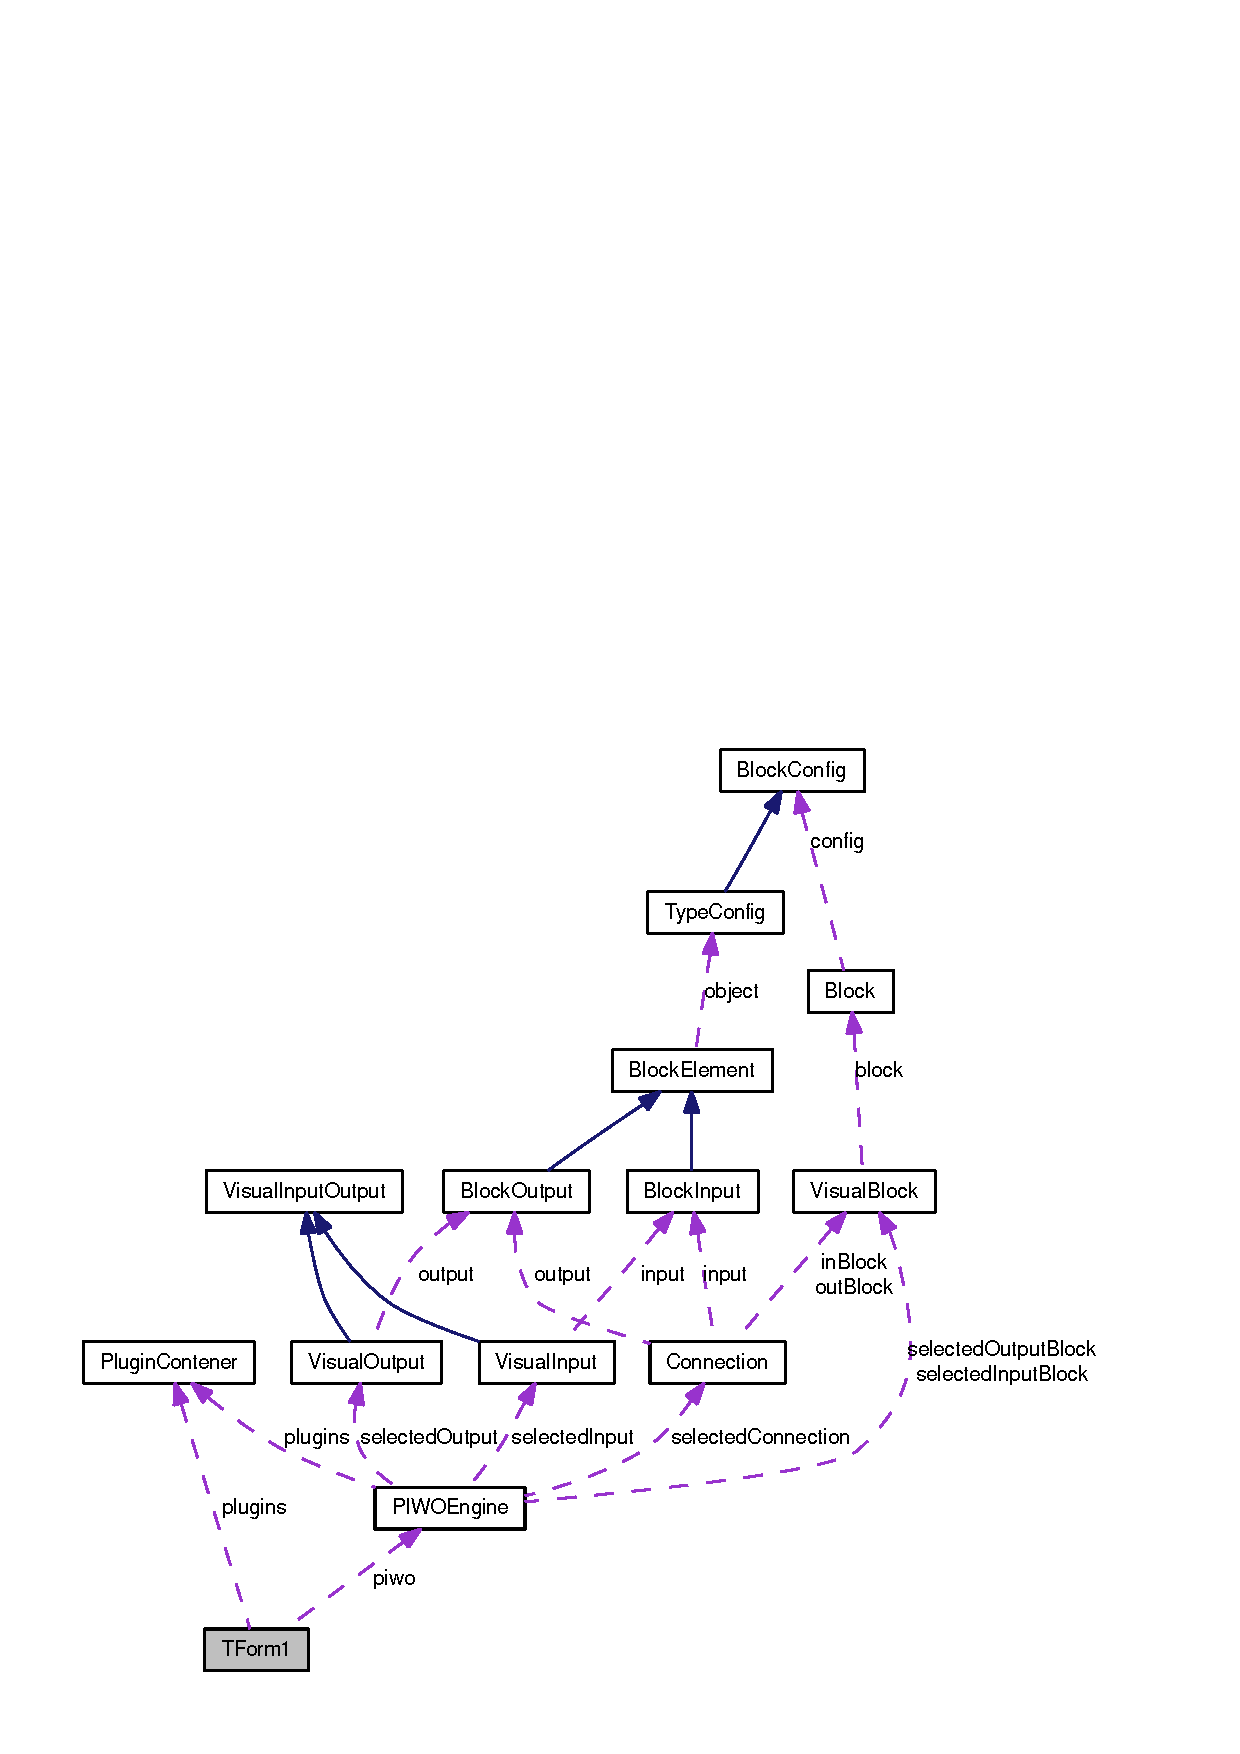
\includegraphics[width=400pt]{classTForm1__coll__graph}
\end{center}
\end{figure}
\subsection*{Public Member Functions}
\begin{CompactItemize}
\item 
void \_\-\_\-fastcall \hyperlink{classTForm1_b28b545fbae8b12c714f4ba8d664e831}{FormCreate} (TObject $\ast$Sender)
\item 
void \_\-\_\-fastcall \hyperlink{classTForm1_21263e28fe98f4d7da87b0f9fb411906}{Zakocz2Click} (TObject $\ast$Sender)
\item 
void \_\-\_\-fastcall \hyperlink{classTForm1_1ea3b1aff58b60bd5338bceb94416ea4}{Zaznaczwszystkiebloki1Click} (TObject $\ast$Sender)
\item 
void \_\-\_\-fastcall \hyperlink{classTForm1_8ddf63f3c72f524fb3e70559d2add67e}{Odznaczwszystkiebloki1Click} (TObject $\ast$Sender)
\item 
void \_\-\_\-fastcall \hyperlink{classTForm1_af1673c47adc3d228f6e6399c76a226d}{Odwrzaznaczenieblokw1Click} (TObject $\ast$Sender)
\item 
void \_\-\_\-fastcall \hyperlink{classTForm1_788905f80f093f21a927242521e0ba78}{Usubloki1Click} (TObject $\ast$Sender)
\item 
void \_\-\_\-fastcall \hyperlink{classTForm1_ec78283bc0f4991e6950955004b60a77}{Usuzaznaczonebloki1Click} (TObject $\ast$Sender)
\item 
void \_\-\_\-fastcall \hyperlink{classTForm1_4e73d3a0fa76a760e8c42b99cb7ca967}{Odznaczzaznaczonepoaczenie1Click} (TObject $\ast$Sender)
\item 
void \_\-\_\-fastcall \hyperlink{classTForm1_fabef0363a8b392dc9bee0438cf334d0}{Usuwszystkiepoczenia1Click} (TObject $\ast$Sender)
\item 
void \_\-\_\-fastcall \hyperlink{classTForm1_87e9a6d2f937b88c477d046b2852109f}{Usuzaznaczonepoczenie1Click} (TObject $\ast$Sender)
\item 
void \_\-\_\-fastcall \hyperlink{classTForm1_013f6ffc037839e3f5251728a89fb168}{Zresetujwszystkiepoczenia1Click} (TObject $\ast$Sender)
\item 
void \_\-\_\-fastcall \hyperlink{classTForm1_6f6d2f51dc3a2e41541c4df797536486}{Zresetujzaznaczonepoczenie1Click} (TObject $\ast$Sender)
\item 
void \_\-\_\-fastcall \hyperlink{classTForm1_979be199e4088eb73e1a199eb11531e0}{Uruchomwszystko1Click} (TObject $\ast$Sender)
\item 
void \_\-\_\-fastcall \hyperlink{classTForm1_12f0a6355c0fe7748f97378e8d83d0e2}{Uruchom3Click} (TObject $\ast$Sender)
\item 
void \_\-\_\-fastcall \hyperlink{classTForm1_327201e8ba2ffe5f8a866306f4ab602d}{PageControl1Resize} (TObject $\ast$Sender)
\item 
void \_\-\_\-fastcall \hyperlink{classTForm1_1c7229a551faa6b9095eb523b0843122}{Wyczylogi1Click} (TObject $\ast$Sender)
\item 
void \_\-\_\-fastcall \hyperlink{classTForm1_2f1df2a24662cbe737ae88633dbdcbc2}{MenuItem1Click} (TObject $\ast$Sender)
\item 
void \_\-\_\-fastcall \hyperlink{classTForm1_c43ab1208fdd1700242479091fa54bfa}{MenuItem3Click} (TObject $\ast$Sender)
\item 
void \_\-\_\-fastcall \hyperlink{classTForm1_aa65d93be5f8ead0aa96f29accddb0a8}{Zapiszdopliku1Zapiszjako1ClickClick} (TObject $\ast$Sender)
\item 
void \_\-\_\-fastcall \hyperlink{classTForm1_aa4a9501874d8b9736ef9c6ab19d93da}{MenuItem2Click} (TObject $\ast$Sender)
\item 
void \_\-\_\-fastcall \hyperlink{classTForm1_1c52133d24858202380937319bed525c}{MenuItem4Click} (TObject $\ast$Sender)
\item 
void \_\-\_\-fastcall \hyperlink{classTForm1_9830055131dd01fedd0c8212edec6a9b}{PageControl1Change} (TObject $\ast$Sender)
\item 
void \_\-\_\-fastcall \hyperlink{classTForm1_cfd8fc7d5e071f91d545cf71cd3e525c}{SpeedButton1Click} (TObject $\ast$Sender)
\item 
void \_\-\_\-fastcall \hyperlink{classTForm1_bc9c59c8c54a39ff8b9a8b1a8facdfde}{Timer1Timer} (TObject $\ast$Sender)
\item 
void \_\-\_\-fastcall \hyperlink{classTForm1_49836e6b4443972a738957868beb5894}{Nowy1Click} (TObject $\ast$Sender)
\item 
void \_\-\_\-fastcall \hyperlink{classTForm1_6ecd2685a5128166bd573ff3ebe1b37d}{Zakocz1Click} (TObject $\ast$Sender)
\item 
void \_\-\_\-fastcall \hyperlink{classTForm1_f63d66a27ca087cc5997b90fe1e2cec0}{Otwrz1Click} (TObject $\ast$Sender)
\item 
void \_\-\_\-fastcall \hyperlink{classTForm1_905eccb6be3dfda63ebceb962004286f}{Duplikujbloki1Click} (TObject $\ast$Sender)
\item 
void \_\-\_\-fastcall \hyperlink{classTForm1_f8d02d580dfa34c21232b663bac20e69}{Exportujjakoobraz1Click} (TObject $\ast$Sender)
\item 
void \_\-\_\-fastcall \hyperlink{classTForm1_892e5a861ee39447c901bda936774a66}{Zapiszjako1Click} (TObject $\ast$Sender)
\item 
void \_\-\_\-fastcall \hyperlink{classTForm1_f3fc2edfe6864f1204a491d88a160202}{FormCloseQuery} (TObject $\ast$Sender, bool \&CanClose)
\item 
void \_\-\_\-fastcall \hyperlink{classTForm1_285e94be246f0e0b2b04885d45ad5a77}{Sprawdprojekt1Click} (TObject $\ast$Sender)
\item 
void \_\-\_\-fastcall \hyperlink{classTForm1_0aebc36097cbddf910fe57cd0a2afa35}{Anuluj1Click} (TObject $\ast$Sender)
\item 
void \_\-\_\-fastcall \hyperlink{classTForm1_a171e9a7877c477410034b7e10ed9843}{ToolButton11Click} (TObject $\ast$Sender)
\item 
void \_\-\_\-fastcall \hyperlink{classTForm1_f9b33b7f20eeb63d7de3f5334db5e538}{ToolButton18Click} (TObject $\ast$Sender)
\item 
void \_\-\_\-fastcall \hyperlink{classTForm1_b8f8eeee515fd162462380c9a0eb450e}{ToolButton19Click} (TObject $\ast$Sender)
\item 
void \_\-\_\-fastcall \hyperlink{classTForm1_ed5b7aeb13679cc44c7fa9fd3f3a0eff}{ToolButton20Click} (TObject $\ast$Sender)
\item 
void \_\-\_\-fastcall \hyperlink{classTForm1_b91cedf9d878aadab926009fdd6880fe}{ToolButton21Click} (TObject $\ast$Sender)
\item 
void \_\-\_\-fastcall \hyperlink{classTForm1_378f04e87d819886bcb3e20aa47ab90a}{ToolButton22Click} (TObject $\ast$Sender)
\item 
void \_\-\_\-fastcall \hyperlink{classTForm1_f8af464cefaf41db4e61e56f3066638c}{FormDestroy} (TObject $\ast$Sender)
\item 
void \_\-\_\-fastcall \hyperlink{classTForm1_1c822362efe786992cc566620f2364ae}{Widok1Click} (TObject $\ast$Sender)
\item 
void \_\-\_\-fastcall \hyperlink{classTForm1_6fad014f2d10de311b9205f7aa47f93f}{Zamknijwszystkieokna1Click} (TObject $\ast$Sender)
\item 
void \_\-\_\-fastcall \hyperlink{classTForm1_f6a2b0b43deb2c48726155f268204529}{Pokawszystkieokna1Click} (TObject $\ast$Sender)
\item 
void \_\-\_\-fastcall \hyperlink{classTForm1_c392ee503212147cd1ad1b424ca75552}{Oprogramie1Click} (TObject $\ast$Sender)
\item 
void \_\-\_\-fastcall \hyperlink{classTForm1_5c7d023f63fa47e531de3634725067f6}{FormKeyDown} (TObject $\ast$Sender, WORD \&Key, TShiftState Shift)
\item 
void \_\-\_\-fastcall \hyperlink{classTForm1_057ec76bdcf16cf01e63de0fe0c7eab1}{ApplicationEvents1Message} (tagMSG \&Msg, bool \&Handled)
\item 
void \_\-\_\-fastcall \hyperlink{classTForm1_4ad666f572df484596275292dfff633a}{Instrukcjauytkoniwka1Click} (TObject $\ast$Sender)
\item 
void \_\-\_\-fastcall \hyperlink{classTForm1_8e6db4f096e5cf3cfc4db6f436d28831}{Dokumentacjatechniczna1Click} (TObject $\ast$Sender)
\item 
void \_\-\_\-fastcall \hyperlink{classTForm1_d6cdb94fa817f5076531e3bf29e4d9ab}{Oautorach1Click} (TObject $\ast$Sender)
\item 
void \hyperlink{classTForm1_579dfded9c383d2fd684e2405dc6371b}{addExt} (const AnsiString \&ExtMyFile)
\item 
\_\-\_\-fastcall \hyperlink{classTForm1_4b77eaf706e8386bc8d79ec547efc8b9}{TForm1} (TComponent $\ast$Owner)
\end{CompactItemize}
\subsection*{Public Attributes}
\begin{CompactItemize}
\item 
TMainMenu $\ast$ \hyperlink{classTForm1_fb129674fc9747697ab1ec4939462c70}{MainMenu1}
\item 
TMenuItem $\ast$ \hyperlink{classTForm1_bab442b2f1649d0026ddbaab2b772a94}{Plik1}
\item 
TMenuItem $\ast$ \hyperlink{classTForm1_380df144ba8d51b25de931a634bc6be2}{Edycja1}
\item 
TMenuItem $\ast$ \hyperlink{classTForm1_939bf0f4120695d5394e0cb2878683b2}{Nowy1}
\item 
TMenuItem $\ast$ \hyperlink{classTForm1_5186111e79ab009942940b48a0df9038}{Otwrz1}
\item 
TMenuItem $\ast$ \hyperlink{classTForm1_5fe7e2f7660a34d162b29f08e0542350}{Zapisz1}
\item 
TMenuItem $\ast$ \hyperlink{classTForm1_f4ce8bd1ea8a930a09853d724191f193}{Zapiszjako1}
\item 
TMenuItem $\ast$ \hyperlink{classTForm1_c8bedfca7b5dfed39edaff95ffb0577d}{Exportujjakoobraz1}
\item 
TMenuItem $\ast$ \hyperlink{classTForm1_6a033c3575a2e29c17d7c286029980f1}{Zakocz1}
\item 
TMenuItem $\ast$ \hyperlink{classTForm1_c11d4781566f19fd9dae9e3375ab1471}{Zaznaczwszystkiebloki1}
\item 
TMenuItem $\ast$ \hyperlink{classTForm1_81af1788cb8fedfe45c5ab1e9d6fa84f}{Odznaczwszystkiebloki1}
\item 
TMenuItem $\ast$ \hyperlink{classTForm1_55584a766db0eae448a1b827e95f9039}{Odwrzaznaczenieblokw1}
\item 
TMenuItem $\ast$ \hyperlink{classTForm1_fca8fb962a23fccc15b91c8770882a85}{Duplikujbloki1}
\item 
TMenuItem $\ast$ \hyperlink{classTForm1_67b6559358def61c012bd907a2994bdd}{Usubloki1}
\item 
TMenuItem $\ast$ \hyperlink{classTForm1_48a11274b861b0740194377fb412fc3c}{N1}
\item 
TMenuItem $\ast$ \hyperlink{classTForm1_b20e20b8aa20deb0db8782088a385b2f}{Zakocz2}
\item 
TMenuItem $\ast$ \hyperlink{classTForm1_655f428c436b429b7ca71c131bae8e35}{Usuzaznaczonebloki1}
\item 
TMenuItem $\ast$ \hyperlink{classTForm1_fb3981dd76bf7b054bed4b9ff9faab3f}{Odznaczzaznaczonepoaczenie1}
\item 
TMenuItem $\ast$ \hyperlink{classTForm1_725cf7f5e578ee304efeeb97522e4812}{Usuwszystkiepoczenia1}
\item 
TMenuItem $\ast$ \hyperlink{classTForm1_3a1a0d7e4b61af79e2119fc8e171b267}{Usuzaznaczonepoczenie1}
\item 
TMenuItem $\ast$ \hyperlink{classTForm1_1be67d689b1e4751c5043657cde7fb7e}{Pomoc1}
\item 
TMenuItem $\ast$ \hyperlink{classTForm1_015daea982a9bfc8c84724ed5db93435}{Instrukcjauytkoniwka1}
\item 
TMenuItem $\ast$ \hyperlink{classTForm1_edc7039427508f681377845a13eb7c5b}{Dokumentacjatechniczna1}
\item 
TMenuItem $\ast$ \hyperlink{classTForm1_bfdab287b3fce9e306b007b0530e90ac}{Oautorach1}
\item 
TMenuItem $\ast$ \hyperlink{classTForm1_9ed5ecf8b1efefab3f773cfbd4c163d9}{Oprogramie1}
\item 
TImageList $\ast$ \hyperlink{classTForm1_6eb05a9c9d980ca92fa5a9dd976116df}{ImageList1}
\item 
TStatusBar $\ast$ \hyperlink{classTForm1_ad39517b2c266c91d742acba97cec969}{StatusBar1}
\item 
TMenuItem $\ast$ \hyperlink{classTForm1_cc303ecddd253f90d5b943f96828b5ff}{Uruchom2}
\item 
TMenuItem $\ast$ \hyperlink{classTForm1_ab12b0763ade8d2303fc0d9e9dba2757}{Uruchomwszystko1}
\item 
TMenuItem $\ast$ \hyperlink{classTForm1_6f669f8e377edc9a83fc863c880a2940}{Uruchom3}
\item 
TMenuItem $\ast$ \hyperlink{classTForm1_82b4fa841135fca89c74efd1a699ba6d}{Zresetujwszystkiepoczenia1}
\item 
TMenuItem $\ast$ \hyperlink{classTForm1_a87f55c562f7b38bcf5e4388a94cf09c}{Zresetujzaznaczonepoczenie1}
\item 
TMenuItem $\ast$ \hyperlink{classTForm1_d022e2ac667384e64e28f323134fe641}{Widok1}
\item 
TPanel $\ast$ \hyperlink{classTForm1_42146ef4803abfd8ffd5d546f2465d6d}{Panel1}
\item 
TPageControl $\ast$ \hyperlink{classTForm1_0fc87f66d019c1324bc038c5beb168c0}{PageControl1}
\item 
TTabSheet $\ast$ \hyperlink{classTForm1_6d1c57fe4450ad878c2a4d8f65ffc72a}{TabSheet1}
\item 
TListView $\ast$ \hyperlink{classTForm1_10ab751cdcb401695d16b29bec7667da}{ListView1}
\item 
TTabSheet $\ast$ \hyperlink{classTForm1_bda9626de3a565ada75590e2a4072adb}{TabSheet2}
\item 
TTabSheet $\ast$ \hyperlink{classTForm1_9f711c2728656664dca851fae528647d}{TabSheet3}
\item 
TImageList $\ast$ \hyperlink{classTForm1_a1eb1de6f757fe4c219614eaa489d58c}{ImageList2}
\item 
TPopupMenu $\ast$ \hyperlink{classTForm1_2a7d717ee18c4392e29c02fb252d5edf}{PopupMenu1}
\item 
TMenuItem $\ast$ \hyperlink{classTForm1_9dcb2c2b046afeb5bd3d1e6110233ca1}{Wyczylogi1}
\item 
TMenuItem $\ast$ \hyperlink{classTForm1_9daa7303230ddb9903f9ed31489bf9bd}{Zapiszdopliku1}
\item 
TListView $\ast$ \hyperlink{classTForm1_f2bf95d7f40c9081bff58919fac42e27}{ListView2}
\item 
TListView $\ast$ \hyperlink{classTForm1_2ebb9796da3f2296c14d506af21d929e}{ListView3}
\item 
TSaveDialog $\ast$ \hyperlink{classTForm1_69479cd188c830cd26b871bc9d1bec6b}{SaveDialog1}
\item 
TPopupMenu $\ast$ \hyperlink{classTForm1_183d2be2116d1bd81ba3265063cd7862}{PopupMenu2}
\item 
TMenuItem $\ast$ \hyperlink{classTForm1_fa2b3db47d8e6084396230ca1faacae1}{MenuItem1}
\item 
TMenuItem $\ast$ \hyperlink{classTForm1_991d92316da7bc45269d39af1fd998e5}{MenuItem2}
\item 
TPopupMenu $\ast$ \hyperlink{classTForm1_8084e0041ff8d5eb21b5632b4caf5fff}{PopupMenu3}
\item 
TMenuItem $\ast$ \hyperlink{classTForm1_ef1f9c24509fa2b840942e0c522eaa49}{MenuItem3}
\item 
TMenuItem $\ast$ \hyperlink{classTForm1_1d34fca1a439e8d1b1899d0fd3734fa1}{MenuItem4}
\item 
TToolBar $\ast$ \hyperlink{classTForm1_0b61aacff668f8478628ce9fb2c7679f}{ToolBar1}
\item 
TPanel $\ast$ \hyperlink{classTForm1_1c581dd73461c34e5408cd163f026386}{Panel2}
\item 
TCGauge $\ast$ \hyperlink{classTForm1_3d74c84c60d687c60511fe44a7f04514}{CGauge1}
\item 
TLabel $\ast$ \hyperlink{classTForm1_c5a132daa716561ea42ea51c60c952e1}{Label1}
\item 
TSpeedButton $\ast$ \hyperlink{classTForm1_4910802fa9b4883b9e3991db1015c7ab}{SpeedButton1}
\item 
TTimer $\ast$ \hyperlink{classTForm1_b485ef6199745c5c2982d8368ec9d1ff}{Timer1}
\item 
TMenuItem $\ast$ \hyperlink{classTForm1_70c2a2eb6c9f1bd59047ef27a073e515}{Anuluj1}
\item 
TSaveDialog $\ast$ \hyperlink{classTForm1_144e0a54931b8c3fdfcaa6ffbccd4bb8}{SaveDialog2}
\item 
TOpenDialog $\ast$ \hyperlink{classTForm1_355801e3a8dc885ec19da6b9a5c3aecf}{OpenDialog1}
\item 
TToolButton $\ast$ \hyperlink{classTForm1_16b516ed8315336626ef543084163b91}{ToolButton1}
\item 
TToolButton $\ast$ \hyperlink{classTForm1_28ac629b0279cc5d013d72add3ed41ce}{ToolButton2}
\item 
TToolButton $\ast$ \hyperlink{classTForm1_bc287a73f306ead728aa949a32876c0d}{ToolButton3}
\item 
TToolButton $\ast$ \hyperlink{classTForm1_8d7c119ff7216835783eff16f3672135}{ToolButton4}
\item 
TToolButton $\ast$ \hyperlink{classTForm1_239ab7cfcbf5e165d1dd4c29d6d06542}{ToolButton5}
\item 
TToolButton $\ast$ \hyperlink{classTForm1_f716972f3abf585457033528a9c3f03c}{ToolButton6}
\item 
TToolButton $\ast$ \hyperlink{classTForm1_ece2f6432ce9ba88a0de83283c7621d3}{ToolButton7}
\item 
TToolButton $\ast$ \hyperlink{classTForm1_77d558c092eb5fc084d253e4da0a02c7}{ToolButton8}
\item 
TToolButton $\ast$ \hyperlink{classTForm1_dab7a30ee8cee50b2e417c4c1bc5ec47}{ToolButton9}
\item 
TToolButton $\ast$ \hyperlink{classTForm1_3b3935ddfee9e1d21980a15a4cff512c}{ToolButton10}
\item 
TToolButton $\ast$ \hyperlink{classTForm1_878606b0648b29677e804bf2e2814ddd}{ToolButton11}
\item 
TToolButton $\ast$ \hyperlink{classTForm1_165b84429874244e7adafd6a40d544fb}{ToolButton12}
\item 
TToolButton $\ast$ \hyperlink{classTForm1_abbbbef41138d1af9106b37203916115}{ToolButton13}
\item 
TToolButton $\ast$ \hyperlink{classTForm1_7f5544c0484108b05d7804d18e537032}{ToolButton14}
\item 
TToolButton $\ast$ \hyperlink{classTForm1_640f6c6b44c7b4e93f800ddf9415240d}{ToolButton15}
\item 
TToolButton $\ast$ \hyperlink{classTForm1_a6f360b14445883aedb8f6ad892dc27f}{ToolButton16}
\item 
TToolButton $\ast$ \hyperlink{classTForm1_6d324e1cf8b3d25388e8444bb17cca3f}{ToolButton17}
\item 
TToolButton $\ast$ \hyperlink{classTForm1_6459f873cefb4680462772e31df931c4}{ToolButton18}
\item 
TToolButton $\ast$ \hyperlink{classTForm1_88347ab66f85c36c884738d8ee5e58a3}{ToolButton19}
\item 
TToolButton $\ast$ \hyperlink{classTForm1_632d7a7fb1f58ef1eaa7f06813c1eb3d}{ToolButton20}
\item 
TToolButton $\ast$ \hyperlink{classTForm1_14ccc6f80b7fb70f80552b772075bcd9}{ToolButton21}
\item 
TToolButton $\ast$ \hyperlink{classTForm1_221d9932d360c903b3c14f26d7b3ae90}{ToolButton22}
\item 
TToolButton $\ast$ \hyperlink{classTForm1_040e77d5967da02a5aa3c462055f510d}{ToolButton23}
\item 
TToolButton $\ast$ \hyperlink{classTForm1_a2f6a2763d31ea472eb438aefc802161}{ToolButton24}
\item 
TToolButton $\ast$ \hyperlink{classTForm1_1346d2adf8108f59475e9b51746d1b5d}{ToolButton25}
\item 
TToolButton $\ast$ \hyperlink{classTForm1_de1f9eff17d771f91c82706d6aa801ff}{ToolButton26}
\item 
TImageList $\ast$ \hyperlink{classTForm1_7d80296d375fe1604de82f41c6317466}{ImageList3}
\item 
TToolButton $\ast$ \hyperlink{classTForm1_f25d192dc2f51425796a90e4aa58c987}{ToolButton27}
\item 
TMenuItem $\ast$ \hyperlink{classTForm1_70c28fd142eba444dc791df0eafc8385}{Sprawdprojekt1}
\item 
TBevel $\ast$ \hyperlink{classTForm1_fe711fe83a9246f1d158850214061ca4}{Bevel1}
\item 
TMenuItem $\ast$ \hyperlink{classTForm1_fbdc23537e25379aa4c73992641a843f}{Zamknijwszystkieokna1}
\item 
TMenuItem $\ast$ \hyperlink{classTForm1_7b4041d435033e2479bc5df13517e561}{Pokawszystkieokna1}
\item 
TMenuItem $\ast$ \hyperlink{classTForm1_7572e947da6f9d95c11b3ec671dbede4}{N2}
\item 
TApplicationEvents $\ast$ \hyperlink{classTForm1_85037aa8ea01d760f08123d791c416dd}{ApplicationEvents1}
\item 
\hyperlink{classPluginContener}{PluginContener} \hyperlink{classTForm1_d9cbc2c28df5c7941456e1333281ac43}{plugins}
\end{CompactItemize}
\subsection*{Private Member Functions}
\begin{CompactItemize}
\item 
void \hyperlink{classTForm1_4e07d96a5ae579b4ee90fa1b7744e7a2}{OnLoadProgress} (void $\ast$Sender, int position, int max, AnsiString info, int id)
\item 
void \hyperlink{classTForm1_9daceac11a528e49d52a5131e12aebe5}{OnFunctionAddClick} (void $\ast$Sender)
\item 
void \hyperlink{classTForm1_75b6c8accb0441ab6aaa5c6cc834bea0}{OnLogInformation} (TObject $\ast$Sender, const AnsiString message)
\item 
void \hyperlink{classTForm1_9673ad61a576d47d7ad53cb13a3e5a4d}{OnLogDebug} (TObject $\ast$Sender, const AnsiString message)
\item 
void \hyperlink{classTForm1_dfbe2953cac1319d0754474438b2d2b6}{OnLogWarrning} (TObject $\ast$Sender, const AnsiString message)
\item 
void \hyperlink{classTForm1_067a9fd8ad4f3b2a59c34f8e317cbbc7}{OnLogSuccess} (TObject $\ast$Sender, const AnsiString message)
\item 
void \hyperlink{classTForm1_080ddd93d3196c33b74c50c15b3720eb}{OnLogError} (TObject $\ast$Sender, const AnsiString message)
\item 
void \hyperlink{classTForm1_cf5d1f0fac58364f539deb0bd46c4c49}{OnLogRunInformation} (TObject $\ast$Sender, const AnsiString message)
\item 
void \hyperlink{classTForm1_62c5ecb809ce9a5473816fb013f4260e}{OnLogRunDebug} (TObject $\ast$Sender, const AnsiString message)
\item 
void \hyperlink{classTForm1_807c0c99b2bbeb91113b83131309cecc}{OnLogRunWarrning} (TObject $\ast$Sender, const AnsiString message)
\item 
void \hyperlink{classTForm1_9d4f79fae095cda30188324ad61a95a0}{OnLogRunSuccess} (TObject $\ast$Sender, const AnsiString message)
\item 
void \hyperlink{classTForm1_ffda0a341f5610795fb4815bc8e138ec}{OnLogRunError} (TObject $\ast$Sender, const AnsiString message)
\item 
void \hyperlink{classTForm1_7295024a0639ad522328b213cb06e821}{OnRunStart} (TObject $\ast$Sender)
\item 
void \hyperlink{classTForm1_c404db6653ee5eca5c04ae0fb9e8e5fd}{OnRunEnd} (TObject $\ast$Sender)
\item 
void \hyperlink{classTForm1_34173b9dc2ccd99660a6a602eec607a4}{OnRunProgress} (TObject $\ast$Sender, const AnsiString message, const double precent)
\item 
void \hyperlink{classTForm1_a7224379c3a100f708cf83e57d021b85}{OnChanged} (TObject $\ast$Sender)
\item 
void \hyperlink{classTForm1_ac255960d6054a626a606621787a7d0f}{OnBlockSelected} (TObject $\ast$Sender)
\item 
void \hyperlink{classTForm1_dcc5e70c6599d92da32b110ba459978c}{OnConnectionSelected} (TObject $\ast$Sender)
\item 
void \hyperlink{classTForm1_42c28a6bc0602d30253e83d138bb4964}{OnNothingSelected} (TObject $\ast$Sender)
\item 
void \_\-\_\-fastcall \hyperlink{classTForm1_dfa4ff1b700ae559e155a6383d28f1be}{HistoryMenuClick} (TObject $\ast$Sender)
\item 
void \hyperlink{classTForm1_7e8d6ef0115bb7fcb6cb5f7c3bf23890}{blockMenu} (bool blocked)
\item 
void \hyperlink{classTForm1_e3e2982ce4ac87941997bca9b06ec934}{newProject} ()
\item 
bool \hyperlink{classTForm1_2a46f5c794da332c1e9dd55ac0c03834}{closeProject} ()
\item 
void \hyperlink{classTForm1_a776111b5ba217e343c407bf9bebc00b}{openProject} ()
\end{CompactItemize}
\subsection*{Private Attributes}
\begin{CompactItemize}
\item 
\hyperlink{classPIWOEngine}{PIWOEngine} $\ast$ \hyperlink{classTForm1_b49ba3dff8624f56cb0374f140e6479d}{piwo}
\item 
AnsiString \hyperlink{classTForm1_654ca370064b6939024e2b18eab9d582}{fileName}
\item 
bool \hyperlink{classTForm1_308a6fe8b59a83de7a6a1dfbc49be29e}{isBlocked}
\item 
Graphics::TBitmap $\ast$ \hyperlink{classTForm1_0c8e62274e3d29dc58ed0a6b05637771}{defaultBlockImage}
\item 
vector$<$ \hyperlink{classFunctionDLL}{FunctionDLL} $\ast$ $>$ \hyperlink{classTForm1_dc19047fa18712f475ad00bd336c91d8}{top5Added}
\item 
vector$<$ TMenuItem $\ast$ $>$ \hyperlink{classTForm1_a61aac6247f2779f856ceeb1133e6ff3}{historyItems}
\item 
POINT \hyperlink{classTForm1_427dabcbbd77fff9d3354f2849333b44}{mousePos}
\end{CompactItemize}


\subsection{Detailed Description}


Definition at line 25 of file main.h.

\subsection{Constructor \& Destructor Documentation}
\hypertarget{classTForm1_4b77eaf706e8386bc8d79ec547efc8b9}{
\index{TForm1@{TForm1}!TForm1@{TForm1}}
\index{TForm1@{TForm1}!TForm1@{TForm1}}
\subsubsection[TForm1]{\setlength{\rightskip}{0pt plus 5cm}\_\-\_\-fastcall TForm1::TForm1 (TComponent $\ast$ {\em Owner})}}
\label{classTForm1_4b77eaf706e8386bc8d79ec547efc8b9}




Definition at line 19 of file main.cpp.

\subsection{Member Function Documentation}
\hypertarget{classTForm1_b28b545fbae8b12c714f4ba8d664e831}{
\index{TForm1@{TForm1}!FormCreate@{FormCreate}}
\index{FormCreate@{FormCreate}!TForm1@{TForm1}}
\subsubsection[FormCreate]{\setlength{\rightskip}{0pt plus 5cm}void \_\-\_\-fastcall TForm1::FormCreate (TObject $\ast$ {\em Sender})}}
\label{classTForm1_b28b545fbae8b12c714f4ba8d664e831}




Definition at line 107 of file main.cpp.

References addExt(), blockMenu(), CAPTION, PIWOEngine::defaultBlockImage, defaultBlockImage, fileName, Form2, ImageList1, PluginContener::LoadData(), PIWOEngine::loadFromFile(), TForm2::log, MainMenu1, newProject(), OnBlockSelected(), PIWOEngine::OnBlockSelected, OnChanged(), PIWOEngine::OnChanged, OnConnectionSelected(), PIWOEngine::OnConnectionSelected, PIWOEngine::OnDebug, PIWOEngine::OnError, OnFunctionAddClick(), PluginContener::OnFunctionAddRequest, PIWOEngine::OnInformation, PluginContener::OnLoadingProgress, OnLoadProgress(), OnLogDebug(), OnLogError(), OnLogInformation(), OnLogRunDebug(), OnLogRunError(), OnLogRunInformation(), OnLogRunSuccess(), OnLogRunWarrning(), OnLogSuccess(), OnLogWarrning(), OnNothingSelected(), PIWOEngine::OnNothingSelected, PIWOEngine::OnRunDebug, OnRunEnd(), PIWOEngine::OnRunEnd, PIWOEngine::OnRunError, PIWOEngine::OnRunInformation, OnRunProgress(), PIWOEngine::OnRunProgress, OnRunStart(), PIWOEngine::OnRunStart, PIWOEngine::OnRunSuccess, PIWOEngine::OnRunWarrning, PIWOEngine::OnSuccess, PIWOEngine::OnWarrning, OpenDialog1, PageControl1Change(), piwo, PIWOEngine::plugins, plugins, TForm2::ProgressBar1, and StatusBar1.\hypertarget{classTForm1_21263e28fe98f4d7da87b0f9fb411906}{
\index{TForm1@{TForm1}!Zakocz2Click@{Zakocz2Click}}
\index{Zakocz2Click@{Zakocz2Click}!TForm1@{TForm1}}
\subsubsection[Zakocz2Click]{\setlength{\rightskip}{0pt plus 5cm}void \_\-\_\-fastcall TForm1::Zakocz2Click (TObject $\ast$ {\em Sender})}}
\label{classTForm1_21263e28fe98f4d7da87b0f9fb411906}




Definition at line 400 of file main.cpp.\hypertarget{classTForm1_1ea3b1aff58b60bd5338bceb94416ea4}{
\index{TForm1@{TForm1}!Zaznaczwszystkiebloki1Click@{Zaznaczwszystkiebloki1Click}}
\index{Zaznaczwszystkiebloki1Click@{Zaznaczwszystkiebloki1Click}!TForm1@{TForm1}}
\subsubsection[Zaznaczwszystkiebloki1Click]{\setlength{\rightskip}{0pt plus 5cm}void \_\-\_\-fastcall TForm1::Zaznaczwszystkiebloki1Click (TObject $\ast$ {\em Sender})}}
\label{classTForm1_1ea3b1aff58b60bd5338bceb94416ea4}




Definition at line 406 of file main.cpp.

References piwo, and PIWOEngine::SelectAllBlocks().\hypertarget{classTForm1_8ddf63f3c72f524fb3e70559d2add67e}{
\index{TForm1@{TForm1}!Odznaczwszystkiebloki1Click@{Odznaczwszystkiebloki1Click}}
\index{Odznaczwszystkiebloki1Click@{Odznaczwszystkiebloki1Click}!TForm1@{TForm1}}
\subsubsection[Odznaczwszystkiebloki1Click]{\setlength{\rightskip}{0pt plus 5cm}void \_\-\_\-fastcall TForm1::Odznaczwszystkiebloki1Click (TObject $\ast$ {\em Sender})}}
\label{classTForm1_8ddf63f3c72f524fb3e70559d2add67e}




Definition at line 412 of file main.cpp.

References piwo, and PIWOEngine::UnselectAllBlocks().\hypertarget{classTForm1_af1673c47adc3d228f6e6399c76a226d}{
\index{TForm1@{TForm1}!Odwrzaznaczenieblokw1Click@{Odwrzaznaczenieblokw1Click}}
\index{Odwrzaznaczenieblokw1Click@{Odwrzaznaczenieblokw1Click}!TForm1@{TForm1}}
\subsubsection[Odwrzaznaczenieblokw1Click]{\setlength{\rightskip}{0pt plus 5cm}void \_\-\_\-fastcall TForm1::Odwrzaznaczenieblokw1Click (TObject $\ast$ {\em Sender})}}
\label{classTForm1_af1673c47adc3d228f6e6399c76a226d}




Definition at line 418 of file main.cpp.

References PIWOEngine::InvertBlockSelection(), and piwo.\hypertarget{classTForm1_788905f80f093f21a927242521e0ba78}{
\index{TForm1@{TForm1}!Usubloki1Click@{Usubloki1Click}}
\index{Usubloki1Click@{Usubloki1Click}!TForm1@{TForm1}}
\subsubsection[Usubloki1Click]{\setlength{\rightskip}{0pt plus 5cm}void \_\-\_\-fastcall TForm1::Usubloki1Click (TObject $\ast$ {\em Sender})}}
\label{classTForm1_788905f80f093f21a927242521e0ba78}




Definition at line 424 of file main.cpp.

References PIWOEngine::DeleteAllBlocks(), and piwo.\hypertarget{classTForm1_ec78283bc0f4991e6950955004b60a77}{
\index{TForm1@{TForm1}!Usuzaznaczonebloki1Click@{Usuzaznaczonebloki1Click}}
\index{Usuzaznaczonebloki1Click@{Usuzaznaczonebloki1Click}!TForm1@{TForm1}}
\subsubsection[Usuzaznaczonebloki1Click]{\setlength{\rightskip}{0pt plus 5cm}void \_\-\_\-fastcall TForm1::Usuzaznaczonebloki1Click (TObject $\ast$ {\em Sender})}}
\label{classTForm1_ec78283bc0f4991e6950955004b60a77}




Definition at line 430 of file main.cpp.

References PIWOEngine::DeleteSelectedBlocks(), PIWOEngine::DeleteSelectedConnection(), and piwo.\hypertarget{classTForm1_4e73d3a0fa76a760e8c42b99cb7ca967}{
\index{TForm1@{TForm1}!Odznaczzaznaczonepoaczenie1Click@{Odznaczzaznaczonepoaczenie1Click}}
\index{Odznaczzaznaczonepoaczenie1Click@{Odznaczzaznaczonepoaczenie1Click}!TForm1@{TForm1}}
\subsubsection[Odznaczzaznaczonepoaczenie1Click]{\setlength{\rightskip}{0pt plus 5cm}void \_\-\_\-fastcall TForm1::Odznaczzaznaczonepoaczenie1Click (TObject $\ast$ {\em Sender})}}
\label{classTForm1_4e73d3a0fa76a760e8c42b99cb7ca967}




Definition at line 437 of file main.cpp.

References piwo, and PIWOEngine::UnselectSelectedConnection().\hypertarget{classTForm1_fabef0363a8b392dc9bee0438cf334d0}{
\index{TForm1@{TForm1}!Usuwszystkiepoczenia1Click@{Usuwszystkiepoczenia1Click}}
\index{Usuwszystkiepoczenia1Click@{Usuwszystkiepoczenia1Click}!TForm1@{TForm1}}
\subsubsection[Usuwszystkiepoczenia1Click]{\setlength{\rightskip}{0pt plus 5cm}void \_\-\_\-fastcall TForm1::Usuwszystkiepoczenia1Click (TObject $\ast$ {\em Sender})}}
\label{classTForm1_fabef0363a8b392dc9bee0438cf334d0}




Definition at line 443 of file main.cpp.

References PIWOEngine::DeleteAllConnections(), and piwo.\hypertarget{classTForm1_87e9a6d2f937b88c477d046b2852109f}{
\index{TForm1@{TForm1}!Usuzaznaczonepoczenie1Click@{Usuzaznaczonepoczenie1Click}}
\index{Usuzaznaczonepoczenie1Click@{Usuzaznaczonepoczenie1Click}!TForm1@{TForm1}}
\subsubsection[Usuzaznaczonepoczenie1Click]{\setlength{\rightskip}{0pt plus 5cm}void \_\-\_\-fastcall TForm1::Usuzaznaczonepoczenie1Click (TObject $\ast$ {\em Sender})}}
\label{classTForm1_87e9a6d2f937b88c477d046b2852109f}




Definition at line 449 of file main.cpp.

References PIWOEngine::DeleteSelectedBlocks(), PIWOEngine::DeleteSelectedConnection(), and piwo.\hypertarget{classTForm1_013f6ffc037839e3f5251728a89fb168}{
\index{TForm1@{TForm1}!Zresetujwszystkiepoczenia1Click@{Zresetujwszystkiepoczenia1Click}}
\index{Zresetujwszystkiepoczenia1Click@{Zresetujwszystkiepoczenia1Click}!TForm1@{TForm1}}
\subsubsection[Zresetujwszystkiepoczenia1Click]{\setlength{\rightskip}{0pt plus 5cm}void \_\-\_\-fastcall TForm1::Zresetujwszystkiepoczenia1Click (TObject $\ast$ {\em Sender})}}
\label{classTForm1_013f6ffc037839e3f5251728a89fb168}




Definition at line 457 of file main.cpp.

References PIWOEngine::CancelCustomizationOnAllConnections(), and piwo.\hypertarget{classTForm1_6f6d2f51dc3a2e41541c4df797536486}{
\index{TForm1@{TForm1}!Zresetujzaznaczonepoczenie1Click@{Zresetujzaznaczonepoczenie1Click}}
\index{Zresetujzaznaczonepoczenie1Click@{Zresetujzaznaczonepoczenie1Click}!TForm1@{TForm1}}
\subsubsection[Zresetujzaznaczonepoczenie1Click]{\setlength{\rightskip}{0pt plus 5cm}void \_\-\_\-fastcall TForm1::Zresetujzaznaczonepoczenie1Click (TObject $\ast$ {\em Sender})}}
\label{classTForm1_6f6d2f51dc3a2e41541c4df797536486}




Definition at line 463 of file main.cpp.

References PIWOEngine::CancelCustomizationOnSelectedConnections(), and piwo.\hypertarget{classTForm1_979be199e4088eb73e1a199eb11531e0}{
\index{TForm1@{TForm1}!Uruchomwszystko1Click@{Uruchomwszystko1Click}}
\index{Uruchomwszystko1Click@{Uruchomwszystko1Click}!TForm1@{TForm1}}
\subsubsection[Uruchomwszystko1Click]{\setlength{\rightskip}{0pt plus 5cm}void \_\-\_\-fastcall TForm1::Uruchomwszystko1Click (TObject $\ast$ {\em Sender})}}
\label{classTForm1_979be199e4088eb73e1a199eb11531e0}




Definition at line 469 of file main.cpp.

References blockMenu(), piwo, and PIWOEngine::run().\hypertarget{classTForm1_12f0a6355c0fe7748f97378e8d83d0e2}{
\index{TForm1@{TForm1}!Uruchom3Click@{Uruchom3Click}}
\index{Uruchom3Click@{Uruchom3Click}!TForm1@{TForm1}}
\subsubsection[Uruchom3Click]{\setlength{\rightskip}{0pt plus 5cm}void \_\-\_\-fastcall TForm1::Uruchom3Click (TObject $\ast$ {\em Sender})}}
\label{classTForm1_12f0a6355c0fe7748f97378e8d83d0e2}




Definition at line 477 of file main.cpp.

References PIWOEngine::alwaysRun, piwo, PIWOEngine::run(), ToolButton14, and Uruchom3.\hypertarget{classTForm1_327201e8ba2ffe5f8a866306f4ab602d}{
\index{TForm1@{TForm1}!PageControl1Resize@{PageControl1Resize}}
\index{PageControl1Resize@{PageControl1Resize}!TForm1@{TForm1}}
\subsubsection[PageControl1Resize]{\setlength{\rightskip}{0pt plus 5cm}void \_\-\_\-fastcall TForm1::PageControl1Resize (TObject $\ast$ {\em Sender})}}
\label{classTForm1_327201e8ba2ffe5f8a866306f4ab602d}




Definition at line 487 of file main.cpp.

References Label1, ListView1, ListView2, ListView3, PageControl1, TabSheet1, TabSheet2, and TabSheet3.

Referenced by OnLogDebug(), OnLogError(), OnLogInformation(), OnLogRunDebug(), OnLogRunError(), OnLogRunInformation(), OnLogRunSuccess(), OnLogRunWarrning(), OnLogSuccess(), OnLogWarrning(), and PageControl1Change().\hypertarget{classTForm1_1c7229a551faa6b9095eb523b0843122}{
\index{TForm1@{TForm1}!Wyczylogi1Click@{Wyczylogi1Click}}
\index{Wyczylogi1Click@{Wyczylogi1Click}!TForm1@{TForm1}}
\subsubsection[Wyczylogi1Click]{\setlength{\rightskip}{0pt plus 5cm}void \_\-\_\-fastcall TForm1::Wyczylogi1Click (TObject $\ast$ {\em Sender})}}
\label{classTForm1_1c7229a551faa6b9095eb523b0843122}




Definition at line 497 of file main.cpp.

References ListView1.\hypertarget{classTForm1_2f1df2a24662cbe737ae88633dbdcbc2}{
\index{TForm1@{TForm1}!MenuItem1Click@{MenuItem1Click}}
\index{MenuItem1Click@{MenuItem1Click}!TForm1@{TForm1}}
\subsubsection[MenuItem1Click]{\setlength{\rightskip}{0pt plus 5cm}void \_\-\_\-fastcall TForm1::MenuItem1Click (TObject $\ast$ {\em Sender})}}
\label{classTForm1_2f1df2a24662cbe737ae88633dbdcbc2}




Definition at line 503 of file main.cpp.

References ListView2.\hypertarget{classTForm1_c43ab1208fdd1700242479091fa54bfa}{
\index{TForm1@{TForm1}!MenuItem3Click@{MenuItem3Click}}
\index{MenuItem3Click@{MenuItem3Click}!TForm1@{TForm1}}
\subsubsection[MenuItem3Click]{\setlength{\rightskip}{0pt plus 5cm}void \_\-\_\-fastcall TForm1::MenuItem3Click (TObject $\ast$ {\em Sender})}}
\label{classTForm1_c43ab1208fdd1700242479091fa54bfa}




Definition at line 509 of file main.cpp.

References ListView3.\hypertarget{classTForm1_aa65d93be5f8ead0aa96f29accddb0a8}{
\index{TForm1@{TForm1}!Zapiszdopliku1Zapiszjako1ClickClick@{Zapiszdopliku1Zapiszjako1ClickClick}}
\index{Zapiszdopliku1Zapiszjako1ClickClick@{Zapiszdopliku1Zapiszjako1ClickClick}!TForm1@{TForm1}}
\subsubsection[Zapiszdopliku1Zapiszjako1ClickClick]{\setlength{\rightskip}{0pt plus 5cm}void \_\-\_\-fastcall TForm1::Zapiszdopliku1Zapiszjako1ClickClick (TObject $\ast$ {\em Sender})}}
\label{classTForm1_aa65d93be5f8ead0aa96f29accddb0a8}




Definition at line 515 of file main.cpp.

References ListView1, and SaveDialog1.\hypertarget{classTForm1_aa4a9501874d8b9736ef9c6ab19d93da}{
\index{TForm1@{TForm1}!MenuItem2Click@{MenuItem2Click}}
\index{MenuItem2Click@{MenuItem2Click}!TForm1@{TForm1}}
\subsubsection[MenuItem2Click]{\setlength{\rightskip}{0pt plus 5cm}void \_\-\_\-fastcall TForm1::MenuItem2Click (TObject $\ast$ {\em Sender})}}
\label{classTForm1_aa4a9501874d8b9736ef9c6ab19d93da}




Definition at line 541 of file main.cpp.

References ListView2, and SaveDialog1.\hypertarget{classTForm1_1c52133d24858202380937319bed525c}{
\index{TForm1@{TForm1}!MenuItem4Click@{MenuItem4Click}}
\index{MenuItem4Click@{MenuItem4Click}!TForm1@{TForm1}}
\subsubsection[MenuItem4Click]{\setlength{\rightskip}{0pt plus 5cm}void \_\-\_\-fastcall TForm1::MenuItem4Click (TObject $\ast$ {\em Sender})}}
\label{classTForm1_1c52133d24858202380937319bed525c}




Definition at line 567 of file main.cpp.

References ListView3, and SaveDialog1.\hypertarget{classTForm1_9830055131dd01fedd0c8212edec6a9b}{
\index{TForm1@{TForm1}!PageControl1Change@{PageControl1Change}}
\index{PageControl1Change@{PageControl1Change}!TForm1@{TForm1}}
\subsubsection[PageControl1Change]{\setlength{\rightskip}{0pt plus 5cm}void \_\-\_\-fastcall TForm1::PageControl1Change (TObject $\ast$ {\em Sender})}}
\label{classTForm1_9830055131dd01fedd0c8212edec6a9b}




Definition at line 594 of file main.cpp.

References ListView1, ListView2, ListView3, and PageControl1Resize().

Referenced by FormCreate().\hypertarget{classTForm1_cfd8fc7d5e071f91d545cf71cd3e525c}{
\index{TForm1@{TForm1}!SpeedButton1Click@{SpeedButton1Click}}
\index{SpeedButton1Click@{SpeedButton1Click}!TForm1@{TForm1}}
\subsubsection[SpeedButton1Click]{\setlength{\rightskip}{0pt plus 5cm}void \_\-\_\-fastcall TForm1::SpeedButton1Click (TObject $\ast$ {\em Sender})}}
\label{classTForm1_cfd8fc7d5e071f91d545cf71cd3e525c}




Definition at line 629 of file main.cpp.

References PIWOEngine::abort(), and piwo.\hypertarget{classTForm1_bc9c59c8c54a39ff8b9a8b1a8facdfde}{
\index{TForm1@{TForm1}!Timer1Timer@{Timer1Timer}}
\index{Timer1Timer@{Timer1Timer}!TForm1@{TForm1}}
\subsubsection[Timer1Timer]{\setlength{\rightskip}{0pt plus 5cm}void \_\-\_\-fastcall TForm1::Timer1Timer (TObject $\ast$ {\em Sender})}}
\label{classTForm1_bc9c59c8c54a39ff8b9a8b1a8facdfde}




Definition at line 638 of file main.cpp.

References Panel2, and Timer1.\hypertarget{classTForm1_49836e6b4443972a738957868beb5894}{
\index{TForm1@{TForm1}!Nowy1Click@{Nowy1Click}}
\index{Nowy1Click@{Nowy1Click}!TForm1@{TForm1}}
\subsubsection[Nowy1Click]{\setlength{\rightskip}{0pt plus 5cm}void \_\-\_\-fastcall TForm1::Nowy1Click (TObject $\ast$ {\em Sender})}}
\label{classTForm1_49836e6b4443972a738957868beb5894}




Definition at line 873 of file main.cpp.

References newProject().\hypertarget{classTForm1_6ecd2685a5128166bd573ff3ebe1b37d}{
\index{TForm1@{TForm1}!Zakocz1Click@{Zakocz1Click}}
\index{Zakocz1Click@{Zakocz1Click}!TForm1@{TForm1}}
\subsubsection[Zakocz1Click]{\setlength{\rightskip}{0pt plus 5cm}void \_\-\_\-fastcall TForm1::Zakocz1Click (TObject $\ast$ {\em Sender})}}
\label{classTForm1_6ecd2685a5128166bd573ff3ebe1b37d}




Definition at line 879 of file main.cpp.

References closeProject().\hypertarget{classTForm1_f63d66a27ca087cc5997b90fe1e2cec0}{
\index{TForm1@{TForm1}!Otwrz1Click@{Otwrz1Click}}
\index{Otwrz1Click@{Otwrz1Click}!TForm1@{TForm1}}
\subsubsection[Otwrz1Click]{\setlength{\rightskip}{0pt plus 5cm}void \_\-\_\-fastcall TForm1::Otwrz1Click (TObject $\ast$ {\em Sender})}}
\label{classTForm1_f63d66a27ca087cc5997b90fe1e2cec0}




Definition at line 885 of file main.cpp.

References openProject().\hypertarget{classTForm1_905eccb6be3dfda63ebceb962004286f}{
\index{TForm1@{TForm1}!Duplikujbloki1Click@{Duplikujbloki1Click}}
\index{Duplikujbloki1Click@{Duplikujbloki1Click}!TForm1@{TForm1}}
\subsubsection[Duplikujbloki1Click]{\setlength{\rightskip}{0pt plus 5cm}void \_\-\_\-fastcall TForm1::Duplikujbloki1Click (TObject $\ast$ {\em Sender})}}
\label{classTForm1_905eccb6be3dfda63ebceb962004286f}




Definition at line 891 of file main.cpp.

References PIWOEngine::DuplcateSelectedBlocks(), and piwo.\hypertarget{classTForm1_f8d02d580dfa34c21232b663bac20e69}{
\index{TForm1@{TForm1}!Exportujjakoobraz1Click@{Exportujjakoobraz1Click}}
\index{Exportujjakoobraz1Click@{Exportujjakoobraz1Click}!TForm1@{TForm1}}
\subsubsection[Exportujjakoobraz1Click]{\setlength{\rightskip}{0pt plus 5cm}void \_\-\_\-fastcall TForm1::Exportujjakoobraz1Click (TObject $\ast$ {\em Sender})}}
\label{classTForm1_f8d02d580dfa34c21232b663bac20e69}




Definition at line 897 of file main.cpp.

References CAPTION, fileName, piwo, SaveDialog2, PIWOEngine::saveToFile(), and StatusBar1.

Referenced by Zapiszjako1Click().\hypertarget{classTForm1_892e5a861ee39447c901bda936774a66}{
\index{TForm1@{TForm1}!Zapiszjako1Click@{Zapiszjako1Click}}
\index{Zapiszjako1Click@{Zapiszjako1Click}!TForm1@{TForm1}}
\subsubsection[Zapiszjako1Click]{\setlength{\rightskip}{0pt plus 5cm}void \_\-\_\-fastcall TForm1::Zapiszjako1Click (TObject $\ast$ {\em Sender})}}
\label{classTForm1_892e5a861ee39447c901bda936774a66}




Definition at line 917 of file main.cpp.

References Exportujjakoobraz1Click(), fileName, piwo, and PIWOEngine::saveToFile().\hypertarget{classTForm1_f3fc2edfe6864f1204a491d88a160202}{
\index{TForm1@{TForm1}!FormCloseQuery@{FormCloseQuery}}
\index{FormCloseQuery@{FormCloseQuery}!TForm1@{TForm1}}
\subsubsection[FormCloseQuery]{\setlength{\rightskip}{0pt plus 5cm}void \_\-\_\-fastcall TForm1::FormCloseQuery (TObject $\ast$ {\em Sender}, \/  bool \& {\em CanClose})}}
\label{classTForm1_f3fc2edfe6864f1204a491d88a160202}




Definition at line 932 of file main.cpp.

References closeProject().\hypertarget{classTForm1_285e94be246f0e0b2b04885d45ad5a77}{
\index{TForm1@{TForm1}!Sprawdprojekt1Click@{Sprawdprojekt1Click}}
\index{Sprawdprojekt1Click@{Sprawdprojekt1Click}!TForm1@{TForm1}}
\subsubsection[Sprawdprojekt1Click]{\setlength{\rightskip}{0pt plus 5cm}void \_\-\_\-fastcall TForm1::Sprawdprojekt1Click (TObject $\ast$ {\em Sender})}}
\label{classTForm1_285e94be246f0e0b2b04885d45ad5a77}




Definition at line 985 of file main.cpp.

References piwo, and PIWOEngine::validateAll().\hypertarget{classTForm1_0aebc36097cbddf910fe57cd0a2afa35}{
\index{TForm1@{TForm1}!Anuluj1Click@{Anuluj1Click}}
\index{Anuluj1Click@{Anuluj1Click}!TForm1@{TForm1}}
\subsubsection[Anuluj1Click]{\setlength{\rightskip}{0pt plus 5cm}void \_\-\_\-fastcall TForm1::Anuluj1Click (TObject $\ast$ {\em Sender})}}
\label{classTForm1_0aebc36097cbddf910fe57cd0a2afa35}




Definition at line 991 of file main.cpp.

References PIWOEngine::abort(), and piwo.\hypertarget{classTForm1_a171e9a7877c477410034b7e10ed9843}{
\index{TForm1@{TForm1}!ToolButton11Click@{ToolButton11Click}}
\index{ToolButton11Click@{ToolButton11Click}!TForm1@{TForm1}}
\subsubsection[ToolButton11Click]{\setlength{\rightskip}{0pt plus 5cm}void \_\-\_\-fastcall TForm1::ToolButton11Click (TObject $\ast$ {\em Sender})}}
\label{classTForm1_a171e9a7877c477410034b7e10ed9843}




Definition at line 997 of file main.cpp.

References PIWOEngine::DeleteSelectedBlocks(), PIWOEngine::DeleteSelectedConnection(), and piwo.\hypertarget{classTForm1_f9b33b7f20eeb63d7de3f5334db5e538}{
\index{TForm1@{TForm1}!ToolButton18Click@{ToolButton18Click}}
\index{ToolButton18Click@{ToolButton18Click}!TForm1@{TForm1}}
\subsubsection[ToolButton18Click]{\setlength{\rightskip}{0pt plus 5cm}void \_\-\_\-fastcall TForm1::ToolButton18Click (TObject $\ast$ {\em Sender})}}
\label{classTForm1_f9b33b7f20eeb63d7de3f5334db5e538}




Definition at line 1018 of file main.cpp.

References OnFunctionAddClick(), and top5Added.\hypertarget{classTForm1_b8f8eeee515fd162462380c9a0eb450e}{
\index{TForm1@{TForm1}!ToolButton19Click@{ToolButton19Click}}
\index{ToolButton19Click@{ToolButton19Click}!TForm1@{TForm1}}
\subsubsection[ToolButton19Click]{\setlength{\rightskip}{0pt plus 5cm}void \_\-\_\-fastcall TForm1::ToolButton19Click (TObject $\ast$ {\em Sender})}}
\label{classTForm1_b8f8eeee515fd162462380c9a0eb450e}




Definition at line 1026 of file main.cpp.

References OnFunctionAddClick(), and top5Added.\hypertarget{classTForm1_ed5b7aeb13679cc44c7fa9fd3f3a0eff}{
\index{TForm1@{TForm1}!ToolButton20Click@{ToolButton20Click}}
\index{ToolButton20Click@{ToolButton20Click}!TForm1@{TForm1}}
\subsubsection[ToolButton20Click]{\setlength{\rightskip}{0pt plus 5cm}void \_\-\_\-fastcall TForm1::ToolButton20Click (TObject $\ast$ {\em Sender})}}
\label{classTForm1_ed5b7aeb13679cc44c7fa9fd3f3a0eff}




Definition at line 1034 of file main.cpp.

References OnFunctionAddClick(), and top5Added.\hypertarget{classTForm1_b91cedf9d878aadab926009fdd6880fe}{
\index{TForm1@{TForm1}!ToolButton21Click@{ToolButton21Click}}
\index{ToolButton21Click@{ToolButton21Click}!TForm1@{TForm1}}
\subsubsection[ToolButton21Click]{\setlength{\rightskip}{0pt plus 5cm}void \_\-\_\-fastcall TForm1::ToolButton21Click (TObject $\ast$ {\em Sender})}}
\label{classTForm1_b91cedf9d878aadab926009fdd6880fe}




Definition at line 1042 of file main.cpp.

References OnFunctionAddClick(), and top5Added.\hypertarget{classTForm1_378f04e87d819886bcb3e20aa47ab90a}{
\index{TForm1@{TForm1}!ToolButton22Click@{ToolButton22Click}}
\index{ToolButton22Click@{ToolButton22Click}!TForm1@{TForm1}}
\subsubsection[ToolButton22Click]{\setlength{\rightskip}{0pt plus 5cm}void \_\-\_\-fastcall TForm1::ToolButton22Click (TObject $\ast$ {\em Sender})}}
\label{classTForm1_378f04e87d819886bcb3e20aa47ab90a}




Definition at line 1050 of file main.cpp.

References OnFunctionAddClick(), and top5Added.\hypertarget{classTForm1_f8af464cefaf41db4e61e56f3066638c}{
\index{TForm1@{TForm1}!FormDestroy@{FormDestroy}}
\index{FormDestroy@{FormDestroy}!TForm1@{TForm1}}
\subsubsection[FormDestroy]{\setlength{\rightskip}{0pt plus 5cm}void \_\-\_\-fastcall TForm1::FormDestroy (TObject $\ast$ {\em Sender})}}
\label{classTForm1_f8af464cefaf41db4e61e56f3066638c}




Definition at line 1058 of file main.cpp.

References defaultBlockImage.\hypertarget{classTForm1_1c822362efe786992cc566620f2364ae}{
\index{TForm1@{TForm1}!Widok1Click@{Widok1Click}}
\index{Widok1Click@{Widok1Click}!TForm1@{TForm1}}
\subsubsection[Widok1Click]{\setlength{\rightskip}{0pt plus 5cm}void \_\-\_\-fastcall TForm1::Widok1Click (TObject $\ast$ {\em Sender})}}
\label{classTForm1_1c822362efe786992cc566620f2364ae}




Definition at line 1064 of file main.cpp.

References blockMenu(), historyItems, HistoryMenuClick(), PIWOEngine::historyWindows, isBlocked, MainMenu1, piwo, and Widok1.\hypertarget{classTForm1_6fad014f2d10de311b9205f7aa47f93f}{
\index{TForm1@{TForm1}!Zamknijwszystkieokna1Click@{Zamknijwszystkieokna1Click}}
\index{Zamknijwszystkieokna1Click@{Zamknijwszystkieokna1Click}!TForm1@{TForm1}}
\subsubsection[Zamknijwszystkieokna1Click]{\setlength{\rightskip}{0pt plus 5cm}void \_\-\_\-fastcall TForm1::Zamknijwszystkieokna1Click (TObject $\ast$ {\em Sender})}}
\label{classTForm1_6fad014f2d10de311b9205f7aa47f93f}




Definition at line 1109 of file main.cpp.

References PIWOEngine::historyWindows, and piwo.\hypertarget{classTForm1_f6a2b0b43deb2c48726155f268204529}{
\index{TForm1@{TForm1}!Pokawszystkieokna1Click@{Pokawszystkieokna1Click}}
\index{Pokawszystkieokna1Click@{Pokawszystkieokna1Click}!TForm1@{TForm1}}
\subsubsection[Pokawszystkieokna1Click]{\setlength{\rightskip}{0pt plus 5cm}void \_\-\_\-fastcall TForm1::Pokawszystkieokna1Click (TObject $\ast$ {\em Sender})}}
\label{classTForm1_f6a2b0b43deb2c48726155f268204529}




Definition at line 1120 of file main.cpp.

References PIWOEngine::historyWindows, and piwo.\hypertarget{classTForm1_c392ee503212147cd1ad1b424ca75552}{
\index{TForm1@{TForm1}!Oprogramie1Click@{Oprogramie1Click}}
\index{Oprogramie1Click@{Oprogramie1Click}!TForm1@{TForm1}}
\subsubsection[Oprogramie1Click]{\setlength{\rightskip}{0pt plus 5cm}void \_\-\_\-fastcall TForm1::Oprogramie1Click (TObject $\ast$ {\em Sender})}}
\label{classTForm1_c392ee503212147cd1ad1b424ca75552}




Definition at line 1131 of file main.cpp.

References Form4.\hypertarget{classTForm1_5c7d023f63fa47e531de3634725067f6}{
\index{TForm1@{TForm1}!FormKeyDown@{FormKeyDown}}
\index{FormKeyDown@{FormKeyDown}!TForm1@{TForm1}}
\subsubsection[FormKeyDown]{\setlength{\rightskip}{0pt plus 5cm}void \_\-\_\-fastcall TForm1::FormKeyDown (TObject $\ast$ {\em Sender}, \/  WORD \& {\em Key}, \/  TShiftState {\em Shift})}}
\label{classTForm1_5c7d023f63fa47e531de3634725067f6}




Definition at line 1140 of file main.cpp.

References PIWOEngine::DeleteSelectedBlocks(), PIWOEngine::DeleteSelectedConnection(), and piwo.\hypertarget{classTForm1_057ec76bdcf16cf01e63de0fe0c7eab1}{
\index{TForm1@{TForm1}!ApplicationEvents1Message@{ApplicationEvents1Message}}
\index{ApplicationEvents1Message@{ApplicationEvents1Message}!TForm1@{TForm1}}
\subsubsection[ApplicationEvents1Message]{\setlength{\rightskip}{0pt plus 5cm}void \_\-\_\-fastcall TForm1::ApplicationEvents1Message (tagMSG \& {\em Msg}, \/  bool \& {\em Handled})}}
\label{classTForm1_057ec76bdcf16cf01e63de0fe0c7eab1}




Definition at line 1152 of file main.cpp.

References mousePos.\hypertarget{classTForm1_4ad666f572df484596275292dfff633a}{
\index{TForm1@{TForm1}!Instrukcjauytkoniwka1Click@{Instrukcjauytkoniwka1Click}}
\index{Instrukcjauytkoniwka1Click@{Instrukcjauytkoniwka1Click}!TForm1@{TForm1}}
\subsubsection[Instrukcjauytkoniwka1Click]{\setlength{\rightskip}{0pt plus 5cm}void \_\-\_\-fastcall TForm1::Instrukcjauytkoniwka1Click (TObject $\ast$ {\em Sender})}}
\label{classTForm1_4ad666f572df484596275292dfff633a}




Definition at line 1164 of file main.cpp.\hypertarget{classTForm1_8e6db4f096e5cf3cfc4db6f436d28831}{
\index{TForm1@{TForm1}!Dokumentacjatechniczna1Click@{Dokumentacjatechniczna1Click}}
\index{Dokumentacjatechniczna1Click@{Dokumentacjatechniczna1Click}!TForm1@{TForm1}}
\subsubsection[Dokumentacjatechniczna1Click]{\setlength{\rightskip}{0pt plus 5cm}void \_\-\_\-fastcall TForm1::Dokumentacjatechniczna1Click (TObject $\ast$ {\em Sender})}}
\label{classTForm1_8e6db4f096e5cf3cfc4db6f436d28831}




Definition at line 1171 of file main.cpp.\hypertarget{classTForm1_d6cdb94fa817f5076531e3bf29e4d9ab}{
\index{TForm1@{TForm1}!Oautorach1Click@{Oautorach1Click}}
\index{Oautorach1Click@{Oautorach1Click}!TForm1@{TForm1}}
\subsubsection[Oautorach1Click]{\setlength{\rightskip}{0pt plus 5cm}void \_\-\_\-fastcall TForm1::Oautorach1Click (TObject $\ast$ {\em Sender})}}
\label{classTForm1_d6cdb94fa817f5076531e3bf29e4d9ab}




Definition at line 1178 of file main.cpp.

References Form5.\hypertarget{classTForm1_4e07d96a5ae579b4ee90fa1b7744e7a2}{
\index{TForm1@{TForm1}!OnLoadProgress@{OnLoadProgress}}
\index{OnLoadProgress@{OnLoadProgress}!TForm1@{TForm1}}
\subsubsection[OnLoadProgress]{\setlength{\rightskip}{0pt plus 5cm}void TForm1::OnLoadProgress (void $\ast$ {\em Sender}, \/  int {\em position}, \/  int {\em max}, \/  AnsiString {\em info}, \/  int {\em id})\hspace{0.3cm}{\tt  \mbox{[}private\mbox{]}}}}
\label{classTForm1_4e07d96a5ae579b4ee90fa1b7744e7a2}




Definition at line 24 of file main.cpp.

References Form2, TForm2::log, OnLogSuccess(), OnLogWarrning(), and TForm2::ProgressBar1.

Referenced by FormCreate().\hypertarget{classTForm1_9daceac11a528e49d52a5131e12aebe5}{
\index{TForm1@{TForm1}!OnFunctionAddClick@{OnFunctionAddClick}}
\index{OnFunctionAddClick@{OnFunctionAddClick}!TForm1@{TForm1}}
\subsubsection[OnFunctionAddClick]{\setlength{\rightskip}{0pt plus 5cm}void TForm1::OnFunctionAddClick (void $\ast$ {\em Sender})\hspace{0.3cm}{\tt  \mbox{[}private\mbox{]}}}}
\label{classTForm1_9daceac11a528e49d52a5131e12aebe5}




Definition at line 47 of file main.cpp.

References PIWOEngine::AddBlock(), ImageList3, FunctionDLL::name, piwo, and top5Added.

Referenced by FormCreate(), ToolButton18Click(), ToolButton19Click(), ToolButton20Click(), ToolButton21Click(), and ToolButton22Click().\hypertarget{classTForm1_75b6c8accb0441ab6aaa5c6cc834bea0}{
\index{TForm1@{TForm1}!OnLogInformation@{OnLogInformation}}
\index{OnLogInformation@{OnLogInformation}!TForm1@{TForm1}}
\subsubsection[OnLogInformation]{\setlength{\rightskip}{0pt plus 5cm}void TForm1::OnLogInformation (TObject $\ast$ {\em Sender}, \/  const AnsiString {\em message})\hspace{0.3cm}{\tt  \mbox{[}private\mbox{]}}}}
\label{classTForm1_75b6c8accb0441ab6aaa5c6cc834bea0}




Definition at line 198 of file main.cpp.

References ListView1, ListView3, and PageControl1Resize().

Referenced by FormCreate(), newProject(), and openProject().\hypertarget{classTForm1_9673ad61a576d47d7ad53cb13a3e5a4d}{
\index{TForm1@{TForm1}!OnLogDebug@{OnLogDebug}}
\index{OnLogDebug@{OnLogDebug}!TForm1@{TForm1}}
\subsubsection[OnLogDebug]{\setlength{\rightskip}{0pt plus 5cm}void TForm1::OnLogDebug (TObject $\ast$ {\em Sender}, \/  const AnsiString {\em message})\hspace{0.3cm}{\tt  \mbox{[}private\mbox{]}}}}
\label{classTForm1_9673ad61a576d47d7ad53cb13a3e5a4d}




Definition at line 220 of file main.cpp.

References ListView3, and PageControl1Resize().

Referenced by FormCreate(), newProject(), and openProject().\hypertarget{classTForm1_dfbe2953cac1319d0754474438b2d2b6}{
\index{TForm1@{TForm1}!OnLogWarrning@{OnLogWarrning}}
\index{OnLogWarrning@{OnLogWarrning}!TForm1@{TForm1}}
\subsubsection[OnLogWarrning]{\setlength{\rightskip}{0pt plus 5cm}void TForm1::OnLogWarrning (TObject $\ast$ {\em Sender}, \/  const AnsiString {\em message})\hspace{0.3cm}{\tt  \mbox{[}private\mbox{]}}}}
\label{classTForm1_dfbe2953cac1319d0754474438b2d2b6}




Definition at line 255 of file main.cpp.

References ListView1, ListView3, and PageControl1Resize().

Referenced by FormCreate(), newProject(), OnLoadProgress(), and openProject().\hypertarget{classTForm1_067a9fd8ad4f3b2a59c34f8e317cbbc7}{
\index{TForm1@{TForm1}!OnLogSuccess@{OnLogSuccess}}
\index{OnLogSuccess@{OnLogSuccess}!TForm1@{TForm1}}
\subsubsection[OnLogSuccess]{\setlength{\rightskip}{0pt plus 5cm}void TForm1::OnLogSuccess (TObject $\ast$ {\em Sender}, \/  const AnsiString {\em message})\hspace{0.3cm}{\tt  \mbox{[}private\mbox{]}}}}
\label{classTForm1_067a9fd8ad4f3b2a59c34f8e317cbbc7}




Definition at line 233 of file main.cpp.

References ListView1, ListView3, and PageControl1Resize().

Referenced by FormCreate(), newProject(), OnLoadProgress(), and openProject().\hypertarget{classTForm1_080ddd93d3196c33b74c50c15b3720eb}{
\index{TForm1@{TForm1}!OnLogError@{OnLogError}}
\index{OnLogError@{OnLogError}!TForm1@{TForm1}}
\subsubsection[OnLogError]{\setlength{\rightskip}{0pt plus 5cm}void TForm1::OnLogError (TObject $\ast$ {\em Sender}, \/  const AnsiString {\em message})\hspace{0.3cm}{\tt  \mbox{[}private\mbox{]}}}}
\label{classTForm1_080ddd93d3196c33b74c50c15b3720eb}




Definition at line 277 of file main.cpp.

References ListView1, ListView3, and PageControl1Resize().

Referenced by FormCreate(), newProject(), and openProject().\hypertarget{classTForm1_cf5d1f0fac58364f539deb0bd46c4c49}{
\index{TForm1@{TForm1}!OnLogRunInformation@{OnLogRunInformation}}
\index{OnLogRunInformation@{OnLogRunInformation}!TForm1@{TForm1}}
\subsubsection[OnLogRunInformation]{\setlength{\rightskip}{0pt plus 5cm}void TForm1::OnLogRunInformation (TObject $\ast$ {\em Sender}, \/  const AnsiString {\em message})\hspace{0.3cm}{\tt  \mbox{[}private\mbox{]}}}}
\label{classTForm1_cf5d1f0fac58364f539deb0bd46c4c49}




Definition at line 299 of file main.cpp.

References ListView2, ListView3, and PageControl1Resize().

Referenced by FormCreate(), newProject(), and openProject().\hypertarget{classTForm1_62c5ecb809ce9a5473816fb013f4260e}{
\index{TForm1@{TForm1}!OnLogRunDebug@{OnLogRunDebug}}
\index{OnLogRunDebug@{OnLogRunDebug}!TForm1@{TForm1}}
\subsubsection[OnLogRunDebug]{\setlength{\rightskip}{0pt plus 5cm}void TForm1::OnLogRunDebug (TObject $\ast$ {\em Sender}, \/  const AnsiString {\em message})\hspace{0.3cm}{\tt  \mbox{[}private\mbox{]}}}}
\label{classTForm1_62c5ecb809ce9a5473816fb013f4260e}




Definition at line 321 of file main.cpp.

References ListView3, and PageControl1Resize().

Referenced by FormCreate(), newProject(), and openProject().\hypertarget{classTForm1_807c0c99b2bbeb91113b83131309cecc}{
\index{TForm1@{TForm1}!OnLogRunWarrning@{OnLogRunWarrning}}
\index{OnLogRunWarrning@{OnLogRunWarrning}!TForm1@{TForm1}}
\subsubsection[OnLogRunWarrning]{\setlength{\rightskip}{0pt plus 5cm}void TForm1::OnLogRunWarrning (TObject $\ast$ {\em Sender}, \/  const AnsiString {\em message})\hspace{0.3cm}{\tt  \mbox{[}private\mbox{]}}}}
\label{classTForm1_807c0c99b2bbeb91113b83131309cecc}




Definition at line 356 of file main.cpp.

References ListView2, ListView3, and PageControl1Resize().

Referenced by FormCreate(), newProject(), and openProject().\hypertarget{classTForm1_9d4f79fae095cda30188324ad61a95a0}{
\index{TForm1@{TForm1}!OnLogRunSuccess@{OnLogRunSuccess}}
\index{OnLogRunSuccess@{OnLogRunSuccess}!TForm1@{TForm1}}
\subsubsection[OnLogRunSuccess]{\setlength{\rightskip}{0pt plus 5cm}void TForm1::OnLogRunSuccess (TObject $\ast$ {\em Sender}, \/  const AnsiString {\em message})\hspace{0.3cm}{\tt  \mbox{[}private\mbox{]}}}}
\label{classTForm1_9d4f79fae095cda30188324ad61a95a0}




Definition at line 334 of file main.cpp.

References ListView2, ListView3, and PageControl1Resize().

Referenced by FormCreate(), newProject(), and openProject().\hypertarget{classTForm1_ffda0a341f5610795fb4815bc8e138ec}{
\index{TForm1@{TForm1}!OnLogRunError@{OnLogRunError}}
\index{OnLogRunError@{OnLogRunError}!TForm1@{TForm1}}
\subsubsection[OnLogRunError]{\setlength{\rightskip}{0pt plus 5cm}void TForm1::OnLogRunError (TObject $\ast$ {\em Sender}, \/  const AnsiString {\em message})\hspace{0.3cm}{\tt  \mbox{[}private\mbox{]}}}}
\label{classTForm1_ffda0a341f5610795fb4815bc8e138ec}




Definition at line 378 of file main.cpp.

References ListView2, ListView3, and PageControl1Resize().

Referenced by FormCreate(), newProject(), and openProject().\hypertarget{classTForm1_7295024a0639ad522328b213cb06e821}{
\index{TForm1@{TForm1}!OnRunStart@{OnRunStart}}
\index{OnRunStart@{OnRunStart}!TForm1@{TForm1}}
\subsubsection[OnRunStart]{\setlength{\rightskip}{0pt plus 5cm}void TForm1::OnRunStart (TObject $\ast$ {\em Sender})\hspace{0.3cm}{\tt  \mbox{[}private\mbox{]}}}}
\label{classTForm1_7295024a0639ad522328b213cb06e821}




Definition at line 605 of file main.cpp.

References blockMenu(), CGauge1, isBlocked, Label1, ListView2, and Timer1.

Referenced by FormCreate(), newProject(), and openProject().\hypertarget{classTForm1_c404db6653ee5eca5c04ae0fb9e8e5fd}{
\index{TForm1@{TForm1}!OnRunEnd@{OnRunEnd}}
\index{OnRunEnd@{OnRunEnd}!TForm1@{TForm1}}
\subsubsection[OnRunEnd]{\setlength{\rightskip}{0pt plus 5cm}void TForm1::OnRunEnd (TObject $\ast$ {\em Sender})\hspace{0.3cm}{\tt  \mbox{[}private\mbox{]}}}}
\label{classTForm1_c404db6653ee5eca5c04ae0fb9e8e5fd}




Definition at line 615 of file main.cpp.

References blockMenu(), isBlocked, Panel2, and Timer1.

Referenced by FormCreate(), newProject(), and openProject().\hypertarget{classTForm1_34173b9dc2ccd99660a6a602eec607a4}{
\index{TForm1@{TForm1}!OnRunProgress@{OnRunProgress}}
\index{OnRunProgress@{OnRunProgress}!TForm1@{TForm1}}
\subsubsection[OnRunProgress]{\setlength{\rightskip}{0pt plus 5cm}void TForm1::OnRunProgress (TObject $\ast$ {\em Sender}, \/  const AnsiString {\em message}, \/  const double {\em precent})\hspace{0.3cm}{\tt  \mbox{[}private\mbox{]}}}}
\label{classTForm1_34173b9dc2ccd99660a6a602eec607a4}




Definition at line 622 of file main.cpp.

References CGauge1, and Label1.

Referenced by FormCreate(), newProject(), and openProject().\hypertarget{classTForm1_a7224379c3a100f708cf83e57d021b85}{
\index{TForm1@{TForm1}!OnChanged@{OnChanged}}
\index{OnChanged@{OnChanged}!TForm1@{TForm1}}
\subsubsection[OnChanged]{\setlength{\rightskip}{0pt plus 5cm}void TForm1::OnChanged (TObject $\ast$ {\em Sender})\hspace{0.3cm}{\tt  \mbox{[}private\mbox{]}}}}
\label{classTForm1_a7224379c3a100f708cf83e57d021b85}




Definition at line 863 of file main.cpp.

References CAPTION, and fileName.

Referenced by FormCreate(), newProject(), and openProject().\hypertarget{classTForm1_ac255960d6054a626a606621787a7d0f}{
\index{TForm1@{TForm1}!OnBlockSelected@{OnBlockSelected}}
\index{OnBlockSelected@{OnBlockSelected}!TForm1@{TForm1}}
\subsubsection[OnBlockSelected]{\setlength{\rightskip}{0pt plus 5cm}void TForm1::OnBlockSelected (TObject $\ast$ {\em Sender})\hspace{0.3cm}{\tt  \mbox{[}private\mbox{]}}}}
\label{classTForm1_ac255960d6054a626a606621787a7d0f}




Definition at line 1004 of file main.cpp.

References blockMenu(), and isBlocked.

Referenced by FormCreate(), newProject(), and openProject().\hypertarget{classTForm1_dcc5e70c6599d92da32b110ba459978c}{
\index{TForm1@{TForm1}!OnConnectionSelected@{OnConnectionSelected}}
\index{OnConnectionSelected@{OnConnectionSelected}!TForm1@{TForm1}}
\subsubsection[OnConnectionSelected]{\setlength{\rightskip}{0pt plus 5cm}void TForm1::OnConnectionSelected (TObject $\ast$ {\em Sender})\hspace{0.3cm}{\tt  \mbox{[}private\mbox{]}}}}
\label{classTForm1_dcc5e70c6599d92da32b110ba459978c}




Definition at line 1009 of file main.cpp.

References blockMenu(), and isBlocked.

Referenced by FormCreate(), newProject(), and openProject().\hypertarget{classTForm1_42c28a6bc0602d30253e83d138bb4964}{
\index{TForm1@{TForm1}!OnNothingSelected@{OnNothingSelected}}
\index{OnNothingSelected@{OnNothingSelected}!TForm1@{TForm1}}
\subsubsection[OnNothingSelected]{\setlength{\rightskip}{0pt plus 5cm}void TForm1::OnNothingSelected (TObject $\ast$ {\em Sender})\hspace{0.3cm}{\tt  \mbox{[}private\mbox{]}}}}
\label{classTForm1_42c28a6bc0602d30253e83d138bb4964}




Definition at line 1014 of file main.cpp.

References blockMenu(), and isBlocked.

Referenced by FormCreate(), newProject(), and openProject().\hypertarget{classTForm1_dfa4ff1b700ae559e155a6383d28f1be}{
\index{TForm1@{TForm1}!HistoryMenuClick@{HistoryMenuClick}}
\index{HistoryMenuClick@{HistoryMenuClick}!TForm1@{TForm1}}
\subsubsection[HistoryMenuClick]{\setlength{\rightskip}{0pt plus 5cm}void \_\-\_\-fastcall TForm1::HistoryMenuClick (TObject $\ast$ {\em Sender})\hspace{0.3cm}{\tt  \mbox{[}private\mbox{]}}}}
\label{classTForm1_dfa4ff1b700ae559e155a6383d28f1be}




Definition at line 1092 of file main.cpp.

References historyItems, PIWOEngine::historyWindows, and piwo.

Referenced by Widok1Click().\hypertarget{classTForm1_7e8d6ef0115bb7fcb6cb5f7c3bf23890}{
\index{TForm1@{TForm1}!blockMenu@{blockMenu}}
\index{blockMenu@{blockMenu}!TForm1@{TForm1}}
\subsubsection[blockMenu]{\setlength{\rightskip}{0pt plus 5cm}void TForm1::blockMenu (bool {\em blocked})\hspace{0.3cm}{\tt  \mbox{[}private\mbox{]}}}}
\label{classTForm1_7e8d6ef0115bb7fcb6cb5f7c3bf23890}




Definition at line 644 of file main.cpp.

References PIWOEngine::alwaysRun, Anuluj1, Duplikujbloki1, Exportujjakoobraz1, PIWOEngine::getBlockCount(), PIWOEngine::getConnectionsCount(), PIWOEngine::historyWindows, isBlocked, PIWOEngine::isBlockSelected(), PIWOEngine::isConnectionSelected(), PIWOEngine::isRuned(), Odwrzaznaczenieblokw1, Odznaczwszystkiebloki1, Odznaczzaznaczonepoaczenie1, piwo, plugins, Pokawszystkieokna1, PluginContener::setMenuItemsStatus(), Sprawdprojekt1, ToolButton10, ToolButton11, ToolButton12, ToolButton14, ToolButton15, ToolButton16, ToolButton18, ToolButton19, ToolButton20, ToolButton21, ToolButton22, ToolButton27, ToolButton3, ToolButton5, ToolButton7, ToolButton9, top5Added, Uruchom3, Uruchomwszystko1, Usubloki1, Usuwszystkiepoczenia1, Usuzaznaczonebloki1, Usuzaznaczonepoczenie1, Zakocz1, Zamknijwszystkieokna1, Zapiszjako1, Zaznaczwszystkiebloki1, Zresetujwszystkiepoczenia1, and Zresetujzaznaczonepoczenie1.

Referenced by closeProject(), FormCreate(), newProject(), OnBlockSelected(), OnConnectionSelected(), OnNothingSelected(), OnRunEnd(), OnRunStart(), openProject(), Uruchomwszystko1Click(), and Widok1Click().\hypertarget{classTForm1_e3e2982ce4ac87941997bca9b06ec934}{
\index{TForm1@{TForm1}!newProject@{newProject}}
\index{newProject@{newProject}!TForm1@{TForm1}}
\subsubsection[newProject]{\setlength{\rightskip}{0pt plus 5cm}void TForm1::newProject ()\hspace{0.3cm}{\tt  \mbox{[}private\mbox{]}}}}
\label{classTForm1_e3e2982ce4ac87941997bca9b06ec934}




Definition at line 750 of file main.cpp.

References blockMenu(), CAPTION, closeProject(), defaultBlockImage, PIWOEngine::defaultBlockImage, fileName, OnBlockSelected(), PIWOEngine::OnBlockSelected, OnChanged(), PIWOEngine::OnChanged, OnConnectionSelected(), PIWOEngine::OnConnectionSelected, PIWOEngine::OnDebug, PIWOEngine::OnError, PIWOEngine::OnInformation, OnLogDebug(), OnLogError(), OnLogInformation(), OnLogRunDebug(), OnLogRunError(), OnLogRunInformation(), OnLogRunSuccess(), OnLogRunWarrning(), OnLogSuccess(), OnLogWarrning(), OnNothingSelected(), PIWOEngine::OnNothingSelected, PIWOEngine::OnRunDebug, OnRunEnd(), PIWOEngine::OnRunEnd, PIWOEngine::OnRunError, PIWOEngine::OnRunInformation, OnRunProgress(), PIWOEngine::OnRunProgress, OnRunStart(), PIWOEngine::OnRunStart, PIWOEngine::OnRunSuccess, PIWOEngine::OnRunWarrning, PIWOEngine::OnSuccess, PIWOEngine::OnWarrning, piwo, plugins, PIWOEngine::plugins, and StatusBar1.

Referenced by FormCreate(), and Nowy1Click().\hypertarget{classTForm1_2a46f5c794da332c1e9dd55ac0c03834}{
\index{TForm1@{TForm1}!closeProject@{closeProject}}
\index{closeProject@{closeProject}!TForm1@{TForm1}}
\subsubsection[closeProject]{\setlength{\rightskip}{0pt plus 5cm}bool TForm1::closeProject ()\hspace{0.3cm}{\tt  \mbox{[}private\mbox{]}}}}
\label{classTForm1_2a46f5c794da332c1e9dd55ac0c03834}




Definition at line 783 of file main.cpp.

References blockMenu(), CAPTION, fileName, PIWOEngine::getBlockCount(), PIWOEngine::isChanged(), piwo, SaveDialog2, PIWOEngine::saveToFile(), and StatusBar1.

Referenced by FormCloseQuery(), newProject(), openProject(), and Zakocz1Click().\hypertarget{classTForm1_a776111b5ba217e343c407bf9bebc00b}{
\index{TForm1@{TForm1}!openProject@{openProject}}
\index{openProject@{openProject}!TForm1@{TForm1}}
\subsubsection[openProject]{\setlength{\rightskip}{0pt plus 5cm}void TForm1::openProject ()\hspace{0.3cm}{\tt  \mbox{[}private\mbox{]}}}}
\label{classTForm1_a776111b5ba217e343c407bf9bebc00b}




Definition at line 815 of file main.cpp.

References blockMenu(), CAPTION, closeProject(), defaultBlockImage, PIWOEngine::defaultBlockImage, fileName, PIWOEngine::loadFromFile(), OnBlockSelected(), PIWOEngine::OnBlockSelected, OnChanged(), PIWOEngine::OnChanged, OnConnectionSelected(), PIWOEngine::OnConnectionSelected, PIWOEngine::OnDebug, PIWOEngine::OnError, PIWOEngine::OnInformation, OnLogDebug(), OnLogError(), OnLogInformation(), OnLogRunDebug(), OnLogRunError(), OnLogRunInformation(), OnLogRunSuccess(), OnLogRunWarrning(), OnLogSuccess(), OnLogWarrning(), OnNothingSelected(), PIWOEngine::OnNothingSelected, PIWOEngine::OnRunDebug, OnRunEnd(), PIWOEngine::OnRunEnd, PIWOEngine::OnRunError, PIWOEngine::OnRunInformation, OnRunProgress(), PIWOEngine::OnRunProgress, OnRunStart(), PIWOEngine::OnRunStart, PIWOEngine::OnRunSuccess, PIWOEngine::OnRunWarrning, PIWOEngine::OnSuccess, PIWOEngine::OnWarrning, OpenDialog1, piwo, plugins, PIWOEngine::plugins, and StatusBar1.

Referenced by Otwrz1Click().\hypertarget{classTForm1_579dfded9c383d2fd684e2405dc6371b}{
\index{TForm1@{TForm1}!addExt@{addExt}}
\index{addExt@{addExt}!TForm1@{TForm1}}
\subsubsection[addExt]{\setlength{\rightskip}{0pt plus 5cm}void TForm1::addExt (const AnsiString \& {\em ExtMyFile})}}
\label{classTForm1_579dfded9c383d2fd684e2405dc6371b}




Definition at line 938 of file main.cpp.

Referenced by FormCreate().

\subsection{Member Data Documentation}
\hypertarget{classTForm1_fb129674fc9747697ab1ec4939462c70}{
\index{TForm1@{TForm1}!MainMenu1@{MainMenu1}}
\index{MainMenu1@{MainMenu1}!TForm1@{TForm1}}
\subsubsection[MainMenu1]{\setlength{\rightskip}{0pt plus 5cm}TMainMenu$\ast$ {\bf TForm1::MainMenu1}}}
\label{classTForm1_fb129674fc9747697ab1ec4939462c70}




Definition at line 28 of file main.h.

Referenced by FormCreate(), and Widok1Click().\hypertarget{classTForm1_bab442b2f1649d0026ddbaab2b772a94}{
\index{TForm1@{TForm1}!Plik1@{Plik1}}
\index{Plik1@{Plik1}!TForm1@{TForm1}}
\subsubsection[Plik1]{\setlength{\rightskip}{0pt plus 5cm}TMenuItem$\ast$ {\bf TForm1::Plik1}}}
\label{classTForm1_bab442b2f1649d0026ddbaab2b772a94}




Definition at line 29 of file main.h.\hypertarget{classTForm1_380df144ba8d51b25de931a634bc6be2}{
\index{TForm1@{TForm1}!Edycja1@{Edycja1}}
\index{Edycja1@{Edycja1}!TForm1@{TForm1}}
\subsubsection[Edycja1]{\setlength{\rightskip}{0pt plus 5cm}TMenuItem$\ast$ {\bf TForm1::Edycja1}}}
\label{classTForm1_380df144ba8d51b25de931a634bc6be2}




Definition at line 30 of file main.h.\hypertarget{classTForm1_939bf0f4120695d5394e0cb2878683b2}{
\index{TForm1@{TForm1}!Nowy1@{Nowy1}}
\index{Nowy1@{Nowy1}!TForm1@{TForm1}}
\subsubsection[Nowy1]{\setlength{\rightskip}{0pt plus 5cm}TMenuItem$\ast$ {\bf TForm1::Nowy1}}}
\label{classTForm1_939bf0f4120695d5394e0cb2878683b2}




Definition at line 31 of file main.h.\hypertarget{classTForm1_5186111e79ab009942940b48a0df9038}{
\index{TForm1@{TForm1}!Otwrz1@{Otwrz1}}
\index{Otwrz1@{Otwrz1}!TForm1@{TForm1}}
\subsubsection[Otwrz1]{\setlength{\rightskip}{0pt plus 5cm}TMenuItem$\ast$ {\bf TForm1::Otwrz1}}}
\label{classTForm1_5186111e79ab009942940b48a0df9038}




Definition at line 32 of file main.h.\hypertarget{classTForm1_5fe7e2f7660a34d162b29f08e0542350}{
\index{TForm1@{TForm1}!Zapisz1@{Zapisz1}}
\index{Zapisz1@{Zapisz1}!TForm1@{TForm1}}
\subsubsection[Zapisz1]{\setlength{\rightskip}{0pt plus 5cm}TMenuItem$\ast$ {\bf TForm1::Zapisz1}}}
\label{classTForm1_5fe7e2f7660a34d162b29f08e0542350}




Definition at line 33 of file main.h.\hypertarget{classTForm1_f4ce8bd1ea8a930a09853d724191f193}{
\index{TForm1@{TForm1}!Zapiszjako1@{Zapiszjako1}}
\index{Zapiszjako1@{Zapiszjako1}!TForm1@{TForm1}}
\subsubsection[Zapiszjako1]{\setlength{\rightskip}{0pt plus 5cm}TMenuItem$\ast$ {\bf TForm1::Zapiszjako1}}}
\label{classTForm1_f4ce8bd1ea8a930a09853d724191f193}




Definition at line 34 of file main.h.

Referenced by blockMenu().\hypertarget{classTForm1_c8bedfca7b5dfed39edaff95ffb0577d}{
\index{TForm1@{TForm1}!Exportujjakoobraz1@{Exportujjakoobraz1}}
\index{Exportujjakoobraz1@{Exportujjakoobraz1}!TForm1@{TForm1}}
\subsubsection[Exportujjakoobraz1]{\setlength{\rightskip}{0pt plus 5cm}TMenuItem$\ast$ {\bf TForm1::Exportujjakoobraz1}}}
\label{classTForm1_c8bedfca7b5dfed39edaff95ffb0577d}




Definition at line 35 of file main.h.

Referenced by blockMenu().\hypertarget{classTForm1_6a033c3575a2e29c17d7c286029980f1}{
\index{TForm1@{TForm1}!Zakocz1@{Zakocz1}}
\index{Zakocz1@{Zakocz1}!TForm1@{TForm1}}
\subsubsection[Zakocz1]{\setlength{\rightskip}{0pt plus 5cm}TMenuItem$\ast$ {\bf TForm1::Zakocz1}}}
\label{classTForm1_6a033c3575a2e29c17d7c286029980f1}




Definition at line 36 of file main.h.

Referenced by blockMenu().\hypertarget{classTForm1_c11d4781566f19fd9dae9e3375ab1471}{
\index{TForm1@{TForm1}!Zaznaczwszystkiebloki1@{Zaznaczwszystkiebloki1}}
\index{Zaznaczwszystkiebloki1@{Zaznaczwszystkiebloki1}!TForm1@{TForm1}}
\subsubsection[Zaznaczwszystkiebloki1]{\setlength{\rightskip}{0pt plus 5cm}TMenuItem$\ast$ {\bf TForm1::Zaznaczwszystkiebloki1}}}
\label{classTForm1_c11d4781566f19fd9dae9e3375ab1471}




Definition at line 37 of file main.h.

Referenced by blockMenu().\hypertarget{classTForm1_81af1788cb8fedfe45c5ab1e9d6fa84f}{
\index{TForm1@{TForm1}!Odznaczwszystkiebloki1@{Odznaczwszystkiebloki1}}
\index{Odznaczwszystkiebloki1@{Odznaczwszystkiebloki1}!TForm1@{TForm1}}
\subsubsection[Odznaczwszystkiebloki1]{\setlength{\rightskip}{0pt plus 5cm}TMenuItem$\ast$ {\bf TForm1::Odznaczwszystkiebloki1}}}
\label{classTForm1_81af1788cb8fedfe45c5ab1e9d6fa84f}




Definition at line 38 of file main.h.

Referenced by blockMenu().\hypertarget{classTForm1_55584a766db0eae448a1b827e95f9039}{
\index{TForm1@{TForm1}!Odwrzaznaczenieblokw1@{Odwrzaznaczenieblokw1}}
\index{Odwrzaznaczenieblokw1@{Odwrzaznaczenieblokw1}!TForm1@{TForm1}}
\subsubsection[Odwrzaznaczenieblokw1]{\setlength{\rightskip}{0pt plus 5cm}TMenuItem$\ast$ {\bf TForm1::Odwrzaznaczenieblokw1}}}
\label{classTForm1_55584a766db0eae448a1b827e95f9039}




Definition at line 39 of file main.h.

Referenced by blockMenu().\hypertarget{classTForm1_fca8fb962a23fccc15b91c8770882a85}{
\index{TForm1@{TForm1}!Duplikujbloki1@{Duplikujbloki1}}
\index{Duplikujbloki1@{Duplikujbloki1}!TForm1@{TForm1}}
\subsubsection[Duplikujbloki1]{\setlength{\rightskip}{0pt plus 5cm}TMenuItem$\ast$ {\bf TForm1::Duplikujbloki1}}}
\label{classTForm1_fca8fb962a23fccc15b91c8770882a85}




Definition at line 40 of file main.h.

Referenced by blockMenu().\hypertarget{classTForm1_67b6559358def61c012bd907a2994bdd}{
\index{TForm1@{TForm1}!Usubloki1@{Usubloki1}}
\index{Usubloki1@{Usubloki1}!TForm1@{TForm1}}
\subsubsection[Usubloki1]{\setlength{\rightskip}{0pt plus 5cm}TMenuItem$\ast$ {\bf TForm1::Usubloki1}}}
\label{classTForm1_67b6559358def61c012bd907a2994bdd}




Definition at line 41 of file main.h.

Referenced by blockMenu().\hypertarget{classTForm1_48a11274b861b0740194377fb412fc3c}{
\index{TForm1@{TForm1}!N1@{N1}}
\index{N1@{N1}!TForm1@{TForm1}}
\subsubsection[N1]{\setlength{\rightskip}{0pt plus 5cm}TMenuItem$\ast$ {\bf TForm1::N1}}}
\label{classTForm1_48a11274b861b0740194377fb412fc3c}




Definition at line 42 of file main.h.\hypertarget{classTForm1_b20e20b8aa20deb0db8782088a385b2f}{
\index{TForm1@{TForm1}!Zakocz2@{Zakocz2}}
\index{Zakocz2@{Zakocz2}!TForm1@{TForm1}}
\subsubsection[Zakocz2]{\setlength{\rightskip}{0pt plus 5cm}TMenuItem$\ast$ {\bf TForm1::Zakocz2}}}
\label{classTForm1_b20e20b8aa20deb0db8782088a385b2f}




Definition at line 43 of file main.h.\hypertarget{classTForm1_655f428c436b429b7ca71c131bae8e35}{
\index{TForm1@{TForm1}!Usuzaznaczonebloki1@{Usuzaznaczonebloki1}}
\index{Usuzaznaczonebloki1@{Usuzaznaczonebloki1}!TForm1@{TForm1}}
\subsubsection[Usuzaznaczonebloki1]{\setlength{\rightskip}{0pt plus 5cm}TMenuItem$\ast$ {\bf TForm1::Usuzaznaczonebloki1}}}
\label{classTForm1_655f428c436b429b7ca71c131bae8e35}




Definition at line 44 of file main.h.

Referenced by blockMenu().\hypertarget{classTForm1_fb3981dd76bf7b054bed4b9ff9faab3f}{
\index{TForm1@{TForm1}!Odznaczzaznaczonepoaczenie1@{Odznaczzaznaczonepoaczenie1}}
\index{Odznaczzaznaczonepoaczenie1@{Odznaczzaznaczonepoaczenie1}!TForm1@{TForm1}}
\subsubsection[Odznaczzaznaczonepoaczenie1]{\setlength{\rightskip}{0pt plus 5cm}TMenuItem$\ast$ {\bf TForm1::Odznaczzaznaczonepoaczenie1}}}
\label{classTForm1_fb3981dd76bf7b054bed4b9ff9faab3f}




Definition at line 45 of file main.h.

Referenced by blockMenu().\hypertarget{classTForm1_725cf7f5e578ee304efeeb97522e4812}{
\index{TForm1@{TForm1}!Usuwszystkiepoczenia1@{Usuwszystkiepoczenia1}}
\index{Usuwszystkiepoczenia1@{Usuwszystkiepoczenia1}!TForm1@{TForm1}}
\subsubsection[Usuwszystkiepoczenia1]{\setlength{\rightskip}{0pt plus 5cm}TMenuItem$\ast$ {\bf TForm1::Usuwszystkiepoczenia1}}}
\label{classTForm1_725cf7f5e578ee304efeeb97522e4812}




Definition at line 46 of file main.h.

Referenced by blockMenu().\hypertarget{classTForm1_3a1a0d7e4b61af79e2119fc8e171b267}{
\index{TForm1@{TForm1}!Usuzaznaczonepoczenie1@{Usuzaznaczonepoczenie1}}
\index{Usuzaznaczonepoczenie1@{Usuzaznaczonepoczenie1}!TForm1@{TForm1}}
\subsubsection[Usuzaznaczonepoczenie1]{\setlength{\rightskip}{0pt plus 5cm}TMenuItem$\ast$ {\bf TForm1::Usuzaznaczonepoczenie1}}}
\label{classTForm1_3a1a0d7e4b61af79e2119fc8e171b267}




Definition at line 47 of file main.h.

Referenced by blockMenu().\hypertarget{classTForm1_1be67d689b1e4751c5043657cde7fb7e}{
\index{TForm1@{TForm1}!Pomoc1@{Pomoc1}}
\index{Pomoc1@{Pomoc1}!TForm1@{TForm1}}
\subsubsection[Pomoc1]{\setlength{\rightskip}{0pt plus 5cm}TMenuItem$\ast$ {\bf TForm1::Pomoc1}}}
\label{classTForm1_1be67d689b1e4751c5043657cde7fb7e}




Definition at line 48 of file main.h.\hypertarget{classTForm1_015daea982a9bfc8c84724ed5db93435}{
\index{TForm1@{TForm1}!Instrukcjauytkoniwka1@{Instrukcjauytkoniwka1}}
\index{Instrukcjauytkoniwka1@{Instrukcjauytkoniwka1}!TForm1@{TForm1}}
\subsubsection[Instrukcjauytkoniwka1]{\setlength{\rightskip}{0pt plus 5cm}TMenuItem$\ast$ {\bf TForm1::Instrukcjauytkoniwka1}}}
\label{classTForm1_015daea982a9bfc8c84724ed5db93435}




Definition at line 49 of file main.h.\hypertarget{classTForm1_edc7039427508f681377845a13eb7c5b}{
\index{TForm1@{TForm1}!Dokumentacjatechniczna1@{Dokumentacjatechniczna1}}
\index{Dokumentacjatechniczna1@{Dokumentacjatechniczna1}!TForm1@{TForm1}}
\subsubsection[Dokumentacjatechniczna1]{\setlength{\rightskip}{0pt plus 5cm}TMenuItem$\ast$ {\bf TForm1::Dokumentacjatechniczna1}}}
\label{classTForm1_edc7039427508f681377845a13eb7c5b}




Definition at line 50 of file main.h.\hypertarget{classTForm1_bfdab287b3fce9e306b007b0530e90ac}{
\index{TForm1@{TForm1}!Oautorach1@{Oautorach1}}
\index{Oautorach1@{Oautorach1}!TForm1@{TForm1}}
\subsubsection[Oautorach1]{\setlength{\rightskip}{0pt plus 5cm}TMenuItem$\ast$ {\bf TForm1::Oautorach1}}}
\label{classTForm1_bfdab287b3fce9e306b007b0530e90ac}




Definition at line 51 of file main.h.\hypertarget{classTForm1_9ed5ecf8b1efefab3f773cfbd4c163d9}{
\index{TForm1@{TForm1}!Oprogramie1@{Oprogramie1}}
\index{Oprogramie1@{Oprogramie1}!TForm1@{TForm1}}
\subsubsection[Oprogramie1]{\setlength{\rightskip}{0pt plus 5cm}TMenuItem$\ast$ {\bf TForm1::Oprogramie1}}}
\label{classTForm1_9ed5ecf8b1efefab3f773cfbd4c163d9}




Definition at line 52 of file main.h.\hypertarget{classTForm1_6eb05a9c9d980ca92fa5a9dd976116df}{
\index{TForm1@{TForm1}!ImageList1@{ImageList1}}
\index{ImageList1@{ImageList1}!TForm1@{TForm1}}
\subsubsection[ImageList1]{\setlength{\rightskip}{0pt plus 5cm}TImageList$\ast$ {\bf TForm1::ImageList1}}}
\label{classTForm1_6eb05a9c9d980ca92fa5a9dd976116df}




Definition at line 53 of file main.h.

Referenced by FormCreate().\hypertarget{classTForm1_ad39517b2c266c91d742acba97cec969}{
\index{TForm1@{TForm1}!StatusBar1@{StatusBar1}}
\index{StatusBar1@{StatusBar1}!TForm1@{TForm1}}
\subsubsection[StatusBar1]{\setlength{\rightskip}{0pt plus 5cm}TStatusBar$\ast$ {\bf TForm1::StatusBar1}}}
\label{classTForm1_ad39517b2c266c91d742acba97cec969}




Definition at line 54 of file main.h.

Referenced by closeProject(), Exportujjakoobraz1Click(), FormCreate(), newProject(), and openProject().\hypertarget{classTForm1_cc303ecddd253f90d5b943f96828b5ff}{
\index{TForm1@{TForm1}!Uruchom2@{Uruchom2}}
\index{Uruchom2@{Uruchom2}!TForm1@{TForm1}}
\subsubsection[Uruchom2]{\setlength{\rightskip}{0pt plus 5cm}TMenuItem$\ast$ {\bf TForm1::Uruchom2}}}
\label{classTForm1_cc303ecddd253f90d5b943f96828b5ff}




Definition at line 55 of file main.h.\hypertarget{classTForm1_ab12b0763ade8d2303fc0d9e9dba2757}{
\index{TForm1@{TForm1}!Uruchomwszystko1@{Uruchomwszystko1}}
\index{Uruchomwszystko1@{Uruchomwszystko1}!TForm1@{TForm1}}
\subsubsection[Uruchomwszystko1]{\setlength{\rightskip}{0pt plus 5cm}TMenuItem$\ast$ {\bf TForm1::Uruchomwszystko1}}}
\label{classTForm1_ab12b0763ade8d2303fc0d9e9dba2757}




Definition at line 56 of file main.h.

Referenced by blockMenu().\hypertarget{classTForm1_6f669f8e377edc9a83fc863c880a2940}{
\index{TForm1@{TForm1}!Uruchom3@{Uruchom3}}
\index{Uruchom3@{Uruchom3}!TForm1@{TForm1}}
\subsubsection[Uruchom3]{\setlength{\rightskip}{0pt plus 5cm}TMenuItem$\ast$ {\bf TForm1::Uruchom3}}}
\label{classTForm1_6f669f8e377edc9a83fc863c880a2940}




Definition at line 57 of file main.h.

Referenced by blockMenu(), and Uruchom3Click().\hypertarget{classTForm1_82b4fa841135fca89c74efd1a699ba6d}{
\index{TForm1@{TForm1}!Zresetujwszystkiepoczenia1@{Zresetujwszystkiepoczenia1}}
\index{Zresetujwszystkiepoczenia1@{Zresetujwszystkiepoczenia1}!TForm1@{TForm1}}
\subsubsection[Zresetujwszystkiepoczenia1]{\setlength{\rightskip}{0pt plus 5cm}TMenuItem$\ast$ {\bf TForm1::Zresetujwszystkiepoczenia1}}}
\label{classTForm1_82b4fa841135fca89c74efd1a699ba6d}




Definition at line 58 of file main.h.

Referenced by blockMenu().\hypertarget{classTForm1_a87f55c562f7b38bcf5e4388a94cf09c}{
\index{TForm1@{TForm1}!Zresetujzaznaczonepoczenie1@{Zresetujzaznaczonepoczenie1}}
\index{Zresetujzaznaczonepoczenie1@{Zresetujzaznaczonepoczenie1}!TForm1@{TForm1}}
\subsubsection[Zresetujzaznaczonepoczenie1]{\setlength{\rightskip}{0pt plus 5cm}TMenuItem$\ast$ {\bf TForm1::Zresetujzaznaczonepoczenie1}}}
\label{classTForm1_a87f55c562f7b38bcf5e4388a94cf09c}




Definition at line 59 of file main.h.

Referenced by blockMenu().\hypertarget{classTForm1_d022e2ac667384e64e28f323134fe641}{
\index{TForm1@{TForm1}!Widok1@{Widok1}}
\index{Widok1@{Widok1}!TForm1@{TForm1}}
\subsubsection[Widok1]{\setlength{\rightskip}{0pt plus 5cm}TMenuItem$\ast$ {\bf TForm1::Widok1}}}
\label{classTForm1_d022e2ac667384e64e28f323134fe641}




Definition at line 60 of file main.h.

Referenced by Widok1Click().\hypertarget{classTForm1_42146ef4803abfd8ffd5d546f2465d6d}{
\index{TForm1@{TForm1}!Panel1@{Panel1}}
\index{Panel1@{Panel1}!TForm1@{TForm1}}
\subsubsection[Panel1]{\setlength{\rightskip}{0pt plus 5cm}TPanel$\ast$ {\bf TForm1::Panel1}}}
\label{classTForm1_42146ef4803abfd8ffd5d546f2465d6d}




Definition at line 61 of file main.h.\hypertarget{classTForm1_0fc87f66d019c1324bc038c5beb168c0}{
\index{TForm1@{TForm1}!PageControl1@{PageControl1}}
\index{PageControl1@{PageControl1}!TForm1@{TForm1}}
\subsubsection[PageControl1]{\setlength{\rightskip}{0pt plus 5cm}TPageControl$\ast$ {\bf TForm1::PageControl1}}}
\label{classTForm1_0fc87f66d019c1324bc038c5beb168c0}




Definition at line 62 of file main.h.

Referenced by PageControl1Resize().\hypertarget{classTForm1_6d1c57fe4450ad878c2a4d8f65ffc72a}{
\index{TForm1@{TForm1}!TabSheet1@{TabSheet1}}
\index{TabSheet1@{TabSheet1}!TForm1@{TForm1}}
\subsubsection[TabSheet1]{\setlength{\rightskip}{0pt plus 5cm}TTabSheet$\ast$ {\bf TForm1::TabSheet1}}}
\label{classTForm1_6d1c57fe4450ad878c2a4d8f65ffc72a}




Definition at line 63 of file main.h.

Referenced by PageControl1Resize().\hypertarget{classTForm1_10ab751cdcb401695d16b29bec7667da}{
\index{TForm1@{TForm1}!ListView1@{ListView1}}
\index{ListView1@{ListView1}!TForm1@{TForm1}}
\subsubsection[ListView1]{\setlength{\rightskip}{0pt plus 5cm}TListView$\ast$ {\bf TForm1::ListView1}}}
\label{classTForm1_10ab751cdcb401695d16b29bec7667da}




Definition at line 64 of file main.h.

Referenced by OnLogError(), OnLogInformation(), OnLogSuccess(), OnLogWarrning(), PageControl1Change(), PageControl1Resize(), Wyczylogi1Click(), and Zapiszdopliku1Zapiszjako1ClickClick().\hypertarget{classTForm1_bda9626de3a565ada75590e2a4072adb}{
\index{TForm1@{TForm1}!TabSheet2@{TabSheet2}}
\index{TabSheet2@{TabSheet2}!TForm1@{TForm1}}
\subsubsection[TabSheet2]{\setlength{\rightskip}{0pt plus 5cm}TTabSheet$\ast$ {\bf TForm1::TabSheet2}}}
\label{classTForm1_bda9626de3a565ada75590e2a4072adb}




Definition at line 65 of file main.h.

Referenced by PageControl1Resize().\hypertarget{classTForm1_9f711c2728656664dca851fae528647d}{
\index{TForm1@{TForm1}!TabSheet3@{TabSheet3}}
\index{TabSheet3@{TabSheet3}!TForm1@{TForm1}}
\subsubsection[TabSheet3]{\setlength{\rightskip}{0pt plus 5cm}TTabSheet$\ast$ {\bf TForm1::TabSheet3}}}
\label{classTForm1_9f711c2728656664dca851fae528647d}




Definition at line 66 of file main.h.

Referenced by PageControl1Resize().\hypertarget{classTForm1_a1eb1de6f757fe4c219614eaa489d58c}{
\index{TForm1@{TForm1}!ImageList2@{ImageList2}}
\index{ImageList2@{ImageList2}!TForm1@{TForm1}}
\subsubsection[ImageList2]{\setlength{\rightskip}{0pt plus 5cm}TImageList$\ast$ {\bf TForm1::ImageList2}}}
\label{classTForm1_a1eb1de6f757fe4c219614eaa489d58c}




Definition at line 67 of file main.h.\hypertarget{classTForm1_2a7d717ee18c4392e29c02fb252d5edf}{
\index{TForm1@{TForm1}!PopupMenu1@{PopupMenu1}}
\index{PopupMenu1@{PopupMenu1}!TForm1@{TForm1}}
\subsubsection[PopupMenu1]{\setlength{\rightskip}{0pt plus 5cm}TPopupMenu$\ast$ {\bf TForm1::PopupMenu1}}}
\label{classTForm1_2a7d717ee18c4392e29c02fb252d5edf}




Definition at line 68 of file main.h.\hypertarget{classTForm1_9dcb2c2b046afeb5bd3d1e6110233ca1}{
\index{TForm1@{TForm1}!Wyczylogi1@{Wyczylogi1}}
\index{Wyczylogi1@{Wyczylogi1}!TForm1@{TForm1}}
\subsubsection[Wyczylogi1]{\setlength{\rightskip}{0pt plus 5cm}TMenuItem$\ast$ {\bf TForm1::Wyczylogi1}}}
\label{classTForm1_9dcb2c2b046afeb5bd3d1e6110233ca1}




Definition at line 69 of file main.h.\hypertarget{classTForm1_9daa7303230ddb9903f9ed31489bf9bd}{
\index{TForm1@{TForm1}!Zapiszdopliku1@{Zapiszdopliku1}}
\index{Zapiszdopliku1@{Zapiszdopliku1}!TForm1@{TForm1}}
\subsubsection[Zapiszdopliku1]{\setlength{\rightskip}{0pt plus 5cm}TMenuItem$\ast$ {\bf TForm1::Zapiszdopliku1}}}
\label{classTForm1_9daa7303230ddb9903f9ed31489bf9bd}




Definition at line 70 of file main.h.\hypertarget{classTForm1_f2bf95d7f40c9081bff58919fac42e27}{
\index{TForm1@{TForm1}!ListView2@{ListView2}}
\index{ListView2@{ListView2}!TForm1@{TForm1}}
\subsubsection[ListView2]{\setlength{\rightskip}{0pt plus 5cm}TListView$\ast$ {\bf TForm1::ListView2}}}
\label{classTForm1_f2bf95d7f40c9081bff58919fac42e27}




Definition at line 71 of file main.h.

Referenced by MenuItem1Click(), MenuItem2Click(), OnLogRunError(), OnLogRunInformation(), OnLogRunSuccess(), OnLogRunWarrning(), OnRunStart(), PageControl1Change(), and PageControl1Resize().\hypertarget{classTForm1_2ebb9796da3f2296c14d506af21d929e}{
\index{TForm1@{TForm1}!ListView3@{ListView3}}
\index{ListView3@{ListView3}!TForm1@{TForm1}}
\subsubsection[ListView3]{\setlength{\rightskip}{0pt plus 5cm}TListView$\ast$ {\bf TForm1::ListView3}}}
\label{classTForm1_2ebb9796da3f2296c14d506af21d929e}




Definition at line 72 of file main.h.

Referenced by MenuItem3Click(), MenuItem4Click(), OnLogDebug(), OnLogError(), OnLogInformation(), OnLogRunDebug(), OnLogRunError(), OnLogRunInformation(), OnLogRunSuccess(), OnLogRunWarrning(), OnLogSuccess(), OnLogWarrning(), PageControl1Change(), and PageControl1Resize().\hypertarget{classTForm1_69479cd188c830cd26b871bc9d1bec6b}{
\index{TForm1@{TForm1}!SaveDialog1@{SaveDialog1}}
\index{SaveDialog1@{SaveDialog1}!TForm1@{TForm1}}
\subsubsection[SaveDialog1]{\setlength{\rightskip}{0pt plus 5cm}TSaveDialog$\ast$ {\bf TForm1::SaveDialog1}}}
\label{classTForm1_69479cd188c830cd26b871bc9d1bec6b}




Definition at line 73 of file main.h.

Referenced by MenuItem2Click(), MenuItem4Click(), and Zapiszdopliku1Zapiszjako1ClickClick().\hypertarget{classTForm1_183d2be2116d1bd81ba3265063cd7862}{
\index{TForm1@{TForm1}!PopupMenu2@{PopupMenu2}}
\index{PopupMenu2@{PopupMenu2}!TForm1@{TForm1}}
\subsubsection[PopupMenu2]{\setlength{\rightskip}{0pt plus 5cm}TPopupMenu$\ast$ {\bf TForm1::PopupMenu2}}}
\label{classTForm1_183d2be2116d1bd81ba3265063cd7862}




Definition at line 74 of file main.h.\hypertarget{classTForm1_fa2b3db47d8e6084396230ca1faacae1}{
\index{TForm1@{TForm1}!MenuItem1@{MenuItem1}}
\index{MenuItem1@{MenuItem1}!TForm1@{TForm1}}
\subsubsection[MenuItem1]{\setlength{\rightskip}{0pt plus 5cm}TMenuItem$\ast$ {\bf TForm1::MenuItem1}}}
\label{classTForm1_fa2b3db47d8e6084396230ca1faacae1}




Definition at line 75 of file main.h.\hypertarget{classTForm1_991d92316da7bc45269d39af1fd998e5}{
\index{TForm1@{TForm1}!MenuItem2@{MenuItem2}}
\index{MenuItem2@{MenuItem2}!TForm1@{TForm1}}
\subsubsection[MenuItem2]{\setlength{\rightskip}{0pt plus 5cm}TMenuItem$\ast$ {\bf TForm1::MenuItem2}}}
\label{classTForm1_991d92316da7bc45269d39af1fd998e5}




Definition at line 76 of file main.h.\hypertarget{classTForm1_8084e0041ff8d5eb21b5632b4caf5fff}{
\index{TForm1@{TForm1}!PopupMenu3@{PopupMenu3}}
\index{PopupMenu3@{PopupMenu3}!TForm1@{TForm1}}
\subsubsection[PopupMenu3]{\setlength{\rightskip}{0pt plus 5cm}TPopupMenu$\ast$ {\bf TForm1::PopupMenu3}}}
\label{classTForm1_8084e0041ff8d5eb21b5632b4caf5fff}




Definition at line 77 of file main.h.\hypertarget{classTForm1_ef1f9c24509fa2b840942e0c522eaa49}{
\index{TForm1@{TForm1}!MenuItem3@{MenuItem3}}
\index{MenuItem3@{MenuItem3}!TForm1@{TForm1}}
\subsubsection[MenuItem3]{\setlength{\rightskip}{0pt plus 5cm}TMenuItem$\ast$ {\bf TForm1::MenuItem3}}}
\label{classTForm1_ef1f9c24509fa2b840942e0c522eaa49}




Definition at line 78 of file main.h.\hypertarget{classTForm1_1d34fca1a439e8d1b1899d0fd3734fa1}{
\index{TForm1@{TForm1}!MenuItem4@{MenuItem4}}
\index{MenuItem4@{MenuItem4}!TForm1@{TForm1}}
\subsubsection[MenuItem4]{\setlength{\rightskip}{0pt plus 5cm}TMenuItem$\ast$ {\bf TForm1::MenuItem4}}}
\label{classTForm1_1d34fca1a439e8d1b1899d0fd3734fa1}




Definition at line 79 of file main.h.\hypertarget{classTForm1_0b61aacff668f8478628ce9fb2c7679f}{
\index{TForm1@{TForm1}!ToolBar1@{ToolBar1}}
\index{ToolBar1@{ToolBar1}!TForm1@{TForm1}}
\subsubsection[ToolBar1]{\setlength{\rightskip}{0pt plus 5cm}TToolBar$\ast$ {\bf TForm1::ToolBar1}}}
\label{classTForm1_0b61aacff668f8478628ce9fb2c7679f}




Definition at line 80 of file main.h.\hypertarget{classTForm1_1c581dd73461c34e5408cd163f026386}{
\index{TForm1@{TForm1}!Panel2@{Panel2}}
\index{Panel2@{Panel2}!TForm1@{TForm1}}
\subsubsection[Panel2]{\setlength{\rightskip}{0pt plus 5cm}TPanel$\ast$ {\bf TForm1::Panel2}}}
\label{classTForm1_1c581dd73461c34e5408cd163f026386}




Definition at line 81 of file main.h.

Referenced by OnRunEnd(), and Timer1Timer().\hypertarget{classTForm1_3d74c84c60d687c60511fe44a7f04514}{
\index{TForm1@{TForm1}!CGauge1@{CGauge1}}
\index{CGauge1@{CGauge1}!TForm1@{TForm1}}
\subsubsection[CGauge1]{\setlength{\rightskip}{0pt plus 5cm}TCGauge$\ast$ {\bf TForm1::CGauge1}}}
\label{classTForm1_3d74c84c60d687c60511fe44a7f04514}




Definition at line 82 of file main.h.

Referenced by OnRunProgress(), and OnRunStart().\hypertarget{classTForm1_c5a132daa716561ea42ea51c60c952e1}{
\index{TForm1@{TForm1}!Label1@{Label1}}
\index{Label1@{Label1}!TForm1@{TForm1}}
\subsubsection[Label1]{\setlength{\rightskip}{0pt plus 5cm}TLabel$\ast$ {\bf TForm1::Label1}}}
\label{classTForm1_c5a132daa716561ea42ea51c60c952e1}




Definition at line 83 of file main.h.

Referenced by OnRunProgress(), OnRunStart(), and PageControl1Resize().\hypertarget{classTForm1_4910802fa9b4883b9e3991db1015c7ab}{
\index{TForm1@{TForm1}!SpeedButton1@{SpeedButton1}}
\index{SpeedButton1@{SpeedButton1}!TForm1@{TForm1}}
\subsubsection[SpeedButton1]{\setlength{\rightskip}{0pt plus 5cm}TSpeedButton$\ast$ {\bf TForm1::SpeedButton1}}}
\label{classTForm1_4910802fa9b4883b9e3991db1015c7ab}




Definition at line 84 of file main.h.\hypertarget{classTForm1_b485ef6199745c5c2982d8368ec9d1ff}{
\index{TForm1@{TForm1}!Timer1@{Timer1}}
\index{Timer1@{Timer1}!TForm1@{TForm1}}
\subsubsection[Timer1]{\setlength{\rightskip}{0pt plus 5cm}TTimer$\ast$ {\bf TForm1::Timer1}}}
\label{classTForm1_b485ef6199745c5c2982d8368ec9d1ff}




Definition at line 85 of file main.h.

Referenced by OnRunEnd(), OnRunStart(), and Timer1Timer().\hypertarget{classTForm1_70c2a2eb6c9f1bd59047ef27a073e515}{
\index{TForm1@{TForm1}!Anuluj1@{Anuluj1}}
\index{Anuluj1@{Anuluj1}!TForm1@{TForm1}}
\subsubsection[Anuluj1]{\setlength{\rightskip}{0pt plus 5cm}TMenuItem$\ast$ {\bf TForm1::Anuluj1}}}
\label{classTForm1_70c2a2eb6c9f1bd59047ef27a073e515}




Definition at line 86 of file main.h.

Referenced by blockMenu().\hypertarget{classTForm1_144e0a54931b8c3fdfcaa6ffbccd4bb8}{
\index{TForm1@{TForm1}!SaveDialog2@{SaveDialog2}}
\index{SaveDialog2@{SaveDialog2}!TForm1@{TForm1}}
\subsubsection[SaveDialog2]{\setlength{\rightskip}{0pt plus 5cm}TSaveDialog$\ast$ {\bf TForm1::SaveDialog2}}}
\label{classTForm1_144e0a54931b8c3fdfcaa6ffbccd4bb8}




Definition at line 87 of file main.h.

Referenced by closeProject(), and Exportujjakoobraz1Click().\hypertarget{classTForm1_355801e3a8dc885ec19da6b9a5c3aecf}{
\index{TForm1@{TForm1}!OpenDialog1@{OpenDialog1}}
\index{OpenDialog1@{OpenDialog1}!TForm1@{TForm1}}
\subsubsection[OpenDialog1]{\setlength{\rightskip}{0pt plus 5cm}TOpenDialog$\ast$ {\bf TForm1::OpenDialog1}}}
\label{classTForm1_355801e3a8dc885ec19da6b9a5c3aecf}




Definition at line 88 of file main.h.

Referenced by FormCreate(), and openProject().\hypertarget{classTForm1_16b516ed8315336626ef543084163b91}{
\index{TForm1@{TForm1}!ToolButton1@{ToolButton1}}
\index{ToolButton1@{ToolButton1}!TForm1@{TForm1}}
\subsubsection[ToolButton1]{\setlength{\rightskip}{0pt plus 5cm}TToolButton$\ast$ {\bf TForm1::ToolButton1}}}
\label{classTForm1_16b516ed8315336626ef543084163b91}




Definition at line 89 of file main.h.\hypertarget{classTForm1_28ac629b0279cc5d013d72add3ed41ce}{
\index{TForm1@{TForm1}!ToolButton2@{ToolButton2}}
\index{ToolButton2@{ToolButton2}!TForm1@{TForm1}}
\subsubsection[ToolButton2]{\setlength{\rightskip}{0pt plus 5cm}TToolButton$\ast$ {\bf TForm1::ToolButton2}}}
\label{classTForm1_28ac629b0279cc5d013d72add3ed41ce}




Definition at line 90 of file main.h.\hypertarget{classTForm1_bc287a73f306ead728aa949a32876c0d}{
\index{TForm1@{TForm1}!ToolButton3@{ToolButton3}}
\index{ToolButton3@{ToolButton3}!TForm1@{TForm1}}
\subsubsection[ToolButton3]{\setlength{\rightskip}{0pt plus 5cm}TToolButton$\ast$ {\bf TForm1::ToolButton3}}}
\label{classTForm1_bc287a73f306ead728aa949a32876c0d}




Definition at line 91 of file main.h.

Referenced by blockMenu().\hypertarget{classTForm1_8d7c119ff7216835783eff16f3672135}{
\index{TForm1@{TForm1}!ToolButton4@{ToolButton4}}
\index{ToolButton4@{ToolButton4}!TForm1@{TForm1}}
\subsubsection[ToolButton4]{\setlength{\rightskip}{0pt plus 5cm}TToolButton$\ast$ {\bf TForm1::ToolButton4}}}
\label{classTForm1_8d7c119ff7216835783eff16f3672135}




Definition at line 92 of file main.h.\hypertarget{classTForm1_239ab7cfcbf5e165d1dd4c29d6d06542}{
\index{TForm1@{TForm1}!ToolButton5@{ToolButton5}}
\index{ToolButton5@{ToolButton5}!TForm1@{TForm1}}
\subsubsection[ToolButton5]{\setlength{\rightskip}{0pt plus 5cm}TToolButton$\ast$ {\bf TForm1::ToolButton5}}}
\label{classTForm1_239ab7cfcbf5e165d1dd4c29d6d06542}




Definition at line 93 of file main.h.

Referenced by blockMenu().\hypertarget{classTForm1_f716972f3abf585457033528a9c3f03c}{
\index{TForm1@{TForm1}!ToolButton6@{ToolButton6}}
\index{ToolButton6@{ToolButton6}!TForm1@{TForm1}}
\subsubsection[ToolButton6]{\setlength{\rightskip}{0pt plus 5cm}TToolButton$\ast$ {\bf TForm1::ToolButton6}}}
\label{classTForm1_f716972f3abf585457033528a9c3f03c}




Definition at line 94 of file main.h.\hypertarget{classTForm1_ece2f6432ce9ba88a0de83283c7621d3}{
\index{TForm1@{TForm1}!ToolButton7@{ToolButton7}}
\index{ToolButton7@{ToolButton7}!TForm1@{TForm1}}
\subsubsection[ToolButton7]{\setlength{\rightskip}{0pt plus 5cm}TToolButton$\ast$ {\bf TForm1::ToolButton7}}}
\label{classTForm1_ece2f6432ce9ba88a0de83283c7621d3}




Definition at line 95 of file main.h.

Referenced by blockMenu().\hypertarget{classTForm1_77d558c092eb5fc084d253e4da0a02c7}{
\index{TForm1@{TForm1}!ToolButton8@{ToolButton8}}
\index{ToolButton8@{ToolButton8}!TForm1@{TForm1}}
\subsubsection[ToolButton8]{\setlength{\rightskip}{0pt plus 5cm}TToolButton$\ast$ {\bf TForm1::ToolButton8}}}
\label{classTForm1_77d558c092eb5fc084d253e4da0a02c7}




Definition at line 96 of file main.h.\hypertarget{classTForm1_dab7a30ee8cee50b2e417c4c1bc5ec47}{
\index{TForm1@{TForm1}!ToolButton9@{ToolButton9}}
\index{ToolButton9@{ToolButton9}!TForm1@{TForm1}}
\subsubsection[ToolButton9]{\setlength{\rightskip}{0pt plus 5cm}TToolButton$\ast$ {\bf TForm1::ToolButton9}}}
\label{classTForm1_dab7a30ee8cee50b2e417c4c1bc5ec47}




Definition at line 97 of file main.h.

Referenced by blockMenu().\hypertarget{classTForm1_3b3935ddfee9e1d21980a15a4cff512c}{
\index{TForm1@{TForm1}!ToolButton10@{ToolButton10}}
\index{ToolButton10@{ToolButton10}!TForm1@{TForm1}}
\subsubsection[ToolButton10]{\setlength{\rightskip}{0pt plus 5cm}TToolButton$\ast$ {\bf TForm1::ToolButton10}}}
\label{classTForm1_3b3935ddfee9e1d21980a15a4cff512c}




Definition at line 98 of file main.h.

Referenced by blockMenu().\hypertarget{classTForm1_878606b0648b29677e804bf2e2814ddd}{
\index{TForm1@{TForm1}!ToolButton11@{ToolButton11}}
\index{ToolButton11@{ToolButton11}!TForm1@{TForm1}}
\subsubsection[ToolButton11]{\setlength{\rightskip}{0pt plus 5cm}TToolButton$\ast$ {\bf TForm1::ToolButton11}}}
\label{classTForm1_878606b0648b29677e804bf2e2814ddd}




Definition at line 99 of file main.h.

Referenced by blockMenu().\hypertarget{classTForm1_165b84429874244e7adafd6a40d544fb}{
\index{TForm1@{TForm1}!ToolButton12@{ToolButton12}}
\index{ToolButton12@{ToolButton12}!TForm1@{TForm1}}
\subsubsection[ToolButton12]{\setlength{\rightskip}{0pt plus 5cm}TToolButton$\ast$ {\bf TForm1::ToolButton12}}}
\label{classTForm1_165b84429874244e7adafd6a40d544fb}




Definition at line 100 of file main.h.

Referenced by blockMenu().\hypertarget{classTForm1_abbbbef41138d1af9106b37203916115}{
\index{TForm1@{TForm1}!ToolButton13@{ToolButton13}}
\index{ToolButton13@{ToolButton13}!TForm1@{TForm1}}
\subsubsection[ToolButton13]{\setlength{\rightskip}{0pt plus 5cm}TToolButton$\ast$ {\bf TForm1::ToolButton13}}}
\label{classTForm1_abbbbef41138d1af9106b37203916115}




Definition at line 101 of file main.h.\hypertarget{classTForm1_7f5544c0484108b05d7804d18e537032}{
\index{TForm1@{TForm1}!ToolButton14@{ToolButton14}}
\index{ToolButton14@{ToolButton14}!TForm1@{TForm1}}
\subsubsection[ToolButton14]{\setlength{\rightskip}{0pt plus 5cm}TToolButton$\ast$ {\bf TForm1::ToolButton14}}}
\label{classTForm1_7f5544c0484108b05d7804d18e537032}




Definition at line 102 of file main.h.

Referenced by blockMenu(), and Uruchom3Click().\hypertarget{classTForm1_640f6c6b44c7b4e93f800ddf9415240d}{
\index{TForm1@{TForm1}!ToolButton15@{ToolButton15}}
\index{ToolButton15@{ToolButton15}!TForm1@{TForm1}}
\subsubsection[ToolButton15]{\setlength{\rightskip}{0pt plus 5cm}TToolButton$\ast$ {\bf TForm1::ToolButton15}}}
\label{classTForm1_640f6c6b44c7b4e93f800ddf9415240d}




Definition at line 103 of file main.h.

Referenced by blockMenu().\hypertarget{classTForm1_a6f360b14445883aedb8f6ad892dc27f}{
\index{TForm1@{TForm1}!ToolButton16@{ToolButton16}}
\index{ToolButton16@{ToolButton16}!TForm1@{TForm1}}
\subsubsection[ToolButton16]{\setlength{\rightskip}{0pt plus 5cm}TToolButton$\ast$ {\bf TForm1::ToolButton16}}}
\label{classTForm1_a6f360b14445883aedb8f6ad892dc27f}




Definition at line 104 of file main.h.

Referenced by blockMenu().\hypertarget{classTForm1_6d324e1cf8b3d25388e8444bb17cca3f}{
\index{TForm1@{TForm1}!ToolButton17@{ToolButton17}}
\index{ToolButton17@{ToolButton17}!TForm1@{TForm1}}
\subsubsection[ToolButton17]{\setlength{\rightskip}{0pt plus 5cm}TToolButton$\ast$ {\bf TForm1::ToolButton17}}}
\label{classTForm1_6d324e1cf8b3d25388e8444bb17cca3f}




Definition at line 105 of file main.h.\hypertarget{classTForm1_6459f873cefb4680462772e31df931c4}{
\index{TForm1@{TForm1}!ToolButton18@{ToolButton18}}
\index{ToolButton18@{ToolButton18}!TForm1@{TForm1}}
\subsubsection[ToolButton18]{\setlength{\rightskip}{0pt plus 5cm}TToolButton$\ast$ {\bf TForm1::ToolButton18}}}
\label{classTForm1_6459f873cefb4680462772e31df931c4}




Definition at line 106 of file main.h.

Referenced by blockMenu().\hypertarget{classTForm1_88347ab66f85c36c884738d8ee5e58a3}{
\index{TForm1@{TForm1}!ToolButton19@{ToolButton19}}
\index{ToolButton19@{ToolButton19}!TForm1@{TForm1}}
\subsubsection[ToolButton19]{\setlength{\rightskip}{0pt plus 5cm}TToolButton$\ast$ {\bf TForm1::ToolButton19}}}
\label{classTForm1_88347ab66f85c36c884738d8ee5e58a3}




Definition at line 107 of file main.h.

Referenced by blockMenu().\hypertarget{classTForm1_632d7a7fb1f58ef1eaa7f06813c1eb3d}{
\index{TForm1@{TForm1}!ToolButton20@{ToolButton20}}
\index{ToolButton20@{ToolButton20}!TForm1@{TForm1}}
\subsubsection[ToolButton20]{\setlength{\rightskip}{0pt plus 5cm}TToolButton$\ast$ {\bf TForm1::ToolButton20}}}
\label{classTForm1_632d7a7fb1f58ef1eaa7f06813c1eb3d}




Definition at line 108 of file main.h.

Referenced by blockMenu().\hypertarget{classTForm1_14ccc6f80b7fb70f80552b772075bcd9}{
\index{TForm1@{TForm1}!ToolButton21@{ToolButton21}}
\index{ToolButton21@{ToolButton21}!TForm1@{TForm1}}
\subsubsection[ToolButton21]{\setlength{\rightskip}{0pt plus 5cm}TToolButton$\ast$ {\bf TForm1::ToolButton21}}}
\label{classTForm1_14ccc6f80b7fb70f80552b772075bcd9}




Definition at line 109 of file main.h.

Referenced by blockMenu().\hypertarget{classTForm1_221d9932d360c903b3c14f26d7b3ae90}{
\index{TForm1@{TForm1}!ToolButton22@{ToolButton22}}
\index{ToolButton22@{ToolButton22}!TForm1@{TForm1}}
\subsubsection[ToolButton22]{\setlength{\rightskip}{0pt plus 5cm}TToolButton$\ast$ {\bf TForm1::ToolButton22}}}
\label{classTForm1_221d9932d360c903b3c14f26d7b3ae90}




Definition at line 110 of file main.h.

Referenced by blockMenu().\hypertarget{classTForm1_040e77d5967da02a5aa3c462055f510d}{
\index{TForm1@{TForm1}!ToolButton23@{ToolButton23}}
\index{ToolButton23@{ToolButton23}!TForm1@{TForm1}}
\subsubsection[ToolButton23]{\setlength{\rightskip}{0pt plus 5cm}TToolButton$\ast$ {\bf TForm1::ToolButton23}}}
\label{classTForm1_040e77d5967da02a5aa3c462055f510d}




Definition at line 111 of file main.h.\hypertarget{classTForm1_a2f6a2763d31ea472eb438aefc802161}{
\index{TForm1@{TForm1}!ToolButton24@{ToolButton24}}
\index{ToolButton24@{ToolButton24}!TForm1@{TForm1}}
\subsubsection[ToolButton24]{\setlength{\rightskip}{0pt plus 5cm}TToolButton$\ast$ {\bf TForm1::ToolButton24}}}
\label{classTForm1_a2f6a2763d31ea472eb438aefc802161}




Definition at line 112 of file main.h.\hypertarget{classTForm1_1346d2adf8108f59475e9b51746d1b5d}{
\index{TForm1@{TForm1}!ToolButton25@{ToolButton25}}
\index{ToolButton25@{ToolButton25}!TForm1@{TForm1}}
\subsubsection[ToolButton25]{\setlength{\rightskip}{0pt plus 5cm}TToolButton$\ast$ {\bf TForm1::ToolButton25}}}
\label{classTForm1_1346d2adf8108f59475e9b51746d1b5d}




Definition at line 113 of file main.h.\hypertarget{classTForm1_de1f9eff17d771f91c82706d6aa801ff}{
\index{TForm1@{TForm1}!ToolButton26@{ToolButton26}}
\index{ToolButton26@{ToolButton26}!TForm1@{TForm1}}
\subsubsection[ToolButton26]{\setlength{\rightskip}{0pt plus 5cm}TToolButton$\ast$ {\bf TForm1::ToolButton26}}}
\label{classTForm1_de1f9eff17d771f91c82706d6aa801ff}




Definition at line 114 of file main.h.\hypertarget{classTForm1_7d80296d375fe1604de82f41c6317466}{
\index{TForm1@{TForm1}!ImageList3@{ImageList3}}
\index{ImageList3@{ImageList3}!TForm1@{TForm1}}
\subsubsection[ImageList3]{\setlength{\rightskip}{0pt plus 5cm}TImageList$\ast$ {\bf TForm1::ImageList3}}}
\label{classTForm1_7d80296d375fe1604de82f41c6317466}




Definition at line 115 of file main.h.

Referenced by OnFunctionAddClick().\hypertarget{classTForm1_f25d192dc2f51425796a90e4aa58c987}{
\index{TForm1@{TForm1}!ToolButton27@{ToolButton27}}
\index{ToolButton27@{ToolButton27}!TForm1@{TForm1}}
\subsubsection[ToolButton27]{\setlength{\rightskip}{0pt plus 5cm}TToolButton$\ast$ {\bf TForm1::ToolButton27}}}
\label{classTForm1_f25d192dc2f51425796a90e4aa58c987}




Definition at line 116 of file main.h.

Referenced by blockMenu().\hypertarget{classTForm1_70c28fd142eba444dc791df0eafc8385}{
\index{TForm1@{TForm1}!Sprawdprojekt1@{Sprawdprojekt1}}
\index{Sprawdprojekt1@{Sprawdprojekt1}!TForm1@{TForm1}}
\subsubsection[Sprawdprojekt1]{\setlength{\rightskip}{0pt plus 5cm}TMenuItem$\ast$ {\bf TForm1::Sprawdprojekt1}}}
\label{classTForm1_70c28fd142eba444dc791df0eafc8385}




Definition at line 117 of file main.h.

Referenced by blockMenu().\hypertarget{classTForm1_fe711fe83a9246f1d158850214061ca4}{
\index{TForm1@{TForm1}!Bevel1@{Bevel1}}
\index{Bevel1@{Bevel1}!TForm1@{TForm1}}
\subsubsection[Bevel1]{\setlength{\rightskip}{0pt plus 5cm}TBevel$\ast$ {\bf TForm1::Bevel1}}}
\label{classTForm1_fe711fe83a9246f1d158850214061ca4}




Definition at line 118 of file main.h.\hypertarget{classTForm1_fbdc23537e25379aa4c73992641a843f}{
\index{TForm1@{TForm1}!Zamknijwszystkieokna1@{Zamknijwszystkieokna1}}
\index{Zamknijwszystkieokna1@{Zamknijwszystkieokna1}!TForm1@{TForm1}}
\subsubsection[Zamknijwszystkieokna1]{\setlength{\rightskip}{0pt plus 5cm}TMenuItem$\ast$ {\bf TForm1::Zamknijwszystkieokna1}}}
\label{classTForm1_fbdc23537e25379aa4c73992641a843f}




Definition at line 119 of file main.h.

Referenced by blockMenu().\hypertarget{classTForm1_7b4041d435033e2479bc5df13517e561}{
\index{TForm1@{TForm1}!Pokawszystkieokna1@{Pokawszystkieokna1}}
\index{Pokawszystkieokna1@{Pokawszystkieokna1}!TForm1@{TForm1}}
\subsubsection[Pokawszystkieokna1]{\setlength{\rightskip}{0pt plus 5cm}TMenuItem$\ast$ {\bf TForm1::Pokawszystkieokna1}}}
\label{classTForm1_7b4041d435033e2479bc5df13517e561}




Definition at line 120 of file main.h.

Referenced by blockMenu().\hypertarget{classTForm1_7572e947da6f9d95c11b3ec671dbede4}{
\index{TForm1@{TForm1}!N2@{N2}}
\index{N2@{N2}!TForm1@{TForm1}}
\subsubsection[N2]{\setlength{\rightskip}{0pt plus 5cm}TMenuItem$\ast$ {\bf TForm1::N2}}}
\label{classTForm1_7572e947da6f9d95c11b3ec671dbede4}




Definition at line 121 of file main.h.\hypertarget{classTForm1_85037aa8ea01d760f08123d791c416dd}{
\index{TForm1@{TForm1}!ApplicationEvents1@{ApplicationEvents1}}
\index{ApplicationEvents1@{ApplicationEvents1}!TForm1@{TForm1}}
\subsubsection[ApplicationEvents1]{\setlength{\rightskip}{0pt plus 5cm}TApplicationEvents$\ast$ {\bf TForm1::ApplicationEvents1}}}
\label{classTForm1_85037aa8ea01d760f08123d791c416dd}




Definition at line 122 of file main.h.\hypertarget{classTForm1_b49ba3dff8624f56cb0374f140e6479d}{
\index{TForm1@{TForm1}!piwo@{piwo}}
\index{piwo@{piwo}!TForm1@{TForm1}}
\subsubsection[piwo]{\setlength{\rightskip}{0pt plus 5cm}{\bf PIWOEngine}$\ast$ {\bf TForm1::piwo}\hspace{0.3cm}{\tt  \mbox{[}private\mbox{]}}}}
\label{classTForm1_b49ba3dff8624f56cb0374f140e6479d}




Definition at line 174 of file main.h.

Referenced by Anuluj1Click(), blockMenu(), closeProject(), Duplikujbloki1Click(), Exportujjakoobraz1Click(), FormCreate(), FormKeyDown(), HistoryMenuClick(), newProject(), Odwrzaznaczenieblokw1Click(), Odznaczwszystkiebloki1Click(), Odznaczzaznaczonepoaczenie1Click(), OnFunctionAddClick(), openProject(), Pokawszystkieokna1Click(), SpeedButton1Click(), Sprawdprojekt1Click(), ToolButton11Click(), Uruchom3Click(), Uruchomwszystko1Click(), Usubloki1Click(), Usuwszystkiepoczenia1Click(), Usuzaznaczonebloki1Click(), Usuzaznaczonepoczenie1Click(), Widok1Click(), Zamknijwszystkieokna1Click(), Zapiszjako1Click(), Zaznaczwszystkiebloki1Click(), Zresetujwszystkiepoczenia1Click(), and Zresetujzaznaczonepoczenie1Click().\hypertarget{classTForm1_654ca370064b6939024e2b18eab9d582}{
\index{TForm1@{TForm1}!fileName@{fileName}}
\index{fileName@{fileName}!TForm1@{TForm1}}
\subsubsection[fileName]{\setlength{\rightskip}{0pt plus 5cm}AnsiString {\bf TForm1::fileName}\hspace{0.3cm}{\tt  \mbox{[}private\mbox{]}}}}
\label{classTForm1_654ca370064b6939024e2b18eab9d582}




Definition at line 175 of file main.h.

Referenced by closeProject(), Exportujjakoobraz1Click(), FormCreate(), newProject(), OnChanged(), openProject(), and Zapiszjako1Click().\hypertarget{classTForm1_308a6fe8b59a83de7a6a1dfbc49be29e}{
\index{TForm1@{TForm1}!isBlocked@{isBlocked}}
\index{isBlocked@{isBlocked}!TForm1@{TForm1}}
\subsubsection[isBlocked]{\setlength{\rightskip}{0pt plus 5cm}bool {\bf TForm1::isBlocked}\hspace{0.3cm}{\tt  \mbox{[}private\mbox{]}}}}
\label{classTForm1_308a6fe8b59a83de7a6a1dfbc49be29e}




Definition at line 176 of file main.h.

Referenced by blockMenu(), OnBlockSelected(), OnConnectionSelected(), OnNothingSelected(), OnRunEnd(), OnRunStart(), and Widok1Click().\hypertarget{classTForm1_0c8e62274e3d29dc58ed0a6b05637771}{
\index{TForm1@{TForm1}!defaultBlockImage@{defaultBlockImage}}
\index{defaultBlockImage@{defaultBlockImage}!TForm1@{TForm1}}
\subsubsection[defaultBlockImage]{\setlength{\rightskip}{0pt plus 5cm}Graphics::TBitmap$\ast$ {\bf TForm1::defaultBlockImage}\hspace{0.3cm}{\tt  \mbox{[}private\mbox{]}}}}
\label{classTForm1_0c8e62274e3d29dc58ed0a6b05637771}




Definition at line 177 of file main.h.

Referenced by FormCreate(), FormDestroy(), newProject(), and openProject().\hypertarget{classTForm1_dc19047fa18712f475ad00bd336c91d8}{
\index{TForm1@{TForm1}!top5Added@{top5Added}}
\index{top5Added@{top5Added}!TForm1@{TForm1}}
\subsubsection[top5Added]{\setlength{\rightskip}{0pt plus 5cm}vector$<${\bf FunctionDLL}$\ast$$>$ {\bf TForm1::top5Added}\hspace{0.3cm}{\tt  \mbox{[}private\mbox{]}}}}
\label{classTForm1_dc19047fa18712f475ad00bd336c91d8}




Definition at line 178 of file main.h.

Referenced by blockMenu(), OnFunctionAddClick(), ToolButton18Click(), ToolButton19Click(), ToolButton20Click(), ToolButton21Click(), and ToolButton22Click().\hypertarget{classTForm1_a61aac6247f2779f856ceeb1133e6ff3}{
\index{TForm1@{TForm1}!historyItems@{historyItems}}
\index{historyItems@{historyItems}!TForm1@{TForm1}}
\subsubsection[historyItems]{\setlength{\rightskip}{0pt plus 5cm}vector$<$TMenuItem$\ast$$>$ {\bf TForm1::historyItems}\hspace{0.3cm}{\tt  \mbox{[}private\mbox{]}}}}
\label{classTForm1_a61aac6247f2779f856ceeb1133e6ff3}




Definition at line 179 of file main.h.

Referenced by HistoryMenuClick(), and Widok1Click().\hypertarget{classTForm1_427dabcbbd77fff9d3354f2849333b44}{
\index{TForm1@{TForm1}!mousePos@{mousePos}}
\index{mousePos@{mousePos}!TForm1@{TForm1}}
\subsubsection[mousePos]{\setlength{\rightskip}{0pt plus 5cm}POINT {\bf TForm1::mousePos}\hspace{0.3cm}{\tt  \mbox{[}private\mbox{]}}}}
\label{classTForm1_427dabcbbd77fff9d3354f2849333b44}




Definition at line 180 of file main.h.

Referenced by ApplicationEvents1Message().\hypertarget{classTForm1_d9cbc2c28df5c7941456e1333281ac43}{
\index{TForm1@{TForm1}!plugins@{plugins}}
\index{plugins@{plugins}!TForm1@{TForm1}}
\subsubsection[plugins]{\setlength{\rightskip}{0pt plus 5cm}{\bf PluginContener} {\bf TForm1::plugins}}}
\label{classTForm1_d9cbc2c28df5c7941456e1333281ac43}




Definition at line 212 of file main.h.

Referenced by blockMenu(), FormCreate(), newProject(), and openProject().

The documentation for this class was generated from the following files:\begin{CompactItemize}
\item 
/PIWO/Program/\hyperlink{main_8h}{main.h}\item 
/PIWO/Program/\hyperlink{main_8cpp}{main.cpp}\end{CompactItemize}

\hypertarget{classTForm2}{
\section{TForm2 Class Reference}
\label{classTForm2}\index{TForm2@{TForm2}}
}
{\tt \#include $<$splash.h$>$}

\subsection*{Public Member Functions}
\begin{CompactItemize}
\item 
\_\-\_\-fastcall \hyperlink{classTForm2_5a315602ac862095f2846b581c735803}{TForm2} (TComponent $\ast$Owner)
\end{CompactItemize}
\subsection*{Public Attributes}
\begin{CompactItemize}
\item 
TImage $\ast$ \hyperlink{classTForm2_f53196944e6698dc1318f506fa6f51fa}{Image1}
\item 
TLabel $\ast$ \hyperlink{classTForm2_db78dd561a0e8a3cf278d85c61f70cd8}{log}
\item 
TProgressBar $\ast$ \hyperlink{classTForm2_931733bf3a3339d75e224dbe9ddc24fb}{ProgressBar1}
\end{CompactItemize}


\subsection{Detailed Description}


Definition at line 15 of file splash.h.

\subsection{Constructor \& Destructor Documentation}
\hypertarget{classTForm2_5a315602ac862095f2846b581c735803}{
\index{TForm2@{TForm2}!TForm2@{TForm2}}
\index{TForm2@{TForm2}!TForm2@{TForm2}}
\subsubsection[TForm2]{\setlength{\rightskip}{0pt plus 5cm}\_\-\_\-fastcall TForm2::TForm2 (TComponent $\ast$ {\em Owner})}}
\label{classTForm2_5a315602ac862095f2846b581c735803}




Definition at line 13 of file splash.cpp.

\subsection{Member Data Documentation}
\hypertarget{classTForm2_f53196944e6698dc1318f506fa6f51fa}{
\index{TForm2@{TForm2}!Image1@{Image1}}
\index{Image1@{Image1}!TForm2@{TForm2}}
\subsubsection[Image1]{\setlength{\rightskip}{0pt plus 5cm}TImage$\ast$ {\bf TForm2::Image1}}}
\label{classTForm2_f53196944e6698dc1318f506fa6f51fa}




Definition at line 18 of file splash.h.\hypertarget{classTForm2_db78dd561a0e8a3cf278d85c61f70cd8}{
\index{TForm2@{TForm2}!log@{log}}
\index{log@{log}!TForm2@{TForm2}}
\subsubsection[log]{\setlength{\rightskip}{0pt plus 5cm}TLabel$\ast$ {\bf TForm2::log}}}
\label{classTForm2_db78dd561a0e8a3cf278d85c61f70cd8}




Definition at line 19 of file splash.h.

Referenced by TForm1::FormCreate(), and TForm1::OnLoadProgress().\hypertarget{classTForm2_931733bf3a3339d75e224dbe9ddc24fb}{
\index{TForm2@{TForm2}!ProgressBar1@{ProgressBar1}}
\index{ProgressBar1@{ProgressBar1}!TForm2@{TForm2}}
\subsubsection[ProgressBar1]{\setlength{\rightskip}{0pt plus 5cm}TProgressBar$\ast$ {\bf TForm2::ProgressBar1}}}
\label{classTForm2_931733bf3a3339d75e224dbe9ddc24fb}




Definition at line 20 of file splash.h.

Referenced by TForm1::FormCreate(), and TForm1::OnLoadProgress().

The documentation for this class was generated from the following files:\begin{CompactItemize}
\item 
/PIWO/Program/\hyperlink{splash_8h}{splash.h}\item 
/PIWO/Program/\hyperlink{splash_8cpp}{splash.cpp}\end{CompactItemize}

\hypertarget{classTForm4}{
\section{TForm4 Class Reference}
\label{classTForm4}\index{TForm4@{TForm4}}
}
{\tt \#include $<$Unit4.h$>$}

\subsection*{Public Member Functions}
\begin{CompactItemize}
\item 
void \_\-\_\-fastcall \hyperlink{classTForm4_940bfe645e8bfa4b957cb07f027c0761}{Image1Click} (TObject $\ast$Sender)
\item 
\_\-\_\-fastcall \hyperlink{classTForm4_9dcb2e51ac2331d1b391875afaae53a7}{TForm4} (TComponent $\ast$Owner)
\end{CompactItemize}
\subsection*{Public Attributes}
\begin{CompactItemize}
\item 
TImage $\ast$ \hyperlink{classTForm4_af7ff6a81c3378b0c7245d55372576df}{Image1}
\end{CompactItemize}


\subsection{Detailed Description}


Definition at line 14 of file Unit4.h.

\subsection{Constructor \& Destructor Documentation}
\hypertarget{classTForm4_9dcb2e51ac2331d1b391875afaae53a7}{
\index{TForm4@{TForm4}!TForm4@{TForm4}}
\index{TForm4@{TForm4}!TForm4@{TForm4}}
\subsubsection[TForm4]{\setlength{\rightskip}{0pt plus 5cm}\_\-\_\-fastcall TForm4::TForm4 (TComponent $\ast$ {\em Owner})}}
\label{classTForm4_9dcb2e51ac2331d1b391875afaae53a7}




Definition at line 13 of file Unit4.cpp.

\subsection{Member Function Documentation}
\hypertarget{classTForm4_940bfe645e8bfa4b957cb07f027c0761}{
\index{TForm4@{TForm4}!Image1Click@{Image1Click}}
\index{Image1Click@{Image1Click}!TForm4@{TForm4}}
\subsubsection[Image1Click]{\setlength{\rightskip}{0pt plus 5cm}void \_\-\_\-fastcall TForm4::Image1Click (TObject $\ast$ {\em Sender})}}
\label{classTForm4_940bfe645e8bfa4b957cb07f027c0761}




Definition at line 18 of file Unit4.cpp.

\subsection{Member Data Documentation}
\hypertarget{classTForm4_af7ff6a81c3378b0c7245d55372576df}{
\index{TForm4@{TForm4}!Image1@{Image1}}
\index{Image1@{Image1}!TForm4@{TForm4}}
\subsubsection[Image1]{\setlength{\rightskip}{0pt plus 5cm}TImage$\ast$ {\bf TForm4::Image1}}}
\label{classTForm4_af7ff6a81c3378b0c7245d55372576df}




Definition at line 17 of file Unit4.h.

The documentation for this class was generated from the following files:\begin{CompactItemize}
\item 
/PIWO/Program/\hyperlink{Unit4_8h}{Unit4.h}\item 
/PIWO/Program/\hyperlink{Unit4_8cpp}{Unit4.cpp}\end{CompactItemize}

\hypertarget{classTForm5}{
\section{TForm5 Class Reference}
\label{classTForm5}\index{TForm5@{TForm5}}
}
{\tt \#include $<$Unit5.h$>$}

\subsection*{Public Member Functions}
\begin{CompactItemize}
\item 
void \_\-\_\-fastcall \hyperlink{classTForm5_91989532e25631f0a8580634682c2519}{Panel1Click} (TObject $\ast$Sender)
\item 
\_\-\_\-fastcall \hyperlink{classTForm5_a1d4de0abe25f5b07059021942c81666}{TForm5} (TComponent $\ast$Owner)
\end{CompactItemize}
\subsection*{Public Attributes}
\begin{CompactItemize}
\item 
TPanel $\ast$ \hyperlink{classTForm5_f905ba8b8a01b2e6744406a0735ad9cd}{Panel1}
\item 
TLabel $\ast$ \hyperlink{classTForm5_04f867fff2d21e3d0e6c0bec5fd87fb1}{Label1}
\item 
TImage $\ast$ \hyperlink{classTForm5_bdfd77027c4fd4045308e27b43b8862e}{Image1}
\item 
TMemo $\ast$ \hyperlink{classTForm5_e6f9741559010fe57ae0a98b45dcebab}{Memo1}
\item 
TMemo $\ast$ \hyperlink{classTForm5_5b17387dca79a87f7716ce922e74bce0}{Memo2}
\end{CompactItemize}


\subsection{Detailed Description}


Definition at line 14 of file Unit5.h.

\subsection{Constructor \& Destructor Documentation}
\hypertarget{classTForm5_a1d4de0abe25f5b07059021942c81666}{
\index{TForm5@{TForm5}!TForm5@{TForm5}}
\index{TForm5@{TForm5}!TForm5@{TForm5}}
\subsubsection[TForm5]{\setlength{\rightskip}{0pt plus 5cm}\_\-\_\-fastcall TForm5::TForm5 (TComponent $\ast$ {\em Owner})}}
\label{classTForm5_a1d4de0abe25f5b07059021942c81666}




Definition at line 13 of file Unit5.cpp.

\subsection{Member Function Documentation}
\hypertarget{classTForm5_91989532e25631f0a8580634682c2519}{
\index{TForm5@{TForm5}!Panel1Click@{Panel1Click}}
\index{Panel1Click@{Panel1Click}!TForm5@{TForm5}}
\subsubsection[Panel1Click]{\setlength{\rightskip}{0pt plus 5cm}void \_\-\_\-fastcall TForm5::Panel1Click (TObject $\ast$ {\em Sender})}}
\label{classTForm5_91989532e25631f0a8580634682c2519}




Definition at line 18 of file Unit5.cpp.

\subsection{Member Data Documentation}
\hypertarget{classTForm5_f905ba8b8a01b2e6744406a0735ad9cd}{
\index{TForm5@{TForm5}!Panel1@{Panel1}}
\index{Panel1@{Panel1}!TForm5@{TForm5}}
\subsubsection[Panel1]{\setlength{\rightskip}{0pt plus 5cm}TPanel$\ast$ {\bf TForm5::Panel1}}}
\label{classTForm5_f905ba8b8a01b2e6744406a0735ad9cd}




Definition at line 17 of file Unit5.h.\hypertarget{classTForm5_04f867fff2d21e3d0e6c0bec5fd87fb1}{
\index{TForm5@{TForm5}!Label1@{Label1}}
\index{Label1@{Label1}!TForm5@{TForm5}}
\subsubsection[Label1]{\setlength{\rightskip}{0pt plus 5cm}TLabel$\ast$ {\bf TForm5::Label1}}}
\label{classTForm5_04f867fff2d21e3d0e6c0bec5fd87fb1}




Definition at line 18 of file Unit5.h.\hypertarget{classTForm5_bdfd77027c4fd4045308e27b43b8862e}{
\index{TForm5@{TForm5}!Image1@{Image1}}
\index{Image1@{Image1}!TForm5@{TForm5}}
\subsubsection[Image1]{\setlength{\rightskip}{0pt plus 5cm}TImage$\ast$ {\bf TForm5::Image1}}}
\label{classTForm5_bdfd77027c4fd4045308e27b43b8862e}




Definition at line 19 of file Unit5.h.\hypertarget{classTForm5_e6f9741559010fe57ae0a98b45dcebab}{
\index{TForm5@{TForm5}!Memo1@{Memo1}}
\index{Memo1@{Memo1}!TForm5@{TForm5}}
\subsubsection[Memo1]{\setlength{\rightskip}{0pt plus 5cm}TMemo$\ast$ {\bf TForm5::Memo1}}}
\label{classTForm5_e6f9741559010fe57ae0a98b45dcebab}




Definition at line 20 of file Unit5.h.\hypertarget{classTForm5_5b17387dca79a87f7716ce922e74bce0}{
\index{TForm5@{TForm5}!Memo2@{Memo2}}
\index{Memo2@{Memo2}!TForm5@{TForm5}}
\subsubsection[Memo2]{\setlength{\rightskip}{0pt plus 5cm}TMemo$\ast$ {\bf TForm5::Memo2}}}
\label{classTForm5_5b17387dca79a87f7716ce922e74bce0}




Definition at line 21 of file Unit5.h.

The documentation for this class was generated from the following files:\begin{CompactItemize}
\item 
/PIWO/Program/\hyperlink{Unit5_8h}{Unit5.h}\item 
/PIWO/Program/\hyperlink{Unit5_8cpp}{Unit5.cpp}\end{CompactItemize}

\hypertarget{classTHistory}{
\section{THistory Class Reference}
\label{classTHistory}\index{THistory@{THistory}}
}
{\tt \#include $<$history.h$>$}

Collaboration diagram for THistory:\nopagebreak
\begin{figure}[H]
\begin{center}
\leavevmode
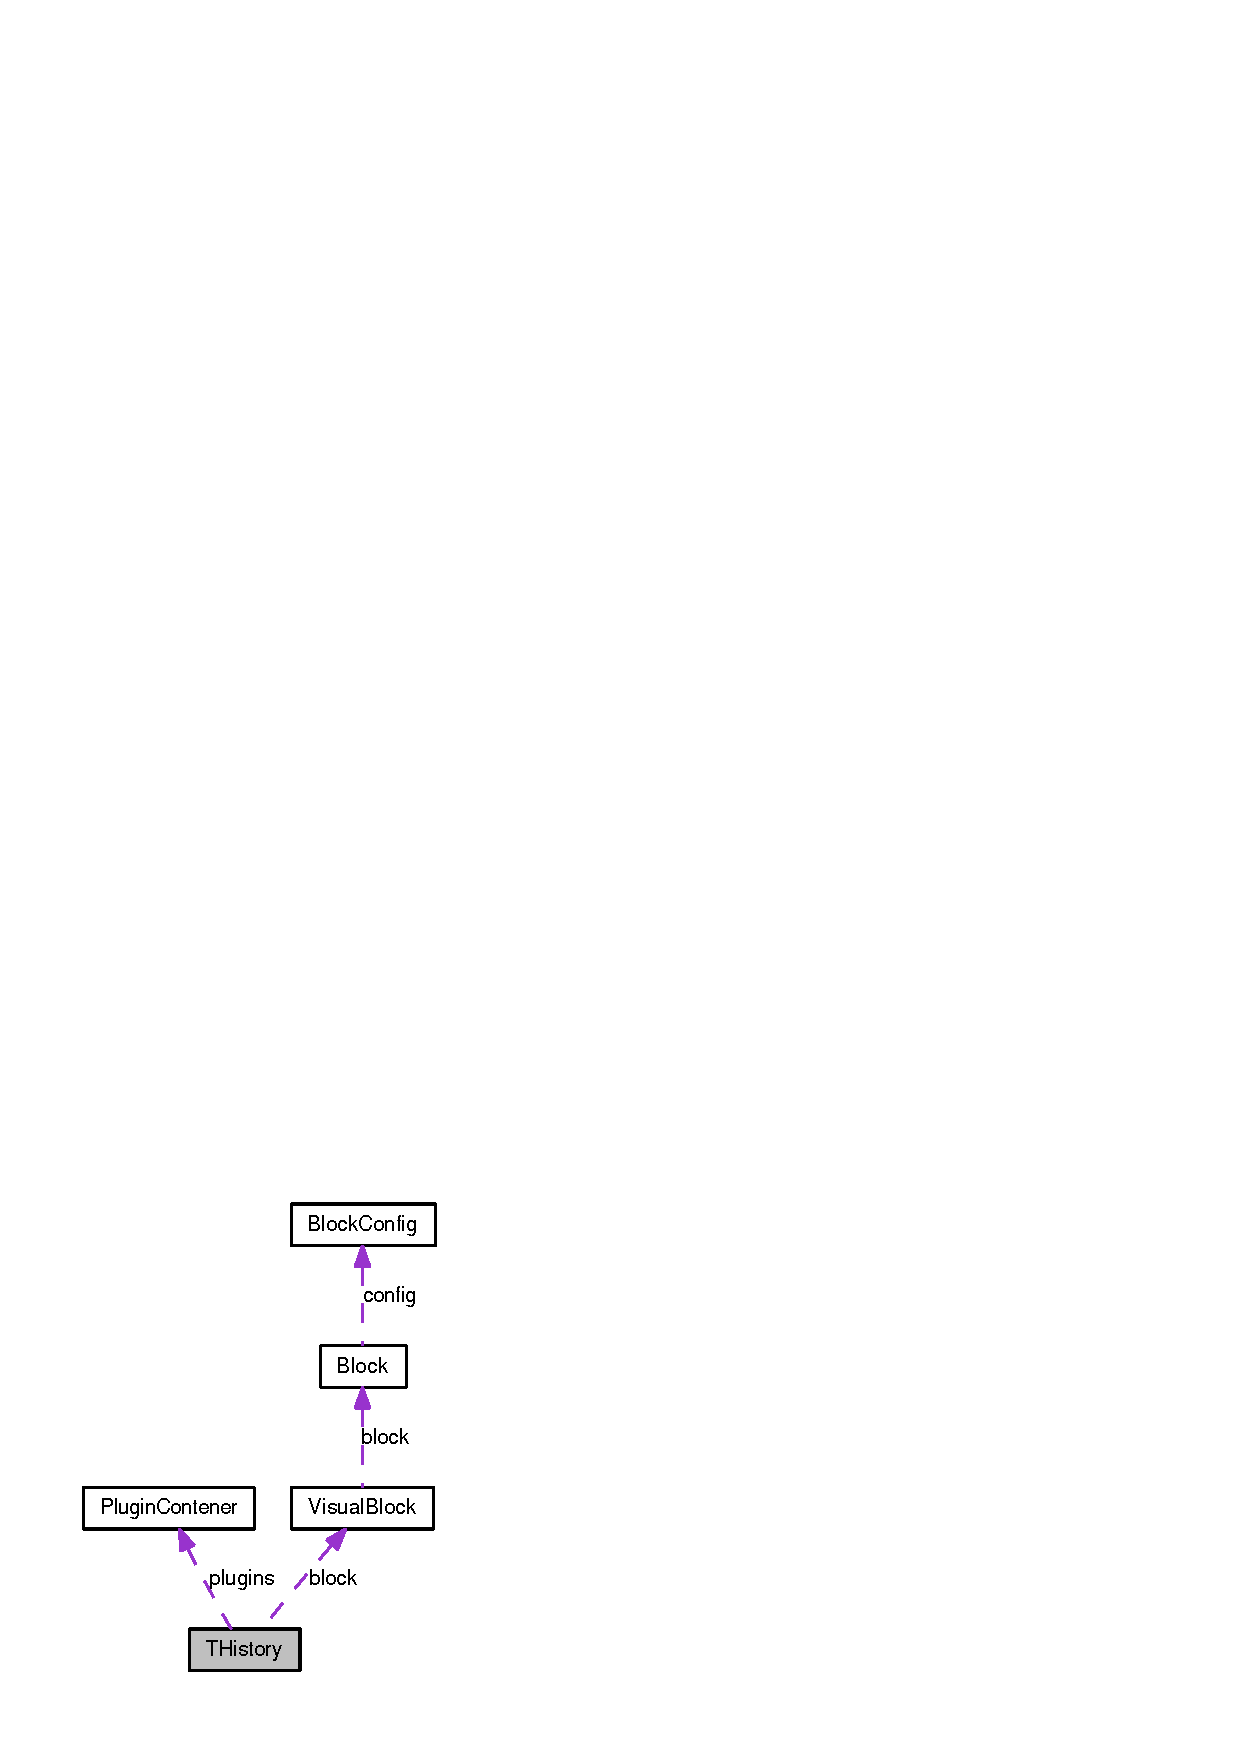
\includegraphics[width=106pt]{classTHistory__coll__graph}
\end{center}
\end{figure}
\subsection*{Public Member Functions}
\begin{CompactItemize}
\item 
void \_\-\_\-fastcall \hyperlink{classTHistory_a54230b362227ac394e19e47471c6ae4}{TreeView1Deletion} (TObject $\ast$Sender, TTreeNode $\ast$Node)
\item 
void \_\-\_\-fastcall \hyperlink{classTHistory_8f2cc8301b158c9845720077b2992b93}{BitBtn2Click} (TObject $\ast$Sender)
\item 
void \_\-\_\-fastcall \hyperlink{classTHistory_4abbf05ae8c7d566b30a7ed0f87fefdf}{TreeView1Click} (TObject $\ast$Sender)
\item 
void \_\-\_\-fastcall \hyperlink{classTHistory_80ff4787a2ecce89533f1fb22cb3c9b6}{CreateParams} (Controls::TCreateParams \&Params)
\item 
\_\-\_\-fastcall \hyperlink{classTHistory_a63049b9a1cc855fc3398c8471e1ca6e}{THistory} (TComponent $\ast$Owner)
\item 
\_\-\_\-fastcall \hyperlink{classTHistory_1aea950a4179841c02848a2f578b6545}{$\sim$THistory} ()
\item 
void \hyperlink{classTHistory_a4c0599263631652e37b50d557269974}{refresh} (\hyperlink{classBlockElement}{BlockElement} $\ast$toShow)
\end{CompactItemize}
\subsection*{Public Attributes}
\begin{CompactItemize}
\item 
TStatusBar $\ast$ \hyperlink{classTHistory_a3f5f2b91a14af33829123e0aaca3928}{StatusBar1}
\item 
TImageList $\ast$ \hyperlink{classTHistory_d1855973aa68d9e9cca14f5632ddfae8}{ImageList1}
\item 
TPanel $\ast$ \hyperlink{classTHistory_4b99f5e227a8e165e6d64be62227c458}{Panel1}
\item 
TTreeView $\ast$ \hyperlink{classTHistory_ce7f826948e9130c7c20d879e7b8d80c}{TreeView1}
\item 
TPanel $\ast$ \hyperlink{classTHistory_628b8da1ed6bee8471e6baa1d8d9911a}{Panel2}
\item 
TBitBtn $\ast$ \hyperlink{classTHistory_58430353f17dbe5b387caabeb221f65b}{BitBtn2}
\item 
TLabel $\ast$ \hyperlink{classTHistory_b308f0efb659683a8d9c7881ca03f2c7}{Label1}
\item 
\hyperlink{classVisualBlock}{VisualBlock} $\ast$ \hyperlink{classTHistory_f4c969766311242d1c6d66cd9b126356}{block}
\item 
\hyperlink{classPluginContener}{PluginContener} $\ast$ \hyperlink{classTHistory_c2d0ea83df40a55b1c899bd87af9652f}{plugins}
\end{CompactItemize}
\subsection*{Private Attributes}
\begin{CompactItemize}
\item 
vector$<$ TForm $\ast$ $>$ \hyperlink{classTHistory_46b9676e3638c8006171026e66f96306}{windows}
\item 
TFrame $\ast$ \hyperlink{classTHistory_bd6410d2b6668ee021fe128e6b7cc874}{showFrame}
\item 
unsigned int \hyperlink{classTHistory_716bcd58a7ba40e8003454d811a64cd0}{count}
\end{CompactItemize}


\subsection{Detailed Description}
Klasa jest oknem histori 

Definition at line 24 of file history.h.

\subsection{Constructor \& Destructor Documentation}
\hypertarget{classTHistory_a63049b9a1cc855fc3398c8471e1ca6e}{
\index{THistory@{THistory}!THistory@{THistory}}
\index{THistory@{THistory}!THistory@{THistory}}
\subsubsection[THistory]{\setlength{\rightskip}{0pt plus 5cm}\_\-\_\-fastcall THistory::THistory (TComponent $\ast$ {\em Owner})}}
\label{classTHistory_a63049b9a1cc855fc3398c8471e1ca6e}


Konstruktor \begin{Desc}
\item[Parameters:]
\begin{description}
\item[{\em Owner}]wskaznik do klasy bedacej wlascicielem dla tej \end{description}
\end{Desc}


Definition at line 8 of file history.cpp.

References count, and showFrame.\hypertarget{classTHistory_1aea950a4179841c02848a2f578b6545}{
\index{THistory@{THistory}!$\sim$THistory@{$\sim$THistory}}
\index{$\sim$THistory@{$\sim$THistory}!THistory@{THistory}}
\subsubsection[$\sim$THistory]{\setlength{\rightskip}{0pt plus 5cm}\_\-\_\-fastcall THistory::$\sim$THistory ()}}
\label{classTHistory_1aea950a4179841c02848a2f578b6545}


Destruktor 

Definition at line 15 of file history.cpp.

References TreeView1.

\subsection{Member Function Documentation}
\hypertarget{classTHistory_a54230b362227ac394e19e47471c6ae4}{
\index{THistory@{THistory}!TreeView1Deletion@{TreeView1Deletion}}
\index{TreeView1Deletion@{TreeView1Deletion}!THistory@{THistory}}
\subsubsection[TreeView1Deletion]{\setlength{\rightskip}{0pt plus 5cm}void \_\-\_\-fastcall THistory::TreeView1Deletion (TObject $\ast$ {\em Sender}, \/  TTreeNode $\ast$ {\em Node})}}
\label{classTHistory_a54230b362227ac394e19e47471c6ae4}




Definition at line 161 of file history.cpp.\hypertarget{classTHistory_8f2cc8301b158c9845720077b2992b93}{
\index{THistory@{THistory}!BitBtn2Click@{BitBtn2Click}}
\index{BitBtn2Click@{BitBtn2Click}!THistory@{THistory}}
\subsubsection[BitBtn2Click]{\setlength{\rightskip}{0pt plus 5cm}void \_\-\_\-fastcall THistory::BitBtn2Click (TObject $\ast$ {\em Sender})}}
\label{classTHistory_8f2cc8301b158c9845720077b2992b93}




Definition at line 171 of file history.cpp.

References refresh().\hypertarget{classTHistory_4abbf05ae8c7d566b30a7ed0f87fefdf}{
\index{THistory@{THistory}!TreeView1Click@{TreeView1Click}}
\index{TreeView1Click@{TreeView1Click}!THistory@{THistory}}
\subsubsection[TreeView1Click]{\setlength{\rightskip}{0pt plus 5cm}void \_\-\_\-fastcall THistory::TreeView1Click (TObject $\ast$ {\em Sender})}}
\label{classTHistory_4abbf05ae8c7d566b30a7ed0f87fefdf}




Definition at line 178 of file history.cpp.

References refresh(), showFrame, and TreeView1.\hypertarget{classTHistory_80ff4787a2ecce89533f1fb22cb3c9b6}{
\index{THistory@{THistory}!CreateParams@{CreateParams}}
\index{CreateParams@{CreateParams}!THistory@{THistory}}
\subsubsection[CreateParams]{\setlength{\rightskip}{0pt plus 5cm}void \_\-\_\-fastcall THistory::CreateParams (Controls::TCreateParams \& {\em Params})}}
\label{classTHistory_80ff4787a2ecce89533f1fb22cb3c9b6}




Definition at line 201 of file history.cpp.\hypertarget{classTHistory_a4c0599263631652e37b50d557269974}{
\index{THistory@{THistory}!refresh@{refresh}}
\index{refresh@{refresh}!THistory@{THistory}}
\subsubsection[refresh]{\setlength{\rightskip}{0pt plus 5cm}void THistory::refresh ({\bf BlockElement} $\ast$ {\em toShow})}}
\label{classTHistory_a4c0599263631652e37b50d557269974}


Metoda wyswietla liste historii, i pokazuje ostatnia historie dla parametru toShow \begin{Desc}
\item[Parameters:]
\begin{description}
\item[{\em toShow}]wskaznik do niskopoziomowego wejscia/wyjscia bloku, jesli NULL to przy wywolaniu zadne \char`\"{}okno\char`\"{} nie zostanie pokazane \end{description}
\end{Desc}


Definition at line 20 of file history.cpp.

References block, count, VisualBlock::getTitle(), PluginContener::getType(), TypeDLL::getType(), VisualBlock::history, Label1, plugins, TypeDLL::show(), showFrame, and TreeView1.

Referenced by BitBtn2Click(), PIWOEngine::OnVisualBlockInputHistoryClick(), PIWOEngine::OnVisualBlockOutputHistoryClick(), and TreeView1Click().

\subsection{Member Data Documentation}
\hypertarget{classTHistory_a3f5f2b91a14af33829123e0aaca3928}{
\index{THistory@{THistory}!StatusBar1@{StatusBar1}}
\index{StatusBar1@{StatusBar1}!THistory@{THistory}}
\subsubsection[StatusBar1]{\setlength{\rightskip}{0pt plus 5cm}TStatusBar$\ast$ {\bf THistory::StatusBar1}}}
\label{classTHistory_a3f5f2b91a14af33829123e0aaca3928}




Definition at line 27 of file history.h.\hypertarget{classTHistory_d1855973aa68d9e9cca14f5632ddfae8}{
\index{THistory@{THistory}!ImageList1@{ImageList1}}
\index{ImageList1@{ImageList1}!THistory@{THistory}}
\subsubsection[ImageList1]{\setlength{\rightskip}{0pt plus 5cm}TImageList$\ast$ {\bf THistory::ImageList1}}}
\label{classTHistory_d1855973aa68d9e9cca14f5632ddfae8}




Definition at line 28 of file history.h.\hypertarget{classTHistory_4b99f5e227a8e165e6d64be62227c458}{
\index{THistory@{THistory}!Panel1@{Panel1}}
\index{Panel1@{Panel1}!THistory@{THistory}}
\subsubsection[Panel1]{\setlength{\rightskip}{0pt plus 5cm}TPanel$\ast$ {\bf THistory::Panel1}}}
\label{classTHistory_4b99f5e227a8e165e6d64be62227c458}




Definition at line 29 of file history.h.\hypertarget{classTHistory_ce7f826948e9130c7c20d879e7b8d80c}{
\index{THistory@{THistory}!TreeView1@{TreeView1}}
\index{TreeView1@{TreeView1}!THistory@{THistory}}
\subsubsection[TreeView1]{\setlength{\rightskip}{0pt plus 5cm}TTreeView$\ast$ {\bf THistory::TreeView1}}}
\label{classTHistory_ce7f826948e9130c7c20d879e7b8d80c}




Definition at line 30 of file history.h.

Referenced by refresh(), TreeView1Click(), and $\sim$THistory().\hypertarget{classTHistory_628b8da1ed6bee8471e6baa1d8d9911a}{
\index{THistory@{THistory}!Panel2@{Panel2}}
\index{Panel2@{Panel2}!THistory@{THistory}}
\subsubsection[Panel2]{\setlength{\rightskip}{0pt plus 5cm}TPanel$\ast$ {\bf THistory::Panel2}}}
\label{classTHistory_628b8da1ed6bee8471e6baa1d8d9911a}




Definition at line 31 of file history.h.\hypertarget{classTHistory_58430353f17dbe5b387caabeb221f65b}{
\index{THistory@{THistory}!BitBtn2@{BitBtn2}}
\index{BitBtn2@{BitBtn2}!THistory@{THistory}}
\subsubsection[BitBtn2]{\setlength{\rightskip}{0pt plus 5cm}TBitBtn$\ast$ {\bf THistory::BitBtn2}}}
\label{classTHistory_58430353f17dbe5b387caabeb221f65b}




Definition at line 32 of file history.h.\hypertarget{classTHistory_b308f0efb659683a8d9c7881ca03f2c7}{
\index{THistory@{THistory}!Label1@{Label1}}
\index{Label1@{Label1}!THistory@{THistory}}
\subsubsection[Label1]{\setlength{\rightskip}{0pt plus 5cm}TLabel$\ast$ {\bf THistory::Label1}}}
\label{classTHistory_b308f0efb659683a8d9c7881ca03f2c7}




Definition at line 33 of file history.h.

Referenced by refresh().\hypertarget{classTHistory_46b9676e3638c8006171026e66f96306}{
\index{THistory@{THistory}!windows@{windows}}
\index{windows@{windows}!THistory@{THistory}}
\subsubsection[windows]{\setlength{\rightskip}{0pt plus 5cm}vector$<$TForm$\ast$$>$ {\bf THistory::windows}\hspace{0.3cm}{\tt  \mbox{[}private\mbox{]}}}}
\label{classTHistory_46b9676e3638c8006171026e66f96306}




Definition at line 39 of file history.h.\hypertarget{classTHistory_bd6410d2b6668ee021fe128e6b7cc874}{
\index{THistory@{THistory}!showFrame@{showFrame}}
\index{showFrame@{showFrame}!THistory@{THistory}}
\subsubsection[showFrame]{\setlength{\rightskip}{0pt plus 5cm}TFrame$\ast$ {\bf THistory::showFrame}\hspace{0.3cm}{\tt  \mbox{[}private\mbox{]}}}}
\label{classTHistory_bd6410d2b6668ee021fe128e6b7cc874}




Definition at line 40 of file history.h.

Referenced by refresh(), THistory(), and TreeView1Click().\hypertarget{classTHistory_716bcd58a7ba40e8003454d811a64cd0}{
\index{THistory@{THistory}!count@{count}}
\index{count@{count}!THistory@{THistory}}
\subsubsection[count]{\setlength{\rightskip}{0pt plus 5cm}unsigned int {\bf THistory::count}\hspace{0.3cm}{\tt  \mbox{[}private\mbox{]}}}}
\label{classTHistory_716bcd58a7ba40e8003454d811a64cd0}




Definition at line 41 of file history.h.

Referenced by refresh(), and THistory().\hypertarget{classTHistory_f4c969766311242d1c6d66cd9b126356}{
\index{THistory@{THistory}!block@{block}}
\index{block@{block}!THistory@{THistory}}
\subsubsection[block]{\setlength{\rightskip}{0pt plus 5cm}{\bf VisualBlock}$\ast$ {\bf THistory::block}}}
\label{classTHistory_f4c969766311242d1c6d66cd9b126356}


Wskaznik do wizualnego bloku, musi byc ustawiony przed refresh 

Definition at line 55 of file history.h.

Referenced by PIWOEngine::OnVisualBlockInputHistoryClick(), PIWOEngine::OnVisualBlockOutputHistoryClick(), and refresh().\hypertarget{classTHistory_c2d0ea83df40a55b1c899bd87af9652f}{
\index{THistory@{THistory}!plugins@{plugins}}
\index{plugins@{plugins}!THistory@{THistory}}
\subsubsection[plugins]{\setlength{\rightskip}{0pt plus 5cm}{\bf PluginContener}$\ast$ {\bf THistory::plugins}}}
\label{classTHistory_c2d0ea83df40a55b1c899bd87af9652f}


Wskaznik do kontenera pluginow, musi byc ustawione przed refresh 

Definition at line 59 of file history.h.

Referenced by PIWOEngine::OnVisualBlockInputHistoryClick(), PIWOEngine::OnVisualBlockOutputHistoryClick(), and refresh().

The documentation for this class was generated from the following files:\begin{CompactItemize}
\item 
/PIWO/Program/gui/\hyperlink{history_8h}{history.h}\item 
/PIWO/Program/gui/\hyperlink{history_8cpp}{history.cpp}\end{CompactItemize}

\hypertarget{classTypeConfig}{
\section{TypeConfig Class Reference}
\label{classTypeConfig}\index{TypeConfig@{TypeConfig}}
}
{\tt \#include $<$TypeConfig.h$>$}

Inheritance diagram for TypeConfig:\nopagebreak
\begin{figure}[H]
\begin{center}
\leavevmode
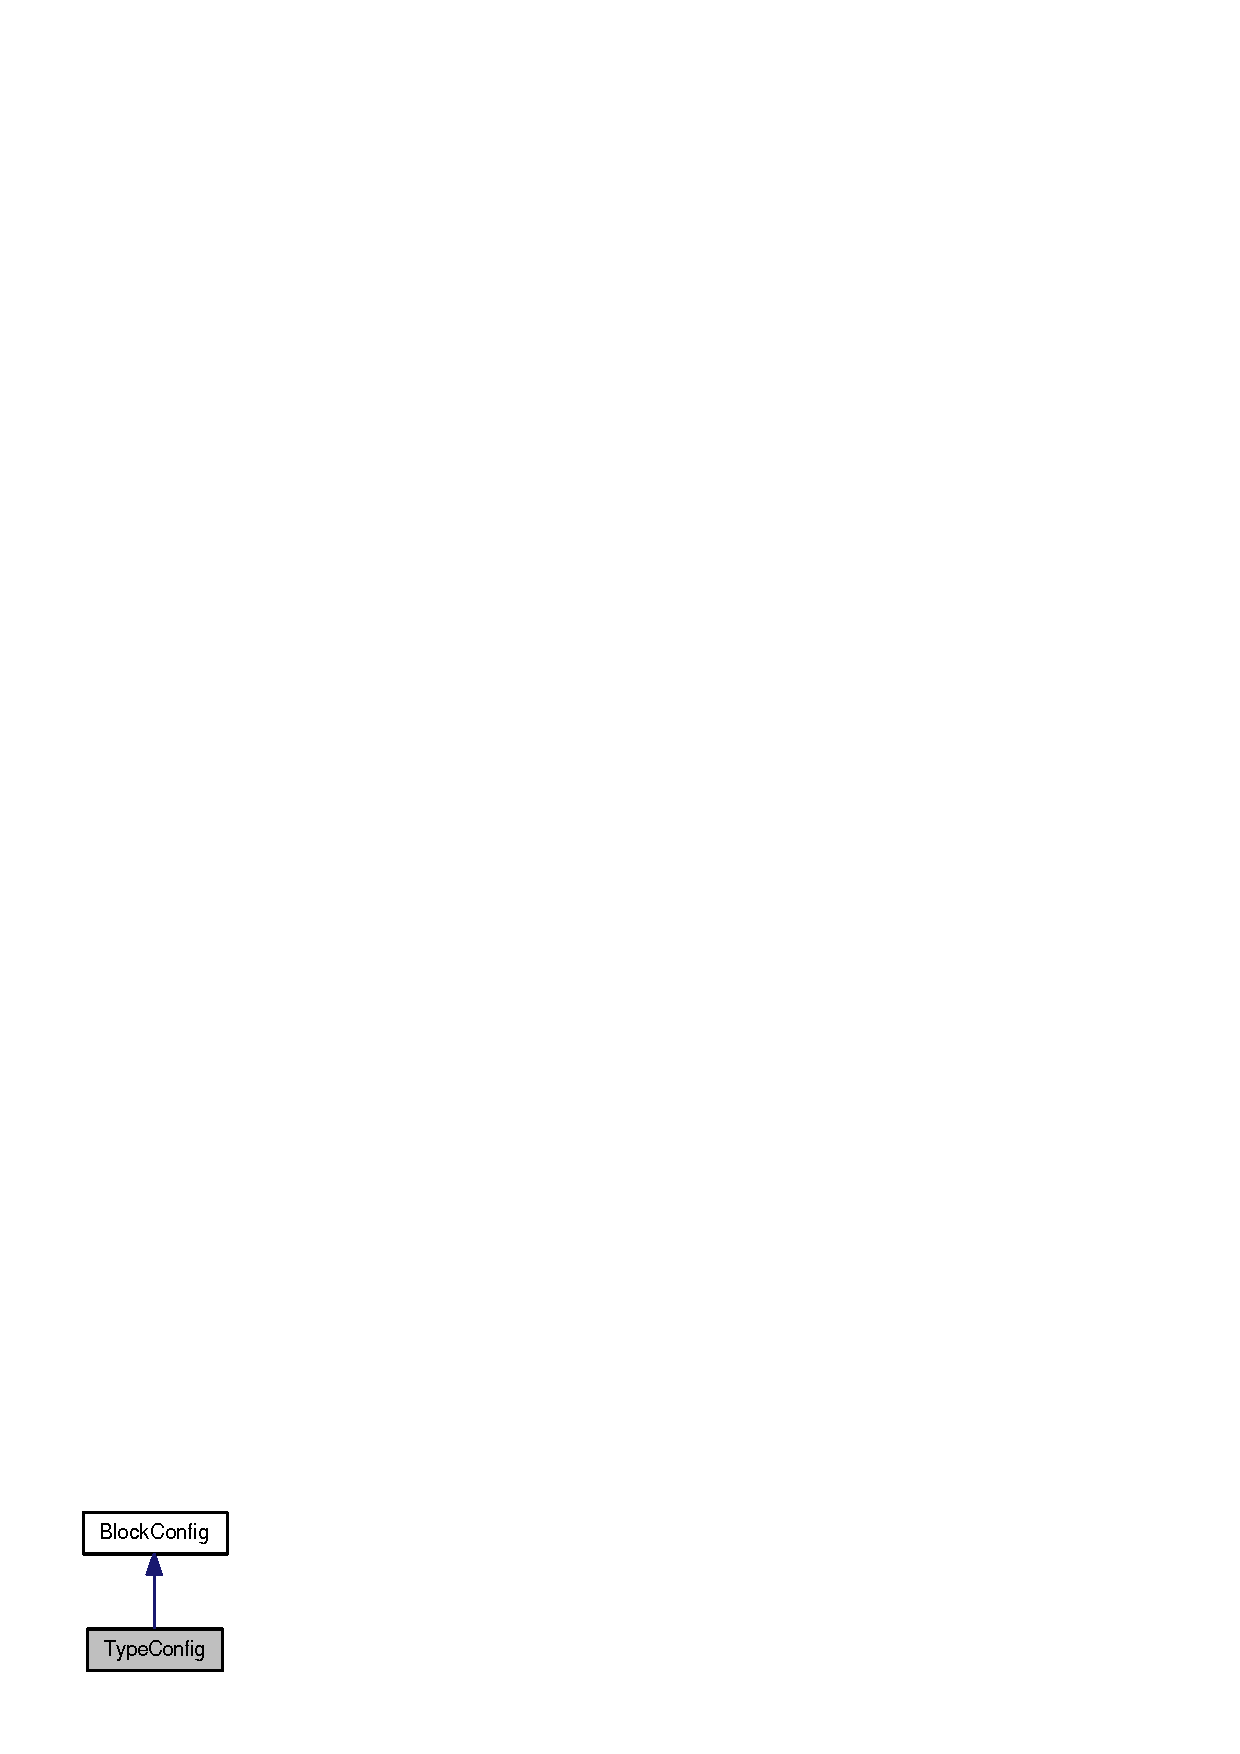
\includegraphics[width=56pt]{classTypeConfig__inherit__graph}
\end{center}
\end{figure}
Collaboration diagram for TypeConfig:\nopagebreak
\begin{figure}[H]
\begin{center}
\leavevmode
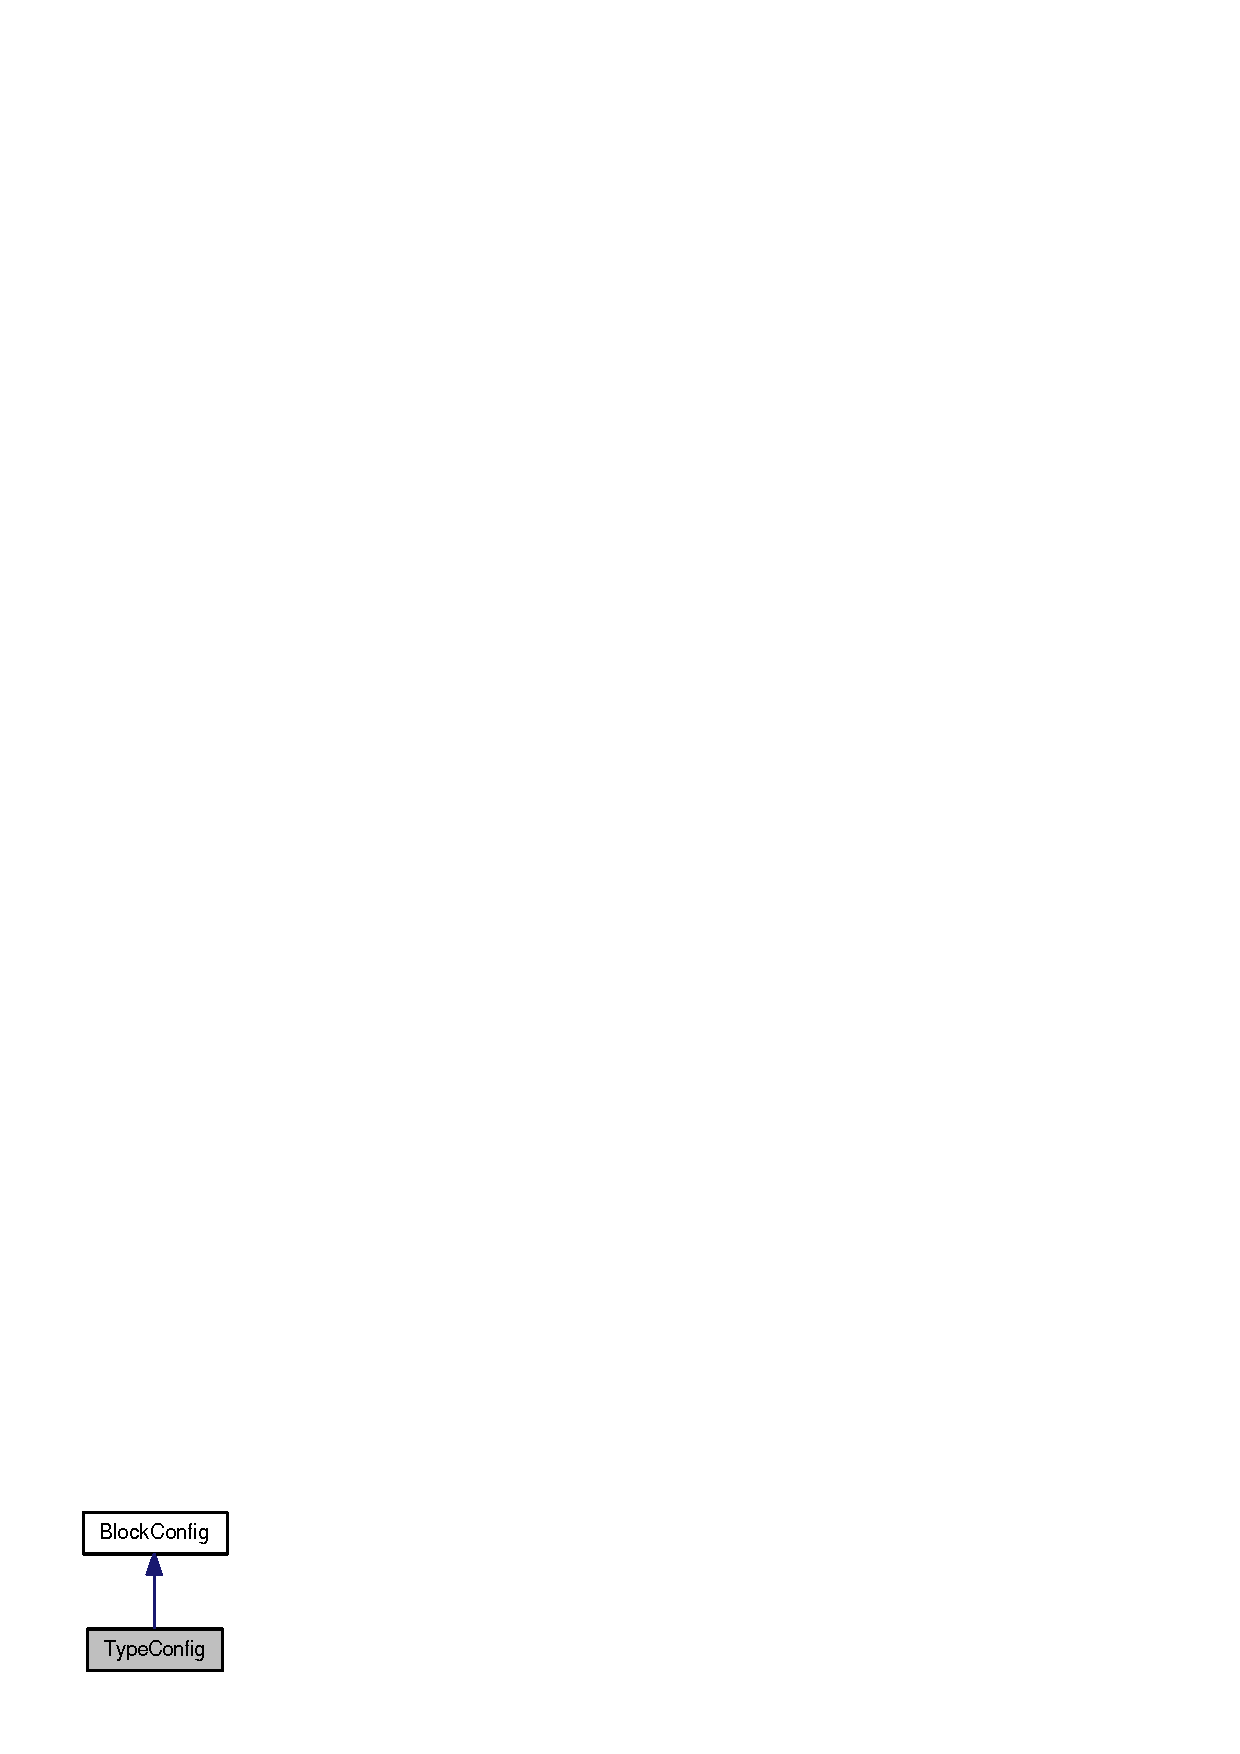
\includegraphics[width=56pt]{classTypeConfig__coll__graph}
\end{center}
\end{figure}
\subsection*{Public Member Functions}
\begin{CompactItemize}
\item 
\hyperlink{classTypeConfig_b2a221c2d5bf396018399269dd3f3e9d}{TypeConfig} (const AnsiString aName)
\item 
\hyperlink{classTypeConfig_e8b6161a3b6b8a1a9991f7240a2ec7a2}{TypeConfig} (const \hyperlink{classTypeConfig}{TypeConfig} \&kopia)
\item 
\hyperlink{classTypeConfig_77929bc854791d0879ab952eef688b8f}{TypeConfig} (TStream \&stream)
\item 
\hyperlink{classTypeConfig_dfc381c0e5957f32637705ecb900a34c}{$\sim$TypeConfig} ()
\item 
bool \hyperlink{classTypeConfig_6d8e08fc2726691b9fd49753504125b2}{saveToStream} (TStream \&aWhere)
\item 
bool \hyperlink{classTypeConfig_3ea873062f9be5fbc1001503684f532d}{loadFromStream} (TStream \&aFrom)
\item 
const AnsiString \& \hyperlink{classTypeConfig_def1a09e268a7929a3be7529272824c5}{getName} ()
\item 
unsigned long \hyperlink{classTypeConfig_c71d61eebbe3f8a18b9615b670e0a1d3}{getId} ()
\end{CompactItemize}
\subsection*{Protected Attributes}
\begin{CompactItemize}
\item 
AnsiString \hyperlink{classTypeConfig_de545d5c97e90206890ff72a02d2465c}{nazwa}
\item 
unsigned long \hyperlink{classTypeConfig_2feac272551cd0f837f7a8d3d9ca8034}{id}
\end{CompactItemize}


\subsection{Detailed Description}
\hyperlink{classTypeConfig}{TypeConfig} - Klasa reprezentujaca typ przesylany do bloku zdefiniowany przez uzytkownika. \begin{Desc}
\item[Author:]Piotr \end{Desc}
\begin{Desc}
\item[Date:]2008.11.25 \end{Desc}
\begin{Desc}
\item[Version:]0.1 \end{Desc}


Definition at line 16 of file TypeConfig.h.

\subsection{Constructor \& Destructor Documentation}
\hypertarget{classTypeConfig_b2a221c2d5bf396018399269dd3f3e9d}{
\index{TypeConfig@{TypeConfig}!TypeConfig@{TypeConfig}}
\index{TypeConfig@{TypeConfig}!TypeConfig@{TypeConfig}}
\subsubsection[TypeConfig]{\setlength{\rightskip}{0pt plus 5cm}TypeConfig::TypeConfig (const AnsiString {\em aName})}}
\label{classTypeConfig_b2a221c2d5bf396018399269dd3f3e9d}


Konstruktor \begin{Desc}
\item[Parameters:]
\begin{description}
\item[{\em aName}]- nazwa nowego typu. \end{description}
\end{Desc}


Definition at line 8 of file TypeConfig.cpp.

References nazwa.\hypertarget{classTypeConfig_e8b6161a3b6b8a1a9991f7240a2ec7a2}{
\index{TypeConfig@{TypeConfig}!TypeConfig@{TypeConfig}}
\index{TypeConfig@{TypeConfig}!TypeConfig@{TypeConfig}}
\subsubsection[TypeConfig]{\setlength{\rightskip}{0pt plus 5cm}TypeConfig::TypeConfig (const {\bf TypeConfig} \& {\em kopia})}}
\label{classTypeConfig_e8b6161a3b6b8a1a9991f7240a2ec7a2}


Konstruktor kopiujacy. \begin{Desc}
\item[Parameters:]
\begin{description}
\item[{\em kopia}]obiekt ktory zostanie skopiowany \end{description}
\end{Desc}


Definition at line 22 of file TypeConfig.cpp.

References id, and nazwa.\hypertarget{classTypeConfig_77929bc854791d0879ab952eef688b8f}{
\index{TypeConfig@{TypeConfig}!TypeConfig@{TypeConfig}}
\index{TypeConfig@{TypeConfig}!TypeConfig@{TypeConfig}}
\subsubsection[TypeConfig]{\setlength{\rightskip}{0pt plus 5cm}TypeConfig::TypeConfig (TStream \& {\em stream})}}
\label{classTypeConfig_77929bc854791d0879ab952eef688b8f}


Konstruktor \begin{Desc}
\item[Parameters:]
\begin{description}
\item[{\em stream}]- strumien z ktorego zostana odczytane dane. \end{description}
\end{Desc}


Definition at line 16 of file TypeConfig.cpp.

References loadFromStream().\hypertarget{classTypeConfig_dfc381c0e5957f32637705ecb900a34c}{
\index{TypeConfig@{TypeConfig}!$\sim$TypeConfig@{$\sim$TypeConfig}}
\index{$\sim$TypeConfig@{$\sim$TypeConfig}!TypeConfig@{TypeConfig}}
\subsubsection[$\sim$TypeConfig]{\setlength{\rightskip}{0pt plus 5cm}TypeConfig::$\sim$TypeConfig ()}}
\label{classTypeConfig_dfc381c0e5957f32637705ecb900a34c}


Destruktor 

Definition at line 28 of file TypeConfig.cpp.

\subsection{Member Function Documentation}
\hypertarget{classTypeConfig_6d8e08fc2726691b9fd49753504125b2}{
\index{TypeConfig@{TypeConfig}!saveToStream@{saveToStream}}
\index{saveToStream@{saveToStream}!TypeConfig@{TypeConfig}}
\subsubsection[saveToStream]{\setlength{\rightskip}{0pt plus 5cm}bool TypeConfig::saveToStream (TStream \& {\em aWhere})}}
\label{classTypeConfig_6d8e08fc2726691b9fd49753504125b2}


Zapisuje list� obiektow do strumienia. \begin{Desc}
\item[Parameters:]
\begin{description}
\item[{\em aWhere}]strumien w ktorym zostana zapisane informacje. \end{description}
\end{Desc}
\begin{Desc}
\item[Returns:]true - jezeli operacja sie powiodla false - jezeli nie. \end{Desc}


Reimplemented from \hyperlink{classBlockConfig_78a3531c448dca0bd61f57fc2034a5c0}{BlockConfig}.

Definition at line 33 of file TypeConfig.cpp.

References id, nazwa, and BlockConfig::saveToStream2().\hypertarget{classTypeConfig_3ea873062f9be5fbc1001503684f532d}{
\index{TypeConfig@{TypeConfig}!loadFromStream@{loadFromStream}}
\index{loadFromStream@{loadFromStream}!TypeConfig@{TypeConfig}}
\subsubsection[loadFromStream]{\setlength{\rightskip}{0pt plus 5cm}bool TypeConfig::loadFromStream (TStream \& {\em aFrom})}}
\label{classTypeConfig_3ea873062f9be5fbc1001503684f532d}


Odczytuje infomracj� o obiektach na liscie z strumienia \begin{Desc}
\item[Parameters:]
\begin{description}
\item[{\em aName}]nazwa obiektu \end{description}
\end{Desc}
\begin{Desc}
\item[Returns:]true - jezeli operacja sie powiodla false - jezeli nie. \end{Desc}


Reimplemented from \hyperlink{classBlockConfig_fa1e7a52f16ebcb1ceed3b33c5a9734e}{BlockConfig}.

Definition at line 48 of file TypeConfig.cpp.

References BlockConfig::clear(), BlockConfig::loadFromStream2(), and nazwa.

Referenced by TypeConfig().\hypertarget{classTypeConfig_def1a09e268a7929a3be7529272824c5}{
\index{TypeConfig@{TypeConfig}!getName@{getName}}
\index{getName@{getName}!TypeConfig@{TypeConfig}}
\subsubsection[getName]{\setlength{\rightskip}{0pt plus 5cm}const AnsiString \& TypeConfig::getName ()}}
\label{classTypeConfig_def1a09e268a7929a3be7529272824c5}


Pobiera nazwe. \begin{Desc}
\item[Returns:]nazwa obiektu. \end{Desc}


Definition at line 66 of file TypeConfig.cpp.

References nazwa.

Referenced by PIWOEngine::runBlock().\hypertarget{classTypeConfig_c71d61eebbe3f8a18b9615b670e0a1d3}{
\index{TypeConfig@{TypeConfig}!getId@{getId}}
\index{getId@{getId}!TypeConfig@{TypeConfig}}
\subsubsection[getId]{\setlength{\rightskip}{0pt plus 5cm}unsigned long TypeConfig::getId ()}}
\label{classTypeConfig_c71d61eebbe3f8a18b9615b670e0a1d3}


Zwraca unikalny id dla tej klasy, jest nim adres w pamieci pod ktorym zostala stworzona 

Definition at line 71 of file TypeConfig.cpp.

References id.

\subsection{Member Data Documentation}
\hypertarget{classTypeConfig_de545d5c97e90206890ff72a02d2465c}{
\index{TypeConfig@{TypeConfig}!nazwa@{nazwa}}
\index{nazwa@{nazwa}!TypeConfig@{TypeConfig}}
\subsubsection[nazwa]{\setlength{\rightskip}{0pt plus 5cm}AnsiString {\bf TypeConfig::nazwa}\hspace{0.3cm}{\tt  \mbox{[}protected\mbox{]}}}}
\label{classTypeConfig_de545d5c97e90206890ff72a02d2465c}




Definition at line 19 of file TypeConfig.h.

Referenced by getName(), loadFromStream(), saveToStream(), and TypeConfig().\hypertarget{classTypeConfig_2feac272551cd0f837f7a8d3d9ca8034}{
\index{TypeConfig@{TypeConfig}!id@{id}}
\index{id@{id}!TypeConfig@{TypeConfig}}
\subsubsection[id]{\setlength{\rightskip}{0pt plus 5cm}unsigned long {\bf TypeConfig::id}\hspace{0.3cm}{\tt  \mbox{[}protected\mbox{]}}}}
\label{classTypeConfig_2feac272551cd0f837f7a8d3d9ca8034}




Definition at line 20 of file TypeConfig.h.

Referenced by getId(), saveToStream(), and TypeConfig().

The documentation for this class was generated from the following files:\begin{CompactItemize}
\item 
/PIWO/Program/engine/\hyperlink{TypeConfig_8h}{TypeConfig.h}\item 
/PIWO/Program/engine/\hyperlink{TypeConfig_8cpp}{TypeConfig.cpp}\end{CompactItemize}

\hypertarget{classTypeDLL}{
\section{TypeDLL Class Reference}
\label{classTypeDLL}\index{TypeDLL@{TypeDLL}}
}
{\tt \#include $<$TypeDLL.h$>$}

\subsection*{Public Member Functions}
\begin{CompactItemize}
\item 
\hyperlink{classTypeDLL_ab72ed838b47da3b97580120be8b9089}{TypeDLL} (const AnsiString \&fileDLL)
\item 
\hyperlink{classTypeDLL_a4c2e51a5ceb30a96c1b9d5afba93603}{$\sim$TypeDLL} ()
\item 
TFrame $\ast$ \hyperlink{classTypeDLL_67cdb99638bd6af8ec8156bad8e9b3d0}{show} (TWinControl $\ast$parent, \hyperlink{classTypeConfig}{TypeConfig} $\ast$aData)
\item 
bool \hyperlink{classTypeDLL_b6478c39cb533da91e2b0a3f045067d5}{isValid} (\hyperlink{classTypeConfig}{TypeConfig} $\ast$aData)
\item 
AnsiString \hyperlink{classTypeDLL_28c8d6824e3c12c04ae91e43f27fc34b}{getType} ()
\end{CompactItemize}
\subsection*{Private Attributes}
\begin{CompactItemize}
\item 
AnsiString \hyperlink{classTypeDLL_bae421811d0fefe89c4bba6d21474a7a}{type}
\item 
HANDLE \hyperlink{classTypeDLL_90d9ea7c7fd718d235f77d300bc572a5}{DLLHandle}
\item 
\hyperlink{TypeDLL_8h_e3b92b079373f3c0fae8106774b2c686}{TypeDLL\_\-show} \hyperlink{classTypeDLL_bb1bda3b0b147c761e5354d5ed856c1b}{fshow}
\item 
TypeDLL\_\-isValid \hyperlink{classTypeDLL_7f0d7546e2f0c211ad2d70b2dc416540}{fisValid}
\item 
TypeDLL\_\-getType \hyperlink{classTypeDLL_66b6a0fb2e18a432f2c59bd055c688d3}{fgetType}
\end{CompactItemize}


\subsection{Detailed Description}
Interfejs pozwalajacy na l�dowanie i uzywanie biblioteki typu \begin{Desc}
\item[Author:]Piotr \end{Desc}
\begin{Desc}
\item[Date:]2008.11.25 \end{Desc}
\begin{Desc}
\item[Version:]0.1 \end{Desc}


Definition at line 21 of file TypeDLL.h.

\subsection{Constructor \& Destructor Documentation}
\hypertarget{classTypeDLL_ab72ed838b47da3b97580120be8b9089}{
\index{TypeDLL@{TypeDLL}!TypeDLL@{TypeDLL}}
\index{TypeDLL@{TypeDLL}!TypeDLL@{TypeDLL}}
\subsubsection[TypeDLL]{\setlength{\rightskip}{0pt plus 5cm}TypeDLL::TypeDLL (const AnsiString \& {\em fileDLL})}}
\label{classTypeDLL_ab72ed838b47da3b97580120be8b9089}


Konstruktor \begin{Desc}
\item[Parameters:]
\begin{description}
\item[{\em file}]sciezka do pliku \item[{\em stype}]\end{description}
\end{Desc}


Definition at line 3 of file TypeDLL.cpp.

References DLLHandle, fgetType, fisValid, and fshow.\hypertarget{classTypeDLL_a4c2e51a5ceb30a96c1b9d5afba93603}{
\index{TypeDLL@{TypeDLL}!$\sim$TypeDLL@{$\sim$TypeDLL}}
\index{$\sim$TypeDLL@{$\sim$TypeDLL}!TypeDLL@{TypeDLL}}
\subsubsection[$\sim$TypeDLL]{\setlength{\rightskip}{0pt plus 5cm}TypeDLL::$\sim$TypeDLL ()}}
\label{classTypeDLL_a4c2e51a5ceb30a96c1b9d5afba93603}


Destruktor 

Definition at line 17 of file TypeDLL.cpp.

References DLLHandle.

\subsection{Member Function Documentation}
\hypertarget{classTypeDLL_67cdb99638bd6af8ec8156bad8e9b3d0}{
\index{TypeDLL@{TypeDLL}!show@{show}}
\index{show@{show}!TypeDLL@{TypeDLL}}
\subsubsection[show]{\setlength{\rightskip}{0pt plus 5cm}TFrame $\ast$ TypeDLL::show (TWinControl $\ast$ {\em parent}, \/  {\bf TypeConfig} $\ast$ {\em aData})}}
\label{classTypeDLL_67cdb99638bd6af8ec8156bad8e9b3d0}


Wykonuje funkcje show w zaladowanej DLL typu \begin{Desc}
\item[Parameters:]
\begin{description}
\item[{\em parent}]wskaznik na obiekt wizualny ktory ma zostac uznany za parent - powinno to byc okno \item[{\em aData}]dane \end{description}
\end{Desc}
\begin{Desc}
\item[Returns:]zwraca wskaznik na obiekt TFrame, naszym obowiaskiem jest prawidlowo zwolnic go. \end{Desc}


Definition at line 22 of file TypeDLL.cpp.

References fshow.

Referenced by THistory::refresh().\hypertarget{classTypeDLL_b6478c39cb533da91e2b0a3f045067d5}{
\index{TypeDLL@{TypeDLL}!isValid@{isValid}}
\index{isValid@{isValid}!TypeDLL@{TypeDLL}}
\subsubsection[isValid]{\setlength{\rightskip}{0pt plus 5cm}bool TypeDLL::isValid ({\bf TypeConfig} $\ast$ {\em aData})}}
\label{classTypeDLL_b6478c39cb533da91e2b0a3f045067d5}


Sprawdza poprawnosc danych. \begin{Desc}
\item[Parameters:]
\begin{description}
\item[{\em aData}]dane. \end{description}
\end{Desc}
\begin{Desc}
\item[Returns:]poprawnosc wykonanej operacji \end{Desc}


Definition at line 26 of file TypeDLL.cpp.

References fisValid.

Referenced by PIWOEngine::runBlock().\hypertarget{classTypeDLL_28c8d6824e3c12c04ae91e43f27fc34b}{
\index{TypeDLL@{TypeDLL}!getType@{getType}}
\index{getType@{getType}!TypeDLL@{TypeDLL}}
\subsubsection[getType]{\setlength{\rightskip}{0pt plus 5cm}AnsiString TypeDLL::getType ()}}
\label{classTypeDLL_28c8d6824e3c12c04ae91e43f27fc34b}


Pobiera typ. \begin{Desc}
\item[Returns:]typ. \end{Desc}


Definition at line 30 of file TypeDLL.cpp.

References fgetType.

Referenced by PluginContener::LoadData(), THistory::refresh(), and PIWOEngine::runBlock().

\subsection{Member Data Documentation}
\hypertarget{classTypeDLL_bae421811d0fefe89c4bba6d21474a7a}{
\index{TypeDLL@{TypeDLL}!type@{type}}
\index{type@{type}!TypeDLL@{TypeDLL}}
\subsubsection[type]{\setlength{\rightskip}{0pt plus 5cm}AnsiString {\bf TypeDLL::type}\hspace{0.3cm}{\tt  \mbox{[}private\mbox{]}}}}
\label{classTypeDLL_bae421811d0fefe89c4bba6d21474a7a}




Definition at line 24 of file TypeDLL.h.\hypertarget{classTypeDLL_90d9ea7c7fd718d235f77d300bc572a5}{
\index{TypeDLL@{TypeDLL}!DLLHandle@{DLLHandle}}
\index{DLLHandle@{DLLHandle}!TypeDLL@{TypeDLL}}
\subsubsection[DLLHandle]{\setlength{\rightskip}{0pt plus 5cm}HANDLE {\bf TypeDLL::DLLHandle}\hspace{0.3cm}{\tt  \mbox{[}private\mbox{]}}}}
\label{classTypeDLL_90d9ea7c7fd718d235f77d300bc572a5}




Definition at line 25 of file TypeDLL.h.

Referenced by TypeDLL(), and $\sim$TypeDLL().\hypertarget{classTypeDLL_bb1bda3b0b147c761e5354d5ed856c1b}{
\index{TypeDLL@{TypeDLL}!fshow@{fshow}}
\index{fshow@{fshow}!TypeDLL@{TypeDLL}}
\subsubsection[fshow]{\setlength{\rightskip}{0pt plus 5cm}{\bf TypeDLL\_\-show} {\bf TypeDLL::fshow}\hspace{0.3cm}{\tt  \mbox{[}private\mbox{]}}}}
\label{classTypeDLL_bb1bda3b0b147c761e5354d5ed856c1b}




Definition at line 26 of file TypeDLL.h.

Referenced by show(), and TypeDLL().\hypertarget{classTypeDLL_7f0d7546e2f0c211ad2d70b2dc416540}{
\index{TypeDLL@{TypeDLL}!fisValid@{fisValid}}
\index{fisValid@{fisValid}!TypeDLL@{TypeDLL}}
\subsubsection[fisValid]{\setlength{\rightskip}{0pt plus 5cm}TypeDLL\_\-isValid {\bf TypeDLL::fisValid}\hspace{0.3cm}{\tt  \mbox{[}private\mbox{]}}}}
\label{classTypeDLL_7f0d7546e2f0c211ad2d70b2dc416540}




Definition at line 27 of file TypeDLL.h.

Referenced by isValid(), and TypeDLL().\hypertarget{classTypeDLL_66b6a0fb2e18a432f2c59bd055c688d3}{
\index{TypeDLL@{TypeDLL}!fgetType@{fgetType}}
\index{fgetType@{fgetType}!TypeDLL@{TypeDLL}}
\subsubsection[fgetType]{\setlength{\rightskip}{0pt plus 5cm}TypeDLL\_\-getType {\bf TypeDLL::fgetType}\hspace{0.3cm}{\tt  \mbox{[}private\mbox{]}}}}
\label{classTypeDLL_66b6a0fb2e18a432f2c59bd055c688d3}




Definition at line 28 of file TypeDLL.h.

Referenced by getType(), and TypeDLL().

The documentation for this class was generated from the following files:\begin{CompactItemize}
\item 
/PIWO/Program/brige/\hyperlink{TypeDLL_8h}{TypeDLL.h}\item 
/PIWO/Program/brige/\hyperlink{TypeDLL_8cpp}{TypeDLL.cpp}\end{CompactItemize}

\hypertarget{classVisualBlock}{
\section{VisualBlock Class Reference}
\label{classVisualBlock}\index{VisualBlock@{VisualBlock}}
}
{\tt \#include $<$VisualBlock.h$>$}

Collaboration diagram for VisualBlock:\nopagebreak
\begin{figure}[H]
\begin{center}
\leavevmode
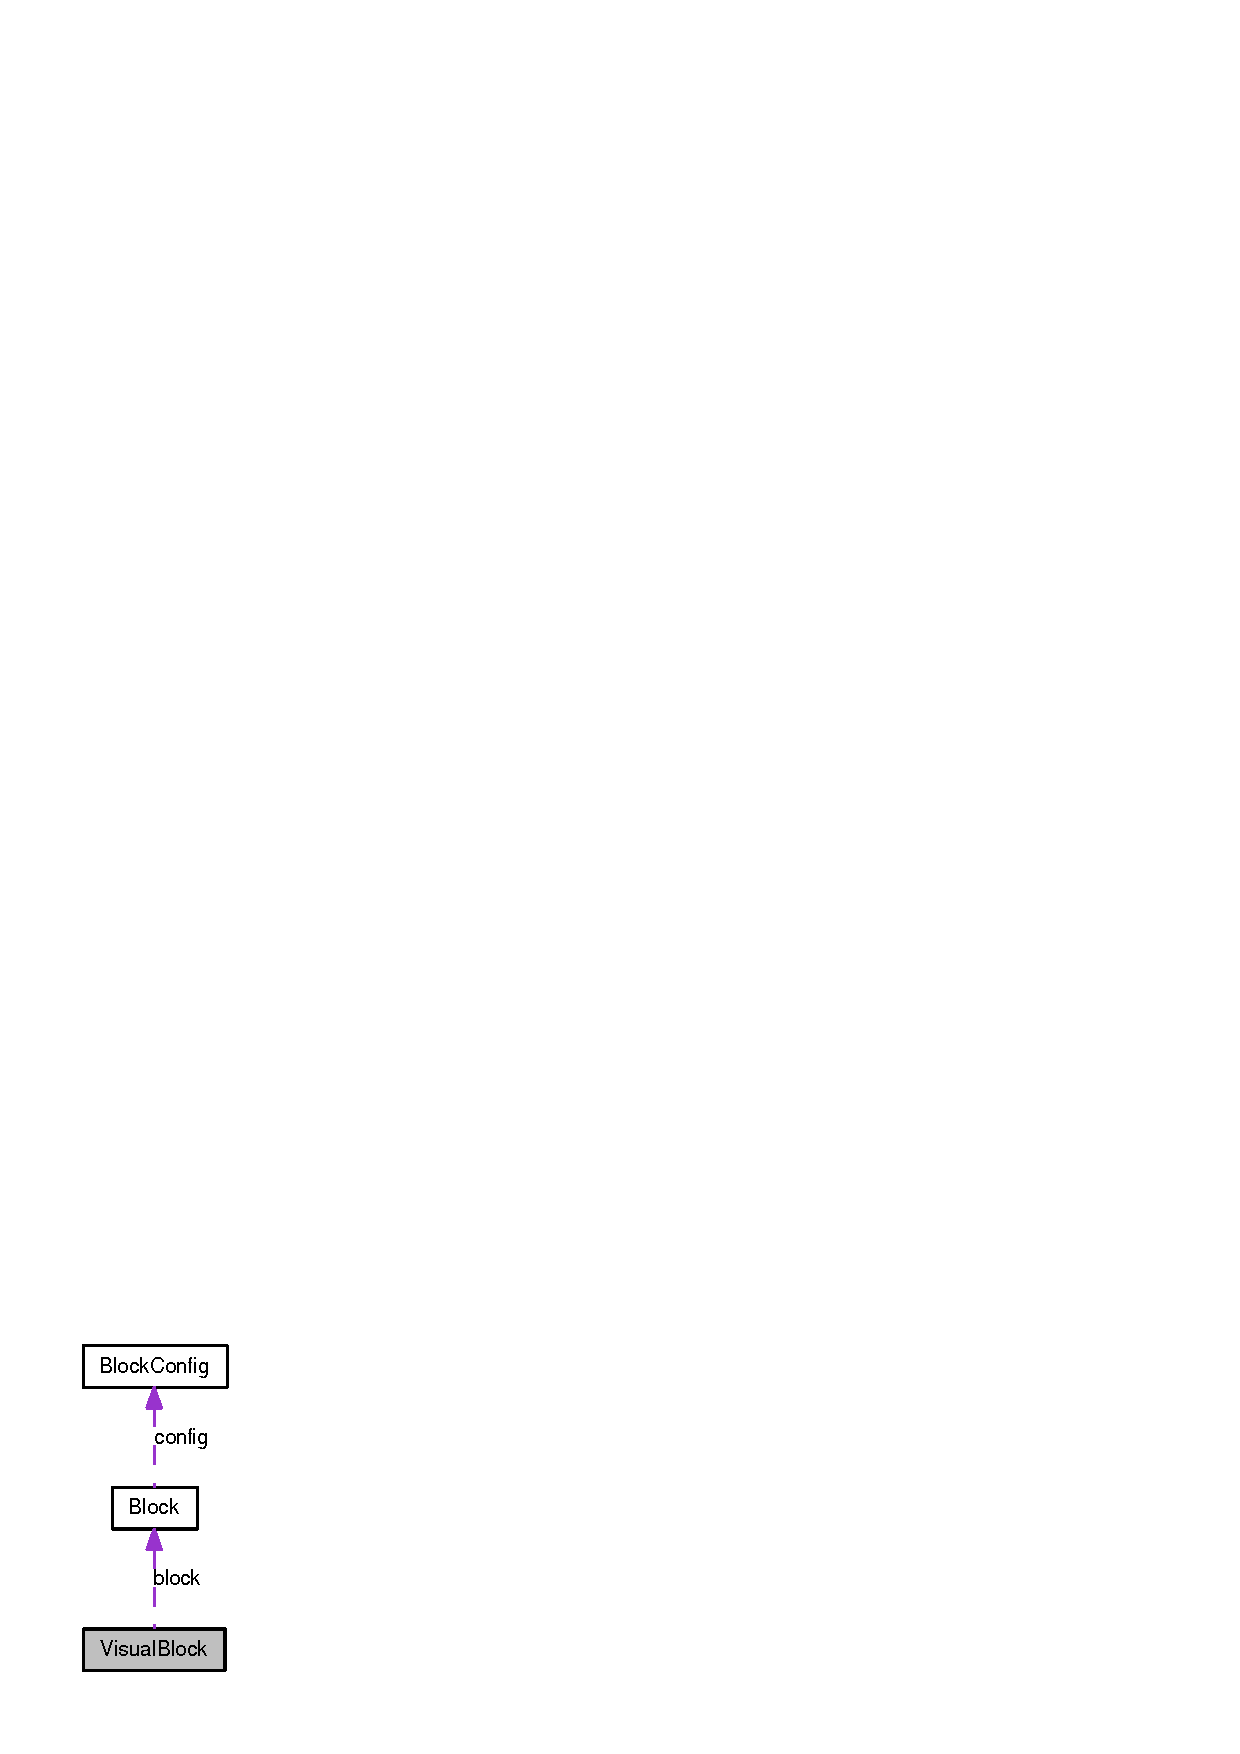
\includegraphics[width=56pt]{classVisualBlock__coll__graph}
\end{center}
\end{figure}
\subsection*{Public Member Functions}
\begin{CompactItemize}
\item 
\_\-\_\-fastcall \hyperlink{classVisualBlock_19ba01bbc2f90d861528bf705b93aa05}{VisualBlock} (TComponent $\ast$Owner)
\item 
\_\-\_\-fastcall \hyperlink{classVisualBlock_88dac1befb8f8aa9d3435c8c35d1ffee}{$\sim$VisualBlock} ()
\item 
\hyperlink{structPosition}{Position} \hyperlink{classVisualBlock_f4bfdf59b184dd79ceaacb57f9acfd66}{getInputPosition} (\hyperlink{classBlockInput}{BlockInput} $\ast$object)
\item 
\hyperlink{structPosition}{Position} \hyperlink{classVisualBlock_840c712434dddf714a3cee9200073114}{getOutputPosition} (\hyperlink{classBlockOutput}{BlockOutput} $\ast$object)
\item 
bool \hyperlink{classVisualBlock_c7db3e3d6aabc762ea055453855c7448}{setConfigButtonGlyph} (Graphics::TBitmap $\ast$bmp)
\item 
void \hyperlink{classVisualBlock_62361923d36c7162a2ce8919e4f0949f}{setTitle} (const AnsiString \&s)
\item 
AnsiString \hyperlink{classVisualBlock_a7581d6b296ce3069bd7e16438fd330e}{getTitle} ()
\item 
bool \hyperlink{classVisualBlock_c484b8959917ac7901aad3ac60740b0d}{updateVisualComponents} ()
\item 
bool \hyperlink{classVisualBlock_22d016593be16c1d77e19c9a42d80afe}{updateHistory} ()
\item 
void \hyperlink{classVisualBlock_8ca3f7d1dcc59e9383df931ed57a76c1}{setSelected} (bool \hyperlink{classVisualBlock_848de7730beb758d3c427f99ab78deaf}{status})
\item 
bool \hyperlink{classVisualBlock_046a93138fb3800d114e176ab9e4c164}{isSelected} ()
\item 
void \hyperlink{classVisualBlock_849044a8c705427b0bce5a6808e53115}{setStatusColor} (TColor cl)
\end{CompactItemize}
\subsection*{Public Attributes}
\begin{CompactItemize}
\item 
\hyperlink{classBlock}{Block} \hyperlink{classVisualBlock_76bfcfa68286004c352c4736635be0cb}{block}
\item 
AnsiString \hyperlink{classVisualBlock_08efb43e1546631cb54848002d809a23}{nameOfBlock}
\item 
int \hyperlink{classVisualBlock_726797ae619bdd874806321c7b878607}{numberOfBlock}
\item 
bool \hyperlink{classVisualBlock_3bc0c90322c4b39a85de000a2d036413}{runned}
\item 
\hyperlink{BlockHistory_8h_1e80e0966c4a2e68a83338258a89f5ae}{vectorBlockHistory} \hyperlink{classVisualBlock_bae4197cd71315bf74e26e9e7f04bc8c}{history}
\item 
vector$<$ \hyperlink{classVisualInput}{VisualInput} $\ast$ $>$ \hyperlink{classVisualBlock_8f4a1e25447f63dd82fef4ca1b5fa036}{leftInput}
\item 
vector$<$ \hyperlink{classVisualInput}{VisualInput} $\ast$ $>$ \hyperlink{classVisualBlock_ea0803cef47e1cd7f3c3fd92268b2d5c}{topInput}
\item 
vector$<$ \hyperlink{classVisualOutput}{VisualOutput} $\ast$ $>$ \hyperlink{classVisualBlock_e87bdb704a2ac4af6bc51b34456fdd1d}{rightOutput}
\item 
vector$<$ \hyperlink{classVisualOutput}{VisualOutput} $\ast$ $>$ \hyperlink{classVisualBlock_c20150edf6b145056e52ef811d3e977a}{bottomOutput}
\item 
VisualFunction \hyperlink{classVisualBlock_b342e90eddc48bc614d0a9da48f0e7e4}{OnConfigClick}
\item 
VisualBlock\_\-FunctionI \hyperlink{classVisualBlock_8fc6c9338da4af652d7d1fe170754f7b}{OnVisualInputSelected}
\item 
VisualBlock\_\-FunctionO \hyperlink{classVisualBlock_2c6a85164bf488a2b1055be8331aa813}{OnVisualOutputSelected}
\item 
VisualBlock\_\-FunctionHI \hyperlink{classVisualBlock_aa5ecd1d9c57caa0a9b08ece183dc9da}{OnVInputHistory}
\item 
VisualBlock\_\-FunctionHO \hyperlink{classVisualBlock_9a624de525f52a202cd57062f42332f3}{OnVOutputHistory}
\item 
VisualBlock\_\-FunctionMove \hyperlink{classVisualBlock_a01dc407b0ccc5d72e4ba2b3cc67bbc0}{OnBlockMove}
\item 
VisualFunction \hyperlink{classVisualBlock_10238a1e11bc16de548c0e0ae7118ccf}{OnUnselect}
\item 
VisualFunction \hyperlink{classVisualBlock_425f00a0257fc0f25e01b8e4eb24f3f7}{OnSelect}
\item 
VisualFunction \hyperlink{classVisualBlock_9398455ed1a288276ddc1845cd409d9f}{OnSelectAdd}
\end{CompactItemize}
\subsection*{Private Member Functions}
\begin{CompactItemize}
\item 
void \_\-\_\-fastcall \hyperlink{classVisualBlock_12b120084c71ac8e29f8b527401e9bb6}{SpeedButtonClick} (TObject $\ast$Sender)
\item 
void \_\-\_\-fastcall \hyperlink{classVisualBlock_a6eb1b3dcbbbb50d21bfb263935c6780}{InputSelected} (TObject $\ast$Sender)
\item 
void \_\-\_\-fastcall \hyperlink{classVisualBlock_79906715a0a58e622284b4be0402d13d}{OutputSelected} (TObject $\ast$Sender)
\item 
void \hyperlink{classVisualBlock_0dd05c49185b9c4ed3c2067c2887207c}{InputShowHistory} (TObject $\ast$Sender)
\item 
void \hyperlink{classVisualBlock_a06f4f819f1ffb8210552be1b2588241}{OutputShowHistory} (TObject $\ast$Sender)
\item 
void \_\-\_\-fastcall \hyperlink{classVisualBlock_92cda5ed352c37bdf35821d733a9eec0}{BlockClick} (TObject $\ast$Sender)
\item 
void \_\-\_\-fastcall \hyperlink{classVisualBlock_4105b606e41f9682f565a982e5ba78ac}{BlockMouseDown} (TObject $\ast$Sender, TMouseButton Button, TShiftState Shift, int X, int Y)
\item 
void \_\-\_\-fastcall \hyperlink{classVisualBlock_e4aaf7841bf53a143a3c83df422dc387}{BlockMouseUp} (TObject $\ast$Sender, TMouseButton Button, TShiftState Shift, int X, int Y)
\item 
void \_\-\_\-fastcall \hyperlink{classVisualBlock_f88b17e4ee367aa1bd52e0ba403e3ec9}{BlockMouseMove} (TObject $\ast$Sender, TShiftState Shift, int X, int Y)
\item 
void \hyperlink{classVisualBlock_120c84328c3017aec8fc669d156883a6}{resizeAll} ()
\end{CompactItemize}
\subsection*{Private Attributes}
\begin{CompactItemize}
\item 
TSpeedButton $\ast$ \hyperlink{classVisualBlock_12c5a7d37bad2fe96c1e681193e46692}{configButton}
\item 
TLabel $\ast$ \hyperlink{classVisualBlock_fb8a08d0bdaabd2f2c9331c73b327e94}{title}
\item 
TPanel $\ast$ \hyperlink{classVisualBlock_848de7730beb758d3c427f99ab78deaf}{status}
\item 
bool \hyperlink{classVisualBlock_6d94e21639a7e021c92a0fd31e859487}{selected}
\item 
bool \hyperlink{classVisualBlock_e8a5a106bf510e7029c0f453e6ecd999}{moving}
\item 
bool \hyperlink{classVisualBlock_b3035554398e30e608325b6c640ace2d}{button}
\item 
TPoint \hyperlink{classVisualBlock_43953361a9b50884f92ed3e9ee90c5b2}{oldPoint}
\end{CompactItemize}


\subsection{Detailed Description}
Klasa wyswietla caly bloczek 

Definition at line 30 of file VisualBlock.h.

\subsection{Constructor \& Destructor Documentation}
\hypertarget{classVisualBlock_19ba01bbc2f90d861528bf705b93aa05}{
\index{VisualBlock@{VisualBlock}!VisualBlock@{VisualBlock}}
\index{VisualBlock@{VisualBlock}!VisualBlock@{VisualBlock}}
\subsubsection[VisualBlock]{\setlength{\rightskip}{0pt plus 5cm}\_\-\_\-fastcall VisualBlock::VisualBlock (TComponent $\ast$ {\em Owner})}}
\label{classVisualBlock_19ba01bbc2f90d861528bf705b93aa05}


Konstruktor \begin{Desc}
\item[Parameters:]
\begin{description}
\item[{\em Owner}]klasa nadrzedna dla tej klasy \end{description}
\end{Desc}


Definition at line 6 of file VisualBlock.cpp.

References BlockClick(), BlockMouseDown(), BlockMouseMove(), BlockMouseUp(), configButton, moving, nameOfBlock, numberOfBlock, OnBlockMove, OnSelect, OnSelectAdd, OnUnselect, OnVInputHistory, OnVisualInputSelected, OnVisualOutputSelected, OnVOutputHistory, runned, selected, SpeedButtonClick(), status, and title.\hypertarget{classVisualBlock_88dac1befb8f8aa9d3435c8c35d1ffee}{
\index{VisualBlock@{VisualBlock}!$\sim$VisualBlock@{$\sim$VisualBlock}}
\index{$\sim$VisualBlock@{$\sim$VisualBlock}!VisualBlock@{VisualBlock}}
\subsubsection[$\sim$VisualBlock]{\setlength{\rightskip}{0pt plus 5cm}\_\-\_\-fastcall VisualBlock::$\sim$VisualBlock ()}}
\label{classVisualBlock_88dac1befb8f8aa9d3435c8c35d1ffee}


Destruktor 

Definition at line 85 of file VisualBlock.cpp.

References bottomOutput, configButton, history, leftInput, rightOutput, status, title, and topInput.

\subsection{Member Function Documentation}
\hypertarget{classVisualBlock_12b120084c71ac8e29f8b527401e9bb6}{
\index{VisualBlock@{VisualBlock}!SpeedButtonClick@{SpeedButtonClick}}
\index{SpeedButtonClick@{SpeedButtonClick}!VisualBlock@{VisualBlock}}
\subsubsection[SpeedButtonClick]{\setlength{\rightskip}{0pt plus 5cm}void \_\-\_\-fastcall VisualBlock::SpeedButtonClick (TObject $\ast$ {\em Sender})\hspace{0.3cm}{\tt  \mbox{[}private\mbox{]}}}}
\label{classVisualBlock_12b120084c71ac8e29f8b527401e9bb6}




Definition at line 190 of file VisualBlock.cpp.

References OnConfigClick.

Referenced by VisualBlock().\hypertarget{classVisualBlock_a6eb1b3dcbbbb50d21bfb263935c6780}{
\index{VisualBlock@{VisualBlock}!InputSelected@{InputSelected}}
\index{InputSelected@{InputSelected}!VisualBlock@{VisualBlock}}
\subsubsection[InputSelected]{\setlength{\rightskip}{0pt plus 5cm}void \_\-\_\-fastcall VisualBlock::InputSelected (TObject $\ast$ {\em Sender})\hspace{0.3cm}{\tt  \mbox{[}private\mbox{]}}}}
\label{classVisualBlock_a6eb1b3dcbbbb50d21bfb263935c6780}




Definition at line 487 of file VisualBlock.cpp.

References OnVisualInputSelected.

Referenced by updateVisualComponents().\hypertarget{classVisualBlock_79906715a0a58e622284b4be0402d13d}{
\index{VisualBlock@{VisualBlock}!OutputSelected@{OutputSelected}}
\index{OutputSelected@{OutputSelected}!VisualBlock@{VisualBlock}}
\subsubsection[OutputSelected]{\setlength{\rightskip}{0pt plus 5cm}void \_\-\_\-fastcall VisualBlock::OutputSelected (TObject $\ast$ {\em Sender})\hspace{0.3cm}{\tt  \mbox{[}private\mbox{]}}}}
\label{classVisualBlock_79906715a0a58e622284b4be0402d13d}




Definition at line 493 of file VisualBlock.cpp.

References OnVisualOutputSelected.

Referenced by updateVisualComponents().\hypertarget{classVisualBlock_0dd05c49185b9c4ed3c2067c2887207c}{
\index{VisualBlock@{VisualBlock}!InputShowHistory@{InputShowHistory}}
\index{InputShowHistory@{InputShowHistory}!VisualBlock@{VisualBlock}}
\subsubsection[InputShowHistory]{\setlength{\rightskip}{0pt plus 5cm}void VisualBlock::InputShowHistory (TObject $\ast$ {\em Sender})\hspace{0.3cm}{\tt  \mbox{[}private\mbox{]}}}}
\label{classVisualBlock_0dd05c49185b9c4ed3c2067c2887207c}




Definition at line 499 of file VisualBlock.cpp.

References OnVInputHistory.

Referenced by updateVisualComponents().\hypertarget{classVisualBlock_a06f4f819f1ffb8210552be1b2588241}{
\index{VisualBlock@{VisualBlock}!OutputShowHistory@{OutputShowHistory}}
\index{OutputShowHistory@{OutputShowHistory}!VisualBlock@{VisualBlock}}
\subsubsection[OutputShowHistory]{\setlength{\rightskip}{0pt plus 5cm}void VisualBlock::OutputShowHistory (TObject $\ast$ {\em Sender})\hspace{0.3cm}{\tt  \mbox{[}private\mbox{]}}}}
\label{classVisualBlock_a06f4f819f1ffb8210552be1b2588241}




Definition at line 505 of file VisualBlock.cpp.

References OnVOutputHistory.

Referenced by updateVisualComponents().\hypertarget{classVisualBlock_92cda5ed352c37bdf35821d733a9eec0}{
\index{VisualBlock@{VisualBlock}!BlockClick@{BlockClick}}
\index{BlockClick@{BlockClick}!VisualBlock@{VisualBlock}}
\subsubsection[BlockClick]{\setlength{\rightskip}{0pt plus 5cm}void \_\-\_\-fastcall VisualBlock::BlockClick (TObject $\ast$ {\em Sender})\hspace{0.3cm}{\tt  \mbox{[}private\mbox{]}}}}
\label{classVisualBlock_92cda5ed352c37bdf35821d733a9eec0}




Definition at line 529 of file VisualBlock.cpp.

References altDown(), ctrlDown(), moving, OnSelect, OnSelectAdd, OnUnselect, selected, and setSelected().

Referenced by VisualBlock().\hypertarget{classVisualBlock_4105b606e41f9682f565a982e5ba78ac}{
\index{VisualBlock@{VisualBlock}!BlockMouseDown@{BlockMouseDown}}
\index{BlockMouseDown@{BlockMouseDown}!VisualBlock@{VisualBlock}}
\subsubsection[BlockMouseDown]{\setlength{\rightskip}{0pt plus 5cm}void \_\-\_\-fastcall VisualBlock::BlockMouseDown (TObject $\ast$ {\em Sender}, \/  TMouseButton {\em Button}, \/  TShiftState {\em Shift}, \/  int {\em X}, \/  int {\em Y})\hspace{0.3cm}{\tt  \mbox{[}private\mbox{]}}}}
\label{classVisualBlock_4105b606e41f9682f565a982e5ba78ac}




Definition at line 554 of file VisualBlock.cpp.

References BlockMouseMove(), BlockMouseUp(), button, moving, oldPoint, OnSelect, OnSelectAdd, PIWOMAINCLASSTYPE, selected, and setSelected().

Referenced by VisualBlock().\hypertarget{classVisualBlock_e4aaf7841bf53a143a3c83df422dc387}{
\index{VisualBlock@{VisualBlock}!BlockMouseUp@{BlockMouseUp}}
\index{BlockMouseUp@{BlockMouseUp}!VisualBlock@{VisualBlock}}
\subsubsection[BlockMouseUp]{\setlength{\rightskip}{0pt plus 5cm}void \_\-\_\-fastcall VisualBlock::BlockMouseUp (TObject $\ast$ {\em Sender}, \/  TMouseButton {\em Button}, \/  TShiftState {\em Shift}, \/  int {\em X}, \/  int {\em Y})\hspace{0.3cm}{\tt  \mbox{[}private\mbox{]}}}}
\label{classVisualBlock_e4aaf7841bf53a143a3c83df422dc387}




Definition at line 601 of file VisualBlock.cpp.

References moving, and PIWOMAINCLASSTYPE.

Referenced by BlockMouseDown(), and VisualBlock().\hypertarget{classVisualBlock_f88b17e4ee367aa1bd52e0ba403e3ec9}{
\index{VisualBlock@{VisualBlock}!BlockMouseMove@{BlockMouseMove}}
\index{BlockMouseMove@{BlockMouseMove}!VisualBlock@{VisualBlock}}
\subsubsection[BlockMouseMove]{\setlength{\rightskip}{0pt plus 5cm}void \_\-\_\-fastcall VisualBlock::BlockMouseMove (TObject $\ast$ {\em Sender}, \/  TShiftState {\em Shift}, \/  int {\em X}, \/  int {\em Y})\hspace{0.3cm}{\tt  \mbox{[}private\mbox{]}}}}
\label{classVisualBlock_f88b17e4ee367aa1bd52e0ba403e3ec9}




Definition at line 609 of file VisualBlock.cpp.

References button, moving, oldPoint, and OnBlockMove.

Referenced by BlockMouseDown(), and VisualBlock().\hypertarget{classVisualBlock_120c84328c3017aec8fc669d156883a6}{
\index{VisualBlock@{VisualBlock}!resizeAll@{resizeAll}}
\index{resizeAll@{resizeAll}!VisualBlock@{VisualBlock}}
\subsubsection[resizeAll]{\setlength{\rightskip}{0pt plus 5cm}void VisualBlock::resizeAll ()\hspace{0.3cm}{\tt  \mbox{[}private\mbox{]}}}}
\label{classVisualBlock_120c84328c3017aec8fc669d156883a6}




Definition at line 411 of file VisualBlock.cpp.

References bottomOutput, leftInput, rightOutput, status, title, and topInput.

Referenced by updateVisualComponents().\hypertarget{classVisualBlock_f4bfdf59b184dd79ceaacb57f9acfd66}{
\index{VisualBlock@{VisualBlock}!getInputPosition@{getInputPosition}}
\index{getInputPosition@{getInputPosition}!VisualBlock@{VisualBlock}}
\subsubsection[getInputPosition]{\setlength{\rightskip}{0pt plus 5cm}{\bf Position} VisualBlock::getInputPosition ({\bf BlockInput} $\ast$ {\em object})}}
\label{classVisualBlock_f4bfdf59b184dd79ceaacb57f9acfd66}


Pobiera pozycje wejscia do bloku \begin{Desc}
\item[Parameters:]
\begin{description}
\item[{\em object}]wejscie \end{description}
\end{Desc}
\begin{Desc}
\item[Returns:]pozycja \end{Desc}


Definition at line 122 of file VisualBlock.cpp.

References Position::direction, leftInput, topInput, and Position::xy.

Referenced by Connection::connectionOk(), and Connection::draw().\hypertarget{classVisualBlock_840c712434dddf714a3cee9200073114}{
\index{VisualBlock@{VisualBlock}!getOutputPosition@{getOutputPosition}}
\index{getOutputPosition@{getOutputPosition}!VisualBlock@{VisualBlock}}
\subsubsection[getOutputPosition]{\setlength{\rightskip}{0pt plus 5cm}{\bf Position} VisualBlock::getOutputPosition ({\bf BlockOutput} $\ast$ {\em object})}}
\label{classVisualBlock_840c712434dddf714a3cee9200073114}


Pobiera pozycje wyjscia z bloku \begin{Desc}
\item[Parameters:]
\begin{description}
\item[{\em object}]wyjscia \end{description}
\end{Desc}
\begin{Desc}
\item[Returns:]pozycja \end{Desc}


Definition at line 156 of file VisualBlock.cpp.

References bottomOutput, Position::direction, rightOutput, and Position::xy.

Referenced by Connection::connectionOk(), and Connection::draw().\hypertarget{classVisualBlock_c7db3e3d6aabc762ea055453855c7448}{
\index{VisualBlock@{VisualBlock}!setConfigButtonGlyph@{setConfigButtonGlyph}}
\index{setConfigButtonGlyph@{setConfigButtonGlyph}!VisualBlock@{VisualBlock}}
\subsubsection[setConfigButtonGlyph]{\setlength{\rightskip}{0pt plus 5cm}bool VisualBlock::setConfigButtonGlyph (Graphics::TBitmap $\ast$ {\em bmp})}}
\label{classVisualBlock_c7db3e3d6aabc762ea055453855c7448}


Ustawia nowy obrazek jako obrazek pokazujacy sie na przycusku konfiguracyjnym \begin{Desc}
\item[Parameters:]
\begin{description}
\item[{\em bmp}]obrazek \end{description}
\end{Desc}
\begin{Desc}
\item[Returns:]true jesli operacja sie powiodla \end{Desc}


Definition at line 197 of file VisualBlock.cpp.

References configButton.

Referenced by PIWOEngine::AddBlock(), PIWOEngine::DuplcateSelectedBlocks(), and PIWOEngine::loadFromFile().\hypertarget{classVisualBlock_62361923d36c7162a2ce8919e4f0949f}{
\index{VisualBlock@{VisualBlock}!setTitle@{setTitle}}
\index{setTitle@{setTitle}!VisualBlock@{VisualBlock}}
\subsubsection[setTitle]{\setlength{\rightskip}{0pt plus 5cm}void VisualBlock::setTitle (const AnsiString \& {\em s})}}
\label{classVisualBlock_62361923d36c7162a2ce8919e4f0949f}


Ustawia tytul bloczka \begin{Desc}
\item[Parameters:]
\begin{description}
\item[{\em s}]nowy tytul \end{description}
\end{Desc}


Definition at line 204 of file VisualBlock.cpp.

References block, Block::title, and title.

Referenced by PIWOEngine::AddBlock(), PIWOEngine::DuplcateSelectedBlocks(), and PIWOEngine::loadFromFile().\hypertarget{classVisualBlock_a7581d6b296ce3069bd7e16438fd330e}{
\index{VisualBlock@{VisualBlock}!getTitle@{getTitle}}
\index{getTitle@{getTitle}!VisualBlock@{VisualBlock}}
\subsubsection[getTitle]{\setlength{\rightskip}{0pt plus 5cm}AnsiString VisualBlock::getTitle ()}}
\label{classVisualBlock_a7581d6b296ce3069bd7e16438fd330e}


Pobiera aktualny tytul bloczka \begin{Desc}
\item[Returns:]tytul \end{Desc}


Definition at line 211 of file VisualBlock.cpp.

References title.

Referenced by PIWOEngine::CancelCustomizationOnSelectedConnections(), PIWOEngine::DeleteSelectedConnection(), PIWOEngine::loadFromFile(), PIWOEngine::MakeConnection(), PIWOEngine::OnConnectionSelect(), PIWOEngine::OnVisualBlockConfigClick(), PIWOEngine::OnVisualBlockInputHistoryClick(), PIWOEngine::OnVisualBlockInputSelected(), PIWOEngine::OnVisualBlockOutputHistoryClick(), PIWOEngine::OnVisualBlockOutputSelected(), PIWOEngine::OnVisualBlockUnselect(), THistory::refresh(), PIWOEngine::runBlock(), PIWOEngine::UnselectSelectedConnection(), Connection::update(), and PIWOEngine::validateBlock().\hypertarget{classVisualBlock_c484b8959917ac7901aad3ac60740b0d}{
\index{VisualBlock@{VisualBlock}!updateVisualComponents@{updateVisualComponents}}
\index{updateVisualComponents@{updateVisualComponents}!VisualBlock@{VisualBlock}}
\subsubsection[updateVisualComponents]{\setlength{\rightskip}{0pt plus 5cm}bool VisualBlock::updateVisualComponents ()}}
\label{classVisualBlock_c484b8959917ac7901aad3ac60740b0d}


Dostosowuje wizualne infomacje o bloczku do informacji zawartych w niskopoziomowej klasie \hyperlink{classBlock}{Block}. \begin{Desc}
\item[Returns:]false gdy wystapil blad \end{Desc}


Definition at line 216 of file VisualBlock.cpp.

References BlockInput::allowedTypes, block, configButton, BlockInput::getConnectedType(), BlockElement::getDescription(), BlockElement::getErrorCode(), BlockElement::getErrorDescription(), BlockOutput::getOutputType(), VisualInput::input, Block::input, InputSelected(), InputShowHistory(), leftInput, VisualInputOutput::OnShowHistory, VisualOutput::output, Block::output, OutputSelected(), OutputShowHistory(), resizeAll(), rightOutput, status, and title.

Referenced by PIWOEngine::AddBlock(), PIWOEngine::DuplcateSelectedBlocks(), PIWOEngine::loadFromFile(), PIWOEngine::runBlock(), and PIWOEngine::validateBlock().\hypertarget{classVisualBlock_22d016593be16c1d77e19c9a42d80afe}{
\index{VisualBlock@{VisualBlock}!updateHistory@{updateHistory}}
\index{updateHistory@{updateHistory}!VisualBlock@{VisualBlock}}
\subsubsection[updateHistory]{\setlength{\rightskip}{0pt plus 5cm}bool VisualBlock::updateHistory ()}}
\label{classVisualBlock_22d016593be16c1d77e19c9a42d80afe}


Aktualizuje historie usuwajac z niej wszelkie przedawnione i nieaktualne dane 

Definition at line 365 of file VisualBlock.cpp.

References block, bottomOutput, Block::getConfig(), BlockConfig::getRevision(), history, leftInput, rightOutput, and topInput.

Referenced by PIWOEngine::validateBlock().\hypertarget{classVisualBlock_8ca3f7d1dcc59e9383df931ed57a76c1}{
\index{VisualBlock@{VisualBlock}!setSelected@{setSelected}}
\index{setSelected@{setSelected}!VisualBlock@{VisualBlock}}
\subsubsection[setSelected]{\setlength{\rightskip}{0pt plus 5cm}void VisualBlock::setSelected (bool {\em status})}}
\label{classVisualBlock_8ca3f7d1dcc59e9383df931ed57a76c1}


Zaznacza/Odznacza blok \begin{Desc}
\item[Parameters:]
\begin{description}
\item[{\em status}]true -zaznaczony, false - odznaczony \end{description}
\end{Desc}


Definition at line 511 of file VisualBlock.cpp.

References selected.

Referenced by PIWOEngine::AddBlock(), BlockClick(), BlockMouseDown(), and PIWOEngine::OnVisualBlockUnselect().\hypertarget{classVisualBlock_046a93138fb3800d114e176ab9e4c164}{
\index{VisualBlock@{VisualBlock}!isSelected@{isSelected}}
\index{isSelected@{isSelected}!VisualBlock@{VisualBlock}}
\subsubsection[isSelected]{\setlength{\rightskip}{0pt plus 5cm}bool VisualBlock::isSelected ()}}
\label{classVisualBlock_046a93138fb3800d114e176ab9e4c164}


Informuje o tym czy blok jest juz zaznaczony \begin{Desc}
\item[Returns:]true - zaznaczony, false - nie zaznaczony \end{Desc}


Definition at line 524 of file VisualBlock.cpp.

References selected.\hypertarget{classVisualBlock_849044a8c705427b0bce5a6808e53115}{
\index{VisualBlock@{VisualBlock}!setStatusColor@{setStatusColor}}
\index{setStatusColor@{setStatusColor}!VisualBlock@{VisualBlock}}
\subsubsection[setStatusColor]{\setlength{\rightskip}{0pt plus 5cm}void VisualBlock::setStatusColor (TColor {\em cl})}}
\label{classVisualBlock_849044a8c705427b0bce5a6808e53115}


Ustawia kolor statusu bloczka - widniejacy do okola przycisku konfiguracyjnego \begin{Desc}
\item[Parameters:]
\begin{description}
\item[{\em cl}]nowy kolor \end{description}
\end{Desc}


Definition at line 639 of file VisualBlock.cpp.

References status.

Referenced by PIWOEngine::runBlock().

\subsection{Member Data Documentation}
\hypertarget{classVisualBlock_12c5a7d37bad2fe96c1e681193e46692}{
\index{VisualBlock@{VisualBlock}!configButton@{configButton}}
\index{configButton@{configButton}!VisualBlock@{VisualBlock}}
\subsubsection[configButton]{\setlength{\rightskip}{0pt plus 5cm}TSpeedButton$\ast$ {\bf VisualBlock::configButton}\hspace{0.3cm}{\tt  \mbox{[}private\mbox{]}}}}
\label{classVisualBlock_12c5a7d37bad2fe96c1e681193e46692}




Definition at line 33 of file VisualBlock.h.

Referenced by setConfigButtonGlyph(), updateVisualComponents(), VisualBlock(), and $\sim$VisualBlock().\hypertarget{classVisualBlock_fb8a08d0bdaabd2f2c9331c73b327e94}{
\index{VisualBlock@{VisualBlock}!title@{title}}
\index{title@{title}!VisualBlock@{VisualBlock}}
\subsubsection[title]{\setlength{\rightskip}{0pt plus 5cm}TLabel$\ast$ {\bf VisualBlock::title}\hspace{0.3cm}{\tt  \mbox{[}private\mbox{]}}}}
\label{classVisualBlock_fb8a08d0bdaabd2f2c9331c73b327e94}




Definition at line 34 of file VisualBlock.h.

Referenced by getTitle(), resizeAll(), setTitle(), updateVisualComponents(), VisualBlock(), and $\sim$VisualBlock().\hypertarget{classVisualBlock_848de7730beb758d3c427f99ab78deaf}{
\index{VisualBlock@{VisualBlock}!status@{status}}
\index{status@{status}!VisualBlock@{VisualBlock}}
\subsubsection[status]{\setlength{\rightskip}{0pt plus 5cm}TPanel$\ast$ {\bf VisualBlock::status}\hspace{0.3cm}{\tt  \mbox{[}private\mbox{]}}}}
\label{classVisualBlock_848de7730beb758d3c427f99ab78deaf}




Definition at line 35 of file VisualBlock.h.

Referenced by resizeAll(), setStatusColor(), updateVisualComponents(), VisualBlock(), and $\sim$VisualBlock().\hypertarget{classVisualBlock_6d94e21639a7e021c92a0fd31e859487}{
\index{VisualBlock@{VisualBlock}!selected@{selected}}
\index{selected@{selected}!VisualBlock@{VisualBlock}}
\subsubsection[selected]{\setlength{\rightskip}{0pt plus 5cm}bool {\bf VisualBlock::selected}\hspace{0.3cm}{\tt  \mbox{[}private\mbox{]}}}}
\label{classVisualBlock_6d94e21639a7e021c92a0fd31e859487}




Definition at line 36 of file VisualBlock.h.

Referenced by BlockClick(), BlockMouseDown(), isSelected(), setSelected(), and VisualBlock().\hypertarget{classVisualBlock_e8a5a106bf510e7029c0f453e6ecd999}{
\index{VisualBlock@{VisualBlock}!moving@{moving}}
\index{moving@{moving}!VisualBlock@{VisualBlock}}
\subsubsection[moving]{\setlength{\rightskip}{0pt plus 5cm}bool {\bf VisualBlock::moving}\hspace{0.3cm}{\tt  \mbox{[}private\mbox{]}}}}
\label{classVisualBlock_e8a5a106bf510e7029c0f453e6ecd999}




Definition at line 37 of file VisualBlock.h.

Referenced by BlockClick(), BlockMouseDown(), BlockMouseMove(), BlockMouseUp(), and VisualBlock().\hypertarget{classVisualBlock_b3035554398e30e608325b6c640ace2d}{
\index{VisualBlock@{VisualBlock}!button@{button}}
\index{button@{button}!VisualBlock@{VisualBlock}}
\subsubsection[button]{\setlength{\rightskip}{0pt plus 5cm}bool {\bf VisualBlock::button}\hspace{0.3cm}{\tt  \mbox{[}private\mbox{]}}}}
\label{classVisualBlock_b3035554398e30e608325b6c640ace2d}




Definition at line 38 of file VisualBlock.h.

Referenced by BlockMouseDown(), and BlockMouseMove().\hypertarget{classVisualBlock_43953361a9b50884f92ed3e9ee90c5b2}{
\index{VisualBlock@{VisualBlock}!oldPoint@{oldPoint}}
\index{oldPoint@{oldPoint}!VisualBlock@{VisualBlock}}
\subsubsection[oldPoint]{\setlength{\rightskip}{0pt plus 5cm}TPoint {\bf VisualBlock::oldPoint}\hspace{0.3cm}{\tt  \mbox{[}private\mbox{]}}}}
\label{classVisualBlock_43953361a9b50884f92ed3e9ee90c5b2}




Definition at line 39 of file VisualBlock.h.

Referenced by BlockMouseDown(), and BlockMouseMove().\hypertarget{classVisualBlock_76bfcfa68286004c352c4736635be0cb}{
\index{VisualBlock@{VisualBlock}!block@{block}}
\index{block@{block}!VisualBlock@{VisualBlock}}
\subsubsection[block]{\setlength{\rightskip}{0pt plus 5cm}{\bf Block} {\bf VisualBlock::block}}}
\label{classVisualBlock_76bfcfa68286004c352c4736635be0cb}


Blok w wersji niskopoziomowej 

Definition at line 54 of file VisualBlock.h.

Referenced by PIWOEngine::AddBlock(), PIWOEngine::DuplcateSelectedBlocks(), PIWOEngine::loadFromFile(), PIWOEngine::OnVisualBlockConfigClick(), PIWOEngine::runBlock(), setTitle(), updateHistory(), updateVisualComponents(), and PIWOEngine::validateBlock().\hypertarget{classVisualBlock_08efb43e1546631cb54848002d809a23}{
\index{VisualBlock@{VisualBlock}!nameOfBlock@{nameOfBlock}}
\index{nameOfBlock@{nameOfBlock}!VisualBlock@{VisualBlock}}
\subsubsection[nameOfBlock]{\setlength{\rightskip}{0pt plus 5cm}AnsiString {\bf VisualBlock::nameOfBlock}}}
\label{classVisualBlock_08efb43e1546631cb54848002d809a23}




Definition at line 55 of file VisualBlock.h.

Referenced by PIWOEngine::AddBlock(), PIWOEngine::DuplcateSelectedBlocks(), PIWOEngine::loadFromFile(), PIWOEngine::OnVisualBlockConfigClick(), PIWOEngine::runBlock(), PIWOEngine::validateBlock(), and VisualBlock().\hypertarget{classVisualBlock_726797ae619bdd874806321c7b878607}{
\index{VisualBlock@{VisualBlock}!numberOfBlock@{numberOfBlock}}
\index{numberOfBlock@{numberOfBlock}!VisualBlock@{VisualBlock}}
\subsubsection[numberOfBlock]{\setlength{\rightskip}{0pt plus 5cm}int {\bf VisualBlock::numberOfBlock}}}
\label{classVisualBlock_726797ae619bdd874806321c7b878607}




Definition at line 56 of file VisualBlock.h.

Referenced by PIWOEngine::AddBlock(), PIWOEngine::DuplcateSelectedBlocks(), PIWOEngine::loadFromFile(), and VisualBlock().\hypertarget{classVisualBlock_3bc0c90322c4b39a85de000a2d036413}{
\index{VisualBlock@{VisualBlock}!runned@{runned}}
\index{runned@{runned}!VisualBlock@{VisualBlock}}
\subsubsection[runned]{\setlength{\rightskip}{0pt plus 5cm}bool {\bf VisualBlock::runned}}}
\label{classVisualBlock_3bc0c90322c4b39a85de000a2d036413}


Informacja o tym czy blok zostal juz uruchomiony - zmienna pomocnicza, wewnetrzna 

Definition at line 60 of file VisualBlock.h.

Referenced by PIWOEngine::runBlock(), and VisualBlock().\hypertarget{classVisualBlock_bae4197cd71315bf74e26e9e7f04bc8c}{
\index{VisualBlock@{VisualBlock}!history@{history}}
\index{history@{history}!VisualBlock@{VisualBlock}}
\subsubsection[history]{\setlength{\rightskip}{0pt plus 5cm}{\bf vectorBlockHistory} {\bf VisualBlock::history}}}
\label{classVisualBlock_bae4197cd71315bf74e26e9e7f04bc8c}


Historia bloku 

Definition at line 64 of file VisualBlock.h.

Referenced by PIWOEngine::OnVisualBlockInputHistoryClick(), PIWOEngine::OnVisualBlockOutputHistoryClick(), THistory::refresh(), PIWOEngine::runBlock(), updateHistory(), and $\sim$VisualBlock().\hypertarget{classVisualBlock_8f4a1e25447f63dd82fef4ca1b5fa036}{
\index{VisualBlock@{VisualBlock}!leftInput@{leftInput}}
\index{leftInput@{leftInput}!VisualBlock@{VisualBlock}}
\subsubsection[leftInput]{\setlength{\rightskip}{0pt plus 5cm}vector$<${\bf VisualInput}$\ast$$>$ {\bf VisualBlock::leftInput}}}
\label{classVisualBlock_8f4a1e25447f63dd82fef4ca1b5fa036}


Lista wejsc do bloku z lewej strony 

Definition at line 68 of file VisualBlock.h.

Referenced by getInputPosition(), resizeAll(), PIWOEngine::runBlock(), updateHistory(), updateVisualComponents(), and $\sim$VisualBlock().\hypertarget{classVisualBlock_ea0803cef47e1cd7f3c3fd92268b2d5c}{
\index{VisualBlock@{VisualBlock}!topInput@{topInput}}
\index{topInput@{topInput}!VisualBlock@{VisualBlock}}
\subsubsection[topInput]{\setlength{\rightskip}{0pt plus 5cm}vector$<${\bf VisualInput}$\ast$$>$ {\bf VisualBlock::topInput}}}
\label{classVisualBlock_ea0803cef47e1cd7f3c3fd92268b2d5c}


Lista wejsc do bloku z gornej strony 

Definition at line 72 of file VisualBlock.h.

Referenced by getInputPosition(), resizeAll(), PIWOEngine::runBlock(), updateHistory(), and $\sim$VisualBlock().\hypertarget{classVisualBlock_e87bdb704a2ac4af6bc51b34456fdd1d}{
\index{VisualBlock@{VisualBlock}!rightOutput@{rightOutput}}
\index{rightOutput@{rightOutput}!VisualBlock@{VisualBlock}}
\subsubsection[rightOutput]{\setlength{\rightskip}{0pt plus 5cm}vector$<${\bf VisualOutput}$\ast$$>$ {\bf VisualBlock::rightOutput}}}
\label{classVisualBlock_e87bdb704a2ac4af6bc51b34456fdd1d}


Lista wyjsc z bloku z prawej strony 

Definition at line 76 of file VisualBlock.h.

Referenced by getOutputPosition(), resizeAll(), PIWOEngine::runBlock(), updateHistory(), updateVisualComponents(), and $\sim$VisualBlock().\hypertarget{classVisualBlock_c20150edf6b145056e52ef811d3e977a}{
\index{VisualBlock@{VisualBlock}!bottomOutput@{bottomOutput}}
\index{bottomOutput@{bottomOutput}!VisualBlock@{VisualBlock}}
\subsubsection[bottomOutput]{\setlength{\rightskip}{0pt plus 5cm}vector$<${\bf VisualOutput}$\ast$$>$ {\bf VisualBlock::bottomOutput}}}
\label{classVisualBlock_c20150edf6b145056e52ef811d3e977a}


Lista wyjsc z bloku z dolnej strony 

Definition at line 80 of file VisualBlock.h.

Referenced by getOutputPosition(), resizeAll(), PIWOEngine::runBlock(), updateHistory(), and $\sim$VisualBlock().\hypertarget{classVisualBlock_b342e90eddc48bc614d0a9da48f0e7e4}{
\index{VisualBlock@{VisualBlock}!OnConfigClick@{OnConfigClick}}
\index{OnConfigClick@{OnConfigClick}!VisualBlock@{VisualBlock}}
\subsubsection[OnConfigClick]{\setlength{\rightskip}{0pt plus 5cm}VisualFunction {\bf VisualBlock::OnConfigClick}}}
\label{classVisualBlock_b342e90eddc48bc614d0a9da48f0e7e4}


Event: gdy kliknieto przycisk konfiguracyjny 

Definition at line 85 of file VisualBlock.h.

Referenced by PIWOEngine::AddBlock(), PIWOEngine::DuplcateSelectedBlocks(), PIWOEngine::loadFromFile(), and SpeedButtonClick().\hypertarget{classVisualBlock_8fc6c9338da4af652d7d1fe170754f7b}{
\index{VisualBlock@{VisualBlock}!OnVisualInputSelected@{OnVisualInputSelected}}
\index{OnVisualInputSelected@{OnVisualInputSelected}!VisualBlock@{VisualBlock}}
\subsubsection[OnVisualInputSelected]{\setlength{\rightskip}{0pt plus 5cm}VisualBlock\_\-FunctionI {\bf VisualBlock::OnVisualInputSelected}}}
\label{classVisualBlock_8fc6c9338da4af652d7d1fe170754f7b}


Event: gdy kliknieto na wejscie bloku 

Definition at line 89 of file VisualBlock.h.

Referenced by PIWOEngine::AddBlock(), PIWOEngine::DuplcateSelectedBlocks(), InputSelected(), PIWOEngine::loadFromFile(), and VisualBlock().\hypertarget{classVisualBlock_2c6a85164bf488a2b1055be8331aa813}{
\index{VisualBlock@{VisualBlock}!OnVisualOutputSelected@{OnVisualOutputSelected}}
\index{OnVisualOutputSelected@{OnVisualOutputSelected}!VisualBlock@{VisualBlock}}
\subsubsection[OnVisualOutputSelected]{\setlength{\rightskip}{0pt plus 5cm}VisualBlock\_\-FunctionO {\bf VisualBlock::OnVisualOutputSelected}}}
\label{classVisualBlock_2c6a85164bf488a2b1055be8331aa813}


Event: gdy kliknieto na wyjscie bloku 

Definition at line 93 of file VisualBlock.h.

Referenced by PIWOEngine::AddBlock(), PIWOEngine::DuplcateSelectedBlocks(), PIWOEngine::loadFromFile(), OutputSelected(), and VisualBlock().\hypertarget{classVisualBlock_aa5ecd1d9c57caa0a9b08ece183dc9da}{
\index{VisualBlock@{VisualBlock}!OnVInputHistory@{OnVInputHistory}}
\index{OnVInputHistory@{OnVInputHistory}!VisualBlock@{VisualBlock}}
\subsubsection[OnVInputHistory]{\setlength{\rightskip}{0pt plus 5cm}VisualBlock\_\-FunctionHI {\bf VisualBlock::OnVInputHistory}}}
\label{classVisualBlock_aa5ecd1d9c57caa0a9b08ece183dc9da}


Event: gdy kliknieto prawym przycuskiem na wejscie bloku 

Definition at line 97 of file VisualBlock.h.

Referenced by PIWOEngine::AddBlock(), PIWOEngine::DuplcateSelectedBlocks(), InputShowHistory(), PIWOEngine::loadFromFile(), and VisualBlock().\hypertarget{classVisualBlock_9a624de525f52a202cd57062f42332f3}{
\index{VisualBlock@{VisualBlock}!OnVOutputHistory@{OnVOutputHistory}}
\index{OnVOutputHistory@{OnVOutputHistory}!VisualBlock@{VisualBlock}}
\subsubsection[OnVOutputHistory]{\setlength{\rightskip}{0pt plus 5cm}VisualBlock\_\-FunctionHO {\bf VisualBlock::OnVOutputHistory}}}
\label{classVisualBlock_9a624de525f52a202cd57062f42332f3}


Event: gdy kliknieto prawym przyciskiem na wyjscie bloku 

Definition at line 101 of file VisualBlock.h.

Referenced by PIWOEngine::AddBlock(), PIWOEngine::DuplcateSelectedBlocks(), PIWOEngine::loadFromFile(), OutputShowHistory(), and VisualBlock().\hypertarget{classVisualBlock_a01dc407b0ccc5d72e4ba2b3cc67bbc0}{
\index{VisualBlock@{VisualBlock}!OnBlockMove@{OnBlockMove}}
\index{OnBlockMove@{OnBlockMove}!VisualBlock@{VisualBlock}}
\subsubsection[OnBlockMove]{\setlength{\rightskip}{0pt plus 5cm}VisualBlock\_\-FunctionMove {\bf VisualBlock::OnBlockMove}}}
\label{classVisualBlock_a01dc407b0ccc5d72e4ba2b3cc67bbc0}


Event: gdy przesunieto blok 

Definition at line 105 of file VisualBlock.h.

Referenced by PIWOEngine::AddBlock(), BlockMouseMove(), PIWOEngine::DuplcateSelectedBlocks(), PIWOEngine::loadFromFile(), and VisualBlock().\hypertarget{classVisualBlock_10238a1e11bc16de548c0e0ae7118ccf}{
\index{VisualBlock@{VisualBlock}!OnUnselect@{OnUnselect}}
\index{OnUnselect@{OnUnselect}!VisualBlock@{VisualBlock}}
\subsubsection[OnUnselect]{\setlength{\rightskip}{0pt plus 5cm}VisualFunction {\bf VisualBlock::OnUnselect}}}
\label{classVisualBlock_10238a1e11bc16de548c0e0ae7118ccf}


Event: gdy odznacozno blok 

Definition at line 109 of file VisualBlock.h.

Referenced by PIWOEngine::AddBlock(), BlockClick(), PIWOEngine::DuplcateSelectedBlocks(), PIWOEngine::loadFromFile(), and VisualBlock().\hypertarget{classVisualBlock_425f00a0257fc0f25e01b8e4eb24f3f7}{
\index{VisualBlock@{VisualBlock}!OnSelect@{OnSelect}}
\index{OnSelect@{OnSelect}!VisualBlock@{VisualBlock}}
\subsubsection[OnSelect]{\setlength{\rightskip}{0pt plus 5cm}VisualFunction {\bf VisualBlock::OnSelect}}}
\label{classVisualBlock_425f00a0257fc0f25e01b8e4eb24f3f7}


Event: gdy gdy zaznacozno blok, ale zarzadano odznaczenia innych 

Definition at line 113 of file VisualBlock.h.

Referenced by PIWOEngine::AddBlock(), BlockClick(), BlockMouseDown(), PIWOEngine::DuplcateSelectedBlocks(), PIWOEngine::loadFromFile(), and VisualBlock().\hypertarget{classVisualBlock_9398455ed1a288276ddc1845cd409d9f}{
\index{VisualBlock@{VisualBlock}!OnSelectAdd@{OnSelectAdd}}
\index{OnSelectAdd@{OnSelectAdd}!VisualBlock@{VisualBlock}}
\subsubsection[OnSelectAdd]{\setlength{\rightskip}{0pt plus 5cm}VisualFunction {\bf VisualBlock::OnSelectAdd}}}
\label{classVisualBlock_9398455ed1a288276ddc1845cd409d9f}


Event: gdy zaznaczono blok 

Definition at line 117 of file VisualBlock.h.

Referenced by PIWOEngine::AddBlock(), BlockClick(), BlockMouseDown(), PIWOEngine::DuplcateSelectedBlocks(), PIWOEngine::loadFromFile(), and VisualBlock().

The documentation for this class was generated from the following files:\begin{CompactItemize}
\item 
/PIWO/Program/gui/\hyperlink{VisualBlock_8h}{VisualBlock.h}\item 
/PIWO/Program/gui/\hyperlink{VisualBlock_8cpp}{VisualBlock.cpp}\end{CompactItemize}

\hypertarget{classVisualInput}{
\section{VisualInput Class Reference}
\label{classVisualInput}\index{VisualInput@{VisualInput}}
}
{\tt \#include $<$VisualInput.h$>$}

Inheritance diagram for VisualInput:\nopagebreak
\begin{figure}[H]
\begin{center}
\leavevmode
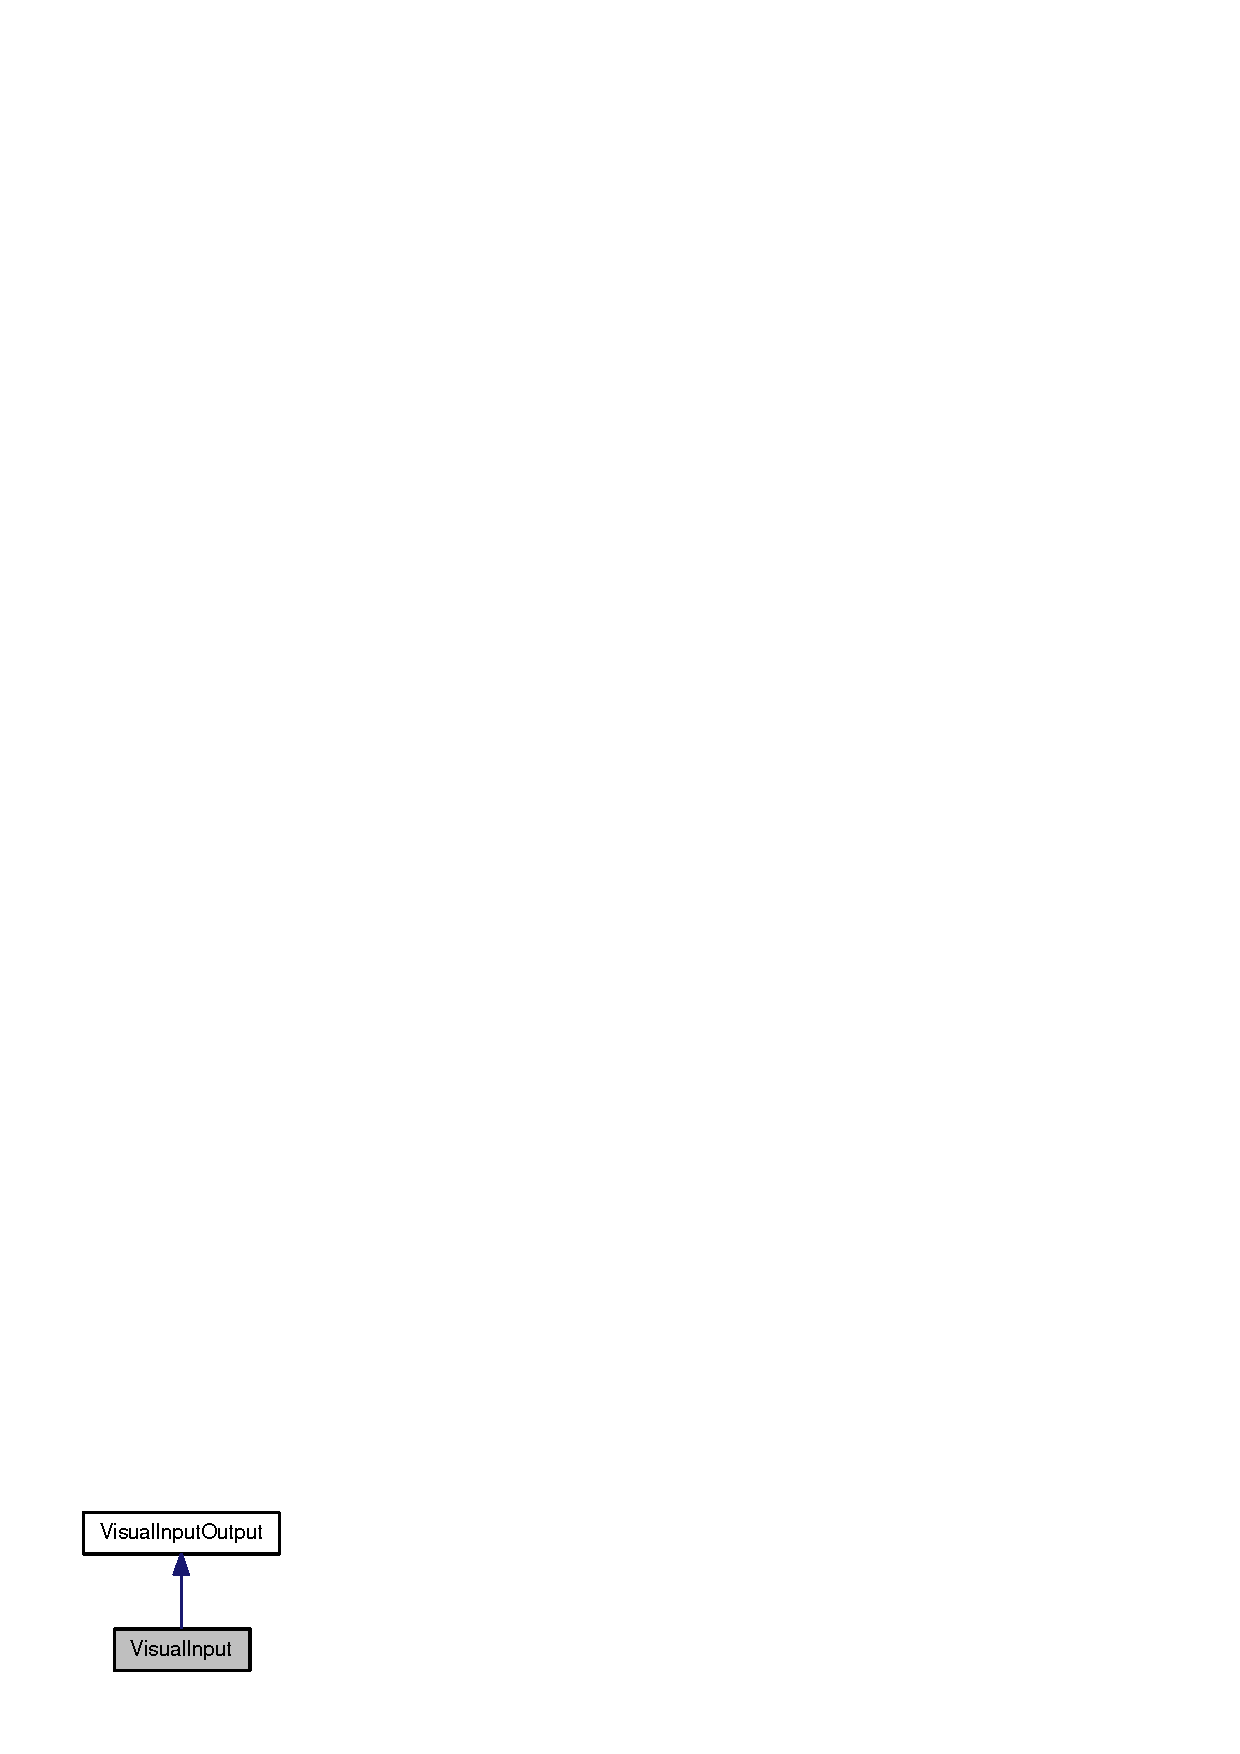
\includegraphics[width=69pt]{classVisualInput__inherit__graph}
\end{center}
\end{figure}
Collaboration diagram for VisualInput:\nopagebreak
\begin{figure}[H]
\begin{center}
\leavevmode
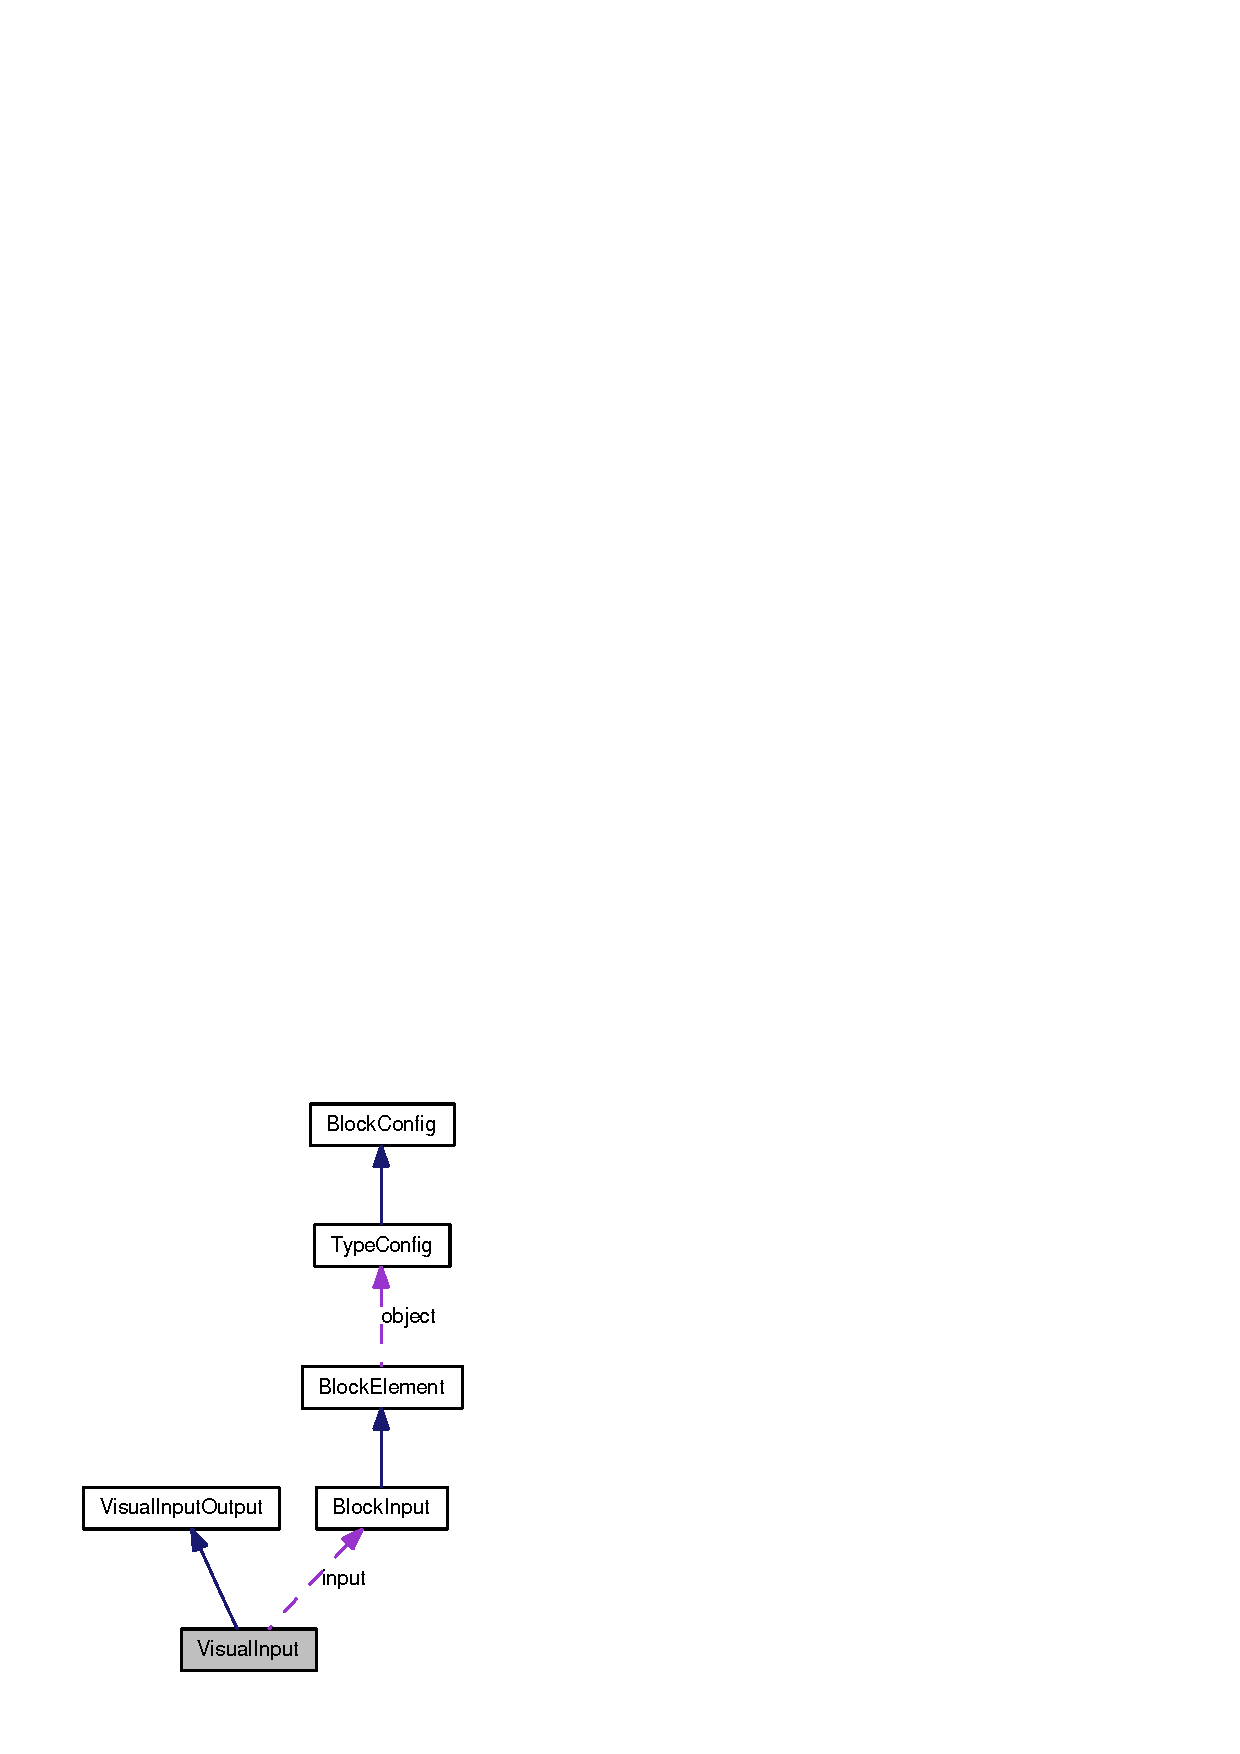
\includegraphics[width=112pt]{classVisualInput__coll__graph}
\end{center}
\end{figure}
\subsection*{Public Member Functions}
\begin{CompactItemize}
\item 
\_\-\_\-fastcall \hyperlink{classVisualInput_a4321580033604ae3c7b951b8061b8b5}{VisualInput} (Classes::TComponent $\ast$AOwner)
\end{CompactItemize}
\subsection*{Public Attributes}
\begin{CompactItemize}
\item 
\hyperlink{classBlockInput}{BlockInput} $\ast$ \hyperlink{classVisualInput_28567cf4de37faa89c1af357c19677e8}{input}
\end{CompactItemize}


\subsection{Detailed Description}
Klasa symbolizuje wizualne wejscie bloku 

Definition at line 13 of file VisualInput.h.

\subsection{Constructor \& Destructor Documentation}
\hypertarget{classVisualInput_a4321580033604ae3c7b951b8061b8b5}{
\index{VisualInput@{VisualInput}!VisualInput@{VisualInput}}
\index{VisualInput@{VisualInput}!VisualInput@{VisualInput}}
\subsubsection[VisualInput]{\setlength{\rightskip}{0pt plus 5cm}\_\-\_\-fastcall VisualInput::VisualInput (Classes::TComponent $\ast$ {\em AOwner})}}
\label{classVisualInput_a4321580033604ae3c7b951b8061b8b5}


Konstruktor \begin{Desc}
\item[Parameters:]
\begin{description}
\item[{\em AOwner}]wskaznik do klasy bedacej wlascicielem dla tej \end{description}
\end{Desc}


Definition at line 6 of file VisualInput.cpp.

References input.

\subsection{Member Data Documentation}
\hypertarget{classVisualInput_28567cf4de37faa89c1af357c19677e8}{
\index{VisualInput@{VisualInput}!input@{input}}
\index{input@{input}!VisualInput@{VisualInput}}
\subsubsection[input]{\setlength{\rightskip}{0pt plus 5cm}{\bf BlockInput}$\ast$ {\bf VisualInput::input}}}
\label{classVisualInput_28567cf4de37faa89c1af357c19677e8}


Wskaznik do wejscia bloku 

Definition at line 19 of file VisualInput.h.

Referenced by PIWOEngine::getConnectionTo(), PIWOEngine::MakeConnection(), PIWOEngine::OnVisualBlockInputHistoryClick(), VisualBlock::updateVisualComponents(), and VisualInput().

The documentation for this class was generated from the following files:\begin{CompactItemize}
\item 
/PIWO/Program/gui/\hyperlink{VisualInput_8h}{VisualInput.h}\item 
/PIWO/Program/gui/\hyperlink{VisualInput_8cpp}{VisualInput.cpp}\end{CompactItemize}

\hypertarget{classVisualInputOutput}{
\section{VisualInputOutput Class Reference}
\label{classVisualInputOutput}\index{VisualInputOutput@{VisualInputOutput}}
}
{\tt \#include $<$VisualInputOutput.h$>$}

Inheritance diagram for VisualInputOutput:\nopagebreak
\begin{figure}[H]
\begin{center}
\leavevmode
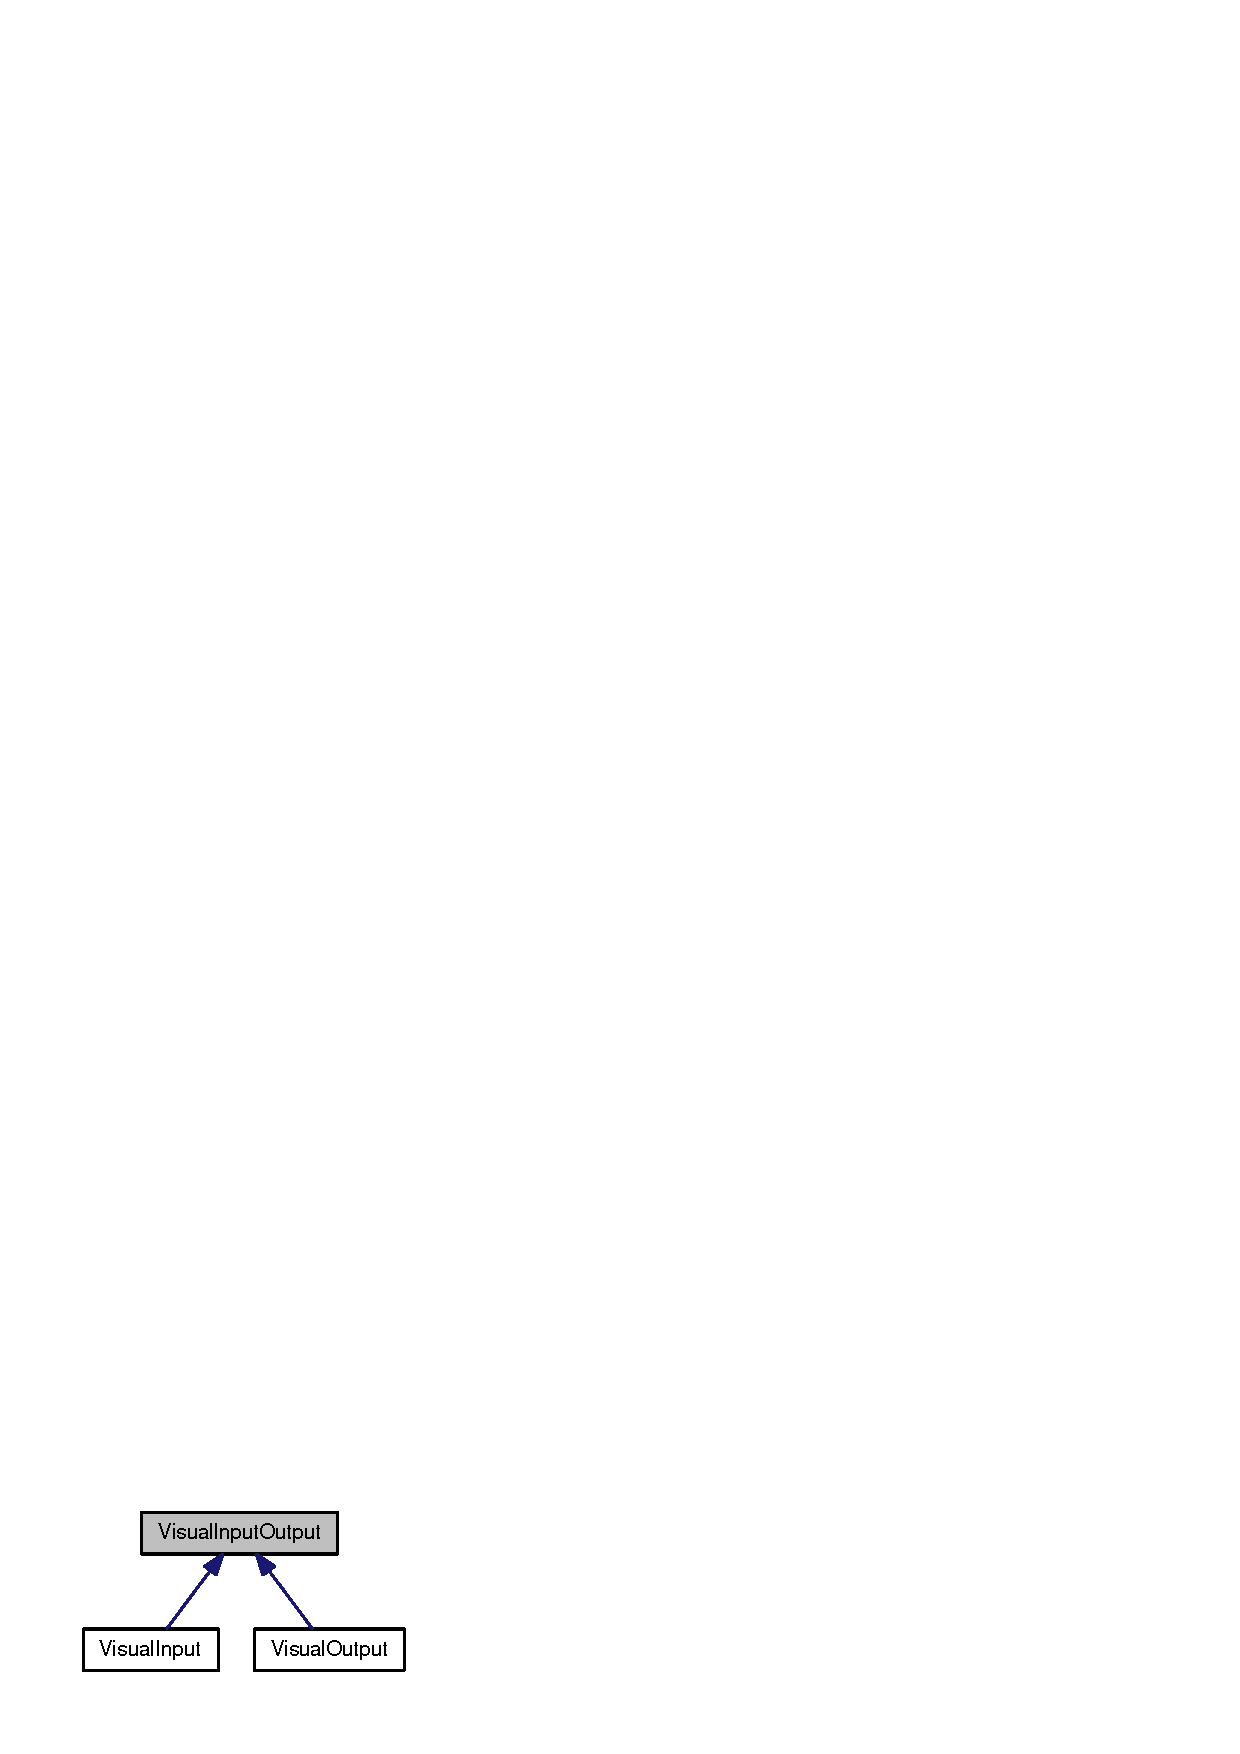
\includegraphics[width=99pt]{classVisualInputOutput__inherit__graph}
\end{center}
\end{figure}
\subsection*{Public Member Functions}
\begin{CompactItemize}
\item 
\_\-\_\-fastcall \hyperlink{classVisualInputOutput_0bd9a6f7a998c00f8bd5caf6e741cc80}{VisualInputOutput} (Classes::TComponent $\ast$AOwner)
\end{CompactItemize}
\subsection*{Public Attributes}
\begin{CompactItemize}
\item 
VisualFunction \hyperlink{classVisualInputOutput_b2f2b186575d7e87de055b36ce867c77}{OnShowHistory}
\end{CompactItemize}
\subsection*{Private Member Functions}
\begin{CompactItemize}
\item 
void \_\-\_\-fastcall \hyperlink{classVisualInputOutput_8821c8e38a799b89c34ec72274803090}{MouseEnterF} (TObject $\ast$Sender)
\item 
void \_\-\_\-fastcall \hyperlink{classVisualInputOutput_d92af8dbf5d8a282a9c3459415f3363d}{MouseLeaveF} (TObject $\ast$Sender)
\item 
void \_\-\_\-fastcall \hyperlink{classVisualInputOutput_e6c46a78d42ac09e36cff16974323573}{MouseDownF} (TObject $\ast$Sender, TMouseButton Button, TShiftState Shift, int X, int Y)
\end{CompactItemize}


\subsection{Detailed Description}
Klasa symbolizujaca wizualnie wejscia i wyjscia do bloku 

Definition at line 14 of file VisualInputOutput.h.

\subsection{Constructor \& Destructor Documentation}
\hypertarget{classVisualInputOutput_0bd9a6f7a998c00f8bd5caf6e741cc80}{
\index{VisualInputOutput@{VisualInputOutput}!VisualInputOutput@{VisualInputOutput}}
\index{VisualInputOutput@{VisualInputOutput}!VisualInputOutput@{VisualInputOutput}}
\subsubsection[VisualInputOutput]{\setlength{\rightskip}{0pt plus 5cm}\_\-\_\-fastcall VisualInputOutput::VisualInputOutput (Classes::TComponent $\ast$ {\em AOwner})}}
\label{classVisualInputOutput_0bd9a6f7a998c00f8bd5caf6e741cc80}


Konstruktor \begin{Desc}
\item[Parameters:]
\begin{description}
\item[{\em AOwner}]wskaznik do klasy bedacej wlascicielem dla tej \end{description}
\end{Desc}


Definition at line 6 of file VisualInputOutput.cpp.

References MouseDownF(), MouseEnterF(), MouseLeaveF(), and OnShowHistory.

\subsection{Member Function Documentation}
\hypertarget{classVisualInputOutput_8821c8e38a799b89c34ec72274803090}{
\index{VisualInputOutput@{VisualInputOutput}!MouseEnterF@{MouseEnterF}}
\index{MouseEnterF@{MouseEnterF}!VisualInputOutput@{VisualInputOutput}}
\subsubsection[MouseEnterF]{\setlength{\rightskip}{0pt plus 5cm}void \_\-\_\-fastcall VisualInputOutput::MouseEnterF (TObject $\ast$ {\em Sender})\hspace{0.3cm}{\tt  \mbox{[}private\mbox{]}}}}
\label{classVisualInputOutput_8821c8e38a799b89c34ec72274803090}




Definition at line 25 of file VisualInputOutput.cpp.

Referenced by VisualInputOutput().\hypertarget{classVisualInputOutput_d92af8dbf5d8a282a9c3459415f3363d}{
\index{VisualInputOutput@{VisualInputOutput}!MouseLeaveF@{MouseLeaveF}}
\index{MouseLeaveF@{MouseLeaveF}!VisualInputOutput@{VisualInputOutput}}
\subsubsection[MouseLeaveF]{\setlength{\rightskip}{0pt plus 5cm}void \_\-\_\-fastcall VisualInputOutput::MouseLeaveF (TObject $\ast$ {\em Sender})\hspace{0.3cm}{\tt  \mbox{[}private\mbox{]}}}}
\label{classVisualInputOutput_d92af8dbf5d8a282a9c3459415f3363d}




Definition at line 30 of file VisualInputOutput.cpp.

Referenced by VisualInputOutput().\hypertarget{classVisualInputOutput_e6c46a78d42ac09e36cff16974323573}{
\index{VisualInputOutput@{VisualInputOutput}!MouseDownF@{MouseDownF}}
\index{MouseDownF@{MouseDownF}!VisualInputOutput@{VisualInputOutput}}
\subsubsection[MouseDownF]{\setlength{\rightskip}{0pt plus 5cm}void \_\-\_\-fastcall VisualInputOutput::MouseDownF (TObject $\ast$ {\em Sender}, \/  TMouseButton {\em Button}, \/  TShiftState {\em Shift}, \/  int {\em X}, \/  int {\em Y})\hspace{0.3cm}{\tt  \mbox{[}private\mbox{]}}}}
\label{classVisualInputOutput_e6c46a78d42ac09e36cff16974323573}




Definition at line 35 of file VisualInputOutput.cpp.

References OnShowHistory.

Referenced by VisualInputOutput().

\subsection{Member Data Documentation}
\hypertarget{classVisualInputOutput_b2f2b186575d7e87de055b36ce867c77}{
\index{VisualInputOutput@{VisualInputOutput}!OnShowHistory@{OnShowHistory}}
\index{OnShowHistory@{OnShowHistory}!VisualInputOutput@{VisualInputOutput}}
\subsubsection[OnShowHistory]{\setlength{\rightskip}{0pt plus 5cm}VisualFunction {\bf VisualInputOutput::OnShowHistory}}}
\label{classVisualInputOutput_b2f2b186575d7e87de055b36ce867c77}


Event 

Definition at line 25 of file VisualInputOutput.h.

Referenced by MouseDownF(), VisualBlock::updateVisualComponents(), and VisualInputOutput().

The documentation for this class was generated from the following files:\begin{CompactItemize}
\item 
/PIWO/Program/gui/\hyperlink{VisualInputOutput_8h}{VisualInputOutput.h}\item 
/PIWO/Program/gui/\hyperlink{VisualInputOutput_8cpp}{VisualInputOutput.cpp}\end{CompactItemize}

\hypertarget{classVisualOutput}{
\section{VisualOutput Class Reference}
\label{classVisualOutput}\index{VisualOutput@{VisualOutput}}
}
{\tt \#include $<$VisualOutput.h$>$}

Inheritance diagram for VisualOutput:\nopagebreak
\begin{figure}[H]
\begin{center}
\leavevmode
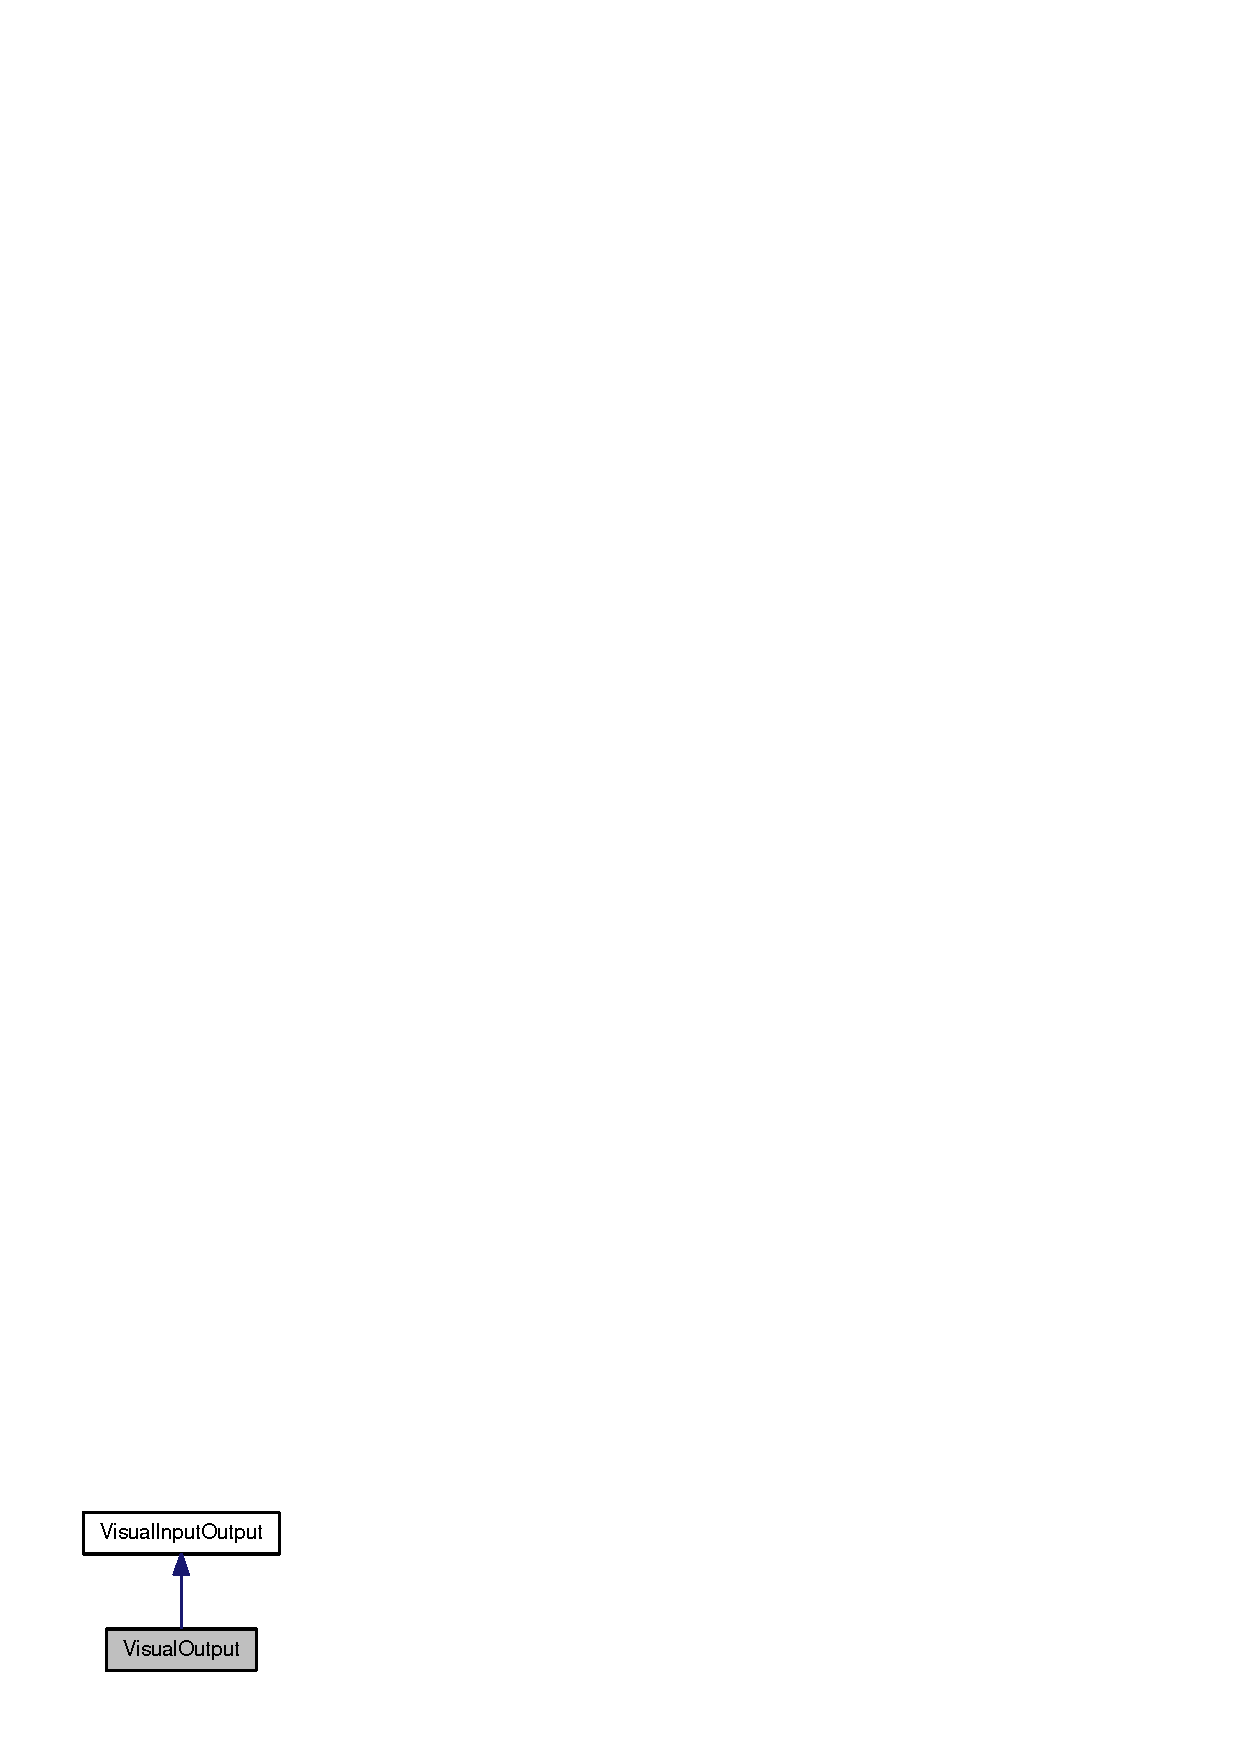
\includegraphics[width=69pt]{classVisualOutput__inherit__graph}
\end{center}
\end{figure}
Collaboration diagram for VisualOutput:\nopagebreak
\begin{figure}[H]
\begin{center}
\leavevmode
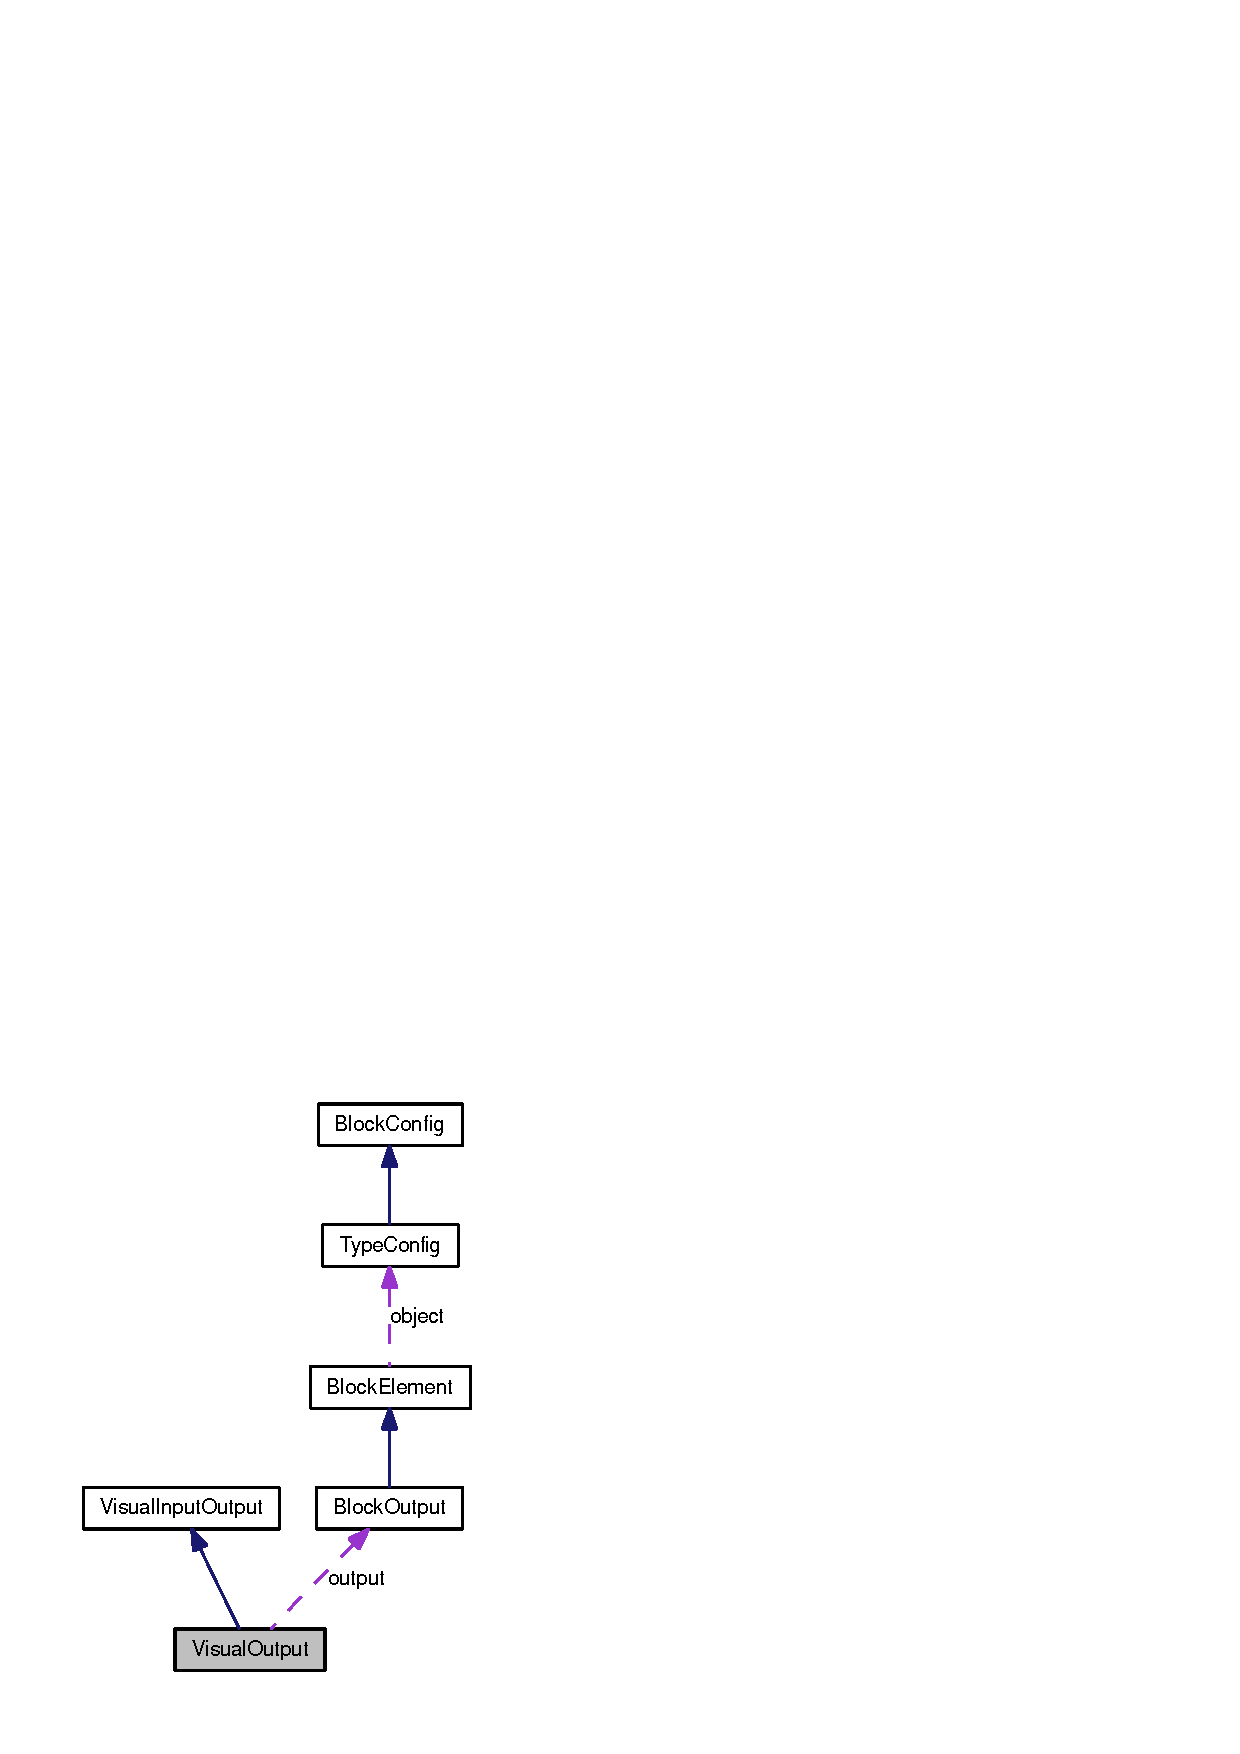
\includegraphics[width=114pt]{classVisualOutput__coll__graph}
\end{center}
\end{figure}
\subsection*{Public Member Functions}
\begin{CompactItemize}
\item 
\_\-\_\-fastcall \hyperlink{classVisualOutput_f194cf1b45bd799a81ffa0220653a161}{VisualOutput} (Classes::TComponent $\ast$AOwner)
\end{CompactItemize}
\subsection*{Public Attributes}
\begin{CompactItemize}
\item 
\hyperlink{classBlockOutput}{BlockOutput} $\ast$ \hyperlink{classVisualOutput_1514ca043572331039b22002581a22f8}{output}
\end{CompactItemize}


\subsection{Detailed Description}
Klasa symbolizujaca wizualne wyjscia z bloku 

Definition at line 14 of file VisualOutput.h.

\subsection{Constructor \& Destructor Documentation}
\hypertarget{classVisualOutput_f194cf1b45bd799a81ffa0220653a161}{
\index{VisualOutput@{VisualOutput}!VisualOutput@{VisualOutput}}
\index{VisualOutput@{VisualOutput}!VisualOutput@{VisualOutput}}
\subsubsection[VisualOutput]{\setlength{\rightskip}{0pt plus 5cm}\_\-\_\-fastcall VisualOutput::VisualOutput (Classes::TComponent $\ast$ {\em AOwner})}}
\label{classVisualOutput_f194cf1b45bd799a81ffa0220653a161}


Konstruktor \begin{Desc}
\item[Parameters:]
\begin{description}
\item[{\em AOwner}]wskaznik do klasy bedacej wlascicielem dla tej \end{description}
\end{Desc}


Definition at line 6 of file VisualOutput.cpp.

References output.

\subsection{Member Data Documentation}
\hypertarget{classVisualOutput_1514ca043572331039b22002581a22f8}{
\index{VisualOutput@{VisualOutput}!output@{output}}
\index{output@{output}!VisualOutput@{VisualOutput}}
\subsubsection[output]{\setlength{\rightskip}{0pt plus 5cm}{\bf BlockOutput}$\ast$ {\bf VisualOutput::output}}}
\label{classVisualOutput_1514ca043572331039b22002581a22f8}


Wskaznik do wyjscia 

Definition at line 20 of file VisualOutput.h.

Referenced by PIWOEngine::MakeConnection(), PIWOEngine::OnVisualBlockInputSelected(), PIWOEngine::OnVisualBlockOutputHistoryClick(), PIWOEngine::OnVisualBlockOutputSelected(), VisualBlock::updateVisualComponents(), and VisualOutput().

The documentation for this class was generated from the following files:\begin{CompactItemize}
\item 
/PIWO/Program/gui/\hyperlink{VisualOutput_8h}{VisualOutput.h}\item 
/PIWO/Program/gui/\hyperlink{VisualOutput_8cpp}{VisualOutput.cpp}\end{CompactItemize}

\chapter{File Documentation}
\hypertarget{FunctionDLL_8cpp}{
\section{/PIWO/Program/brige/FunctionDLL.cpp File Reference}
\label{FunctionDLL_8cpp}\index{/PIWO/Program/brige/FunctionDLL.cpp@{/PIWO/Program/brige/FunctionDLL.cpp}}
}
{\tt \#include \char`\"{}FunctionDLL.h\char`\"{}}\par


Include dependency graph for FunctionDLL.cpp:\nopagebreak
\begin{figure}[H]
\begin{center}
\leavevmode
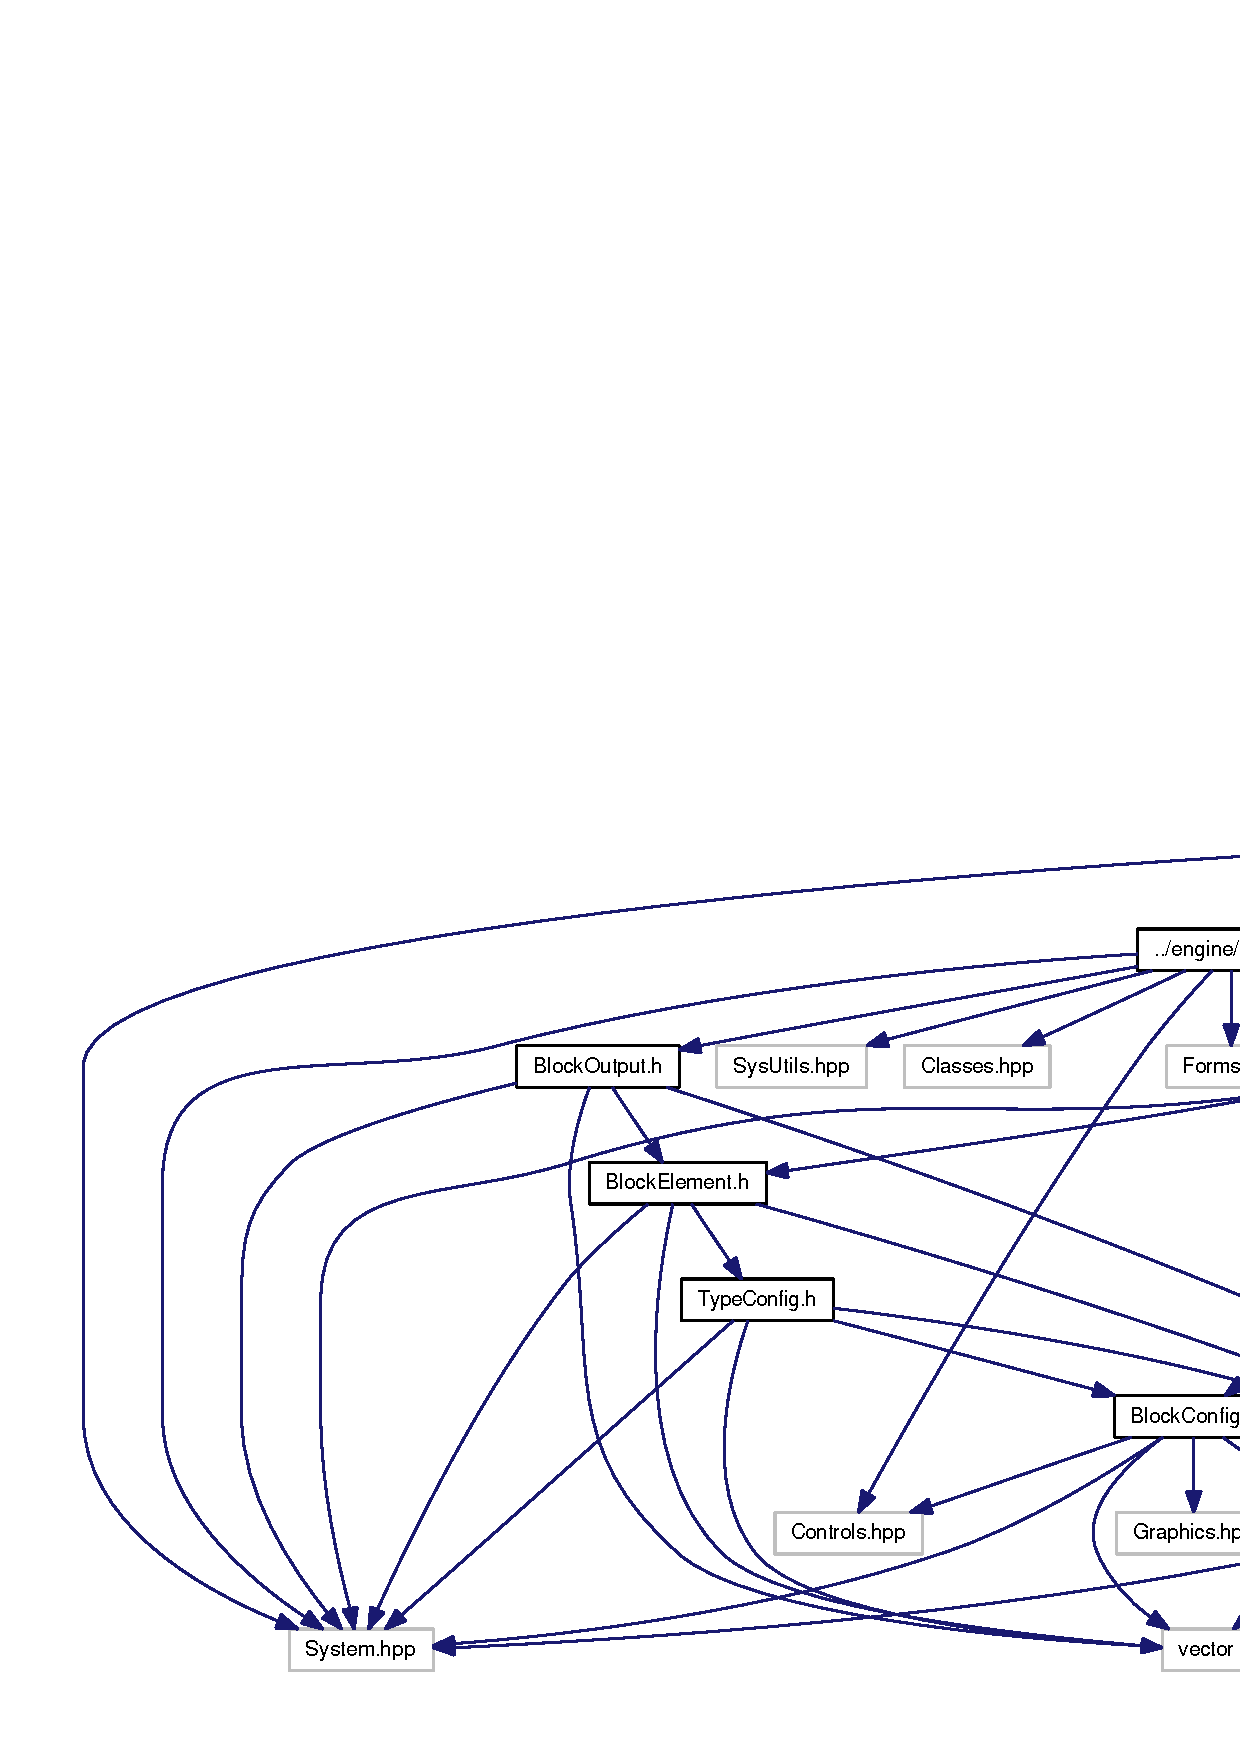
\includegraphics[width=420pt]{FunctionDLL_8cpp__incl}
\end{center}
\end{figure}

\hypertarget{FunctionDLL_8h}{
\section{/PIWO/Program/brige/FunctionDLL.h File Reference}
\label{FunctionDLL_8h}\index{/PIWO/Program/brige/FunctionDLL.h@{/PIWO/Program/brige/FunctionDLL.h}}
}
{\tt \#include $<$System.hpp$>$}\par
{\tt \#include $<$vector$>$}\par
{\tt \#include $<$exception$>$}\par
{\tt \#include $<$IniFiles.hpp$>$}\par
{\tt \#include \char`\"{}../engine/Block.h\char`\"{}}\par


Include dependency graph for FunctionDLL.h:\nopagebreak
\begin{figure}[H]
\begin{center}
\leavevmode
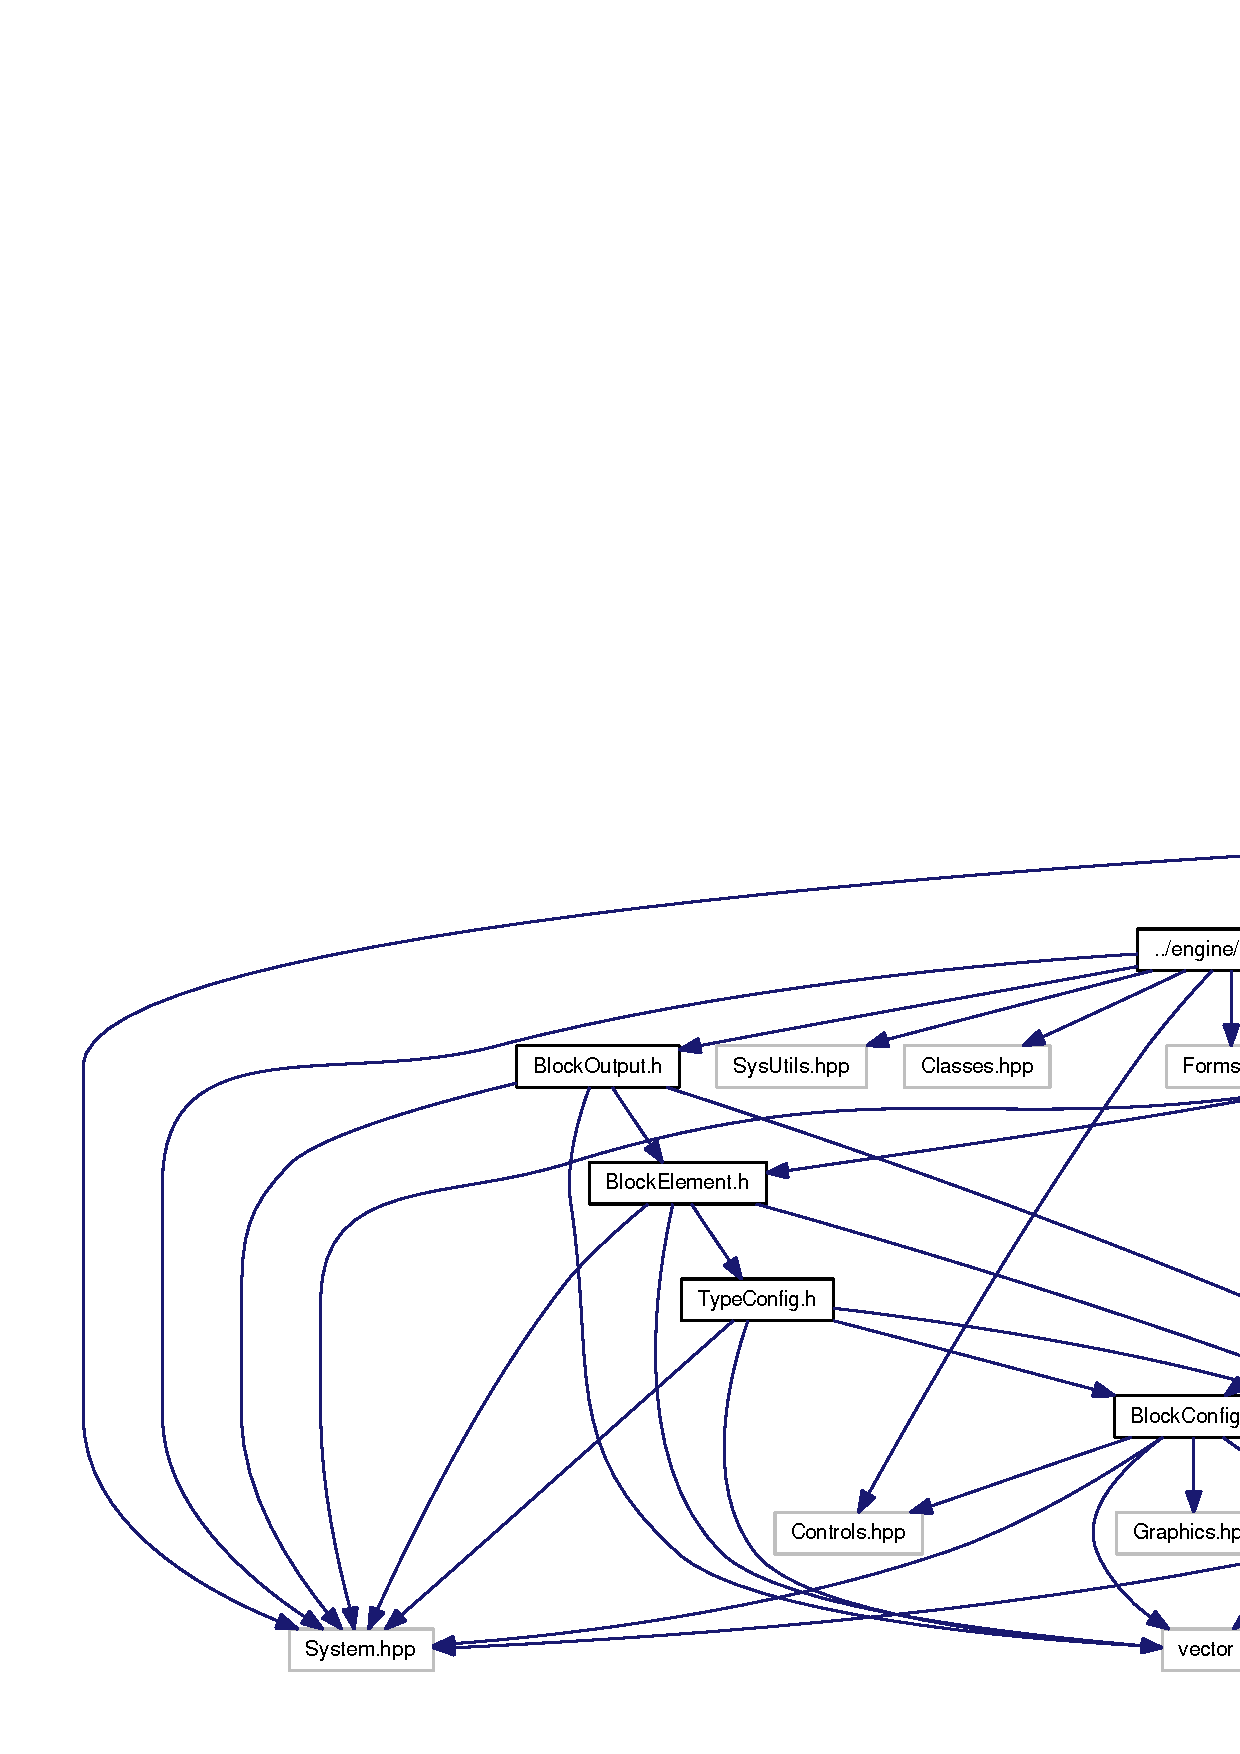
\includegraphics[width=420pt]{FunctionDLL_8h__incl}
\end{center}
\end{figure}


This graph shows which files directly or indirectly include this file:\nopagebreak
\begin{figure}[H]
\begin{center}
\leavevmode
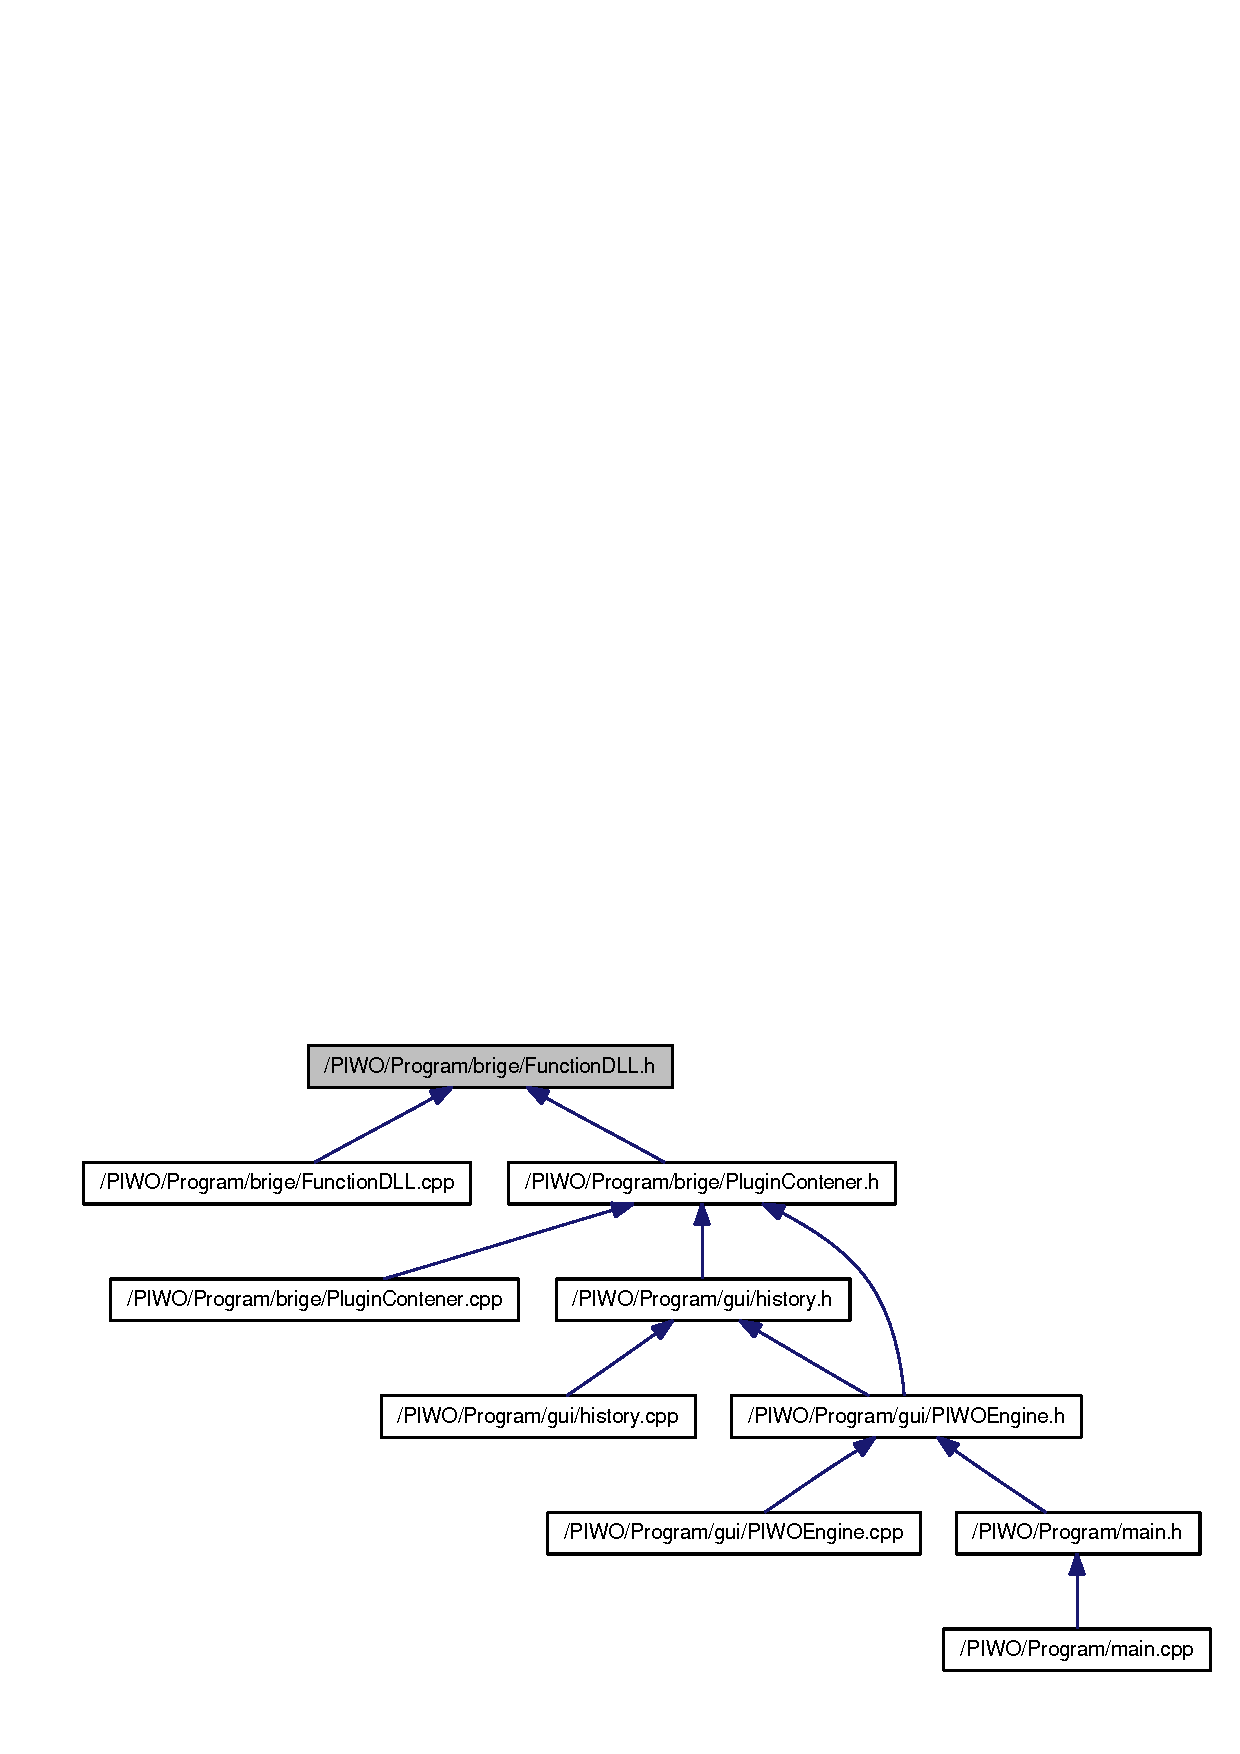
\includegraphics[width=292pt]{FunctionDLL_8h__dep__incl}
\end{center}
\end{figure}
\subsection*{Classes}
\begin{CompactItemize}
\item 
class \hyperlink{classFunctionDLL}{FunctionDLL}
\end{CompactItemize}
\subsection*{Typedefs}
\begin{CompactItemize}
\item 
typedef \hyperlink{classBlock}{Block} $\ast$typedef \hyperlink{FunctionDLL_8h_c612ada38bf83be79acb2154e3f72be6}{int} (\_\-\_\-stdcall $\ast$FunctionDLL\_\-validate)(\hyperlink{classBlock}{Block} $\ast$)
\end{CompactItemize}
\subsection*{Functions}
\begin{CompactItemize}
\item 
typedef \hyperlink{FunctionDLL_8h_2854864c4eeedd04786b0fafe1da1165}{int} (\_\-\_\-stdcall $\ast$FunctionDLL\_\-run)(\hyperlink{classBlock}{Block} $\ast$)
\item 
typedef \hyperlink{FunctionDLL_8h_9c362bc12556d578110b09d4563a7ed4}{bool} (\_\-\_\-stdcall $\ast$FunctionDLL\_\-showConfig)(TComponent $\ast$
\item 
typedef \hyperlink{FunctionDLL_8h_10f738c80bfc69a75e5d249561e4a81b}{void} (\_\-\_\-closure $\ast$FunctionDLL\_\-onClick)(void $\ast$)
\end{CompactItemize}


\subsection{Typedef Documentation}
\hypertarget{FunctionDLL_8h_c612ada38bf83be79acb2154e3f72be6}{
\index{FunctionDLL.h@{FunctionDLL.h}!int@{int}}
\index{int@{int}!FunctionDLL.h@{FunctionDLL.h}}
\subsubsection[int]{\setlength{\rightskip}{0pt plus 5cm}typedef TObject $\ast$typedef TObject $\ast$typedef TObject $\ast$typedef TObject $\ast$typedef int (\_\-\_\-stdcall $\ast$ {\em FunctionDLL\_\-validate})}}
\label{FunctionDLL_8h_c612ada38bf83be79acb2154e3f72be6}




Definition at line 14 of file FunctionDLL.h.

\subsection{Function Documentation}
\hypertarget{FunctionDLL_8h_9c362bc12556d578110b09d4563a7ed4}{
\index{FunctionDLL.h@{FunctionDLL.h}!bool@{bool}}
\index{bool@{bool}!FunctionDLL.h@{FunctionDLL.h}}
\subsubsection[bool]{\setlength{\rightskip}{0pt plus 5cm}typedef bool (\_\-\_\-stdcall $\ast$ {\em FunctionDLL\_\-showConfig})}}
\label{FunctionDLL_8h_9c362bc12556d578110b09d4563a7ed4}


\hypertarget{FunctionDLL_8h_2854864c4eeedd04786b0fafe1da1165}{
\index{FunctionDLL.h@{FunctionDLL.h}!int@{int}}
\index{int@{int}!FunctionDLL.h@{FunctionDLL.h}}
\subsubsection[int]{\setlength{\rightskip}{0pt plus 5cm}typedef int (\_\-\_\-stdcall $\ast$ {\em FunctionDLL\_\-run})}}
\label{FunctionDLL_8h_2854864c4eeedd04786b0fafe1da1165}


\hypertarget{FunctionDLL_8h_10f738c80bfc69a75e5d249561e4a81b}{
\index{FunctionDLL.h@{FunctionDLL.h}!void@{void}}
\index{void@{void}!FunctionDLL.h@{FunctionDLL.h}}
\subsubsection[void]{\setlength{\rightskip}{0pt plus 5cm}typedef TObject $\ast$typedef TObject $\ast$typedef TObject $\ast$typedef TObject $\ast$typedef void(\_\-\_\-closure $\ast$VisualBlock\_\-FunctionMove)(TObject $\ast$ (\_\-\_\-closure $\ast$ {\em FunctionDLL\_\-onClick})}}
\label{FunctionDLL_8h_10f738c80bfc69a75e5d249561e4a81b}



\hypertarget{PluginContener_8cpp}{
\section{/PIWO/Program/brige/PluginContener.cpp File Reference}
\label{PluginContener_8cpp}\index{/PIWO/Program/brige/PluginContener.cpp@{/PIWO/Program/brige/PluginContener.cpp}}
}
{\tt \#include \char`\"{}PluginContener.h\char`\"{}}\par


Include dependency graph for PluginContener.cpp:\nopagebreak
\begin{figure}[H]
\begin{center}
\leavevmode
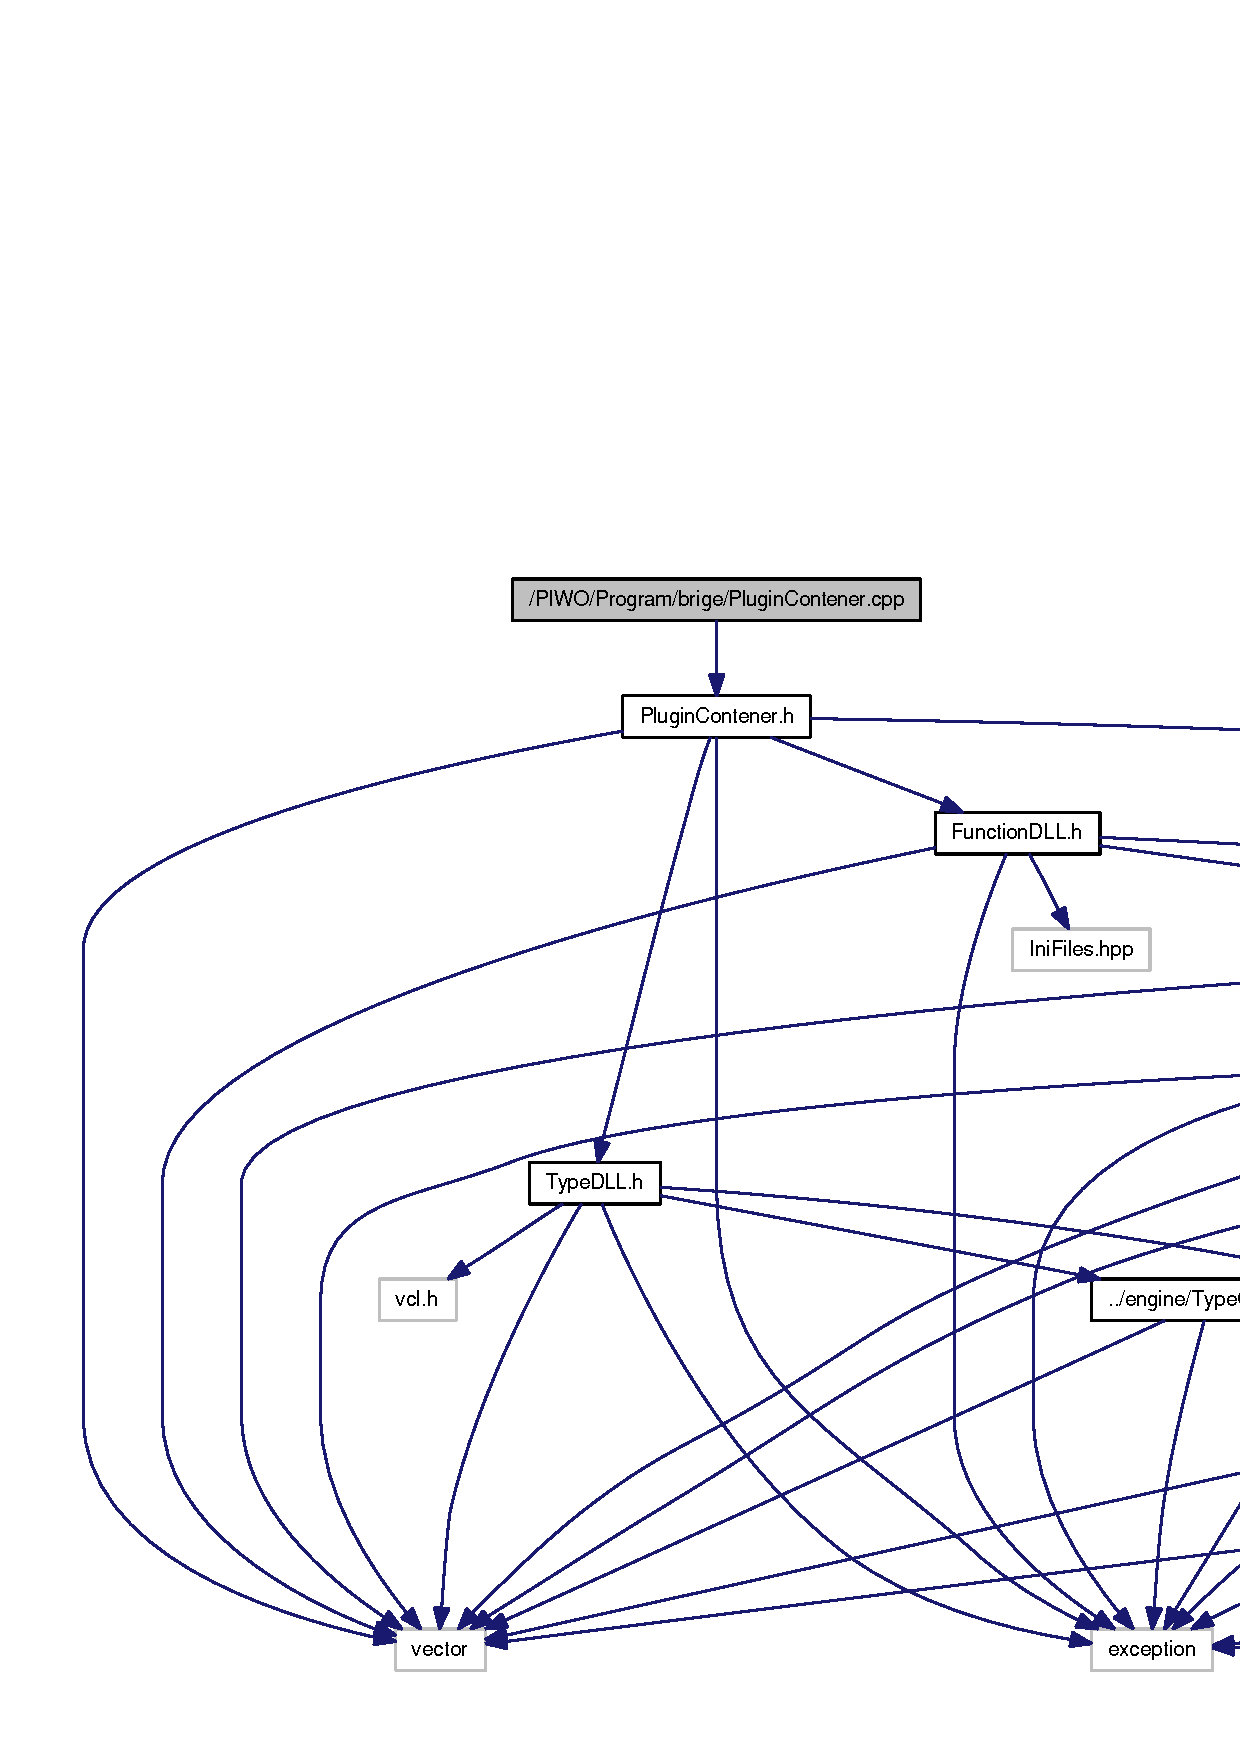
\includegraphics[width=420pt]{PluginContener_8cpp__incl}
\end{center}
\end{figure}

\hypertarget{PluginContener_8h}{
\section{/PIWO/Program/brige/PluginContener.h File Reference}
\label{PluginContener_8h}\index{/PIWO/Program/brige/PluginContener.h@{/PIWO/Program/brige/PluginContener.h}}
}
{\tt \#include $<$System.hpp$>$}\par
{\tt \#include $<$vector$>$}\par
{\tt \#include $<$exception$>$}\par
{\tt \#include \char`\"{}TypeDLL.h\char`\"{}}\par
{\tt \#include \char`\"{}FunctionDLL.h\char`\"{}}\par


Include dependency graph for PluginContener.h:\nopagebreak
\begin{figure}[H]
\begin{center}
\leavevmode
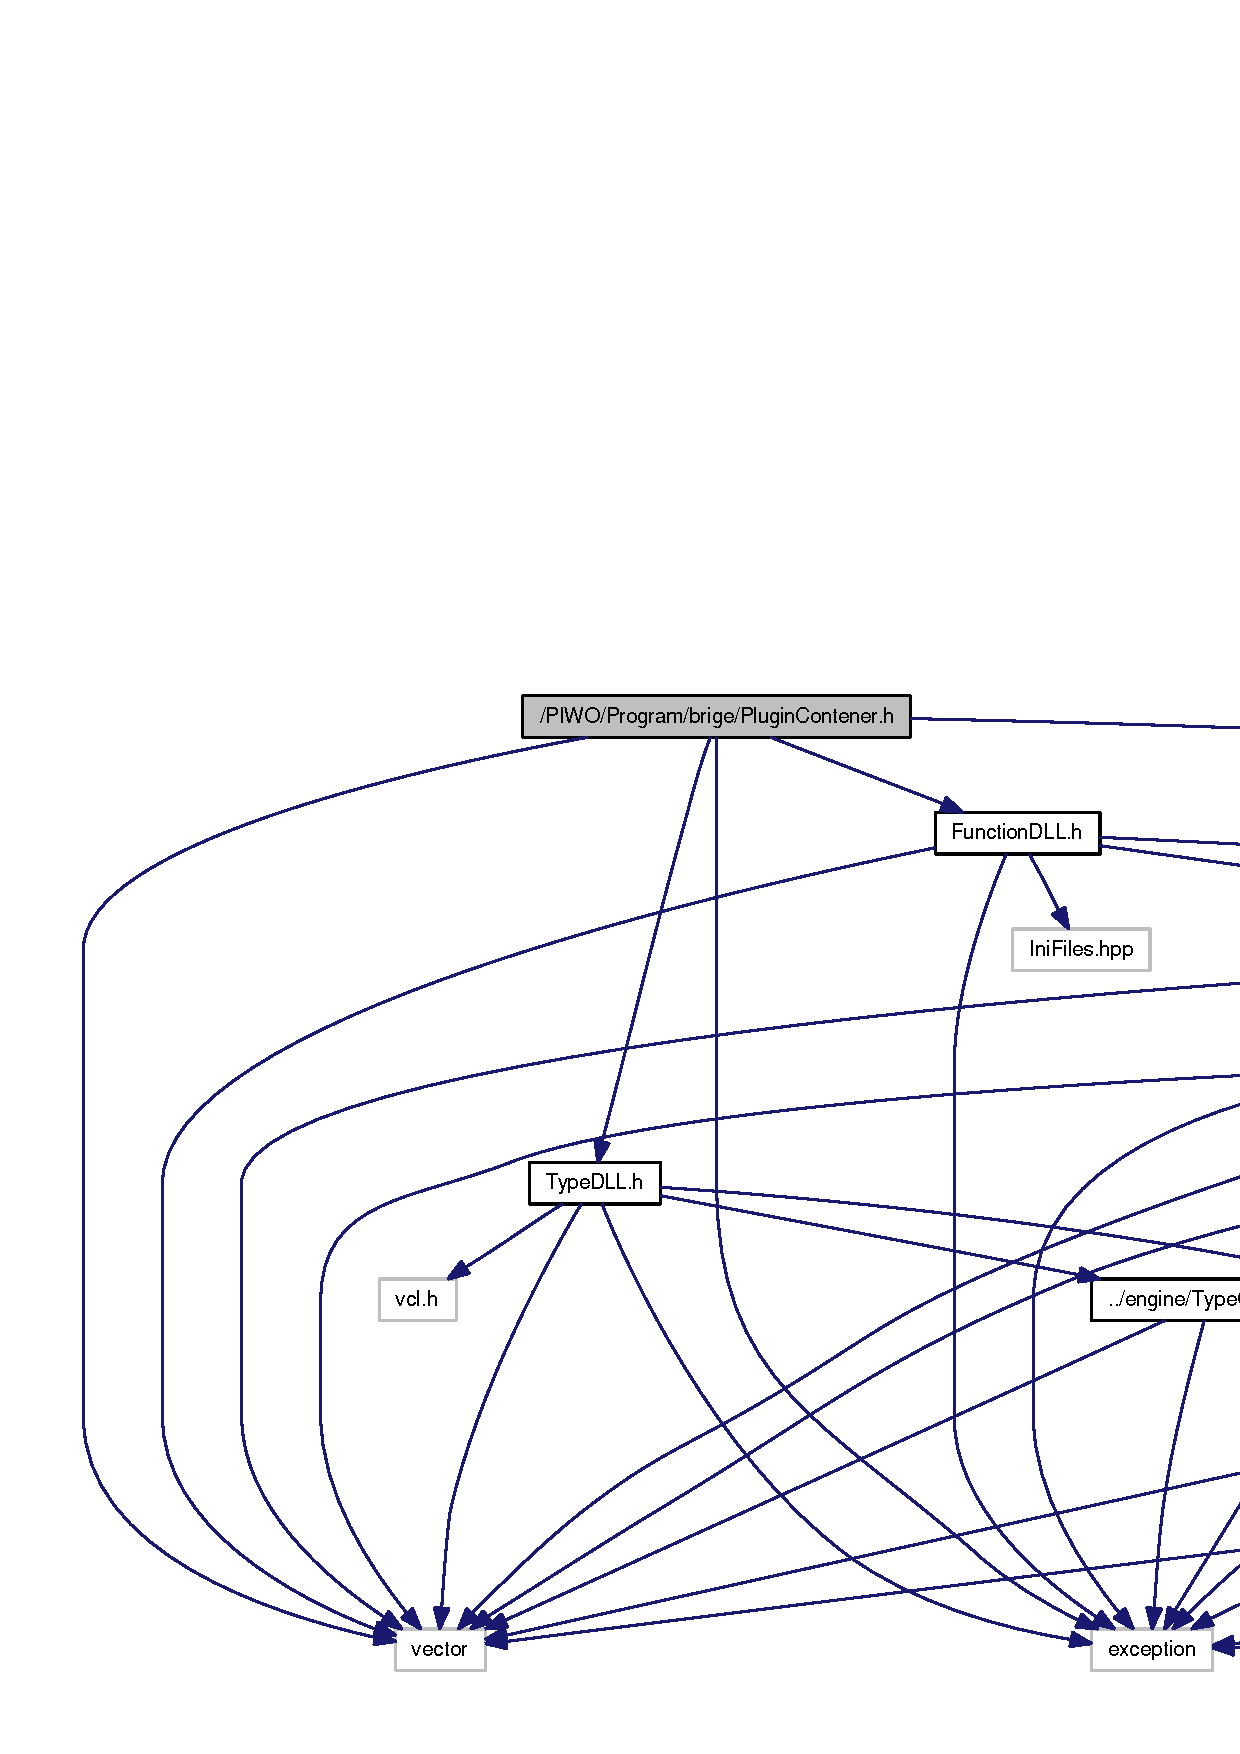
\includegraphics[width=420pt]{PluginContener_8h__incl}
\end{center}
\end{figure}


This graph shows which files directly or indirectly include this file:\nopagebreak
\begin{figure}[H]
\begin{center}
\leavevmode
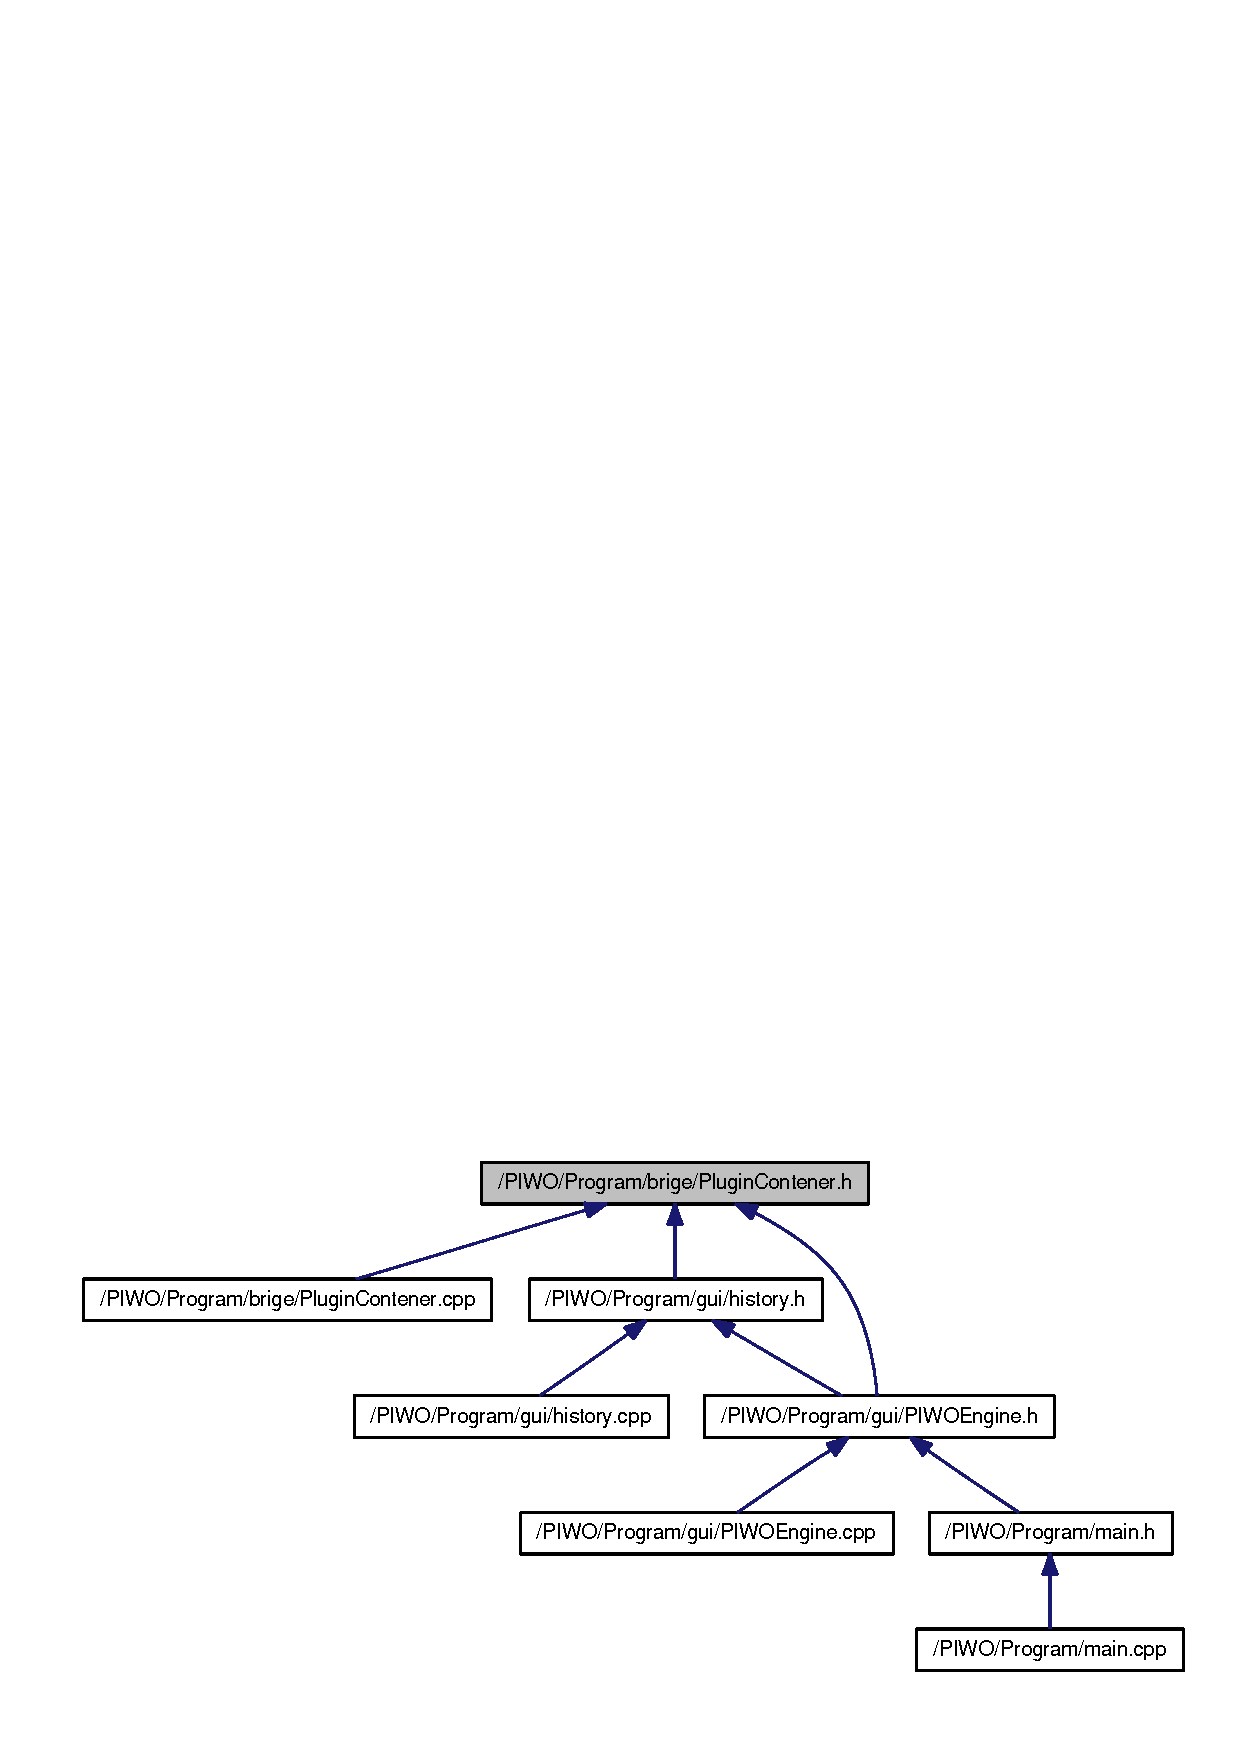
\includegraphics[width=286pt]{PluginContener_8h__dep__incl}
\end{center}
\end{figure}
\subsection*{Classes}
\begin{CompactItemize}
\item 
class \hyperlink{classPluginContener}{PluginContener}
\end{CompactItemize}
\subsection*{Typedefs}
\begin{CompactItemize}
\item 
typedef void(\_\-\_\-closure $\ast$ \hyperlink{PluginContener_8h_6050db466be0b09e7cdf5c163966f217}{PluginContener\_\-OnProgress} )(void $\ast$, int, int, AnsiString, int)
\item 
typedef const \hyperlink{PluginContener_8h_ae0fdfb65731fcd8dad6e5c841767865}{AnsiString}
\end{CompactItemize}
\subsection*{Functions}
\begin{CompactItemize}
\item 
typedef \hyperlink{PluginContener_8h_4e01b3c7ce148523393450a4775b8a4b}{void} (\_\-\_\-closure $\ast$PluginContener\_\-Log)(TObject $\ast$
\end{CompactItemize}


\subsection{Typedef Documentation}
\hypertarget{PluginContener_8h_ae0fdfb65731fcd8dad6e5c841767865}{
\index{PluginContener.h@{PluginContener.h}!AnsiString@{AnsiString}}
\index{AnsiString@{AnsiString}!PluginContener.h@{PluginContener.h}}
\subsubsection[AnsiString]{\setlength{\rightskip}{0pt plus 5cm}typedef const AnsiString}}
\label{PluginContener_8h_ae0fdfb65731fcd8dad6e5c841767865}




Definition at line 10 of file PluginContener.h.\hypertarget{PluginContener_8h_6050db466be0b09e7cdf5c163966f217}{
\index{PluginContener.h@{PluginContener.h}!PluginContener\_\-OnProgress@{PluginContener\_\-OnProgress}}
\index{PluginContener\_\-OnProgress@{PluginContener\_\-OnProgress}!PluginContener.h@{PluginContener.h}}
\subsubsection[PluginContener\_\-OnProgress]{\setlength{\rightskip}{0pt plus 5cm}typedef void(\_\-\_\-closure $\ast$ {\bf PluginContener\_\-OnProgress})(void $\ast$, int, int, AnsiString, int)}}
\label{PluginContener_8h_6050db466be0b09e7cdf5c163966f217}




Definition at line 9 of file PluginContener.h.

\subsection{Function Documentation}
\hypertarget{PluginContener_8h_4e01b3c7ce148523393450a4775b8a4b}{
\index{PluginContener.h@{PluginContener.h}!void@{void}}
\index{void@{void}!PluginContener.h@{PluginContener.h}}
\subsubsection[void]{\setlength{\rightskip}{0pt plus 5cm}typedef void (\_\-\_\-closure $\ast$ {\em PluginContener\_\-Log})}}
\label{PluginContener_8h_4e01b3c7ce148523393450a4775b8a4b}



\hypertarget{TypeDLL_8cpp}{
\section{/PIWO/Program/brige/TypeDLL.cpp File Reference}
\label{TypeDLL_8cpp}\index{/PIWO/Program/brige/TypeDLL.cpp@{/PIWO/Program/brige/TypeDLL.cpp}}
}
{\tt \#include \char`\"{}TypeDLL.h\char`\"{}}\par


Include dependency graph for TypeDLL.cpp:\nopagebreak
\begin{figure}[H]
\begin{center}
\leavevmode
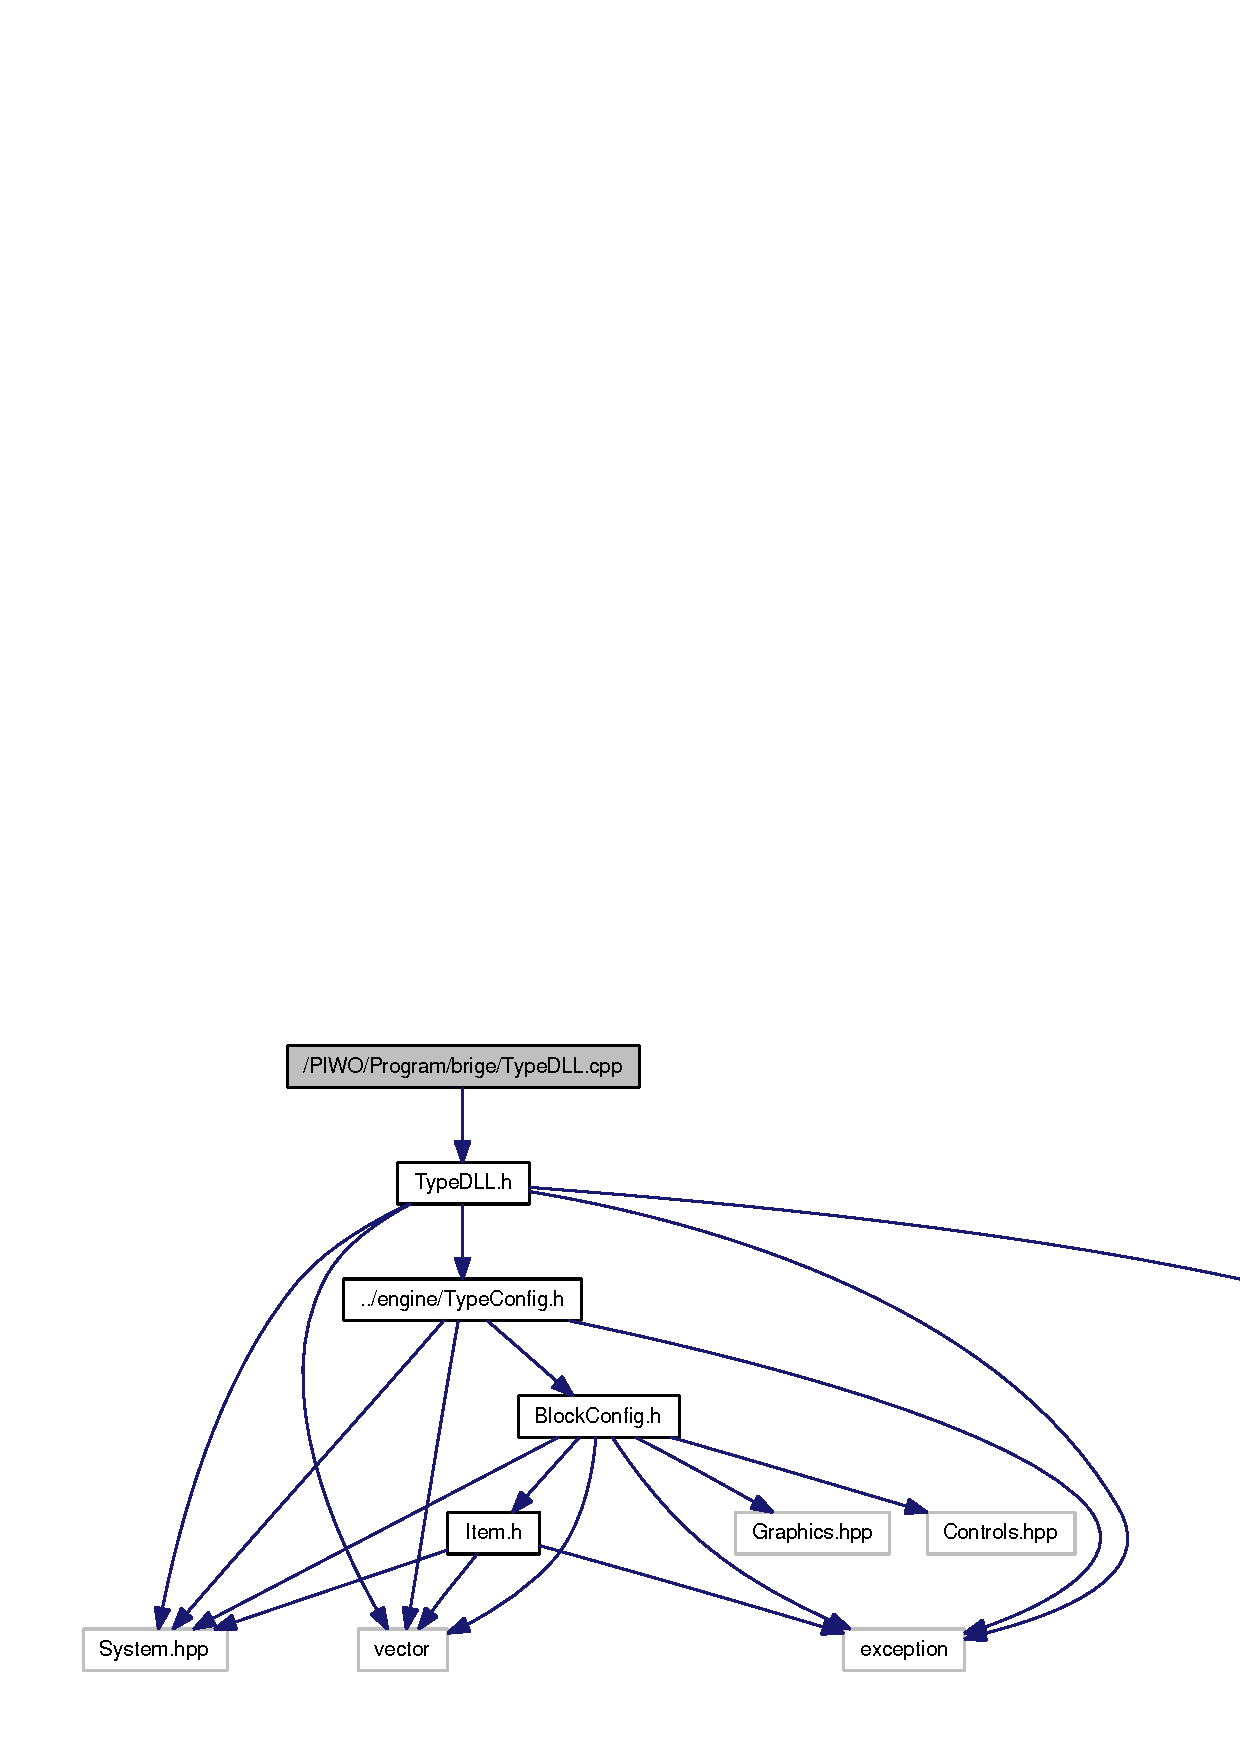
\includegraphics[width=324pt]{TypeDLL_8cpp__incl}
\end{center}
\end{figure}

\hypertarget{TypeDLL_8h}{
\section{/PIWO/Program/brige/TypeDLL.h File Reference}
\label{TypeDLL_8h}\index{/PIWO/Program/brige/TypeDLL.h@{/PIWO/Program/brige/TypeDLL.h}}
}
{\tt \#include $<$System.hpp$>$}\par
{\tt \#include $<$vector$>$}\par
{\tt \#include $<$exception$>$}\par
{\tt \#include $<$vcl.h$>$}\par
{\tt \#include \char`\"{}../engine/TypeConfig.h\char`\"{}}\par


Include dependency graph for TypeDLL.h:\nopagebreak
\begin{figure}[H]
\begin{center}
\leavevmode
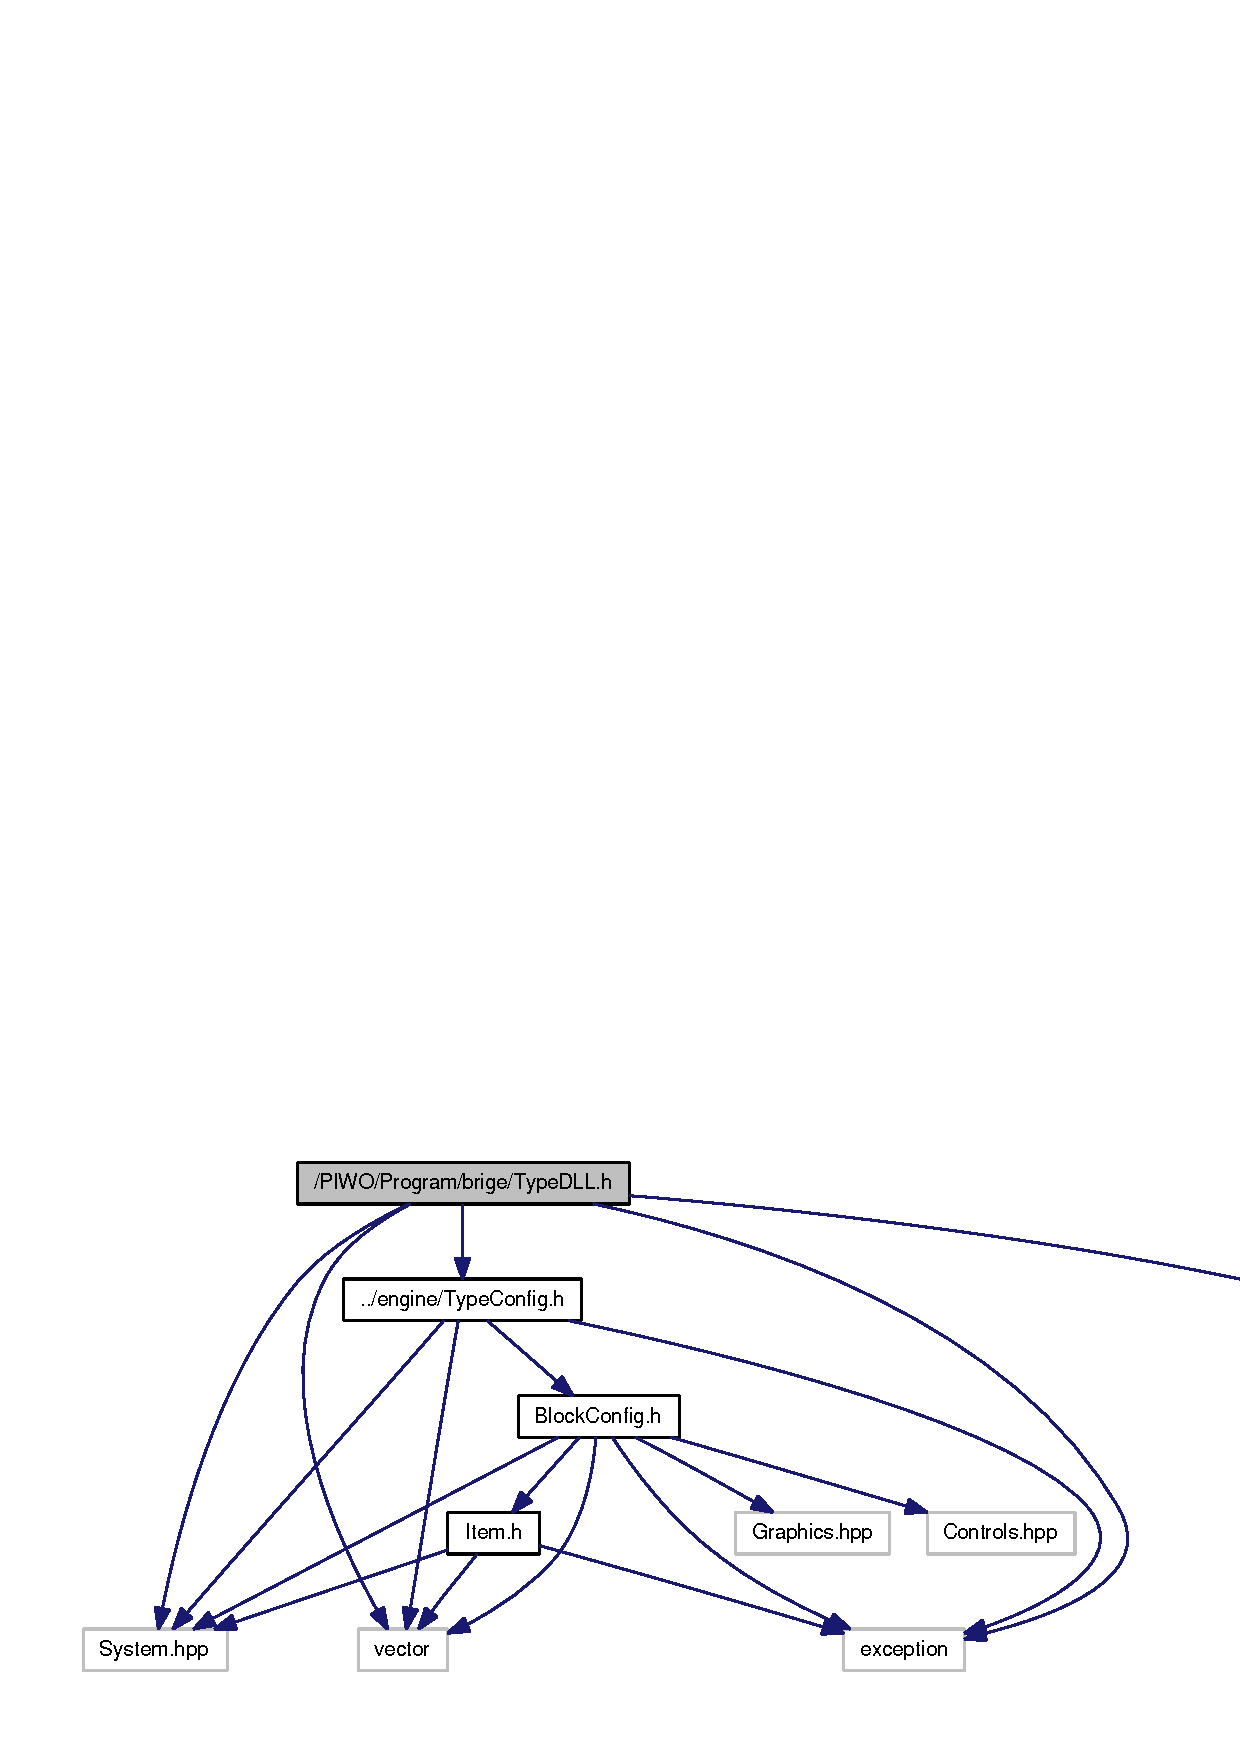
\includegraphics[width=324pt]{TypeDLL_8h__incl}
\end{center}
\end{figure}


This graph shows which files directly or indirectly include this file:\nopagebreak
\begin{figure}[H]
\begin{center}
\leavevmode
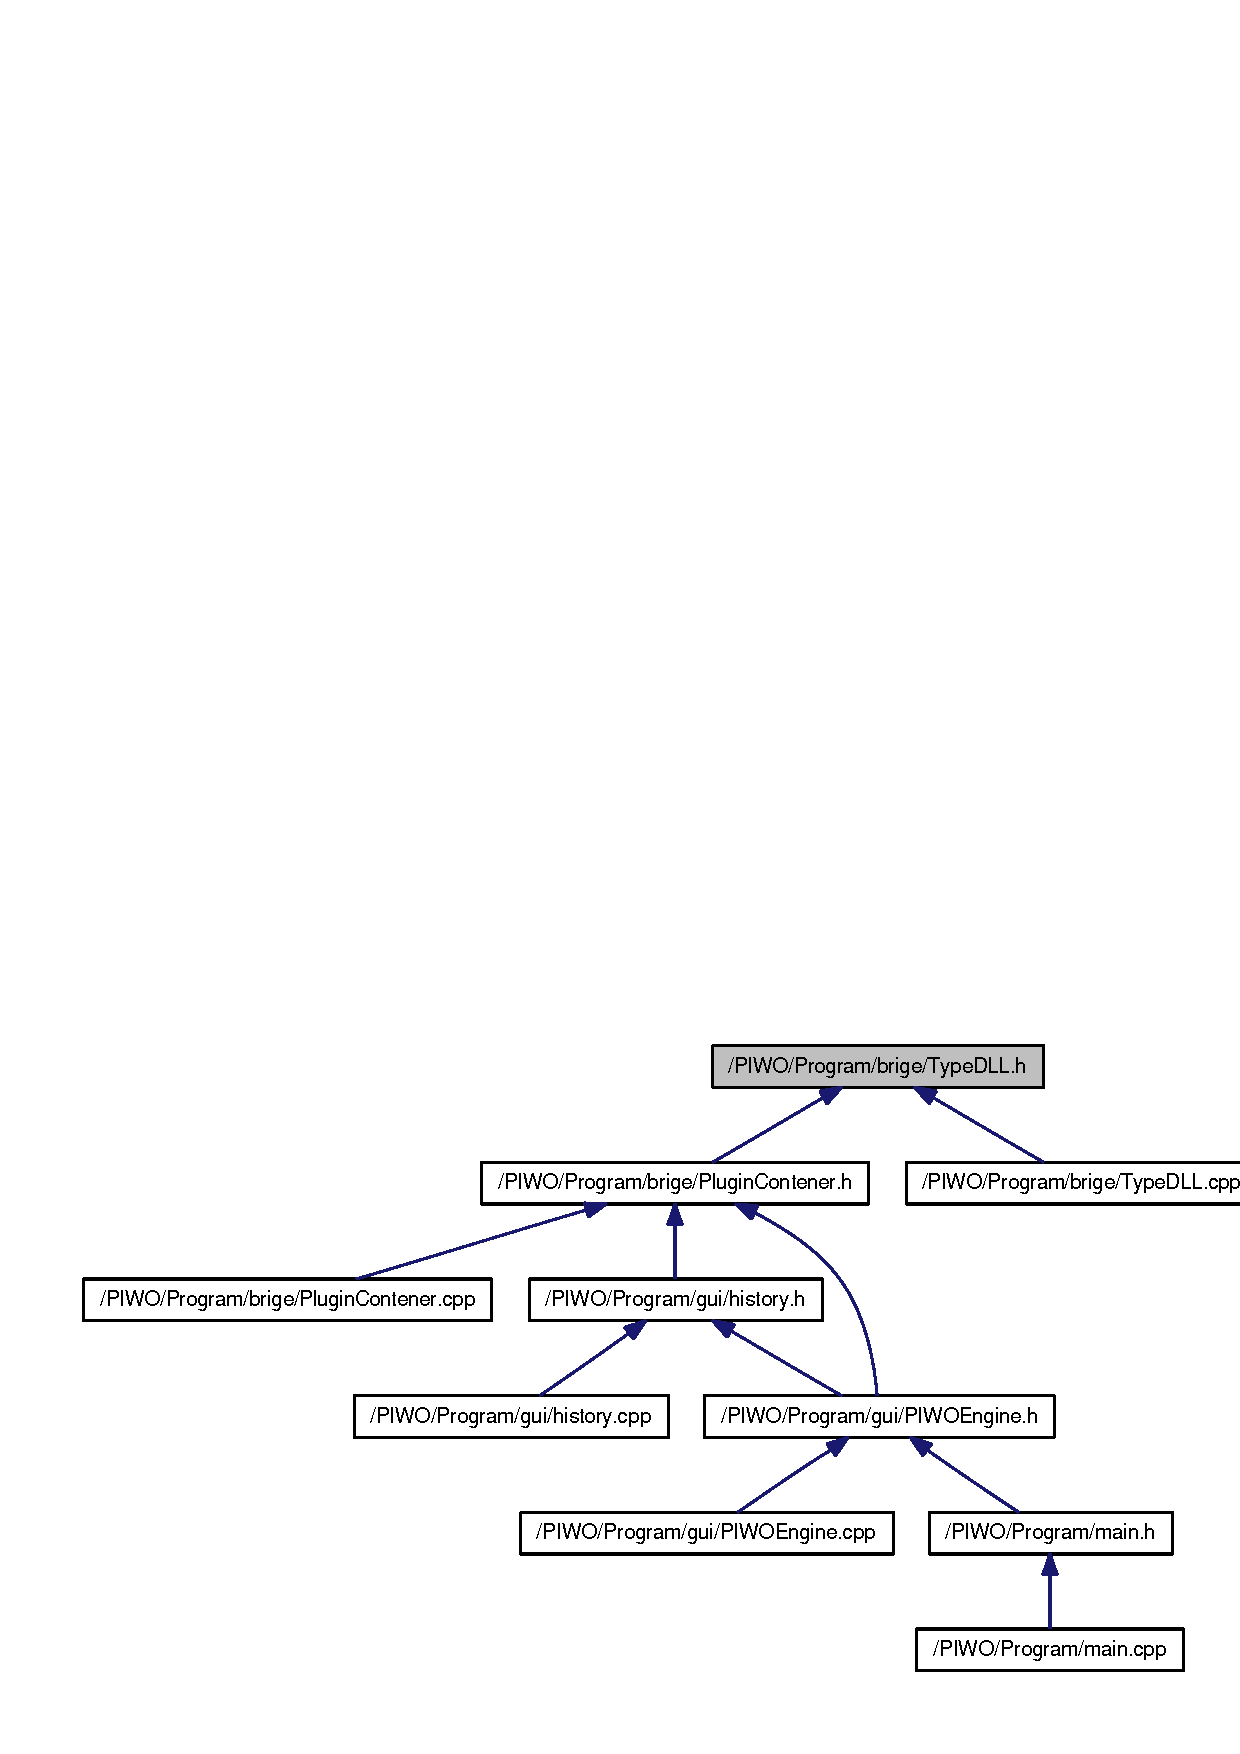
\includegraphics[width=303pt]{TypeDLL_8h__dep__incl}
\end{center}
\end{figure}
\subsection*{Classes}
\begin{CompactItemize}
\item 
class \hyperlink{classTypeDLL}{TypeDLL}
\end{CompactItemize}
\subsection*{Typedefs}
\begin{CompactItemize}
\item 
typedef TFrame $\ast$\_\-\_\-stdcall $\ast$ \hyperlink{TypeDLL_8h_e3b92b079373f3c0fae8106774b2c686}{TypeDLL\_\-show} (TWinControl $\ast$, \hyperlink{classTypeConfig}{TypeConfig} $\ast$)
\end{CompactItemize}
\subsection*{Functions}
\begin{CompactItemize}
\item 
typedef \hyperlink{TypeDLL_8h_359e052ece9c3760077088d1f98eb116}{bool} (\_\-\_\-stdcall $\ast$TypeDLL\_\-isValid)(\hyperlink{classTypeConfig}{TypeConfig} $\ast$)
\item 
typedef \hyperlink{TypeDLL_8h_330e37e6aac2a4a7bd3b303d1ddd71d6}{AnsiString} (\_\-\_\-stdcall $\ast$TypeDLL\_\-getType)()
\end{CompactItemize}


\subsection{Typedef Documentation}
\hypertarget{TypeDLL_8h_e3b92b079373f3c0fae8106774b2c686}{
\index{TypeDLL.h@{TypeDLL.h}!TypeDLL\_\-show@{TypeDLL\_\-show}}
\index{TypeDLL\_\-show@{TypeDLL\_\-show}!TypeDLL.h@{TypeDLL.h}}
\subsubsection[TypeDLL\_\-show]{\setlength{\rightskip}{0pt plus 5cm}typedef TFrame$\ast$ \_\-\_\-stdcall$\ast$ {\bf TypeDLL\_\-show}(TWinControl $\ast$, {\bf TypeConfig} $\ast$)}}
\label{TypeDLL_8h_e3b92b079373f3c0fae8106774b2c686}




Definition at line 12 of file TypeDLL.h.

\subsection{Function Documentation}
\hypertarget{TypeDLL_8h_330e37e6aac2a4a7bd3b303d1ddd71d6}{
\index{TypeDLL.h@{TypeDLL.h}!AnsiString@{AnsiString}}
\index{AnsiString@{AnsiString}!TypeDLL.h@{TypeDLL.h}}
\subsubsection[AnsiString]{\setlength{\rightskip}{0pt plus 5cm}typedef AnsiString (\_\-\_\-stdcall $\ast$ {\em TypeDLL\_\-getType})}}
\label{TypeDLL_8h_330e37e6aac2a4a7bd3b303d1ddd71d6}


\hypertarget{TypeDLL_8h_359e052ece9c3760077088d1f98eb116}{
\index{TypeDLL.h@{TypeDLL.h}!bool@{bool}}
\index{bool@{bool}!TypeDLL.h@{TypeDLL.h}}
\subsubsection[bool]{\setlength{\rightskip}{0pt plus 5cm}typedef bool (\_\-\_\-stdcall $\ast$ {\em TypeDLL\_\-isValid})}}
\label{TypeDLL_8h_359e052ece9c3760077088d1f98eb116}



\hypertarget{Block_8cpp}{
\section{/PIWO/Program/engine/Block.cpp File Reference}
\label{Block_8cpp}\index{/PIWO/Program/engine/Block.cpp@{/PIWO/Program/engine/Block.cpp}}
}
{\tt \#include \char`\"{}Block.h\char`\"{}}\par


Include dependency graph for Block.cpp:\nopagebreak
\begin{figure}[H]
\begin{center}
\leavevmode
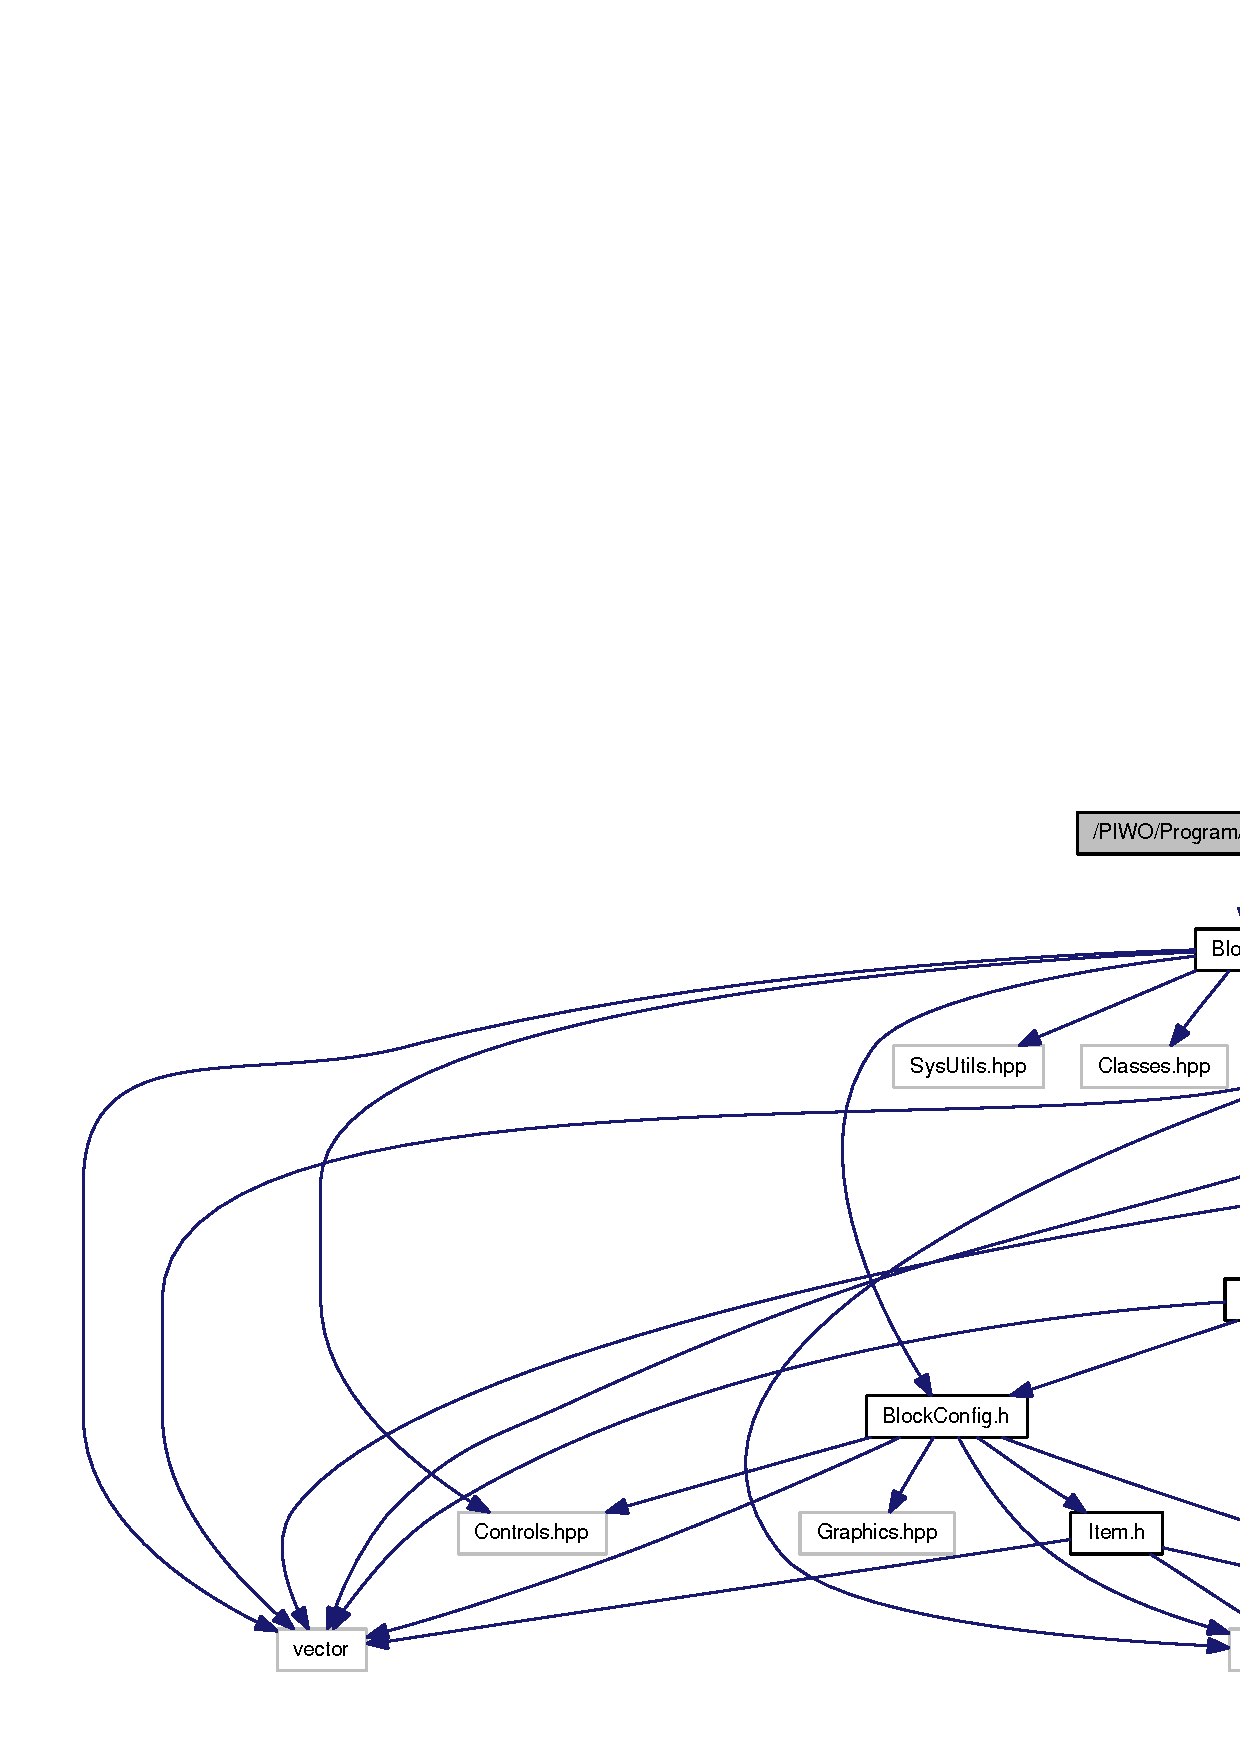
\includegraphics[width=420pt]{Block_8cpp__incl}
\end{center}
\end{figure}

\hypertarget{Block_8h}{
\section{/PIWO/Program/engine/Block.h File Reference}
\label{Block_8h}\index{/PIWO/Program/engine/Block.h@{/PIWO/Program/engine/Block.h}}
}
{\tt \#include $<$System.hpp$>$}\par
{\tt \#include $<$vector$>$}\par
{\tt \#include $<$exception$>$}\par
{\tt \#include $<$SysUtils.hpp$>$}\par
{\tt \#include $<$Classes.hpp$>$}\par
{\tt \#include $<$Controls.hpp$>$}\par
{\tt \#include $<$Forms.hpp$>$}\par
{\tt \#include \char`\"{}BlockConfig.h\char`\"{}}\par
{\tt \#include \char`\"{}BlockInput.h\char`\"{}}\par
{\tt \#include \char`\"{}BlockOutput.h\char`\"{}}\par


Include dependency graph for Block.h:\nopagebreak
\begin{figure}[H]
\begin{center}
\leavevmode
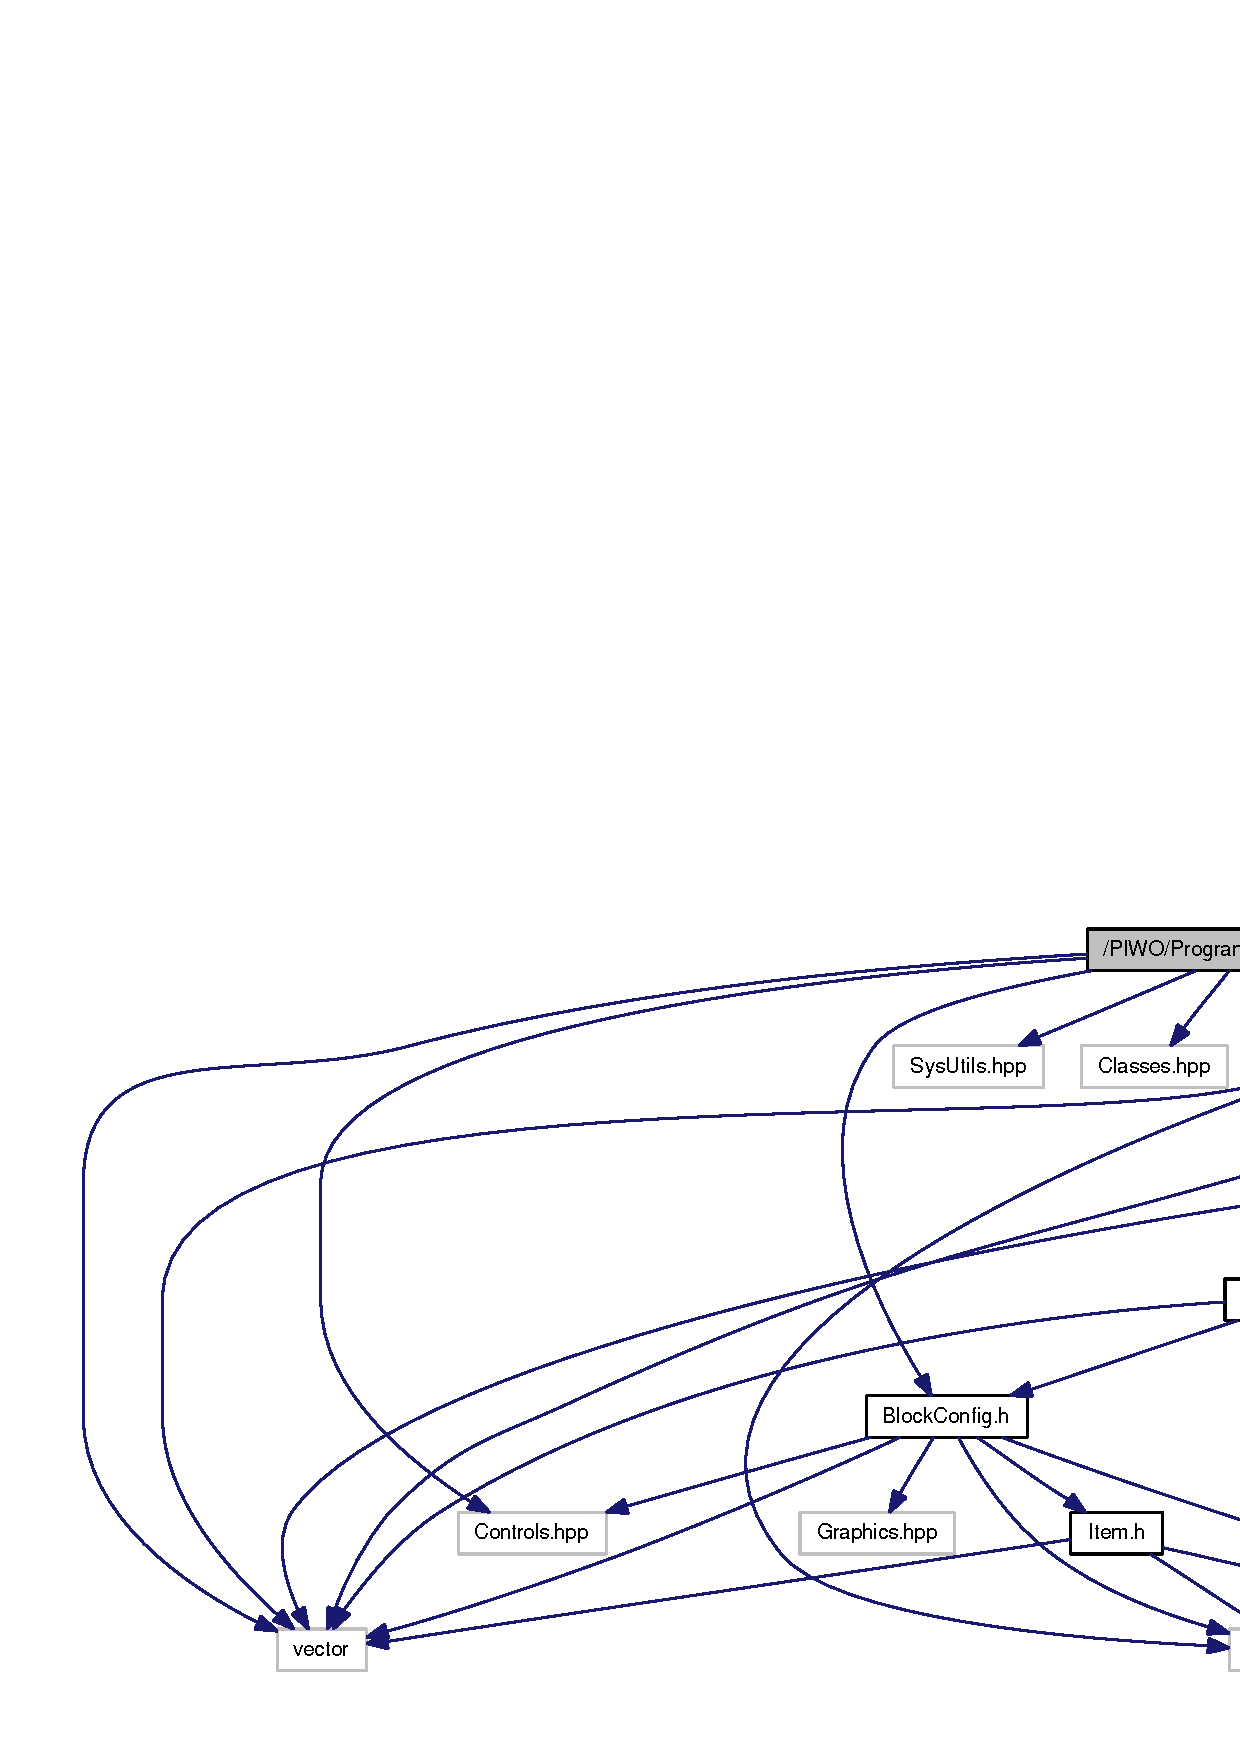
\includegraphics[width=420pt]{Block_8h__incl}
\end{center}
\end{figure}


This graph shows which files directly or indirectly include this file:\nopagebreak
\begin{figure}[H]
\begin{center}
\leavevmode
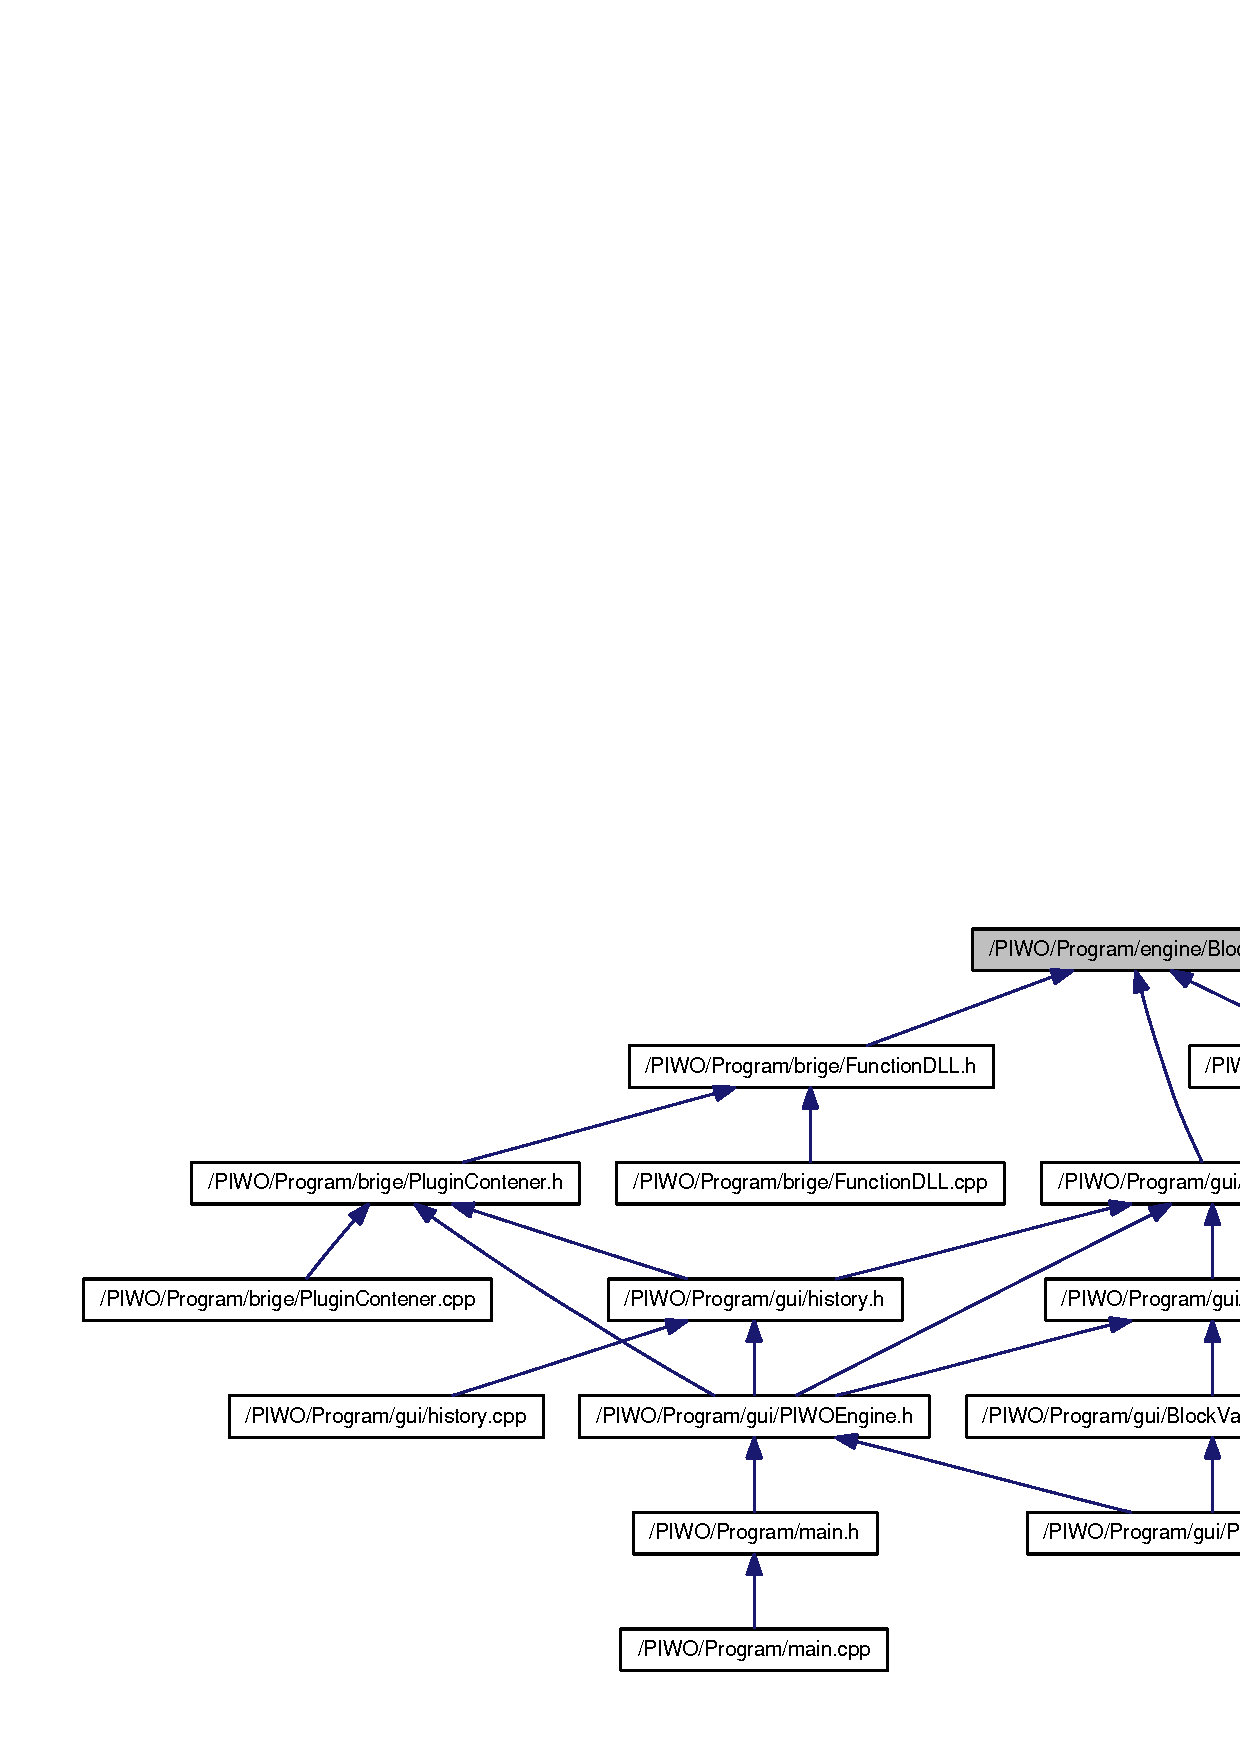
\includegraphics[width=420pt]{Block_8h__dep__incl}
\end{center}
\end{figure}
\subsection*{Classes}
\begin{CompactItemize}
\item 
class \hyperlink{classBlock}{Block}
\end{CompactItemize}

\hypertarget{BlockConfig_8cpp}{
\section{/PIWO/Program/engine/BlockConfig.cpp File Reference}
\label{BlockConfig_8cpp}\index{/PIWO/Program/engine/BlockConfig.cpp@{/PIWO/Program/engine/BlockConfig.cpp}}
}
{\tt \#include \char`\"{}BlockConfig.h\char`\"{}}\par


Include dependency graph for BlockConfig.cpp:\nopagebreak
\begin{figure}[H]
\begin{center}
\leavevmode
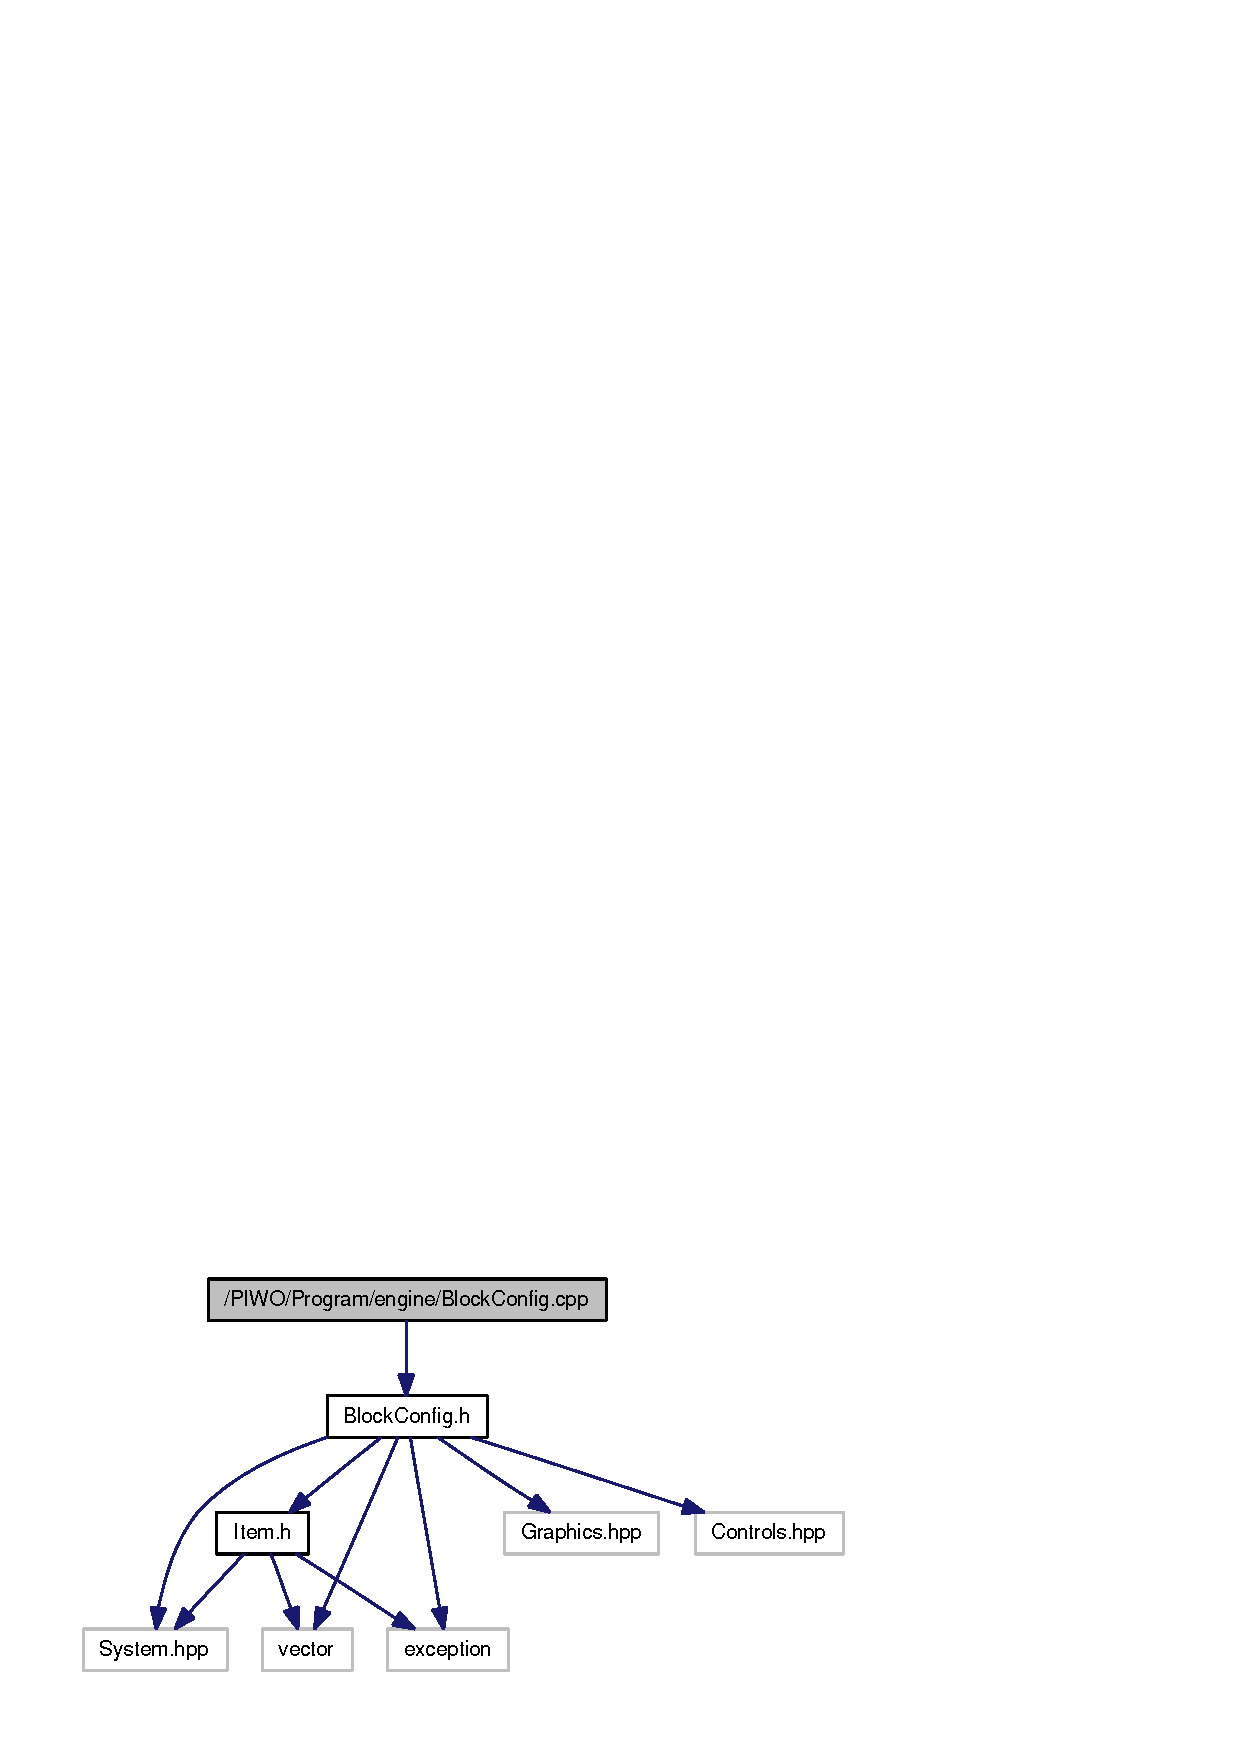
\includegraphics[width=204pt]{BlockConfig_8cpp__incl}
\end{center}
\end{figure}

\hypertarget{BlockConfig_8h}{
\section{/PIWO/Program/engine/BlockConfig.h File Reference}
\label{BlockConfig_8h}\index{/PIWO/Program/engine/BlockConfig.h@{/PIWO/Program/engine/BlockConfig.h}}
}
{\tt \#include $<$System.hpp$>$}\par
{\tt \#include $<$Graphics.hpp$>$}\par
{\tt \#include $<$Controls.hpp$>$}\par
{\tt \#include $<$vector$>$}\par
{\tt \#include $<$exception$>$}\par
{\tt \#include \char`\"{}Item.h\char`\"{}}\par


Include dependency graph for BlockConfig.h:\nopagebreak
\begin{figure}[H]
\begin{center}
\leavevmode
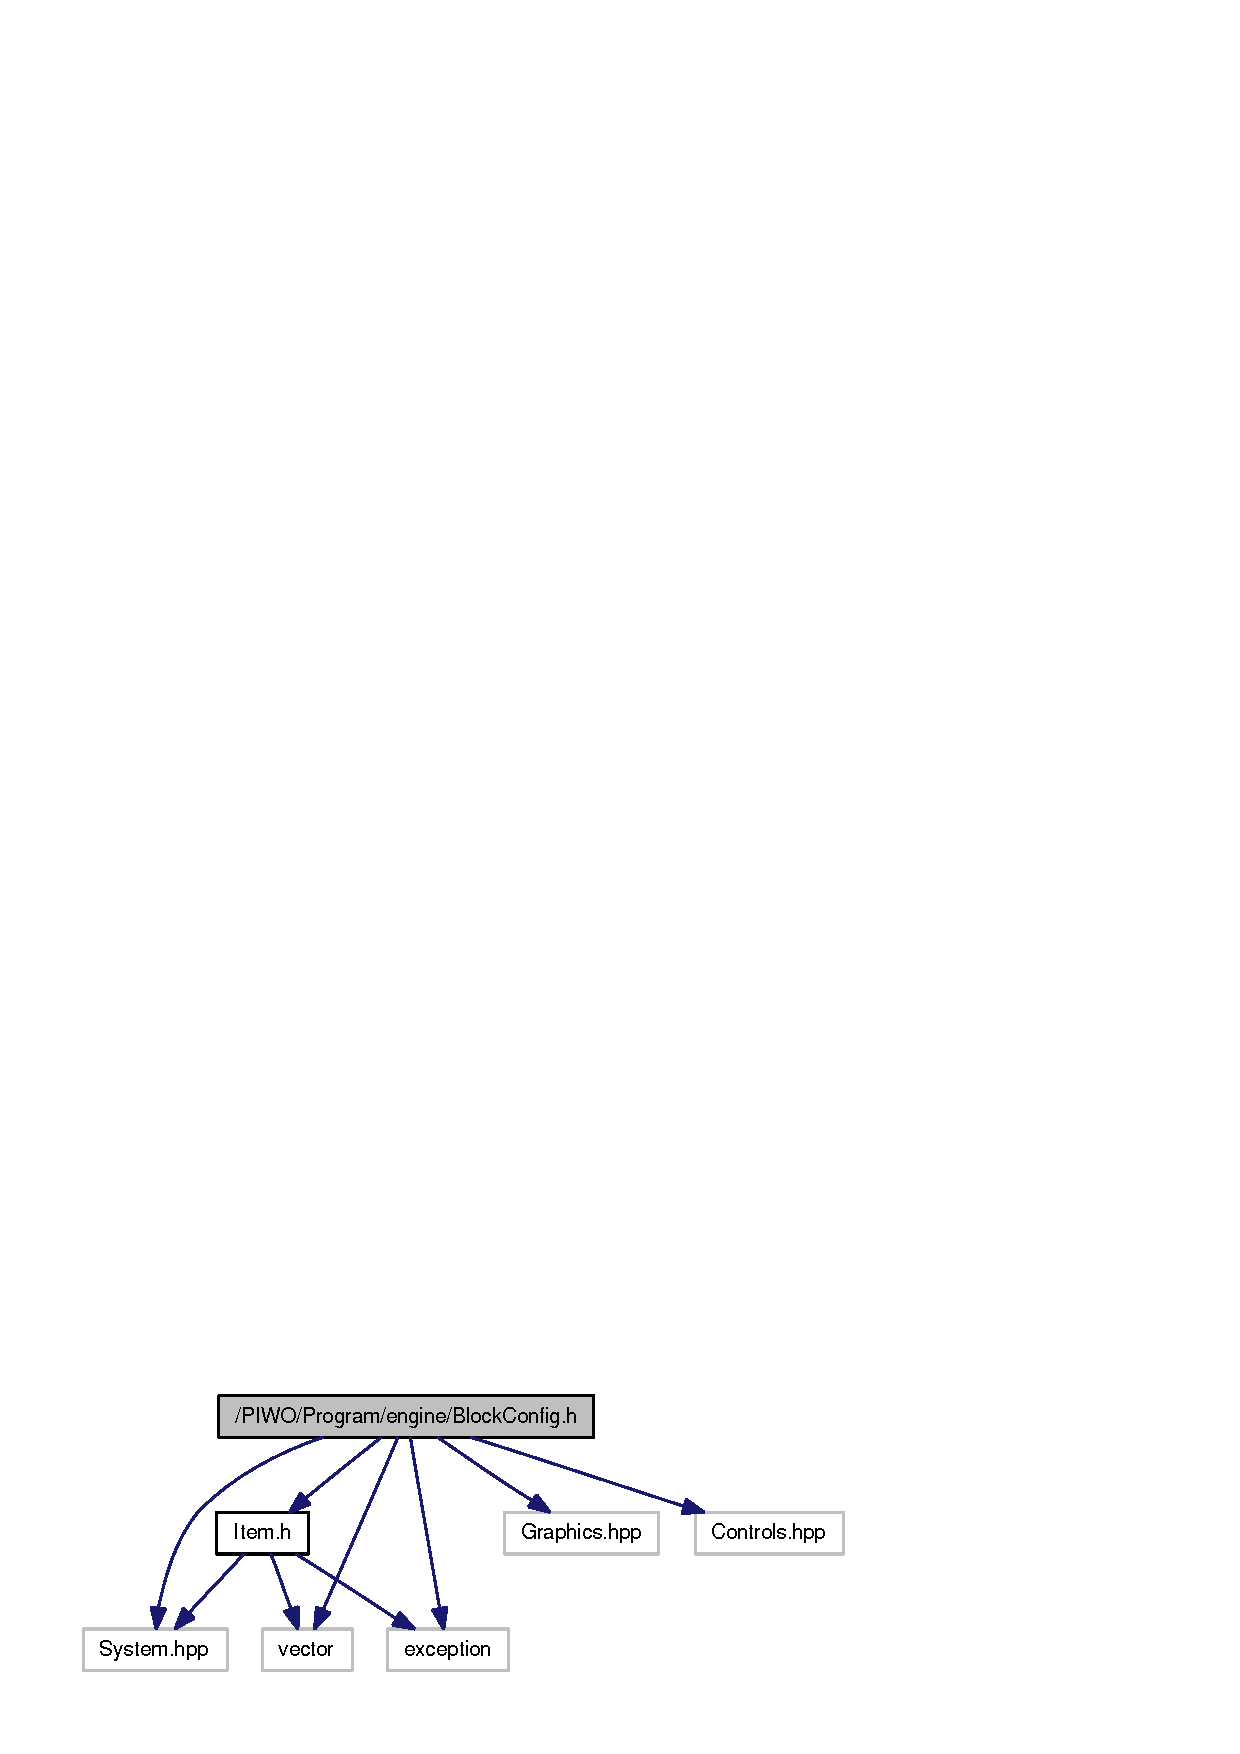
\includegraphics[width=204pt]{BlockConfig_8h__incl}
\end{center}
\end{figure}


This graph shows which files directly or indirectly include this file:\nopagebreak
\begin{figure}[H]
\begin{center}
\leavevmode
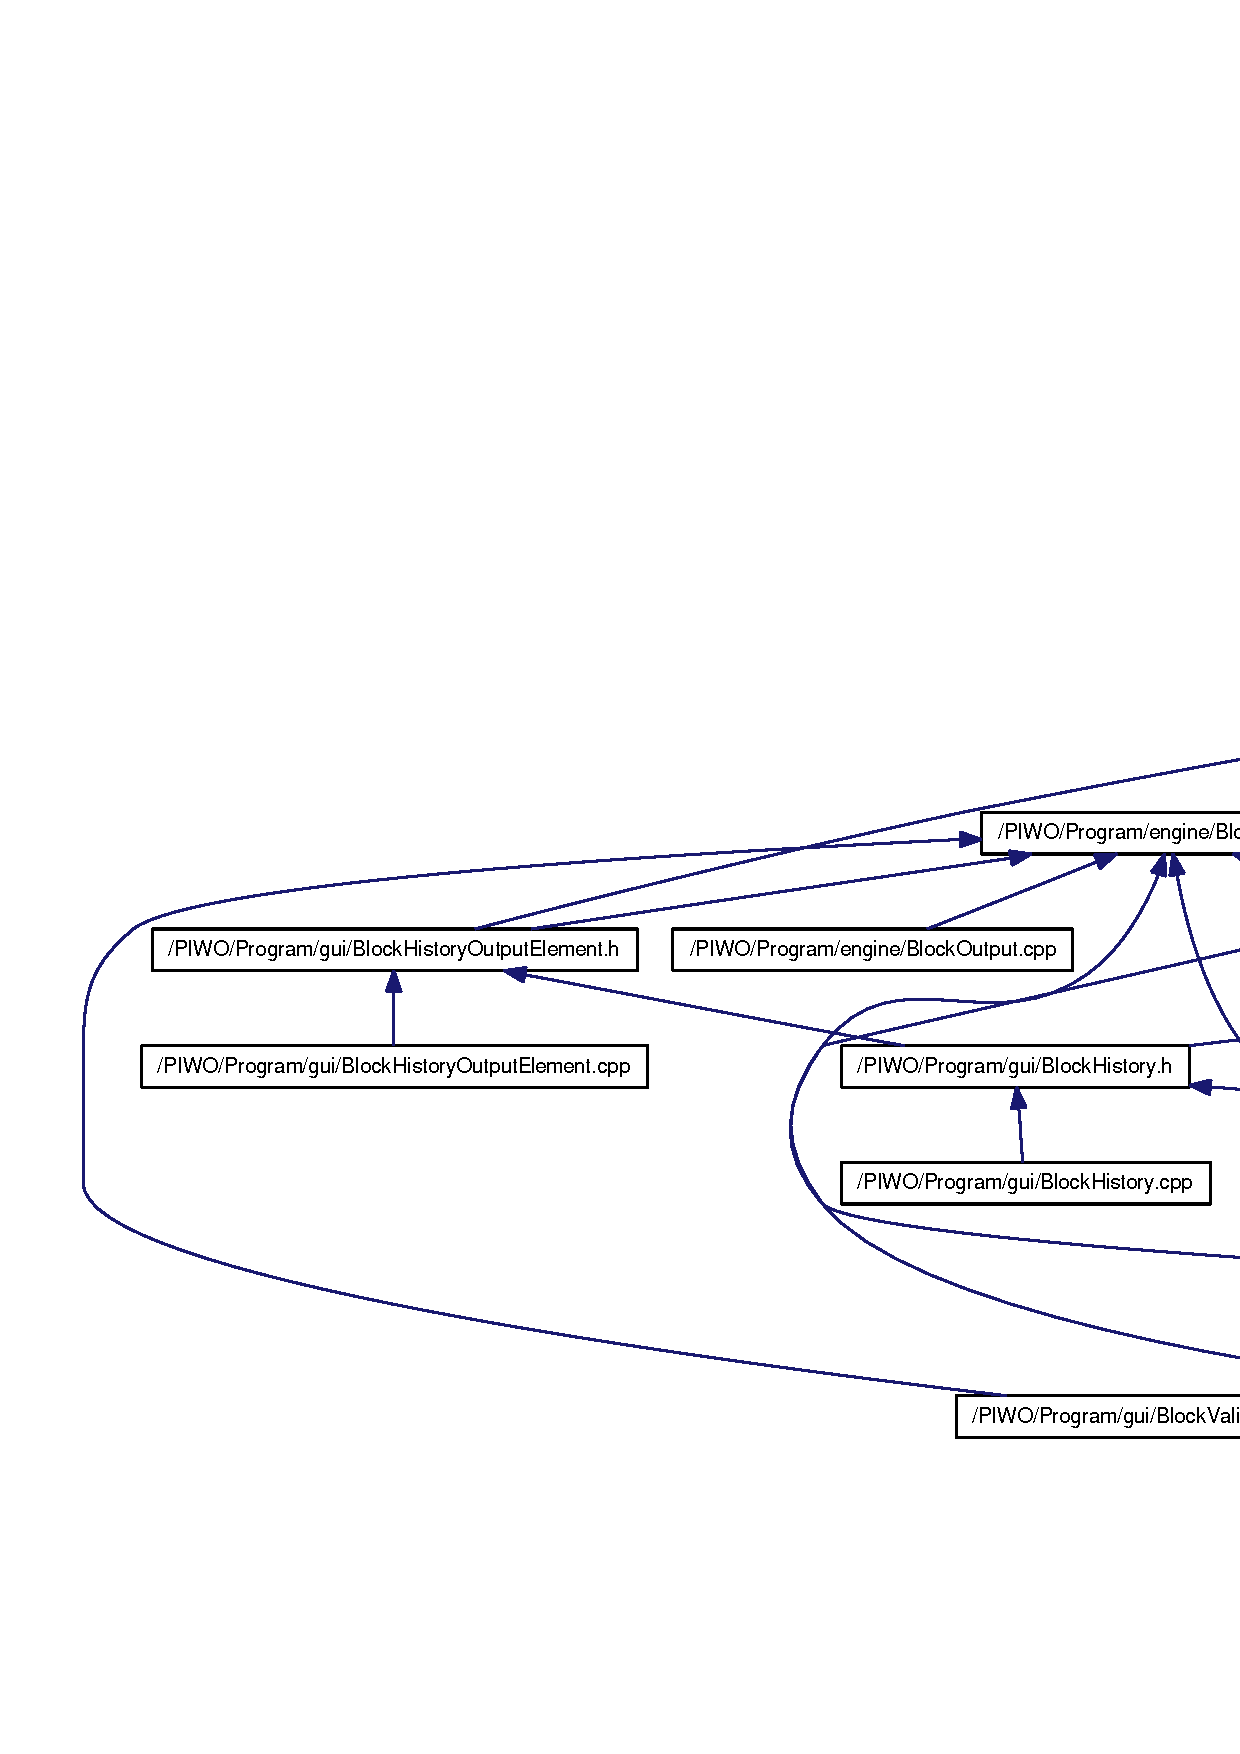
\includegraphics[width=420pt]{BlockConfig_8h__dep__incl}
\end{center}
\end{figure}
\subsection*{Classes}
\begin{CompactItemize}
\item 
class \hyperlink{classBlockConfig}{BlockConfig}
\end{CompactItemize}

\hypertarget{BlockElement_8cpp}{
\section{/PIWO/Program/engine/BlockElement.cpp File Reference}
\label{BlockElement_8cpp}\index{/PIWO/Program/engine/BlockElement.cpp@{/PIWO/Program/engine/BlockElement.cpp}}
}
{\tt \#include \char`\"{}BlockElement.h\char`\"{}}\par


Include dependency graph for BlockElement.cpp:\nopagebreak
\begin{figure}[H]
\begin{center}
\leavevmode
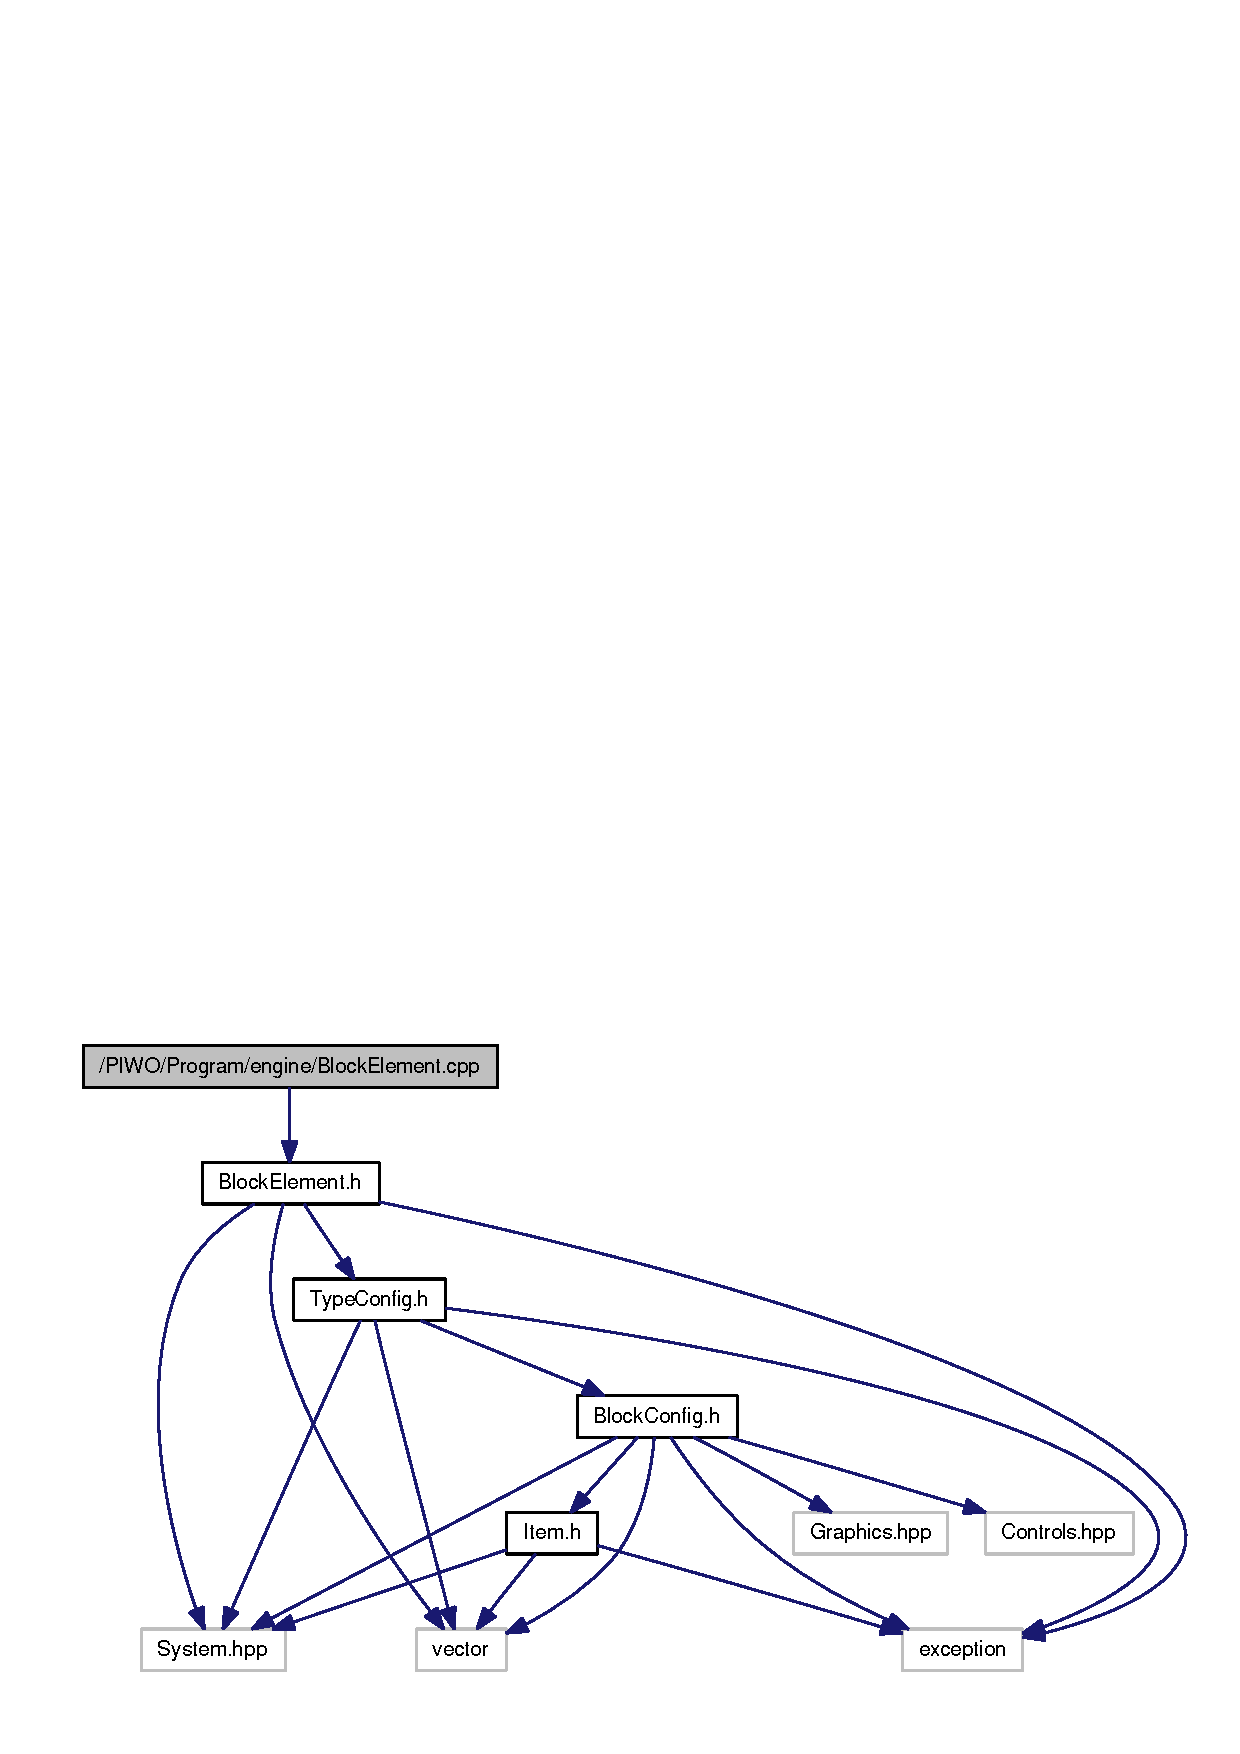
\includegraphics[width=293pt]{BlockElement_8cpp__incl}
\end{center}
\end{figure}

\hypertarget{BlockElement_8h}{
\section{/PIWO/Program/engine/BlockElement.h File Reference}
\label{BlockElement_8h}\index{/PIWO/Program/engine/BlockElement.h@{/PIWO/Program/engine/BlockElement.h}}
}
{\tt \#include $<$System.hpp$>$}\par
{\tt \#include $<$vector$>$}\par
{\tt \#include $<$exception$>$}\par
{\tt \#include \char`\"{}TypeConfig.h\char`\"{}}\par


Include dependency graph for BlockElement.h:\nopagebreak
\begin{figure}[H]
\begin{center}
\leavevmode
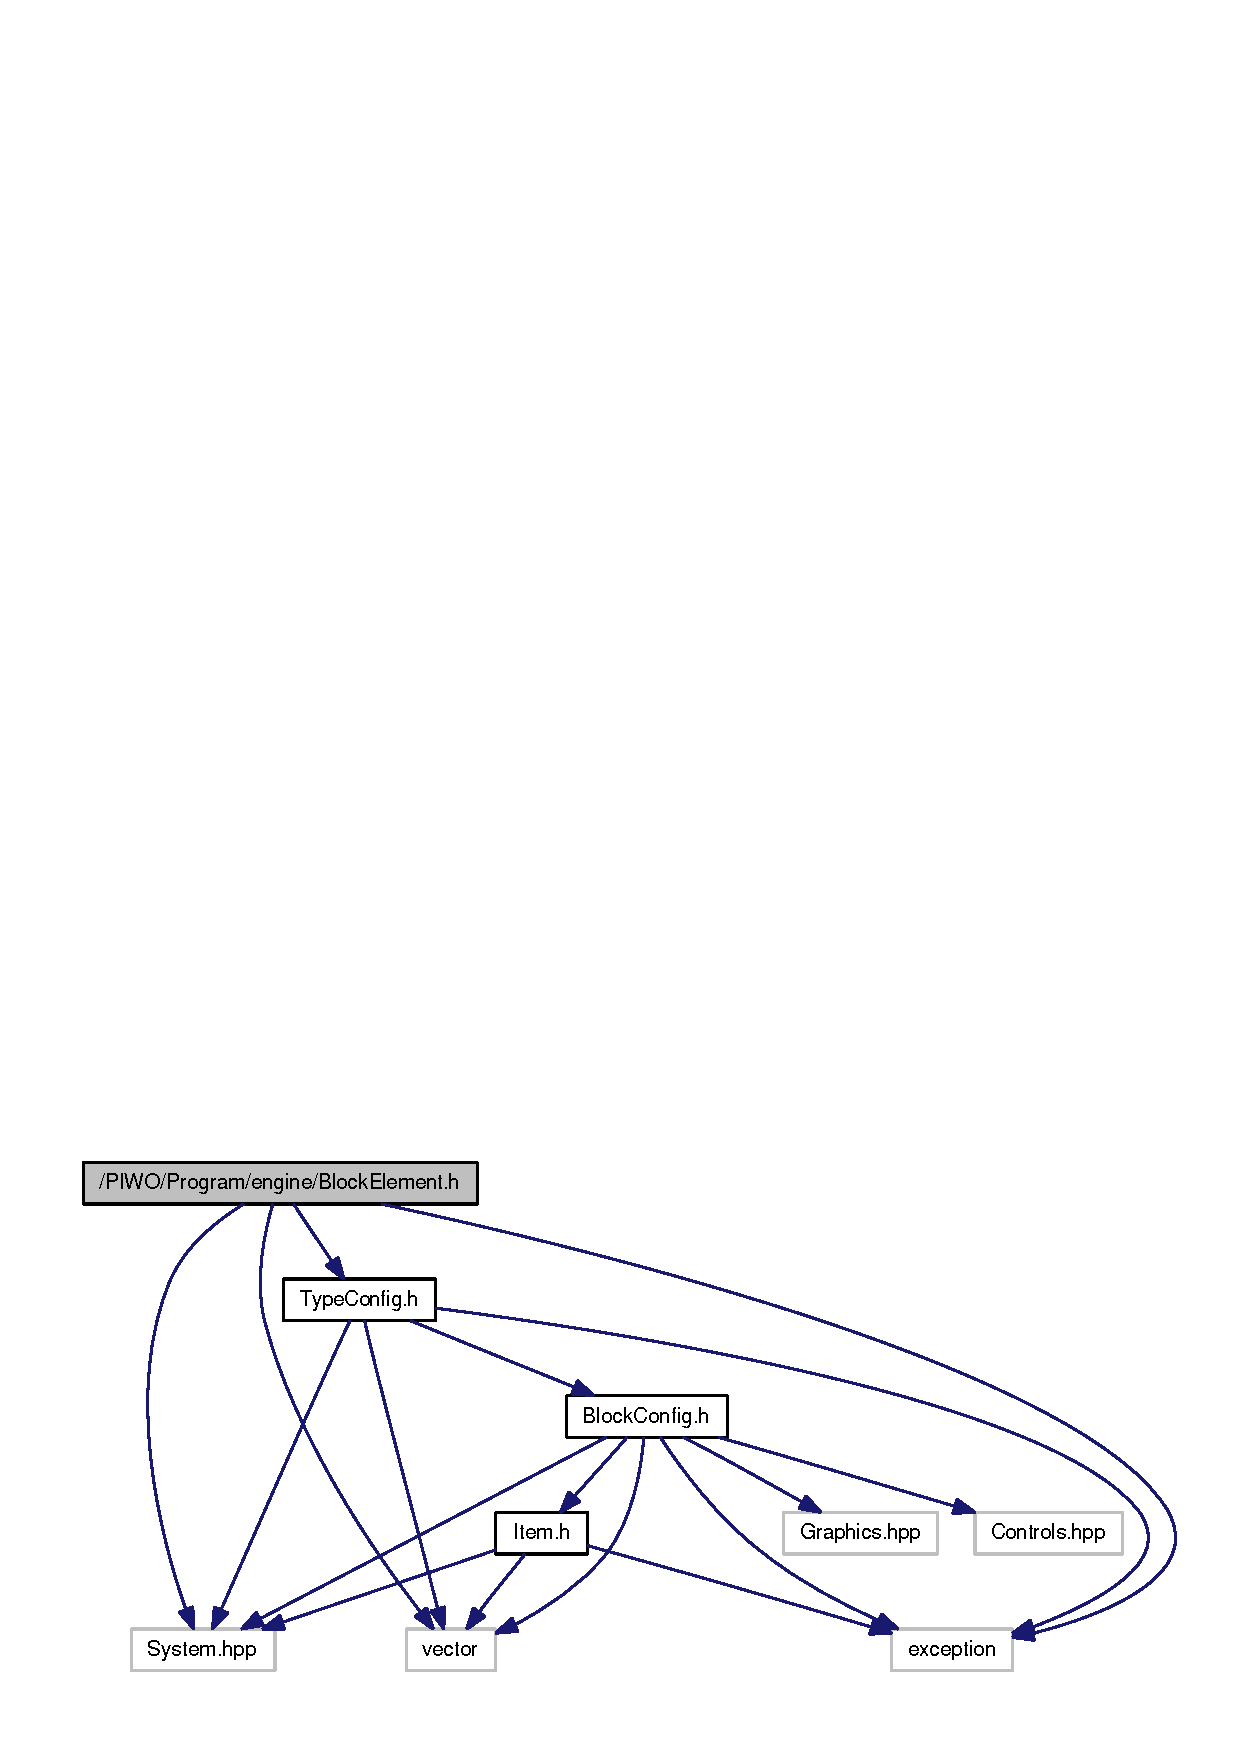
\includegraphics[width=290pt]{BlockElement_8h__incl}
\end{center}
\end{figure}


This graph shows which files directly or indirectly include this file:\nopagebreak
\begin{figure}[H]
\begin{center}
\leavevmode
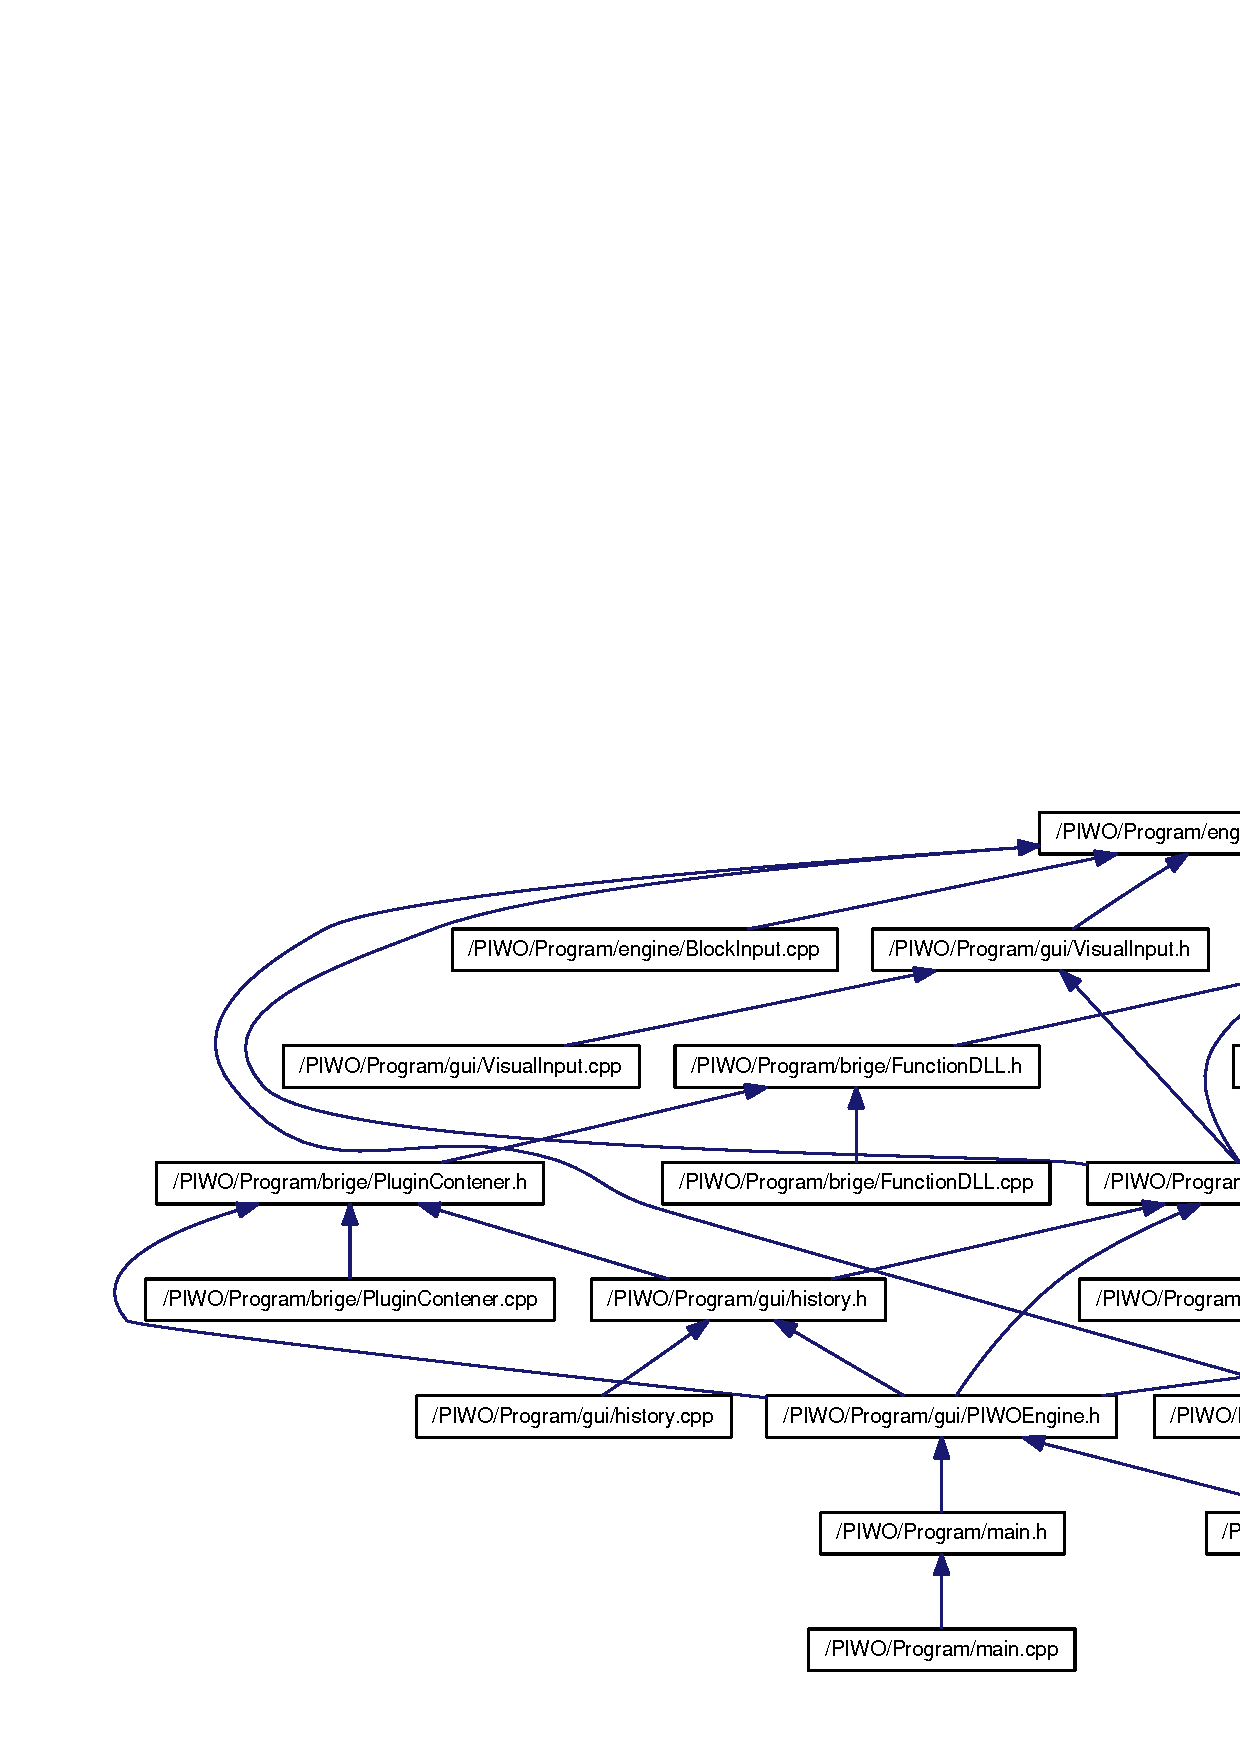
\includegraphics[width=420pt]{BlockElement_8h__dep__incl}
\end{center}
\end{figure}
\subsection*{Classes}
\begin{CompactItemize}
\item 
class \hyperlink{classBlockElement}{BlockElement}
\end{CompactItemize}

\hypertarget{BlockInput_8cpp}{
\section{/PIWO/Program/engine/BlockInput.cpp File Reference}
\label{BlockInput_8cpp}\index{/PIWO/Program/engine/BlockInput.cpp@{/PIWO/Program/engine/BlockInput.cpp}}
}
{\tt \#include \char`\"{}BlockInput.h\char`\"{}}\par


Include dependency graph for BlockInput.cpp:\nopagebreak
\begin{figure}[H]
\begin{center}
\leavevmode
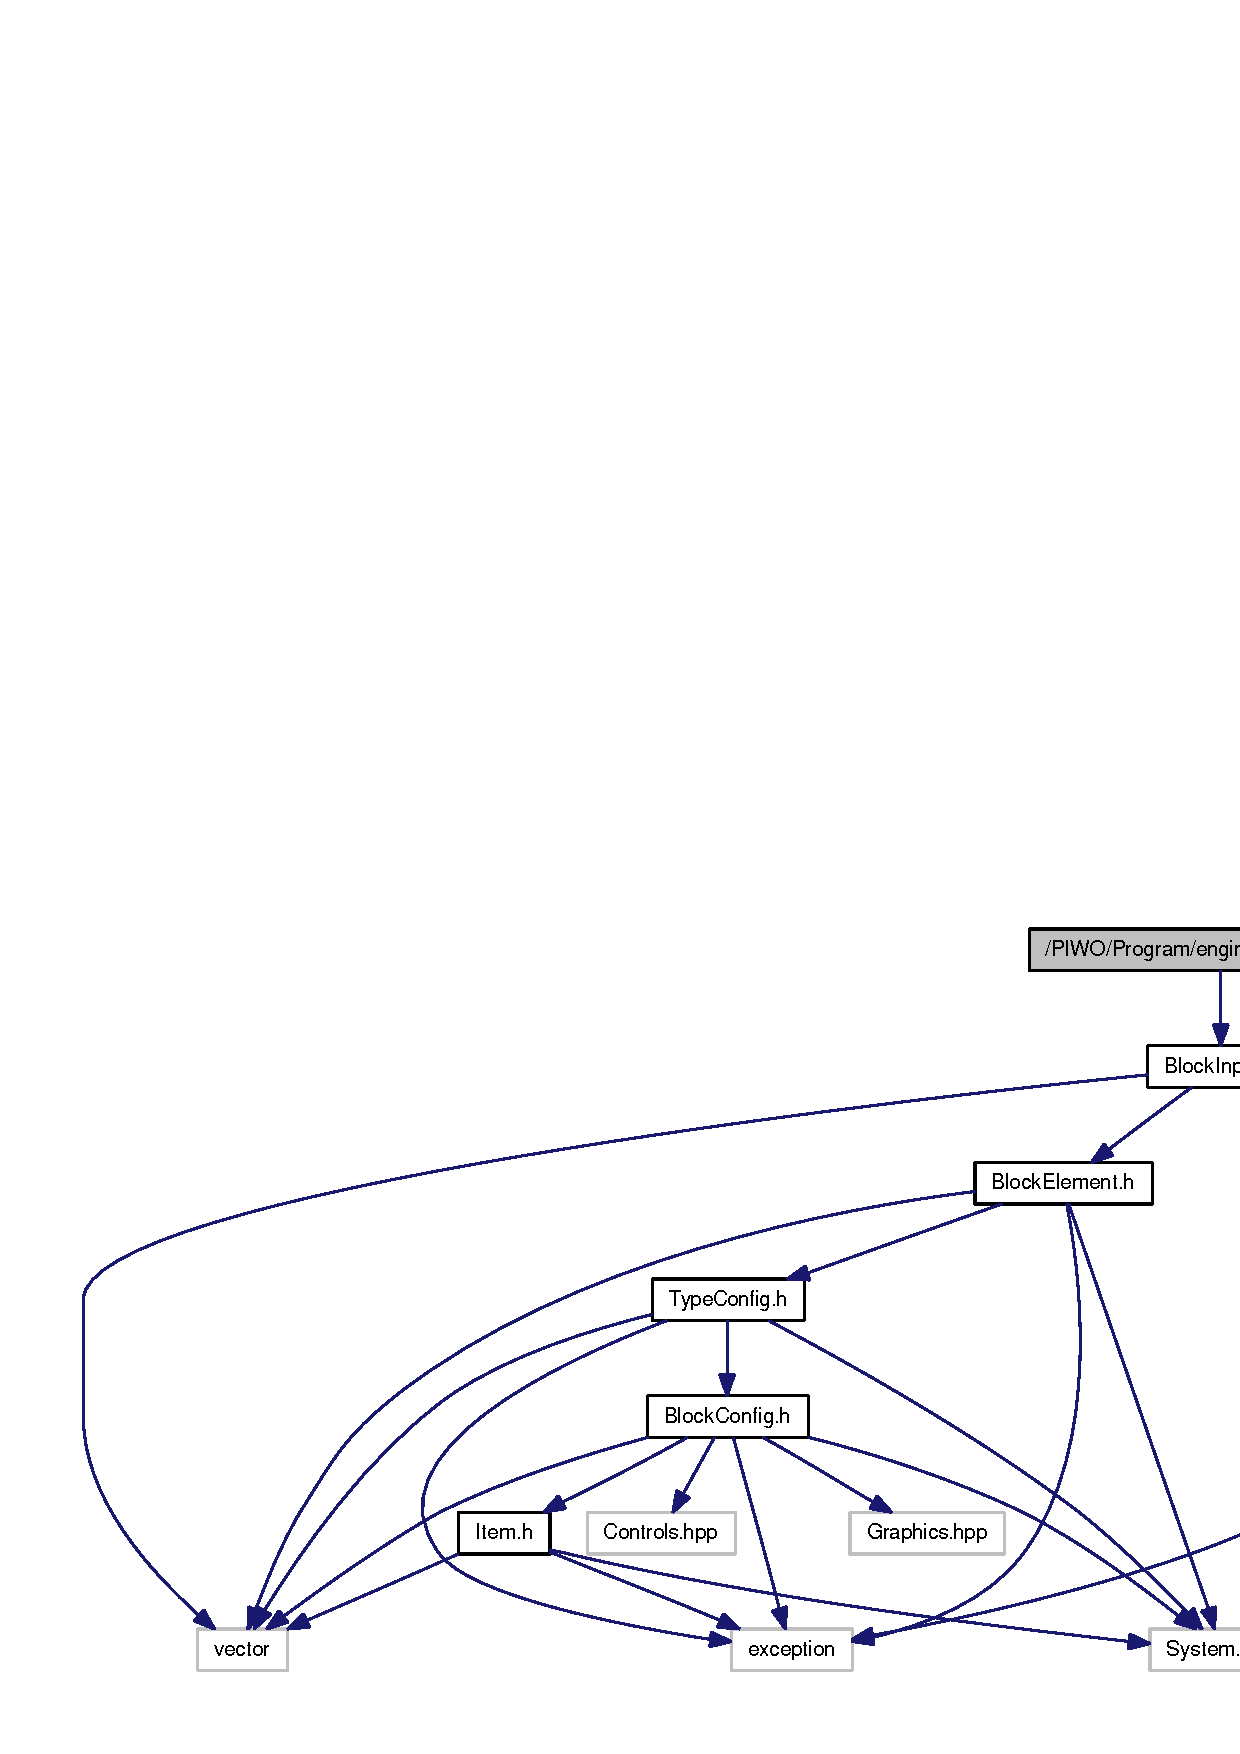
\includegraphics[width=352pt]{BlockInput_8cpp__incl}
\end{center}
\end{figure}

\hypertarget{BlockInput_8h}{
\section{/PIWO/Program/engine/BlockInput.h File Reference}
\label{BlockInput_8h}\index{/PIWO/Program/engine/BlockInput.h@{/PIWO/Program/engine/BlockInput.h}}
}
{\tt \#include $<$System.hpp$>$}\par
{\tt \#include $<$vector$>$}\par
{\tt \#include $<$exception$>$}\par
{\tt \#include \char`\"{}BlockElement.h\char`\"{}}\par


Include dependency graph for BlockInput.h:\nopagebreak
\begin{figure}[H]
\begin{center}
\leavevmode
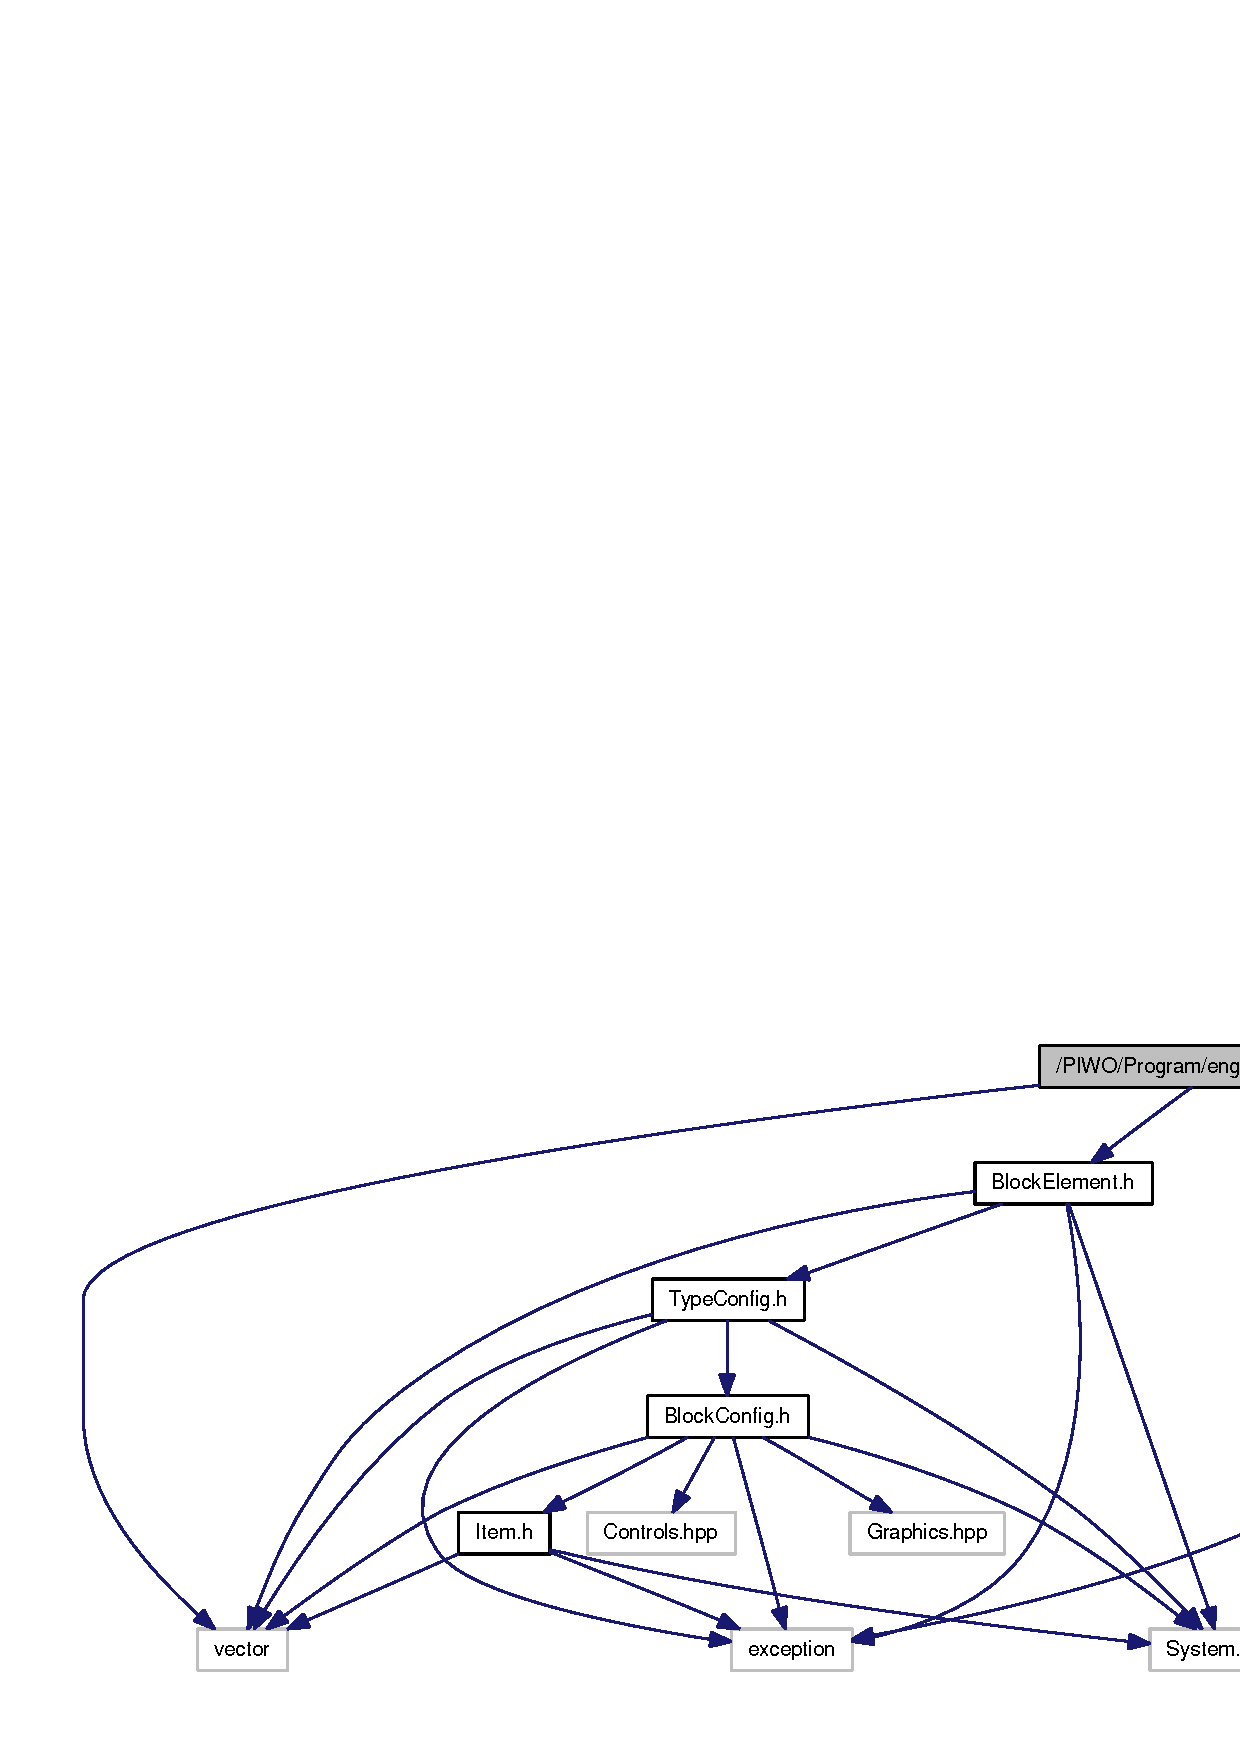
\includegraphics[width=352pt]{BlockInput_8h__incl}
\end{center}
\end{figure}


This graph shows which files directly or indirectly include this file:\nopagebreak
\begin{figure}[H]
\begin{center}
\leavevmode
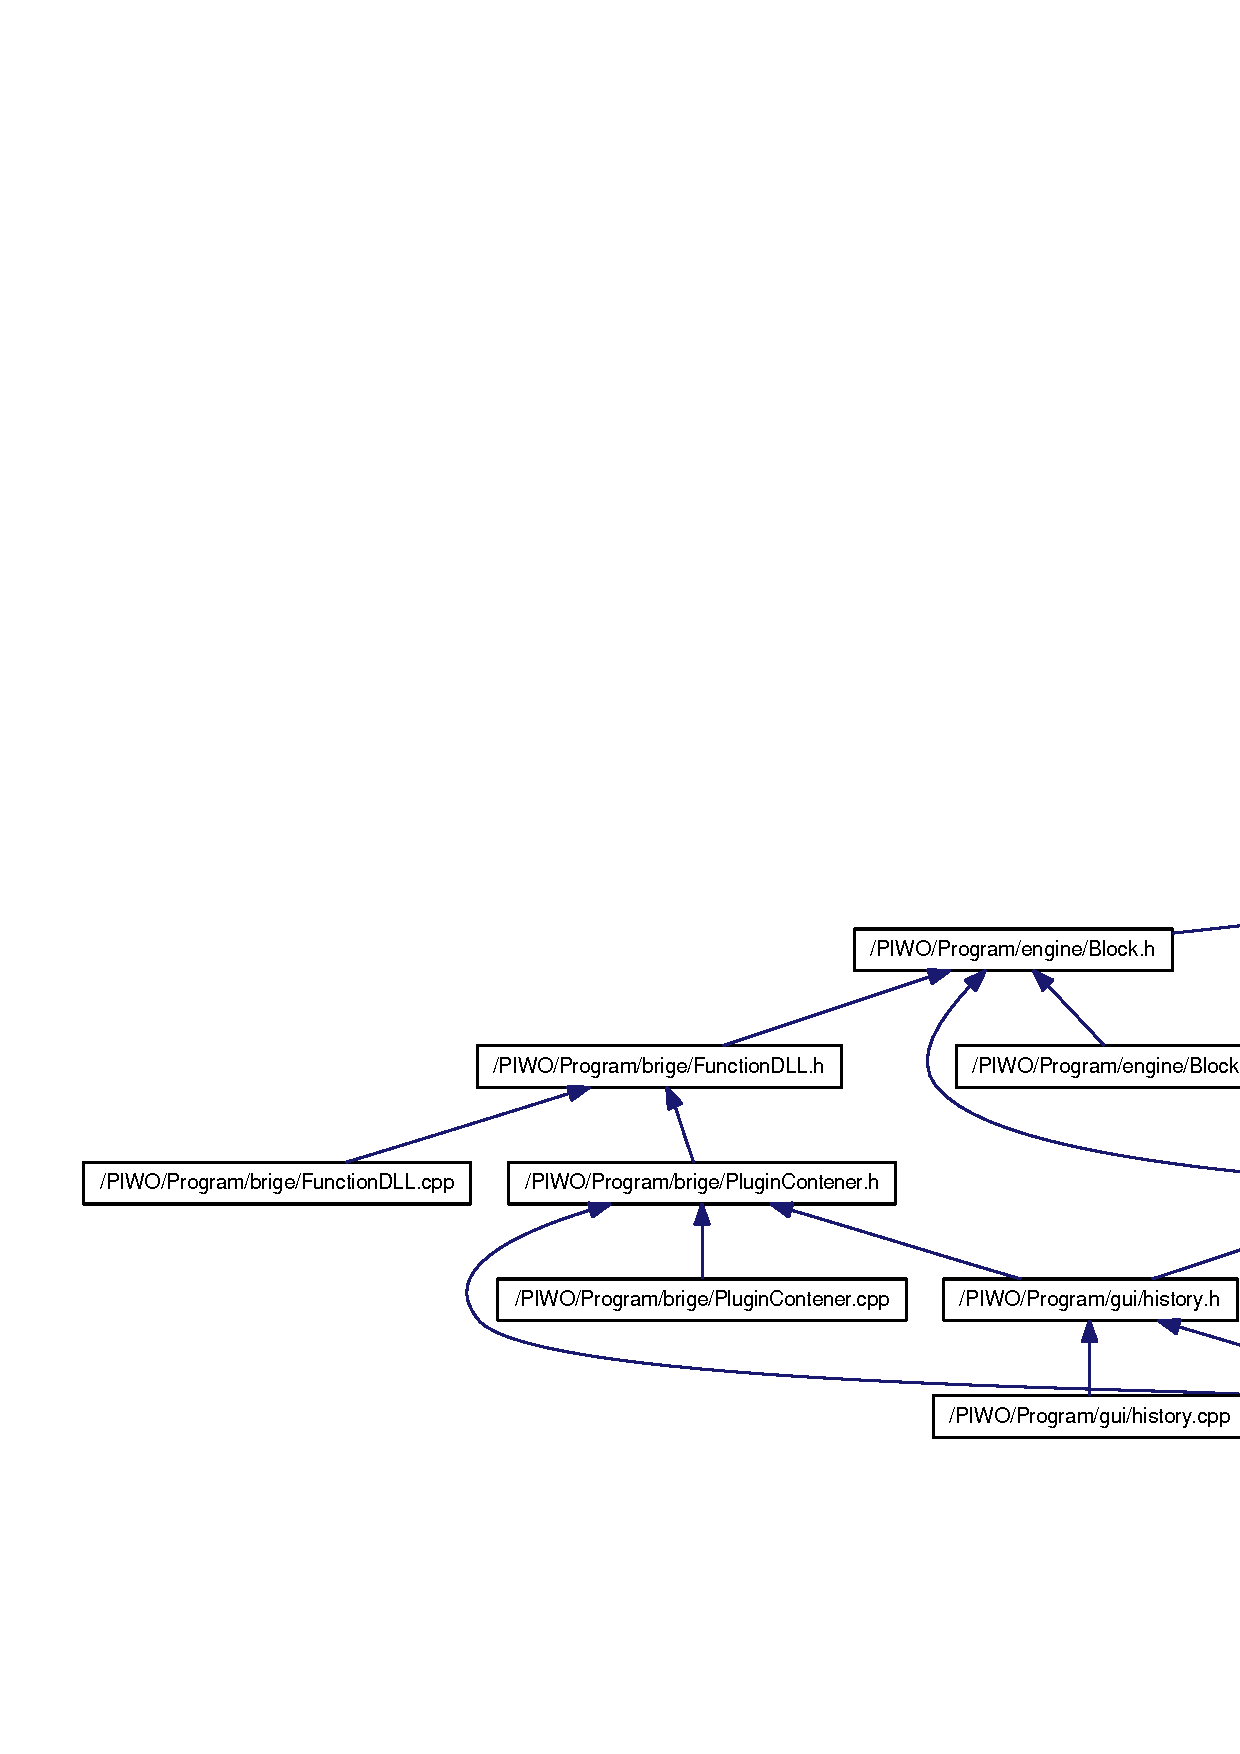
\includegraphics[width=420pt]{BlockInput_8h__dep__incl}
\end{center}
\end{figure}
\subsection*{Classes}
\begin{CompactItemize}
\item 
class \hyperlink{classBlockInput}{BlockInput}
\end{CompactItemize}

\hypertarget{BlockOutput_8cpp}{
\section{/PIWO/Program/engine/BlockOutput.cpp File Reference}
\label{BlockOutput_8cpp}\index{/PIWO/Program/engine/BlockOutput.cpp@{/PIWO/Program/engine/BlockOutput.cpp}}
}
{\tt \#include \char`\"{}BlockOutput.h\char`\"{}}\par


Include dependency graph for BlockOutput.cpp:\nopagebreak
\begin{figure}[H]
\begin{center}
\leavevmode
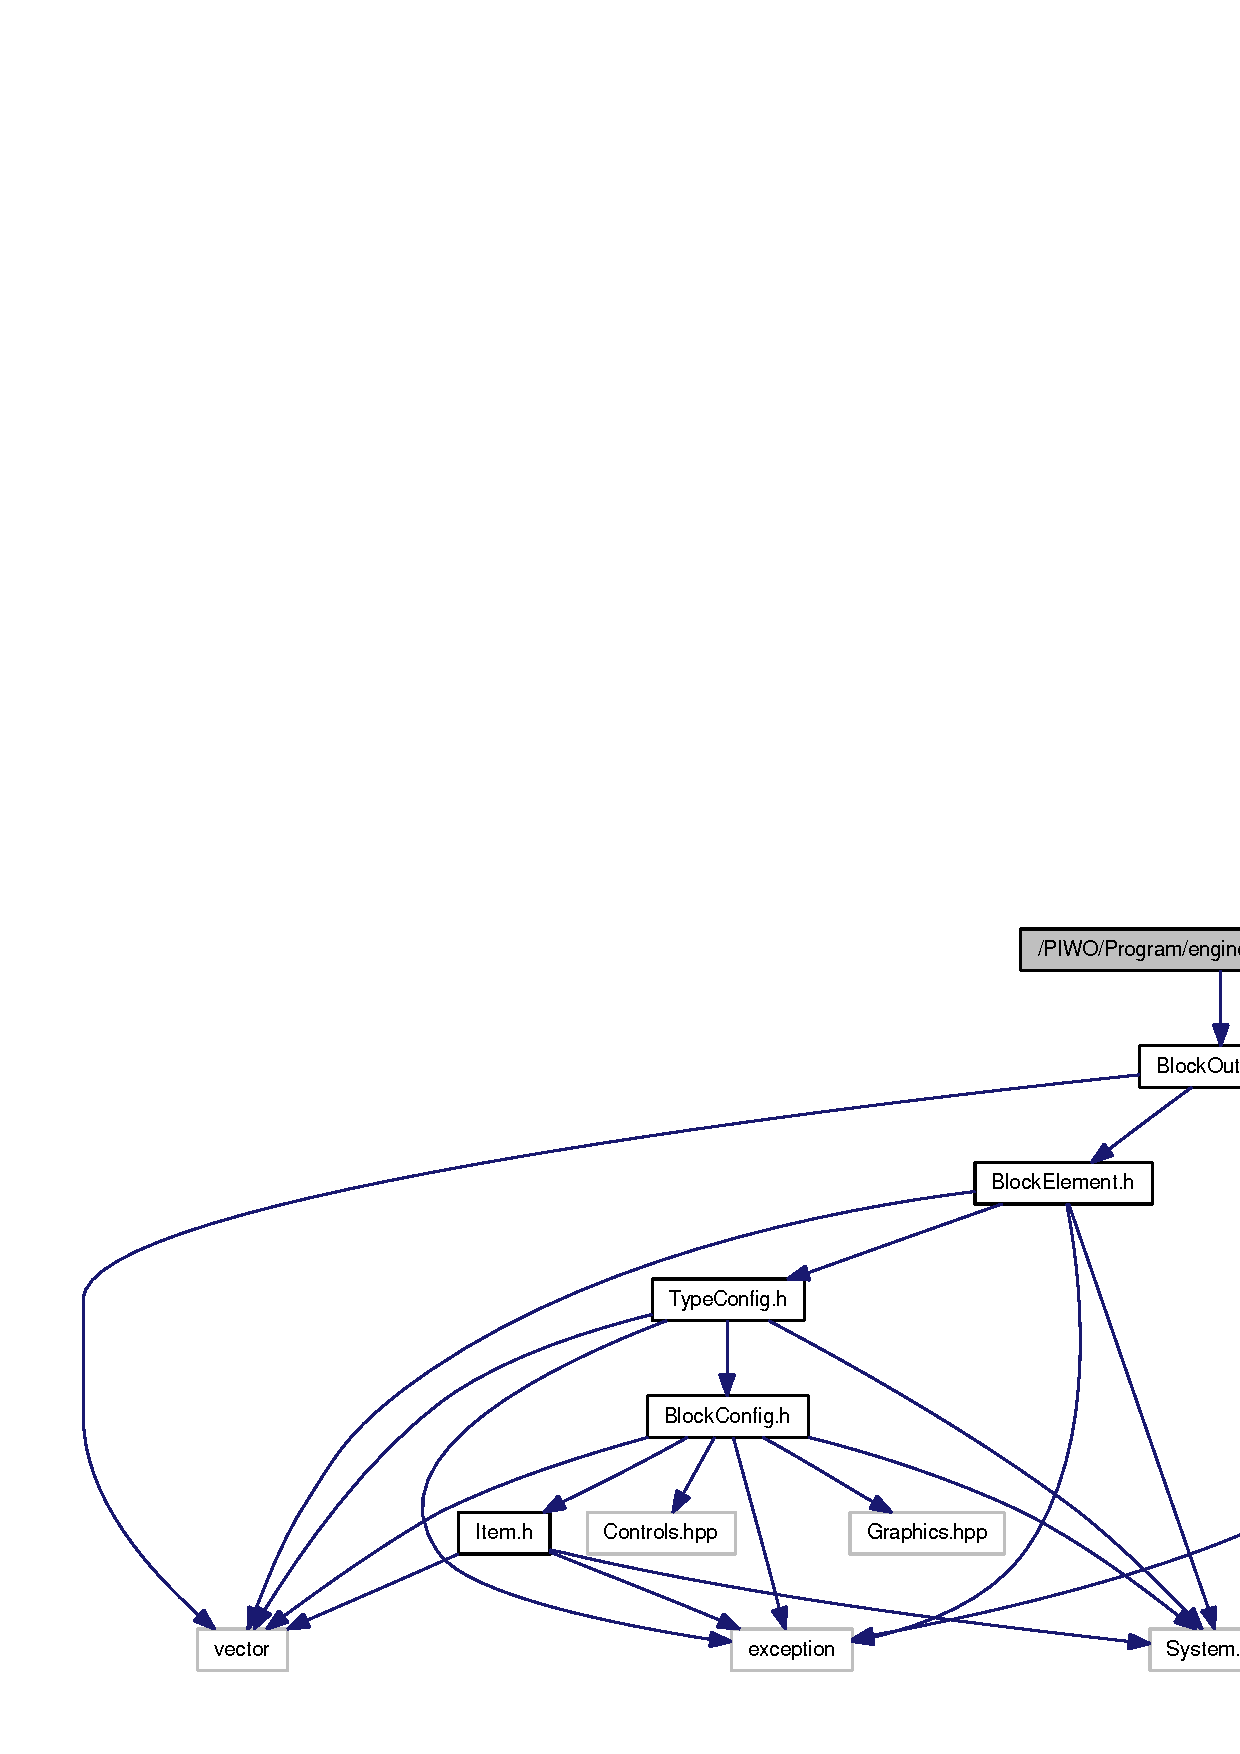
\includegraphics[width=352pt]{BlockOutput_8cpp__incl}
\end{center}
\end{figure}

\hypertarget{BlockOutput_8h}{
\section{/PIWO/Program/engine/BlockOutput.h File Reference}
\label{BlockOutput_8h}\index{/PIWO/Program/engine/BlockOutput.h@{/PIWO/Program/engine/BlockOutput.h}}
}
{\tt \#include $<$System.hpp$>$}\par
{\tt \#include $<$vector$>$}\par
{\tt \#include $<$exception$>$}\par
{\tt \#include \char`\"{}BlockElement.h\char`\"{}}\par


Include dependency graph for BlockOutput.h:\nopagebreak
\begin{figure}[H]
\begin{center}
\leavevmode
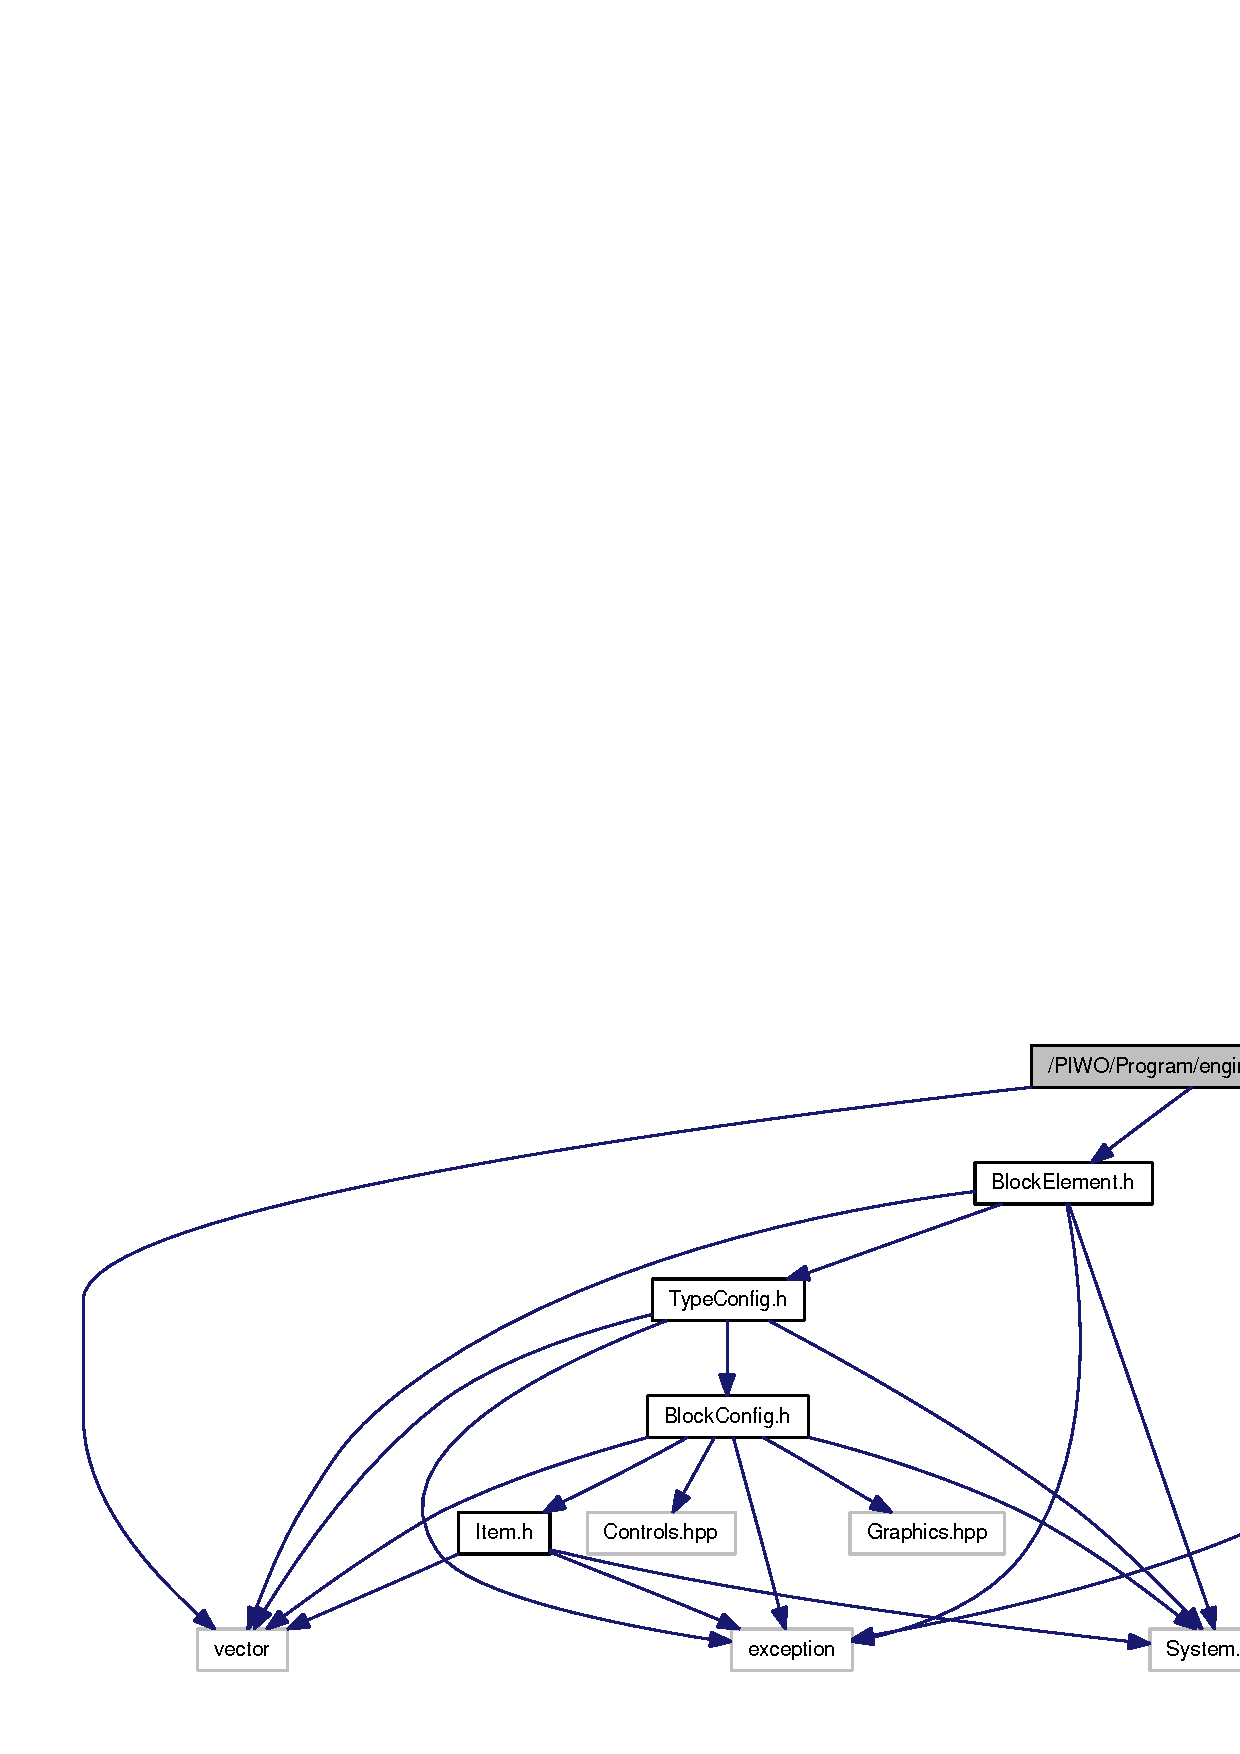
\includegraphics[width=352pt]{BlockOutput_8h__incl}
\end{center}
\end{figure}


This graph shows which files directly or indirectly include this file:\nopagebreak
\begin{figure}[H]
\begin{center}
\leavevmode
\includegraphics[width=420pt]{BlockOutput_8h__dep__incl}
\end{center}
\end{figure}
\subsection*{Classes}
\begin{CompactItemize}
\item 
class \hyperlink{classBlockOutput}{BlockOutput}
\end{CompactItemize}

\hypertarget{Item_8cpp}{
\section{/PIWO/Program/engine/Item.cpp File Reference}
\label{Item_8cpp}\index{/PIWO/Program/engine/Item.cpp@{/PIWO/Program/engine/Item.cpp}}
}
{\tt \#include \char`\"{}Item.h\char`\"{}}\par


Include dependency graph for Item.cpp:\nopagebreak
\begin{figure}[H]
\begin{center}
\leavevmode
\includegraphics[width=124pt]{Item_8cpp__incl}
\end{center}
\end{figure}

\hypertarget{Item_8h}{
\section{/PIWO/Program/engine/Item.h File Reference}
\label{Item_8h}\index{/PIWO/Program/engine/Item.h@{/PIWO/Program/engine/Item.h}}
}
{\tt \#include $<$vector$>$}\par
{\tt \#include $<$System.hpp$>$}\par
{\tt \#include $<$exception$>$}\par


Include dependency graph for Item.h:\nopagebreak
\begin{figure}[H]
\begin{center}
\leavevmode
\includegraphics[width=124pt]{Item_8h__incl}
\end{center}
\end{figure}


This graph shows which files directly or indirectly include this file:\nopagebreak
\begin{figure}[H]
\begin{center}
\leavevmode
\includegraphics[width=420pt]{Item_8h__dep__incl}
\end{center}
\end{figure}
\subsection*{Classes}
\begin{CompactItemize}
\item 
class \hyperlink{classItem}{Item}
\end{CompactItemize}

\hypertarget{TypeConfig_8cpp}{
\section{/PIWO/Program/engine/TypeConfig.cpp File Reference}
\label{TypeConfig_8cpp}\index{/PIWO/Program/engine/TypeConfig.cpp@{/PIWO/Program/engine/TypeConfig.cpp}}
}
{\tt \#include $<$string$>$}\par
{\tt \#include $<$vector$>$}\par
{\tt \#include $<$exception$>$}\par
{\tt \#include \char`\"{}TypeConfig.h\char`\"{}}\par


Include dependency graph for TypeConfig.cpp:\nopagebreak
\begin{figure}[H]
\begin{center}
\leavevmode
\includegraphics[width=296pt]{TypeConfig_8cpp__incl}
\end{center}
\end{figure}

\hypertarget{TypeConfig_8h}{
\section{/PIWO/Program/engine/TypeConfig.h File Reference}
\label{TypeConfig_8h}\index{/PIWO/Program/engine/TypeConfig.h@{/PIWO/Program/engine/TypeConfig.h}}
}
{\tt \#include $<$System.hpp$>$}\par
{\tt \#include $<$vector$>$}\par
{\tt \#include $<$exception$>$}\par
{\tt \#include \char`\"{}BlockConfig.h\char`\"{}}\par


Include dependency graph for TypeConfig.h:\nopagebreak
\begin{figure}[H]
\begin{center}
\leavevmode
\includegraphics[width=233pt]{TypeConfig_8h__incl}
\end{center}
\end{figure}


This graph shows which files directly or indirectly include this file:\nopagebreak
\begin{figure}[H]
\begin{center}
\leavevmode
\includegraphics[width=420pt]{TypeConfig_8h__dep__incl}
\end{center}
\end{figure}
\subsection*{Classes}
\begin{CompactItemize}
\item 
class \hyperlink{classTypeConfig}{TypeConfig}
\end{CompactItemize}

\hypertarget{BlockHistory_8cpp}{
\section{/PIWO/Program/gui/BlockHistory.cpp File Reference}
\label{BlockHistory_8cpp}\index{/PIWO/Program/gui/BlockHistory.cpp@{/PIWO/Program/gui/BlockHistory.cpp}}
}
{\tt \#include $<$vcl.h$>$}\par
{\tt \#include \char`\"{}BlockHistory.h\char`\"{}}\par


Include dependency graph for BlockHistory.cpp:\nopagebreak
\begin{figure}[H]
\begin{center}
\leavevmode
\includegraphics[width=420pt]{BlockHistory_8cpp__incl}
\end{center}
\end{figure}

\hypertarget{BlockHistory_8h}{
\section{/PIWO/Program/gui/BlockHistory.h File Reference}
\label{BlockHistory_8h}\index{/PIWO/Program/gui/BlockHistory.h@{/PIWO/Program/gui/BlockHistory.h}}
}
{\tt \#include \char`\"{}BlockHistoryOutputElement.h\char`\"{}}\par
{\tt \#include \char`\"{}BlockHistoryInputElement.h\char`\"{}}\par
{\tt \#include $<$vector$>$}\par


Include dependency graph for BlockHistory.h:\nopagebreak
\begin{figure}[H]
\begin{center}
\leavevmode
\includegraphics[width=420pt]{BlockHistory_8h__incl}
\end{center}
\end{figure}


This graph shows which files directly or indirectly include this file:\nopagebreak
\begin{figure}[H]
\begin{center}
\leavevmode
\includegraphics[width=420pt]{BlockHistory_8h__dep__incl}
\end{center}
\end{figure}
\subsection*{Classes}
\begin{CompactItemize}
\item 
class \hyperlink{classBlockHistory}{BlockHistory}
\end{CompactItemize}
\subsection*{Typedefs}
\begin{CompactItemize}
\item 
typedef vector$<$ \hyperlink{classBlockHistory}{BlockHistory} $\ast$ $>$ \hyperlink{BlockHistory_8h_1e80e0966c4a2e68a83338258a89f5ae}{vectorBlockHistory}
\end{CompactItemize}


\subsection{Typedef Documentation}
\hypertarget{BlockHistory_8h_1e80e0966c4a2e68a83338258a89f5ae}{
\index{BlockHistory.h@{BlockHistory.h}!vectorBlockHistory@{vectorBlockHistory}}
\index{vectorBlockHistory@{vectorBlockHistory}!BlockHistory.h@{BlockHistory.h}}
\subsubsection[vectorBlockHistory]{\setlength{\rightskip}{0pt plus 5cm}typedef vector$<${\bf BlockHistory}$\ast$$>$ {\bf vectorBlockHistory}}}
\label{BlockHistory_8h_1e80e0966c4a2e68a83338258a89f5ae}




Definition at line 52 of file BlockHistory.h.
\hypertarget{BlockHistoryInputElement_8cpp}{
\section{/PIWO/Program/gui/BlockHistoryInputElement.cpp File Reference}
\label{BlockHistoryInputElement_8cpp}\index{/PIWO/Program/gui/BlockHistoryInputElement.cpp@{/PIWO/Program/gui/BlockHistoryInputElement.cpp}}
}
{\tt \#include $<$vcl.h$>$}\par
{\tt \#include \char`\"{}BlockHistoryInputElement.h\char`\"{}}\par


Include dependency graph for BlockHistoryInputElement.cpp:\nopagebreak
\begin{figure}[H]
\begin{center}
\leavevmode
\includegraphics[width=352pt]{BlockHistoryInputElement_8cpp__incl}
\end{center}
\end{figure}

\hypertarget{BlockHistoryInputElement_8h}{
\section{/PIWO/Program/gui/BlockHistoryInputElement.h File Reference}
\label{BlockHistoryInputElement_8h}\index{/PIWO/Program/gui/BlockHistoryInputElement.h@{/PIWO/Program/gui/BlockHistoryInputElement.h}}
}
{\tt \#include \char`\"{}../engine/BlockInput.h\char`\"{}}\par
{\tt \#include \char`\"{}../engine/TypeConfig.h\char`\"{}}\par


Include dependency graph for BlockHistoryInputElement.h:\nopagebreak
\begin{figure}[H]
\begin{center}
\leavevmode
\includegraphics[width=352pt]{BlockHistoryInputElement_8h__incl}
\end{center}
\end{figure}


This graph shows which files directly or indirectly include this file:\nopagebreak
\begin{figure}[H]
\begin{center}
\leavevmode
\includegraphics[width=420pt]{BlockHistoryInputElement_8h__dep__incl}
\end{center}
\end{figure}
\subsection*{Classes}
\begin{CompactItemize}
\item 
class \hyperlink{classBlockHistoryInputElement}{BlockHistoryInputElement}
\end{CompactItemize}

\hypertarget{BlockHistoryOutputElement_8cpp}{
\section{/PIWO/Program/gui/BlockHistoryOutputElement.cpp File Reference}
\label{BlockHistoryOutputElement_8cpp}\index{/PIWO/Program/gui/BlockHistoryOutputElement.cpp@{/PIWO/Program/gui/BlockHistoryOutputElement.cpp}}
}
{\tt \#include $<$vcl.h$>$}\par
{\tt \#include \char`\"{}BlockHistoryOutputElement.h\char`\"{}}\par


Include dependency graph for BlockHistoryOutputElement.cpp:\nopagebreak
\begin{figure}[H]
\begin{center}
\leavevmode
\includegraphics[width=352pt]{BlockHistoryOutputElement_8cpp__incl}
\end{center}
\end{figure}

\hypertarget{BlockHistoryOutputElement_8h}{
\section{/PIWO/Program/gui/BlockHistoryOutputElement.h File Reference}
\label{BlockHistoryOutputElement_8h}\index{/PIWO/Program/gui/BlockHistoryOutputElement.h@{/PIWO/Program/gui/BlockHistoryOutputElement.h}}
}
{\tt \#include \char`\"{}../engine/BlockOutput.h\char`\"{}}\par
{\tt \#include \char`\"{}../engine/TypeConfig.h\char`\"{}}\par


Include dependency graph for BlockHistoryOutputElement.h:\nopagebreak
\begin{figure}[H]
\begin{center}
\leavevmode
\includegraphics[width=352pt]{BlockHistoryOutputElement_8h__incl}
\end{center}
\end{figure}


This graph shows which files directly or indirectly include this file:\nopagebreak
\begin{figure}[H]
\begin{center}
\leavevmode
\includegraphics[width=420pt]{BlockHistoryOutputElement_8h__dep__incl}
\end{center}
\end{figure}
\subsection*{Classes}
\begin{CompactItemize}
\item 
class \hyperlink{classBlockHistoryOutputElement}{BlockHistoryOutputElement}
\end{CompactItemize}

\hypertarget{BlockValidateInputElement_8h}{
\section{/PIWO/Program/gui/BlockValidateInputElement.h File Reference}
\label{BlockValidateInputElement_8h}\index{/PIWO/Program/gui/BlockValidateInputElement.h@{/PIWO/Program/gui/BlockValidateInputElement.h}}
}
{\tt \#include \char`\"{}../engine/BlockInput.h\char`\"{}}\par
{\tt \#include \char`\"{}Connection.h\char`\"{}}\par


Include dependency graph for BlockValidateInputElement.h:\nopagebreak
\begin{figure}[H]
\begin{center}
\leavevmode
\includegraphics[width=420pt]{BlockValidateInputElement_8h__incl}
\end{center}
\end{figure}


This graph shows which files directly or indirectly include this file:\nopagebreak
\begin{figure}[H]
\begin{center}
\leavevmode
\includegraphics[width=136pt]{BlockValidateInputElement_8h__dep__incl}
\end{center}
\end{figure}
\subsection*{Classes}
\begin{CompactItemize}
\item 
class \hyperlink{classBlockValidateInputElement}{BlockValidateInputElement}
\end{CompactItemize}

\hypertarget{BlockValidateOutputElement_8h}{
\section{/PIWO/Program/gui/BlockValidateOutputElement.h File Reference}
\label{BlockValidateOutputElement_8h}\index{/PIWO/Program/gui/BlockValidateOutputElement.h@{/PIWO/Program/gui/BlockValidateOutputElement.h}}
}
{\tt \#include \char`\"{}../engine/BlockOutput.h\char`\"{}}\par
{\tt \#include \char`\"{}Connection.h\char`\"{}}\par
{\tt \#include $<$vector$>$}\par


Include dependency graph for BlockValidateOutputElement.h:\nopagebreak
\begin{figure}[H]
\begin{center}
\leavevmode
\includegraphics[width=420pt]{BlockValidateOutputElement_8h__incl}
\end{center}
\end{figure}


This graph shows which files directly or indirectly include this file:\nopagebreak
\begin{figure}[H]
\begin{center}
\leavevmode
\includegraphics[width=140pt]{BlockValidateOutputElement_8h__dep__incl}
\end{center}
\end{figure}
\subsection*{Classes}
\begin{CompactItemize}
\item 
class \hyperlink{classBlockValidateOutputElement}{BlockValidateOutputElement}
\end{CompactItemize}

\hypertarget{Connection_8cpp}{
\section{/PIWO/Program/gui/Connection.cpp File Reference}
\label{Connection_8cpp}\index{/PIWO/Program/gui/Connection.cpp@{/PIWO/Program/gui/Connection.cpp}}
}
{\tt \#include $<$vcl.h$>$}\par
{\tt \#include \char`\"{}Connection.h\char`\"{}}\par


Include dependency graph for Connection.cpp:\nopagebreak
\begin{figure}[H]
\begin{center}
\leavevmode
\includegraphics[width=420pt]{Connection_8cpp__incl}
\end{center}
\end{figure}

\hypertarget{Connection_8h}{
\section{/PIWO/Program/gui/Connection.h File Reference}
\label{Connection_8h}\index{/PIWO/Program/gui/Connection.h@{/PIWO/Program/gui/Connection.h}}
}
{\tt \#include $<$SysUtils.hpp$>$}\par
{\tt \#include $<$Classes.hpp$>$}\par
{\tt \#include $<$Controls.hpp$>$}\par
{\tt \#include $<$vector$>$}\par
{\tt \#include \char`\"{}../engine/BlockInput.h\char`\"{}}\par
{\tt \#include \char`\"{}../engine/BlockOutput.h\char`\"{}}\par
{\tt \#include \char`\"{}Line.h\char`\"{}}\par
{\tt \#include \char`\"{}VisualBlock.h\char`\"{}}\par


Include dependency graph for Connection.h:\nopagebreak
\begin{figure}[H]
\begin{center}
\leavevmode
\includegraphics[width=420pt]{Connection_8h__incl}
\end{center}
\end{figure}


This graph shows which files directly or indirectly include this file:\nopagebreak
\begin{figure}[H]
\begin{center}
\leavevmode
\includegraphics[width=420pt]{Connection_8h__dep__incl}
\end{center}
\end{figure}
\subsection*{Classes}
\begin{CompactItemize}
\item 
class \hyperlink{classConnection}{Connection}
\end{CompactItemize}
\subsection*{Defines}
\begin{CompactItemize}
\item 
\#define \hyperlink{Connection_8h_b00477876fb393bb501e5cdf2c3dd390}{CONNECTION\_\-OK\_\-NORMAL}~0x33CC33
\item 
\#define \hyperlink{Connection_8h_f9125b98ea55fc4aea8ef73df27f1a13}{CONNECTION\_\-OK\_\-SELECTED}~0x20FF20
\item 
\#define \hyperlink{Connection_8h_529b378e03bb2eb7190f7c19c1a86467}{CONNECTION\_\-WARRNING\_\-NORMAL}~61137
\item 
\#define \hyperlink{Connection_8h_4533220d4269a55b041d2a98924984e9}{CONNECTION\_\-WARRNING\_\-SELECTED}~65021
\item 
\#define \hyperlink{Connection_8h_2233f4351cd7d445f7b5cc129a3aa33d}{CONNECTION\_\-ERROR\_\-NORMAL}~206
\item 
\#define \hyperlink{Connection_8h_49b81d66da221f9930a7e56f13eb45ce}{CONNECTION\_\-ERROR\_\-SELECTED}~255
\end{CompactItemize}
\subsection*{Typedefs}
\begin{CompactItemize}
\item 
typedef void(\_\-\_\-closure $\ast$ \hyperlink{Connection_8h_e18f1161e76df22142d73ed0734bd10c}{Connection\_\-Function} )(void $\ast$)
\end{CompactItemize}
\subsection*{Variables}
\begin{CompactItemize}
\item 
static const TColor \hyperlink{Connection_8h_6ed6ea9c3159ba44124dbac86618f618}{ConnectionOkNormalColor} = CONNECTION\_\-OK\_\-NORMAL
\item 
static const TColor \hyperlink{Connection_8h_d4c99c958d868dcd86be916461609e24}{ConnectionOkSelectedColor} = CONNECTION\_\-OK\_\-SELECTED
\item 
static const TColor \hyperlink{Connection_8h_8a3f1370822008c6a871b862f01bccbf}{ConnectionWarrningNormalColor} = CONNECTION\_\-WARRNING\_\-NORMAL
\item 
static const TColor \hyperlink{Connection_8h_8a82b0bcaeea557de65e39bf2399c308}{ConnectionWarrningSelectedColor} = CONNECTION\_\-WARRNING\_\-SELECTED
\item 
static const TColor \hyperlink{Connection_8h_010346520e0d6678335b6b59f77bc690}{ConnectionErrorNormalColor} = CONNECTION\_\-ERROR\_\-NORMAL
\item 
static const TColor \hyperlink{Connection_8h_dc0b2e1af561f6aa5d3396accfd6ed91}{ConnectionErrorSelectedColor} = CONNECTION\_\-ERROR\_\-SELECTED
\end{CompactItemize}


\subsection{Define Documentation}
\hypertarget{Connection_8h_2233f4351cd7d445f7b5cc129a3aa33d}{
\index{Connection.h@{Connection.h}!CONNECTION\_\-ERROR\_\-NORMAL@{CONNECTION\_\-ERROR\_\-NORMAL}}
\index{CONNECTION\_\-ERROR\_\-NORMAL@{CONNECTION\_\-ERROR\_\-NORMAL}!Connection.h@{Connection.h}}
\subsubsection[CONNECTION\_\-ERROR\_\-NORMAL]{\setlength{\rightskip}{0pt plus 5cm}\#define CONNECTION\_\-ERROR\_\-NORMAL~206}}
\label{Connection_8h_2233f4351cd7d445f7b5cc129a3aa33d}




Definition at line 16 of file Connection.h.\hypertarget{Connection_8h_49b81d66da221f9930a7e56f13eb45ce}{
\index{Connection.h@{Connection.h}!CONNECTION\_\-ERROR\_\-SELECTED@{CONNECTION\_\-ERROR\_\-SELECTED}}
\index{CONNECTION\_\-ERROR\_\-SELECTED@{CONNECTION\_\-ERROR\_\-SELECTED}!Connection.h@{Connection.h}}
\subsubsection[CONNECTION\_\-ERROR\_\-SELECTED]{\setlength{\rightskip}{0pt plus 5cm}\#define CONNECTION\_\-ERROR\_\-SELECTED~255}}
\label{Connection_8h_49b81d66da221f9930a7e56f13eb45ce}




Definition at line 17 of file Connection.h.\hypertarget{Connection_8h_b00477876fb393bb501e5cdf2c3dd390}{
\index{Connection.h@{Connection.h}!CONNECTION\_\-OK\_\-NORMAL@{CONNECTION\_\-OK\_\-NORMAL}}
\index{CONNECTION\_\-OK\_\-NORMAL@{CONNECTION\_\-OK\_\-NORMAL}!Connection.h@{Connection.h}}
\subsubsection[CONNECTION\_\-OK\_\-NORMAL]{\setlength{\rightskip}{0pt plus 5cm}\#define CONNECTION\_\-OK\_\-NORMAL~0x33CC33}}
\label{Connection_8h_b00477876fb393bb501e5cdf2c3dd390}




Definition at line 12 of file Connection.h.\hypertarget{Connection_8h_f9125b98ea55fc4aea8ef73df27f1a13}{
\index{Connection.h@{Connection.h}!CONNECTION\_\-OK\_\-SELECTED@{CONNECTION\_\-OK\_\-SELECTED}}
\index{CONNECTION\_\-OK\_\-SELECTED@{CONNECTION\_\-OK\_\-SELECTED}!Connection.h@{Connection.h}}
\subsubsection[CONNECTION\_\-OK\_\-SELECTED]{\setlength{\rightskip}{0pt plus 5cm}\#define CONNECTION\_\-OK\_\-SELECTED~0x20FF20}}
\label{Connection_8h_f9125b98ea55fc4aea8ef73df27f1a13}




Definition at line 13 of file Connection.h.\hypertarget{Connection_8h_529b378e03bb2eb7190f7c19c1a86467}{
\index{Connection.h@{Connection.h}!CONNECTION\_\-WARRNING\_\-NORMAL@{CONNECTION\_\-WARRNING\_\-NORMAL}}
\index{CONNECTION\_\-WARRNING\_\-NORMAL@{CONNECTION\_\-WARRNING\_\-NORMAL}!Connection.h@{Connection.h}}
\subsubsection[CONNECTION\_\-WARRNING\_\-NORMAL]{\setlength{\rightskip}{0pt plus 5cm}\#define CONNECTION\_\-WARRNING\_\-NORMAL~61137}}
\label{Connection_8h_529b378e03bb2eb7190f7c19c1a86467}




Definition at line 14 of file Connection.h.\hypertarget{Connection_8h_4533220d4269a55b041d2a98924984e9}{
\index{Connection.h@{Connection.h}!CONNECTION\_\-WARRNING\_\-SELECTED@{CONNECTION\_\-WARRNING\_\-SELECTED}}
\index{CONNECTION\_\-WARRNING\_\-SELECTED@{CONNECTION\_\-WARRNING\_\-SELECTED}!Connection.h@{Connection.h}}
\subsubsection[CONNECTION\_\-WARRNING\_\-SELECTED]{\setlength{\rightskip}{0pt plus 5cm}\#define CONNECTION\_\-WARRNING\_\-SELECTED~65021}}
\label{Connection_8h_4533220d4269a55b041d2a98924984e9}




Definition at line 15 of file Connection.h.

\subsection{Typedef Documentation}
\hypertarget{Connection_8h_e18f1161e76df22142d73ed0734bd10c}{
\index{Connection.h@{Connection.h}!Connection\_\-Function@{Connection\_\-Function}}
\index{Connection\_\-Function@{Connection\_\-Function}!Connection.h@{Connection.h}}
\subsubsection[Connection\_\-Function]{\setlength{\rightskip}{0pt plus 5cm}typedef void(\_\-\_\-closure $\ast$ {\bf Connection\_\-Function})(void $\ast$)}}
\label{Connection_8h_e18f1161e76df22142d73ed0734bd10c}




Definition at line 26 of file Connection.h.

\subsection{Variable Documentation}
\hypertarget{Connection_8h_010346520e0d6678335b6b59f77bc690}{
\index{Connection.h@{Connection.h}!ConnectionErrorNormalColor@{ConnectionErrorNormalColor}}
\index{ConnectionErrorNormalColor@{ConnectionErrorNormalColor}!Connection.h@{Connection.h}}
\subsubsection[ConnectionErrorNormalColor]{\setlength{\rightskip}{0pt plus 5cm}const TColor {\bf ConnectionErrorNormalColor} = CONNECTION\_\-ERROR\_\-NORMAL\hspace{0.3cm}{\tt  \mbox{[}static\mbox{]}}}}
\label{Connection_8h_010346520e0d6678335b6b59f77bc690}




Definition at line 23 of file Connection.h.

Referenced by Connection::setSelected(), and Connection::update().\hypertarget{Connection_8h_dc0b2e1af561f6aa5d3396accfd6ed91}{
\index{Connection.h@{Connection.h}!ConnectionErrorSelectedColor@{ConnectionErrorSelectedColor}}
\index{ConnectionErrorSelectedColor@{ConnectionErrorSelectedColor}!Connection.h@{Connection.h}}
\subsubsection[ConnectionErrorSelectedColor]{\setlength{\rightskip}{0pt plus 5cm}const TColor {\bf ConnectionErrorSelectedColor} = CONNECTION\_\-ERROR\_\-SELECTED\hspace{0.3cm}{\tt  \mbox{[}static\mbox{]}}}}
\label{Connection_8h_dc0b2e1af561f6aa5d3396accfd6ed91}




Definition at line 24 of file Connection.h.

Referenced by Connection::setSelected(), and Connection::update().\hypertarget{Connection_8h_6ed6ea9c3159ba44124dbac86618f618}{
\index{Connection.h@{Connection.h}!ConnectionOkNormalColor@{ConnectionOkNormalColor}}
\index{ConnectionOkNormalColor@{ConnectionOkNormalColor}!Connection.h@{Connection.h}}
\subsubsection[ConnectionOkNormalColor]{\setlength{\rightskip}{0pt plus 5cm}const TColor {\bf ConnectionOkNormalColor} = CONNECTION\_\-OK\_\-NORMAL\hspace{0.3cm}{\tt  \mbox{[}static\mbox{]}}}}
\label{Connection_8h_6ed6ea9c3159ba44124dbac86618f618}




Definition at line 19 of file Connection.h.

Referenced by Connection::setSelected(), and Connection::update().\hypertarget{Connection_8h_d4c99c958d868dcd86be916461609e24}{
\index{Connection.h@{Connection.h}!ConnectionOkSelectedColor@{ConnectionOkSelectedColor}}
\index{ConnectionOkSelectedColor@{ConnectionOkSelectedColor}!Connection.h@{Connection.h}}
\subsubsection[ConnectionOkSelectedColor]{\setlength{\rightskip}{0pt plus 5cm}const TColor {\bf ConnectionOkSelectedColor} = CONNECTION\_\-OK\_\-SELECTED\hspace{0.3cm}{\tt  \mbox{[}static\mbox{]}}}}
\label{Connection_8h_d4c99c958d868dcd86be916461609e24}




Definition at line 20 of file Connection.h.

Referenced by Connection::setSelected(), and Connection::update().\hypertarget{Connection_8h_8a3f1370822008c6a871b862f01bccbf}{
\index{Connection.h@{Connection.h}!ConnectionWarrningNormalColor@{ConnectionWarrningNormalColor}}
\index{ConnectionWarrningNormalColor@{ConnectionWarrningNormalColor}!Connection.h@{Connection.h}}
\subsubsection[ConnectionWarrningNormalColor]{\setlength{\rightskip}{0pt plus 5cm}const TColor {\bf ConnectionWarrningNormalColor} = CONNECTION\_\-WARRNING\_\-NORMAL\hspace{0.3cm}{\tt  \mbox{[}static\mbox{]}}}}
\label{Connection_8h_8a3f1370822008c6a871b862f01bccbf}




Definition at line 21 of file Connection.h.

Referenced by Connection::setSelected(), and Connection::update().\hypertarget{Connection_8h_8a82b0bcaeea557de65e39bf2399c308}{
\index{Connection.h@{Connection.h}!ConnectionWarrningSelectedColor@{ConnectionWarrningSelectedColor}}
\index{ConnectionWarrningSelectedColor@{ConnectionWarrningSelectedColor}!Connection.h@{Connection.h}}
\subsubsection[ConnectionWarrningSelectedColor]{\setlength{\rightskip}{0pt plus 5cm}const TColor {\bf ConnectionWarrningSelectedColor} = CONNECTION\_\-WARRNING\_\-SELECTED\hspace{0.3cm}{\tt  \mbox{[}static\mbox{]}}}}
\label{Connection_8h_8a82b0bcaeea557de65e39bf2399c308}




Definition at line 22 of file Connection.h.

Referenced by Connection::setSelected(), and Connection::update().
\hypertarget{history_8cpp}{
\section{/PIWO/Program/gui/history.cpp File Reference}
\label{history_8cpp}\index{/PIWO/Program/gui/history.cpp@{/PIWO/Program/gui/history.cpp}}
}
{\tt \#include $<$vcl.h$>$}\par
{\tt \#include \char`\"{}history.h\char`\"{}}\par


Include dependency graph for history.cpp:\nopagebreak
\begin{figure}[H]
\begin{center}
\leavevmode
\includegraphics[width=420pt]{history_8cpp__incl}
\end{center}
\end{figure}

\hypertarget{history_8h}{
\section{/PIWO/Program/gui/history.h File Reference}
\label{history_8h}\index{/PIWO/Program/gui/history.h@{/PIWO/Program/gui/history.h}}
}
{\tt \#include $<$Classes.hpp$>$}\par
{\tt \#include $<$Controls.hpp$>$}\par
{\tt \#include $<$StdCtrls.hpp$>$}\par
{\tt \#include $<$Forms.hpp$>$}\par
{\tt \#include $<$ActnList.hpp$>$}\par
{\tt \#include $<$ComCtrls.hpp$>$}\par
{\tt \#include $<$StdActns.hpp$>$}\par
{\tt \#include $<$ToolWin.hpp$>$}\par
{\tt \#include \char`\"{}VisualBlock.h\char`\"{}}\par
{\tt \#include \char`\"{}../brige/PluginContener.h\char`\"{}}\par
{\tt \#include $<$ImgList.hpp$>$}\par
{\tt \#include $<$Buttons.hpp$>$}\par
{\tt \#include $<$ExtCtrls.hpp$>$}\par
{\tt \#include $<$vector$>$}\par


Include dependency graph for history.h:\nopagebreak
\begin{figure}[H]
\begin{center}
\leavevmode
\includegraphics[width=420pt]{history_8h__incl}
\end{center}
\end{figure}


This graph shows which files directly or indirectly include this file:\nopagebreak
\begin{figure}[H]
\begin{center}
\leavevmode
\includegraphics[width=221pt]{history_8h__dep__incl}
\end{center}
\end{figure}
\subsection*{Classes}
\begin{CompactItemize}
\item 
class \hyperlink{classTHistory}{THistory}
\end{CompactItemize}

\hypertarget{Line_8cpp}{
\section{/PIWO/Program/gui/Line.cpp File Reference}
\label{Line_8cpp}\index{/PIWO/Program/gui/Line.cpp@{/PIWO/Program/gui/Line.cpp}}
}
{\tt \#include $<$vcl.h$>$}\par
{\tt \#include \char`\"{}Line.h\char`\"{}}\par


Include dependency graph for Line.cpp:\nopagebreak
\begin{figure}[H]
\begin{center}
\leavevmode
\includegraphics[width=146pt]{Line_8cpp__incl}
\end{center}
\end{figure}

\hypertarget{Line_8h}{
\section{/PIWO/Program/gui/Line.h File Reference}
\label{Line_8h}\index{/PIWO/Program/gui/Line.h@{/PIWO/Program/gui/Line.h}}
}
{\tt \#include $<$SysUtils.hpp$>$}\par
{\tt \#include $<$Classes.hpp$>$}\par
{\tt \#include $<$Controls.hpp$>$}\par


Include dependency graph for Line.h:\nopagebreak
\begin{figure}[H]
\begin{center}
\leavevmode
\includegraphics[width=146pt]{Line_8h__incl}
\end{center}
\end{figure}


This graph shows which files directly or indirectly include this file:\nopagebreak
\begin{figure}[H]
\begin{center}
\leavevmode
\includegraphics[width=420pt]{Line_8h__dep__incl}
\end{center}
\end{figure}
\subsection*{Classes}
\begin{CompactItemize}
\item 
class \hyperlink{classLine}{Line}
\end{CompactItemize}
\subsection*{Typedefs}
\begin{CompactItemize}
\item 
typedef void(\_\-\_\-closure $\ast$ \hyperlink{Line_8h_9dd4ddd90e5216119027c0f379889e85}{Line\_\-Function} )(TObject $\ast$)
\end{CompactItemize}


\subsection{Typedef Documentation}
\hypertarget{Line_8h_9dd4ddd90e5216119027c0f379889e85}{
\index{Line.h@{Line.h}!Line\_\-Function@{Line\_\-Function}}
\index{Line\_\-Function@{Line\_\-Function}!Line.h@{Line.h}}
\subsubsection[Line\_\-Function]{\setlength{\rightskip}{0pt plus 5cm}typedef void(\_\-\_\-closure $\ast$ {\bf Line\_\-Function})(TObject $\ast$)}}
\label{Line_8h_9dd4ddd90e5216119027c0f379889e85}




Definition at line 7 of file Line.h.
\hypertarget{PIWOEngine_8cpp}{
\section{/PIWO/Program/gui/PIWOEngine.cpp File Reference}
\label{PIWOEngine_8cpp}\index{/PIWO/Program/gui/PIWOEngine.cpp@{/PIWO/Program/gui/PIWOEngine.cpp}}
}
{\tt \#include $<$vcl.h$>$}\par
{\tt \#include \char`\"{}PIWOEngine.h\char`\"{}}\par
{\tt \#include \char`\"{}BlockValidateInputElement.h\char`\"{}}\par
{\tt \#include \char`\"{}BlockValidateOutputElement.h\char`\"{}}\par


Include dependency graph for PIWOEngine.cpp:\nopagebreak
\begin{figure}[H]
\begin{center}
\leavevmode
\includegraphics[width=420pt]{PIWOEngine_8cpp__incl}
\end{center}
\end{figure}
\subsection*{Functions}
\begin{CompactItemize}
\item 
void \hyperlink{PIWOEngine_8cpp_7c7d32818ebae2fe8c04f6a654168292}{putString} (const AnsiString \&str, TStream \&stream)
\item 
void \hyperlink{PIWOEngine_8cpp_b52bb01401fbc44c520cbc48a7949b36}{putInt} (const int i, TStream \&stream)
\item 
AnsiString \hyperlink{PIWOEngine_8cpp_de6df329afe49e49a29cc8242f1c2473}{getString} (TStream \&stream)
\item 
int \hyperlink{PIWOEngine_8cpp_5f408adb07e4c71f31021eebf607161d}{getInt} (TStream \&stream)
\end{CompactItemize}


\subsection{Function Documentation}
\hypertarget{PIWOEngine_8cpp_5f408adb07e4c71f31021eebf607161d}{
\index{PIWOEngine.cpp@{PIWOEngine.cpp}!getInt@{getInt}}
\index{getInt@{getInt}!PIWOEngine.cpp@{PIWOEngine.cpp}}
\subsubsection[getInt]{\setlength{\rightskip}{0pt plus 5cm}int getInt (TStream \& {\em stream})}}
\label{PIWOEngine_8cpp_5f408adb07e4c71f31021eebf607161d}


Pobiera integer z stream \begin{Desc}
\item[Parameters:]
\begin{description}
\item[{\em stream}]stream \end{description}
\end{Desc}
\begin{Desc}
\item[Returns:]integer \end{Desc}


Definition at line 2528 of file PIWOEngine.cpp.

Referenced by PIWOEngine::loadFromFile().\hypertarget{PIWOEngine_8cpp_de6df329afe49e49a29cc8242f1c2473}{
\index{PIWOEngine.cpp@{PIWOEngine.cpp}!getString@{getString}}
\index{getString@{getString}!PIWOEngine.cpp@{PIWOEngine.cpp}}
\subsubsection[getString]{\setlength{\rightskip}{0pt plus 5cm}AnsiString getString (TStream \& {\em stream})}}
\label{PIWOEngine_8cpp_de6df329afe49e49a29cc8242f1c2473}


Pobiera string z stream \begin{Desc}
\item[Parameters:]
\begin{description}
\item[{\em stream}]stream \end{description}
\end{Desc}
\begin{Desc}
\item[Returns:]string \end{Desc}


Definition at line 2515 of file PIWOEngine.cpp.

Referenced by PIWOEngine::loadFromFile().\hypertarget{PIWOEngine_8cpp_b52bb01401fbc44c520cbc48a7949b36}{
\index{PIWOEngine.cpp@{PIWOEngine.cpp}!putInt@{putInt}}
\index{putInt@{putInt}!PIWOEngine.cpp@{PIWOEngine.cpp}}
\subsubsection[putInt]{\setlength{\rightskip}{0pt plus 5cm}void putInt (const int {\em i}, \/  TStream \& {\em stream})}}
\label{PIWOEngine_8cpp_b52bb01401fbc44c520cbc48a7949b36}


Zapisuje integer do stream \begin{Desc}
\item[Parameters:]
\begin{description}
\item[{\em i}]integer \item[{\em stream}]stream \end{description}
\end{Desc}


Definition at line 2510 of file PIWOEngine.cpp.

Referenced by PIWOEngine::saveToFile().\hypertarget{PIWOEngine_8cpp_7c7d32818ebae2fe8c04f6a654168292}{
\index{PIWOEngine.cpp@{PIWOEngine.cpp}!putString@{putString}}
\index{putString@{putString}!PIWOEngine.cpp@{PIWOEngine.cpp}}
\subsubsection[putString]{\setlength{\rightskip}{0pt plus 5cm}void putString (const AnsiString \& {\em str}, \/  TStream \& {\em stream})}}
\label{PIWOEngine_8cpp_7c7d32818ebae2fe8c04f6a654168292}


Zapisuje string do stream \begin{Desc}
\item[Parameters:]
\begin{description}
\item[{\em str}]string \item[{\em stream}]stream \end{description}
\end{Desc}


Definition at line 2502 of file PIWOEngine.cpp.

Referenced by PIWOEngine::saveToFile().
\hypertarget{PIWOEngine_8h}{
\section{/PIWO/Program/gui/PIWOEngine.h File Reference}
\label{PIWOEngine_8h}\index{/PIWO/Program/gui/PIWOEngine.h@{/PIWO/Program/gui/PIWOEngine.h}}
}
{\tt \#include $<$SysUtils.hpp$>$}\par
{\tt \#include $<$Classes.hpp$>$}\par
{\tt \#include $<$Controls.hpp$>$}\par
{\tt \#include $<$Forms.hpp$>$}\par
{\tt \#include \char`\"{}../brige/PluginContener.h\char`\"{}}\par
{\tt \#include \char`\"{}VisualBlock.h\char`\"{}}\par
{\tt \#include \char`\"{}Connection.h\char`\"{}}\par
{\tt \#include \char`\"{}history.h\char`\"{}}\par


Include dependency graph for PIWOEngine.h:\nopagebreak
\begin{figure}[H]
\begin{center}
\leavevmode
\includegraphics[width=420pt]{PIWOEngine_8h__incl}
\end{center}
\end{figure}


This graph shows which files directly or indirectly include this file:\nopagebreak
\begin{figure}[H]
\begin{center}
\leavevmode
\includegraphics[width=181pt]{PIWOEngine_8h__dep__incl}
\end{center}
\end{figure}
\subsection*{Classes}
\begin{CompactItemize}
\item 
class \hyperlink{classPIWOEngine}{PIWOEngine}
\end{CompactItemize}
\subsection*{Defines}
\begin{CompactItemize}
\item 
\#define \hyperlink{PIWOEngine_8h_8327c4bf47fc65dfd8590b9566109b44}{PIWOEngineH}
\item 
\#define \hyperlink{PIWOEngine_8h_318dcd0c0a579276e1ad2effdbd5a003}{PIWOMAINCLASSTYPE}~TScrollBox
\end{CompactItemize}
\subsection*{Typedefs}
\begin{CompactItemize}
\item 
typedef const \hyperlink{PIWOEngine_8h_ae0fdfb65731fcd8dad6e5c841767865}{AnsiString}
\item 
typedef void(\_\-\_\-closure $\ast$ \hyperlink{PIWOEngine_8h_8273eb67828fc9cc4e2b18b930dada38}{PIWOEngine\_\-RunProgress} )(TObject $\ast$, const AnsiString, const double)
\end{CompactItemize}
\subsection*{Functions}
\begin{CompactItemize}
\item 
typedef \hyperlink{PIWOEngine_8h_83030218b6b54cb750b32041e06ead2e}{void} (\_\-\_\-closure $\ast$PIWOEngine\_\-Log)(TObject $\ast$
\item 
void \hyperlink{PIWOEngine_8h_7c7d32818ebae2fe8c04f6a654168292}{putString} (const AnsiString \&str, TStream \&stream)
\item 
void \hyperlink{PIWOEngine_8h_b52bb01401fbc44c520cbc48a7949b36}{putInt} (const int i, TStream \&stream)
\item 
AnsiString \hyperlink{PIWOEngine_8h_de6df329afe49e49a29cc8242f1c2473}{getString} (TStream \&stream)
\item 
int \hyperlink{PIWOEngine_8h_5f408adb07e4c71f31021eebf607161d}{getInt} (TStream \&stream)
\end{CompactItemize}


\subsection{Define Documentation}
\hypertarget{PIWOEngine_8h_8327c4bf47fc65dfd8590b9566109b44}{
\index{PIWOEngine.h@{PIWOEngine.h}!PIWOEngineH@{PIWOEngineH}}
\index{PIWOEngineH@{PIWOEngineH}!PIWOEngine.h@{PIWOEngine.h}}
\subsubsection[PIWOEngineH]{\setlength{\rightskip}{0pt plus 5cm}\#define PIWOEngineH}}
\label{PIWOEngine_8h_8327c4bf47fc65dfd8590b9566109b44}




Definition at line 2 of file PIWOEngine.h.\hypertarget{PIWOEngine_8h_318dcd0c0a579276e1ad2effdbd5a003}{
\index{PIWOEngine.h@{PIWOEngine.h}!PIWOMAINCLASSTYPE@{PIWOMAINCLASSTYPE}}
\index{PIWOMAINCLASSTYPE@{PIWOMAINCLASSTYPE}!PIWOEngine.h@{PIWOEngine.h}}
\subsubsection[PIWOMAINCLASSTYPE]{\setlength{\rightskip}{0pt plus 5cm}\#define PIWOMAINCLASSTYPE~TScrollBox}}
\label{PIWOEngine_8h_318dcd0c0a579276e1ad2effdbd5a003}




Definition at line 13 of file PIWOEngine.h.

Referenced by VisualBlock::BlockMouseDown(), VisualBlock::BlockMouseUp(), and PIWOEngine::PIWOEngine().

\subsection{Typedef Documentation}
\hypertarget{PIWOEngine_8h_ae0fdfb65731fcd8dad6e5c841767865}{
\index{PIWOEngine.h@{PIWOEngine.h}!AnsiString@{AnsiString}}
\index{AnsiString@{AnsiString}!PIWOEngine.h@{PIWOEngine.h}}
\subsubsection[AnsiString]{\setlength{\rightskip}{0pt plus 5cm}typedef const AnsiString}}
\label{PIWOEngine_8h_ae0fdfb65731fcd8dad6e5c841767865}




Definition at line 15 of file PIWOEngine.h.\hypertarget{PIWOEngine_8h_8273eb67828fc9cc4e2b18b930dada38}{
\index{PIWOEngine.h@{PIWOEngine.h}!PIWOEngine\_\-RunProgress@{PIWOEngine\_\-RunProgress}}
\index{PIWOEngine\_\-RunProgress@{PIWOEngine\_\-RunProgress}!PIWOEngine.h@{PIWOEngine.h}}
\subsubsection[PIWOEngine\_\-RunProgress]{\setlength{\rightskip}{0pt plus 5cm}typedef void(\_\-\_\-closure $\ast$ {\bf PIWOEngine\_\-RunProgress})(TObject $\ast$, const AnsiString, const double)}}
\label{PIWOEngine_8h_8273eb67828fc9cc4e2b18b930dada38}




Definition at line 16 of file PIWOEngine.h.

\subsection{Function Documentation}
\hypertarget{PIWOEngine_8h_5f408adb07e4c71f31021eebf607161d}{
\index{PIWOEngine.h@{PIWOEngine.h}!getInt@{getInt}}
\index{getInt@{getInt}!PIWOEngine.h@{PIWOEngine.h}}
\subsubsection[getInt]{\setlength{\rightskip}{0pt plus 5cm}int getInt (TStream \& {\em stream})}}
\label{PIWOEngine_8h_5f408adb07e4c71f31021eebf607161d}


Pobiera integer z stream \begin{Desc}
\item[Parameters:]
\begin{description}
\item[{\em stream}]stream \end{description}
\end{Desc}
\begin{Desc}
\item[Returns:]integer \end{Desc}


Definition at line 2528 of file PIWOEngine.cpp.

Referenced by PIWOEngine::loadFromFile().\hypertarget{PIWOEngine_8h_de6df329afe49e49a29cc8242f1c2473}{
\index{PIWOEngine.h@{PIWOEngine.h}!getString@{getString}}
\index{getString@{getString}!PIWOEngine.h@{PIWOEngine.h}}
\subsubsection[getString]{\setlength{\rightskip}{0pt plus 5cm}AnsiString getString (TStream \& {\em stream})}}
\label{PIWOEngine_8h_de6df329afe49e49a29cc8242f1c2473}


Pobiera string z stream \begin{Desc}
\item[Parameters:]
\begin{description}
\item[{\em stream}]stream \end{description}
\end{Desc}
\begin{Desc}
\item[Returns:]string \end{Desc}


Definition at line 2515 of file PIWOEngine.cpp.

Referenced by PIWOEngine::loadFromFile().\hypertarget{PIWOEngine_8h_b52bb01401fbc44c520cbc48a7949b36}{
\index{PIWOEngine.h@{PIWOEngine.h}!putInt@{putInt}}
\index{putInt@{putInt}!PIWOEngine.h@{PIWOEngine.h}}
\subsubsection[putInt]{\setlength{\rightskip}{0pt plus 5cm}void putInt (const int {\em i}, \/  TStream \& {\em stream})}}
\label{PIWOEngine_8h_b52bb01401fbc44c520cbc48a7949b36}


Zapisuje integer do stream \begin{Desc}
\item[Parameters:]
\begin{description}
\item[{\em i}]integer \item[{\em stream}]stream \end{description}
\end{Desc}


Definition at line 2510 of file PIWOEngine.cpp.

Referenced by PIWOEngine::saveToFile().\hypertarget{PIWOEngine_8h_7c7d32818ebae2fe8c04f6a654168292}{
\index{PIWOEngine.h@{PIWOEngine.h}!putString@{putString}}
\index{putString@{putString}!PIWOEngine.h@{PIWOEngine.h}}
\subsubsection[putString]{\setlength{\rightskip}{0pt plus 5cm}void putString (const AnsiString \& {\em str}, \/  TStream \& {\em stream})}}
\label{PIWOEngine_8h_7c7d32818ebae2fe8c04f6a654168292}


Zapisuje string do stream \begin{Desc}
\item[Parameters:]
\begin{description}
\item[{\em str}]string \item[{\em stream}]stream \end{description}
\end{Desc}


Definition at line 2502 of file PIWOEngine.cpp.

Referenced by PIWOEngine::saveToFile().\hypertarget{PIWOEngine_8h_83030218b6b54cb750b32041e06ead2e}{
\index{PIWOEngine.h@{PIWOEngine.h}!void@{void}}
\index{void@{void}!PIWOEngine.h@{PIWOEngine.h}}
\subsubsection[void]{\setlength{\rightskip}{0pt plus 5cm}typedef void (\_\-\_\-closure $\ast$ {\em PIWOEngine\_\-Log})}}
\label{PIWOEngine_8h_83030218b6b54cb750b32041e06ead2e}



\hypertarget{VisualBlock_8cpp}{
\section{/PIWO/Program/gui/VisualBlock.cpp File Reference}
\label{VisualBlock_8cpp}\index{/PIWO/Program/gui/VisualBlock.cpp@{/PIWO/Program/gui/VisualBlock.cpp}}
}
{\tt \#include $<$vcl.h$>$}\par
{\tt \#include \char`\"{}VisualBlock.h\char`\"{}}\par


Include dependency graph for VisualBlock.cpp:\nopagebreak
\begin{figure}[H]
\begin{center}
\leavevmode
\includegraphics[width=420pt]{VisualBlock_8cpp__incl}
\end{center}
\end{figure}
\subsection*{Functions}
\begin{CompactItemize}
\item 
bool \hyperlink{VisualBlock_8cpp_e98017465acd6b8492e2b1e0388f6baf}{ctrlDown} ()
\item 
bool \hyperlink{VisualBlock_8cpp_bbd7b95458674f02427af4cae5198a4e}{altDown} ()
\end{CompactItemize}


\subsection{Function Documentation}
\hypertarget{VisualBlock_8cpp_bbd7b95458674f02427af4cae5198a4e}{
\index{VisualBlock.cpp@{VisualBlock.cpp}!altDown@{altDown}}
\index{altDown@{altDown}!VisualBlock.cpp@{VisualBlock.cpp}}
\subsubsection[altDown]{\setlength{\rightskip}{0pt plus 5cm}bool altDown ()}}
\label{VisualBlock_8cpp_bbd7b95458674f02427af4cae5198a4e}


Informuje czy klawisz Alt jest wcisniety \begin{Desc}
\item[Returns:]true -wcisniety, false - nie wcisniety \end{Desc}


Definition at line 651 of file VisualBlock.cpp.

Referenced by VisualBlock::BlockClick().\hypertarget{VisualBlock_8cpp_e98017465acd6b8492e2b1e0388f6baf}{
\index{VisualBlock.cpp@{VisualBlock.cpp}!ctrlDown@{ctrlDown}}
\index{ctrlDown@{ctrlDown}!VisualBlock.cpp@{VisualBlock.cpp}}
\subsubsection[ctrlDown]{\setlength{\rightskip}{0pt plus 5cm}bool ctrlDown ()}}
\label{VisualBlock_8cpp_e98017465acd6b8492e2b1e0388f6baf}


Informuje czy klawisz Ctrl jest wcisniety \begin{Desc}
\item[Returns:]true -wcisniety, false - nie wcisniety \end{Desc}


Definition at line 644 of file VisualBlock.cpp.

Referenced by VisualBlock::BlockClick().
\hypertarget{VisualBlock_8h}{
\section{/PIWO/Program/gui/VisualBlock.h File Reference}
\label{VisualBlock_8h}\index{/PIWO/Program/gui/VisualBlock.h@{/PIWO/Program/gui/VisualBlock.h}}
}
{\tt \#include $<$SysUtils.hpp$>$}\par
{\tt \#include $<$Classes.hpp$>$}\par
{\tt \#include $<$Controls.hpp$>$}\par
{\tt \#include $<$ExtCtrls.hpp$>$}\par
{\tt \#include $<$Buttons.hpp$>$}\par
{\tt \#include \char`\"{}../engine/BlockInput.h\char`\"{}}\par
{\tt \#include \char`\"{}../engine/BlockOutput.h\char`\"{}}\par
{\tt \#include \char`\"{}../engine/Block.h\char`\"{}}\par
{\tt \#include \char`\"{}VisualInput.h\char`\"{}}\par
{\tt \#include \char`\"{}VisualOutput.h\char`\"{}}\par
{\tt \#include \char`\"{}BlockHistory.h\char`\"{}}\par


Include dependency graph for VisualBlock.h:\nopagebreak
\begin{figure}[H]
\begin{center}
\leavevmode
\includegraphics[width=420pt]{VisualBlock_8h__incl}
\end{center}
\end{figure}


This graph shows which files directly or indirectly include this file:\nopagebreak
\begin{figure}[H]
\begin{center}
\leavevmode
\includegraphics[width=420pt]{VisualBlock_8h__dep__incl}
\end{center}
\end{figure}
\subsection*{Classes}
\begin{CompactItemize}
\item 
struct \hyperlink{structPosition}{Position}
\item 
class \hyperlink{classVisualBlock}{VisualBlock}
\end{CompactItemize}
\subsection*{Defines}
\begin{CompactItemize}
\item 
\#define \hyperlink{VisualBlock_8h_318dcd0c0a579276e1ad2effdbd5a003}{PIWOMAINCLASSTYPE}~TScrollBox
\end{CompactItemize}
\subsection*{Typedefs}
\begin{CompactItemize}
\item 
typedef TObject $\ast$typedef TObject $\ast$typedef TObject $\ast$typedef TObject $\ast$typedef \hyperlink{VisualBlock_8h_90fab0ddf29ee9641b22d2f86d8e7896}{bool}
\item 
typedef TObject $\ast$typedef TObject $\ast$typedef TObject $\ast$typedef TObject $\ast$typedef \hyperlink{VisualBlock_8h_f335b7e3ffabe79bf5a4fa5e032998ec}{int}
\end{CompactItemize}
\subsection*{Functions}
\begin{CompactItemize}
\item 
typedef \hyperlink{VisualBlock_8h_aab8db8870823111411bee30174e8711}{void} (\_\-\_\-closure $\ast$VisualBlock\_\-FunctionI)(\hyperlink{classVisualInput}{VisualInput} $\ast$
\item 
bool \hyperlink{VisualBlock_8h_e98017465acd6b8492e2b1e0388f6baf}{ctrlDown} ()
\item 
bool \hyperlink{VisualBlock_8h_bbd7b95458674f02427af4cae5198a4e}{altDown} ()
\end{CompactItemize}


\subsection{Define Documentation}
\hypertarget{VisualBlock_8h_318dcd0c0a579276e1ad2effdbd5a003}{
\index{VisualBlock.h@{VisualBlock.h}!PIWOMAINCLASSTYPE@{PIWOMAINCLASSTYPE}}
\index{PIWOMAINCLASSTYPE@{PIWOMAINCLASSTYPE}!VisualBlock.h@{VisualBlock.h}}
\subsubsection[PIWOMAINCLASSTYPE]{\setlength{\rightskip}{0pt plus 5cm}\#define PIWOMAINCLASSTYPE~TScrollBox}}
\label{VisualBlock_8h_318dcd0c0a579276e1ad2effdbd5a003}




Definition at line 15 of file VisualBlock.h.

\subsection{Typedef Documentation}
\hypertarget{VisualBlock_8h_90fab0ddf29ee9641b22d2f86d8e7896}{
\index{VisualBlock.h@{VisualBlock.h}!bool@{bool}}
\index{bool@{bool}!VisualBlock.h@{VisualBlock.h}}
\subsubsection[bool]{\setlength{\rightskip}{0pt plus 5cm}typedef TObject$\ast$ typedef TObject$\ast$ typedef TObject$\ast$ typedef TObject$\ast$ typedef bool}}
\label{VisualBlock_8h_90fab0ddf29ee9641b22d2f86d8e7896}




Definition at line 26 of file VisualBlock.h.\hypertarget{VisualBlock_8h_f335b7e3ffabe79bf5a4fa5e032998ec}{
\index{VisualBlock.h@{VisualBlock.h}!int@{int}}
\index{int@{int}!VisualBlock.h@{VisualBlock.h}}
\subsubsection[int]{\setlength{\rightskip}{0pt plus 5cm}typedef TObject$\ast$ typedef TObject$\ast$ typedef TObject$\ast$ typedef TObject$\ast$ typedef int}}
\label{VisualBlock_8h_f335b7e3ffabe79bf5a4fa5e032998ec}




Definition at line 26 of file VisualBlock.h.

\subsection{Function Documentation}
\hypertarget{VisualBlock_8h_bbd7b95458674f02427af4cae5198a4e}{
\index{VisualBlock.h@{VisualBlock.h}!altDown@{altDown}}
\index{altDown@{altDown}!VisualBlock.h@{VisualBlock.h}}
\subsubsection[altDown]{\setlength{\rightskip}{0pt plus 5cm}bool altDown ()}}
\label{VisualBlock_8h_bbd7b95458674f02427af4cae5198a4e}


Informuje czy klawisz Alt jest wcisniety \begin{Desc}
\item[Returns:]true -wcisniety, false - nie wcisniety \end{Desc}


Definition at line 651 of file VisualBlock.cpp.

Referenced by VisualBlock::BlockClick().\hypertarget{VisualBlock_8h_e98017465acd6b8492e2b1e0388f6baf}{
\index{VisualBlock.h@{VisualBlock.h}!ctrlDown@{ctrlDown}}
\index{ctrlDown@{ctrlDown}!VisualBlock.h@{VisualBlock.h}}
\subsubsection[ctrlDown]{\setlength{\rightskip}{0pt plus 5cm}bool ctrlDown ()}}
\label{VisualBlock_8h_e98017465acd6b8492e2b1e0388f6baf}


Informuje czy klawisz Ctrl jest wcisniety \begin{Desc}
\item[Returns:]true -wcisniety, false - nie wcisniety \end{Desc}


Definition at line 644 of file VisualBlock.cpp.

Referenced by VisualBlock::BlockClick().\hypertarget{VisualBlock_8h_aab8db8870823111411bee30174e8711}{
\index{VisualBlock.h@{VisualBlock.h}!void@{void}}
\index{void@{void}!VisualBlock.h@{VisualBlock.h}}
\subsubsection[void]{\setlength{\rightskip}{0pt plus 5cm}typedef void (\_\-\_\-closure $\ast$ {\em VisualBlock\_\-FunctionI})}}
\label{VisualBlock_8h_aab8db8870823111411bee30174e8711}



\hypertarget{VisualInput_8cpp}{
\section{/PIWO/Program/gui/VisualInput.cpp File Reference}
\label{VisualInput_8cpp}\index{/PIWO/Program/gui/VisualInput.cpp@{/PIWO/Program/gui/VisualInput.cpp}}
}
{\tt \#include $<$vcl.h$>$}\par
{\tt \#include \char`\"{}VisualInput.h\char`\"{}}\par


Include dependency graph for VisualInput.cpp:\nopagebreak
\begin{figure}[H]
\begin{center}
\leavevmode
\includegraphics[width=420pt]{VisualInput_8cpp__incl}
\end{center}
\end{figure}

\hypertarget{VisualInput_8h}{
\section{/PIWO/Program/gui/VisualInput.h File Reference}
\label{VisualInput_8h}\index{/PIWO/Program/gui/VisualInput.h@{/PIWO/Program/gui/VisualInput.h}}
}
{\tt \#include $<$SysUtils.hpp$>$}\par
{\tt \#include $<$Classes.hpp$>$}\par
{\tt \#include $<$Controls.hpp$>$}\par
{\tt \#include $<$ExtCtrls.hpp$>$}\par
{\tt \#include \char`\"{}VisualInputOutput.h\char`\"{}}\par
{\tt \#include \char`\"{}../engine/BlockInput.h\char`\"{}}\par


Include dependency graph for VisualInput.h:\nopagebreak
\begin{figure}[H]
\begin{center}
\leavevmode
\includegraphics[width=420pt]{VisualInput_8h__incl}
\end{center}
\end{figure}


This graph shows which files directly or indirectly include this file:\nopagebreak
\begin{figure}[H]
\begin{center}
\leavevmode
\includegraphics[width=420pt]{VisualInput_8h__dep__incl}
\end{center}
\end{figure}
\subsection*{Classes}
\begin{CompactItemize}
\item 
class \hyperlink{classVisualInput}{VisualInput}
\end{CompactItemize}

\hypertarget{VisualInputOutput_8cpp}{
\section{/PIWO/Program/gui/VisualInputOutput.cpp File Reference}
\label{VisualInputOutput_8cpp}\index{/PIWO/Program/gui/VisualInputOutput.cpp@{/PIWO/Program/gui/VisualInputOutput.cpp}}
}
{\tt \#include $<$vcl.h$>$}\par
{\tt \#include \char`\"{}VisualInputOutput.h\char`\"{}}\par


Include dependency graph for VisualInputOutput.cpp:\nopagebreak
\begin{figure}[H]
\begin{center}
\leavevmode
\includegraphics[width=190pt]{VisualInputOutput_8cpp__incl}
\end{center}
\end{figure}

\hypertarget{VisualInputOutput_8h}{
\section{/PIWO/Program/gui/VisualInputOutput.h File Reference}
\label{VisualInputOutput_8h}\index{/PIWO/Program/gui/VisualInputOutput.h@{/PIWO/Program/gui/VisualInputOutput.h}}
}
{\tt \#include $<$SysUtils.hpp$>$}\par
{\tt \#include $<$Classes.hpp$>$}\par
{\tt \#include $<$Controls.hpp$>$}\par
{\tt \#include $<$ExtCtrls.hpp$>$}\par


Include dependency graph for VisualInputOutput.h:\nopagebreak
\begin{figure}[H]
\begin{center}
\leavevmode
\includegraphics[width=190pt]{VisualInputOutput_8h__incl}
\end{center}
\end{figure}


This graph shows which files directly or indirectly include this file:\nopagebreak
\begin{figure}[H]
\begin{center}
\leavevmode
\includegraphics[width=420pt]{VisualInputOutput_8h__dep__incl}
\end{center}
\end{figure}
\subsection*{Classes}
\begin{CompactItemize}
\item 
class \hyperlink{classVisualInputOutput}{VisualInputOutput}
\end{CompactItemize}
\subsection*{Functions}
\begin{CompactItemize}
\item 
typedef \hyperlink{VisualInputOutput_8h_8d651d48327b3f8e15a4de2c1b45fab3}{void} (\_\-\_\-closure $\ast$VisualFunction)(TObject $\ast$)
\end{CompactItemize}


\subsection{Function Documentation}
\hypertarget{VisualInputOutput_8h_8d651d48327b3f8e15a4de2c1b45fab3}{
\index{VisualInputOutput.h@{VisualInputOutput.h}!void@{void}}
\index{void@{void}!VisualInputOutput.h@{VisualInputOutput.h}}
\subsubsection[void]{\setlength{\rightskip}{0pt plus 5cm}typedef void (\_\-\_\-closure $\ast$ {\em VisualFunction})}}
\label{VisualInputOutput_8h_8d651d48327b3f8e15a4de2c1b45fab3}



\hypertarget{VisualOutput_8cpp}{
\section{/PIWO/Program/gui/VisualOutput.cpp File Reference}
\label{VisualOutput_8cpp}\index{/PIWO/Program/gui/VisualOutput.cpp@{/PIWO/Program/gui/VisualOutput.cpp}}
}
{\tt \#include $<$vcl.h$>$}\par
{\tt \#include \char`\"{}VisualOutput.h\char`\"{}}\par


Include dependency graph for VisualOutput.cpp:\nopagebreak
\begin{figure}[H]
\begin{center}
\leavevmode
\includegraphics[width=420pt]{VisualOutput_8cpp__incl}
\end{center}
\end{figure}

\hypertarget{VisualOutput_8h}{
\section{/PIWO/Program/gui/VisualOutput.h File Reference}
\label{VisualOutput_8h}\index{/PIWO/Program/gui/VisualOutput.h@{/PIWO/Program/gui/VisualOutput.h}}
}
{\tt \#include $<$SysUtils.hpp$>$}\par
{\tt \#include $<$Classes.hpp$>$}\par
{\tt \#include $<$Controls.hpp$>$}\par
{\tt \#include $<$ExtCtrls.hpp$>$}\par
{\tt \#include \char`\"{}VisualInputOutput.h\char`\"{}}\par
{\tt \#include \char`\"{}../engine/BlockOutput.h\char`\"{}}\par


Include dependency graph for VisualOutput.h:\nopagebreak
\begin{figure}[H]
\begin{center}
\leavevmode
\includegraphics[width=420pt]{VisualOutput_8h__incl}
\end{center}
\end{figure}


This graph shows which files directly or indirectly include this file:\nopagebreak
\begin{figure}[H]
\begin{center}
\leavevmode
\includegraphics[width=420pt]{VisualOutput_8h__dep__incl}
\end{center}
\end{figure}
\subsection*{Classes}
\begin{CompactItemize}
\item 
class \hyperlink{classVisualOutput}{VisualOutput}
\end{CompactItemize}

\hypertarget{main_8cpp}{
\section{/PIWO/Program/main.cpp File Reference}
\label{main_8cpp}\index{/PIWO/Program/main.cpp@{/PIWO/Program/main.cpp}}
}
{\tt \#include $<$vcl.h$>$}\par
{\tt \#include \char`\"{}engine/item.h\char`\"{}}\par
{\tt \#include \char`\"{}main.h\char`\"{}}\par
{\tt \#include \char`\"{}Unit4.h\char`\"{}}\par
{\tt \#include \char`\"{}Unit5.h\char`\"{}}\par
{\tt \#include \char`\"{}gui/Line.h\char`\"{}}\par
{\tt \#include \char`\"{}splash.h\char`\"{}}\par


Include dependency graph for main.cpp:\nopagebreak
\begin{figure}[H]
\begin{center}
\leavevmode
\includegraphics[width=420pt]{main_8cpp__incl}
\end{center}
\end{figure}
\subsection*{Variables}
\begin{CompactItemize}
\item 
\hyperlink{classTForm1}{TForm1} $\ast$ \hyperlink{main_8cpp_63c0f898900f4351321800d0a9772291}{Form1}
\end{CompactItemize}


\subsection{Variable Documentation}
\hypertarget{main_8cpp_63c0f898900f4351321800d0a9772291}{
\index{main.cpp@{main.cpp}!Form1@{Form1}}
\index{Form1@{Form1}!main.cpp@{main.cpp}}
\subsubsection[Form1]{\setlength{\rightskip}{0pt plus 5cm}{\bf TForm1}$\ast$ {\bf Form1}}}
\label{main_8cpp_63c0f898900f4351321800d0a9772291}




Definition at line 17 of file main.cpp.

Referenced by WinMain().
\hypertarget{main_8h}{
\section{/PIWO/Program/main.h File Reference}
\label{main_8h}\index{/PIWO/Program/main.h@{/PIWO/Program/main.h}}
}
{\tt \#include $<$Classes.hpp$>$}\par
{\tt \#include $<$Controls.hpp$>$}\par
{\tt \#include $<$StdCtrls.hpp$>$}\par
{\tt \#include $<$Forms.hpp$>$}\par
{\tt \#include $<$Buttons.hpp$>$}\par
{\tt \#include $<$ExtCtrls.hpp$>$}\par
{\tt \#include \char`\"{}gui/PIWOEngine.h\char`\"{}}\par
{\tt \#include $<$Menus.hpp$>$}\par
{\tt \#include $<$ImgList.hpp$>$}\par
{\tt \#include $<$ComCtrls.hpp$>$}\par
{\tt \#include $<$Dialogs.hpp$>$}\par
{\tt \#include $<$ToolWin.hpp$>$}\par
{\tt \#include $<$Registry.hpp$>$}\par
{\tt \#include $<$cgauges.h$>$}\par
{\tt \#include $<$AppEvnts.hpp$>$}\par


Include dependency graph for main.h:\nopagebreak
\begin{figure}[H]
\begin{center}
\leavevmode
\includegraphics[width=420pt]{main_8h__incl}
\end{center}
\end{figure}


This graph shows which files directly or indirectly include this file:\nopagebreak
\begin{figure}[H]
\begin{center}
\leavevmode
\includegraphics[width=86pt]{main_8h__dep__incl}
\end{center}
\end{figure}
\subsection*{Classes}
\begin{CompactItemize}
\item 
class \hyperlink{classTForm1}{TForm1}
\end{CompactItemize}
\subsection*{Defines}
\begin{CompactItemize}
\item 
\#define \hyperlink{main_8h_75643d42ae09f02951d5d11d9b94428f}{CAPTION}~\char`\"{}PIWO - Projekt Informatyczny Wilqu \& Others 1.0\char`\"{}
\end{CompactItemize}
\subsection*{Variables}
\begin{CompactItemize}
\item 
PACKAGE \hyperlink{classTForm1}{TForm1} $\ast$ \hyperlink{main_8h_2d2cc63ee936d73eb880d975c1c6516f}{Form1}
\end{CompactItemize}


\subsection{Define Documentation}
\hypertarget{main_8h_75643d42ae09f02951d5d11d9b94428f}{
\index{main.h@{main.h}!CAPTION@{CAPTION}}
\index{CAPTION@{CAPTION}!main.h@{main.h}}
\subsubsection[CAPTION]{\setlength{\rightskip}{0pt plus 5cm}\#define CAPTION~\char`\"{}PIWO - Projekt Informatyczny Wilqu \& Others 1.0\char`\"{}}}
\label{main_8h_75643d42ae09f02951d5d11d9b94428f}




Definition at line 23 of file main.h.

Referenced by TForm1::closeProject(), TForm1::Exportujjakoobraz1Click(), TForm1::FormCreate(), TForm1::newProject(), TForm1::OnChanged(), and TForm1::openProject().

\subsection{Variable Documentation}
\hypertarget{main_8h_2d2cc63ee936d73eb880d975c1c6516f}{
\index{main.h@{main.h}!Form1@{Form1}}
\index{Form1@{Form1}!main.h@{main.h}}
\subsubsection[Form1]{\setlength{\rightskip}{0pt plus 5cm}PACKAGE {\bf TForm1}$\ast$ {\bf Form1}}}
\label{main_8h_2d2cc63ee936d73eb880d975c1c6516f}




Definition at line 17 of file main.cpp.

Referenced by WinMain().
\hypertarget{PIWO_8cpp}{
\section{/PIWO/Program/PIWO.cpp File Reference}
\label{PIWO_8cpp}\index{/PIWO/Program/PIWO.cpp@{/PIWO/Program/PIWO.cpp}}
}
{\tt \#include $<$vcl.h$>$}\par


Include dependency graph for PIWO.cpp:\nopagebreak
\begin{figure}[H]
\begin{center}
\leavevmode
\includegraphics[width=88pt]{PIWO_8cpp__incl}
\end{center}
\end{figure}
\subsection*{Functions}
\begin{CompactItemize}
\item 
\hyperlink{PIWO_8cpp_df3658e81a880d0584eafa5dbaab1a3f}{USEFORM} (\char`\"{}main.cpp\char`\"{}, Form1)
\item 
\hyperlink{PIWO_8cpp_5f4ef8affcf7dede5d7ac39108b822ba}{USEFORM} (\char`\"{}splash.cpp\char`\"{}, Form2)
\item 
\hyperlink{PIWO_8cpp_818ef04af88a3d366273431064eb933a}{USEFORM} (\char`\"{}gui$\backslash$history.cpp\char`\"{}, Form3)
\item 
\hyperlink{PIWO_8cpp_e6b93916b701da8ada83517cb06c134e}{USEFORM} (\char`\"{}Unit4.cpp\char`\"{}, Form4)
\item 
\hyperlink{PIWO_8cpp_c552c488b96900680bf80228f9f02cfd}{USEFORM} (\char`\"{}Unit5.cpp\char`\"{}, Form5)
\item 
WINAPI \hyperlink{PIWO_8cpp_b7f0bcd1595734d089476bf8c463de0e}{WinMain} (HINSTANCE, HINSTANCE, LPSTR, int)
\end{CompactItemize}


\subsection{Function Documentation}
\hypertarget{PIWO_8cpp_c552c488b96900680bf80228f9f02cfd}{
\index{PIWO.cpp@{PIWO.cpp}!USEFORM@{USEFORM}}
\index{USEFORM@{USEFORM}!PIWO.cpp@{PIWO.cpp}}
\subsubsection[USEFORM]{\setlength{\rightskip}{0pt plus 5cm}USEFORM (\char`\"{}Unit5.cpp\char`\"{}, \/  {\bf Form5})}}
\label{PIWO_8cpp_c552c488b96900680bf80228f9f02cfd}


\hypertarget{PIWO_8cpp_e6b93916b701da8ada83517cb06c134e}{
\index{PIWO.cpp@{PIWO.cpp}!USEFORM@{USEFORM}}
\index{USEFORM@{USEFORM}!PIWO.cpp@{PIWO.cpp}}
\subsubsection[USEFORM]{\setlength{\rightskip}{0pt plus 5cm}USEFORM (\char`\"{}Unit4.cpp\char`\"{}, \/  {\bf Form4})}}
\label{PIWO_8cpp_e6b93916b701da8ada83517cb06c134e}


\hypertarget{PIWO_8cpp_818ef04af88a3d366273431064eb933a}{
\index{PIWO.cpp@{PIWO.cpp}!USEFORM@{USEFORM}}
\index{USEFORM@{USEFORM}!PIWO.cpp@{PIWO.cpp}}
\subsubsection[USEFORM]{\setlength{\rightskip}{0pt plus 5cm}USEFORM (\char`\"{}gui$\backslash$history.cpp\char`\"{}, \/  Form3)}}
\label{PIWO_8cpp_818ef04af88a3d366273431064eb933a}


\hypertarget{PIWO_8cpp_5f4ef8affcf7dede5d7ac39108b822ba}{
\index{PIWO.cpp@{PIWO.cpp}!USEFORM@{USEFORM}}
\index{USEFORM@{USEFORM}!PIWO.cpp@{PIWO.cpp}}
\subsubsection[USEFORM]{\setlength{\rightskip}{0pt plus 5cm}USEFORM (\char`\"{}splash.cpp\char`\"{}, \/  {\bf Form2})}}
\label{PIWO_8cpp_5f4ef8affcf7dede5d7ac39108b822ba}


\hypertarget{PIWO_8cpp_df3658e81a880d0584eafa5dbaab1a3f}{
\index{PIWO.cpp@{PIWO.cpp}!USEFORM@{USEFORM}}
\index{USEFORM@{USEFORM}!PIWO.cpp@{PIWO.cpp}}
\subsubsection[USEFORM]{\setlength{\rightskip}{0pt plus 5cm}USEFORM (\char`\"{}main.cpp\char`\"{}, \/  {\bf Form1})}}
\label{PIWO_8cpp_df3658e81a880d0584eafa5dbaab1a3f}


\hypertarget{PIWO_8cpp_b7f0bcd1595734d089476bf8c463de0e}{
\index{PIWO.cpp@{PIWO.cpp}!WinMain@{WinMain}}
\index{WinMain@{WinMain}!PIWO.cpp@{PIWO.cpp}}
\subsubsection[WinMain]{\setlength{\rightskip}{0pt plus 5cm}WINAPI WinMain (HINSTANCE, \/  HINSTANCE, \/  LPSTR, \/  int)}}
\label{PIWO_8cpp_b7f0bcd1595734d089476bf8c463de0e}




Definition at line 13 of file PIWO.cpp.

References Form1.
\hypertarget{splash_8cpp}{
\section{/PIWO/Program/splash.cpp File Reference}
\label{splash_8cpp}\index{/PIWO/Program/splash.cpp@{/PIWO/Program/splash.cpp}}
}
{\tt \#include $<$vcl.h$>$}\par
{\tt \#include \char`\"{}splash.h\char`\"{}}\par


Include dependency graph for splash.cpp:\nopagebreak
\begin{figure}[H]
\begin{center}
\leavevmode
\includegraphics[width=321pt]{splash_8cpp__incl}
\end{center}
\end{figure}
\subsection*{Variables}
\begin{CompactItemize}
\item 
\hyperlink{classTForm2}{TForm2} $\ast$ \hyperlink{splash_8cpp_1c682513fb67740bb65377a687e995a4}{Form2}
\end{CompactItemize}


\subsection{Variable Documentation}
\hypertarget{splash_8cpp_1c682513fb67740bb65377a687e995a4}{
\index{splash.cpp@{splash.cpp}!Form2@{Form2}}
\index{Form2@{Form2}!splash.cpp@{splash.cpp}}
\subsubsection[Form2]{\setlength{\rightskip}{0pt plus 5cm}{\bf TForm2}$\ast$ {\bf Form2}}}
\label{splash_8cpp_1c682513fb67740bb65377a687e995a4}




Definition at line 11 of file splash.cpp.

Referenced by TForm1::FormCreate(), and TForm1::OnLoadProgress().
\hypertarget{splash_8h}{
\section{/PIWO/Program/splash.h File Reference}
\label{splash_8h}\index{/PIWO/Program/splash.h@{/PIWO/Program/splash.h}}
}
{\tt \#include $<$Classes.hpp$>$}\par
{\tt \#include $<$Controls.hpp$>$}\par
{\tt \#include $<$StdCtrls.hpp$>$}\par
{\tt \#include $<$Forms.hpp$>$}\par
{\tt \#include $<$ExtCtrls.hpp$>$}\par
{\tt \#include $<$Graphics.hpp$>$}\par
{\tt \#include $<$ComCtrls.hpp$>$}\par


Include dependency graph for splash.h:\nopagebreak
\begin{figure}[H]
\begin{center}
\leavevmode
\includegraphics[width=321pt]{splash_8h__incl}
\end{center}
\end{figure}


This graph shows which files directly or indirectly include this file:\nopagebreak
\begin{figure}[H]
\begin{center}
\leavevmode
\includegraphics[width=162pt]{splash_8h__dep__incl}
\end{center}
\end{figure}
\subsection*{Classes}
\begin{CompactItemize}
\item 
class \hyperlink{classTForm2}{TForm2}
\end{CompactItemize}
\subsection*{Variables}
\begin{CompactItemize}
\item 
PACKAGE \hyperlink{classTForm2}{TForm2} $\ast$ \hyperlink{splash_8h_f5836abbf8e457270459efb8b06d0122}{Form2}
\end{CompactItemize}


\subsection{Variable Documentation}
\hypertarget{splash_8h_f5836abbf8e457270459efb8b06d0122}{
\index{splash.h@{splash.h}!Form2@{Form2}}
\index{Form2@{Form2}!splash.h@{splash.h}}
\subsubsection[Form2]{\setlength{\rightskip}{0pt plus 5cm}PACKAGE {\bf TForm2}$\ast$ {\bf Form2}}}
\label{splash_8h_f5836abbf8e457270459efb8b06d0122}




Definition at line 11 of file splash.cpp.

Referenced by TForm1::FormCreate(), and TForm1::OnLoadProgress().
\hypertarget{Unit4_8cpp}{
\section{/PIWO/Program/Unit4.cpp File Reference}
\label{Unit4_8cpp}\index{/PIWO/Program/Unit4.cpp@{/PIWO/Program/Unit4.cpp}}
}
{\tt \#include $<$vcl.h$>$}\par
{\tt \#include \char`\"{}Unit4.h\char`\"{}}\par


Include dependency graph for Unit4.cpp:\nopagebreak
\begin{figure}[H]
\begin{center}
\leavevmode
\includegraphics[width=275pt]{Unit4_8cpp__incl}
\end{center}
\end{figure}
\subsection*{Variables}
\begin{CompactItemize}
\item 
\hyperlink{classTForm4}{TForm4} $\ast$ \hyperlink{Unit4_8cpp_cea6bff5ccabaca1a21281507906feb5}{Form4}
\end{CompactItemize}


\subsection{Variable Documentation}
\hypertarget{Unit4_8cpp_cea6bff5ccabaca1a21281507906feb5}{
\index{Unit4.cpp@{Unit4.cpp}!Form4@{Form4}}
\index{Form4@{Form4}!Unit4.cpp@{Unit4.cpp}}
\subsubsection[Form4]{\setlength{\rightskip}{0pt plus 5cm}{\bf TForm4}$\ast$ {\bf Form4}}}
\label{Unit4_8cpp_cea6bff5ccabaca1a21281507906feb5}




Definition at line 11 of file Unit4.cpp.

Referenced by TForm1::Oprogramie1Click().
\hypertarget{Unit4_8h}{
\section{/PIWO/Program/Unit4.h File Reference}
\label{Unit4_8h}\index{/PIWO/Program/Unit4.h@{/PIWO/Program/Unit4.h}}
}
{\tt \#include $<$Classes.hpp$>$}\par
{\tt \#include $<$Controls.hpp$>$}\par
{\tt \#include $<$StdCtrls.hpp$>$}\par
{\tt \#include $<$Forms.hpp$>$}\par
{\tt \#include $<$ExtCtrls.hpp$>$}\par
{\tt \#include $<$Graphics.hpp$>$}\par


Include dependency graph for Unit4.h:\nopagebreak
\begin{figure}[H]
\begin{center}
\leavevmode
\includegraphics[width=275pt]{Unit4_8h__incl}
\end{center}
\end{figure}


This graph shows which files directly or indirectly include this file:\nopagebreak
\begin{figure}[H]
\begin{center}
\leavevmode
\includegraphics[width=159pt]{Unit4_8h__dep__incl}
\end{center}
\end{figure}
\subsection*{Classes}
\begin{CompactItemize}
\item 
class \hyperlink{classTForm4}{TForm4}
\end{CompactItemize}
\subsection*{Variables}
\begin{CompactItemize}
\item 
PACKAGE \hyperlink{classTForm4}{TForm4} $\ast$ \hyperlink{Unit4_8h_c358785db1bcf05931c8ca4db9100a3f}{Form4}
\end{CompactItemize}


\subsection{Variable Documentation}
\hypertarget{Unit4_8h_c358785db1bcf05931c8ca4db9100a3f}{
\index{Unit4.h@{Unit4.h}!Form4@{Form4}}
\index{Form4@{Form4}!Unit4.h@{Unit4.h}}
\subsubsection[Form4]{\setlength{\rightskip}{0pt plus 5cm}PACKAGE {\bf TForm4}$\ast$ {\bf Form4}}}
\label{Unit4_8h_c358785db1bcf05931c8ca4db9100a3f}




Definition at line 11 of file Unit4.cpp.

Referenced by TForm1::Oprogramie1Click().
\hypertarget{Unit5_8cpp}{
\section{/PIWO/Program/Unit5.cpp File Reference}
\label{Unit5_8cpp}\index{/PIWO/Program/Unit5.cpp@{/PIWO/Program/Unit5.cpp}}
}
{\tt \#include $<$vcl.h$>$}\par
{\tt \#include \char`\"{}Unit5.h\char`\"{}}\par


Include dependency graph for Unit5.cpp:\nopagebreak
\begin{figure}[H]
\begin{center}
\leavevmode
\includegraphics[width=275pt]{Unit5_8cpp__incl}
\end{center}
\end{figure}
\subsection*{Variables}
\begin{CompactItemize}
\item 
\hyperlink{classTForm5}{TForm5} $\ast$ \hyperlink{Unit5_8cpp_caf85d939e9387207488b022c1f9275b}{Form5}
\end{CompactItemize}


\subsection{Variable Documentation}
\hypertarget{Unit5_8cpp_caf85d939e9387207488b022c1f9275b}{
\index{Unit5.cpp@{Unit5.cpp}!Form5@{Form5}}
\index{Form5@{Form5}!Unit5.cpp@{Unit5.cpp}}
\subsubsection[Form5]{\setlength{\rightskip}{0pt plus 5cm}{\bf TForm5}$\ast$ {\bf Form5}}}
\label{Unit5_8cpp_caf85d939e9387207488b022c1f9275b}




Definition at line 11 of file Unit5.cpp.

Referenced by TForm1::Oautorach1Click().
\hypertarget{Unit5_8h}{
\section{/PIWO/Program/Unit5.h File Reference}
\label{Unit5_8h}\index{/PIWO/Program/Unit5.h@{/PIWO/Program/Unit5.h}}
}
{\tt \#include $<$Classes.hpp$>$}\par
{\tt \#include $<$Controls.hpp$>$}\par
{\tt \#include $<$StdCtrls.hpp$>$}\par
{\tt \#include $<$Forms.hpp$>$}\par
{\tt \#include $<$ExtCtrls.hpp$>$}\par
{\tt \#include $<$Graphics.hpp$>$}\par


Include dependency graph for Unit5.h:\nopagebreak
\begin{figure}[H]
\begin{center}
\leavevmode
\includegraphics[width=275pt]{Unit5_8h__incl}
\end{center}
\end{figure}


This graph shows which files directly or indirectly include this file:\nopagebreak
\begin{figure}[H]
\begin{center}
\leavevmode
\includegraphics[width=159pt]{Unit5_8h__dep__incl}
\end{center}
\end{figure}
\subsection*{Classes}
\begin{CompactItemize}
\item 
class \hyperlink{classTForm5}{TForm5}
\end{CompactItemize}
\subsection*{Variables}
\begin{CompactItemize}
\item 
PACKAGE \hyperlink{classTForm5}{TForm5} $\ast$ \hyperlink{Unit5_8h_c7af42fdcc951fd0aafaa64343267adf}{Form5}
\end{CompactItemize}


\subsection{Variable Documentation}
\hypertarget{Unit5_8h_c7af42fdcc951fd0aafaa64343267adf}{
\index{Unit5.h@{Unit5.h}!Form5@{Form5}}
\index{Form5@{Form5}!Unit5.h@{Unit5.h}}
\subsubsection[Form5]{\setlength{\rightskip}{0pt plus 5cm}PACKAGE {\bf TForm5}$\ast$ {\bf Form5}}}
\label{Unit5_8h_c7af42fdcc951fd0aafaa64343267adf}




Definition at line 11 of file Unit5.cpp.

Referenced by TForm1::Oautorach1Click().
\printindex
\end{document}
